\documentclass[oneside]{book}
%\documentclass[b5paper]{book}
\usepackage{amsmath, amssymb, amsthm}
\usepackage{latexsym}
\usepackage{graphics}
\usepackage{graphpap}
\usepackage{rotating}
\usepackage{titleref}
%\usepackage{maple2e}

\usepackage{needspace}
\usepackage{inputenc}
\usepackage{imakeidx}
\usepackage[english]{babel}
\usepackage[most]{tcolorbox}
\allowdisplaybreaks
\setlength{\parskip}{0pt}
\setlength{\parindent}{0pt}


\tcbset{
  mydefbox/.style={
    colback=blue!5!white,
    colframe=blue!40!black,
    coltitle=black,
    colbacktitle=blue!10!white, % <- lightens title bar
    fonttitle=\bfseries,
    boxrule=0.5pt,
    arc=2mm,
    leftrule=0pt,
    rightrule=0pt,
    toprule=0pt,
    bottomrule=0pt,
    enhanced,
    width=\textwidth,
    sharp corners,
    before skip=10pt,
    after skip=10pt,
    breakable
  }
}

 

\newtcolorbox[auto counter, number within=section]{definitionbox}[2][]{mydefbox,title=Definition \thetcbcounter\ (#2),#1}


\makeindex

\usepackage[margin=1in]{geometry}
\usepackage[bookmarksnumbered, colorlinks=false,pdfborder={0 0 0},urlcolor= blue,colorlinks=true,linkcolor= blue, citecolor= blue,backref=true]{hyperref}

\usepackage{ragged2e}
\usepackage{multirow}
\usepackage{tabularx}
\usepackage{graphicx}
\usepackage{float}

\usepackage{array}
\usepackage{booktabs}
\usepackage{hyperref}

\usepackage{tikz}
\usetikzlibrary{arrows,shapes,trees}
\usetikzlibrary{positioning}
\usetikzlibrary{matrix}
\usetikzlibrary{calc}

\usepackage{color}
\usepackage[normalem]{ulem}
\usepackage{url}
\usepackage{amsthm}
\usepackage{verbatim}


\usepackage{sectsty} %section font sizes}
\subsubsectionfont{\fontsize{12}{15}\selectfont}



\usepackage{titlesec}
%\titleformat{\subsubsection}
%  {\normalfont\fontsize{12}{15}\bfseries}{\thesection}{1em}{}
%\titleformat*{\paragraph}{\large\bfseries}
%\titleformat{\paragraph}{\fontsize{12}{15}\selectfont}
\titleformat*{\paragraph}{\fontsize{12}{15}\bfseries}
%\titlespacing*{\paragraph}
%  {0pt}{3.25ex plus 1ex minus .2ex}{1.5ex plus .2ex}


\usepackage{listliketab}
\usepackage{tabto}
\usepackage{lipsum}



% Table Row height
\renewcommand{\arraystretch}{1.2}



\DeclareMathSizes{12}{12}{10}{10}




\definecolor{oiB}{HTML}{569BBD}
\definecolor{oiB2}{HTML}{67A5C4}
\definecolor{oiB3}{HTML}{78AFCB}
\definecolor{oiB4}{HTML}{89B9D2}
\definecolor{oiB5}{HTML}{9AC3D9}
\definecolor{oiB6}{HTML}{ABCDE0}
\definecolor{oiB7}{HTML}{BCD7E7}
\definecolor{oiB8}{HTML}{CDE1EE}
\definecolor{oiB9}{HTML}{DEEBF5}
\definecolor{oiB10}{HTML}{EFF5FC}


%\definecolor{oiG}{rgb}{.298,.447,.114}
\definecolor{oiG}{HTML}{7FFFD4}
\definecolor{oiG2}{HTML}{8CFFD8}
\definecolor{oiG3}{HTML}{99FFDD}
\definecolor{oiG4}{HTML}{A5FFE1}
\definecolor{oiG5}{HTML}{B2FFE5}
\definecolor{oiG6}{HTML}{BFFFEA}
\definecolor{oiG7}{HTML}{CCFFEE}
\definecolor{oiG8}{HTML}{D9FFF2}
\definecolor{oiG9}{HTML}{E5FFF6}
\definecolor{oiG10}{HTML}{F2FFFB}
\definecolor{oiG11}{HTML}{FFFFFF}



\definecolor{oiP}{HTML}{DDA0DD}
\definecolor{oiP2}{HTML}{E0AAE0}
\definecolor{oiP3}{HTML}{E4B3E4}
\definecolor{oiP4}{HTML}{E7BCE7}
\definecolor{oiP5}{HTML}{EBC6EB}
\definecolor{oiP6}{HTML}{EED0EE}
\definecolor{oiP7}{HTML}{F1D9F1}
\definecolor{oiP8}{HTML}{F5E2F5}
\definecolor{oiP9}{HTML}{F8ECF8}
\definecolor{oiP10}{HTML}{FCF6FC}
\definecolor{oiP11}{HTML}{FFFFFF}





\definecolor{oiV}{HTML}{DB7093}
\definecolor{oiV2}{HTML}{DF7E9E}
\definecolor{oiV3}{HTML}{E28DA9}
\definecolor{oiV4}{HTML}{E69BB3}
\definecolor{oiV5}{HTML}{E9A9BE}
\definecolor{oiV6}{HTML}{EDB8C9}
\definecolor{oiV7}{HTML}{F1C6D4}
\definecolor{oiV8}{HTML}{F4D4DF}
\definecolor{oiV9}{HTML}{F8E2E9}
\definecolor{oiV10}{HTML}{FBF1F4}
\definecolor{oiV12}{HTML}{FFFFFF}






\definecolor{oiY}{HTML}{FFFF99}
\definecolor{oiY2}{HTML}{FFFFA3}
\definecolor{oiY3}{HTML}{FFFFAD}
\definecolor{oiY4}{HTML}{FFFFB8}
\definecolor{oiY5}{HTML}{FFFFC2}
\definecolor{oiY6}{HTML}{FFFFCC}
\definecolor{oiY7}{HTML}{FFFFD6}
\definecolor{oiY8}{HTML}{FFFFE0}
\definecolor{oiY9}{HTML}{FFFFEB}
\definecolor{oiY10}{HTML}{FFFFF5}
\definecolor{oiY11}{HTML}{FFFFFF}


\definecolor{oiO}{HTML}{FFA500}
\definecolor{oiO2}{HTML}{FFAE19}
\definecolor{oiO3}{HTML}{FFB733}
\definecolor{oiO4}{HTML}{FFC04D}
\definecolor{oiO5}{HTML}{FFC966}
\definecolor{oiO6}{HTML}{FFD280}
\definecolor{oiO7}{HTML}{FFDB99}
\definecolor{oiO8}{HTML}{FFE4B2}
\definecolor{oiO9}{HTML}{FFEDCC}
\definecolor{oiO10}{HTML}{FFF6E6}
\definecolor{oiO11}{HTML}{FFFFFF}


\definecolor{oiPch}{HTML}{FFDAB9}
\definecolor{oiPch2}{HTML}{FFDEC0}
\definecolor{oiPch3}{HTML}{FFE1C7}
\definecolor{oiPch4}{HTML}{FFE5CE}
\definecolor{oiPch5}{HTML}{FFE9D5}
\definecolor{oiPch6}{HTML}{FFECDC}
\definecolor{oiPch7}{HTML}{FFF0E3}
\definecolor{oiPch8}{HTML}{FFF4EA}
\definecolor{oiPch9}{HTML}{FFF8F1}
\definecolor{oiPch10}{HTML}{FFFBF8}
\definecolor{oiPch11}{HTML}{FFFFFF}










\newfont{\tebbb}{msbm10 scaled\magstep1}

\newtheorem{theorem}{Theorem}[chapter]
\newtheorem{proposition}[theorem]{Proposition}
\newtheorem{lemma}[theorem]{Lemma}
\newtheorem{corollary}[theorem]{Corollary}
\newtheorem{remark}[theorem]{Remark}
%\newtheorem{example}[theorem]{Example}
\newcommand{\beq}{\begin{equation}[chapter]}
\newcommand{\eeq}{\end{equation}}
%\newtheorem{definition}[theorem]{Definition}
%\newtheorem{property}[theorem]{Property}
%\newtheorem{properties}[theorem]{Properties}

%\newtheorem{prop}{}

\DeclareUrlCommand\ULurl{%
%  \renewcommand\UrlFont{\ttfamily\color{blue}}%
  \renewcommand\UrlFont{\color{blue}}%
  \renewcommand\UrlLeft{\uline\bgroup}%
  \renewcommand\UrlRight{\egroup}}






% theorem environment code

%\theoremstyle{thm}
\newtheorem{thstyle}{Theorem}[chapter]

\newenvironment{thm}[1][]
  {
  	\setlength\parindent{0pt}
%	\definecolor{examplecolour}{gray}{0.90}
%	\definecolor{shadecolor}{named}{examplecolour}
	\definecolor{shadecolor}{named}{oiV9}
  \clubpenalty=10000
  \begin{shaded}
   \begin{thstyle}%
   \mbox{}%
   {\color{black}\leaders\hrule height 0.8ex depth \dimexpr-0.8ex+0.8pt\relax\hfill}%
   \mbox{}\linebreak\ignorespaces}
  {\par\kern2ex\hrule\end{thstyle}\end{shaded}}



% Property environment code

%\theoremstyle{property}
\newtheorem{propstyle}{Property}[chapter]

\newenvironment{property}[1][]
  {
  	\setlength\parindent{0pt}
%	\definecolor{examplecolour}{gray}{0.90}
%	\definecolor{shadecolor}{named}{examplecolour}
	\definecolor{shadecolor}{named}{oiP8}
  \clubpenalty=10000
  \begin{shaded}
   \begin{propstyle}%
   \mbox{}%
   {\color{black}\leaders\hrule height 0.8ex depth \dimexpr-0.8ex+0.8pt\relax\hfill}%
   \mbox{}\linebreak\ignorespaces}
  {\par\kern2ex\hrule\end{propstyle}\end{shaded}}









% Properties environment code

%\theoremstyle{properties}
\newtheorem{propsstyle}{Properties}[chapter]

\newenvironment{properties}[1][]
  {
  	\setlength\parindent{0pt}
%	\definecolor{examplecolour}{gray}{0.90}
%	\definecolor{shadecolor}{named}{examplecolour}
	\definecolor{shadecolor}{named}{oiP8}
  \clubpenalty=10000
  \begin{shaded}
   \begin{propsstyle}%
   \mbox{}%
   {\color{black}\leaders\hrule height 0.8ex depth \dimexpr-0.8ex+0.8pt\relax\hfill}%
   \mbox{}\linebreak\ignorespaces}
  {\par\kern2ex\hrule\end{propsstyle}\end{shaded}}





% PMF environment code

%\theoremstyle{pmf}
\newtheorem{pmfstyle}{Probability Mass Function}[chapter]

\newenvironment{pmf}[1][]
  {
  	\setlength\parindent{0pt}
%	\definecolor{examplecolour}{gray}{0.90}
%	\definecolor{shadecolor}{named}{examplecolour}
	\definecolor{shadecolor}{named}{oiY7}
  \clubpenalty=10000
  \begin{shaded}
   \begin{pmfstyle}%
   \mbox{}%
   {\color{black}\leaders\hrule height 0.8ex depth \dimexpr-0.8ex+0.8pt\relax\hfill}%
   \mbox{}\linebreak\ignorespaces}
  {\par\kern2ex\hrule\end{pmfstyle}\end{shaded}}


% PDF environment code

\theoremstyle{pdf}
\newtheorem{pdfstyle}{Probability Mass Function}[chapter]

\newenvironment{pdf}[1][]
  {
  	\setlength\parindent{0pt}
%	\definecolor{examplecolour}{gray}{0.90}
%	\definecolor{shadecolor}{named}{examplecolour}
	\definecolor{shadecolor}{named}{oiY7}
  \clubpenalty=10000
  \begin{shaded}
   \begin{pdfstyle}%
   \mbox{}%
   {\color{black}\leaders\hrule height 0.8ex depth \dimexpr-0.8ex+0.8pt\relax\hfill}%
   \mbox{}\linebreak\ignorespaces}
  {\par\kern2ex\hrule\end{pdfstyle}\end{shaded}}


% Transformation environment code

%\theoremstyle{transformation}
\newtheorem{transstyle}{Transformation}[chapter]

\newenvironment{transformation}[1][]
  {
  	\setlength\parindent{0pt}
%	\definecolor{examplecolour}{gray}{0.90}
%	\definecolor{shadecolor}{named}{examplecolour}
	\definecolor{shadecolor}{named}{oiPch7}
  \clubpenalty=10000
  \begin{shaded}
   \begin{transstyle}%
   \mbox{}%
   {\color{black}\leaders\hrule height 0.8ex depth \dimexpr-0.8ex+0.8pt\relax\hfill}%
   \mbox{}\linebreak\ignorespaces}
  {\par\kern2ex\hrule\end{transstyle}\end{shaded}}


% skeleton environment code

%\theoremstyle{skeleton}
\newtheorem*{skstyle*}{}

\newenvironment{skeleton}[1][]
  {
%  	\setlength\parindent{0pt}
	\definecolor{shadecolor}{named}{oiO9}
  %\clubpenalty=10000
  \begin{shaded}
   \begin{skstyle*}%
   \mbox{}%
   {\color{black}\vspace{-1.5pt} \hrule height 0.8ex depth \dimexpr-0.8ex+0.8pt\relax\hfill}%
   \mbox{}\linebreak\ignorespaces}
  {\par\kern2ex\hrule\end{skstyle*}\end{shaded} }





% algorithm environment code

%\theoremstyle{algorithm}
\newtheorem*{algstyle*}{}

\newenvironment{algorithm}[1][]
  {
%  	\setlength\parindent{0pt}
	\definecolor{shadecolor}{named}{oiO9}
  %\clubpenalty=10000
  \begin{shaded}
   \begin{algstyle*}%
   \mbox{}%
   {\color{black}\vspace{-1.5pt} \hrule height 0.8ex depth \dimexpr-0.8ex+0.8pt\relax\hfill}%
   \mbox{}\linebreak\ignorespaces}
  {\par\kern2ex\hrule\end{algstyle*}\end{shaded}}



% assumption environment code

%\theoremstyle{assumption}
\newtheorem{astyle}{Assumption}[chapter]

\newenvironment{assumption}[1][]
  {
%	\definecolor{definitioncolour}{gray}{0.85}
%	\definecolor{shadecolor}{named}{definitioncolour} 
	\definecolor{shadecolor}{named}{oiP8} 	
  \clubpenalty=10000
  \begin{shaded}
   \begin{astyle}[#1]%
   \mbox{}%
   {\color{black}\leaders\hrule height 0.8ex depth \dimexpr-0.8ex+0.8pt\relax\hfill}%
   \mbox{}\linebreak\ignorespaces}
  {\par\kern1ex\hrule\end{astyle}\end{shaded}}



% rule environment code

\newtheorem{rulesstyle}{Rule}[chapter]

\newenvironment{rules}[1][]
  {
%	\definecolor{definitioncolour}{gray}{0.85}
%	\definecolor{shadecolor}{named}{definitioncolour} 
	\definecolor{shadecolor}{named}{oiP8} 	
  \clubpenalty=10000
  \begin{shaded}
   \begin{rulesstyle}[#1]%
   \mbox{}%
   {\color{black}\leaders\hrule height 0.8ex depth \dimexpr-0.8ex+0.8pt\relax\hfill}%
   \mbox{}\linebreak\ignorespaces}
  {\par\kern1ex\hrule\end{rulesstyle}\end{shaded}}






% assumptions environment code

%\theoremstyle{assumption}
\newtheorem{asumpstyle}{Assumptions}[chapter]

\newenvironment{assumptions}[1][]
  {
%	\definecolor{definitioncolour}{gray}{0.85}
%	\definecolor{shadecolor}{named}{definitioncolour} 
	\definecolor{shadecolor}{named}{oiP8} 	
  \clubpenalty=10000
  \begin{shaded}
   \begin{asumpstyle}[#1]%
   \mbox{}%
   {\color{black}\leaders\hrule height 0.8ex depth \dimexpr-0.8ex+0.8pt\relax\hfill}%
   \mbox{}\linebreak\ignorespaces}
  {\par\kern1ex\hrule\end{asumpstyle}\end{shaded}}







% Confidence environment code

\newtheorem{cistyle}{Confidence Interval}[chapter]

\newenvironment{ci}[1][]
  {
	\definecolor{shadecolor}{named}{oiPch7} 	
  \clubpenalty=10000
  \begin{shaded}
   \begin{cistyle}[#1]%
   \mbox{}%
   {\color{black}\leaders\hrule height 0.8ex depth \dimexpr-0.8ex+0.8pt\relax\hfill}%
   \mbox{}\linebreak\ignorespaces}
  {\par\kern1ex\hrule\end{cistyle}\end{shaded}}



%\theoremstyle{cistyle}
%\newtheorem{cistyle}{Confidence Interval}[chapter]
%
%
%\newenvironment{ci}[1][]
%  {
%  	\setlength\parindent{0pt}
%%	\definecolor{examplecolour}{gray}{0.90}
%%	\definecolor{shadecolor}{named}{examplecolour}
%	\definecolor{shadecolor}{named}{oiPch7}
%  \clubpenalty=10000
%  \begin{shaded}
%   \begin{cistyle}%
%   \mbox{}%
%   {\color{black}\leaders\hrule height 0.8ex depth \dimexpr-0.8ex+0.8pt\relax\hfill}%
%   \mbox{}\linebreak\ignorespaces}
%  {\par\kern2ex\hrule\end{cistyle}\end{shaded}}



% hyp test environment code

\newtheorem{hts}{Hypothesis Test}[chapter]
%
\newenvironment{hyp}[1][]
  {
	\definecolor{shadecolor}{named}{oiPch7} 	
  \clubpenalty=10000
  \begin{shaded}
   \begin{hts}[#1]%
   \mbox{}%
   {\color{black}\leaders\hrule height 0.8ex depth \dimexpr-0.8ex+0.8pt\relax\hfill}%
   \mbox{}\linebreak\ignorespaces}
  {\par\kern1ex\hrule\end{hts}\end{shaded}}








% example environment code begin

\usepackage{enumerate}
\usepackage[shortlabels]{enumitem}

\newenvironment{benumerate}
	{\begin{enumerate}[label=(\textbf{\alph*})]}
	{\end{enumerate}}

\usepackage{framed}
\definecolor{lightgray}{rgb}{0.83, 0.83, 0.83}
\definecolor{bluebell}{rgb}{0.64, 0.64, 0.82}
\definecolor{dimgray}{rgb}{0.41, 0.41, 0.41}

\theoremstyle{definition}
\newtheorem{exinn}{Example}[chapter]

\newenvironment{example}
  {
  	\setlength\parindent{0pt}
	\definecolor{examplecolour}{gray}{0.925}
	\definecolor{shadecolor}{named}{examplecolour}
%	\definecolor{shadecolor}{named}{oiB3}
  \clubpenalty=10000
  \begin{shaded}
   \begin{exinn}%
   \mbox{}%
   {\color{black}\leaders\hrule height 0.8ex depth \dimexpr-0.8ex+0.8pt\relax\hfill}%
   \mbox{}\linebreak\ignorespaces}
  {\par\kern2ex\hrule\end{exinn}\end{shaded}}


\theoremstyle{defin}
\newtheorem{defin}{Definition}[chapter]

\newenvironment{definition}[1][]
  {
%	\definecolor{definitioncolour}{gray}{0.85}
%	\definecolor{shadecolor}{named}{definitioncolour} 
	\definecolor{shadecolor}{named}{oiB8} 	
  \clubpenalty=10000
  \begin{shaded}
   \begin{defin}[#1]%
   \mbox{}%
   {\color{black}\leaders\hrule height 0.8ex depth \dimexpr-0.8ex+0.8pt\relax\hfill}%
   \mbox{}\linebreak\ignorespaces}
  {\par\kern1ex\hrule\end{defin}\end{shaded}}

\newtheorem{ntstyle}{Note}[chapter]

\newenvironment{nt}[1][]
  {
  	\setlength\parindent{0pt}
%	\definecolor{examplecolour}{gray}{0.90}
%	\definecolor{shadecolor}{named}{examplecolour}
	\definecolor{shadecolor}{named}{oiG9}
  \clubpenalty=10000
  \begin{shaded}
   \begin{ntstyle}%
   \mbox{}%
   {\color{black}\leaders\hrule height 0.8ex depth \dimexpr-0.8ex+0.8pt\relax\hfill}%
   \mbox{}\linebreak\ignorespaces}
  {\par\kern2ex\hrule\end{ntstyle}\end{shaded}}


\newcommand{\PP}{{\rm proj}}
%\newcommand{\det}[1]{{\rm det(#1)}}
\newcommand{\M}{{\cal M}}
\newcommand{\E}{{\cal E}}
\newcommand{\e}{{\rm e}}
\newcommand{\ww}{{\bf w}}
\newcommand{\vv}{{\bf v}}
\newcommand{\uu}{{\bf u}}
\newcommand{\R}{\mathbb{R}}

    

\newcommand{\cross}[2]{{{\bf{#1}} \times {\bf{#2}}}}
\newcommand{\dotprod}[2]{{{\bf{#1}} \cdot {\bf{#2}}}}
\newcommand{\real}[1]{{\mbox{\tebbb R}}^{#1}}
\newcommand{\norm}[1]{\|{\bf{#1}}\|}
\newcommand{\ip}[2]{\langle{\bf{#1}, {#2}}\rangle}
\newcommand{\ipnbf}[2]{\langle {#1}, {#2} \rangle}


\renewcommand{\theequation}{\thesection.\arabic{equation}}
\pagenumbering{roman}

%\thispagestyle{empty} \setcounter{page}{0}
%\pagestyle{myheadings}
%\markright{Matrix Algebra}



\tikzset{3D/.cd,
  x/.store in=\xx, x=0,
  y/.store in=\yy, y=0,
  z/.store in=\zz, z=0
}

\tikzdeclarecoordinatesystem{3D}{%
  \tikzset{3D/.cd,#1}%
  \pgfpoint{sin(\yy)*(\xx)}{-((\xx)/75)^2+(\zz)/100*(\xx)}%
}


\def\nbrcircles {377}
\def\outerradius {30mm}
\def\deviation {.9}
\def\fudge {.62}

\newcounter{cumulArea}
\setcounter{cumulArea}{0}


%\usepackage[pages=some]{background}


%\backgroundsetup{
%scale=1,
%color=black,
%opacity=0.4,
%angle=0,
%contents={%
%%	\includegraphics[width=\paperwidth,height=\paperheight]{cover1.jpeg}
%	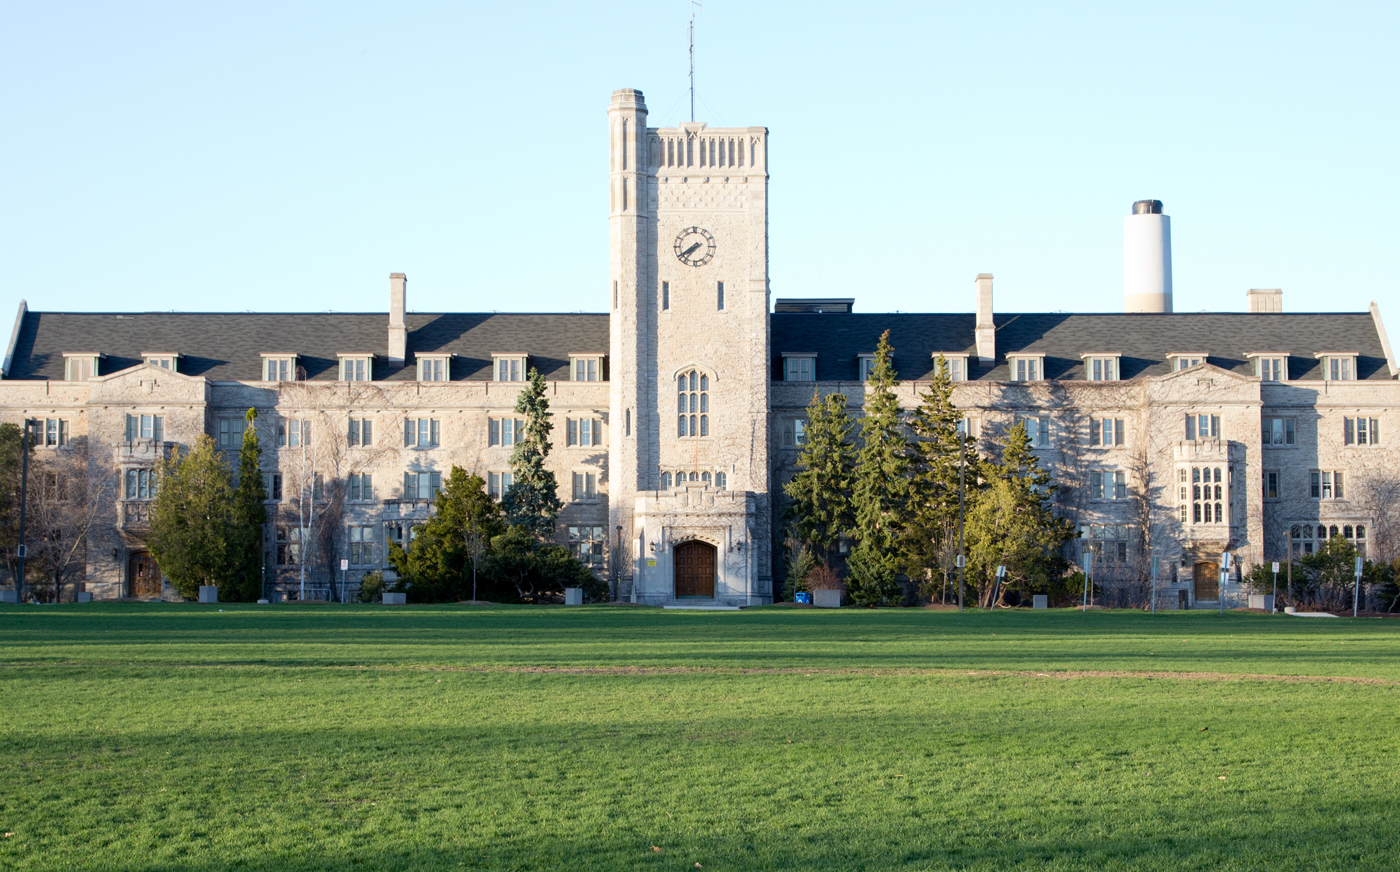
\includegraphics[height=\paperheight]{cover_jgreen.jpg}
%  }%
%}




%\makeindex
\begin{document}


%\BgThispage
% Some content
%\clearpage
%
%\pagebreak
%
\clearpage
%% temporary titles
% command to provide stretchy vertical space in proportion
\newcommand\nbvspace[1][3]{\vspace*{\stretch{#1}}}
% allow some slack to avoid under/overfull boxes
\newcommand\nbstretchyspace{\spaceskip0.5em plus 0.25em minus 0.25em}
% To improve spacing on titlepages
\newcommand{\nbtitlestretch}{\spaceskip0.6em}
\pagestyle{empty}
\begin{center}
\bfseries
\nbvspace[5]
\Huge
{\nbtitlestretch\huge
STATISTICS WITH APPLIED PROBABILITY\\
\hfill\\
Custom eBook for STA258}

%\nbvspace[1]
%\normalsize
\hfill\\[0.5em]

%EXTRA LINES\\
%EXTRA LINES EXTRA LINES EXTRA LINES\\
%EXTRA LINES EXTRA LINES
%\nbvspace[1]
%\small BY\\[1.5EM]
\nbvspace[1.5]
\LARGE
\textbf{Nishan Mudalige}\\[0.2em] 
\textbf{Nurlana Alili}\\[0.2em]
\textbf{Bryan Su}\\[0.5em]
\nbvspace[21]

%\nbvspace[2]




%\begin{tikzpicture}[line join=round, very thin]
%  \def\e{1260}
%  \foreach \x [evaluate={\i=mod(\x+90,360); \j=int((\i<180)*2-1); \t=3;
%    \sc=\x/\e; \n=int((\e-\x)/15+5); \X=\x/\e;}] in {10,25,...,\e} {
%
%    \path [shift={(3D cs:x=\x-\t,y={3*sin(\x-\t)})}, yslant=cos(\x)/5]
%      (-\X/2, 0)   coordinate (A')  ( \X/2, 0)   coordinate (B')
%      ( \X/2,2*\X) coordinate (C')  (-\X/2,2*\X) coordinate (D');
%
%    \path [shift={(3D cs:x=\x,y=3*sin \x)}, yslant=cos(\x)/5]
%      (-\X/2, 0)   coordinate (A) ( \X/2, 0)   coordinate (B)
%      ( \X/2,2*\X) coordinate (C) (-\X/2,2*\X) coordinate (D);
%
%    \filldraw [black!90] (B) -- (B') -- (C') -- (C)  -- cycle;
%    \filldraw [black!80] (A) -- (A') -- (D') -- (D)  -- cycle;
%    \filldraw [black!70] (C) -- (D)  -- (D') -- (C') -- cycle;
%    \filldraw [black]    (A) -- (B)  -- (C)  -- (D)  -- cycle;
%
%    \node [text=white, shift={($(C)!0.5!(D)$)}, anchor=north,
%      yslant=cos(\x)/5, font=\sf, scale=\sc*1.5] at (0,-.33*\X) {\n};
%  }
%  %
%  \foreach \i [evaluate={\x=\i*30-10; \X=1; \n=int(5-\i); \xsl=\x/180}]
%    in {1,...,4} {
%
%    \path [shift={(3D cs:x=\x+\e,y=-3*\x/90)}, yslant=cos \e/5, xslant=\xsl]
%      (-\X/2, 0)           coordinate (A) ( \X/2, 0)           coordinate (B)
%      ( \X/2, \X*2-\x/360) coordinate (C) (-\X/2, \X*2-\x/360) coordinate (D);
%
%    \path [shift={(3D cs:x=\x+\e,y=-3*\x/90)}, shift={(5/50,5/50-\i*2/50)},
%      yslant=cos \e/5, xslant=\xsl]
%      (-\X/2, 0)           coordinate (A') ( \X/2, 0)           coordinate (B')
%      ( \X/2, \X*2-\x/330) coordinate (C') (-\X/2, \X*2-\x/330) coordinate (D');
%
%    \filldraw [black!70] (C) -- (D)  -- (D') -- (C') -- cycle;
%    \filldraw [black!70] (A) -- (B)  -- (B') -- (A') -- cycle;
%    \filldraw [black!90] (B) -- (B') -- (C') -- (C)  -- cycle;
%    \filldraw [black]    (A) -- (B)  -- (C)  -- (D)  -- cycle;
%
%    \node [text=white, shift={($(C)!0.5!(D)$)}, anchor=north, xslant=\xsl,
%      yslant=cos \e/5, font=\sf, scale=1.5] at (0,-.33*\X) {\n};
%  }
%\end{tikzpicture}






%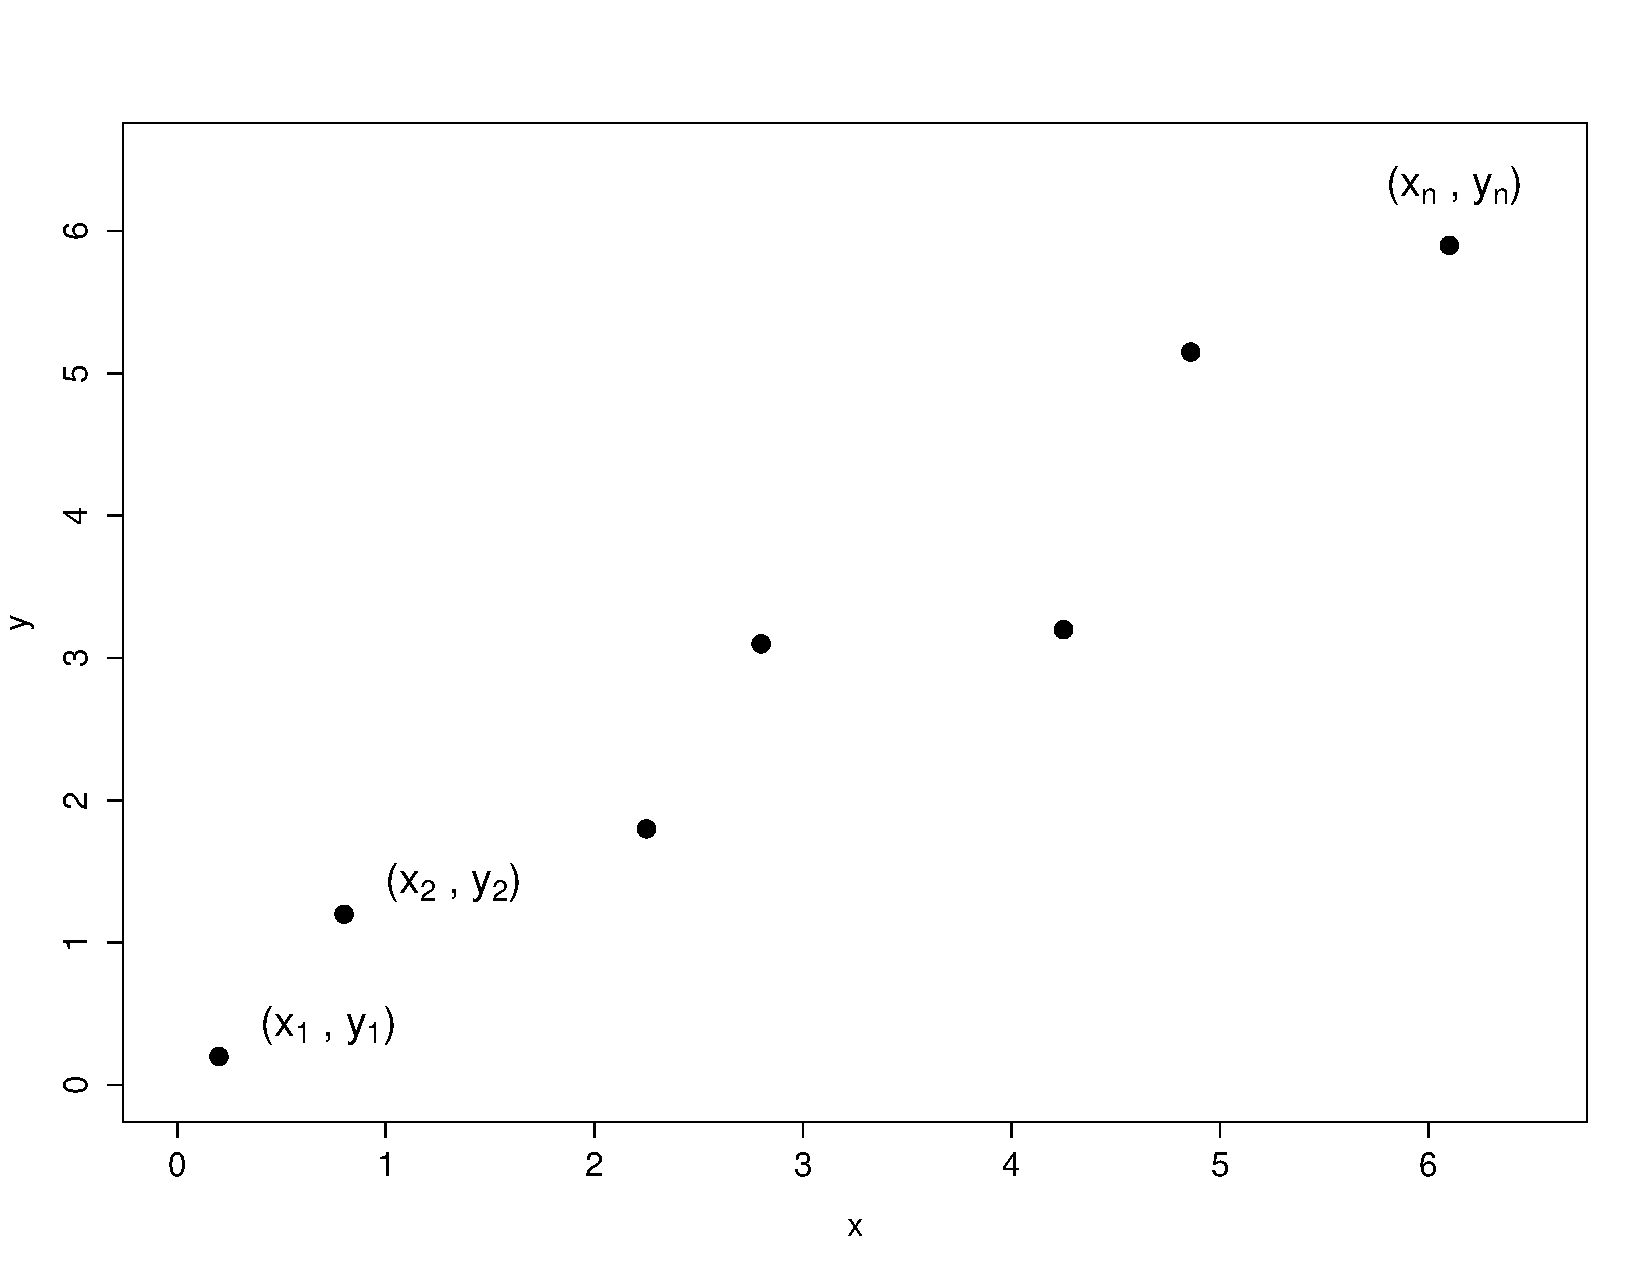
\includegraphics[width=1.5in]{Section8/XandYplotIncreasing.pdf}
%\nbvspace[3]
%\normalsize

%GUELPH, ON, CANA\\

\nbvspace[1]
%\hfill\\[0.5em]
\large
CANADA
\nbvspace[1]
\end{center}


%\clearpage
%\pagebreak
%\hfill
%\pagebreak





\title{\bf Statistics with Applied Probability\\
Custom eBook for STA258\\
\hfill\\}

\author{
Nishan Mudalige\\
{\it Department of Mathematical and Computational Sciences} \\
{\it University of Toronto Mississauga}\\[0.5em]
\ \\
Nurlana Alili\\
{\it University of Toronto Mississauga}\\[0.5em]
\ \\
Bryan Xu\\
{\it University of Toronto Mississauga}
}
\date{}


\maketitle


\newpage
\thispagestyle{empty}
%\tableofcontents

%\newpage
%\chapter*{Preface}

This book was based on OpenInto Statistics (Second Edition). A copy of OpenInto Statistics (Second Edition) may be downloaded as a free PDF at \href{http://www.openintro.org}{\color{black}\textbf{openintro.org}}.
\vspace{3mm}

\noindent We hope readers will take away three ideas from this book in addition to forming a foundation of statistical thinking and methods.\vspace{-1mm}
\begin{enumerate}
\setlength{\itemsep}{0mm}
\item[(1)] Statistics is an applied field with a wide range of practical applications.
%\item[(2)] You don't have to be a math guru to learn from real, interesting data.
\item[(2)] You don't have to be a math whiz to learn from real, interesting data.
\item[(3)] Data is messy, and statistical tools are imperfect. But, when you understand the strengths and weaknesses of these tools, you can use them to learn about the real~world.
\end{enumerate}


%\subsection*{Textbook overview}

%{\color{red}{
%The chapters of this book are as follows:
%\begin{description}
%\setlength{\itemsep}{0mm}
%\item[1. Introduction to data.] Data structures, variables, summaries, graphics, and basic data collection techniques.
%\item[2. Probability (special topic).] The basic principles of probability. An understanding of this chapter is not required for the main content in Chapters~\ref{modeling}-\ref{multipleAndLogisticRegression}.
%\item[3. Distributions of random variables.] Introduction to the normal model and other key distributions.
%\item[4. Foundations for inference.] General ideas for statistical inference in the context of estimating the population mean.
%\item[5. Inference for numerical data.] Inference for one or two sample means using the normal model and $t$ distribution, and also comparisons of many means using ANOVA.
%\item[6. Inference for categorical data.] Inference for proportions using the normal and chi-square distributions, as well as simulation and randomization techniques.
%\item[7. Introduction to linear regression.] An introduction to regression with two variables. Most of this chapter could be covered after Chapter~\ref{introductionToData}.
%\item[8. Multiple and logistic regression.] An introduction to multiple regression and logistic regression for an accelerated course.
%\end{description}
%} }


The chapters of this book are as follows:
\begin{description}
\setlength{\itemsep}{0mm}
\item[1. Overview.] General concept of inherent certainty and the power of prediction.
\item[1. Introduction to data.] Data structures, variables, types of studies and experimental design and basic data collection techniques.
%summaries, graphics, and basic data collection techniques.
\item[2. Descriptive statistics.] Numerical measures, graphical representations of data, data summaries
\item[3. Probability.] The basic principles of probability.
%An understanding of this chapter is not required for the main content in Chapters~\ref{modeling}-\ref{multipleAndLogisticRegression}.
\item[4. Distributions of random variables.] Commonly used distributions of discrete and continuous random variables. Introduction to the normal model and other key distributions.
\item[5. Basic Foundations for inference.] General ideas for statistical inference in the context of estimating the population mean. Emphasis on sampling theory.
\item[6. Confidence intervals.] One sample confidence intervals on the mean and on proportions; two sample confidence intervals on a difference of means on on a difference of proportions;
confidence intervals on paired data.
%\item[7. Inference for categorical data.] Inference for proportions using the normal and chi-square distributions, as well as simulation and randomization techniques.
%\item[8. Introduction to linear regression.] An introduction to regression with two variables. Most of this chapter could be covered after Chapter~\ref{introductionToData}.
%\item[9. Multiple and logistic regression.] An introduction to multiple regression and logistic regression for an accelerated course.
\end{description}

\emph{OpenIntro Statistics} was written to allow flexibility in choosing and ordering course topics. The material is divided into two pieces: main text and special topics. The main text has been structured to bring statistical inference and modeling closer to the front of a course. Special topics, labeled in the table of contents and in section titles, may be added to a course as they arise naturally in the curriculum.

\subsection*{Examples, exercises, and appendices}

Examples and within-chapter exercises throughout the textbook may be identified by their distinctive bullets:

\begin{example}{Large filled bullets signal the start of an example.}
Full solutions to examples are provided and often include an accompanying table or figure.
 \end{example}

\begin{exercise}
Large empty bullets signal to readers that an exercise has been inserted into the text for additional practice and guidance. Students may find it useful to fill in the bullet after understanding or successfully completing the exercise. Solutions are provided for all within-chapter exercises in footnotes.\footnote{Full solutions are located down here in the footnote!}
\end{exercise}

%There are exercises at the end of each chapter that are useful for practice or homework assignments. Many of these questions have multiple parts, and odd-numbered questions include solutions in Appendix~\ref{eoceSolutions}.

%There are exercises at the end of each chapter that are useful for practice or homework assignments. Many of these questions have multiple parts, and odd-numbered questions include solutions in Appendix~\ref{eoceSolutions}.

%There are exercises at the end of each chapter that are useful for practice or homework assignments. Many of these questions have multiple parts, and odd-numbered questions include solutions in Appendix~\ref{eoceSolutions}.


Probability tables for the normal, $t$, and chi-square distributions are in Appendix~\ref{distributionTables}, and PDF copies of these tables are also available from \href{http://www.openintro.org}{\color{black}\textbf{openintro.org}} for anyone to download, print, share, or modify.

\subsection*{OpenIntro, online resources, and getting involved}

OpenIntro is an organization focused on developing free and affordable education materials. \emph{OpenIntro Statistics}, our first project, is intended for introductory statistics courses at the high school through university levels.

We encourage anyone learning or teaching statistics to visit \href{http://www.openintro.org}{\color{black}\textbf{openintro.org}} and get involved. We also provide many free online resources, including free course software. Data sets for this textbook are available on the website and through a companion R package.\footnote{Diez DM, Barr CD, \c{C}etinkaya-Rundel M. 2012. \texttt{openintro}: OpenIntro data sets and supplement functions. \urlwofont{http://cran.r-project.org/web/packages/openintro}.} All of these resources are free, and we want to be clear that anyone is welcome to use these online tools and resources with or without this textbook as a companion.

We value your feedback. If there is a particular component of the project you especially like or think needs improvement, we want to hear from you. You may find our contact information on the title page of this book or on the \href{http://www.openintro.org/about.php}{About} section of \href{http://www.openintro.org}{\color{black}\textbf{openintro.org}}.

\subsection*{Acknowledgements}

This project would not be possible without the dedication and volunteer hours of all those involved. No one has received any monetary compensation from this project, and we hope you will join us in extending a \emph{thank you} to all those volunteers below.

The authors would like to thank Andrew Bray, Meenal Patel, Yongtao Guan, Filipp Brunshteyn, Rob Gould, and Chris Pope for their involvement and contributions. We are also very grateful to Dalene Stangl, Dave Harrington, Jan de Leeuw, Kevin Rader, and Philippe Rigollet for providing us with valuable feedback.



%\newpage

\newpage
\large





\begingroup
\small
\parindent 0pt
\parskip \baselineskip
\textcopyright{} 2025 N. Mudalige, N. Alili, B. Xu \\
All rights reserved.

This work may not be copied, translated, reproduced or transmitted
in any form or by any means --- graphic, electronic or mechanical including but not
limited to photocopying, scanning, recording, microfilming, electronic file sharing,
web distribution or information storage systems --- without the explicit 
written permission of the authors. 

Every effort has been made to trace ownership of all copyright material
and to secure permission from copyright holders.
In the event of any question arising as to the use of copyright material, we will be pleased
to make necessary corrections in future publications.

%    \lipsum[1-2]
%
%\begin{center}
% 99 32 11 88 48 01\hspace{2em}9 9 8 6 5 4 %1 
%\end{center}

\begin{center}
\begin{tabular}{ll}
First edition:  & August 2025 \\
%Second impression, with minor extensions & January 2009 \\
%Third impression, with minor extensions & May 2013 
\end{tabular}
\end{center}

%\vfill
\hfill

Mudalige, M.; Alili, N.; Xu, B.\\
%\hspace*{1em} Me, myself, and I / Jubobs. -- \\
\hspace*{1em} University of Guelph Bookstore Press\\
%\hspace*{2em} p. \hspace*{2em} cm. \\
%\hspace*{2em} Includes illustrations, bibliographical references and index. \\
%\hspace*{2em} ISBN \\
%\hspace*{2em} 1. Book design \hspace*{2em} I. Title


\vfill

University of Toronto Mississauga, \\
Mississauga, Ontario, Canada \\
%\texttt{publisher dot press (at) jubobs dot com}

%%%%{\LARGE\plogo}
\vspace*{2\baselineskip}


\endgroup
\clearpage





\setcounter{secnumdepth}{5}   
\setcounter{tocdepth}{5}
\tableofcontents


\pagebreak
\thispagestyle{empty}
\hfill\\
\pagebreak

%%%%%%%%%%%%%%
%% BOOK SECTIONS %%
%%%%%%%%%%%%%%



\large 
\setcounter{chapter}{-1}
\pagenumbering{arabic}\setcounter{page}{1}
\chapter{Overview}
\index{Overview}
%start relabeling as 2.1 etc
\pagestyle{myheadings}  

\setcounter{equation}{0}

\index{Statistics!Introduction}


Uncertainty is an inherent part of everyday life. 
We all face questions regarding uncertainty such as whether 
classes will go ahead as planned on any given day;
will a flight leave on time; 
will a student pass a certain course?
Uncertainties might also change depending on other factors, 
such as whether classes will still go ahead as planned when there is a snow warning in effect;
if a flight is delayed can a person still manage to make their connection;
will a student pass their course considering that the instructor is known to be a tough grader?\\

The ability to quantify uncertainty using rigorous mathematics is a powerful and useful tool.
Calculating uncertainty on an intuitive level is something that is hard-wired in our DNA, 
such as the decision to fight or flight depending on a given set of circumstances.
However we cannot always make such intuitive decisions
based purely on hunches and gut feelings.
Fortunes have been lost based on someone having a good feeling about something.
If we have information available, we should make the best prediction possible using this information.
For instance if we wanted to invest a lot of money in a company, we should use all available data such as
past sales, market and industry trends, leadership ability of the CEO, forward looking statements etc. 
and with all this information we can then predict whether our investment will be profitable.\\

In order for companies to survive and remain competitive in todays 
environment it is essential to monitor industry trends and read markets properly.
Companies that don't adapt and stick to an outdated business model
tend to pay the price.
At the other end of the spectrum, companies that understand the needs of the consumer, 
build their product around the consumer and keep evolving their product offerings based on
consumer trends tend to perform well and remain competitive.\\

Statistics is the science of uncertainty and it is clearly a very useful subject for business.
In this book you will be given an introduction to statistics and you will learn the
framework as well as the language required at the introductory level.
The material may be daunting at times, but the more you get familiar with the
subject the more comfortable you will become with it.
As business students, doing well in a statistics course will give you a competitive
edge since the ability to interpret and perform quantitative analytics are skills that are highly
desired by many employers.



\pagenumbering{arabic}
%\setcounter{page}{1}
\chapter{Descriptive Statistics and an Introduction to R}
\index{Introduction}
\label{sec.matrix}
%start relabeling as 2.1 etc
\pagestyle{myheadings}  \markboth{\ref{sec.matrix}.
\titleref{sec.matrix}}{}
%\setcounter{equation}{0}

\section{Introduction}

%\subsection{What is Statistics} \label{ssec.defm}\markright{\ref{ssec.defm} \titleref{ssec.defm}}

Intuitively, statistics can be considered the science of uncertainty. Formally,

\begin{definition}[Statistics]	\index{Statistics!Definition}
Statistics is the science of collecting, classifying, summarizing, analyzing and interpreting data.
\end{definition}

\noindent
\textbf{Population, Sample, Parameter}

\noindent
In statistics, researchers need to observe behavior, pattern, trends and other types of data to give a conclusion. To make the conclusion more persuasive, researchers require huge amount of data to support them, that's why study statistics need population. 

\begin{definition}[Population]
In statistics, a population is a set of similar observations which is of interest for some experimental questions. It can be a set of existing objects such as all people in Canada, or hypothetical group of existing objects such as the set of all possible hands in a game of poker. 
\end{definition}

\noindent
However, data collection from population is a lot work. Usually, researchers select a finite number of observations to study.

\begin{definition}[Sample]
It refers to a selection of a subset from population that researchers use it to estimate population characteristics.
\end{definition}

\noindent
Now, we have already chosen a sample, but how do we use it to estimate population characteristics? This is the point where parameter comes to play.

\begin{definition}[Parameter Statistics]
A parameter is a quantity of statistical population which summerizes characteristics of the population. For example, mean, variance and standard deviation.
\end{definition}

\noindent
\textbf{Descriptive and Inferential Statistics}

\noindent
Now, we have set everything we need. A population, a chosen sample in that population with its parameters. Next step is studying. There are two major types of analysis: descriptive and Inferential statistics. In this section, we are only going to give you a rough idea about what they are, more detailed materials will be introduced in later chapters.

\begin{definition}[Descriptive Statistics]
It refers to the summation of all quantitive values that describe characteristics of the population. Usually, we use descriptive statistics to summerize characteristics of a data set.
\end{definition}

\noindent
Furthermore, we use inferential statistics to do statistical analysis.

\begin{definition}[Inferential Statistics]
It refers to the process of using data analysis to indicate properties of a population. For example, testing hypothesis and confidence interval (both will be introduced in later chapters).
\end{definition}

\noindent
\textbf{Qualitative and Quantitative Data}

\noindent
At this point, assume that we have finished all procedures such as obtaining parameters and analyzing properties. Now, another important thing is illustrating all the discovery. 

\begin{definition}[Qualitative Data]
This type of illustration refers to showing categorical data. For example, lecture notes from a course, open-question survey. 
\end{definition}

\noindent
To illustrate numerical data, we use quantitative data.

\begin{definition}[Quantitative Data]
Unless the previous type of illustration, quantitative data is represented numerically, including anything that can be counted, measured, or given a numerical value. For example, STA258 final mark score range from 100 different students who have taken this course.
\end{definition}

\section{Descriptive Statistics}

\noindent
Previously, we defined descriptive statistics. Now, let's introduce what exact they are.\\

\noindent
\textbf{Sample Mean, Variance and Standard Deviation}

\noindent
Sample mean (or sample average) is the average value of a sample which is selected from an interested population of an experiment. Usually, the sample mean is used to estimate population mean. In other words, we say that the sample mean is an estimator of population mean.

\begin{definition}[Sample Mean]
 Let $x_1, x_2, x_3, ..., x_n$ be a sample of data points. We define sample mean of the sample data points ($\bar{x}$) as the following: \[ \bar{x} = \frac{1}{n} \sum_{i=1}^{n} x_i.\] Also, we define sample variance of the sample data points ($s^2$) as: \[ s^2 = \frac{1}{n-1} \sum_{i=1}^{n}(x_i - \bar{x})^2.\] Moreover, the standard deviation of the sample of data points ($s$) is: \[ s = \sqrt{s^2}, \quad \text{for } s > 0.\]
\end{definition}

\noindent
Now, let's move to variance. It refers to the expected value of the squared deviation from the mean of a random variable in a population. Similarly, we do have sample variance as well, which is the expected value of the squared deviation from the mean of a random variable in a selected sample. At this point, we can still use sample variance to estimate population variance with adjustment, because the sample variance may differ significantly based on what data points are chosen from that population.

\begin{definition}[Sample Variance]
Let $x_1, x_2, x_3, ..., x_n$ be a sample of data points, we define sample variance of the sample data points ($s^2$) as: \[ s^2 = \frac{1}{n-1} \sum_{i=1}^{n}(x_i - \bar{x})^2, \text{ where $\bar{x}$ is the sample mean of the data points.}\]
\end{definition}

\noindent
Next is standard deviation. It is a measure of the amount of variation of the values of a variable about its mean. If standard deviation is relatively larger, then data points are widely spread out from the mean. Otherwise, data points stay close from the mean. Also, standard deviation is obtained by taking squared root from variance which is dependent on the choices of data points as well. To use sample standard deviation as an estimator to population standard deviation, we still need to adjust it.

\begin{definition}[Sample Standard Deviation]
Let $x_1, x_2, x_3, ..., x_n$ be a sample of data points. The standard deviation of the sample of data points ($s$) is: \[ s = \sqrt{s^2}, \quad \text{for } s > 0.\]
\end{definition}

\noindent
\textbf{Median and Mode}

\noindent
The median and mode are two important measures of central tendency used in statistics to summarize and understand data. The median represents the middle value in a sorted dataset, giving a sense of the center that is not affected by extreme values or outliers. In contrast, the mode is the value that appears most frequently in a dataset, making it useful for identifying common or repeated observations.

\begin{definition}[Median]
Let: $x_1, x_2, x_3, ... , x_n$ be a collection of data points which is arranged in ascending order from the smallest value to the largest value (or descending order from the largest value to the smallest value in that collection). The median of the given collection of data points is the middle value in that collection, which equally spreads the collection into two parts. Half of all the collection values are above the median value and the rest of the values in the collection is below the median value.
\begin{itemize}
 \item Case 1: when n is an odd number. (i.e. $1, 3, 11, 237,...$). Then, the median $M$ is defined as: \[ M = \frac{n+1}{2} \text{, where n represents the $n^{th}$ position}.\]
 \item Case 2: when n is an even number (i.e. $2, 6, 100, 500,...$). Then, the median $M$ is: the average value of $\frac{n}{2}$'s and $\frac{n+2}{2}$'s position, where n represents the $n^{th}$ position.
 \end{itemize}
\end{definition}

\noindent
Now, let's introduce mode. 

\begin{definition}[Mode]
It refers to a value that appears the most frequent than the appearance of all other values in a given dataset.
\end{definition}

\noindent
\textbf{Percentile and Quartile}

\noindent
Percentiles and quartiles are statistical measures used to describe the distribution of data. A percentile indicates the value below which a given percentage of observations fall, helping to understand relative standing within a dataset. Quartiles, a specific type of percentile, divide the data into four equal parts (Q1, Q2/median, and Q3), providing insights into the spread and central tendency.

\begin{definition}[Percentile and Quartile]
Let: $x_1, x_2, ..., x_n$ be a collection of data points in either ascending order. Percentile is denoted as: $p^{th}$, which indicates $p \%$ of observations are below to a such value. Quartiles, are special cases of percentile which equally spread the collection of data into four parts. Each part contains $25\%$ of the entire collection. More specifically, we define quartiles as the following:
\begin{itemize}
 \item $Q_1$: the $25$ percentile (or $25^{th}$), which shows that $25\%$ of the data points are below the value $Q_1$.
 \item $Q_2$: the $50$ percentile (or $50^{th}$), which shows that $50\%$ of the data points are below the value $Q_2$.
 \item $Q_3$: the $75$ percentile (or $75^{th}$), which shows that $75\%$ of the data points are below the value $Q_3$.
 \item $Q_2$ is qual to median.
\end{itemize}
Moreover, we use $Q_3 - Q_1$ to calculate interquartile range (I.P.R), which shows the spread of the whole data set.
\end{definition}

\noindent
\textbf{Skewness and Symmetry}

\noindent
The two terms 'skewness' and 'symmetry' are used to describe the shape of probability distribution. There are two types of skewness: left (or negative) skew and right (or positive) skew. In real life, a famous distribution highly used in hypothesis testing which is $\chi_{n}^{2}$ with $n$ degrees of freedom, is right skewed probability distribution function. Another example regarding to symmetry is normal distribution such that its probability under its curve greater than $\mu$ is same as the probability below than $\mu$. Now let's introduce the proper definition of skewness and symmetry.

\begin{definition}[Skewness]
Skewness refers to such a measure of the asymmetry of the probability distribution of a real-valued random variable about its mean. The skewness value can be positive, zero, negative or undefined.
\end{definition}

\noindent
Now, let's break down the main definition of skewness and symmetry:

\begin{definition}[Left (or Negative) Skew]
By observing given probability distribution curve, if the left tail of the curve is longer than the right tail the mass of the distribution is concentrated on the right of the figure, then we say that probability distribution is left skew or negative skew. (See figure below)
\end{definition}

\begin{figure}[H]
\begin{center}
\begin{tikzpicture}
  \draw[thick, ->] (-1,0) -- (8,0) node[right] {$x$};
  \draw[thick, ->] (0,-0.2) -- (0,4) node[above] {$y$};

  \draw[thick, blue, smooth, samples=100, domain=0.5:7.5] 
    plot (\x, {3.5*exp(-0.6*(\x - 5)^2) + 0.6*exp(-0.3*(7 - \x))});
    
  \node at (3.8,-1.1) {\textbf{Left-Skewed Distribution}};
  
  \node at (2.4,1.2) {Long tail};
  \draw[->, thick] (2.8,0.9) -- (1.2,0.3);

  \node at (5.75,5) {Peak};
  \draw[->, thick] (5.5,4.5) -- (5.0,3.95);
\end{tikzpicture}
\end{center}
\caption{An illustration of a left (negative) skewed distribution.}
\end{figure}

\begin{definition}[Right (or Positive) Skew]
By observing given probability distribution curve, if the right tail of the curve is longer than the left tail the mass of the distribution is concentrated on the left of the figure, then we say that probability distribution is right skew or positive skew. (See figure below)
\end{definition}

\begin{figure}[H]
\begin{center}
\begin{tikzpicture}
  \draw[thick, ->] (-1,0) -- (8,0) node[right] {$x$};
  \draw[thick, ->] (0,-0.2) -- (0,4) node[above] {$y$};

  \draw[thick, blue, smooth, samples=100, domain=0.5:7.5] 
    plot (\x, {3.5*exp(-0.6*(\x - 3)^2) + 0.6*exp(-0.3*(\x - 2))});
    
  \node at (3.8,-0.5) {\textbf{Right-Skewed Distribution}};    

  \node at (2,4.5) {Peak};
  \draw[->, thick] (2.5,4.5) -- (3,4.1);

  \node at (6.7,0.9) {Long tail};
  \draw[->, thick] (6.5,0.6) -- (7.2,0.4);
\end{tikzpicture}
\end{center}
\caption{An illustration of a right (positive) skewed distribution}
\end{figure}

\noindent
Symmetry is a special case of skewness when the value of skewness is $0$.

\begin{definition}[Symmetry]
In statistics, symmetry s a probability distribution is reflected around a vertical line at some value of the random variable represented by the distribution. Probability under the curve below that value is equal to probability under the curve greater than that value. (see figure below)
\end{definition}

\begin{figure}[h]
\begin{center}
\begin{tikzpicture}[xscale=1.5, yscale=6]
  \draw[->, thick] (-3.2,0) -- (3.2,0) node[right] {$x$};
  \draw[->, thick] (0,0) -- (0,0.45) node[above] {$f(x) = \text{peak}$};

  \draw[domain=-3:3, smooth, variable=\x, blue, thick] 
    plot ({\x}, {1/sqrt(2*pi) * exp(-0.5*\x*\x)});

  \draw[dashed] (0,0) -- (0,{1/sqrt(2*pi)});
  \node[below] at (0,0) {$\mu = 0$};
\end{tikzpicture}
\end{center}
\caption{An illustration of symmetric distribution. Area under this curve on the left hand side of $\mu = 0$ is same as the area on the right hand side under the curve.}
\end{figure}

\noindent
Since symmetry is a special case, so that it has a unique property as the following:

\begin{thm}[Empirical Rule (or $68-95-99.7$ Rule)]
For any symmetric (bell-shaped) curve, let $\mu$ be its mean and $\sigma$ be its standard deviation, the following probability set function is true:
   \begin{itemize}
    \item  $1.$ $P(\mu - \sigma < X < \mu + \sigma) = 68.27\%;$
    \item  $2.$ $P(\mu - 2\sigma < X < \mu + 2\sigma) = 95.45\%;$
    \item  $3.$ $P(\mu - 3\sigma < X < \mu + 3\sigma) = 99.73\%.$
   \end{itemize}
\end{thm}

\begin{figure}[h]
\begin{center}
\begin{tikzpicture}[xscale=1.8, yscale=6]
  \draw[->, thick] (-3.5,0) -- (3.5,0) node[right] {$x$};
  \draw[->, thick] (0,0) -- (0,0.45) node[above] {$f(x) = \text{peak}$};

  \draw[domain=-3.2:3.2, smooth, variable=\x, thick, blue] 
    plot ({\x}, {1/sqrt(2*pi) * exp(-0.5*\x*\x)});

  \fill[green!40, opacity=0.7] 
    plot[domain=-1:1] (\x, {1/sqrt(2*pi) * exp(-0.5*\x*\x)}) -- (1,0) -- (-1,0) -- cycle;

  \fill[orange!40, opacity=0.7] 
    plot[domain=-2:-1] (\x, {1/sqrt(2*pi) * exp(-0.5*\x*\x)}) -- (-1,0) -- (-2,0) -- cycle;
  \fill[orange!40, opacity=0.7] 
    plot[domain=1:2] (\x, {1/sqrt(2*pi) * exp(-0.5*\x*\x)}) -- (2,0) -- (1,0) -- cycle;

  \fill[cyan!40, opacity=0.7] 
    plot[domain=-3:-2] (\x, {1/sqrt(2*pi) * exp(-0.5*\x*\x)}) -- (-2,0) -- (-3,0) -- cycle;
  \fill[cyan!40, opacity=0.7] 
    plot[domain=2:3] (\x, {1/sqrt(2*pi) * exp(-0.5*\x*\x)}) -- (3,0) -- (2,0) -- cycle;

  \foreach \x in {-3,-2,-1,0,1,2,3} {
    \draw[dashed] (\x,0) -- (\x,{1/sqrt(2*pi) * exp(-0.5*\x*\x)});
    \node[below] at (\x,0) {\x$\sigma$};
  }

  \node at (0,0.32) {\textbf{68\%}};
  \node at (-1.5,0.22) {13.5\%};
  \node at (1.5,0.22) {13.5\%};
  \node at (-2.5,0.22) {2.35\%};
  \node at (2.5,0.22) {2.35\%};
  \node at (-3.25,0.22) {0.15\%};
  \node at (3.25,0.22) {0.15\%};

  \node[font=\bfseries] at (0,-0.1) {Empirical Rule (68–95–99.7)};
\end{tikzpicture}
\end{center}
\caption{An illustration of the empirical rule.}
\end{figure}

\textbf{Practice Example}

\begin{example}[Calculating Sample Mean, Variance and Standard Deviation]
Let: $x_1 = 1, x_2 = 3$ and $x_3 = 7$. Calculate the sample mean, sample variance and sample standard deviation for this collection of data points.\\
Solution (all results are kept in four digits):\\
By Definition $1.9 \text{, } 1.10 \text{, } 1.11$, sample mean: \[ \bar{x} = \frac{1+3+7}{3} \approx 3.6667.\]
Then, we use sample mean to calculate sample variance: \[ s^2 = \frac{1}{3-1} \times [(1-3.6667)^2+(3-3.6667)^2+(7-3.6667)^2] \approx 9.3333.\]
Finally, we take the square root of sample variance to get sample deviation, and remember that $s > 0$: \[ s = \sqrt{s^2} \approx 3.0551.\]
\end{example}

\begin{example}[Median Calculation]
Given two distinct collections of data points: $S_1$ = $\{2, 4, 6\}$ and $S_2$ = $\{1, 5, 16, 28\}$. Calculate the median of both two sets.\\
Solution: \\
For $S_1$, since $n = 3$ which is an odd number, so by $Definition \text{ } 1.3$, $M_{S_1} = 4$. For $S_2$, $n = 4$ in this case, so that we need to calculate the average of $\frac{n}{2}$ and $\frac{n+1}{2}$. Then, \[ M_{S_2} = \frac{5+16}{2} = 10.5.\]
\end{example}

\begin{example}
Consider the data set $S = $ $\{4, 25, 30, 30, 30, 32, 32, 35, 50, 50, 50, 55, 60, 74, 110\}$. Calculate its median and $Q_1$ ($25^{th}$).\\
Solution:\\
Simply counting the number of data points, $n = 15$, such that $M_{S}$ = $\frac{15 + 1}{2}$ = $8$. Thus, the $8^{th}$ value in the set which is $35$.\\
Since we know the median of this collection of data points, we just need to find the median of the lower half of this data, which is exactly going to be $25$ percentile ($25^{th}$). In the lower half of the given collection (all values below the median), $n_{lower} = 7$. By $Definition \text{ } 1.3$, then median of the lower half ($25^{th}$) is going to be: \[ 25^{th} = \frac{7+1}{2} = 4, \text{ the $4^{th}$ position in the data set}.\] Thus, $Q_1$ ($25^{th}$) $= 30$. To find $Q_3$ ($75^{th}$), apply the same strategy will guide you to find the correct answer, and we leave this as an exercise to you.
\end{example}

\section{Graphical Techniques}

In statistics, there are lots of types of graph to illustrate data, for example histograms and box-plots. This technique is used in the field of statistics for data visualization. Our objective is to both be able to identify some classical types of graph and interpret key statistical values (descriptive statistical values) from it.

\subsection{Histograms}

\textbf{Introduction to Histograms}

\noindent
Histogram is a graphical representation of data that uses bars to display the frequency distribution of a dataset. Unlike bar graphs, which represent categorical data, histograms group numerical data into intervals (bins) and show how many values fall into each range. This makes histograms ideal for visualizing the shape, spread, and central tendency of continuous data, helping identify patterns such as symmetry, skewness, and outliers.\\

\begin{figure}[h]
\begin{center}
\begin{tikzpicture}
  \draw[->] (0,0) -- (7.5,0) node[right] {Value};
  \draw[->] (0,0) -- (0,5.5) node[above] {Frequency};

  \filldraw[fill=blue!30] (0.5,0) rectangle (1.5,2);
  \filldraw[fill=blue!30] (1.5,0) rectangle (2.5,3.5);
  \filldraw[fill=blue!30] (2.5,0) rectangle (3.5,5);
  \filldraw[fill=blue!30] (3.5,0) rectangle (4.5,4);
  \filldraw[fill=blue!30] (4.5,0) rectangle (5.5,2.5);
  \filldraw[fill=blue!30] (5.5,0) rectangle (6.5,1);

  \foreach \x/\label in {1/10, 2/20, 3/30, 4/40, 5/50, 6/60} {
    \draw (\x,0) -- (\x,-0.2);
    \node[below] at (\x, -0.2) {\label};
  }

  \foreach \y in {1,...,5} {
    \draw (0,\y) -- (-0.15,\y);
    \node[left] at (-0.2,\y) {\y};
  }
\end{tikzpicture}
\end{center}
\caption{An illustration of histogram.}
\end{figure}

\textbf{Advantages and Disadvantages of Histograms}

\begin{itemize}
 \item Advantages of Histograms:\\
 $1.$ Histograms are easily to used for visualise data (relatively). It allows us to get the idea of the "shape" of distribution (i.e. skewness which will be discussed late in this section).\\
 $2.$ It is also flexible that people are able to modify bin widths.
 \item Disadvantages of Histograms:\\
 $1.$ It is not suitable for small data sets.\\
 $2.$ The values from histograms close to breaking points are likely similar, in fact they need to be classified into different bins (i.e. Student A and B scores 79 and 80 respectively in   STA258, we consider a breaking point between 79 and 80. The two students have similar score, but student A is $B+$ and student B is $A-$ in GPA from).
 \end{itemize}
 
\textbf{Histograms with Skewness and Symmetry}

A histogram visually represents the distribution of numerical data, making it a useful tool for assessing skewness and symmetry. It is quite straightforward to estimate the skewness of histograms by simply drawing a curve above bins on the histogram.


Case 1: A histogram has a left (negative) skewed probability distribution:
\begin{figure}[H]
\begin{center}
\begin{tikzpicture}[xscale=1.2, yscale=1]
  \draw[->] (0,0) -- (7.5,0) node[right] {Value};
  \draw[->] (0,0) -- (0,5.5) node[above] {Frequency};
  \filldraw[fill=blue!30] (0.5,0) rectangle (1.5,1);
  \filldraw[fill=blue!30] (1.5,0) rectangle (2.5,2);
  \filldraw[fill=blue!30] (2.5,0) rectangle (3.5,3);
  \filldraw[fill=blue!30] (3.5,0) rectangle (4.5,4.2);
  \filldraw[fill=blue!30] (4.5,0) rectangle (5.5,4.7);
  \filldraw[fill=blue!30] (5.5,0) rectangle (6.5,4.9);
  \foreach \x/\label in {1/10, 2/20, 3/30, 4/40, 5/50, 6/60} {
    \draw (\x,0) -- (\x,-0.15);
    \node[below] at (\x,-0.3) {\label};
  }
  \foreach \y in {1,...,5} {
    \draw (0,\y) -- (-0.1,\y);
    \node[left] at (-0.3,\y) {\y};
  }
  \draw[thick, red, smooth, samples=100, domain=0.7:6.3] 
    plot (\x, {5*exp(-0.3*(6.5 - \x)^2) + 0.5*exp(-0.3*(\x - 1.5))});
  \node[font=\bfseries] at (3.75,-1.8) {Left-Skewed Histogram with Overlay Curve};
\end{tikzpicture}
\end{center}
\caption{An illustration of a histogram to have a left (or negative) skew probability distribution.}
\end{figure}

Case 2: A histogram has a right (positive) skewed probability distribution:
\begin{figure}[h!]
\begin{center}
\begin{tikzpicture}[xscale=1.2, yscale=1]
  \draw[->] (0,0) -- (7.5,0) node[right] {Value};
  \draw[->] (0,0) -- (0,5.5) node[above] {Frequency};

  \filldraw[fill=blue!30] (0.5,0) rectangle (1.5,4.9);
  \filldraw[fill=blue!30] (1.5,0) rectangle (2.5,4.5);
  \filldraw[fill=blue!30] (2.5,0) rectangle (3.5,3.8);
  \filldraw[fill=blue!30] (3.5,0) rectangle (4.5,2.8);
  \filldraw[fill=blue!30] (4.5,0) rectangle (5.5,1.8);
  \filldraw[fill=blue!30] (5.5,0) rectangle (6.5,1);

  \foreach \x/\label in {1/10, 2/20, 3/30, 4/40, 5/50, 6/60} {
    \draw (\x,0) -- (\x,-0.15);
    \node[below] at (\x,-0.3) {\label};
  }

  \foreach \y in {1,...,5} {
    \draw (0,\y) -- (-0.1,\y);
    \node[left] at (-0.3,\y) {\y};
  }

  \draw[thick, red, smooth, samples=100, domain=0.7:6.3] 
    plot (\x, {5*exp(-0.3*(\x - 1.5)^2) + 0.5*exp(-0.3*(6.5 - \x))});
  \node[font=\bfseries] at (3.75,-1.8) {Right-Skewed Histogram with Overlay Curve};
\end{tikzpicture}
\end{center}
\caption{An illustration of a histogram to have a right (or positive) skew probability distribution.}
\end{figure}

Case 3: A histogram has a symmetric skewed probability distribution:

\begin{figure}[h]
\begin{center}
\begin{tikzpicture}[xscale=1.2, yscale=1]
  \draw[->] (0,0) -- (7.5,0) node[right] {Value};
  \draw[->] (0,0) -- (0,5.5) node[above] {Frequency};
  \filldraw[fill=blue!30] (0.5,0) rectangle (1.5,2.5);
  \filldraw[fill=blue!30] (1.5,0) rectangle (2.5,4);
  \filldraw[fill=blue!30] (2.5,0) rectangle (3.5,5);
  \filldraw[fill=blue!30] (3.5,0) rectangle (4.5,4);
  \filldraw[fill=blue!30] (4.5,0) rectangle (5.5,2.5);
  \foreach \x/\label in {1/10, 2/20, 3/30, 4/40, 5/50} {
    \draw (\x,0) -- (\x,-0.15);
    \node[below] at (\x,-0.3) {\label};
  }
  \foreach \y in {1,...,5} {
    \draw (0,\y) -- (-0.1,\y);
    \node[left] at (-0.3,\y) {\y};
  }
  \draw[thick, red, smooth, samples=100, domain=0.7:5.3]
    plot (\x, {5*exp(-0.5*(\x - 3)^2)});
  \node[font=\bfseries] at (3.75,-1.8) {Symmetric Histogram with Overlay Curve};
\end{tikzpicture}
\end{center}
\caption{An illustration of a histogram which has a symmetric probability distribution.}
\end{figure}

\subsection{Box-Plots}
A boxplot (or box-and-whisker plot) is a standardized way to display data distribution based on a five-number summary: minimum, first quartile (Q1), median (Q2), third quartile (Q3), and maximum. The box represents the interquartile range (IQR), while the whiskers show variability outside Q1 and Q3. Outliers are plotted as individual points. Boxplots efficiently compare distributions and highlight skewness, spread, and outliers. (See figure below)

\begin{figure}[H]
 \centering
 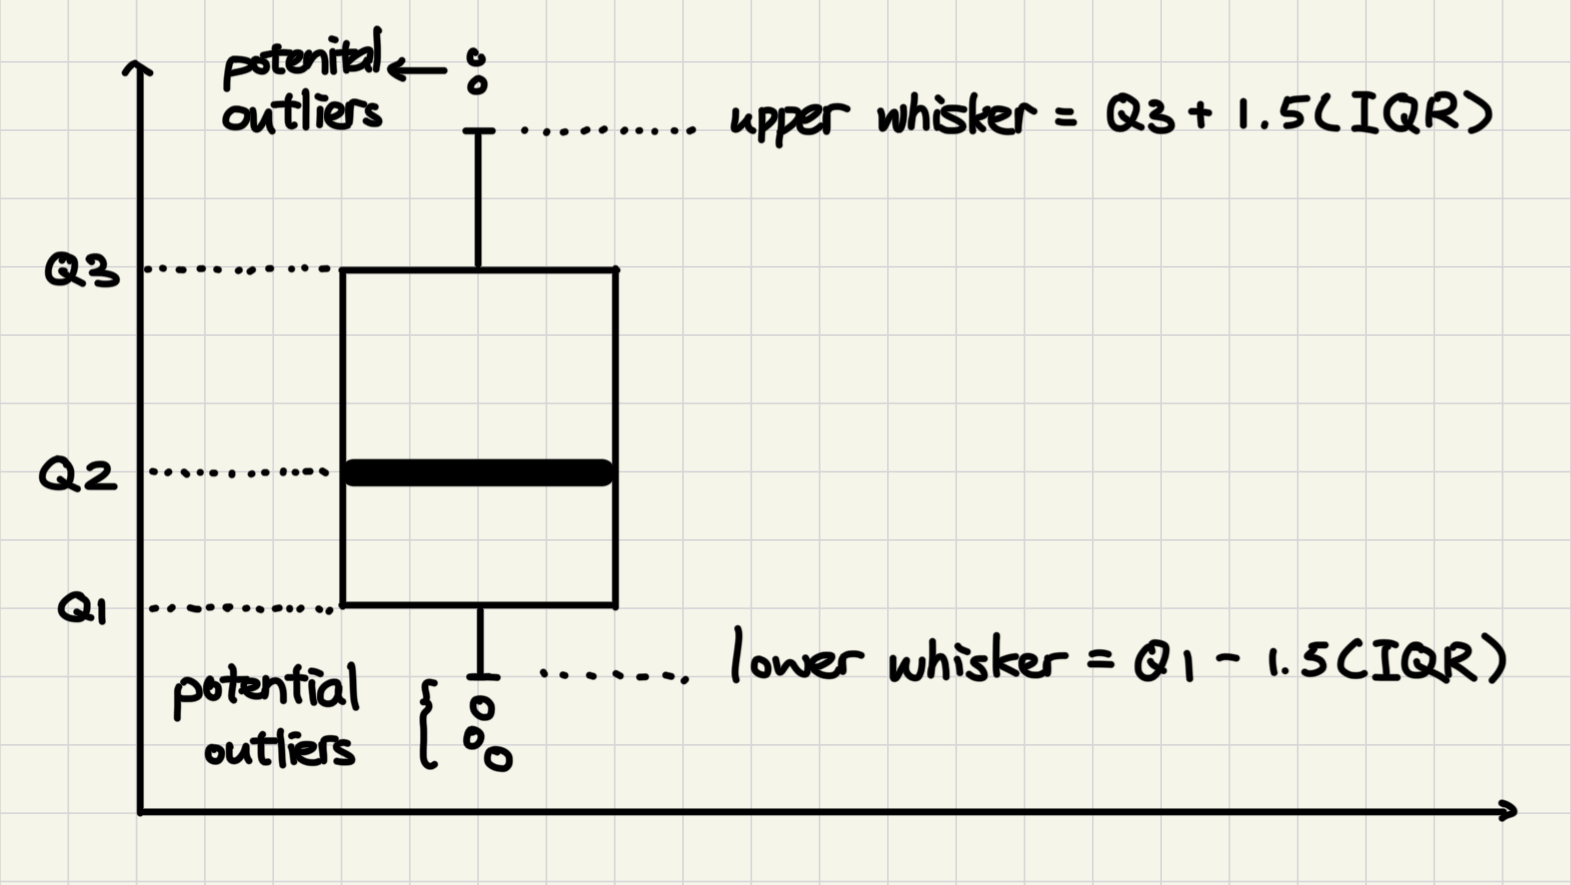
\includegraphics[scale=0.25]{Section1/img/BoxPlot.jpg}
 \caption{Visualization of a box-plot}
\end{figure} 

\noindent
Similar to histograms, we can still obtain information about skewness and symmetry, by observing the cut from the line of Q2.\\

\noindent
If the median (Q2) cuts the box with upper area smaller than lower area, then we say that box-plot with left skew probability distribution. Or, if the median (Q2) cuts the box with upper area larger than lower area, then we say that box-plot with right skew probability distribution.\\

\noindent
Otherwise, if the median (Q2) cuts the box with upper area equal to lower area, then we say that box-plot with symmetric probability distribution.

\begin{figure}[H]
\centering
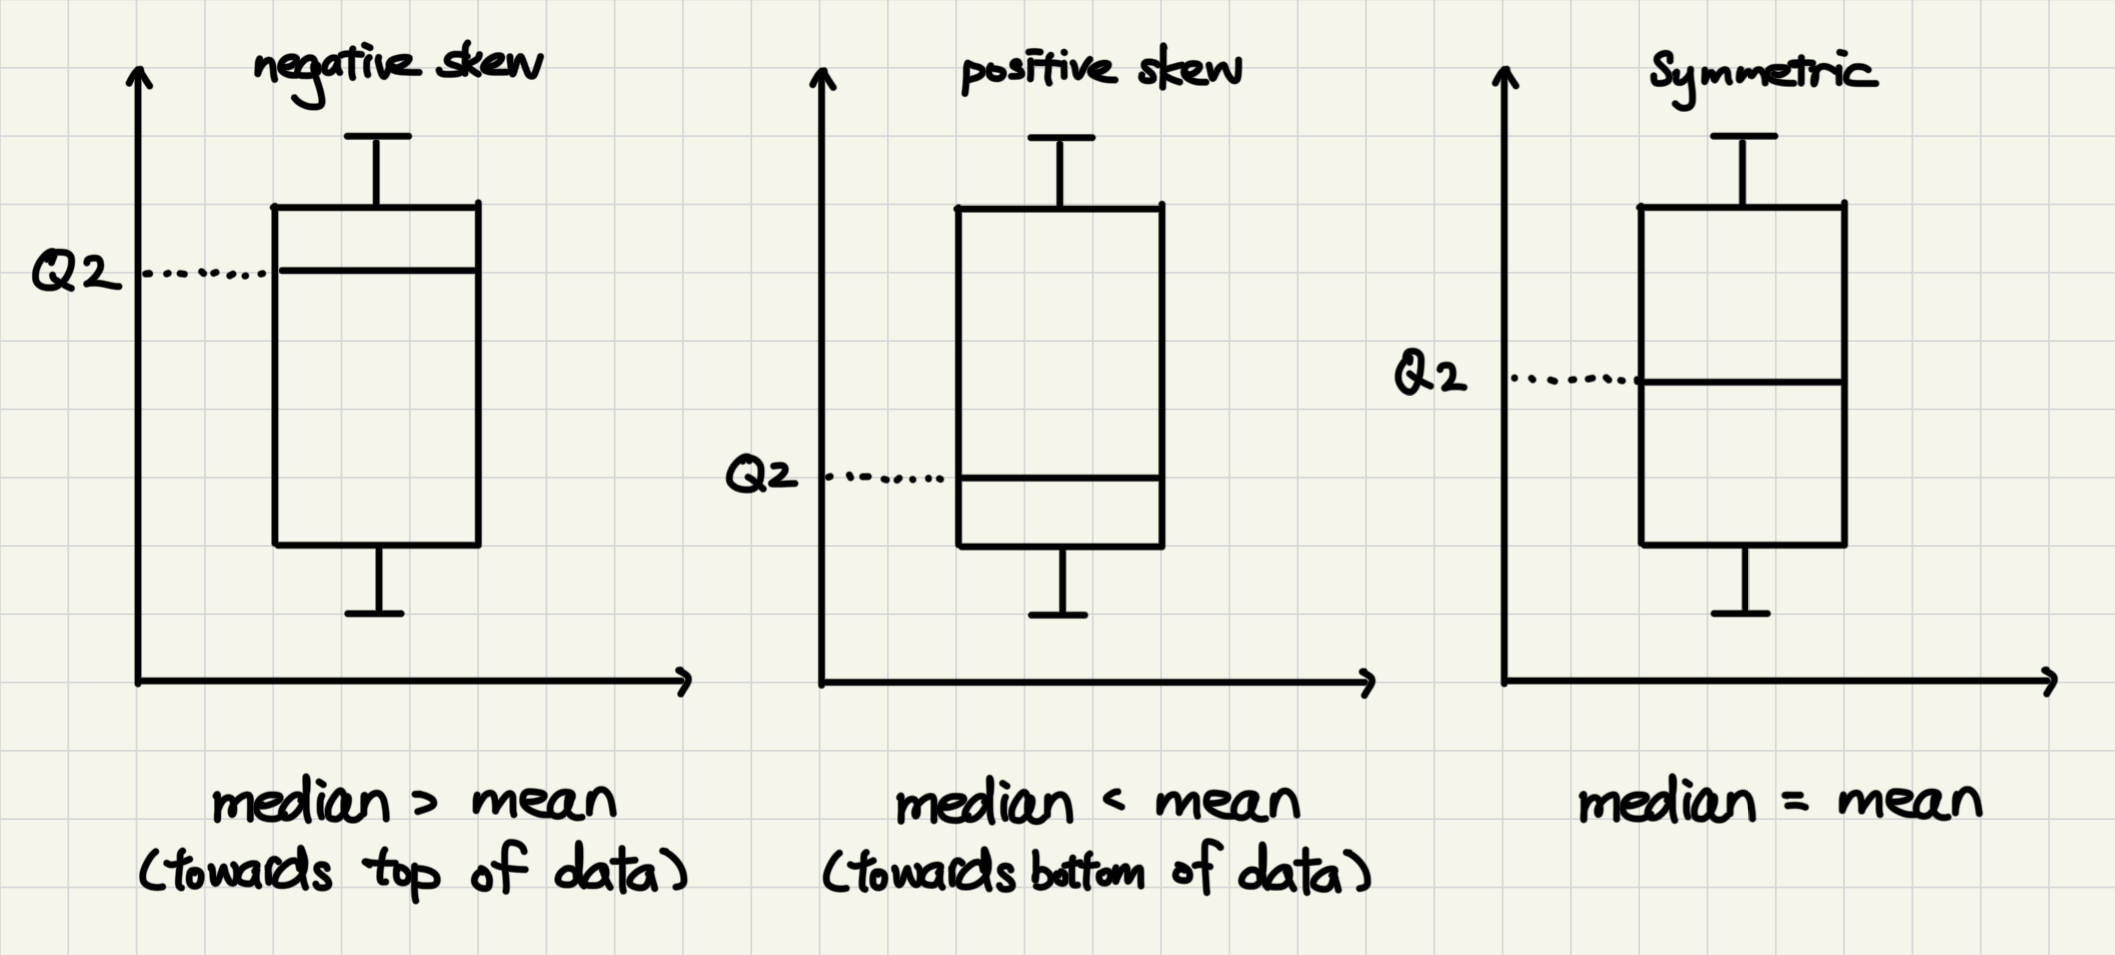
\includegraphics[scale=0.15]{Section1/img/Bskew.jpg}
\caption{Visualization of a box-plot with skew and symmetric probability distribution}
\end{figure}

\section{Introduction to R}

R is used for data manipulation, statistics, and graphics. It is made of: operations ($+$,$ -$, $<$) which is for calculations on vectors, arrays and matrices; a huge collection of functions; facilities for making unlimited types quality graphs; user contributed packages (sets of related functions); the ability to interface with procedures written in C, C+, or FORTRAN and to write additional primitives. R is also an open-source computing package which has seen a huge growth in popularity in the last few years (Please use this website: https://cran.r-project.org, to download R).\\

\noindent
\textbf{What is R-studio?}

\noindent
RStudio is a relatively new editor specially targeted at R. RStudio is cross-platform, free and open-source software (Please use: https://www.rstudio.com, to download Rstudio).\\

\noindent
\textbf{Make a Histogram Using R-studio}

\noindent
This is just a demonstration of how to start and use R-studio. 

\noindent
1. First of all, we need to know which dataset are we going to make into a histogram. In this case, as an example, we are going to use the waiting time in faithful in R-studio.\\
2. For any dataset, use the code: names(faithful) to get it. (inside the parentheses, type the names of variables you want in faithful dataset)\\
3. Then, we proceed with the code: hist(faithful\$waiting) to get a basic plot.\\

\begin{figure}[H]
 \centering
 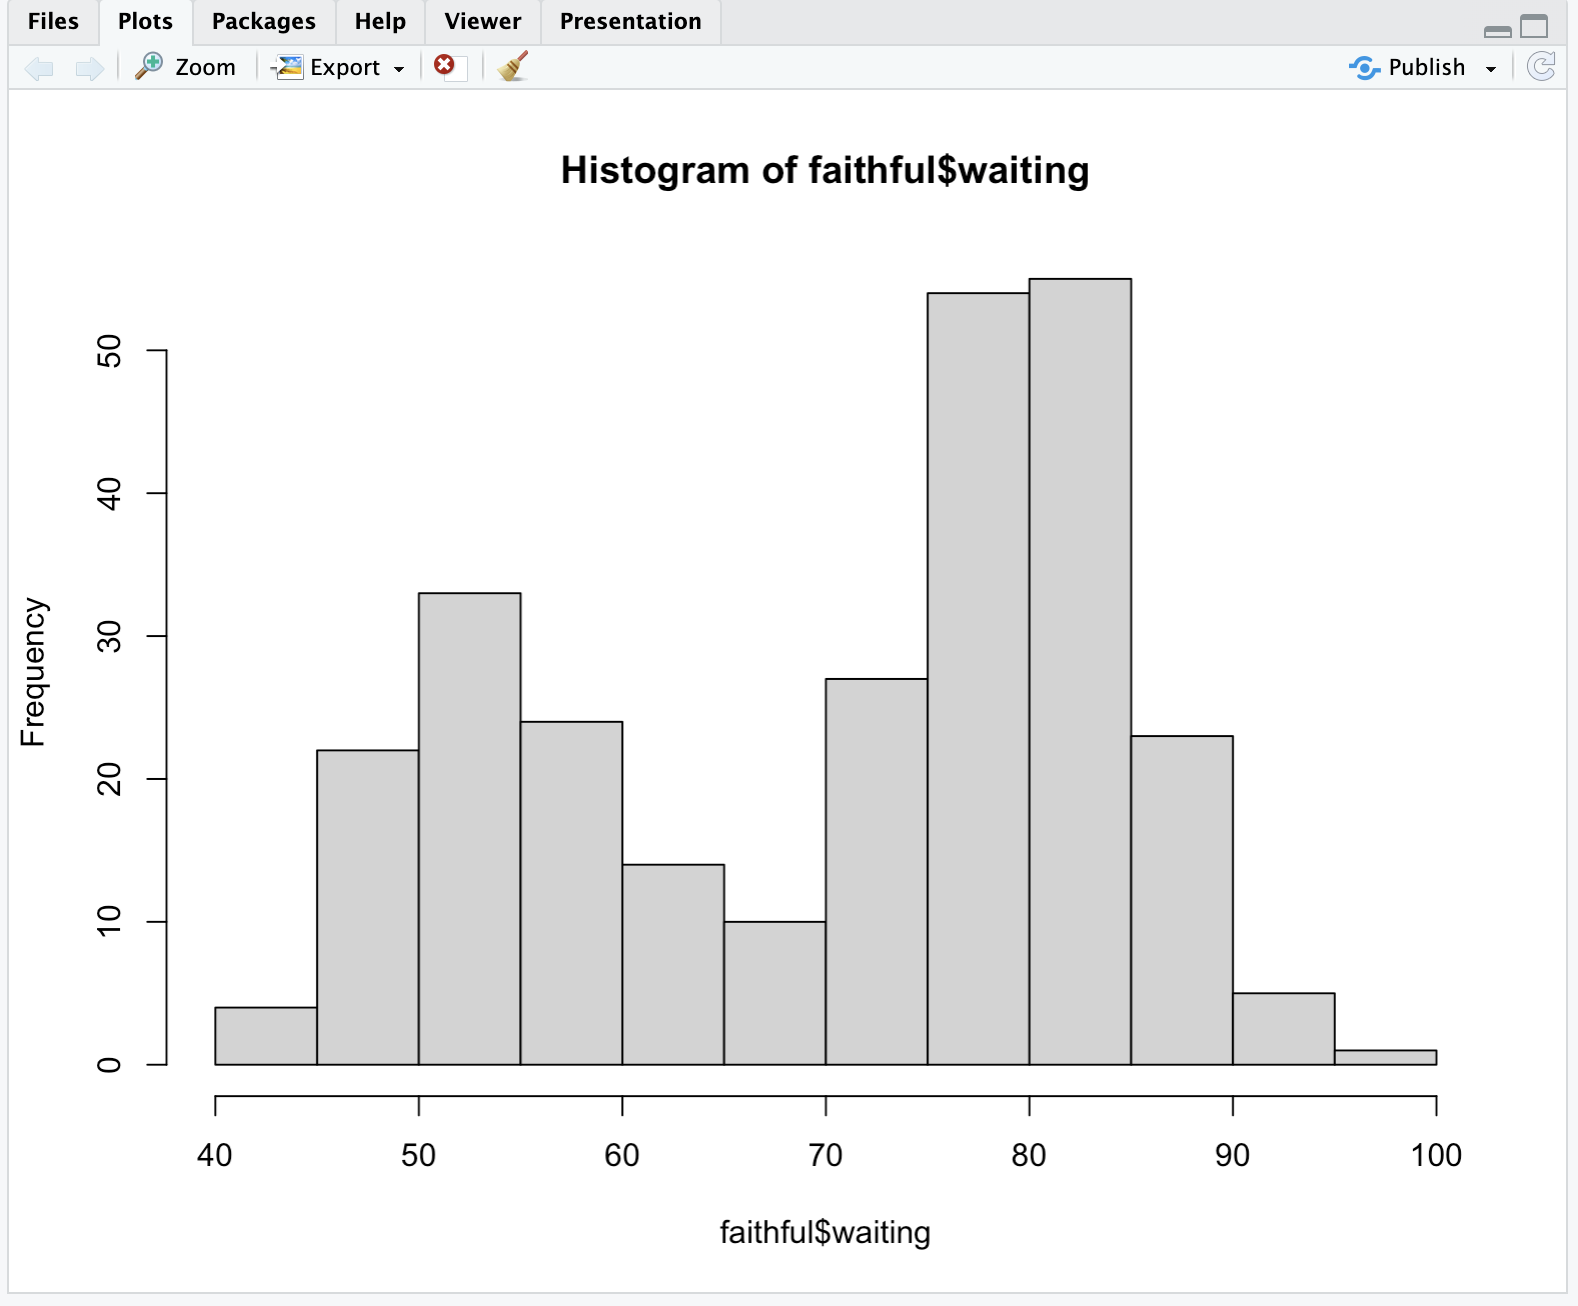
\includegraphics[scale=0.45]{Section1/img/R1.jpg}
 \caption{R-studio first three steps (by following the instructions, you should get this histogram)}
\end{figure}

\noindent
4. Furthermore, we can also get more information. For example, by keep proceeding with the code: hist(faithful\$waiting,plot=FALSE)\$breaks, R-studio will show you all the breaking points between histogram cells.

\begin{figure}[H]
 \centering
 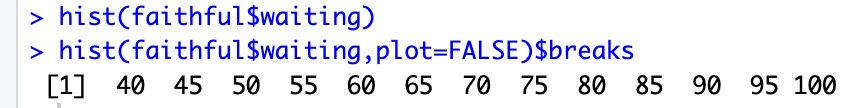
\includegraphics[scale=0.45]{Section1/img/R2.jpg}
 \caption{R-studio the forth step(by following the instructions, you should get this histogram)}
 \end{figure}

%%\pagenumbering{arabic}
%\setcounter{page}{1}
\chapter{Sampling Distributions Related to a Normal Population}
%\index{Introduction}
%\label{sec.matrix}
%start relabeling as 2.1 etc
%\pagestyle{myheadings}  \markboth{\ref{sec.matrix}.
%\titleref{sec.matrix}}{}
%\setcounter{equation}{0}

Previously, we have introduced lots of definitions and given you a rough idea about what really statistics it and what people do in statistics. Now, we are going to proceed statistical distributions. 

\section{Normal Distribution}

In probability theory and statistics, normal distribution also called Gaussian distribution which is discovered by a famous German mathematician Johann Carl Friedrich Gauss in 1809. It is one of the most important distribution that used to approximate other types of probability distribution, such as binomial, hypergeometric, inverse (or negative) hypergeometric, negative binomial and Poisson distribution. Generally, it is denote as $N(\mu, \sigma^2)$ with probability density function as the following: \[ f(x) = \frac{1}{\sqrt{2 \pi \sigma^2}} \cdot e^{-\frac{(x - \mu)^2}{2\sigma^2}}.\]
Formally, let's begin with its definition:

\begin{definition}[Normal Distribution]
Suppose a random variable $X \sim N(\mu, \sigma^2)$, then $E(X) = \mu \text{ and } Var(X) = \sigma^2$. And $-\infty < \mu < \infty, \sigma^2 > 0.$ Moreover, $X$ has probability density function as: \[ f(x) = \frac{1}{\sqrt{2 \pi \sigma^2}} \cdot e^{-\frac{(x - \mu)^2}{2\sigma^2}}, \text{ for $-\infty < x < \infty$ (same as above).}\]
The only special case of normal distribution is standard normal distribution, such that a random variable $Y \sim N( \mu = E(Y) = 0, \sigma^2 = Var(Y) = 1)$, then $Y$ has probability density function as: \[ f(y) = \frac{1}{\sqrt{2\pi}} \cdot e^{-\frac{y^2}{2}}.\]
\end{definition}

\section{Gamma and Chi-square Distribution}

The Chi-square and Gamma distributions are two fundamental probability distributions widely used in statistical theory and applications. The Gamma distribution is a continuous distribution characterized by its shape and scale parameters, making it versatile for modeling waiting times and various positively skewed data. The Chi-square distribution, a special case of the Gamma distribution, arises naturally in the context of hypothesis testing and confidence interval estimation, especially in tests involving variance and categorical data.\\

\noindent
\textbf{Gamma Distribution}

\begin{definition}[Gamma Distribution]
Suppose a random variable $X$ is Gamma distributed with $\alpha > 0$ (shape parameter) and $\beta > 0$ (scale parameter) if and only if the probability density function of $X$ is \[ f(x) = \frac{x^{\alpha - 1} e^{\frac{-x}{\beta}}}{\beta^{\alpha} \Gamma(\alpha)}, \text{ for $0 < x < \infty.$}\]
Then, $E(X) = \alpha \beta \text{, } Var(X) = \alpha \beta^2 \text{ and its moment generating function is } M_{X}(t) = \frac{1}{(1 - \beta t)^{\alpha}},$ for $t < \frac{1}{\beta}.$
\end{definition}

\noindent
Now, let's introduce some properties of Gamma function:

\begin{itemize}
	\item Gamma function (\textbf{not a distribution}): \[ \Gamma(x) = \int_{0}^{\infty}t^{x-1}e^{-t}\,dt, \text{ for $x > 0$.} \]
	\item Properties
		\begin{itemize}
			\item 1. $\Gamma(x) = x \cdot \Gamma(x-1)$;
			\item 2. For all $n \in \mathbb{N} \text{, } \Gamma(n) = (n - 1)!$; 
			\item 3. $\Gamma(\frac{1}{2}) = \sqrt{\pi}$.
		\end{itemize}
\end{itemize}

\noindent
\textbf{Chi-square Distribution}

\noindent
Here is its formal definition:

\begin{definition}[Chi-square Distribution]
A random variable $X$ has a Chi-squared distribution with $n$ degrees of freedom $(\chi_{n}^{2})$ if and only if $X$ is a random variable with a Gamma distribution with parameters $\alpha = \frac{n}{2} \text{ and } \beta = 2.$ Then, the probability density function of $X$ is given by \[ f(x) = \frac{1}{2^{\frac{n}{2}} \Gamma(\frac{n}{2})} x^{\frac{k}{2} - 1} e^{\frac{-x}{2}}.\] Moreover, $E(X) = n \text{, } Var(X) = 2n \text{ and moment generating function of $X$ is } M_{X}(t) = (1 - 2t)^{\frac{-n}{2}}, \text{ for $t < \frac{1}{2}$}.$ 
\end{definition}

\noindent
We claim that Chi-square distribution is a special case of Gamma distribution with $\alpha = \frac{n}{2} \text{ and } \beta = 2$. Now, let's prove it by using moment generating function.\\

\noindent
The proof is quite straightforward as the following shows:

\begin{proof} Suppose $X \sim Gamma( \alpha = \frac{n}{2} \text{, } \beta = 2).$ \\
Then the following moment generating function holds for $X$: \[ M_{X}(t) = (1- 2t)^{\frac{-n}{2}}, \text{ for $t < \frac{1}{2}$}.\]
Compare the moment generating function of $X$ under Gamma distribution with Chi-square distribution, we can conclude that $X \sim \chi_{n}^{2}$.
\end{proof}

\noindent
\textbf{Obtaining Chi-square Distribution by Normal Distribution}

\noindent
Previously, we showed how to use Gamma distribution to get Chi-square distribution by moment generating function method. Now, let's do something interestingly, to use normal distribution to get Chi-square distribution. We will begin with a theorem, then prove it.

\begin{thm}[$Z^{2} \sim \chi_{1}^{2}$]
Suppose a random variable $Z$ is standard normally distributed, such that $Z \sim N(0 \text{, }1).$ Then, $Z^2$ is Chi-square distributed with $1$ degree of freedom, so that $Z^2 \sim \chi_{1}^{2}$.
\end{thm}

\noindent
The proof of Theorem $2.1$ isn't that trivial to see. We still need moment generating function, but in a different way. Before we get into the proper proof, let's grab everything we need:

\begin{itemize}
	\item 1. Recall STA256 about how to get moment generating function for a given continuous random variable that: \[ M_{Z}(t) = \int_{-\infty}^{\infty} e^{tx}f_{X}(x)\,dx.\]
	\item 2. We also need Gaussian integral:
		\begin{align}
    			\int_{-\infty}^{\infty} e^{-x^2}\,dx &= \sqrt{\pi}; \label{eq:gaussian1} \\
    			\int_{-\infty}^{\infty} e^{-kx^2}\,dx &= \sqrt{\frac{\pi}{k}}, \text{ for $k > 0$}; \label{eq:gaussian2} \\
    			\int_{-\infty}^{\infty} e^{kx^2}\,dx &= \sqrt{\frac{\pi}{-k}}, \text{ for $k < 0$}. \label{eq:gaussian3}
		\end{align}
\end{itemize}

\begin{proof}
Suppose that \( Z \sim N(0, 1) \), then \( f_{Z}(z) = \frac{1}{\sqrt{2\pi}} \cdot e^{\frac{-z^2}{2}} \).
\begin{align}
\text{Next, computing M.G.F for $Z^2$: }M_{Z^2}(t) &= \mathbb{E}(e^{tz^2}) = \int_{-\infty}^{\infty} e^{tz^2} \cdot \frac{1}{\sqrt{2\pi}} \cdot e^{\frac{-z^2}{2}}\, dz \\
\text{After rearranging: }M_{Z^2}(t) &= \frac{1}{\sqrt{2\pi}} \int_{-\infty}^{\infty} e^{-(\frac{1}{2} - t)z^2} \, dz \\
\text{Let: }u &= z\sqrt{\tfrac{1}{2} - t}, \text{ and then } dz = \frac{1}{\sqrt{\tfrac{1}{2} - t}} \, du \\
\text{By substitution: }M_{Z^2}(t) &= \frac{1}{\sqrt{2\pi}} \int_{-\infty}^{\infty} e^{-u^2} \cdot \frac{1}{\sqrt{\tfrac{1}{2} - t}} \, du \\
\text{Rearranging and using $2.2.1$ from above: }M_{Z^2}(t) &= \frac{1}{\sqrt{2\pi}} \cdot \frac{1}{\sqrt{\tfrac{1}{2} - t}} \cdot \sqrt{\pi} \\
\text{Then: }M_{Z^2}(t) &= (1 - 2t)^{-\frac{1}{2}} \text{, which is the M.G.F of $\chi_{n = 1}^{2}$.}
\end{align}
\end{proof}



\noindent
Now, we can do another proof by using Theorem $2.1$.

\begin{thm}[$ \sum_{i = 1}^{n}Z_{i}^{2} \sim \chi_{n}^{2}$]
Suppose $Z_1, Z_2, ..., Z_n \overset{\text{i.i.d.}}{\sim} N(0,1)$, then the sum of $n$ independent $Z^2$ is going to be Chi-square distributed with $n$ degrees of freedom, as the following: \[ \sum_{i=1}^{n}Z_{i}^{2} \sim \chi_{n}^{2}.\]
\end{thm}

\noindent
We need Theorem $2.1$ to prove this, but it going to be easier. 

\begin{proof}
Assume that $Z_1, Z_2, ..., Z_n \overset{\text{i.i.d.}}{\sim} N(0,1)$, then we compute the M.G.F for the entire summation as well, and we let $\delta = \sum_{i = 1}^{n} Z_{i}^{2}$, which as the following shows:\[ M_{\delta}(t) = E[e^{t\delta}] = E[e^{t(Z_1^2 + \cdots + Z_n^2)}] = E[e^{tZ_1^2} \cdots e^{tZ_n^2}].\]
\hspace*{2.7em} Since $Z_1, Z_2, ..., Z_n$ are independent and identically distributed, so that: \[ M_{\delta}(t) = E[e^{tZ_1^2}] \cdots E[e^{tZ_n^2}].\]
\hspace*{2.7em} By Theorem $2.1$, we have: $Z^2 \sim \chi_{1}^{2}$, then: \[ M_{\delta}(t) = E[e^{t\delta}] = E[e^{tZ_1^2} \cdots e^{tZ_n^2}] = [(1-2t)^{-\frac{1}{2}}] \cdots [(1-2t)^{-\frac{1}{2}}].\]
\hspace*{2.7em} Since there are $n$ individuals of $Z^2$, hence: \[ M_{\delta}(t) = (1-2t)^{-\frac{n}{2}}, \text{ which is the M.G.F of $\chi_{n}^{2}$, as required}.\]
\end{proof}

\noindent
Here is the last theorem for Chi-square and normal distribution, but we won't show you the proof due to its complexity. For people who are interested in that, please see STA260 lecture notes or power point slide to figure out.

\begin{thm}[$ \frac{(n-1)s^2}{\sigma^2} \sim \chi_{n-1}^{2}$]
Let $n$ be sample size, $s^2$ be sample variance and $\sigma^2$ be population variance, then $\frac{(n-1)s^2}{\sigma^2}$ is Chi-square distributed with $n - 1$ degrees of freedom. As the following: \[ \frac{(n-1)s^2}{\sigma^2} \sim \chi_{n-1}^{2}.\]
\end{thm}

\section{Student's t-Distribution and F-Distribution}

The t-distribution and F-distribution are essential tools in inferential statistics, particularly in the context of hypothesis testing and variance analysis. The t-distribution, which resembles the normal distribution but with heavier tails, is primarily used when estimating population means in situations where the sample size is small and the population standard deviation is unknown. On the other hand, the F-distribution is used to compare variances between two populations and plays a central role in analysis of variance (ANOVA) and regression analysis.\\

\noindent
\textbf{Student's t-Distribution}

\begin{definition}[Student's t-Distribution]
Suppose $X$ is t-distributed with $n$ degrees of freedom, then the probability density function of $X$ is given by: \[ f_{X}(x) = \frac{\Gamma(\frac{n+1}{2})}{\sqrt{\pi n} \Gamma(\frac{n}{2})} (1+\frac{x^2}{n})^{\frac{-n+1}{2}}.\]
Alternatively, define a new variable $T$ is the following: \[ T = \frac{W}{\sqrt{\frac{V}{r}}}, \text{ for $W \sim N(0, 1)  \text{ and } V \sim \chi_{r}^{2}$.}\]
Or suppose $X_1, ..., X_n \overset{\text{i.i.d.}}{\sim} N(\mu, \text{ } \sigma^2)$, then $\bar(X) \sim N(\mu, \text{ } \frac{\sigma^2}{n})$. Thus, \[ T = \frac{ \bar{x} - \mu}{(\frac{s}{\sqrt{n}})}.\]
\end{definition}

\noindent
Same as normal distribution, student's t-distribution is also symmetric. Also, as the degrees of freedom of t-distribution getting larger, the curve of student's t-distribution getting closer to standard normal distribution.\\

\noindent
\textbf{F-Distribution}

\begin{definition}
We define a new variable $F$ as the following shows: \[ F = \frac{ (\frac{W_1}{v_1}) }{ (\frac{W_2}{v_2})} \sim F_{v_1, \text{ } v_2}; \text{ for $W_1 \sim \chi_{v_1}^{2}$ and $W_2 \sim \chi_{v_2}^{2}$; also both $W_1$ and $W_2$ are independent.}\]
Alternatively, we select two samples (with same population variance) with size $n$ and $m$, and also sample variance $s_x$ and $s_y$ respectively. Then, F-distribution is: \[ F = \frac{ [\frac{ (\frac{(n-1)}{\sigma^2}) s_x^2}{n-1}] }{ [\frac{ (\frac{(m-1)}{\sigma^2}) s_y^2}{m-1}] } \sim F_{n-1, \text{ } m-1 }.\]
\end{definition}

\noindent
Both student's t-distribution and F-distribution are highly used in inferential statistics, until confidence interval, testing hypothesis and ANOVA analysis, these two distributions will come to play a lot. At this point, just guarantee that you know how to obtain those distribution from random given information is sufficient.
%\pagenumbering{arabic}
%\setcounter{page}{1}
\chapter{The Central Limit Theorem}
\index{Introduction}
\label{sec.matrix}
%start relabeling as 2.1 etc
\pagestyle{myheadings}  \markboth{\ref{sec.matrix}.
\titleref{sec.matrix}}{}
%\setcounter{equation}{0}

The Central Limit Theorem (CLT) is one of the most important results in probability and statistics. It states that, given a sufficiently large sample size, the distribution of the sample mean of independent and identically distributed (i.i.d.) random variables approaches a normal distribution, regardless of the shape of the original distribution. Real-life Application of Central Limit Theorem in Financial Analysis. The CLT is often used by financial experts to examine stock market results.\\

\noindent
Now, let's discuss Central Limit Theorem with more details. Suppose we have a finite number of populations and each population follows a distribution with population mean $\mu$ and population variance $\sigma^2.$. Then we take samples of same size $n$ from each population, such that we have $\bar{x}_1, \bar{x}_2, ..., \bar{x}_m$ from population group $1 \text{ to } m, \text{ respectively.}$ Next, we make a histogram using the large collection of sample taken from each population group. Then, what we are doing right row is sampling distribution of $\bar{x}$. As a result, $\bar{x}$ follows a normal distribution with mean $\mu_{\bar{x}} = \mu$ and variance $\sigma_{\bar{x}}^{2} = \frac{\sigma^2}{n}$, which is denoted as the following: \[ \bar{x} \sim N(\mu_{\bar{x}} = \mu, \text{ } \sigma_{\bar{x}}^{2} = \frac{\sigma^2}{n}).\]

\noindent
There is a figure shows the entire procedure from above paragraph.

\begin{figure}[H]
 \centering
 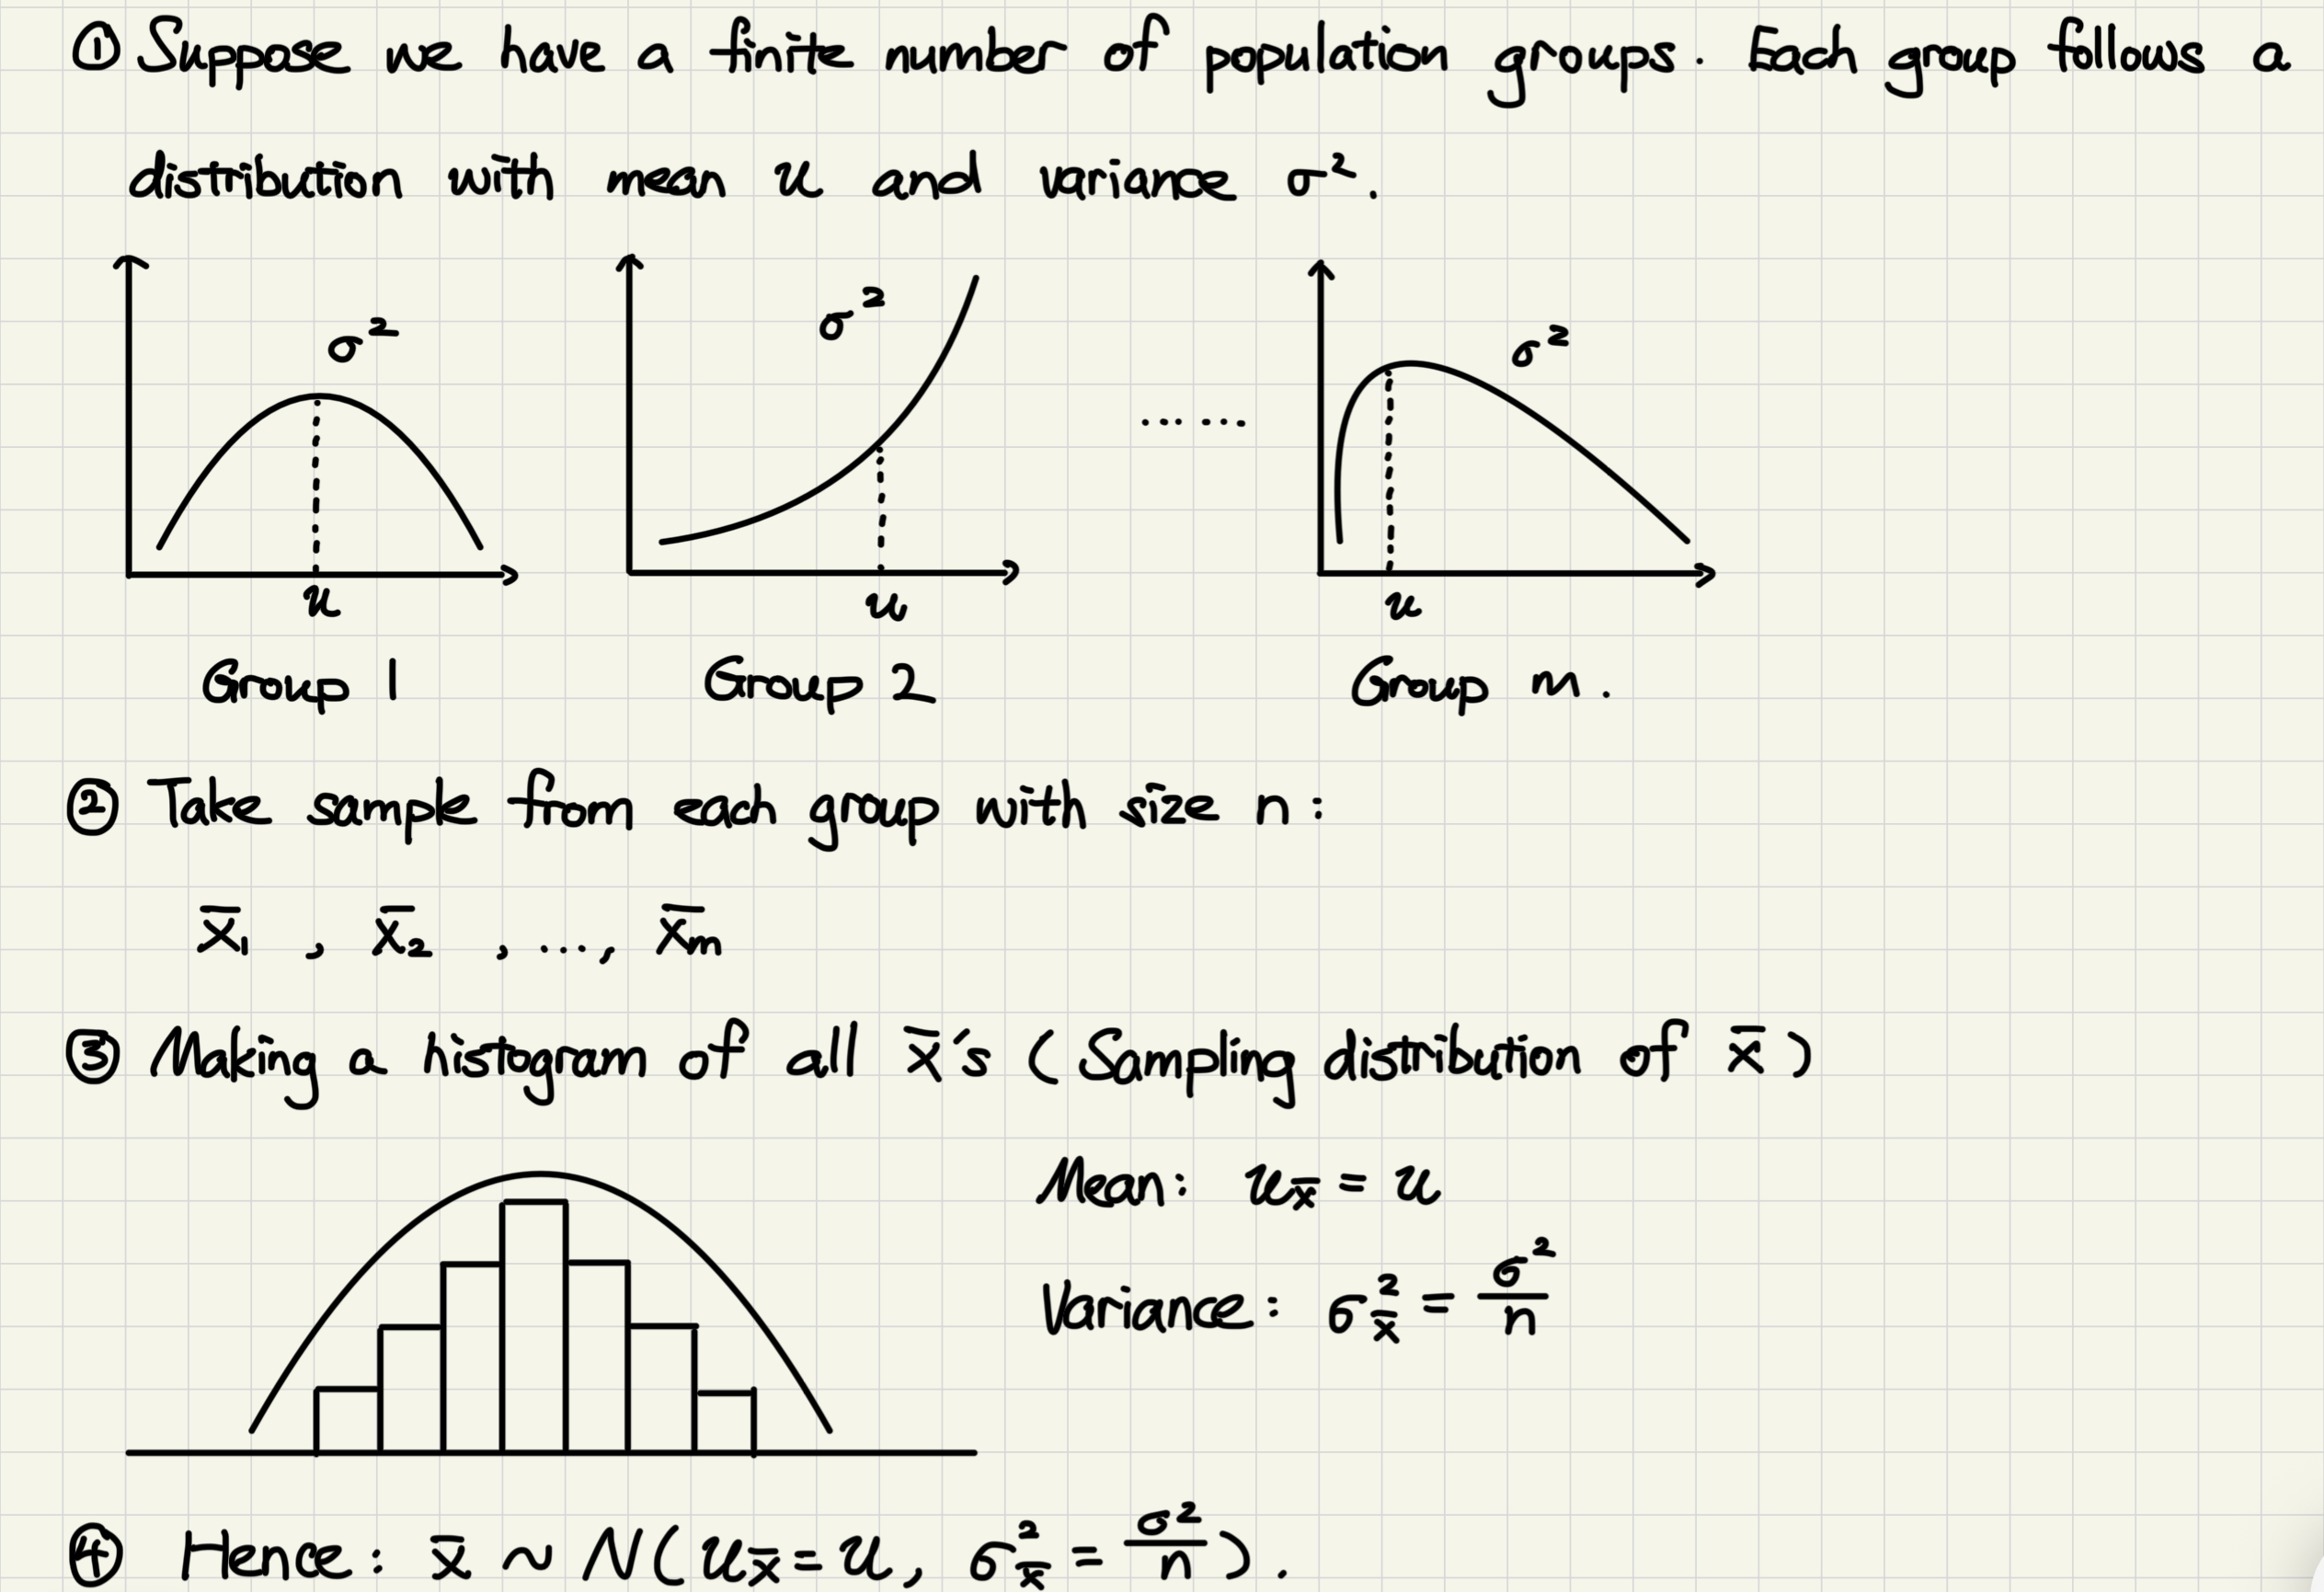
\includegraphics[scale=0.15]{Section3/Img3/CLT.jpg}
 \caption{Procedure of the Central Limit Theorem}
\end{figure}

\noindent
Now, let's begin with the proper definition of Central Limit Theorem.

\begin{definition}[Central Limit Theorem]
Let $X_1, X_2, ..., X_n$ be independent and identically distributed random variables with $E(X_i) = \mu$ and $Var(X_i) = \sigma^2 < \infty$. Then, we define the following: \[ U_{n} = \frac{\bar{X} - \mu}{(\frac{\sigma}{\sqrt{n}})} \sim N(\mu = 0, \sigma^2 = 1), \text{ where $\bar{X} = \frac{1}{n} \sum_{i =1}^{n}X_i$.}\]
Then the distribution function of $U_{n}$ converges to the standard Normal distribution function as $n \longrightarrow \infty$. That is, \[ \lim_{n\to\infty}P(U_n \le u) = \int_{\infty}^{u} \frac{1}{\sqrt{2\pi}} e^{-\frac{t^2}{2}}\,dt; \text{ for all u.}\]
\end{definition}

\noindent
For this course in particular, we do not need to pay that much attention to the proving part of the definition above. However, we use Central Limit Theorem to approximate distributions. Here are the two important approximations:

\begin{itemize}
	\item \[ \bar{X_n} \approx N(\mu, \frac{\sigma^2}{n});\]
	\item \[ T = \sum_{i = 1}^{n}X_i \approx N(n\mu, n\sigma^2).\]
\end{itemize}

\noindent
A reminder that the distribution of $U_n$ in definition $3.1$ and the two approximation of distribution above are extremely important in this course, until later chapters you may see some materials that are similar.
\setcounter{chapter}{3} % Makes this Chapter 4
\chapter{Normal Approximation to the Binomial Distribution}

\section{Introduction}

\begin{definition}[Statistic]
A \textit{statistic} is a function of the observable random variables in a sample and known constants.

Since statistics are functions of the random variables observed in a sample, they themselves are random variables. As such, all statistics have a corresponding probability distribution, which we refer to as their \textit{sampling distribution}.
\end{definition}
\begin{tcolorbox}[title=Review from STA256,
  colback=gray!5, 
  colframe=gray!40!black, 
  coltitle=black, 
  colbacktitle=gray!20,  % <- softer title bar
  fonttitle=\bfseries,
  sharp corners=south,
  breakable]


\textbf{Bernoulli Distribution:}

A Bernoulli trial is a single experiment with two outcomes:
\begin{itemize}
  \item Success: \( X = 1 \) with probability \( p \)
  \item Failure: \( X = 0 \) with probability \( 1 - p \)
\end{itemize}

\medskip

\begin{center}
\renewcommand{\arraystretch}{1.3}
\begin{tabular}{|c|c|c|}
\hline
\( X = x \) & 0 & 1 \\
\hline
\( P(X = x) \) & \( 1 - p \) & \( p \) \\
\hline
\end{tabular}
\end{center}

The probability mass function (PMF) is:
\[
f(x) = p^x (1 - p)^{1 - x}, \quad x \in \{0, 1\}
\]

\medskip

\textbf{Binomial Distribution:}

A binomial distribution arises from \( n \) independent Bernoulli trials. Let:
\[
X = \text{number of successes in } n \text{ trials}
\]
Then:
\[
X \sim \text{Binomial}(n, p)
\]

where:
\begin{itemize}
  \item Each trial results in either success (with probability \( p \)) or failure (with probability \( 1 - p \))
  \item \( X \in \{0, 1, \dots, n\} \)
\end{itemize}

The PMF is:
\[
P(X = x) = \binom{n}{x} p^x (1 - p)^{n - x}
\]

\medskip

\textbf{Moment Generating Function (MGF):}

The moment generating function (MGF) of a random variable \( X \) is defined as:
\[
M_X(t) = \mathbb{E}[e^{tX}]
\]
The MGF uniquely characterizes the distribution of \( X \) (if it exists in an open interval around 0), and it can be used to compute moments such as the mean and variance.


\end{tcolorbox}

\section{Bernoulli Distribution}
Bernoulli random variable is a discrete random variable that has exactly two possible outcomes which are either a \textbf{success} or a \textbf{failure}. An experiment in which there are exactly 2 outcomes (which are success or failure) is called a \textbf{Bernoulli trial}. \\
\vspace{1,0em} \\
When \( x = 1 \) we have a success and when \( x = 0 \) we have a failure. The term success and failure are relative to the problem being studied.

\begin{tcolorbox}[title=\textbf{TIP: ``success'' need not be something positive}, 
  colback=cyan!5, 
  colframe=cyan!40!black, 
  coltitle=black, 
  colbacktitle=cyan!10,
  fonttitle=\bfseries,
  sharp corners=south,
  breakable]

We chose to label a person who refuses to administer the worst shock a ``success'' and all others as ``failures''. However, we could just as easily have reversed these labels. The mathematical framework we will build does not depend on which outcome is labeled a success and which a failure, as long as we are consistent.

\end{tcolorbox}

\vspace{1,0em} 

Consider the random experiment of rolling a die once. Define the random variable:

\[
X_i =
\begin{cases}
1 & \text{if the } i\text{-th roll is a six}, \\
0 & \text{otherwise}
\end{cases}
\]

Then \( X_i \sim \text{Bernoulli}(p) \), where \( p = P(\text{rolling a six}) \). 
\begin{tcolorbox}[
  colback=yellow!10,
  colframe=yellow!10,
  boxrule=0pt,
  sharp corners=south,
  enhanced,
  breakable]

\textit{Let \( X \sim \text{Bernoulli}(p) \). The mass function of \( X \) is}

\[
P(X = x) = p^x (1 - p)^{1 - x}, \quad x = 0, 1
\]

\textit{where \( p \) represents the probability of success.}

\end{tcolorbox}




\begin{definition}[Mean and Variance of a Bernoulli Random Variable]
Let \( X \sim \text{Bernoulli}(p) \). The mean of \( X \) is
\[
E(X) = \mu = p
\]
and the variance of \( X \) is
\[
\text{Var}(X) = \sigma^2 = p(1 - p)
\]
\end{definition} 
\textit{To support the earlier result, we now provide a derivation of the mean, variance, and standard deviation of a Bernoulli random variable.}
\vspace{1,0em}  \\
Let \( X \) be a Bernoulli random variable with the probability of a success as \( p \). Then

\begin{align*}
E[X] = \mu & = \sum_{i=1}^{n} x_i \cdot P(X = x_i) \\
&= 0 \cdot P(X = 0) + 1 \cdot P(X = 1) \\
&= 0 \cdot (1 - p) + 1 \cdot p \\
&= p
\end{align*}
Similarly, the variance of \( X \) can be computed:

\begin{align*}
V(X) = \sigma^2 & = \sum_{i=1}^{k} (x_i - \mu)^2 \cdot P(X = x_i) \\
&= (0 - p)^2 \cdot P(X = 0) + (1 - p)^2 \cdot P(X = 1) \\
&= p^2 (1 - p) + (1 - p)^2 p \\
&= p(1 - p)
\end{align*}

The standard deviation is

\begin{align*}
\sigma & = \sqrt{\sigma^2} \\
            & = \sqrt{p(1 - p)}
\end{align*}




\section{Sampling Distribution of the Sum and MGF Derivation}

Consider determining the sampling distribution of the sample total:
\[
T_n = X_1 + X_2 + \dots + X_n
\]
Suppose \( X_i \overset{iid}{\sim} \text{Bernoulli}(p) \). Then the moment-generating function of \( T_n \) is:

\begin{align*}
M_{T_n}(t) &= \mathbb{E}[e^{t T_n}] \\
           &= \mathbb{E}\left[e^{t(X_1 + X_2 + \dots + X_n)}\right] \\
           &= \mathbb{E}\left[e^{tX_1} e^{tX_2} \dots e^{tX_n} \right] \quad \text{(independence)} \\
           &= \mathbb{E}[e^{tX_1}] \cdot \mathbb{E}[e^{tX_2}] \cdots \mathbb{E}[e^{tX_n}] \\
           &= M_{X_1}(t) \cdot M_{X_2}(t) \cdots M_{X_n}(t) \\
           &= \left[pe^t + (1 - p)\right]^n
\end{align*}


Since this is the MGF of a binomial random variable with parameters \( n \) and \( p \), we conclude:

\[
T_n \sim \text{Binomial}(n, p)
\]
\medskip
\begin{tcolorbox}[title=Example: Binomial Distribution from Die Rolls,
  colback=blue!5, colframe=blue!40!black, coltitle=black,
  colbacktitle=blue!10!white, fonttitle=\bfseries, breakable]

We can think of rolling a die \( n \) times as an example of the binomial setting. Each roll gives either a six (a “success”) or a number different from six (a “failure”).

Knowing the outcome of one roll doesn’t tell us anything about the others, so the \( n \) rolls are independent.

If we call a six a success, then:
\begin{itemize}
  \item The probability of success on each trial is \( p = P(\text{rolling a six}) = \frac{1}{6} \)
  \item The probability of failure is \( 1 - p = \frac{5}{6} \)
\end{itemize}

Let \( Y \) be the number of sixes rolled in \( n \) trials. Then \( Y \sim \text{Binomial}(n, p) \), and the distribution of \( Y \) is called a \textbf{binomial distribution}.
\end{tcolorbox}


\section{Binomial Distribution} % or \section{4.4 Binomial Distribution} if numbering manually

In section 4.2 we learnt about Bernoulli random variables in which we were interested in the outcome of just a single trial. A \textbf{binomial random variable} is a generalization of several independent Bernoulli trials. Instead of performing just a single Bernoulli trial and observing whether we have a success or not, we are now performing several Bernoulli trials and observing whether we have a certain number of successes and failures. The \textbf{binomial distribution} describes the probability of having exactly \( k \) successes in \( n \) independent Bernoulli trials with probability of a success \( p \). \\
\begin{tcolorbox}[
  colback=yellow!10,
  colframe=yellow!10,
  boxrule=0pt,
  sharp corners=south,
  enhanced,
  breakable]

\textit{Let \( X \sim \text{Bin}(n, p) \). The probability of observing \( x \) successes in these \( n \) independent trials is given by}

\[
P(X = x) = \binom{n}{x} p^x (1 - p)^{n - x}
\]

\textit{where}
\begin{itemize}
  \item \( n \) represents the number of trials,
  \item \( x \) represents the number of successes,
  \item \( p \) represents the probability of success on any given trial,
\end{itemize}

\[
\binom{n}{x} = \frac{n!}{x!(n - x)!} \quad \text{is the binomial coefficient.}
\]

\end{tcolorbox}

\begin{definition}[Mean and Variance of a Binomial Random Variable]
Let \( X \sim \text{Bin}(n, p) \). The mean of \( X \) is
\[
E(X) = \mu = np
\]
\textit{and the variance of \( X \) is}
\[
\text{Var}(X) = \sigma^2 = np(1 - p)
\]
\end{definition}



\subsection{Visualizing the PMF of Binomial Distributions}

\noindent\textbf{R code:}
\begin{tcolorbox}[colback=gray!10, colframe=black!45, arc=2mm]
\begin{verbatim}
## Pmf of Binomial with n=10 and p=1/6.

x <- seq(0, 10, by=1)
y <- dbinom(x, 10, 1/6)

plot(x, y, type="p", col="blue", pch=19)
\end{verbatim}
\end{tcolorbox}


\textbf{Probability Mass Functions (PMFs) for increasing \(n\):}

\vspace{0.5em}

The following plots display the probability mass functions (PMFs) for a binomial distribution with \( p = \frac{1}{6} \) and increasing values of \( n \). As \( n \) increases, the binomial distribution begins to resemble a normal distribution.


\begin{figure}[h!]
  \centering
 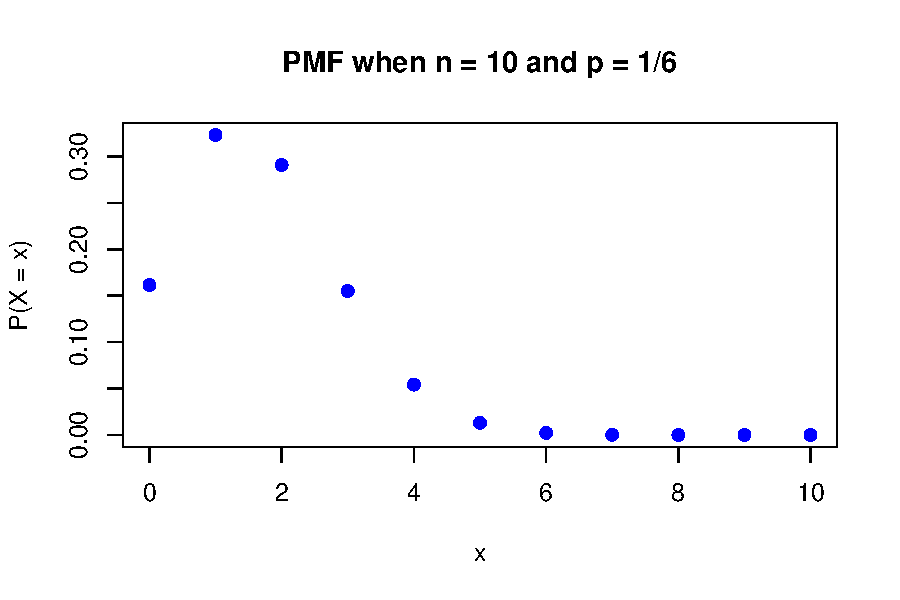
\includegraphics[width=0.8\textwidth]{Section4/images/pmf_plot.pdf}
 \vspace{-10pt} % ⬅️ reduces space between figure and caption
\captionsetup{skip=0pt} % Decreases space between figure and caption
 \caption{PMF of Binomial distribution with \(n = 10\) and \(p = \frac{1}{6}\).}
\end{figure}

\begin{figure}[h!]
  \centering
  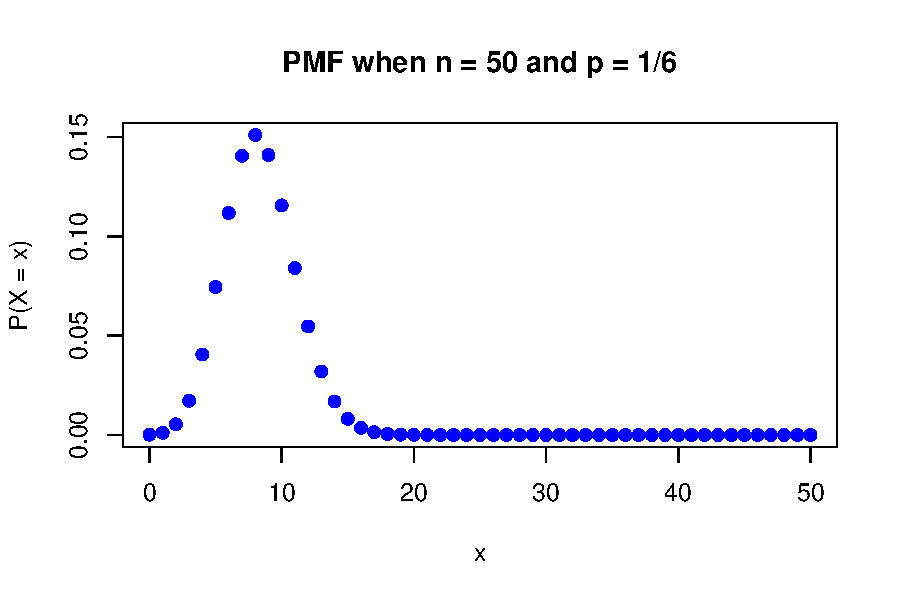
\includegraphics[width=0.8\textwidth]{Section4/images/pmf_n50.pdf}
  \vspace{-10pt} % ⬅️ reduces space between figure and caption
  \captionsetup{skip=0pt} % Decreases space between figure and caption
  \caption{PMF of Binomial distribution with \(n = 50\) and \(p = \frac{1}{6}\).}
\end{figure}

\begin{figure}[h!]
  \centering
  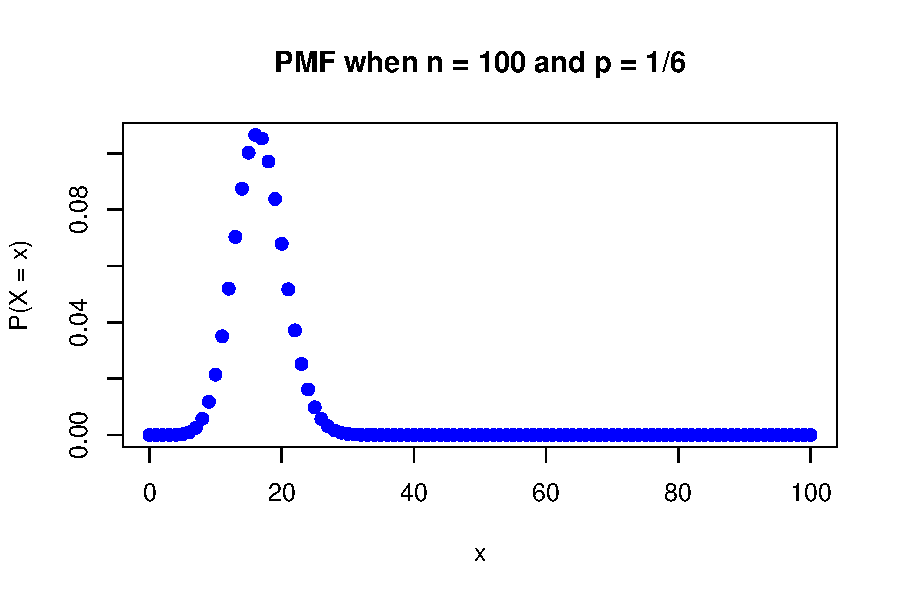
\includegraphics[width=0.8\textwidth]{Section4/images/pmf_n100.pdf}
  \vspace{-10pt} % ⬅️ reduces space between figure and caption
\captionsetup{skip=0pt} % Decreases space between figure and caption
  \caption{PMF of Binomial distribution with \(n = 100\) and \(p = \frac{1}{6}\).}
\end{figure}

\begin{figure}[h!]
  \centering
  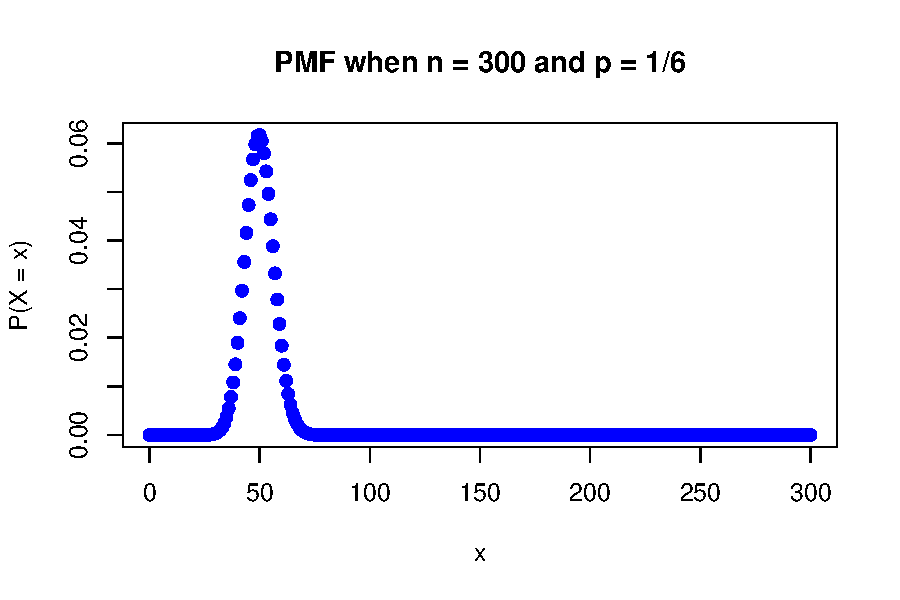
\includegraphics[width=0.8\textwidth]{Section4/images/pmf_n300.pdf}
  \vspace{-10pt} % ⬅️ reduces space between figure and caption
\captionsetup{skip=0pt} % Decreases space between figure and caption
  \caption{PMF of Binomial distribution with \(n = 300\) and \(p = \frac{1}{6}\).}
\end{figure}
% 🔁 Force figures to be placed before moving on
\clearpage


\section{Sampling Distribution of a Sample Proportion and the Normal Approximation}
When studying categorical data, we are often interested not just in individual outcomes, but in the proportion of successes observed in a sample. Understanding how this proportion behaves across repeated samples is crucial for making inferences about a population. In this section, we explore the sampling distribution of a sample proportion and how it can be approximated by a normal distribution under certain conditions.\\
\vspace{0.5em}

Draw a \textit{Simple Random Sample (SRS)} of size \( n \) from a large population that contains proportion \( p \) of “successes”. Let \( \hat{p} \) be the \textbf{\textit{sample proportion}} of successes:

\[
\hat{p} = \frac{\text{number of successes in the sample}}{n}
\]

Then:

\begin{itemize}
  \item The \textbf{mean} of the sampling distribution of \( \hat{p} \) is \( p \).
  \item The \textbf{standard deviation} of the sampling distribution is \( \sqrt{ \frac{p(1 - p)}{n} } \).
\end{itemize}


\begin{figure}[h!]
  \centering
  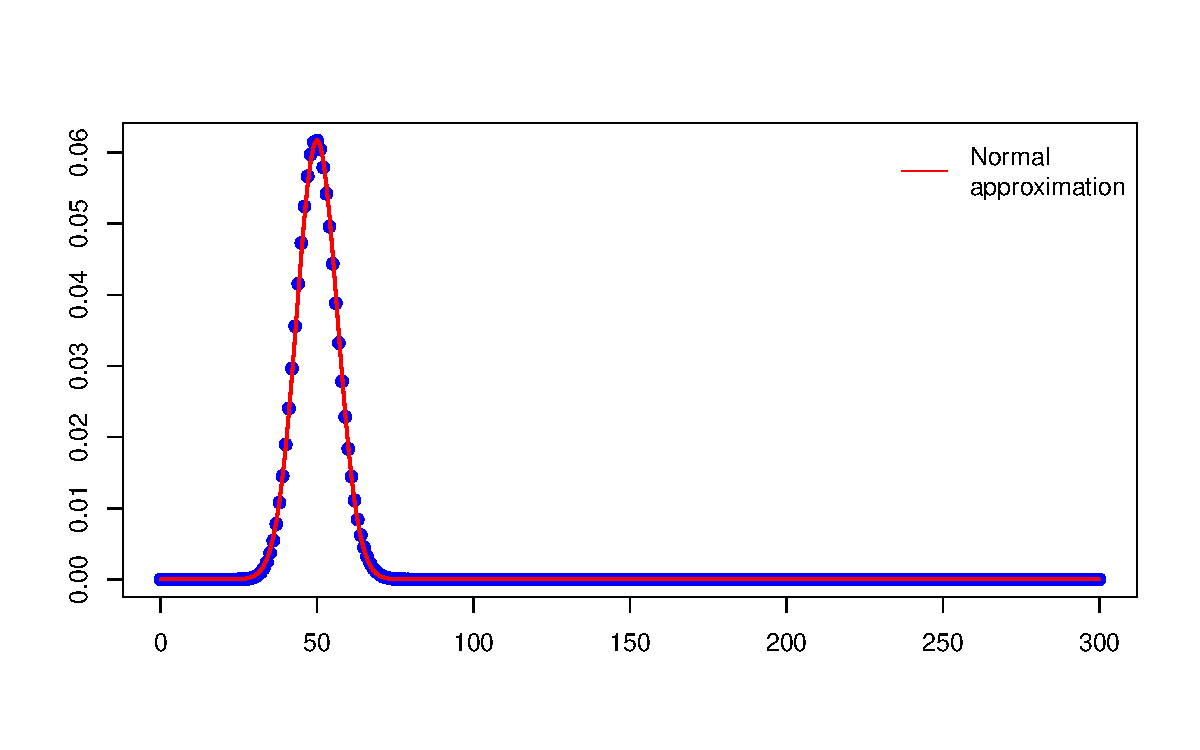
\includegraphics[width=0.9\textwidth]{Section4/images/binomial_normal.pdf}
  \vspace{-10pt} % ⬅️ reduces space between figure and caption
  \captionsetup{skip=0pt} % Decreases space between figure and caption
  \caption{Binomial distribution with \(n = 300\), \(p = \frac{1}{6}\) and its Normal approximation.}
\end{figure}


According to the Central Limit Theorem (CLT), the sampling distribution of a sample proportion becomes approximately normal as the sample size increases.

That is:
\[
\hat{p} \sim \mathcal{N}\left(p, \sqrt{\frac{p(1 - p)}{n}}\right)
\]

This approximation is most accurate when both \( np \geq 10 \) and \( n(1 - p) \geq 10 \).

These are called the \textbf{success-failure conditions}.

\medskip

\textit{Key Point:} When the success-failure conditions are met, the normal approximation to the sampling distribution of \( \hat{p} \) can be used for probability calculations.
\subsection*{Conditions for Using the Normal Approximation}

\vspace{0.5em}

Suppose \( X \sim \text{Binomial}(n, p) \). Then:

\[
\mu = np, \quad \sigma^2 = np(1 - p)
\]

\medskip

\textbf{Binomial probabilities can be approximated by the normal distribution:}
\[
X \approx \mathcal{N}(np, \, np(1 - p))
\]

This approximation is \textit{useful for large \( n \)} and valid under the following conditions:

\begin{tcolorbox}[title=Standard Conditions,
  colback=blue!5, 
  colframe=blue!50!black, 
  coltitle=black,
  colbacktitle=blue!20, % ← LIGHTER blue for the title bar
  fonttitle=\bfseries,
  sharp corners=south,
  boxrule=0.5pt,
  enhanced,
  width=\textwidth,
  breakable]
The binomial setting holds (i.e., independent trials, fixed \( n \), same probability \( p \)) and

\[
np \geq 10 \quad \text{and} \quad np(1 - p) \geq 10
\]
\end{tcolorbox}

\vspace{0.5em}

Alternatively, a more conservative criterion for using the normal approximation is:
\[
n > 9 \cdot \left( \frac{\max(p, \, 1 - p)}{\min(p, \, 1 - p)} \right)
\]

\medskip

These ensure that the binomial distribution is sufficiently symmetric and smooth to approximate with the normal distribution.

\medskip
We derive the sampling distribution of \( \hat{p} \) using properties of the Bernoulli distribution.

\subsection*{Bernoulli Distribution (Binomial with $n = 1$)}

\[
X_i =
\begin{cases}
1 & \text{if the $i$-th roll is a six} \\
0 & \text{otherwise}
\end{cases}
\]

\[
\mu = \mathbb{E}(X_i) = p, \quad \sigma^2 = \mathrm{Var}(X_i) = p(1 - p)
\]

Let $\hat{p}$ be our estimate of $p$. Note that $\hat{p} = \frac{1}{n} \sum_{i=1}^{n} X_i = \bar{X}$.
Let $\hat{p} = \frac{\text{\# successes } (X)}{\text{sample size } (n)}$

Recall that for $X \sim \text{Binomial}(n, p)$:
\[
X \overset{\cdot}{\sim} \mathcal{N}(np, np(1 - p))
\]

Let $\hat{p} = \frac{X}{n}$

\paragraph*{Mean of $\hat{p}$:}

\[
\mathbb{E}(\hat{p}) = \mathbb{E} \left( \frac{X}{n} \right) = \frac{1}{n} \cdot \mathbb{E}(X) = \frac{1}{n} \cdot np = p
\]

\paragraph*{Variance of $\hat{p}$:}

\[
\mathrm{Var}(\hat{p}) = \mathrm{Var} \left( \frac{X}{n} \right) = \frac{1}{n^2} \cdot \mathrm{Var}(X) = \frac{1}{n^2} \cdot np(1 - p) = \frac{p(1 - p)}{n}
\]

By the Central Limit Theorem (CLT), for sufficiently large $n$:
\[
\hat{p} \sim \mathcal{N} \left( p, \frac{p(1 - p)}{n} \right)
\]

\paragraph*{Standardization of $\hat{p}$:}
\[
Z = \frac{\hat{p} - p}{\sqrt{ \frac{p(1 - p)}{n} }}
\]

If $n$ is large, then by the Central Limit Theorem:
\[
\bar{X} \approx \mathcal{N} \left( \mu, \frac{\sigma}{\sqrt{n}} \right)
\quad \Rightarrow \quad
\hat{p} \sim \mathcal{N} \left( p, \sqrt{\frac{p(1 - p)}{n}} \right)
\]
\begin{example}[Normal Approximation for Proportions]
In the last election, a state representative received 52\% of the votes cast. One year after the election, the representative organized a survey that asked a random sample of 300 people whether they would vote for him in the next election. If we assume that his popularity has not changed, what is the probability that more than half the sample would vote for him?


\vspace{1em}
\subsubsection*{Solution 1 (using Normal Approximation)}

We want to determine the probability that the sample proportion is greater than 50\%. In other words, we want to find $P(\hat{p} > 0.50)$.

We know that the sample proportion $\hat{p}$ is roughly Normally distributed with mean $p = 0.52$ and standard deviation
\begin{align*}
\sqrt{p(1 - p)/n} & =  \sqrt{(0.52)(0.48)/300} = 0.0288. \\
\end{align*}
\begin{align*}
Thus, we calculate \\
P(\hat{p} > 0.50) & = P\left( \frac{\hat{p} - p}{\sqrt{p(1-p)/n}} > \frac{0.50 - 0.52}{0.0288} \right) \\
&= P(Z > -0.69) = 1 - P(Z < -0.69) \quad \text{(Z is symmetric)} \\
&= P(Z > -0.69) = 1 - P(Z > 0.69) \\
&= 1 - 0.2451 = 0.7549.
\end{align*}

If we assume that the level of support remains at 52\%, the probability that more than half the sample of 300 people would vote for the representative is 0.7549.\par
\vspace{0.5em}
\noindent\textbf{R code (Normal Approximation):}
\begin{tcolorbox}[colback=gray!10, colframe=black!45, arc=2mm]
\begin{verbatim}
1 - pnorm(0.50, mean = 0.52, sd = 0.0288)
## [1] 0.7562982
\end{verbatim}
\end{tcolorbox}

Recall that, \texttt{pnorm} will give you the area to the left of 0.50, for a Normal distribution with mean 0.52 and standard deviation 0.0288.
\subsubsection*{Solution 2 (using Binomial)}

We want to determine the probability that the sample proportion is greater than 50\%. In other words, we want to find $P(\hat{p} > 0.50)$. We know that 
$n = 300$ and $p = 0.52$. \\
Thus, we calculate
\begin{align*}
P(\hat{p} > 0.50) &= P\left(\frac{\sum_{i=1}^{n} x_i}{n} > 0.50\right) \\
&= P\left(\sum_{i=1}^{300} x_i > 150\right) \\
&= 1 - P\left(\sum_{i=1}^{300} x_i \leq 150\right) \\
&\text{(it can be shown that } Y = \sum_{i=1}^{300} x_i \text{ has a Binomial distribution with} \\
&n = 300 \text{ and } p = 0.52\text{)} \\
&= 1 - F_Y(150)
\end{align*}

\vspace{0.5em}
\noindent\textbf{R code (using Binomial distribution):}
\begin{tcolorbox}[colback=gray!10, colframe=black!45, arc=2mm]
\begin{verbatim}
1- pbinom(150, size = 300, prob = 0.52);
## [1] 0.7375949
\end{verbatim}
\end{tcolorbox}
Recall that, \texttt{pbinom} will give you the CDF at 150, for a Binomial distribution with $n = 300$ and $p = 0.52$.

\subsection*{Solution 3 (using continuity correction)}


We have that $n = 300$ and $p = 0.52$.
Thus, we calculate
\begin{align*}
P(\hat{p} > 0.50) &= P\left( \frac{\sum_{i=1}^{n} x_i}{n} > 0.50 \right) \\
&= P\left( \sum_{i=1}^{300} x_i > 150 \right) \\
&= 1 - P\left( \sum_{i=1}^{300} x_i \leq 150 \right) \\
&\text{(it can be shown that } Y = \sum_{i=1}^{300} x_i \text{ has a Binomial distribution with} \\
&n = 300 \text{ and } p = 0.52\text{)}. \\
&\approx 1 - P\left( \sum_{i=1}^{300} x_i \leq 150.5 \right) \quad \text{(continuity correction)} \\
&= 1 - P\left( \frac{\sum_{i=1}^{300} x_i}{n} \leq \frac{150.5}{300} \right) \\
&= 1 - P(\hat{p} \leq 0.5017) \\
&= 1 - P\left( Z \leq -0.6354 \right) \quad \text{(Why?)}
\end{align*}
\noindent\textbf{R code (Normal approximation with continuity correction):}
\begin{tcolorbox}[colback=gray!10, colframe=black!45, arc=2mm]
\begin{verbatim}
1 - pnorm(0.5017, mean = 0.52, sd = 0.0288)
## [1] 0.7374216
\end{verbatim}
\end{tcolorbox}

Recall that, \texttt{pnorm} will give you the area to the left of 0.5017, for a Normal distribution with mean 0.52 and standard deviation 0.0288.
\end{example}

\section{Normal Approximation to Binomial}

Let $X = \sum_{i=1}^{n} Y_i$ where $Y_1, Y_2, \ldots, Y_n$ are iid Bernoulli random variables. Note that $X = n\hat{p}$.

\begin{enumerate}
    \item $n\hat{p}$ is approximately Normally distributed provided that $np \geq 10$ and $n(1 - p) \geq 10$.

    \item Another criterion is that the Normal approximation is adequate if
    \[
    n > 9 \left( \frac{\text{larger of $p$ and $q$}}{\text{smaller of $p$ and $q$}} \right)
    \]

    \item The expected value: $E(\hat{p}) = np$.

    \item The variance: $V(\hat{p}) = np(1 - p) = npq$.
\end{enumerate}


\section{Continuity Correction}
The normal distribution is continuous, while the binomial distribution is discrete. When we approximate a binomial probability using the normal distribution, this mismatch can lead to inaccuracy—especially near the boundaries of discrete values. A continuity correction improves the approximation by adjusting for this difference. In this section, we explore how and why this correction is applied. \\
\subsection*{Continuity Correction Table}

%\begin{table}[h!]
%\centering
%\rowcolors{2}{gray!15}{white} % Alternating row colors
%\begin{tabular}{@{}lll@{}}
%\toprule
%\textbf{Binomial Probability}        & \textbf{Continuity Correction}                & \textbf{Normal Approximation}                                                                 \\ \midrule
%$\displaystyle P(X = x)$             & $\displaystyle P(x - 0.5 \leq X \leq x + 0.5)$ & $\displaystyle P\left(\frac{x - 0.5 - \mu}{\sigma} \leq Z \leq \frac{x + 0.5 - \mu}{\sigma}\right)$ \\[1.00em] 
%$\displaystyle P(X \leq x)$          & $\displaystyle P(X \leq x + 0.5)$              & $\displaystyle P\left(Z \leq \frac{x + 0.5 - \mu}{\sigma}\right)$                                 \\[1.00em] 
%$\displaystyle P(X < x)$             & $\displaystyle P(X \leq x - 0.5)$              & $\displaystyle P\left(Z \leq \frac{x - 0.5 - \mu}{\sigma}\right)$                                 \\[1.00em] 
%$\displaystyle P(X \geq x)$          & $\displaystyle P(X \geq x - 0.5)$              & $\displaystyle P\left(Z \geq \frac{x - 0.5 - \mu}{\sigma}\right)$                                 \\[1.00em] 
%$\displaystyle P(X > x)$             & $\displaystyle P(X \geq x + 0.5)$              & $\displaystyle P\left(Z \geq \frac{x + 0.5 - \mu}{\sigma}\right)$                                 \\[1.00em] 
%$\displaystyle P(a \leq X \leq b)$   & $\displaystyle P(a - 0.5 \leq X \leq b + 0.5)$ & $\displaystyle P\left(\frac{a - 0.5 - \mu}{\sigma} \leq Z \leq \frac{b + 0.5 - \mu}{\sigma}\right)$ \\ \bottomrule
%\end{tabular}
%\end{table}


\begin{center}
\renewcommand{\arraystretch}{1.3}
\begin{tabular}{| l | c | c | c | c | }
\hline
\textbf{Binomial Probability}        & \textbf{Continuity Correction}                & \textbf{Normal Approximation}\\                                                             
\hline
\hfill	&	&\\
$\displaystyle P(X = x)$             & $\displaystyle P(x - 0.5 \leq X \leq x + 0.5)$ & $\displaystyle P\left(\frac{x - 0.5 - \mu}{\sigma} \leq Z \leq \frac{x + 0.5 - \mu}{\sigma}\right)$ \\[1.00em] 
\hline
\hfill	&	&\\
$\displaystyle P(X \leq x)$          & $\displaystyle P(X \leq x + 0.5)$              & $\displaystyle P\left(Z \leq \frac{x + 0.5 - \mu}{\sigma}\right)$\\[0.75em]  
\hline
\hfill	&	&\\
$\displaystyle P(X < x)$             & $\displaystyle P(X \leq x - 0.5)$              & $\displaystyle P\left(Z \leq \frac{x - 0.5 - \mu}{\sigma}\right)$\\[0.75em] 
\hline
\hfill	&	&\\
$\displaystyle P(X \geq x)$          & $\displaystyle P(X \geq x - 0.5)$              & $\displaystyle P\left(Z \geq \frac{x - 0.5 - \mu}{\sigma}\right)$\\[0.75em]
\hline
\hfill	&	&\\
$\displaystyle P(X > x)$             & $\displaystyle P(X \geq x + 0.5)$              & $\displaystyle P\left(Z \geq \frac{x + 0.5 - \mu}{\sigma}\right)$\\[0.75em] 
\hline
\hfill	&	&\\
$\displaystyle P(a \leq X \leq b)$   & $\displaystyle P(a - 0.5 \leq X \leq b + 0.5)$ & $\displaystyle P\left(\frac{a - 0.5 - \mu}{\sigma} \leq Z \leq \frac{b + 0.5 - \mu}{\sigma}\right)$ \\
\hfill	&	&\\
\hline
\end{tabular}
\end{center}

\vspace{0.5em} 
Suppose that $Y$ has a Binomial distribution with $n = 20$ and $p = 0.4$. We will find the exact probabilities that $Y \leq y$ and compare these to the corresponding values found by using two Normal approximations. One of them, when $X$ is Normally distributed with $\mu_X = np$ and $\sigma_X = \sqrt{np(1 - p)}$.
\vspace{1em}
The other one, $W$, a shifted version of $X$.

\vspace{1em}

For example,
\[
P(Y \leq 8) = 0.5955987
\]

As previously stated, we can think of $Y$ as having approximately the same distribution as $X$.
\[
P(Y \leq 8) \approx P(X \leq 8)
= P\left[ \frac{X - np}{\sqrt{np(1 - p)}} \leq \frac{8 - 8}{\sqrt{20(0.4)(0.6)}} \right]
= P(Z \leq 0) = 0.5
\]

\vspace{1em}

\[
P(Y \leq 8) \approx P(W \leq 8.5)
= P\left[ \frac{W - np}{\sqrt{np(1 - p)}} \leq \frac{8.5 - 8}{\sqrt{20(0.4)(0.6)}} \right]
= P(Z \leq 0.2282) = 0.5902615
\]

\vspace{1em}

\begin{example}

Fifty-one percent of adults in the U. S. whose New Year’s resolution was to exercise more achieved their resolution. You randomly select 65 adults in the U. S. whose resolution was to exercise more and ask each if he or she achieved that resolution. What is the probability that exactly forty of them respond yes?\\

We are given that $p = 0.51$, $n = 65$, and we want to find $P(X = 40)$ where $X \sim Binomial(n = 65, p = 0.51)$.\\

\textbf{Use Normal Approximation}
\vspace{0.5 em}
We use normal approximation to the binomial. First, compute the mean and standard deviation:
\begin{align*}
\mu &= np = 65 \times 0.51 = 33.15 \\
\sigma^2 &= np(1-p) = 65 \times 0.51 \times 0.49 = 16.485 \\
\sigma &= \sqrt{16.485} \approx 4.06
\end{align*}


We apply continuity correction:
\[
P(X = 40) = P(39.5 \leq X \leq 40.5)
\]

\[
= P\left(\frac{39.5 - 33.15}{4.06} \leq Z \leq \frac{40.5 - 33.15}{4.06}\right) = P(1.56 \leq Z \leq 1.81)
\]

From the standard normal table:
\[
= P(Z \leq 1.81) - P(Z \leq 1.56) = 0.0594 - 0.0352 = 0.0242
\]

So the approximate probability is:
\[
P(X = 40) \approx 0.0242
\]
\end{example}







%\chapter{Law of Large Numbers}
\section{Convergence in Probability}

\vspace{1em}


\begin{definition}[Convergence in Probability]
The sequence of random variables \( X_1, X_2, X_3, \ldots, X_n, \ldots \) is said to \textbf{converge in probability} to the constant \( c \), if for every \( \epsilon > 0 \),
\[
\lim_{n \to \infty} P\left( |X_n - c| \leq \epsilon \right) = 1
\]
or equivalently,
\[
\lim_{n \to \infty} P\left( |X_n - c| > \epsilon \right) = 0
\]

\noindent \textbf{Notation:} \( X_n \xrightarrow{P} c \)
\end{definition}

\vspace{1em}

This concept plays a key role in the Law of Large Numbers, where the sample mean of independent and identically distributed random variables converges in probability to the population mean as the sample size grows.

\vspace{2em}

\begin{definition}[Chebyshev’s Inequality]
Let \( X \) be a random variable with finite mean \( \mu \) and variance \( \sigma^2 \). Then, for any \( k > 0 \),
\[
P\left( |X - \mu| \geq k \right) \leq \frac{\sigma^2}{k^2}
\]

\textit{Using complements:}
\[
P\left( |X - \mu| < k \right) \geq 1 - \frac{\sigma^2}{k^2}
\]
\end{definition}

\newpage

\section{Weak Law of Large Numbers (WLLN)}

\begin{definition}[Weak Law of Large Numbers (WLLN)]
Let \( X_1, X_2, \ldots \) be a sequence of independent and identically distributed random variables, each having finite mean \( E(X_i) = \mu \) and variance \( \mathrm{Var}(X_i) = \sigma^2 \). Then, for any \( \epsilon > 0 \),
\[
P\left( \left| \frac{X_1 + X_2 + \cdots + X_n}{n} - \mu \right| \geq \epsilon \right) \to 0 \quad \text{as } n \to \infty
\]

\noindent\textbf{Notation:} \( \bar{X}_n \xrightarrow{P} \mu \)
\end{definition}
\subsection*{Proof of the Weak Law of Large Numbers (WLLN)}

We aim to show that for every \( \epsilon > 0 \),
\[
\lim_{n \to \infty} P\left( \left| \bar{X}_n - \mu \right| > \epsilon \right) = 0
\]
where \( \bar{X}_n \) is the sample mean of \( n \) independent and identically distributed (i.i.d.) random variables with
\[
E(X_i) = \mu, \quad \text{and} \quad \mathrm{Var}(X_i) = \sigma^2.
\]

Let
\[
\bar{X}_n = \frac{1}{n} \sum_{i=1}^{n} X_i.
\]

By the Central Limit Theorem (CLT), we know that
\[
\bar{X}_n \sim \mathcal{N} \left( \mu, \frac{\sigma^2}{n} \right).
\]

Now, applying \textbf{Chebyshev’s Inequality}, which states that for any random variable \( X \) with mean \( \mu \) and variance \( \sigma^2 \),
\[
P\left( |X - \mu| > k \right) \leq \frac{\sigma^2}{k^2} \quad \text{for } k > 0,
\]
to \( \bar{X}_n \), we set \( k = \epsilon \), and obtain:
\[
P\left( \left| \bar{X}_n - \mu \right| > \epsilon \right) \leq \frac{\mathrm{Var}(\bar{X}_n)}{\epsilon^2} = \frac{\sigma^2 / n}{\epsilon^2} = \frac{\sigma^2}{n \epsilon^2}.
\]

Taking the limit as \( n \to \infty \), we have:
\[
\lim_{n \to \infty} P\left( \left| \bar{X}_n - \mu \right| > \epsilon \right) \leq \lim_{n \to \infty} \frac{\sigma^2}{n \epsilon^2} = 0.
\]

Since probabilities are always non-negative, we conclude:
\[
\lim_{n \to \infty} P\left( \left| \bar{X}_n - \mu \right| > \epsilon \right) = 0.
\]

By the definition of convergence in probability,
\[
\bar{X}_n \xrightarrow{P} \mu.
\]
\qed
\begin{example}[Poisson Convergence via WLLN]

Let \( X_i \), for \( i = 1, 2, 3, \ldots \), be independent Poisson random variables with rate parameter \( \lambda = 3 \). Prove that:
\[
\bar{X}_n \xrightarrow{P} 3
\]

\textbf{Properties of Poisson Distribution:}
\[
E(X_i) = \lambda, \quad \mathrm{Var}(X_i) = \lambda
\]
In this case, \( \lambda = 3 \), so:
\[
E(X_i) = \mathrm{Var}(X_i) = 3
\]

\textbf{Proof:}

We know:
\[
E\left( \frac{X_1 + X_2 + \cdots + X_n}{n} \right) = 3, \quad \text{and} \quad
\mathrm{Var}\left( \frac{X_1 + X_2 + \cdots + X_n}{n} \right) = \frac{3}{n}
\]

Applying Chebyshev’s Inequality:
\[
P\left( \left| \frac{X_1 + X_2 + \cdots + X_n}{n} - 3 \right| \geq \epsilon \right) \leq \frac{3}{n \epsilon^2}
\]

Taking the limit as \( n \to \infty \):
\[
P\left( \left| \frac{X_1 + X_2 + \cdots + X_n}{n} - 3 \right| \geq \epsilon \right) \to 0
\]

\textbf{Conclusion:}
\[
\bar{X}_n \xrightarrow{P} 3
\]
\end{example}
\begin{figure}[H]
  \centering
  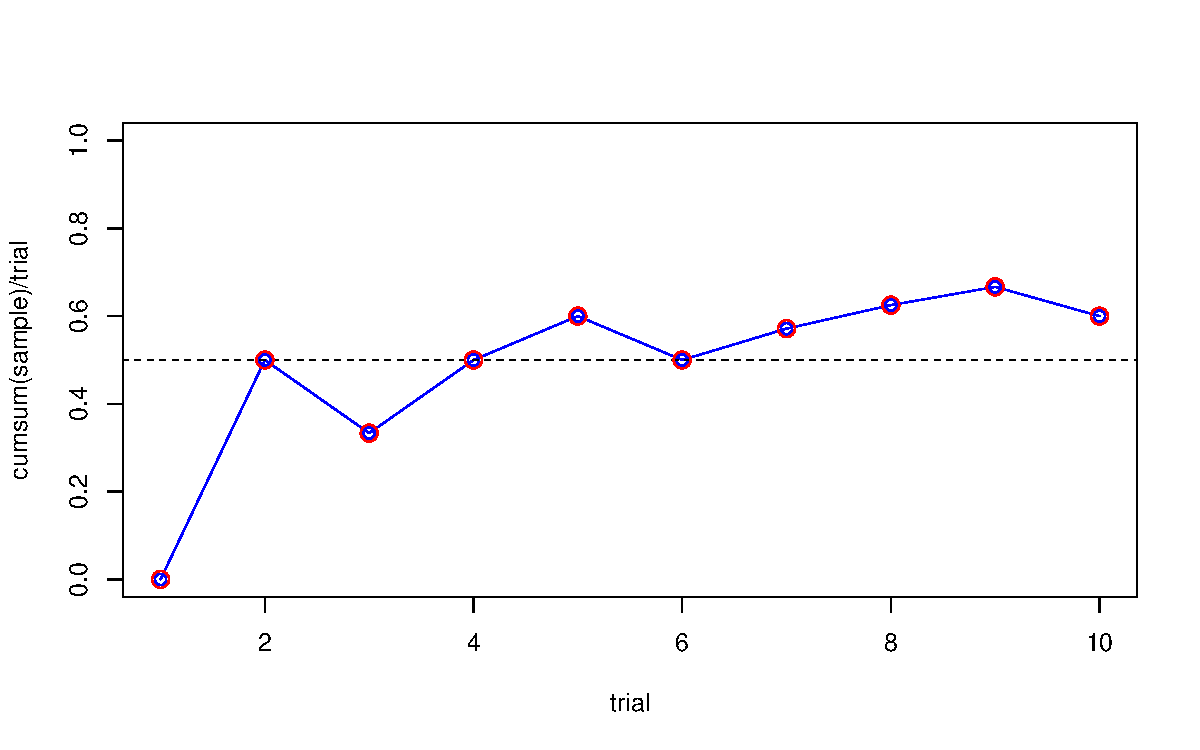
\includegraphics[width=0.72\textwidth]{Section5/images/simulation_plot.pdf}
  \caption{Simulation of running sample mean of Bernoulli(\(p = 0.5\)) trials over time.}
\end{figure}

{\color{gray} \textbf{R Simulation Code (Single Sample Path)}}

\begin{verbatim}
n = 10
trial = seq(1, n, by = 1)
sample = rbinom(n, 1, 1/2)

plot(trial, cumsum(sample)/trial, type = "l", ylim = c(0,1), col = "blue")
points(trial, cumsum(sample)/trial, col = "red")
abline(h = 0.5, lty = 2, col = "black")
\end{verbatim}

\begin{figure}[H]
  \centering
  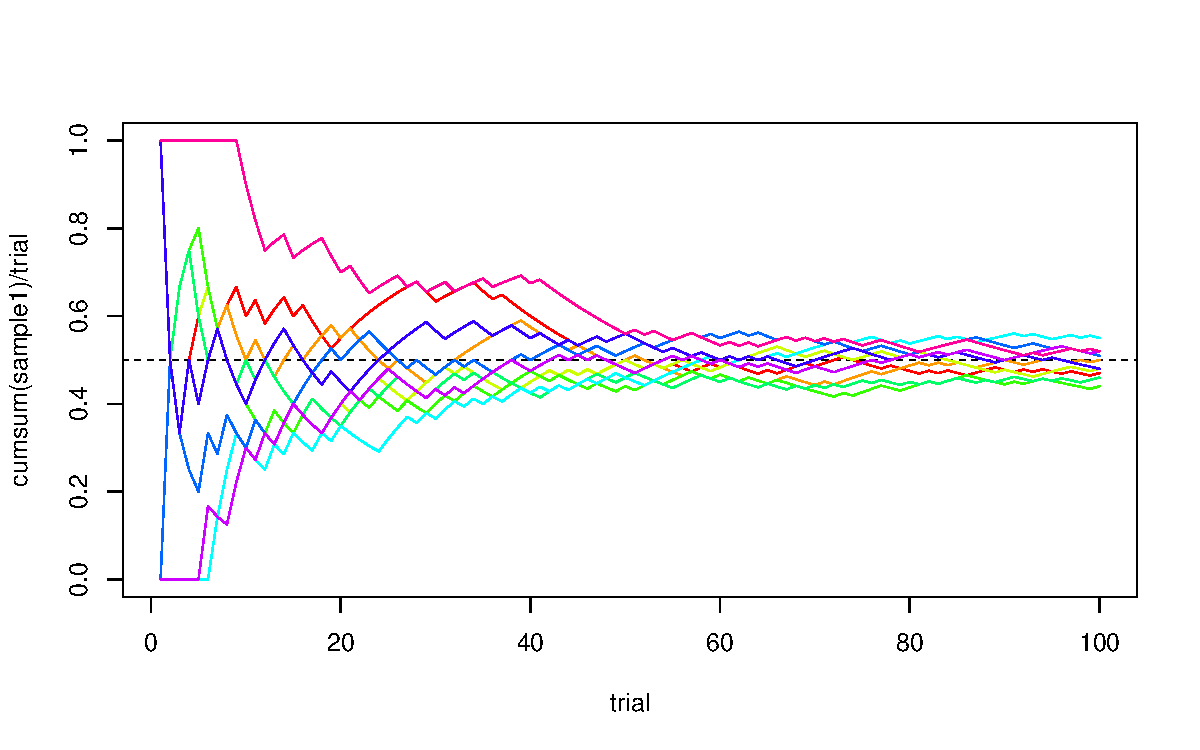
\includegraphics[width=0.72\textwidth]{Section5/images/simulation_multi.pdf}
  \caption{Simulation of 10 running sample means of Bernoulli(\(p = 0.5\)) trials converging over 100 trials.}
\end{figure}


{\color{gray} \textbf{R Simulation Code (Multiple Sample Paths)}}


\begin{verbatim}
n = 100
trial = seq(1, 100, by = 1)

sample1 = rbinom(n, 1, 1/2)
sample2 = rbinom(n, 1, 1/2)
sample3 = rbinom(n, 1, 1/2)
sample4 = rbinom(n, 1, 1/2)
sample5 = rbinom(n, 1, 1/2)
sample6 = rbinom(n, 1, 1/2)
sample7 = rbinom(n, 1, 1/2)
sample8 = rbinom(n, 1, 1/2)

colors = rainbow(8)


plot(trial, cumsum(sample1)/trial, type = "l", col = colors[1], ylim = c(0,1))
lines(trial, cumsum(sample2)/trial, col = colors[2])
lines(trial, cumsum(sample3)/trial, col = colors[3])
lines(trial, cumsum(sample4)/trial, col = colors[4])
lines(trial, cumsum(sample5)/trial, col = colors[5])
lines(trial, cumsum(sample6)/trial, col = colors[6])
lines(trial, cumsum(sample7)/trial, col = colors[7])
lines(trial, cumsum(sample8)/trial, col = colors[8])
abline(h = 0.5, lty = 2, col = "black")
\end{verbatim}


\subsection*{Empirical Probability Insight}


The Law of Large Numbers gives us empirical probabilities. Consider tossing a fair coin. Define the random variable \( X \) as:

\[
X = \begin{cases}
1 & \text{heads up} \\
0 & \text{tails up}
\end{cases}
\]

Then as we sample more and more values of \( X \), the sample mean \( \bar{X}_n \) converges in probability to \( P(\text{heads up}) \), that is:

\[
\bar{X}_n \xrightarrow{P} P(\text{heads up}) 
\]



%\chapter{One Sample Confidence Intervals on a Mean When the Population Variance is Known}
\section{Key Concepts and Definitions}

\begin{definitionbox}{Key Terms}
\textbf{Population:} A group of interest (typically large). \\
\vspace{0.2em}

\textbf{Sample:} A subset of a population. \\

\textbf{Parameter (of population):} A numerical characteristic of a population. These are usually \textcolor{blue}{unknown} in real-life settings. \\
\hspace*{1em} $\mu$: population mean \\
\hspace*{1em} $\sigma^2$: population variance \\
\hspace*{1em} $\sigma$: population standard deviation \\
\textcolor{blue}{Note: Different from a parameter of a distribution.} \\

\textbf{Statistic (of sample):} A numerical characteristic of a sample, which is calculated and known (i.e., a function of the data). \\
\hspace*{1em} $\bar{x}$: sample mean \\
\hspace*{1em} $s^2$: sample variance \\
\hspace*{1em} $s$: sample standard deviation\\
\vspace{0.2em}

\textbf{Statistical Inference:} Use statistics (known) to make conclusions on parameters (unknown) and quantify the degree of certainty of statements made.

\end{definitionbox}
\noindent
The sample mean, $\bar{x} = \frac{1}{n} \sum_{i=1}^{n} x_i$, is a number we use to estimate the population mean, $\mu$. This is called a \textbf{point estimate}. % one value, single best estimate of a parameter

\vspace{1em}

But, we know it’s not equal to $\mu$. Then, we’d rather estimate the population mean using an \textbf{interval estimate} that gives a \textit{range of real numbers} that we hope contains the population mean, $\mu$.
\vspace{2em}
\textcolor{orange!80!black}{\section*{Examples}}

\begin{itemize}
    \item $\bar{x}$ is a point estimate of $\mu$
    \item $s^2$ is a point estimate of $\sigma^2$
    \item $s$ is a point estimate of $\sigma$
\end{itemize}

\vspace{0.5em}
\textcolor{blue}{\textit{(All calculated with data from a sample)}}

\vspace{1.5em}

Due to the nature of randomness and calculating based on a subset, statistics are not guaranteed to be exactly equal to parameters.

\vspace{1em}

Therefore, we create \underline{intervals} around statistics which we believe capture the parameter.

\vspace{2em}

\noindent
\textbf{Confidence Interval:} A range of values we believe captures a parameter with a certain level of confidence.

\vspace{1em}

\begin{center}
\begin{tikzpicture}
    \draw[thick] (-5,0) -- (5,0);
    \draw[thick] (-4.5,0.2) -- (-4.5,-0.2); % lower bd
    \draw[thick] (0,0.2) -- (0,-0.2);       % statistic
    \draw[thick] (4.5,0.2) -- (4.5,-0.2);   % upper bd
    \node at (-4.5,-0.5) {lower bd};
    \node at (0,-0.5) {Statistic};
    \node at (4.5,-0.5) {upper bd};
    \node[blue] at (0,1) {parameter is somewhere in here};
    \draw[blue, thick, decorate, decoration={snake}] (-4.5,0.1) -- (4.5,0.1);
\end{tikzpicture}
\end{center}

\vspace{2em}

\noindent
\textbf{Skeleton (general form):}
\[
\text{Estimator (statistic)} \pm \left( \text{value from a reference distribution} \times \text{standard error of estimate} \right)
\]

\vspace{0.5em}
\textcolor{blue}{\textit{Z or t} \hspace{1em} \textit{Standard error = std. dev. of sampling distribution}}

\vspace{1em}
The exact form depends on the parameter of interest and the information available.

\vspace{2em}

\textbf{Interpretation of CI’s:}

Suppose we construct a $C\%$ confidence interval.

\vspace{0.5em}
\textbf{Intuitive Interpretation:} We are $C\%$ confident the target parameter is inside the CI constructed.

\vspace{0.5em}
\textbf{Formal Definition:} In repeated sampling, approximately $C\%$ out of all the $C\%$ CI’s constructed captures the parameter.

\vspace{1em}
(See Slide 11)

\vspace{2em}

\begin{center}
% \includegraphics[width=0.85\textwidth]{ci_visual.png}
\begin{center}
\fbox{\parbox{0.8\textwidth}{
\centering
[Insert visual showing 95\% confidence intervals for $\mu$ -- see slide image with intervals]}
}
\end{center}

\end{center}

\vspace{0.5em}
Approximately 95\% of the 1000 intervals (i.e., approx. 950) capture $\mu$.
\section{Confidence Interval for $\mu$ (Known Variance)}

Let $X_1, X_2, ..., X_n$ be iid $N(\mu, \sigma^2)$, where $\mu$ is unknown and $\sigma$ is known.

We know that:
\[
Z = \frac{\bar{X} - \mu}{\sigma / \sqrt{n}} \sim N(0, 1)
\]
and
\[
P(-1.96 < Z < 1.96) = 0.95
\]
Therefore:
\[
P\left( -1.96 < \frac{\bar{X} - \mu}{\sigma / \sqrt{n}} < 1.96 \right) = 0.95
\Rightarrow P\left( \bar{X} - 1.96 \frac{\sigma}{\sqrt{n}} < \mu < \bar{X} + 1.96 \frac{\sigma}{\sqrt{n}} \right) = 0.95
\]

\vspace{1.5em}
\textbf{Interpretation of Confidence Interval:}

\begin{itemize}
  \item This is a random interval $\bar{X} \pm 1.96 \frac{\sigma}{\sqrt{n}}$
  \item The interval is random since $\bar{X}$ is random due to sampling.
  \item The population mean $\mu$ is a fixed, but unknown, number.
  \item The probability $\mu$ is inside the random interval is 0.95 (success rate of the method).
  \item 95\% of all samples give an interval that captures $\mu$, and 5\% do not.
\end{itemize}

\vspace{1em}
Once we observe our sample:

\begin{itemize}
  \item This is \textbf{not} a random interval $\bar{X} \pm 1.96 \frac{\sigma}{\sqrt{n}}$
  \item The probability $\mu$ is inside this interval is either 1 or 0
\end{itemize}

\vspace{1em}
\textbf{Confidence Interval Isn’t Always Right:}

Not all CIs contain the true value of the parameter. This can be illustrated by plotting many intervals simultaneously and observing.

---

\vspace{2em}
\textcolor{gray}{\textbf{R Output:}}

\begin{lstlisting}[language=R]
## Step 1. Generate random samples;
set.seed(2017)
m = 50;       # m = number of samples;
n = 25;       # n = number of obs in sample;
mu.i = 0;     # mu.i = mean of obs;
sigma.i = 5;  # sigma.i = std. dev. of obs;

mu.total = n * mu.i;          # mean of Total;
sigma.total = sqrt(n) * sigma.i;  # std. dev. of Total;
\end{lstlisting}

\vspace{1em}
\textcolor{gray}{\textbf{R Output:}}

\begin{lstlisting}[language=R]
## Step 2. Construct CIs;
xbar = rnorm(m, mu.total, sigma.total) / n;
SE = sigma.i / sqrt(n);

alpha = 0.10;
z.star = qnorm(1 - alpha / 2);
\end{lstlisting}

\vspace{1em}
\textcolor{gray}{\textbf{R Output:}}

\begin{lstlisting}[language=R]
## Step 3. Graph CIs;
matplot(rbind(xbar - z.star * SE, xbar + z.star * SE),
        rbind(1:m, 1:m),
        type = "l", lty = 1,
        xlab = " ", ylab = " ");
abline(v = 0, lty = 2);
\end{lstlisting}
\vspace{2em}
Image for Slide 11 will be inserted here.

\vspace{2em}

\section*{Confidence Interval for the Mean of a Normal Population}

Draw an SRS (Simple Random Sample) of size $n$ from a Normal population having unknown mean $\mu$ and \textbf{known} standard deviation $\sigma$. A level $C$ confidence interval for $\mu$ is:

\[
\bar{x} \pm z_{\ast} \cdot \frac{\sigma}{\sqrt{n}}
\]

The critical value $z_{\ast}$ is illustrated in a Figure below and depends on $C$.

\vspace{2em}
Image for Slide 13 will be inserted here.
\section*{Large Sample CI for $\mu$ (Normal data)}

\[
\bar{x} \pm z_{\alpha/2} \cdot \frac{\sigma}{\sqrt{n}}
\]

Valid if:
\begin{itemize}
  \item $n$ large
  \item random sample from a Normal distribution
  \item independent observations
\end{itemize}

Some definitions:
\begin{itemize}
  \item $1 - \alpha$ is the confidence coefficient
  \item $100(1 - \alpha)\%$ is the confidence level
\end{itemize}


\section*{One Sample CI on the Population Mean $\mu$}

\begin{itemize}
  \item When population standard deviation $\sigma$ is \textbf{known}
  \item Formula: $\bar{x} \pm z_{\alpha/2} \cdot \frac{\sigma}{\sqrt{n}}$
  \item Margin of error comes from standard normal and standard error
\end{itemize}

How to find $z_{\alpha/2}$?

Example: Find $z_{\alpha/2}$ for a 95\% CI on $\mu$:
\[
1 - \alpha = 0.95, \quad \alpha = 0.05, \quad \alpha/2 = 0.025
\]
\[
z_{\alpha/2} = 1.96 \quad (\text{from table or R: } \texttt{qnorm(0.975)})
\]


\section*{Table of Common $z$-values}

\begin{center}
\begin{tabular}{|c|c|c|}
\hline
Confidence coefficient & Confidence level & $z$ \\
\hline
0.90 & 90\% & 1.645 \\
0.95 & 95\% & 1.96 \\
0.99 & 99\% & 2.576 \\
\hline
\end{tabular}
\end{center}



\section*{Example}

Playbill magazine reported that the mean annual household income of its readers is \$119{,}155. Assume this estimate is based on a sample of 80 households, and that the population standard deviation is known to be $\sigma = 30{,}000$.

\begin{itemize}
  \item $\bar{x} = 119{,}155$
  \item $n = 80$
  \item $\sigma = 30{,}000$
\end{itemize}

\textbf{Tasks:}
\begin{enumerate}
  \item[(a)] Develop a 90\% confidence interval estimate of the population mean.
  \item[(b)] Develop a 95\% confidence interval estimate of the population mean.
  \item[(c)] Develop a 99\% confidence interval estimate of the population mean.
\end{enumerate}



\textbf{90\% CI Calculation}

\[
\bar{x} \pm z_{\alpha/2} \cdot \frac{\sigma}{\sqrt{n}} = 119{,}155 \pm 1.645 \cdot \frac{30{,}000}{\sqrt{80}}
\]
\[
= 119{,}155 \pm 5{,}500.73
\]
\[
= (113{,}654.27, \; 124{,}655.73)
\]

\textbf{95\% CI Calculation}

\[
\bar{x} \pm z_{\alpha/2} \cdot \frac{\sigma}{\sqrt{n}} = 119{,}155 \pm 1.96 \cdot \frac{30{,}000}{\sqrt{80}}
\]
\[
= 119{,}155 \pm 6{,}574.04
\]
\[
= (112{,}580.96, \; 125{,}729.04)
\]


\textbf{99\% CI Calculation}

\[
\bar{x} \pm z_{\alpha/2} \cdot \frac{\sigma}{\sqrt{n}} = 119{,}155 \pm 2.576 \cdot \frac{30{,}000}{\sqrt{80}}
\]
\[
= 119{,}155 \pm 8{,}620.04
\]
\[
= (110{,}534.96, \; 127{,}775.04)
\]


\textbf{Interpretation}


We are 99\% confident the mean household income of magazine readers is between \$110{,}534.96 and \$127{,}775.04.



%\chapter{Hypothesis Tests}
\label{chapterHypothesisTests}
\index{Hypothesis tests}

Hypothesis testing is a very important topic in statistical inference. When carrying out a hypothesis test, a claim about the value of a parameter is tested using statistical methods. In Chapter $\ref{chapterConfidenceIntervals}$, we discussed how to use confidence intervals to draw conclusions about the value of the parameter based on the bounds of a constructed interval. By using hypothesis testing, we are able to take this a step further by quantifying the strength of our conclusion with a probability statement.\\

The mathematical background behind a hypothesis test begins with a decision rule. 
%A \textit{decision rule} maps an observed value to an action. 
A \textit{decision rule} is a rule that is used to decide on a conclusion to make in a hypothesis test based on
based on a calculated value obtained from data.
\index{Decision rule}
In the instance of hypothesis testing, the value of a test statistic determines whether we accept our hypothesis or reject it. A test statistic is a value calculated using sample data. The mathematical formulae underlying test statistics are derived using decision rules and the famous likelihood ratio test, which are covered in greater detail in advanced undergraduate or graduate courses in mathematical statistics.\\

We will skip the mathematical derivation of a hypothesis test and get right into the procedure of conducting them. This makes the process of conducting a hypothesis test somewhat algorithmic in nature.

\begin{algorithm}[]
Steps involved in conducting a hypothesis test:

\begin{enumerate}
\item	State the null and alternative hypothesis.
\item	Find the appropriate test statistic.
\item	Find the p-value
\item	Compare p-value to a level of significance ($\alpha$).
\item	Make a conclusion.
\end{enumerate}
\end{algorithm}


\noindent
{\em \underline{1. State the null and alternative hypothesis} }\\

\noindent
The first step in hypothesis testing is to state the null and alternative hypothesis. The null hypothesis is the conservative or skeptical belief and the alternative hypothesis is the claim we are testing. The alternative is usually a researchers' belief. The null hypothesis is represented by $H_{0}$  and the alternative hypothesis is represented by $H_{a}$

\begin{definition}[Null and Alternative Hypothesis]	
\begin{tabular}{l c m{14.75cm} }
$H_{0}$	& : &	Null hypothesis	\\	\index{Hypothesis!Null hypothesis}
		&   &	Represents either a skeptical or conservative perspective on a claim to
			be tested.\\
\hfill\\
$H_{a}$	& : &	Alternative hypothesis	\\	\index{Hypothesis!Alternative hypothesis}
		&   &	Represents an alternative claim or alternative belief 
			under consideration. 
			Usually considers a range of possible values for a parameter.
\end{tabular}
\end{definition}



\begin{nt}
Some textbooks use the notation $H_{1}$ to refer to the alternative hypothesis. We will be using $H_{a}$ consistently throughout this text.
\end{nt}

\noindent
When conducting a hypothesis test, we operate under the assumption that $H_{0}$ is true. Our goal is to find evidence in support of $H_0$ or against $H_0$. 

\begin{definition}[Types of Hypothesis Tests]	\index{Hypothesis tests!Types of}
Suppose $\gamma$ is the parameter we are interested in and $\gamma_{0}$ is the hypothesized value of 
$\gamma$ under the null hypothesis. 
The 3 possible hypothesis tests we can perform are:\\
	
%\parbox{10cm}{
	\begin{enumerate}
	\item	$H_{0} : \gamma = \gamma_{0}$ ~vs.~ $H_{a}  : \gamma > \gamma_{0}$
		\label{hyptestgeq}
	\item	$H_{0} : \gamma = \gamma_{0}$ ~vs.~ $H_{a}  : \gamma < \gamma_{0}$
		\label{hyptestleq}
	\item	$H_{0} : \gamma = \gamma_{0}$ ~vs.~ $H_{a}  : \gamma \neq \gamma_{0}$
		\label{hyptestneq}
	\end{enumerate}
%}
\hfill\\
\noindent
Hypothesis tests $\ref{hyptestgeq}$ and $\ref{hyptestleq}$ are referred to as  one-sided or one-tailed tests. Hypothesis test $\ref{hyptestneq}$ is referred to as a two-sided or two tailed test. This test may also be referred to as a non-directional test.
\end{definition}

\begin{nt}
We will always write the null hypothesis as an equality (``$=$'')
and the alternative hypothesis as a strict inequality (either ``$<$'' or ``$>$''.
\end{nt}


\hfill\\


\noindent
{\em \underline{2. Find the Appropriate Test Statistic} }\\

\begin{definition}[Test Statistic]	\index{Statistic!Test statistic}
A statistic calculated from sample data that is used to conduct a hypothesis test.
\end{definition}

\noindent
The test statistic we calculate depends on the information available as well as the assumed value of the parameter under the null hypothesis.

\begin{skeleton}
General form of a test statistic:
	\begin{equation}\label{equationGeneralFormTestStat}
	\text{Test Statistic} = \frac{ \text{(a statistic)} -  \text{(hypothesized value of parameter)} }{ \text{(standard error of statistic)} }
	\end{equation}
\end{skeleton}

The calculated test statistic follows a certain reference distribution. In this course the reference distributions we will be using are either the standard normal distribution or the $t-$distribution.

\begin{nt}
A statistic as basic as the sample mean $\bar{x}$ on its own 
can also be used as a test statistic, 
however this is not common practice and many test statistics 
are in the form of $\ref{equationGeneralFormTestStat}$.
\end{nt}


\hfill\\
\noindent
{\em \underline{3. Find the p-value} }\\

\noindent
P-values are used to quantify the strength of the evidence supporting 
(or against) the null hypothesis via a probability statement. The p-value is calculated using the test statistic and is dependent on the form of the alternative hypothesis. We formally define a p-value in definition $\ref{definitionPValue}$ but caution the reader that it is difficult to understand the definition of a p-value immediately and a proper comprehension of p-values may take time.

\begin{definition}[P-value]\label{definitionPValue}	\index{P-value}
Assuming that $H_{0}$ is true, the p-value is the probability of calculating a test statistic at least as extreme as the one computed using sample data solely by chance.
\end{definition}

Recall that a test statistic is calculated using sample data and the assumed value of the parameter under the null hypothesis. A p-value is the probability of calculating the same test statistic or a test statistic that is even more unlikely than the one just calculated by pure chance and without any other external factors. If the p-value is extremely small, it is unlikely that the assumed value of the parameter under the null hypothesis is correct.\\

Figures $\ref{figureSmallPvalHaLess}$,
$\ref{figureSmallPvalHaGreater}$,
$\ref{figureLargePvalHaLess}$,
$\ref{figureLargePvalHaGreater}$
and
$\ref{figurePvalHaNeq}$.
provide some examples of p-values when the reference distibution
is either the normal distribution of the $t-$distribution.
The shaded area represents the p-value.

\hfill
\begin{figure}[H]
\centering
\begin{minipage}{.450\textwidth}
	\underline{Suppose $H_{a}: \gamma < \gamma_{0}$}\\
	\hfill\\
	%\scalebox{1.50}{
	\begin{tikzpicture}[scale=1.6]
	% define normal distribution function 'normaltwo'
	\def\normaltwo{\x,{ 5*(1/2.50662827463)*exp(-((\x-0)^2)/1) }}
	% input y parameter
	\def\y{-1.0}
	\def\fy{ 5*(1/2.50662827463)*exp(-((\y-0)^2)/1) }
	% Shade orange area underneath curve.
	\fill [fill=oiB7] (-2.3,0) -- plot[smooth, domain= -2.3:-1 ] (\normaltwo) -- ({\y},0) -- cycle;
	% Draw and label normal distribution function
	\draw[color=oiB, smooth, domain=-2:2] plot (\normaltwo) node[right] {};
	% Add dashed line dropping down from normal.
	\draw[dashed] ({\y},{\fy}) -- ({\y},0) node[below, text width=1.5cm, align=center] {\em \centering test statistic};
%	\draw[<-,thick] (0.75,0.05) -- (1.6,0.2) node[right,yshift=0.3cm]
%    {\begin{tabular}{l} $\alpha=0.05$ \\ (Type I error rate) \end{tabular}};

	\draw[->] (-2.25,0) -- (2.25,0) node[right] {};
	\end{tikzpicture}
	%}
\vspace{-0.25cm}
\caption{	A p-value in the small tail of a reference distribution when the alternative is that
		the parameter is less than a hypothesized value.}
\label{figureSmallPvalHaLess}
\end{minipage}
\hspace*{0.25cm}
\begin{minipage}{.450\textwidth}
	\underline{Suppose $H_{a}: \gamma > \gamma_{0}$}\\
	\hfill\\
	%\scalebox{1.50}{
	\begin{tikzpicture}[scale=1.6]
	% define normal distribution function 'normaltwo'
	\def\normaltwo{\x,{ 5*(1/2.50662827463)*exp(-((\x-0)^2)/1) }}
	% input y parameter
	\def\y{+1.0}
	\def\fy{ 5*(1/2.50662827463)*exp(-((\y-0)^2)/1) }
	% Shade orange area underneath curve.
	%\fill [fill=oiB7] (-3,0) -- plot[smooth, domain= -3:-1 ] (\normaltwo) -- ({\y},0) -- cycle;
	\fill [fill=white] (-2.3,0) -- plot[smooth, domain= -2.3:-1 ] (\normaltwo) -- ({\y},0) -- cycle;
	\fill [fill=oiB7] (1,0) -- plot[smooth, domain= 1:2.3 ] (\normaltwo) -- ({\y},0) -- cycle;
	% Draw and label normal distribution function
	\draw[color=oiB, smooth, domain=-2:2] plot (\normaltwo) node[right] {};
	% Add dashed line dropping down from normal.
	\draw[dashed] ({\y},{\fy}) -- ({\y},0) node[below, text width=1.5cm, align=center] {\em  test statistic};
	\draw[->] (-2.25,0) -- (2.25,0) node[right] {};
	\end{tikzpicture}
	%}
\vspace{-0.25cm}
\caption{	A p-value in the small tail of a reference distribution when the alternative is that
		the parameter is greater than a hypothesized value.}
\label{figureSmallPvalHaGreater}
\end{minipage}
\end{figure}

%\hfill\\[-2.0em]
\begin{figure}[H]
\centering

\begin{minipage}{.450\textwidth}
	\underline{Suppose $H_{a}: \gamma < \gamma_{0}$}\\
	\hfill\\
	%\scalebox{1.50}{
	\begin{tikzpicture}[scale=1.6]
	% define normal distribution function 'normaltwo'
	\def\normaltwo{\x,{ 5*(1/2.50662827463)*exp(-((\x-0)^2)/1) }}
	% input y parameter
	\def\y{+1.0}
	\def\fy{ 5*(1/2.50662827463)*exp(-((\y-0)^2)/1) }
	% Shade orange area underneath curve.
	%\fill [fill=oiB7] (-3,0) -- plot[smooth, domain= -3:-1 ] (\normaltwo) -- ({\y},0) -- cycle;
	\fill [fill=oiB7] (-2.3,0) -- plot[smooth, domain= -2.3:+1 ] (\normaltwo) -- ({\y},0) -- cycle;
	\fill [fill=white] (1,0) -- plot[smooth, domain= 1:2.3 ] (\normaltwo) -- ({\y},0) -- cycle;
	% Draw and label normal distribution function
	\draw[color=oiB, smooth, domain=-2:2] plot (\normaltwo) node[right] {};
	% Add dashed line dropping down from normal.
	\draw[dashed] ({\y},{\fy}) -- ({\y},0) node[below, text width=1.5cm, align=center] {\em  test statistic};
	\draw[->] (-2.25,0) -- (2.25,0) node[right] {};
	\end{tikzpicture}
	%}
\vspace{-0.25cm}
\caption{	A p-value in the small tail of a reference distribution when the alternative is that
		the parameter is less than a hypothesized value.}
\label{figureLargePvalHaLess}
\end{minipage}
\hspace*{0.25cm}
\begin{minipage}{.450\textwidth}
	\underline{Suppose $H_{a}: \gamma > \gamma_{0}$}\\
	\hfill\\
	%\scalebox{1.50}{
	\begin{tikzpicture}[scale=1.6]
	% define normal distribution function 'normaltwo'
	\def\normaltwo{\x,{ 5*(1/2.50662827463)*exp(-((\x-0)^2)/1) }}
	% input y parameter
	\def\y{-1.0}
	\def\fy{ 5*(1/2.50662827463)*exp(-((\y-0)^2)/1) }
	% Shade orange area underneath curve.
	\fill [fill=white] (-2.3,0) -- plot[smooth, domain= -2.3:-1 ] (\normaltwo) -- ({\y},0) -- cycle;
	\fill [fill=oiB7] (-1,0) -- plot[smooth, domain= -1:2.3 ] (\normaltwo) -- ({\y},0) -- cycle;
	% Draw and label normal distribution function
	\draw[color=oiB, smooth, domain=-2:2] plot (\normaltwo) node[right] {};
	% Add dashed line dropping down from normal.
	\draw[dashed] ({\y},{\fy}) -- ({\y},0) node[below, text width=1.5cm, align=center] {\em \centering test statistic};
	\draw[->] (-2.25,0) -- (2.25,0) node[right] {};
	\end{tikzpicture}
	%}
\vspace{-0.25cm}
\caption{	A p-value in the large tail of a reference distribution when the alternative is that
		the parameter is greater than a hypothesized value.}
\label{figureLargePvalHaGreater}
\end{minipage}
\end{figure}


%\hfill\\
\begin{figure}[H]
	\underline{Suppose $H_{a}: \gamma \neq \gamma_{0}$}\\
	\hfill\\
\centering
%\scalebox{1.6250}{
	\begin{tikzpicture}[scale=1.6]
	% define normal distribution function 'normaltwo'
	\def\normaltwo{\x,{ 5*(1/2.50662827463)*exp(-((\x-0)^2)/1) }}
	% input y parameter
	\def\y{-1.0}
	\def\fy{ 5*(1/2.50662827463)*exp(-((\y-0)^2)/1) }
	\def\z{+1.0}
	\def\fz{ 5*(1/2.50662827463)*exp(-((\y-0)^2)/1) }
	% Shade orange area underneath curve.
	\fill [fill=oiB7] (-2.5,0) -- plot[smooth, domain= -2.5:-1 ] (\normaltwo) -- ({\y},0) -- cycle;
	\fill [fill=oiB7] (1,0) -- plot[smooth, domain= 1:2.5 ] (\normaltwo) -- ({\z},0) -- cycle;
	% Draw and label normal distribution function
	\draw[color=oiB, smooth, domain=-2:2] plot (\normaltwo) node[right] {};
	% Add dashed line dropping down from normal.
	%\draw[dashed] ({\y},{\fy}) -- ({\y},0) node[below, text width=1.55cm, align=center] 
	\draw[dashed] ({\y},{\fy}) -- ({\y},0) node[below, text width=1.7cm, align=center] {\vspace*{-0.25cm}\[-\left\lvert \parbox{1.30cm}{\em\centering test statistic}\right\rvert \]};
	\draw[dashed] ({\z},{\fz}) -- ({\z},0) node[below, text width=1.7cm, align=center] {\vspace*{-0.25cm}\[+\left\lvert \parbox{1.30cm}{\em\centering test statistic} \right\rvert\]};
	\draw[->] (-2.25,0) -- (2.25,0) node[right] {};
	\end{tikzpicture}
%}
\vspace{-0.25cm}
\caption{	The p-value in the area in the extreme tails of a reference distribution when the alternative is that
		the parameter is not equal to a hypothesized value.}
\label{figurePvalHaNeq}
\end{figure}


\begin{nt}
Since the p-value is a probability it must be a value between 0 and 1.
\end{nt}


\hfill\\
\noindent
{\em \underline{4. Compare with a Level of Significance ($\alpha$)} }\\

\noindent
We compare the p-value with a level of significance (or significance level), $(\alpha)$. The level of significance can be considered as a tolerance level used to determine whether we have sufficient evidence to reject the null hypothesis or not. Formally,

\begin{definition}[Level of Significance ($\alpha$)]	\index{Level of significance}
The probability of rejecting the null hypothesis when it is actually true.
\end{definition}

The level of significance is usually pre-determined before a 
statistical test is performed. If multiple tests are performed on the same data set, we typically use the same value of $\alpha$ for all tests in order to obtain consistent results.

\begin{nt}
If $\alpha$ is not specified, we usually take the default value of $\alpha = 0.05$.
\end{nt}

We can also decide on a level of significance after we calculate the 
p-value, however this is not usually done as it is considered bad practice. Choosing a level of significance after calculating a p-value can result in the abuse and manipulation of statistical tests.


\hfill\\
\noindent
{\em \underline{5. Make a Conclusion} }\\

\noindent
The conclusion we make depends on the p-value calculated and the level of significance.

\begin{rules}[Making a Conclusion on a Hypothesis Test]
\label{ruleConclusionHypTest}
%\begin{center}

\begin{tabular}{lcl}
p-value $> \alpha$	&	$\Longrightarrow$	& 	Evidence supports $H_{0}$.				\\
				&					&	Do not reject $H_{0}$, conclude $H_{0}$.		\\
%				&					&	Conclude $H_{0}$						\\
\hfill\\
p-value $< \alpha$	&	$\Longrightarrow$	& 	Evidence against $H_{0}$.				\\
				&					&	Reject $H_{0}$, conclude $H_{a}$.			\\
\end{tabular}
%\end{center}
\end{rules}

\noindent
The manner in which we make a conclusion for hypothesis tests
is always the same.

\begin{nt}
A common mistake that students make is to refer back to the alternative
hypothesis when they decide the manner in which to make a conclusion.
Once we have the p-value we follow rule $\ref{ruleConclusionHypTest}$.
There is no need to refer back to check the sign of the alternative hypothesis.
\end{nt}
In Chapter $\ref{chapterConfidenceIntervals}$, we stressed the importance of using careful language when drawing conclusions on confidence intervals. This also extends to hypothesis testing. We cannot conclude tests by stating that the null hypothesis is \textit{definitely} correct or that the null hypothesis is \textit{definitly} wrong as this would imply that we are completely certain of our result. When concluding hypothesis tests, the statement we make is based on probability so there is always a chance that we have made an error (see section $\ref{sectionErrors}$). Furthermore, due to the nature of random sampling, we may have obtained a sample that is not representative of the true population. In this case, a misleading test statistic would be calculated and lead us to draw the wrong conclusions about the population. There may also be hidden covariates that are not evident (i.e. there may be a hidden relationship between the data and other factors that we are not aware of). As such we make conclusions by stating that the evidence 
\textit{suggests} we should either support or reject the null hypothesis. If we reject the null hypothesis, we conclude the alternative hypothesis since as it is the only other choice available to us.

\begin{nt}
Hypothesis tests use an evidence based approach to make conclusions,
hence we make conclusions by stating that either the
evidence supports the null or the evidence is against the null hypothesis.\\

If we have a very small p-value, we can state that we have strong evidence
against the null hypothesis and if we have a large p-value we can state
that we have strong evidence supporting the null hypothesis.
\end{nt}



\section{One Sample Hypothesis Tests}
\index{Hypothesis tests!One sample}

\subsection{On the Mean}
\index{Hypothesis tests!On the mean}

\subsubsection{When $\sigma$ is Known}

When we know the population standard deviation $\sigma$
we perform the following hypothesis test on $\mu$.

\begin{hyp}[Hypthesis Test on $\mu$ when $\sigma$ is Known]
Suppose we are interested in any one of the following hypothesis tests
on the population mean:\\

\begin{itemize}
\item	$H_{0} : \mu = \mu_{0}$  vs. $H_{a}  : \mu > \mu_{0}$
\item	$H_{0} : \mu = \mu_{0}$  vs. $H_{a}  : \mu < \mu_{0}$
\item	$H_{0} : \mu = \mu_{0}$  vs. $H_{a}  : \mu \neq \mu_{0}$
\end{itemize}

\hfill\\
The test statistic for a hypthesis test on $\mu$ when $\sigma$ is known is
\begin{equation}\label{eqnCISigmaKnown}
z^{*}	= \frac{ \bar{x} - \mu_{0} }{ \sigma / \sqrt{n} }
\end{equation}
\hfill\\
Reference distribution: the standard normal distribution.\\

\begin{center}
\begin{tabular}{ccl}
Alternative Hypothesis	&	~\quad~	&	\multicolumn{1}{c}{P-value}	\\
\hline
$H_{a}  : \mu > \mu_{0}$		&	&	Area to the right of $z^{*}$	\\
$H_{a}  : \mu < \mu_{0}$		&	&	Area to the left of $z^{*}$	\\
$H_{a}  : \mu \neq \mu_{0}$	&	&	Sum of the areas in the tails of $z^{*}$ and $-z^{*}$
\end{tabular}
\end{center}

\end{hyp}





\begin{example}
\textit{Moolah Marketing} claims that they can boost web traffic for its customers by an average of 100 visitors per day using its advanced advertising techniques. However, there have been recent complaints from customers that the average visitor boost is \textit{less than} 100. In order to support their claim, \textit{Moolah Marketing} randomly samples the number of visitors per day on 20 of its customer's websites and determines the number of visits above baseline levels. From the sample it is determined that $\bar{x}=97.5$. If it is known that $\sigma=10$, conduct the following hypothesis test at the $\alpha = 0.05$ and $\alpha = 0.10$ level. 


\hfill\\
{\emph{\textbf{\underline{Solution:}}}}

\begin{center}
$H_0: \mu = 100 ~~vs.~~ H_a: \mu < 100$
\end{center}

First we calculate the test statistic. 
\[ z^* = \frac{\bar{x}-\mu_0}{\sigma/\sqrt{n}} = \frac{97-100}{10/\sqrt{20}} = -1.342\]
Since $H_a: \mu < \mu_0=100$ is a one-sided hypothesis, the p-value is the area to the left of $z^*$,
\[ p-value = P(Z<z^{*}) = P(Z<-1.342)\]
Using our normal distribution table, we find that the p-value is 0.0898. \\

When $\alpha=0.05$, $p-value=0.0898 >\alpha=0.05$. Via Rule 7.1, this implies that there is evidence to support the null hypothesis and thus we accept the null hypothesis and conclude that \textit{Moolah Marketing} can boost website traffic by an average of 100 visitors per day using its advertising techniques. \\

When $\alpha=0.10$, $p-value=0.0898 < \alpha=0.10$. Via Rule 7.1, this implies that there is evidence against the null hypothesis and thus we reject the null hypothesis in favour of the alternative and conclude that \textit{Moolah Marketing} boosts website by an average of less than 100 visitors per day using its advertising techniques. 
\end{example}










\subsubsection{When $\sigma$ is Not Known}

When we do not know the population standard deviation $\sigma$
we perform the following hypothesis test on $\mu$.

\begin{hyp}[Hypthesis Test on $\mu$ when $\sigma$ is Not Known]
Suppose we are interested in any one of the following hypothesis tests
on the population mean:\\

\begin{itemize}
\item	$H_{0} : \mu = \mu_{0}$  vs. $H_{a}  : \mu > \mu_{0}$
\item	$H_{0} : \mu = \mu_{0}$  vs. $H_{a}  : \mu < \mu_{0}$
\item	$H_{0} : \mu = \mu_{0}$  vs. $H_{a}  : \mu \neq \mu_{0}$
\end{itemize}

\hfill\\
The test statistic for a hypthesis test on $\mu$ when $\sigma$ is not known is
\begin{equation}\label{eqnCISigmaKnown}
t^{*}	= \frac{ \bar{x} - \mu_{0} }{ s / \sqrt{n} }
\end{equation}
\hfill\\
Reference distribution: the $t-$distribution at $n-1$ degrees of freedom.\\

\begin{center}
\begin{tabular}{ccl}
Alternative Hypothesis	&	~\quad~	&	\multicolumn{1}{c}{P-value}	\\
\hline
$H_{a}  : \mu > \mu_{0}$		&	&	Area to the right of $t^{*}$	\\
$H_{a}  : \mu < \mu_{0}$		&	&	Area to the left of $t^{*}$	\\
$H_{a}  : \mu \neq \mu_{0}$	&	&	Sum of the areas in the tails of $t^{*}$ and $-t^{*}$
\end{tabular}
\end{center}

\end{hyp}


\begin{nt}
We typically can not use the exact p-value when we use the $t-$tables.
We can however provide a range of possible p-values which will usually be 
good enough to make a conclusion.
In the $t-$table we go down the degrees of freedom (df) column until we reach $n-1$ degrees of freedom.
We then go across the row and see which values our $t^{*}$ test statistic lies between.
This will indicate the tail probability that are enclosed by the values in the $t-$table 
which are closest to the $t^{*}$ test statistic we calculated.
As a result we can now provide a range of possible values for the p-value.
\end{nt}


\begin{example}
\textit{Moolah Marketing} claims that they can boost web traffic for its customers by an average of 100 visitors per day using its advanced advertising techniques. However, there have been recent complaints from customers that the average visitor boost is not equal to 100. In order to support their claim, \textit{Moolah Marketing} randomly samples the number of visitors per day on 20 of its customer's websites and determines the number of visits above baseline levels. From the sample it is determined that $\bar{x}=97.5$ and $s=15$. If $\sigma$ is unknown, conduct the following hypothesis test at the $\alpha = 0.05$ level.


\hfill\\
{\emph{\textbf{\underline{Solution:}}}}


\begin{center}
$H_0: \mu = 100 ~~vs.~~ H_a: \mu \neq 100$
\end{center}
First we calculate the test statistic. Since we do not know $\sigma$, we use the $t$-test statistic instead of the $z$-test statistic.
\[ t^{*} = \frac{\bar{x}-\mu_0}{s/\sqrt{n}} = \frac{85-100}{15/\sqrt{20}} = -4.472 \]

\[ df = n-1 = 20-1 = 19\]
Since $H_a: \mu \neq \mu_0 = 100$ is a two-sided hypothesis, the p-value is the sum of the area to the left of $-|t^*|$ and to the right of $+|t^{*}|$. 
\[ p-value = P(t< -|t^{*}|)+ P(t> +|t^{*}|) = P(t < -4.472) + P(t > 4.472)\]
Due to the symmetry of the t-distribution,
\[ p-value = 2 \times P(t < -4.472) \approx 2 \times 0.0001 = 0.0002\]
At the $\alpha=0.05$ level, $p-value = 0.0002 < \alpha=0.05$. Via Rule 7.1, this implies that there is evidence against the null hypothesis and thus we reject the null hypothesis in favour of the alternative and conclude that \textit{Moolah Marketing} does not boost traffic by an average of 100 visitors per day using its advertising techniques. 
\end{example}









\subsection{On a Proportion}
\index{Hypothesis tests!On a proportion}

\begin{hyp}[Hypthesis Test on $p$]\label{hyptestOnProp}
Suppose we are interested in any one of the following hypothesis tests
on the population proportion:\\

\begin{itemize}
\item	$H_{0} : p = p_{0}$  vs. $H_{a}  : p > p_{0}$
\item	$H_{0} : p = p_{0}$  vs. $H_{a}  : p < p_{0}$
\item	$H_{0} : p = p_{0}$  vs. $H_{a}  : p \neq p_{0}$
\end{itemize}

\hfill\\
The test statistic is: %for a hypothesis test on $\mu$ when $\sigma$ is known is
\begin{equation}\label{eqnCISigmaKnown}
z^{*}	= \displaystyle\frac{ \hat{p} - p_{0} }{   \sqrt{ \displaystyle\frac{p_{0}(1 - p_{0})}{n}  }  }
\end{equation}
\hfill\\
Reference distribution: the standard normal distribution.\\

\begin{center}
\begin{tabular}{ccl}
Alternative Hypothesis	&	~\quad~	&	\multicolumn{1}{c}{P-value}	\\
\hline
$H_{a}  : p > p_{0}$		&	&	Area to the right of $z^{*}$	\\
$H_{a}  : p < p_{0}$		&	&	Area to the left of $z^{*}$	\\
$H_{a}  : p \neq p_{0}$	&	&	Sum of the areas in the tails of $z^{*}$ and $-z^{*}$
\end{tabular}
\end{center}

\end{hyp}





\begin{nt}
It is important to note in hypothesis test $\ref{hyptestOnProp}$
that the calculation of the denominator of test statistic depends on the assumed value of p
under the null (i.e. $p_{0}$).
\end{nt}



\begin{example}
\textit{Moolah Marketing} is interested in the number of repeat visitors on its client's websites. It believes that greater than 30\% of visitors return on a regular basis. It samples 10,000 visitor's habits and determines that the sample proportion of return visitors is 33.7\%. Conduct the following hypothesis test at the $\alpha = 0.01$ level. 

\hfill\\
{\emph{\textbf{\underline{Solution:}}}}


\begin{center}
$H_0 : p = 0.30 ~~vs.~~ H_a : p > 0.30$
\end{center}

First we calculate the test statistic. 
\[ z^{*} = \frac{\hat{p}-p_0}{\sqrt{\displaystyle\frac{p_0(1-p_0)}{n}}} = \frac{0.337-0.30}{\sqrt{\displaystyle\frac{0.337(1-0.337)}{1000}}} = 2.478\]
Since $H_a : p > 0.30$ is a one-sided hypothesis, the p-value is the area to the right of $z^{*}$.

\[ p-value = P(Z>z^{*}) = P(Z> 2.478)\]

Using our normal distribution table, we find the p-value is 0.007. \\

At the $\alpha = 0.01$ level, $p-value = 0.007 < \alpha = 0.01$. Via Rule 7.1, this implies that there is evidence against the null hypothesis and thus we reject the null hypothesis in favour of the alternative and conclude that more than 30\% of visitors return to client websites on a regular basis. 
\end{example}












\subsection{Assumptions}
\index{Hypothesis tests!Assumptions}

\begin{assumptions}[Assumptions for One-Sample Hypothesis Tests on $\mu$]
In order to construct confidence intervals on the population mean $\mu$, 
the following assumptions are necessary in order for their construction to be valid.

\begin{enumerate}
\justifying
\item Data is from a random sample from a large population.			
\item Observations in the sample must be independent of each other.	
\item If the sample size is small, the population distribution must be approximately normal.		
\item If the sample size is large, population does not need not be approximately normal (Recall the effect of the central limit theorem from section $\ref{sectionCLT}$).
\end{enumerate}

\end{assumptions}





\begin{assumptions}[Assumptions for One-Sample Hypothesis Tests on $p$]
\label{assumptionsHypTestOnP}
In order to construct confidence intervals on the population proportion $p$, 
the following assumptions are necessary in order for their construction to be valid.

\begin{enumerate}
\justifying
\item Data is from a random sample from a large population.
\item Observations in the sample must be independent of each other.
\item	$np \geq 10$ and $n(1-p) \geq 10$.	\label{assumpHypTestSampleSizeForP}
\end{enumerate}

\end{assumptions}

\begin{nt}
Assumption $\ref{assumpHypTestSampleSizeForP}$ in $\ref{assumptionsHypTestOnP}$
can be tested by verifying whether $\hat{p} \geq 10$ and $n (1 - \hat{p}) \geq 10$.
\end{nt}








\section{Two Sample Hypothesis Tests}
\index{Hypothesis tests!Two sample}


\subsection{On a Difference of Two Means}
\index{Hypothesis tests!On a difference of two means}

In this section we will discuss hypothesis tests on a difference of two means.

\begin{nt}
We will use the notation $D_{0}$ to represent the hypothesized difference 
between the means of two populations.
\end{nt}



\subsubsection{When $\sigma_{1}$ and $\sigma_{2}$ are Known}

\begin{hyp}[Hypthesis Test on $\mu_{1} - \mu_{2}$ when $\sigma_{1}$ and $\sigma_{2}$ are Known]
Suppose we are interested in any one of the following hypothesis tests
on a difference between population means 
when the standard deviation of both populations are known:\\

\begin{itemize}
\item	$H_{0} : \mu_{1} - \mu_{2}  = D_{0}$  vs. $H_{a}  : \mu_{1} - \mu_{2}  > D_{0}$
\item	$H_{0} : \mu_{1} - \mu_{2}  = D_{0}$  vs. $H_{a}  : \mu_{1} - \mu_{2}  < D_{0}$
\item	$H_{0} : \mu_{1} - \mu_{2}  = D_{0}$  vs. $H_{a}  : \mu_{1} - \mu_{2}  \neq D_{0}$
\end{itemize}

\hfill\\
The test statistic is:
\begin{equation}
z^{*}	= \displaystyle\frac{ ( \bar{x}_{1} - \bar{x}_{2} ) - D_{0} }{ \sqrt{ \displaystyle\frac{\sigma_{1}^{2} }{n_{1}} 
+ \displaystyle\frac{\sigma_{2}^{2} }{n_{2}}  } }
\end{equation}
\hfill\\
Reference distribution: the standard normal distribution.\\

\begin{center}
\begin{tabular}{ccl}
Alternative Hypothesis	&	~\quad~	&	\multicolumn{1}{c}{P-value}	\\
\hline
$H_{a}  : \mu_{1} - \mu_{2}  > D_{0}$		&	&	Area to the right of $z^{*}$	\\
$H_{a}  : \mu_{1} - \mu_{2}  < D_{0}$		&	&	Area to the left of $z^{*}$	\\
$H_{a}  : \mu_{1} - \mu_{2}  \neq D_{0}$	&	&	Sum of the areas in the tails of $z^{*}$ and $-z^{*}$
\end{tabular}
\end{center}

\end{hyp}



\begin{example}
\textit{Arrow} is closing one of its department stores in Ravenholm and must decide between two stores. It believes that Store $A$ has greater mean monthly sales than Store $B$. It samples 15 monthly sales totals from each store over the past 10 years. It is determined that $\bar{x}_A = 120$ and $\bar{x}_B=105$ in thousands of dollars. If it is known that $\sigma_A = 20$ and $\sigma_B=10$, 
conduct a hypothesis test to test whether the the average monthly sales of store $A$ are greater than
that of store $B$.
Use $\alpha=0.05$ level. 

\hfill\\
{\emph{\textbf{\underline{Solution:}}}}


\begin{center}
$H_0 : \mu_A = \mu_B ~~vs.~~ H_a : \mu_A > \mu_B$
\end{center}

$H_0: \mu_A = \mu_B$ is equivalent to $H_0: \mu_A - \mu_B = 0$, implying that $D_0 = 0$. The appropriate test statistic is 
\[ z^{*} = \frac{(\bar{x}_A - \bar{x}_B) - D_0}{\sqrt{\displaystyle\frac{\sigma_A^{2}}{n_A} + \frac{\sigma_{B}^{2}}{n_B}}} = \frac{(120-105)-0}{\sqrt{\displaystyle\frac{20^{2}}{15} + \frac{10^{2}}{15}}} = 2.598\]
Since $H_a: \mu_A > \mu_B$ is a one-sided hypothesis, the p-value is the area to the right of $z^{*}$. 
\[ p-value = P(Z>z^{*}) = P(Z> 2.598) = P(Z < -2.598) = 0.005\]
At the $\alpha=0.05$ level, $p-value = 0.005 < \alpha = 0.05$. Via Rule 7.1, this implies that there is evidence against the null hypothesis and thus we reject the null hypothesis in favour of the alternative and conclude that Store A's mean monthly sales are greater than that of Store B's mean monthly sales. 
\end{example}









\subsubsection{When $\sigma_{1}$ and $\sigma_{2}$ are Not Known}

\paragraph{When $\sigma_{1} \neq \sigma_{2}$}~\hfill
%\hfill\\


\begin{hyp}[Hypthesis Test on $\mu_{1} - \mu_{2}$ when $\sigma_{1}$ and $\sigma_{2}$ are
Unknown and Different] \label{HypTestDiffMeanSigmasNotEqual}
Suppose we are interested in any one of the following hypothesis tests
on a difference between population means 
when the standard deviation of both populations are not known:\\

\begin{itemize}
\item	$H_{0} : \mu_{1} - \mu_{2}  = D_{0}$  vs. $H_{a}  : \mu_{1} - \mu_{2}  > D_{0}$
\item	$H_{0} : \mu_{1} - \mu_{2}  = D_{0}$  vs. $H_{a}  : \mu_{1} - \mu_{2}  < D_{0}$
\item	$H_{0} : \mu_{1} - \mu_{2}  = D_{0}$  vs. $H_{a}  : \mu_{1} - \mu_{2}  \neq D_{0}$
\end{itemize}

\hfill\\
The test statistic is:
\begin{equation}
t^{*}	= \displaystyle\frac{ ( \bar{x}_{1} - \bar{x}_{2} ) - D_{0} }{ \sqrt{ \displaystyle\frac{s_{1}^{2} }{n_{1}} 
+ \displaystyle\frac{s_{2}^{2} }{n_{2}}  } }
\end{equation}
\hfill\\
Reference distribution: the $t-$distribution where a conservative estimate of the degrees is the smaller of $n_{1} - 1$ and $n_{2} - 1$.\\

\begin{center}
\begin{tabular}{ccl}
Alternative Hypothesis	&	~\quad~	&	\multicolumn{1}{c}{P-value}	\\
\hline
$H_{a}  : \mu_{1} - \mu_{2}  > D_{0}$		&	&	Area to the right of $t^{*}$	\\
$H_{a}  : \mu_{1} - \mu_{2}  < D_{0}$		&	&	Area to the left of $t^{*}$	\\
$H_{a}  : \mu_{1} - \mu_{2}  \neq D_{0}$	&	&	Sum of the areas in the tails of $t^{*}$ and $-t^{*}$
\end{tabular}
\end{center}

\end{hyp}



\begin{nt}
We stated a conservative estimate of the degrees of freedom for the reference distribution 
in $\ref{HypTestDiffMeanSigmasNotEqual}$.
A more accurate calculation of the appropriate degrees of freedom is given by:
	\begin{equation}
	df = 	\displaystyle\frac{  \bigg( \displaystyle\frac{ s_{1}^2 }{ n_{1} } + \frac{ s_{2}^2 }{ n_{2} } \bigg)^{2}  }{
		\displaystyle\frac{ \big(  s_{1}^{2} / n_{1}  \big)^{2}  }{ n_{1} - 1}
		+
		\displaystyle\frac{ \big( s_{2}^{2} / n_{2 } \big)^{2}  }{n_{2} - 1}
		}
	\end{equation}
\end{nt}



\begin{example}
\textit{Arrow} is closing one of its department stores in Ravenholm and must decide between two stores. It believes that Store A has greater mean monthly sales than Store B. It samples 15 monthly sales totals from each store over the past 10 years. It is determined that $\bar{x}_A = 120$, $\bar{x}_B=105$, $s_A = 10$, and $s_B=25$ in thousands of dollars. If $\sigma_A$ and $\sigma_B$ are unknown and assumed to be different, conduct the following test at the $\alpha=0.01$ level. 

\[ H_0 : \mu_A = \mu_B ~~vs.~~ H_a : \mu_A > \mu_B \]


\hfill\\
{\emph{\textbf{\underline{Solution:}}}}\\

Our test statistic is 
\[ t^{*} =\frac{(\bar{x}_A - \bar{x}_B)-0}{\sqrt{\displaystyle\frac{s_A^2}{n_A} + \frac{s_B^2}{n_B}}} = \frac{(120-105)-0}{\sqrt{\displaystyle\frac{10^2}{15}+\frac{25^2}{15}}}=2.158 \]
with $df=min(n_A-1,n_B-1) = min(14,14) = 14$ degrees of freedom. 

Since $H_a: \mu_A > \mu_B$ is a one-sided hypothesis, the p-value is the area to the right of $z^{*}$. 
\[ p-value = P(Z>z^{*}) = P(Z> 2.158) = P(Z < -2.158) = 0.02\]
At the $\alpha=0.01$ level, $p-value = 0.02 > \alpha = 0.01$. Via Rule 7.1, this implies that there is evidence to support the null hypothesis and thus we accept the null hypothesis and conclude that Store A's mean monthly sales are equal to Store B's mean monthly sales. 
\end{example} 







\paragraph{When $\sigma_{1} = \sigma_{2}$}~ \hfill
%\hfill\\


\begin{hyp}[Hypthesis Test on $\mu_{1} - \mu_{2}$ when $\sigma_{1}$ and $\sigma_{2}$ are
Unknown and Equal]
Suppose we are interested in any one of the following hypothesis tests
on a difference between population means 
when the standard deviation of both populations are not known:\\

\begin{itemize}
\item	$H_{0} : \mu_{1} - \mu_{2}  = D_{0}$  vs. $H_{a}  : \mu_{1} - \mu_{2}  > D_{0}$
\item	$H_{0} : \mu_{1} - \mu_{2}  = D_{0}$  vs. $H_{a}  : \mu_{1} - \mu_{2}  < D_{0}$
\item	$H_{0} : \mu_{1} - \mu_{2}  = D_{0}$  vs. $H_{a}  : \mu_{1} - \mu_{2}  \neq D_{0}$
\end{itemize}

\hfill\\
The test statistic is:
\begin{equation}
t^{*}	= \displaystyle\frac{ ( \bar{x}_{1} - \bar{x}_{2} ) - D_{0} }{ \sqrt{ s_{p}^{2} \bigg( \displaystyle\frac{1}{n_{1}} + \displaystyle\frac{1}{n_{2}} \bigg) } }
\end{equation}
\hfill\\
where
\begin{equation}
s_{p}^{2} =  \frac{ (n_{1} - 1) s_{1}^{2} + (n_{2} - 1) s_{2}^{2} }{ n_{1} + n_{2} - 2 }
\end{equation}
\hfill\\
Reference distribution: the $t-$distribution at $n_{1} + n_{2} - 2$ degrees of freedom.\\

\begin{center}
\begin{tabular}{ccl}
Alternative Hypothesis	&	~\quad~	&	\multicolumn{1}{c}{P-value}	\\
\hline
$H_{a}  : \mu_{1} - \mu_{2}  > D_{0}$		&	&	Area to the right of $t^{*}$	\\
$H_{a}  : \mu_{1} - \mu_{2}  < D_{0}$		&	&	Area to the left of $t^{*}$	\\
$H_{a}  : \mu_{1} - \mu_{2}  \neq D_{0}$	&	&	Sum of the areas in the tails of $t^{*}$ and $-t^{*}$
\end{tabular}
\end{center}

\end{hyp}


\begin{example}
\textit{Arrow} is closing one of its department stores in Ravenholm and must decide between two stores. It believes that Store A and Store B have different mean monthly sales. It samples 15 monthly sales totals from each store over the past 10 years. It is determined that $\bar{x}_A = 120$, $\bar{x}_B=105$, $s_A = 10$, and $s_B=25$ in thousands of dollars. If $\sigma_A$ and $\sigma_B$ are unknown and assumed to be equal, conduct the following test at the $\alpha=0.05$ level. 

\[ H_0 : \mu_A = \mu_B ~~vs.~~ H_a : \mu_A \neq \mu_B \]


\hfill\\
{\emph{\textbf{\underline{Solution:}}}}\\

We must first find the pooled sample variance,

\[ s_p^{2} = \frac{(n_A-1)s_A^2 + (n_B-1)s_B^2}{n_A+n_B-2} = \frac{14 \times 12^2 + 14 \times 17^2}{15+15-2} = 216.50\]

Our test statistic is 
\[ t^{*} =\frac{(\bar{x}_A - \bar{x}_B)-0}{\sqrt{s_p^2 \left(\frac{1}{n_A} + \frac{1}{n_B}\right)}} = \frac{(120-105)-0}{\sqrt{216.50\left(\frac{1}{15}+\frac{1}{15}\right)}}=2.79 \]
with $df=n_A+n_B-2=15+15-2=28$ degrees of freedom. 

Since $H_a: \mu_A \neq \mu_B$ is a two-sided hypothesis, the p-value is the sum of the area to the left of $-|t^{*}|$ and right of $+|t^{*}|$. 
\[ p-value = P(t<-|t^{*}|)+P(t>+|t^{*}|) = 2 \times P(t < -2.79) = 0.01\]
At the $\alpha=0.05$ level, $p-value = 0.01 < \alpha = 0.05$. Via Rule 7.1, this implies that there is evidence against the null hypothesis and thus we reject the null hypothesis in favour of the alternative hypothesis and conclude that Store A's mean monthly sales are not equal to Store B's mean monthly sales. 

\end{example}




\subsubsection{Assumptions}
\index{Hypothesis tests!Assumptions}

\begin{assumptions}[Assumptions for Two-Sample Hypothesis Tests on $\mu_{1} - \mu_{2}$]
\begin{enumerate}
\item Data from both samples are taken from random samples from large populations.			
\item Observations in a sample must be independent of each observation from the same sample.	
\item Observations in a sample must be independent of each observation from the other sample.	
\item	Both populations are approximately normally distributed.								
\item When $\sigma_{1} \neq \sigma_{2}$	\tabto{4.25cm} : \begin{minipage}[t]{10.75cm}
								The two populations have the same variance. 
								This assumption is called the assumption of 
								homogeneity of variance.\\
								\end{minipage}
	\hfill\\
        	When $\sigma_{1} = \sigma_{2}$	\tabto{4.25cm} : \begin{minipage}[t]{10.75cm}
								The two populations do not have the same variance.
								This assumption is called the assumption of 
								heterogeneity of variance.
								\end{minipage}
\end{enumerate}
\end{assumptions}








\subsection{On a Difference of Two Proportions}
\index{Hypothesis tests!On a difference of two proportions}

\begin{hyp}[Hypthesis Test on $p_{1} - p_{2}$]
Suppose we are interested in any one of the following hypothesis tests
on a difference between population proportions:\\

\begin{itemize}
\item	$H_{0} : p_{1} - p_{2}  = 0$  vs. $H_{a}  : \mu_{1} - \mu_{2}  > 0$
\item	$H_{0} : p_{1} - p_{2}  = 0$  vs. $H_{a}  : \mu_{1} - \mu_{2}  < 0$
\item	$H_{0} : p_{1} - p_{2}  = 0$  vs. $H_{a}  : \mu_{1} - \mu_{2}  \neq 0$
\end{itemize}

\hfill\\
The test statistic is:
\begin{equation}
z^{*}	= \displaystyle\frac{ \hat{p}_{1} - \hat{p}_{2}  }{ \sqrt{ \hat{p}( 1 - \hat{p} ) \bigg( \frac{1}{n_{1}} + \frac{1}{n_{2}} \bigg)  }  }
\end{equation}
\hfill\\
where
\begin{equation}
\hat{p}_{1} = \frac{ x_{1} }{ n_{1} }~,   \quad\quad		\hat{p}_{2} = \frac{ x_{2} }{ n_{2} }
\end{equation}
%	\begin{minipage}{.5\textwidth}
%	\begin{equation}
%	\hat{p}_{1} = \frac{ x_{1} }{ n_{1} }
%	\end{equation}
%	\end{minipage}
%	\begin{minipage}{.5\textwidth}
%	\begin{equation}
%	\hat{p}_{1} = \frac{ x_{1} }{ n_{1} }
%	\end{equation}
%	\end{minipage}
\hfill\\
and
\begin{equation}
\hat{p} = \frac{ x_{1} + x_{2} }{ n_{1} + n_{2} }
\end{equation}
\hfill\\
Reference distribution: the standard normal distribution.\\

\begin{center}
\begin{tabular}{ccl}
Alternative Hypothesis	&	~\quad~	&	\multicolumn{1}{c}{P-value}	\\
\hline
$H_{a}  : p_{1} - p_{2}  >  0$		&	&	Area to the right of $z^{*}$	\\
$H_{a}  : p_{1} - p_{2}  <  0$		&	&	Area to the left of $z^{*}$	\\
$H_{a}  : p_{1} - p_{2}  \neq  0$	&	&	Sum of the areas in the tails of $t^{*}$ and $-t^{*}$
\end{tabular}
\end{center}

\end{hyp}


\begin{example}
\textit{Arrow} is closing one of its department stores in Ravenholm and must decide between two stores. It is interested in potential customer base growth. While sales are believed to be higher at Store A, the neighbourhoods around Store B are becoming more popular. \textit{Arrow} wants to know the proportion of customers shopping at each store for the first time in the past month. 2500 customers in Store A were surveyed and 2000 customers in Store B were surveyed. It was determined that $\hat{p}_1=0.05$ and $\hat{p}_2=0.075$, where $\hat{p}_1$ and $\hat{p}_2$ represent the proportion of customers shopping at Stores A and B for the first time, respectively. Conduct the following test at the $\alpha=0.05$ level. 
\[ H_0 : p_1 = p_2 ~vs.~ H_a : p_1 < p_2 \]

\hfill\\
{\emph{\textbf{\underline{Solution:}}}}\\

We know $\hat{p}_1=0.05$, $\hat{p}_2=0.075$, $n_1 = 2500$ and $n_2=2000$. We need to find $x_1$ and $x_2$ so that we can find $\hat{p}$. 

\[ \hat{p}_1 = \frac{x_1}{n_1} \>\> \Rightarrow x_1 = \hat{p}_1 n_1 = 0.05 (2500) = 125 \]

\[ \hat{p}_2 = \frac{x_2}{n_2} \>\> \Rightarrow x_2 = \hat{p}_2 n_2 = 0.075(2000) = 150 \]

\[ \Rightarrow \hat{p} = \frac{x_1+x_2}{n_1+n_2} = \frac{125+150}{2500+2000}=0.06 \]

After finding $\hat{p}$, we can calculate the test statistic. 

\[ z^{*} = \frac{\hat{p}_1 - \hat{p}_2}{\sqrt{\hat{p}(1-\hat{p}) \left( \frac{1}{n_1} + \frac{1}{n_2} \right) }} = \frac{0.05-0.075}{\sqrt{0.06(1-0.06) \left(\frac{1}{2500}+\frac{1}{2000}\right)}}=-3.482\]

Since $H_a: p_1 < p_2$ is a one-sided hypothesis, the p-value is the area to the left of $z^{*}$. 

\[ p-value = P(Z < z^{*}) = P(Z < -3.482) = 0.0002\]

At the $\alpha=0.05$ level, $p-value = 0.0002 < \alpha = 0.05$. Via Rule 7.1, this implies that there is evidence against the null hypothesis and thus we reject the null hypothesis in favour of the alternative hypothesis and conclude that the proportion of customers shopping at Store B for the first time is greater than the proportion of customers shopping at Store A for the first time. 
\end{example}




\subsubsection{Assumptions}
\index{Hypothesis tests!Assumptions}

\begin{assumptions}[Assumptions for Confidence Intervals on a Difference of Two Proportions]
\label{assumptionDiffPropHypTest}
\begin{enumerate}
\item Data from both samples are taken from random samples from large populations.
\item Observations in a sample must be independent of each observation from the same sample.
\item Observations in a sample must be independent of each observation from the other sample.
\item	$n_{1} p_{1} \geq 10$ and $n_{1} (1-p_{1}) \geq 10$; \label{assumpSampleSizeForP1P2HypTest}\\
	\hfill\\
	$n_{2} p_{2} \geq 10$ and $n_{2} (1-p_{2}) \geq 10$.
	\vspace{0.25cm}
\end{enumerate}
\end{assumptions}


\begin{nt}
Assumption $\ref{assumpSampleSizeForP1P2HypTest}$
in $\ref{assumptionDiffPropHypTest}$ can be tested by verifying whether
$n_{1} \hat{p}_{1} \geq 10$ and $n_{1} (1 - \hat{p}_{1}) \geq 10$
and also whether
$n_{2} \hat{p}_{2} \geq 10$ and $n_{2} (1 - \hat{p}_{2}) \geq 10$.
\end{nt}

















\section{On Paired Data}
\index{Hypothesis tests!On paired data}

\begin{hyp}[Hypthesis Test on Paired Data]
Suppose we are interested in any one of the following hypothesis tests
on paired data:\\

\begin{itemize}
\item	$H_{0} : \mu_{D}  = D_{0}$  vs. $H_{a}  : \mu_{D}  > D_{0}$
\item	$H_{0} : \mu_{D}  = D_{0}$  vs. $H_{a}  : \mu_{D}  < D_{0}$
\item	$H_{0} : \mu_{D}  = D_{0}$  vs. $H_{a}  : \mu_{D}  \neq D_{0}$
\end{itemize}

\hfill\\
The test statistic is:
\begin{equation}
t^{*}	= \displaystyle\frac{ \bar{x}_{d} - D_{0} }{ s_{d} / \sqrt{n} }
\end{equation}

\hfill\\
Reference distribution: the $t-$distribution at $n - 2$ degrees of freedom.\\

\begin{center}
\begin{tabular}{ccl}
Alternative Hypothesis	&	~\quad~	&	\multicolumn{1}{c}{P-value}	\\
\hline
$H_{a}  : \mu_{D}  > D_{0}$		&	&	Area to the right of $t^{*}$	\\
$H_{a}  : \mu_{D}  < D_{0}$		&	&	Area to the left of $t^{*}$	\\
$H_{a}  : \mu_{D}  \neq D_{0}$	&	&	Sum of the areas in the tails of $t^{*}$ and $-t^{*}$
\end{tabular}
\end{center}

\end{hyp}




\subsection{Assumptions}
\index{Hypothesis tests!Assumptions}

\begin{assumptions}[Assumptions for Hypothesis Tests on Paired Data]
\begin{enumerate}
\item Two measurements from each observation are dependent on the unit from which they
were measured.
\item The sample size should be less than 10\% of the population.
\item Measurements on each unit are independent of each measurement on other units.
\item The population of differences is normally distributed.
\end{enumerate}
\end{assumptions}



\begin{example}
\textit{Banque de Monet} is opening a new branch in Guelph and wants to recruit the best talent in the area. In order to ensure that its salaries are competitive, it finds job postings by its competitor, \textit{Picasso's Pennies}, and pairs each job with an identical one being offered at the new branch. This is done for 20 positions in total. The differences in the salaries offered by the two banks are presented in the following table.
\begin{center}
\begin{tabular}{c|c|c|c}

Position & \textit{Banque de Monet} Salary & \textit{Picasso's Pennies} Salary & Difference \\ 
\hline 
Service Rep. & 35,000 & 32,000 & 3,000 \\ 
\hline 
Marketing Dir. & 75,000 & 80,000 & -5,000 \\ 
\hline 
Branch Manager & 92,500 & 92,500 & 0 \\ 
\hline 
IT Team Member & 45,000 & 42,500 & 2,500 \\ 
\hline 
$\vdots$ & $\vdots$ & $\vdots$ & $\vdots$ \\ 
\hline 
Sr. Stat Analyst & 225,000 & 175,000 & -50,000 \\ 
\hline 
\multicolumn{2}{c}{•} & Mean $\bar{x}_d$ & 3,500 \\ 

\multicolumn{2}{c}{•} & Standard Deviation $s_d$ & 1,750 \\ 
\end{tabular} 
\end{center}

\textit{Banque de Monet} is interested in determining whether or not the true mean difference in salaries is equal to \$3000. Conduct the appropriate hypothesis test at the $\alpha=0.05$ level.


\hfill\\
{\emph{\textbf{\underline{Solution:}}}}\\

Since \textit{Banque de Monet} is interested in whether or not there is a difference with no specified direction, we should use a two-sided test.
\[ H_0 : \mu_d =3000 ~vs.~ H_a : \mu_d \neq 3000 \]

We start by calculating the test statistic using the information provided by the question. 

\[ t^{*} = \frac{ \bar{x}_d - D_0}{s_d/\sqrt{n}} = \frac{3500-3000}{1750/\sqrt{20}} = 1.278 \]
with $df=n-2=20-2=18$ degrees of freedom.

Since $H_a: \mu_d \neq 3000$ is a two-sided hypothesis, the p-value is the sum of the area to the left of $-|t^{*}|$ and to the right of $+|t^{*}|$.

\[p-value = P(t < - |t^{*}|) + P(t > + |t^{*}|) = 2 \times P(t < -1.278) = 2 \times 0.1097 = 0.218 \]

At the $\alpha = 0.05$ level, $p-value = 0.218 > \alpha = 0.05$. Via Rule 7.1, this implies that there is evidence to support the null hypothesis and thus we accept the null hypothesis and conclude that the true mean difference in salaries is \$3000.

\textbf{Note:} In Section 6 we determined a 95\% confidence interval for $\mu_d$,
\[ (2681,4319)\]
$\mu_d=3000$ falls well within this interval and supports the results of our hypothesis test.
\end{example}










\section{Decision Errors}
\label{sectionErrors}
\index{Decision error}

The conclusions drawn using a hypotheses test may not always be correct. Due to the nature of random sampling, the data used in our analysis may be unrepresentative of the population being studied. As a result the data would produce statistics that would result in the
incorrect conclusion for a hypothesis test. There are 2 types of errors that can occur when we conduct a hypothesis test:

\begin{enumerate}
\item	Type I error
\item	Type II error
\end{enumerate}


\begin{definition}[Type I Error]	\index{Decision error!Type I error}
A type I error occurs if the null hypothesis is rejected when it is true.
\end{definition}

Type I errors are also known as false positives. The probability of making a type I error is  equal to the level or significance level $\alpha$. We have some control over the probability of making a type I error since we can control the level of $\alpha$.

\begin{definition}[Type II Error]	\index{Decision error!Type II error}
A type II error occurs if the null hypothesis is not rejected when it is false.
\end{definition}

Type II errors are also known as a false negatives. The probability of making a type II error is denoted by $\beta$. The calculation of $\beta $ depends on the power of a test (not in the scope of this course). The value of $\beta$ depends on the actual value of the parameter that we are testing. We can not control the probability of a type II error.

\begin{nt}\label{noteTypeIErrors}
The mainstream belief is that type I errors are considered worse than type II errors. This is because the null hypothesis is considered the conservative belief or the current belief and if we make a type I error we are erroneously concluding that the ``safe'' belief is incorrect.
\end{nt}

\begin{nt}
When designing a hypothesis test, we can either control the probability of a type I error or a type II error but not both. Since type I errors are considered worse (see Note $\ref{noteTypeIErrors}$), 
hypothesis tests are designed to control for type I errors.
\end{nt}

Table $\ref{tableHypTestSummary}$ provides a summary of type I and type II errors.


\renewcommand{\arraystretch}{1.20}
\begin{table}[H]
\label{tableHypTestSummary}
\parbox{15cm}{
\hspace*{-2.250cm}
  	\centering
  	\begin{tabular}{l  l  c |c|  c}
								& 					& \multicolumn{2}{c}{Reality}	\\[0.5em]
	\cline{3-4}
{\multirow{5}{*}{Conclusion from } }		& \multicolumn{1}{c|}{}	& \multicolumn{1}{c|}{ $H_{0}$ true } 	 & $H_{0}$ false 	\\ 
	\cline{2-4}
%								&	\multicolumn{1}{|c|}{}	&							&				\\
{\multirow{5}{*}{{\vspace*{0.2cm}{hypothesis test}}}}		&	\multicolumn{1}{|c|}{Reject $H_{0}$}	& Type I error		&	No error	 	\\ 
%								&	\multicolumn{1}{|c|}{Reject $H_{0}$}	& Type I error		&	No error	 	\\ 

								&	\multicolumn{1}{|c|}{}	&		($\alpha$)				&				\\
%								&	\multicolumn{1}{|c|}{}	&							&				\\

	\cline{2-4}
%								&	\multicolumn{1}{|c|}{}	&							&				\\
&	\multicolumn{1}{|c|}{Do not}  		& 	No error			&	Type II error	 \\ 
&	\multicolumn{1}{|c|}{reject $H_{0}$}	&					&	($\beta$)		\\ 
%&	\multicolumn{1}{|c|}{ }			&    					&		 		\\ 
%								&	\multicolumn{1}{|c|}{}	&							&				\\
	\cline{2-4}
\end{tabular}
\caption{	Summary table of type I and type II errors.
		All 4 possible scenarios are presented for conclusions of hypothesis tests.}
}
\end{table}













\section{Relationship Between Hypothesis Tests and  Confidence Intervals}

There is a very intuitive relationship between confidence intervals and hypothesis tests. Recall from note $\ref{noteOneSidedTwoSidedCIs}$ that the confidence intervals that we constructed are referred to as ``two-sided confidence intervals''. If a 100(1 - $\alpha$)\% confidence interval does not contain a hypothesized value of a parameter then a two-sided hypothesis test will reject the null hypothesis that the parameter is equal to that value.


\begin{example}
Suppose we conduct the following test:\\

\quad\quad	$H_{0}: \mu = 12.0$

\quad\quad	$H_{a}: \mu \neq 12.0$\\

If we reject $H_{0}$ at the 5\% significance level then the 
corresponding 95\% confidence interval created using the same data
will not contain the value of 12.0. If we do not reject $H_{0}$ at the 5\% significance level, then the corresponding 95\% confidence interval created using the same data will contains 12.0.
\end{example}















\section{Statistical Significance vs. Practical Significance}

\index{Significance}

As statisticians the term statistically significant has a very particular meaning. When we perform a hypothesis test and reject a null hypothesis, we say that our result is \textit{statistically significant} \index{Significance!Statistical significance}
(at a specific level of significance $\alpha$). However a meaningful question is whether the result is \textit{practically significant}. A result can be considered practically significant if it will affect a real world decision. Statistical significance is a mathematical conclusion and practical significance is subjective conclusion based on other factors.	\index{Significance!Practical significance}


\begin{example}
A company would like to know whether men and women at the management level
get paid the same annual salary or whether there is a difference.
The hypothesis test conducted is:\\

	\quad	$H_{0}:\mu_{\text{\em males}} - \mu_{\text{\em females}} = 0$
	
	\quad	$H_{a}:\mu_{\text{\em males}} - \mu_{\text{\em females}} \neq 0$	\\

After conducting the hypothesis test, we conclude that we reject the null and accept the alternative. How useful is this result? All we know is that there is a difference, but not how big the extent of this difference actually is. Even small differences between means might lead to a rejection of the null hypothesis if sample sizes are very large.\\

Suppose after further investigation the the following test is conducted:\\

	\quad	$H_{0}:\mu_{\text{\em males}} - \mu_{\text{\em females}} = 10$
	
	\quad	$H_{a}:\mu_{\text{\em males}} - \mu_{\text{\em females}} \neq 10$	\\

After conducting the hypothesis test, we conclude that we do not reject the null hypothesis. In other words, we conclude that men get paid an extra \$10 per year on average than their female counterparts.
In the grand scheme of things, does a \$10 difference between the genders really matter?


\end{example}






%Test statistic
%A test statistic is a special summary statistic that is particularly useful for evaluating
%a hypothesis test or identifying the p-value. When a point estimate is nearly
%normal, we use the Z score of the point estimate as the test statistic. In later
%chapters we encounter situations where other test statistics are helpful


%\setcounter{equation}{0}
%
%\chapter{Hypothesis tests: one sample}
%\label{sec.eigen}\pagestyle{myheadings} \markboth{\ref{sec.eigen}.
%\titleref{sec.eigen}}{}
%
%\section{Preliminaries}
%
%\subsection{Schematic}
%\iffalse
%\begin{frame}%[label=current]
%\frametitle{Framework}
%%\hspace{-2cm}
%\vspace{2cm}
%%\psframebox[linearc=0.5,cornersize=absolute,framesep=10pt]{%
%\begin{pspicture}(1,1)%(15,6)
%  \psset{shadowcolor=black!70,blur=true}%
%  \begin{psmatrix}[rowsep=0.5,colsep=0.4]
%    \psovalbox[fillstyle=solid,fillcolor=yellow,shadow=true]{\parbox{3cm}{\ \ \ \ Population \ \ \ \ }} &
%    \psovalbox[fillstyle=solid,fillcolor=yellow,shadow=true]{\parbox{3cm}{\ \ \ \ \ \ \ Sample}} \\
%    \psframebox[fillstyle=solid,fillcolor=green,shadow=true]%{\parbox{3.6cm}
%    {Probability distribution}
%%}
%&
%    \psframebox[fillstyle=solid,fillcolor=orange,shadow=true]{Probability distribution}\\
%    \psovalbox[shadow=true]{\parbox{3cm}{\ \ \ \ Parameters}} &
%\uncover<3>{\hspace{-14mm} \psframebox[shadow=true]{Statistical Calculations}\hspace{-15mm} }
%%\uncover<2>{\hspace{-12mm} \psframebox[shadow=true]{Statistical Calculations} }
%%\uncover<3->{\hspace{7mm} \psframebox[shadow=true]{Statistical Calculations} \hspace{-50mm}}
%%\uncover<2>{\hspace{7mm} \psframebox[shadow=true]{Statistical Calculations} \hspace{-50mm}}
%\\
%&
%\uncover<3->{\psovalbox[shadow=true]{\parbox{3cm}{\ \ \ \ \ \ \ \ \ Estimators}}}
%    % Links
%    \ncline{->}{1,1}{1,2}^{\textcolor{red}{draw}}
%    \ncline{->}{2,1}{3,1}<{\textcolor{red}{main interest}}>{\textcolor{red}{but unknown}}
%\uncover<2>{ \ncline{->}{2,2}{3,2} \ncline{->}{3,2}{4,2} }
%\uncover<2->{    \ncline{->}{2,2}{3,2}<{\textcolor{red}{study}}>{\textcolor{red}{STATS*2060}}
%    \ncline{->}{3,2}{4,2}<{\textcolor{red}{very}}>{\textcolor{red}{hard}}
%}
%\uncover<3->{
%    \ncLine{<->}{3,1}{4,2}<[tpos=0.65]{\textcolor{green}{How close (inference)?}}
%}
%    \end{psmatrix}%
%  \end{pspicture}
%\end{frame}
%
%
%%________________________________________________________________________
%%________________________________________________________________________
%%________________________________________________________________________
%%________________________________________________________________________
%%________________________________________________________________________
%
%
%
%
%
%
%
%
%%________________________________________________________________________
%
%
%\fi
%
%\section{Formulating a Hypothesis}
%
%\subsection{Hypothesis}
%
%%\frame{ \frametitle{Basic Definitions}%\pause
%
%%\vspace{-2 cm}
%
%\begin{itemize}
%  \item  A \textbf{hypothesis} is formulated in terms of the unknown population parameters.
%  \item The \textbf{null hypothesis} denoted by $H_0$ is a conservative (status quo) statement to be tested.
%  \item The \textbf{alternative hypothesis} denoted by $H_a$ is counter to the null hypothesis and is the
%  research statement.
%\end{itemize}
%\iffalse
%\PutAt<1-1>{(2cm,7cm)}{\NormalBox{\parbox[position]{8cm}{\begin{center}\Huge{\alert{HYPOTHESIS}}\end{center}}}}
%\PutAt<2-2>{(2cm,7cm)}{\NormalBox{\parbox[position]{8cm}{\begin{center}\Huge{\alert{NULL HYPOTHESIS}}\end{center}}}}
%\PutAt<3-3>{(2cm,6cm)}{\NormalBox{\parbox[position]{8cm}{\begin{center}\Huge{\alert{ALTERNATIVE HYPOTHESIS}}\end{center}}}}
%
%}
%%________________________________________________________________________
%\fi
%\subsection{Statistical Calculations}
%%\frame{ \frametitle{Statistical Calculations}%\pause
%
%%\vspace{-2 cm}
%
%\begin{itemize}
%  \item  We first take a random sample $x_1,\ldots,x_n$ from the population.
%  \item  We then form a \textbf{test statistic} from the random sample.
%  \item This allows us to form a \textbf{rejection region}  for $H_0$ in favour of $H_a$ depending
%  on whether or not the test statistic falls in the rejection region.
%\end{itemize}
%
%\iffalse
%\PutAt<1-1>{(2cm,7cm)}{\NormalBox{\parbox[position]{8cm}{\begin{center}\Huge{\alert{RANDOM SAMPLE}}\end{center}}}}
%\PutAt<2-2>{(2cm,7cm)}{\NormalBox{\parbox[position]{8cm}{\begin{center}\Huge{\alert{TEST STATISTIC}}\end{center}}}}
%\PutAt<3-3>{(2cm,6cm)}{\NormalBox{\parbox[position]{8cm}{\begin{center}\Huge{\alert{REJECTION REGION}}
%\end{center}}}}
%
%
%}
%
%%________________________________________________________________________
%\fi
%
%
%\section{Statistical Inference}
%
%\subsection{What could go wrong?}
%
%%\frame{ %\frametitle{What could go wrong?}%\pause
%
%%\vspace{-1 cm}
%%\begin{frame} \frametitle{Example of selection bias}%\pause
%\begin{center}
%
%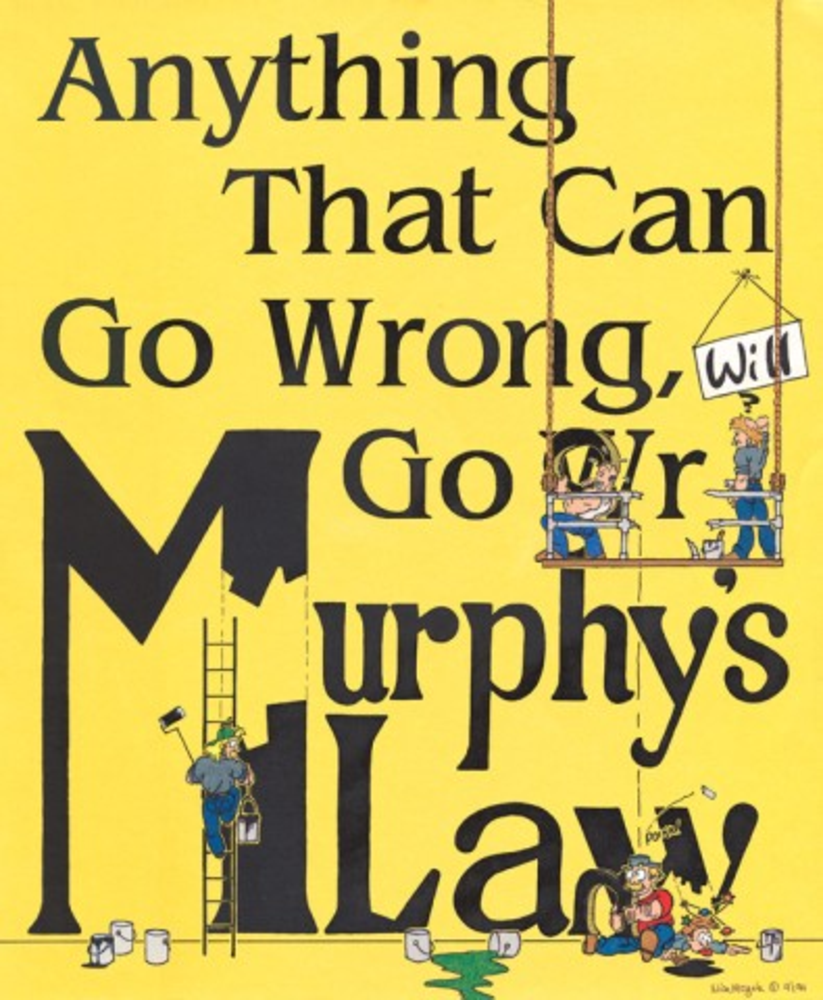
\includegraphics[height=8cm]{Section6/murphys_law}
%
%\end{center}
%
%%\end{frame}
%
%%}
%
%
%\subsection{Type I Error}
%
%%\frame{ \frametitle{Type I error}%\pause
%
%%\vspace{-2 cm}
%
%\begin{itemize}
%  \item A \textbf{Type I error} is when one rejects $H_0$ when in fact $H_0$ is true.
%  \item The probability of making a Type I error is called the \textbf{size} or \textbf{significance level} of the test and is
%  denoted by $\alpha$.
%   \item<3-> It is also known as a \textbf{false positive}.
%\end{itemize}
%
%\iffalse
%\PutAt<1-1>{(2cm,7cm)}{\NormalBox{\parbox[position]{8cm}{\begin{center}\Huge{\alert{TYPE I ERROR}}\end{center}}}}
%\PutAt<2-2>{(2cm,7cm)}{\NormalBox{\parbox[position]{8cm}{\begin{center}\Huge{\alert{SIZE $\alpha$}}\end{center}}}}
%\PutAt<3-3>{(2cm,6cm)}{\NormalBox{\parbox[position]{8cm}{\begin{center}\Huge{\alert{FALSE POSITIVE}}\end{center}}}}
%
%}
%\fi
%\subsection{Type II Error}
%
%%\frame{ \frametitle{Type II error}%\pause
%
%%\vspace{-2 cm}
%
%\begin{itemize}
%  \item A \textbf{Type II error} is when one accepts $H_0$ when in fact $H_0$ is false.
%  \item The probability of making a Type II error is denoted by \textbf{$\beta$}.
%   \item It is also known as a \textbf{false negative}.
%\end{itemize}
%\iffalse
%\PutAt<1-1>{(2cm,7cm)}{\NormalBox{\parbox[position]{8cm}{\begin{center}\Huge{\alert{TYPE II ERROR}}\end{center}}}}
%\PutAt<2-2>{(2cm,7cm)}{\NormalBox{\parbox[position]{8cm}{\begin{center}\Huge{\alert{$\beta$}}\end{center}}}}
%\PutAt<3-3>{(2cm,6cm)}{\NormalBox{\parbox[position]{8cm}{\begin{center}\Huge{\alert{FALSE NEGATIVE}}\end{center}}}}
%
%}
%\fi
%\subsection{Summary Table}
%
%%\frame{ \frametitle{Summary Table}%\pause
%
%%\vspace{-2 cm}
%
%\begin{tabular}{ccc}
%\ &Truth&Truth \\ \hline
%Statistical Decision&$H_0$&$H_a$\\ \hline
%Accept $H_0$&No error&Type II error ($\beta$)\\
%Reject $H_0$&Type I error ($\alpha$)&No error \\ \hline
%\end{tabular}
%\iffalse
%\PutAt<1-1>{(2cm,7cm)}{\NormalBox{\parbox[position]{8cm}{\begin{center}\Huge{\alert{ACCEPT $H_0$}}\end{center}}}}
%\PutAt<2-2>{(2cm,7cm)}{\NormalBox{\parbox[position]{8cm}{\begin{center}\Huge{\alert{REJECT $H_0$}}\end{center}}}}
%%\PutAt<3-3>{(2cm,6cm)}{\NormalBox{\parbox[position]{8cm}{\begin{center}\Huge{\alert{FALSE NEGATIVE}}\end{center}}}}
%
%}
%\fi
%
%\subsection{Parameters for Testing}
%%\begin{frame} \frametitle{Actual Tests (Inference)}%\pause
%
%%\vspace{-2 cm}
%\begin{itemize}
%
%\item Population mean $\mu$ which come from quantitative data.
%
%\item Population proportion $p$ which come from qualitative data.
%
%\end{itemize}
%
%\iffalse
%\PutAt<1-1>{(2cm,6cm)}{\NormalBox{\parbox[position]{8cm}{\begin{center}\Huge{\alert{QUANTITATIVE DATA}}\end{center}}}}
%\PutAt<2-2>{(2cm,6cm)}{\NormalBox{\parbox[position]{8cm}{\begin{center}\Huge{\alert{QUALITATIVE DATA}}\end{center}}}}
%
%\end{frame}
%%________________________________________________________________________
%\fi
%\subsection{Interpretation}
%
%%\frame{ \frametitle{Test Statistic Falls in Rejection Region}%\pause
%
%%\vspace{-2 cm}
%
%\begin{itemize}
%  \item we reject the null hypothesis;
%  \item conclude that the alternative is true;
%  \item and quantify that we are making this conclusion with the possibility of
%  making a 100$\alpha$\% probability of error (Type I error).
%\end{itemize}
%\iffalse
%\PutAt<1-1>{(2cm,6cm)}{\NormalBox{\parbox[position]{8cm}{\begin{center}\Huge{\alert{REJECT $H_0$}}\end{center}}}}
%\PutAt<2-2>{(2cm,6cm)}{\NormalBox{\parbox[position]{8cm}{\begin{center}\Huge{\alert{ACCEPT $H_a$}}\end{center}}}}
%\PutAt<3-3>{(2cm,6cm)}{\NormalBox{\parbox[position]{8cm}{\begin{center}\Huge{\alert{100$\alpha$\% ERROR}}\end{center}}}}
%
%}
%\fi
%%________________________________________________________________________
%
%%\subsection{Interpretation}
%
%%\frame{ \frametitle{Test Statistic Does Not Fall in Rejection Region}%\pause
%
%%\vspace{-2 cm}
%
%\begin{itemize}
%  \item we do not reject the null hypothesis;
%  \item we do not conclude that the null hypothesis is true;
%  \item because in general we do not know the probability $\beta$ of incorrectly accepting $H_0$ (Type II error).
%\end{itemize}
%
%
%\iffalse
\documentclass[12pt]{article}
\usepackage{amsmath}
\usepackage{latexsym}

\addtolength{\textwidth}{1in} \addtolength{\oddsidemargin}{-0.5in}
\addtolength{\textheight}{1.6in} \addtolength{\topmargin}{-0.8in}

\newfont{\tebbb}{msbm10 scaled\magstep1}

\newtheorem{theorem}{Theorem}[section]
\newtheorem{proposition}[theorem]{Proposition}
\newtheorem{lemma}[theorem]{Lemma}
\newtheorem{corollary}[theorem]{Corollary}
\newtheorem{remark}[theorem]{Remark}
\newtheorem{example}[theorem]{Example}
\newcommand{\beq}{\begin{equation}}
\newcommand{\eeq}{\end{equation}}
\newtheorem{definition}[theorem]{Definition}


\newcommand{\cross}[2]{{{\bf{#1}} \times {\bf{#2}}}}
\newcommand{\dotprod}[2]{{{\bf{#1}} \cdot {\bf{#2}}}}
\newcommand{\real}[1]{{\mbox{\tebbb R}}^{#1}}
\newcommand{\norm}[1]{\|{\bf{#1}}\|}
\renewcommand{\theequation}{\thesection.\arabic{equation}}

\baselineskip = 20pt plus 3pt minus 3pt

\begin{document}
\fi
\section{Suggested Exercises}\label{ssec.se3}\markright{\ref{ssec.se3} \titleref{ssec.se3}}
\begin{enumerate}
\item Which hypothesis,the null or the alternative,is the statusquo hypothesis?Which is the research hypothesis?
\item What is a test statistics?
\item Define $\alpha$ and  $\beta$. How do they relate to Type I and Type II errors?
\item If you test a hypothesis and reject the null hypothesis in favor of the alternative hypothesis,does your test prove that the alternative hypothesis is correct?Explain.
\item List all possible results of the combinations of decisions and true states of nature ofr a test of hypothesis.
\end{enumerate}

\iffalse
\begin{enumerate}
\item  Let $A=\left[
\begin{array}{rr}
2 & 3 \\ 3 & 5 \end{array} \right ]$ and calculate:
\begin{enumerate}
\item $A^{-1}$
\item (i) $4A$ \quad (ii) $(4A)^{-1}$
\item (i) $A^t$ \quad (ii) $(A^t)^{-1}$
\item (i) $A^3$ \quad (ii) $A^{-3}.$
\end{enumerate}
\item Let $B= \left[
{\begin{array}{rr}
2 & 5 \\
1 & 3
\end{array}}
 \right]$ and $A$ as above. Find
\begin{enumerate}
\item $B^{-1}$
\item (i) $AB$ \quad (ii) $(AB)^{-1}$ \quad (iii) $B^{-1}A^{-1}$
\end{enumerate}
\item For each of the following calculate the inverse.
\begin{enumerate}
\item $\left[ {\begin{array}{rrr} 1 & 0 & 2 \\ 2 & -1 & 3 \\ 4 & 1 &
8
\end{array}}
 \right]$
\item $\left[ {\begin{array}{rrr} 1 & 2 & 1 \\ 1 & 1 & 1 \\ 3 & -1 &
1
\end{array}}
 \right]$
\item $ \left[ {\begin{array}{rrr} 1 & 3 & -4 \\ 1 & 5 & -1 \\ 3 &
13 & -6
\end{array}}
 \right]
$
\item $\left[ {\begin{array}{rrr} 0 & 1 & 1 \\ 5 & 1 & -1 \\ 2 & -3
& -3
\end{array}}
 \right]$
\item $\left [\begin {array}{rrrr} 1&0&0&0\\2&-2&0&0
\\3&1&-2&0\\1&-1&3&0\end {array}
\right ]$
\item $ \left[ {\begin{array}{rrrr} 1 & 2 & 1 & 0 \\ 0 &
1 & -1 & 0 \\ 1 & 3 & 1 & -2 \\ 1 & 4 & -2 & 4
\end{array}}
\right]$
\end{enumerate}
\item Solve the following system using matrix inversion.
\begin{eqnarray*} x_1+2x_2+x_3&=&1\\
x_2-x_3&=&-1\\ x_1+3x_2+x_3-2x_4&=&-2\\ x_1+4x_2-2x_3+4x_4&=&4
\end{eqnarray*}
\item Let $A= \left[
\begin{array}{rr}
1 & 5 \\
0 & 1
\end{array}
 \right]$, $B= \left[
\begin{array}{rr}
2 & 3 \\
1 & -2
\end{array}
 \right]$ $C= \left[
\begin{array}{rr}
3 & -5 \\
-1 & 2
\end{array}
 \right]$
 $D= \left[
\begin{array}{rr}
-3 & -5 \\
7 & 2
\end{array}
 \right]$  find
\begin{enumerate}
 \item (i) $\det(A)$ \quad (ii) $\det(B)$ \quad (iii) $\det(C)$ \quad (iv) $\det(D)$
 \item (i) $\det(A+B)$ \quad (ii) $\det(A)+\det(B)$
 \item (i) $\det(3A)$ \quad (ii) $\det(B^t)$
 \item (i) $AB$ \quad (ii) $\det(AB)$ \quad (iii) $\det(A)\det(B)$
 \item $\det(D^{-1})$
\end{enumerate}
\item Let $G=\left[
{\begin{array}{rrr}
1 & 0 & 1 \\
2 & 3 & 1 \\
-7 & 0 & -7
\end{array}}
 \right]$,
$H =  \left[
{\begin{array}{rrr}
1 & 2 & 3 \\
4 & 6 & 5 \\
3 & 2 & 7
\end{array}}
 \right]$,
$J =  \left[
{\begin{array}{rrr}
-2 & 4 & -6 \\
3 & -5 & 7 \\
9 & -6 & -3
\end{array}}
 \right]$ find
\begin{enumerate}
\item (i) $\det(G)$ \quad (ii) $\det(G^t)$ \quad
\item $\det(H)$
\item $\det(J)$
\item (i) $\det(HJ)$ (ii) $\det(GJ)$
\end{enumerate}
\item Find $\det(A)$ and $\det(A^{-1})$ for
\begin{align*}
\mathrm{(a)}\ \ A &= \left[ \begin{array}{rrrr} 1 & 2 & 1 & 0 \\ 0 & 1 & -1 & 0
\\ 1 & 3 & 1 & -2 \\ 1 & 4 & -2 & 4 \end{array} \right]&
\mathrm{(b)}\ \ A&= \left[ {\begin{array}{rrrr} 10 & -3 & -3 & -2 \\ 10 & -3 &
-4 & -3 \\ -6 & 2 & 2 & 1 \\ -3 & 1 & 1 & 1 \end{array}} \right]
\end{align*}

\item We have seen that systems of equations can be solved  using either
Gaussian elimination or with ${\bf x}=A^{-1}{\bf b}$. Determine
which of the two methods are appropriate for the following two
systems.
\begin{align*}
\mathrm{(a)}\qquad \quad \quad \ x_1-x_3&=-1& \mathrm{(b)}\ \ 2x_1+x_2-x_3&=6\\
11x_1+2x_2+x_3&=2& 3x_1-x_2&=1\\
3x_1+x_2+3x_3&=1& 9x_2+2x_3&=0
\end{align*}

\end{enumerate}

\section{Answers to activity questions and suggested exercises}
\label{answers3}\markright{\ref{answers3}
\titleref{answers3}}

{\bf Activity questions}

\bigskip

\noindent {\bf \ref{ssec.definv}:}
\begin{enumerate}
\item (a), but not (b).
\item $I$.
\end{enumerate}

\bigskip

\noindent {\bf \ref{ssec.findinv}:}

\begin{enumerate}
\item \begin{enumerate}
\item
\begin{eqnarray*}
& &
\left[ \begin{array}{rrrcrrr} 1 & 0 & 1 & \vline & 1 & 0 & 0\\
                             -1 & 1 & 2 & \vline & 0 & 1 & 0\\
                              2 & 2 & 9 & \vline & 0 & 0 & 1
\end{array} \right]
\\&&\hspace{-12mm}
\overset{\begin{smallmatrix}R_2+R_1\\R_3-2R_1\end{smallmatrix}}{\leadsto}
\left[ \begin{array}{rrrcrrr} 1 & 0 & 1 & \vline & 1 & 0 & 0\\
                              0 & 1 & 3 & \vline & 1 & 1 & 0\\
                              0 & 2 & 7 & \vline & -2 & 0 & 1
\end{array} \right]
\\&&\hspace{-11mm}
\overset{R_3-2R_2}{\leadsto}
\left[ \begin{array}{rrrcrrr} 1 & 0 & 1 & \vline & 1 & 0 & 0\\
                               0 & 1 & 3 & \vline & 1 & 1 & 0\\
                               0 & 0 & 1 & \vline & -4 & -2 & 1
\end{array} \right]
\\&&\hspace{-12mm}
\overset{\begin{smallmatrix}R_1-R_3\\R_2-3R_3\end{smallmatrix}}{\leadsto}
\left[\begin{array}{rrrcrrr} 1 & 0 & 0 & \vline & 5 & 2 & -1\\
                               0 & 1 & 0 & \vline & 13 & 7 & -3\\
                               0 & 0 & 1 & \vline & -4 & -2 & 1
\end{array} \right].
\end{eqnarray*}
The inverse is
$\left[ \begin{array}{rrr} 5&2&-1\\13&7&-3\\-4&-2&1 \end{array} \right]$.
\item
\begin{eqnarray*}&&
\left[ \begin{array}{rrrcrrr} 1 & 0 & 1 & \vline & 1 & 0 & 0\\
                               1 & 1 & 0 & \vline & 0 & 1 & 0\\
                               -1 & 1 & -2 & \vline & 0 & 0 & 1
\end{array} \right]\\
 \overset{\begin{smallmatrix}R_2-R_1\\R_3+R_1\end{smallmatrix}}{\leadsto}
&&\vspace{-10mm}\left[ \begin{array}{rrrcrrr} 1 & 0 & 1 & \vline & 1 & 0 & 0\\
                              0 & 1 & -1 & \vline & -1 & 1 & 0\\
                              0 & 1 & -1 & \vline & -1 & 0 & 1
\end{array} \right]\\ \\
\overset{R_3-R_2}{\leadsto}
&&\vspace{-10mm}\left[ \begin{array}{rrrcrrr} 1 & 0 & 1 & \vline & 1 & 0 & 0\\
                               0 & 1 & -1 & \vline & -1 & 1 & 0\\
                               0 & 0 & 0 & \vline & 0 & -1 & 1
\end{array} \right].
\end{eqnarray*}
The matrix does not reduce to $I$ so $\exists$ no inverse.
\item
\begin{eqnarray*}
&&
\left[ \begin{array}{rrrrcrrrr}  1 & 0 & 0 & 0 & \vline & 1 & 0 & 0 & 0\\
                                 0 & 0 & 0 & 1 & \vline & 0 & 1 & 0 & 0\\
                                 0 & 0 & 1 & 0 & \vline & 0 & 0 & 1 & 0\\
                                 0 & 1 & 0 & 0 & \vline & 0 & 0 & 0 & 1
\end{array} \right] \\ \\\overset{R_2\leftrightarrow R_4}{\leadsto}
&&\vspace{-10mm}\left[ \begin{array}{rrrrcrrrr}  1 & 0 & 0 & 0 & \vline & 1 & 0 & 0 & 0\\
                                 0 & 1 & 0 & 0 & \vline & 0 & 0 & 0 & 1\\
                                 0 & 0 & 1 & 0 & \vline & 0 & 0 & 1 & 0\\
                                 0 & 0 & 0 & 1 & \vline & 0 & 1 & 0 & 0
\end{array} \right].
\end{eqnarray*}
 Hence this matrix is it's own inverse.

\end{enumerate}
\end{enumerate}

\bigskip

\noindent {\bf \ref{ssec.propinv}:}\\
\vspace{0.1\baselineskip}

\noindent {\bf Hints: } To prove number 5, what does
$(A^{-1})(A^{-1})^{-1}$ equal?  To prove number 7, use the exact
same method shown in the notes, except that you now multiply
$(kA)(\frac{1}{k}A^{-1}$).

\bigskip

\noindent {\bf \ref{ssec.syseinv}:}
\begin{enumerate}
\item $A^{-1}=\left [ \begin{array}{rrr}\vspace{1mm}
                                1&0&1\\ \vspace{1mm}
                                1&1&\frac{5}{2}\\
                                0&0&-\frac{1}{2} \end{array} \right
                                ]$,\  $x_1=\left [ \begin{array}{r}\vspace{1mm}
                                -2\\ \vspace{1mm}-\frac{5}{2}\\ \frac{3}{2}
                                \end{array} \right ]$,\ $x_2=\left [ \begin{array}{r} \vspace{1mm}
                                -11\\ \vspace{1mm} -\frac{13}{2}\\ \frac{1}{2}
                                \end{array} \right ]$.
\item Same as 1.

\item ${\bf x}={\bf 0}$.

\item If any other {\bf b} are introduced into the problem, by
theorem \ref{eq2invert} we know that the system will be consistent
and have exactly one solution for every {\bf b}.
\end{enumerate}

\noindent {\bf \ref{sec.det}:}
\begin{enumerate}
\item \begin{itemize} \item[(i)]
\begin{itemize}
\item[(a)] $2\left| \begin{array}{rr}2&-2\\0&1\end{array} \right| +
\left| \begin{array}{rr}3&-2\\0&1\end{array} \right| +
3 \left| \begin{array}{rr}3&2\\0&0\end{array} \right| = 4+3+0 = 7$
\item[(b)] $1\left| \begin{array}{rr}3&-2\\0&1\end{array} \right| +
2\left| \begin{array}{rr}2&3\\0&1\end{array} \right| +
0\left| \begin{array}{rr}2&3\\3&-2\end{array} \right| = 3+4+0 = 7$
\end{itemize}
\item[(ii)]
\begin{itemize}
\item[(a)] $2\left| \begin{array}{rr}1&2\\8&3\end{array} \right| -
3\left| \begin{array}{rr}0&2\\0&3\end{array} \right| +
2\left| \begin{array}{rr}0&1\\0&8\end{array} \right| = -26+0+0 = -26$
% START HERE
\item[(b)] $-3\left| \begin{array}{rr}0&2\\0&3\end{array} \right| +
1\left| \begin{array}{rr}2&2\\0&3\end{array} \right| -
8\left| \begin{array}{rr}2&2\\0&2\end{array} \right| = 0+6-32 = -26$
\end{itemize}
\end{itemize}
\item Expand matrix (i) along the bottom row
$$
\left| \begin{array}{rr}2&-1\\3&2\end{array}\right|
$$
Expand matrix (ii) along the bottom row
$$
2 \left| \begin{array}{rr}1&2\\8&3\end{array} \right| = 2(3-16) = -26
$$
\end{enumerate}

\noindent {\bf \ref{ssec.propdet}:}
\begin{enumerate}
\item
\begin{enumerate}
\item
$$
\begin{vmatrix}2&2&1\\2&1&1\\1&2&1\end{vmatrix} \overset{R_1 - R_3}{\leadsto}
\begin{vmatrix}1&0&0\\2&1&1\\1&2&1\end{vmatrix} = \begin{vmatrix}1&1\\2&1\end{vmatrix} = 1-2 =-1
$$
\item
\begin{eqnarray*}
\left| \begin{array}{rrrr} 1&2&7&5\\2&1&3&10\\4&-1&-3&20\\8&3&9&39
\end{array} \right|
&& \hspace{-5mm}\overset{\begin{smallmatrix}C_4 -
5C_1\\C_3-3C_2\end{smallmatrix}}{\leadsto} \quad \left|
\begin{array}{rrrr} 1&2&1&0\\2&1&0&0\\4&-1&0&0\\8&3&0&-1
\end{array} \right|\\
&=&
- \left| \begin{array}{rrr} 1&2&1\\2&1&0\\4&-1&0\end{array} \right| \\
&=& - \left| \begin{array}{rr}2&1\\4&-1\end{array} \right| \\&=&
-(-2-4) = 6
\end{eqnarray*}
\end{enumerate}
\item
\begin{enumerate}
\item -3
\item 270
\item -60
\item Not enough information
\end{enumerate}
\end{enumerate}
\noindent {\bf \ref{ssec.adjoint}:}  $A$ is invertible, since
det($A$)=17;  det($A^{-1}$)$=\frac{1}{17}$.


\bigskip

\noindent {\bf Suggested Exercises}

\begin{enumerate}
\item
\begin{enumerate}\item$ \left[ {\begin{array}{rr}5&-3\\-3&2 \end{array}}
\right]$\\
\item(i) $\left[ {\begin{array}{rr}8&12\\12&20\end{array}}
 \right]$\quad
(ii) $\left[ {\begin{array}{rr} \frac {5}{4}  & -\frac {3}{4}\\ -\frac {3}{4}  & \frac {1}{2}
\end{array}} \right]$
\item (i) $\left[ {\begin{array}{rr} 2 & 3 \\ 3 & 5 \end{array}}
\right]$ \quad (ii) $\left[ {\begin{array}{rr} 5 & -3 \\ -3 &
2\end{array}} \right]$
\item (i) $\left[ {\begin{array}{rr} 89 &
144
\\ 144 & 233
\end{array}}
 \right]$\quad
(ii) $
 \left[
{\begin{array}{rr}
233 & -144 \\
-144 & 89
\end{array}}
 \right]$
 \end{enumerate}

\item \begin{enumerate}
\item $ \left[
\begin{array}{rr}
3 & -5 \\
-1 & 2
\end{array}
 \right]$\\
\item (i) $\left[ {\begin{array}{rr} 7 & 19 \\ 11 & 30
\end{array}}
 \right]$ \quad (ii) $ \left[
{\begin{array}{rr}
30 & -19 \\
-11 & 7
\end{array}}
 \right]$ \quad (iii) $ \left[ {\begin{array}{rr} 30 & -19 \\ -11 & 7
\end{array}}
 \right]$
 \end{enumerate}
\item \begin{enumerate}
\item $ \left[ {\begin{array}{rrr} -11 & 2 & 2 \\ -4 & 0 & 1 \\ 6 &
-1 & -1
\end{array}}
 \right]
$
\item $\left[ {\begin{array}{rrr}\vspace{1mm} 1 & -\frac {3}{2}& \frac {1}{2}\\ \vspace{1mm}
1 & -1 & 0 \\ -2 & \frac {7}{2}  & -\frac {1}{2}
\end{array}}
 \right]$
\item Not Possible Singular matrix
\item $\left[ {\begin{array}{rrr}\vspace{1mm} \frac {3}{2} & 0 & \frac
{1}{2}\\ \vspace{1mm} -\frac {13}{4}  & \frac {1}{2} & -\frac {5}{4}  \\ \frac
{17}{4} & -\frac {1}{2} & \frac {5}{4}
\end{array}}
 \right]$
\item Not Possible \item $\left[ {\begin{array}{rccc} 10 & 10 & -6 &
-3
\\ -3 & -3 & 2 & 1 \\  -3 & -4  &
2& 1 \\-1 & -\frac{3}{2} & \frac{1}{2} & \frac{1}{2}
\end{array}}
\right]$
\end{enumerate}
\item $x_1=0,\ x_2=0,\ x_3=1,\ x_4=\tfrac{3}{2}$
\item
\begin{enumerate}
\item (i) 1 (ii) -7 (iii) 1 (iv) 29
\item (i) -11 (ii) -6
\item (i) 9 (ii) -7
\item (i) $ \begin{vmatrix} 7 & -7 \\1 & -2 \end{vmatrix}$ (ii) -7 (iii) -7
\item $\tfrac{1}{29}$
\end{enumerate}
\item
\begin{enumerate}
\item (i) 0 (ii) 0
\item -24
\item 12
\end{enumerate}
\item
\begin{enumerate}
\item (i) 2 (ii) $\frac{1}{2}$
\item (i) 1 (ii) 1
\end{enumerate}
\item
\begin{enumerate}
\item The determinant of the system is $0$, therefore $A$ is not
invertible and the system must be solved using Gaussian
elimination.
\item The determinant is not 0; either method works.
\end{enumerate}
\end{enumerate}

%\end{document}
\fi

%\iffalse
%\PutAt<1-1>{(2cm,6cm)}{\NormalBox{\parbox[position]{8cm}{\begin{center}\Huge{\alert{DO NOT REJECT $H_0$}}\end{center}}}}
%\PutAt<2-2>{(2cm,6cm)}{\NormalBox{\parbox[position]{8cm}{\begin{center}\Huge{\alert{RESERVE JUDGEMENT ON $H_0$}}\end{center}}}}
%\PutAt<3-3>{(2cm,6cm)}{\NormalBox{\parbox[position]{8cm}{\begin{center}\Huge{\alert{DO NOT KNOW $\beta$}}\end{center}}}}
%
%}
%
%\subsection{Exercises}
%
%\begin{frame} \frametitle{Exercises}%\pause
%
%\noindent 11th edition, p. 329:  6.1--6.7.
%
%\bigskip
%
%\noindent 10th edition, p. 350:  6.1--6.7.
%
%\end{frame}
%
%%________________________________________________________________________
%\fi
%
%\section{Large Sample Test for a Single Mean}
%
%\subsection{Large Sample Test for a Single Mean}
%
%%\frame{ \frametitle{Hypothesis Test for a Single Mean}%\pause
%
%%\vspace{-1.5 cm}
%
%For a given population mean $\mu$ we want to formulate a null hypothesis with respect to
%some fixed level, thus
%\[H_0:  \ \mu = \mu_0.\]
%Then we can have,
%
%\begin{itemize}
%  \item A \textbf{one tailed, upper test} where $H_a$ says $\mu > \mu_0$.
%  \item A \textbf{one tailed, lower test} where $H_a$ says $\mu < \mu_0$.
%  \item A \textbf{two tailed test} where $H_a$ says $\mu \neq \mu_0$.
%\end{itemize}
%\iffalse
%\PutAt<1-1>{(2cm,7cm)}{\NormalBox{\parbox[position]{8cm}{\begin{center}\Huge{\alert{$\mu > \mu_0$}}\end{center}}}}
%\PutAt<2-2>{(2cm,7cm)}{\NormalBox{\parbox[position]{8cm}{\begin{center}\Huge{\alert{$\mu > \mu_0$}}\end{center}}}}
%\PutAt<3-3>{(2cm,7cm)}{\NormalBox{\parbox[position]{8cm}{\begin{center}\Huge{\alert{$\mu \neq \mu_0$}}\end{center}}}}
%
%}
%\fi
%\subsection{Test Statistic}
%
%%\frame{ \frametitle{Test Statistic}%\pause
%
%%\vspace{-2 cm}
%
%Let $x_1,\ldots , x_n$ be a random sample from a population that has unknown mean $\mu$
%and standard deviation $\sigma$.  Compute,
%\begin{itemize}
%  \item the sample mean
%  \item the sample standard deviation
%  \item test statistic
%\end{itemize}
%\iffalse
%\PutAt<1-1>{(2cm,6cm)}{\NormalBox{\parbox[position]{8cm}{\begin{center}\Huge{$\bar{x}=\frac1n \sum x_i$}\end{center}}}}
%\PutAt<2-2>{(1cm,6cm)}{\NormalBox{\parbox[position]{10cm}{\begin{center}\Huge{$s=\sqrt{\frac{1}{n-1}\sum \left(x_i -\bar{x}\right)^2}$}\end{center}}}}
%\PutAt<3-3>{(2cm,6cm)}{\NormalBox{\parbox[position]{8cm}{\begin{center}\Huge{$z= \frac{\bar{x}-\mu_0}{s/\sqrt{n}}$}\end{center}}}}
%
%
%}
%\fi
%\subsection{Rejection Region}
%
%%\frame{ \frametitle{Rejection Region - One Tailed Test}%\pause
%
%%\vspace{-2 cm}
%
%Fix $\alpha > 0$ (usually $\alpha = 0.05$) so that
%\[P\left(z > z_\alpha \right) = P\left(z <  -z_\alpha \right) = \alpha \]
%where $z$ denotes a standard normal random variable:
%\begin{itemize}
%  \item one tailed upper test, reject $H_0:  \ \mu = \mu_0$ if
%  \item one tailed lower test, reject $H_0:  \ \mu = \mu_0$ if
%\end{itemize}
%\iffalse
%\PutAt<1-1>{(2cm,6cm)}{\NormalBox{\parbox[position]{8cm}{\begin{center}\Huge{$z= \frac{\bar{x}-\mu_0}{s/\sqrt{n}} > z_\alpha$}\end{center}}}}
%\PutAt<2-2>{(2cm,6cm)}{\NormalBox{\parbox[position]{10cm}{\begin{center}\Huge{$z= \frac{\bar{x}-\mu_0}{s/\sqrt{n}} < -z_\alpha$}\end{center}}}}
%
%
%
%}
%\fi
%\subsection{Rejection Region}
%
%%\frame{ \frametitle{Rejection Region - Two Tailed Test}%\pause
%
%%\vspace{-2 cm}
%
%Fix $\alpha > 0$ (usually $\alpha = 0.05$) so that
%\[P\left(z > z_{\alpha/2} \right) = P\left(z <  -z_{\alpha/2} \right) = {\alpha/2} \]
%where $z$ denotes a standard normal random variable:
%\begin{itemize}
%%  \item<1-> two tailed test, reject $H_0:  \ \mu = \mu_0$ if
%  \item two tailed test, reject $H_0:  \ \mu = \mu_0$ if
%\end{itemize}
%
%%\PutAt<1-1>{(2cm,6cm)}{\NormalBox{\parbox[position]{8cm}{\begin{center}\Huge{$z= \frac{\bar{x}-\mu_0}{s/\sqrt{n}} > z_\alpha/2$}\end{center}}}}
%%\PutAt<2-2>{(2cm,6cm)}{\NormalBox{\parbox[position]{10cm}{\begin{center}\Huge{$z= \frac{\bar{x}-\mu_0}{s/\sqrt{n}} < -z_\alpha/2$}\end{center}}}}
%%\PutAt<2-2>{(2cm,6cm)}{\NormalBox{\parbox[position]{10cm}{\begin{center}\Huge{$|z|= \left|\frac{\bar{x}-\mu_0}{s/\sqrt{n}}\right| > z_{ \alpha/2}$}\end{center}}}}
%
%
%
%%}
%
%\subsection{Interpretation}
%
%%\frame{ \frametitle{Test Statistic Falls in Rejection Region}%\pause
%
%%\vspace{-2 cm}
%
%\begin{itemize}
%  \item we reject the null hypothesis;
%  \item conclude that the alternative is true;
%  \item and quantify that we are making this conclusion with the possibility of
%  making a 100$\alpha$\% probability of error (Type I error).
%\end{itemize}
%\iffalse
%\PutAt<1-1>{(2cm,6cm)}{\NormalBox{\parbox[position]{8cm}{\begin{center}\Huge{\alert{REJECT $H_0$}}\end{center}}}}
%\PutAt<2-2>{(2cm,6cm)}{\NormalBox{\parbox[position]{8cm}{\begin{center}\Huge{\alert{ACCEPT $H_a$}}\end{center}}}}
%\PutAt<3-3>{(2cm,6cm)}{\NormalBox{\parbox[position]{8cm}{\begin{center}\Huge{\alert{100$\alpha$\% ERROR}}\end{center}}}}
%
%}
%%________________________________________________________________________
%
%%\subsection{Interpretation}
%
%\frame{ \frametitle{Test Statistic Does Not Fall in Rejection Region}%\pause
%
%\vspace{-2 cm}
%\fi
%\begin{itemize}
%  \item we do not reject the null hypothesis;
%  \item we do not conclude that the null hypothesis is true;
%  \item because in general we do not know the probability $\beta$ of incorrectly accepting $H_0$ (Type II error).
%\end{itemize}
%\iffalse
%\PutAt<1-1>{(2cm,6cm)}{\NormalBox{\parbox[position]{8cm}{\begin{center}\Huge{\alert{DO NOT REJECT $H_0$}}\end{center}}}}
%\PutAt<2-2>{(2cm,6cm)}{\NormalBox{\parbox[position]{8cm}{\begin{center}\Huge{\alert{RESERVE JUDGEMENT ON $H_0$}}\end{center}}}}
%\PutAt<3-3>{(2cm,6cm)}{\NormalBox{\parbox[position]{8cm}{\begin{center}\Huge{\alert{DO NOT KNOW $\beta$}}\end{center}}}}
%
%}
%\fi
%\subsection{Examples}
%
%%\begin{frame} \frametitle{Examples}%\pause
%
%Will be discussed in class.
%
%%\end{frame}
%




\subsection{Exercises}
\begin{enumerate}
\item Suppose $P(A)=0.5$,$P(B)=0.8$,and $P(A\bigcap B)=0.4$.Find the following probabilities:
\begin{enumerate}
\item Find $P(A^{c})$ 
\item Find $P(A\bigcup B)$
\item Find $P(A\bigcap B^{c})$
\end{enumerate}

\item An experiment is conducted in which the outcomes of each of the two variables are observed.The two variables are Gender \{Male,Female\} and Age\{$\leq 30$,30-50,$\geq50$\}.The probabilities associated with each of the six possible outcome pairs are given as follows:
\begin{center}
\begin{tabular}{|c|c|c|c|}\hline
             &$\leq 30$&30-50&$\geq50$\\ \hline   
Male         &0.50     &0.10 &0.05\\ \hline
Female       &0.25     &0.07 &0.03\\ \hline
\end{tabular}
\end{center}
\begin{enumerate}
\item Find $P$(\{Male\})
\item Find $P$(\{Female or 30-50\})
\item Find $P$(\{$\leq$ 30\})
\item Find $P$(\{$\leq$ 30 and Female\})
\end{enumerate}


\item A pair of fair dice is tossed.Considering the following events:\\
%\begin{description}
$A$: \{The sum of the dots on the up faces of the two dice is 8\}.\\
$B$: \{at least one of the two dice showing is 3\}.

% \end{description}

\begin{enumerate}
\item Identify the sample points in the events $A,B,A\bigcap B,A\bigcup B$,and $A^{c}$.
\item Find the corresponding probabilities in part (a). 
\item Apply additive rule to $P$($A \bigcup B$).
\item Are the events $A$ and $B$ mutually exclusive?Why?
\end{enumerate}



\iffalse
\item Two balls are drawn at random and without replacement from a box containing two blue balls and two red balls.
\begin{enumerate}
\item List the sample points for this experiment.
\item Assign probabilities to the sample points.
\item Find the probability of the following events:
\begin{enumerate}
\item \{two red balls are drawn\}
\item \{One red and one blue are drawn\}
\item \{two balls with the same color are drawn\}
\end{enumerate}
\item The diagram below describes the sample space of a particular experiment and events A and B.
\begin{enumerate}
\item What is the name of the diagram?
\item Assume the sample points have the same probability.Find P(A),P(B) and P(C) .

\end{enumerate}
\end{enumerate}
\fi
%\item Show that if two $n \times n$ matrices $L$, $M$ are symmetric, then so are $L+M$ and $kL$.

\end{enumerate}
%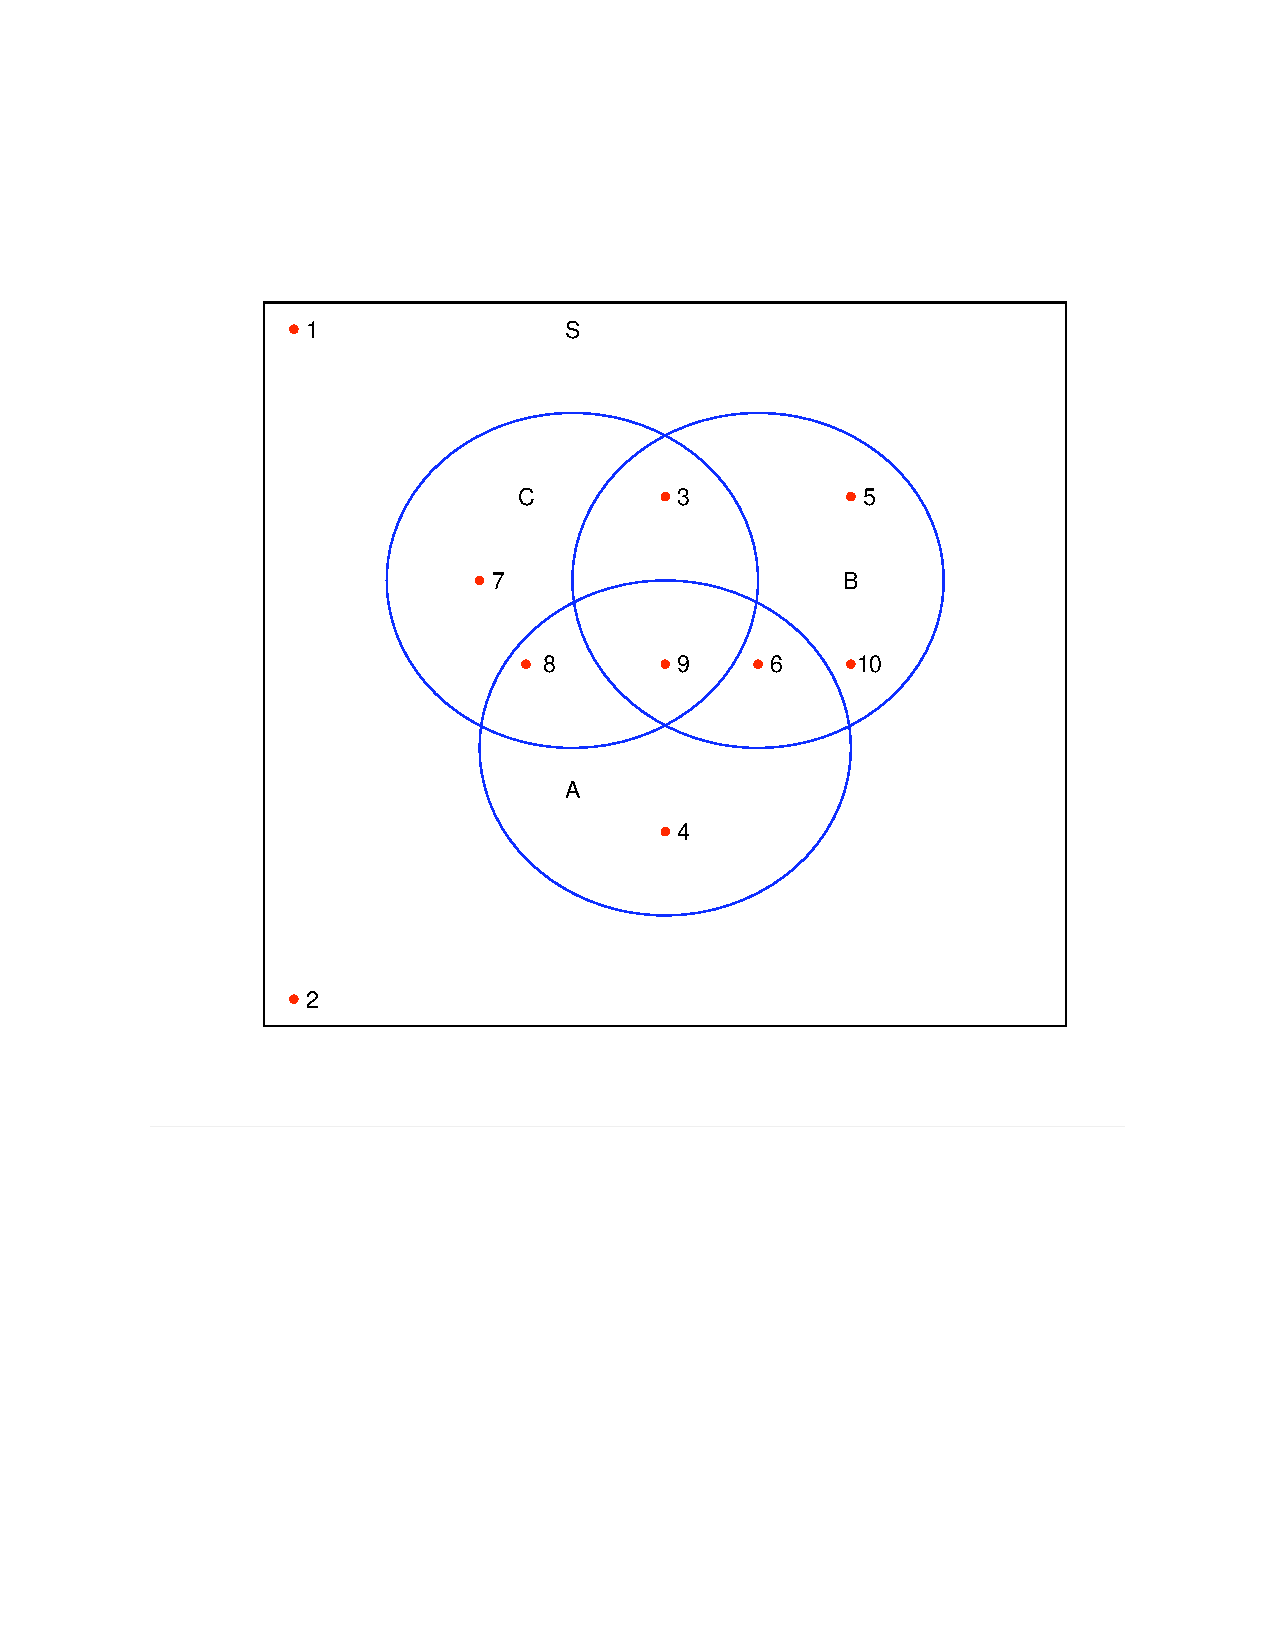
\includegraphics[height=12cm]{a2-fig-2}
\iffalse
\label{se1} \markright{\ref{se1}
\titleref{se1}}
For the following exercises, let\\ $A=[1\ 2],\ B=\left[
\begin{array}{c}3\\2 \end{array}\right ],\ C=\left [\begin
{array}{rr} 1&-2\\2&-3\end {array} \right ],\ D=\left [\begin
{array}{rr} -2&-5\\1&3\end {array} \right ],\\ E=\left [\begin
{array}{rr} 1&5\\3&8
\\2&1\end {array}\right ],\
F=\left [\begin {array}{rrr} 2&-4&1\\6&-9&1\\4&1&6\\1&7&-5\end {array}\right],\
G=\left [\begin {array}{rrr} 1&2&6\\2&-3&7
\\4&-1&3\end {array}\right ],\\
H=\left [\begin {array}{rrr} 1&0&0\\0&1&0
\\-1&0&0\end {array}\right ],\
I=\left [\begin {array}{rrr} 1&0&0\\0&1&0
\\0&0&1\end {array}\right ],\
K=\left [\begin {array}{rrrr} 1&-2&4&7\\2&3&5&-4
\\1&4&2&1\\-2&1&9&4\end {array}
\right ].$
\bigskip

\begin{enumerate}
\item Which of the following operations are not defined? If they
are defined, what is the size of the resulting matrix
\begin{enumerate}
\item $AC$
\item $CA$
\item $KF^t$
\item $KF$
\item $EB+A^t$
\item $E(H+I)$
\end{enumerate}
\item Find: a) $C+D$\quad b) $D+C$ \quad  c) $G+H$ \quad
d) $D-3C$ \quad e) $2D$
\item Find:
\begin{enumerate} \item $AB$ and $BA$
\item $(C+2D)+BA$ and $C+(2D+BA)$
\item $DC$, $ED$, $(ED)C$ and $E(DC)$
\item $FH+FG$ and $F(G+H)$
\item $G^t$, $H^t$, $(GH)^t$, $G^tH^t$ and $H^tG^t$.
\end{enumerate}
\item Find: $KF$, $FG$ and $FH$.
\item Find tr($K$), tr($I$) and tr($E$).
\item Find $C^3$ and $H^2$.
\item Find $I-H$  and $(I-H)^2$.
\item If $f(x)=x^{2} +2x+2$, $g(x)=x^{2}-x-1$, find
\begin{enumerate} \item $f(C), {\rm (b)}~f(D), {\rm (c)}~g(C), {\rm (d)}~g(D)$.
\end{enumerate}
\item Show that if two $n \times n$ matrices $L$, $M$ are symmetric, then so are $L+M$ and $kL$.

\end{enumerate}



\iffalse
\section{Maple Exercises (optional)}

As in the previous session, first open the linear algebra package.

\begin{maplegroup}
\begin{mapleinput}
\mapleinline{active}{1d}{with(linalg):}{%
}
\end{mapleinput}

\end{maplegroup}
\bigskip

In this chapter, matrix operations and the matrix form of a linear
system ( $A{\bf x}={\bf b}$) were introduced.

We will begin this session by giving a second command to construct
a matrix (the first command was given during the previous Maple
session).

\bigskip

\begin{maplegroup}
\begin{mapleinput}
\mapleinline{active}{1d}{A := matrix(3,3, [1,2,3,2,3,4,3,4,5]);}{%
}
\end{mapleinput}

\mapleresult
\begin{maplelatex}
\[
A :=  \left[ {\begin{array}{rrr} 1 & 2 & 3 \\ 2 & 3 & 4 \\ 3 & 4 &
5
\end{array}}
 \right]
\]
\end{maplelatex}

\end{maplegroup}
\begin{maplegroup}
\begin{mapleinput}
\mapleinline{active}{1d}{B:=matrix(3,3,[2,5,7,13,3,5,6,7,8]);}{%
}
\end{mapleinput}

\mapleresult
\begin{maplelatex}
\[
B :=  \left[ {\begin{array}{rrr} 2 & 5 & 7 \\ 13 & 3 & 5 \\ 6 & 7
& 8
\end{array}}
 \right]
\]
\end{maplelatex}

\end{maplegroup}
\begin{maplegroup}
\begin{mapleinput}
\mapleinline{active}{1d}{C:=matrix(4,3,[1,3,5,7,9,0,8,6,4,2,1,7]);}{%
}
\end{mapleinput}

\mapleresult
\begin{maplelatex}
\[
C :=  \left[ {\begin{array}{rrr} 1 & 3 & 5 \\ 7 & 9 & 0 \\ 8 & 6 &
4 \\ 2 & 1 & 7
\end{array}}
 \right]
\]
\end{maplelatex}

\end{maplegroup}
\begin{maplegroup}
\begin{mapleinput}
\mapleinline{active}{1d}{E:=matrix(3,4,[3,4,7,6,9,2,8,2,6,8,3,12]);}{%
}
\end{mapleinput}

\mapleresult
\begin{maplelatex}
\[
E :=  \left[ {\begin{array}{rrrr} 3 & 4 & 7 & 6 \\ 9 & 2 & 8 & 2
\\ 6 & 8 & 3 & 12
\end{array}}
 \right]
\]
\end{maplelatex}

\end{maplegroup}
\bigskip

{\bf Note:} You can not let a matrix be $D$, a Maple error will
result.

Now that we have a few matrices at hand, we will perform some
matrix operations on them. First, scalar multiplication and matrix
addition. These operations are accomplished using the commands:
scalarmul(\emph{matrix name}, \emph{scalar value}) and
matadd(\emph{matrix name},\emph{matrix name}).

\bigskip

\begin{maplegroup}
\begin{mapleinput}
\mapleinline{active}{1d}{scalarmul(B,2);}{%
}
\end{mapleinput}

\mapleresult
\begin{maplelatex}
\[
 \left[
{\begin{array}{rrr} 4 & 10 & 14 \\ 26 & 6 & 10 \\ 12 & 14 & 16
\end{array}}
 \right]
\]
\end{maplelatex}

\end{maplegroup}
\begin{maplegroup}
\begin{mapleinput}
\mapleinline{active}{1d}{matadd(A , B);}{%
}
\end{mapleinput}

\mapleresult
\begin{maplelatex}
\[
 \left[
{\begin{array}{rrr} 3 & 7 & 10 \\ 15 & 6 & 9 \\ 9 & 11 & 13
\end{array}}
 \right]
\]
\end{maplelatex}

\end{maplegroup}
\bigskip

The `matadd' command can also be used to add scalar multiples of
one matrix to another matrix in the following way.
\bigskip

\begin{maplegroup}
\begin{mapleinput}
\mapleinline{active}{1d}{matadd(3*A,-B);}{%
}
\end{mapleinput}

\mapleresult
\begin{maplelatex}
\[
 \left[
{\begin{array}{rrr} 1 & 1 & 2 \\ -7 & 6 & 7 \\ 3 & 5 & 7
\end{array}}
 \right]
\]
\end{maplelatex}

\end{maplegroup}
\begin{maplegroup}
Matrix multiplication is performed using the `multiply' command.

\end{maplegroup}
\begin{maplegroup}
\begin{mapleinput}
\mapleinline{active}{1d}{multiply(A,B);}{%
}
\end{mapleinput}

\mapleresult
\begin{maplelatex}
\[
 \left[
{\begin{array}{rrr} 46 & 32 & 41 \\ 67 & 47 & 61 \\ 88 & 62 & 81
\end{array}}
 \right]
\]
\end{maplelatex}

\end{maplegroup}
\begin{maplegroup}
\begin{mapleinput}
\mapleinline{active}{1d}{multiply(A,B,E);}{%
}
\end{mapleinput}

\mapleresult
\begin{maplelatex}
\[
 \left[
{\begin{array}{rrrr} 672 & 576 & 701 & 832 \\ 990 & 850 & 1028 &
1228 \\ 1308 & 1124 & 1355 & 1624
\end{array}}
 \right]
\]
\end{maplelatex}

\end{maplegroup}
\bigskip

As shown in the previous section, Maple can be used to solve
systems of equations using the row reduction technique. A second
method uses the `linsolve' command. If we have the system $A{\bf
x}={\bf b}$, this command solves for {\bf x}. This command will be
demonstrated with the matrix $B$ from above, and a row matrix or
vector, $b$.

\bigskip

\begin{maplegroup}
\begin{mapleinput}
\mapleinline{active}{1d}{b:=vector([2,3,6]);}{%
}
\end{mapleinput}

\mapleresult
\begin{maplelatex}
\[
b := [2, \,3, \,6]
\]
\end{maplelatex}

\end{maplegroup}
\begin{maplegroup}
\begin{mapleinput}
\mapleinline{active}{1d}{linsolve(B,b);}{%
}
\end{mapleinput}

\mapleresult
\begin{maplelatex}
\[
 \left[  \! {\displaystyle \frac {29}{119}} , \,{\displaystyle
\frac {260}{119}} , \,{\displaystyle -\frac {160}{119}}  \!
 \right]
\]
\end{maplelatex}

\end{maplegroup}
\bigskip

Try solving the same system using the techniques and commands of
the previous Maple session.

The transpose of a matrix was also defined in this section. On
Maple, the transpose of a matrix is found with the `transpose'
command.
\bigskip

\begin{maplegroup}
\begin{mapleinput}
\mapleinline{active}{1d}{transpose(A);}{%
}
\end{mapleinput}

\mapleresult
\begin{maplelatex}
\[
 \left[
{\begin{array}{rrr} 1 & 2 & 3 \\ 2 & 3 & 4 \\ 3 & 4 & 5
\end{array}}
 \right]
\]
\end{maplelatex}

\end{maplegroup}
\begin{maplegroup}
\mapleresult
\begin{maplettyout}
\end{maplettyout}

\end{maplegroup}
\bigskip

Again you might want to try some other examples for yourself.  You
can also combine the commands to simplify long strings of
calculations. \fi

\section{Answers to activity questions and suggested exercises}
\label{answers2}

{\bf Activity questions}

\bigskip

\noindent {\bf \ref{ssec.arith}:} \quad 1.Yes.

\bigskip

\noindent{\bf \ref{ssec.propma}:} \quad Yes.

\bigskip


\noindent{\bf Suggested exercises}

\begin{enumerate}
\item \begin{enumerate}
\item $1 \times 2$
\item undefined
\item undefined
\item $4 \times 3$
\item undefined
\item undefined \end{enumerate}
\item a) $\left [\begin {array}{rr} -1&-7\\3&0\end {array}
\right ]$
b) $\left [\begin {array}{rr} -1&-7\\3&0\end {array}
\right ]$
c) $\left [\begin {array}{rrr} 2&2&6\\2&-2&7
\\3&-1&3\end {array}\right ]$
\\
d) $\left [\begin {array}{rr} -5&1\\-5&12\end {array} \right ]$ e)
$\left [\begin {array}{rr} -4&-10\\2&6\end {array} \right ]$
\item  \begin{enumerate} \item $7$, $\quad \left [\begin {array}{rr} 3&6\\2&4\end {array} \right ]$
\item $\left [\begin {array}{rr} 0&-6\\6&7\end {array}
\right ]$
\item  $\left [\begin {array}{rrr} -12&19\\7&-11\end {array}
\right ]$,  $\left [\begin {array}{rrr} 3&10\\2&9
\\-3&-7\end {array}\right ]$,  $\left [\begin {array}{rr} 23&-36\\20&-31
\\-17&27\end {array}\right ]$,  $\left [\begin {array}{rr} 23&-36\\20&-31
\\-17&27\end {array}\right ]$
\item $\left [\begin {array}{rrr} -1&11&-13\\-3&29&-24
\\28&0&49\\1&-7&40\end {array}
\right ]$, \quad $\left [\begin {array}{rrr} -1&11&-13\\-3&29&-24
\\28&0&49\\1&-7&40\end {array}
\right ]$
\item $G^t=\left [\begin {array}{rrr} 1&2&4\\2&-3&-1
\\6&7&3\end {array}\right ]$, \quad $H^t=\left [\begin {array}{rrr} 1&0&-1\\0&1&0
\\0&0&0\end {array}\right ]$, \\$(GH)^t=\left [\begin {array}{rrr} -5&-5&1\\2&-3&-1
\\0&0&0\end {array}\right ]$ \\

$G^tH^t=\left [\begin {array}{rrr} 1&2&-1\\2&-3&-2
\\6&7&-6\end {array}\right ]$, \quad $H^tG^t=\left [\begin {array}{rrr} -5&-5&1\\2&-3&-1
\\0&0&0\end {array}\right ]$
\end{enumerate}
\item $KF=\left [\begin {array}{rrr} 13&67&-12\\38&-58&55
\\35&-31&12\\42&36&33\end {array}
\right ]$, \quad  $FG=\left [\begin {array}{rrr}
-2&15&-13\\-8&38&-24
\\30&-1&49\\-5&-14&40\end {array}
\right ]$, \\ $FH=\left [\begin {array}{rrr} 1&-4&0\\5&-9&0
\\-2&1&0\\6&7&0\end {array}\right
]$
\item $10$, $3$, $E$ is not square
\item $C^3=\left [\begin {array}{rr} 5&-6\\6&-7\end {array}
\right ]$,\quad $H^2=\left [\begin {array}{rrr} 1&0&0\\0&1&0
\\-1&0&0\end {array}\right ]$
\item $\left [\begin {array}{rrr} 0&0&0\\0&0&0
\\1&0&1\end {array}\right ]$

\item a) $\left [\begin {array}{rr} 1&0\\0&1\end {array} \right ]$
b) $\left [\begin {array}{rr} -3&-15\\3&12\end {array} \right ]$
c) $\left [\begin {array}{rr} -5&6\\-6&7
\\\end {array}\right ]$
d) $\left [\begin {array}{rr} 0&0\\0&0\end {array} \right ]$

\item $(L+M)^{t}=L^{t}+M^{t}=L+M$, $(kL)^{t}=kL^{t}=kL$.
\end{enumerate}

%\end{document}
\fi 
%\iffalse
%\subsection{Exercises}
%
%\begin{frame} \frametitle{Exercises}%\pause
%
%\noindent 11th edition, p. 329,  6.8; p. 334, 6.19 -- 6.21.
%
%\bigskip
%
%\noindent 10th edition, p. 357,  6.17--6.20.
%
%\end{frame}
%\fi
%
%\section{Large Sample Test for a Single Proportion}
%
%\subsection{Large Sample Test for a Single Proportion}
%
%%\frame{ \frametitle{Hypothesis Test for a Single Proportion}%\pause
%
%%\vspace{-1.5 cm}
%
%For a given population proportion $p$ we want to formulate a null hypothesis with respect to
%some fixed level, thus
%\[H_0:  \ p = p_0.\]
%Then we can have,
%
%\begin{itemize}
%  \item[1.] A \textbf{one tailed, upper test} where $H_a$ says $p > p_0$.
%  \item[2.] A \textbf{one tailed, lower test} where $H_a$ says $p < p_0$.
%  \item[3.] A \textbf{two tailed test} where $H_a$ says $p \neq p_0$.
%\end{itemize}
%\iffalse
%\PutAt<1-1>{(2cm,7cm)}{\NormalBox{\parbox[position]{8cm}{\begin{center}\Huge{\alert{$p > p_0$}}\end{center}}}}
%\PutAt<2-2>{(2cm,7cm)}{\NormalBox{\parbox[position]{8cm}{\begin{center}\Huge{\alert{$p > p_0$}}\end{center}}}}
%\PutAt<3-3>{(2cm,7cm)}{\NormalBox{\parbox[position]{8cm}{\begin{center}\Huge{\alert{$p \neq p_0$}}\end{center}}}}
%
%}
%\fi
%\subsection{Test Statistic}
%
%%\frame{ \frametitle{Test Statistic}%\pause
%
%%\vspace{-2 cm}
%
%Let $x_1,\ldots , x_n$ be a random sample from a binomial population that has unknown $p$.  Compute
%\begin{itemize}
%  \item[1.] the sample proportion
%  \item[2.] the sample error, where $q_0=1-p_0$
%  \item[3.] test statistic and suppose $np_0 \geq 15$ and $nq_0 \geq 15$
%\end{itemize}
%\iffalse
%\PutAt<1-1>{(2cm,6cm)}{\NormalBox{\parbox[position]{8cm}{\begin{center}\Huge{$\hat{p}=\frac1n \sum x_i$}\end{center}}}}
%\PutAt<2-2>{(2cm,6cm)}{\NormalBox{\parbox[position]{10cm}{\begin{center}\Huge{
%$\sigma_{\hat{p}}=\sqrt{\frac{p_0q_0}{n}}$}\end{center}}}}
%\PutAt<3-3>{(2cm,6cm)}{\NormalBox{\parbox[position]{8cm}{\begin{center}\Huge{$z= \frac{\hat{p}-p_0}{\sigma_{\hat{p}}}$}\end{center}}}}
%
%
%}
%\fi
%\subsection{Rejection Region}
%
%%\frame{ \frametitle{Rejection Region - One Tailed Test}%\pause
%
%%\vspace{-2 cm}
%
%Fix $\alpha > 0$ (usually $\alpha = 0.05$) so that
%\[P\left(z > z_\alpha \right) = P\left(z <  -z_\alpha \right) = \alpha \]
%where $z$ denotes a standard normal random variable:
%\begin{itemize}
%  \item[1.] one tailed upper test, reject $H_0:  \ p = p_0$ if
%  \item[2.] one tailed lower test, reject $H_0:  \ p = p_0$ if
%\end{itemize}
%\iffalse
%\PutAt<1-1>{(2cm,6cm)}{\NormalBox{\parbox[position]{8cm}{\begin{center}\Huge{$z= \frac{\hat{p}-p_0}{\sigma_{\hat{p}}} > z_\alpha$}\end{center}}}}
%\PutAt<2-2>{(1cm,6cm)}{\NormalBox{\parbox[position]{10cm}{\begin{center}\Huge{$z= \frac{\hat{p}-p_0}{\sigma_{\hat{p}}} < -z_\alpha$}\end{center}}}}
%
%
%
%}
%\fi
%\subsection{Rejection Region}
%
%%\frame{ \frametitle{Rejection Region - Two Tailed Test}%\pause
%
%%\vspace{-2 cm}
%
%Fix $\alpha > 0$ (usually $\alpha = 0.05$) so that
%\[P\left(z > z_{\alpha/2} \right) = P\left(z <  -z_{\alpha/2} \right) = \alpha/2 \]
%where $z$ denotes a standard normal random variable:
%\begin{itemize}
%  \item[1.] two tailed test, reject $H_0:  \ \mu = \mu_0$ if
%  \item[2.] two tailed test, reject $H_0:  \ p = p_0$ if
%\end{itemize}
%
%%\PutAt<1-1>{(2cm,6cm)}{\NormalBox{\parbox[position]{8cm}{\begin{center}\Huge{$z= \frac{\bar{x}-\mu_0}{s/\sqrt{n}} > z_\alpha/2$}\end{center}}}}
%%\PutAt<2-2>{(2cm,6cm)}{\NormalBox{\parbox[position]{10cm}{\begin{center}\Huge{$z= \frac{\bar{x}-\mu_0}{s/\sqrt{n}} < -z_\alpha/2$}\end{center}}}}
%%\PutAt<2-2>{(1cm,6cm)}{\NormalBox{\parbox[position]{10cm}{\begin{center}\Huge{$|z|= \left|\frac{\hat{p}-p_0}{\sigma_{\hat{p}}}\right| > z_{\alpha/2}$}\end{center}}}}
%
%
%
%%}
%
%\subsection{Interpretation}
%
%%\frame{ \frametitle{Test Statistic Falls in Rejection Region}%\pause
%
%%\vspace{-2 cm}
%
%\begin{itemize}
%  \item[1.] we reject the null hypothesis;
%  \item[2.] conclude that the alternative is true;
%  \item[3.] and quantify that we are making this conclusion with the possibility of
%  making a 100$\alpha$\% probability of error (Type I error).
%\end{itemize}
%\iffalse
%\PutAt<1-1>{(2cm,6cm)}{\NormalBox{\parbox[position]{8cm}{\begin{center}\Huge{\alert{REJECT $H_0$}}\end{center}}}}
%\PutAt<2-2>{(2cm,6cm)}{\NormalBox{\parbox[position]{8cm}{\begin{center}\Huge{\alert{ACCEPT $H_a$}}\end{center}}}}
%\PutAt<3-3>{(2cm,6cm)}{\NormalBox{\parbox[position]{8cm}{\begin{center}\Huge{\alert{100$\alpha$\% ERROR}}\end{center}}}}
%
%}
%\fi
%%________________________________________________________________________
%
%%\subsection{Interpretation}
%
%%\frame{ \frametitle{Test Statistic Does Not Fall in Rejection Region}%\pause
%
%%\vspace{-2 cm}
%
%\begin{itemize}
%  \item[1.] we do not reject the null hypothesis;
%  \item[2.] we do not conclude that the null hypothesis is true;
%  \item[3.] because in general we do not know the probability $\beta$ of incorrectly accepting $H_0$ (Type II error).
%\end{itemize}
%\iffalse
%\PutAt<1-1>{(2cm,6cm)}{\NormalBox{\parbox[position]{8cm}{\begin{center}\Huge{\alert{DO NOT REJECT $H_0$}}\end{center}}}}
%\PutAt<2-2>{(2cm,6cm)}{\NormalBox{\parbox[position]{8cm}{\begin{center}\Huge{\alert{RESERVE JUDGEMENT ON $H_0$}}\end{center}}}}
%\PutAt<3-3>{(2cm,6cm)}{\NormalBox{\parbox[position]{8cm}{\begin{center}\Huge{\alert{DO NOT KNOW $\beta$}}\end{center}}}}
%
%}
%\fi
%\subsection{Examples}
%
%%\begin{frame} \frametitle{Examples}%\pause
%
%Will be discussed in class.
%
%%\end{frame}
%

\subsection{Exercises}
\begin{enumerate}
\item For two events,$A$ and $B$,$P(A)=0.3$,$P(B)=0.2$,and$P(A\bigcap B)=0.1$.

\begin{enumerate}
\item Find $P(A\bigcup B)$.
\item Find $P(A|B)$.
\item Find $P(B|A)$.
\item Are $A$ and $B$ independent events?Justify your answer. 
\end{enumerate}
\item For two events,$A$ and $B$,$P(A)=0.4$,$P(B)=0.3$,and$P(A|B)=0.6$.

\begin{enumerate}
\item Find$P(A\bigcap B)$.
\item Find $P((B|A)$.
\end{enumerate}

\item For two independent events,$A$ and $B$,$P(A)=0.4$,$P(B)=0.3$.
\begin{enumerate}
\item Find $P(A\bigcup B)$.
\item Find $P(A|B)$.
\item Find $P(B|A)$.
\end{enumerate}



\item For two mutually exclusive events,$A$ and $B$,$P(A)=0.3$,$P(B)=0.7$.Find each of the following probabilities:
\begin{enumerate}
\item List the sample points for this experiment.
\item Find $P(A\bigcap B)$.
\item Find $P(B|A)$.
\item Find $P(A\bigcup B)$.
\end{enumerate}
%\item Show that if two $n \times n$ matrices $L$, $M$ are symmetric, then so are $L+M$ and $kL$.

\end{enumerate}



\iffalse
\begin{frame} \frametitle{Exercises}%\pause

\noindent Exercises:

\bigskip

\noindent 11th edition, p. 151:  3.47-3.51

\bigskip

\noindent 10th edition, p. 166:  3.41-3.45

\end{frame}
\fi 
%\section{Summary}\label{ssec.sumry2}
%\markright{\ref{ssec.sumry2} \titleref{ssec.sumry2}}
%{\bf Section Keywords: hypothesis;null hypothesis.alternative hypothesis;
%test statistic;rejection region;Type I error;size;significance level;
%false positive;Type II error;$\beta$;false negative;
%one tailed, upper test;one tailed, lower test;
%two tailed test;
%}
%
%
%\iffalse
%In this short chapter, we leave the study of linear systems to define
%eigenvalues and eigenvectors. It is beyond the scope of the course
%to discuss all the practical applications of this topic. However,
%it is a topic important to many different areas, including the
%solution and study of differential equations. An application will
%be given in the next chapter.
%
%\noindent {\bf Learning Objectives}
%
%\noindent After completing this chapter, you should be able to:
%\begin{itemize}
%\item define what is meant by an eigenvalue and an eigenvector
%\item find the characteristic polynomial
%\item determine the eigenvalues and eigenvectors of a matrix
%\item find the basis for an eigenspace
%\item find the limiting probabilities of a Markov chain
%\item diagonalize a matrix.
%\end{itemize}
%
%\section{Eigenvalues, Eigenvectors and Eigenspaces}
%\label{ssec.edef} \markright{\ref{ssec.edef} \titleref{ssec.edef}}
%
%The notion of eigenvalues and eigenvectors is of fundamental
%importance in matrix algebra, and has applications throughout
%mathematics and the sciences.  In this chapter we study eigenvalues
%and eigenvectors.  We give two simple applications in chapter 8, but
%many applications remain beyond the scope of this course.
%
%Let $A$ be an $n\times n$ matrix.  A vector ${\bf x}\in \mbox{\tebbb R}^n$ is an
%{\bf eigenvector}\index{eigenvector} for $A$ if
%\begin{enumerate}
%\item
%${\bf x}\neq{\bf 0},$
%\item
%$A{\bf x}=\lambda{\bf x}$ for some scalar $\lambda$.
%\end{enumerate}
%
%The scalar $\lambda$ is called the {\bf eigenvalue}\index{eigenvalue} of $A$ corresponding to
%the eigenvector {\bf x}.  Likewise we say that {\bf x} is an eigenvector
%corresponding to $\lambda$.
%
%You may wonder why the definition precludes {\bf 0} from
%being an eigenvector.  The reason is that if we allowed {\bf 0}
%to be an eigenvector then
%$$A\cdot{\bf 0}={\bf 0}=\lambda{\bf 0}\ {\rm for}\ {\rm all}\ {\rm scalars}\  \lambda.$$
%This would mean that {\bf every} scalar $\lambda$ is an eigenvalue and
%we want to avoid this.
%
%If $\lambda$ is an eigenvalue of $A$, the set
%$$V_\lambda=\{{\bf x}\in \mbox{\tebbb R}^n:A{\bf x}=\lambda{\bf x}\}$$
%is called the {\bf eigenspace}\index{eigenspace} of $A$ corresponding to $\lambda$ (or sometimes
%just the {\bf eigenspace for $\lambda$}).  This set is a vector subspace of
%$\mbox{\tebbb R}^n$ because,
%\begin{enumerate}
%\item
%$A{\bf 0}={\bf 0}=\lambda{\bf 0}$ means that ${\bf 0}\in V_\lambda$.
%\item
%If ${\bf x_1},\ {\bf x_2} \in V_\lambda$, then $A{\bf x_1}=\lambda{\bf x_1},
%\ A{\bf x_2}=\lambda{\bf x_2}.$  Therefore
%$A({\bf x_1}+{\bf x_2})=A{\bf x_1}+A{\bf x_2}=\lambda{\bf x_1}+\lambda{\bf x_2}
%=\lambda({\bf x_1}+{\bf x_2})$ and $({\bf x_1}+{\bf x_2}) \in  V_\lambda.$
%\item
%If ${\bf x}  \in  V_\lambda$ (so that $A{\bf x}=\lambda{\bf x}$) and
%c is a scalar, then
%$A(c{\bf x})=cA{\bf x}=c\lambda{\bf x}=\lambda(c{\bf x}).$  This means
%that $c{\bf x} \in  V_\lambda.$
%\end{enumerate}
%
%The eigenspace of $A$ corresponding to $\lambda$ consists of all
%the eigenvectors of $A$ corresponding to $\lambda$, together with the zero
%vector.  As noted above, the zero vector is not an eigenvector by
%definition.
%
%Note that the scalar zero can be an eigenvalue.
%In fact when $\lambda=0$ is an eigenvalue for $A$, the corresponding
%eigenspace is the set \{{\bf x}\ :\ A{\bf x}={\bf 0}\}. We recognize this as the
%nullspace of $A$.
%
%%In this section, we give the mathematical definition for an
%%eigenvalue and an eigenvector of a matrix.
%
%In $\mbox{\tebbb R}^2$ and $\mbox{\tebbb R}^3$ there is a geometric
%interpretation for eigenvectors and eigenvalues.  If we take a vector
%{\bf x} and multiply it
%by the matrix $A$ then the result (A{\bf x}) is a vector that could point in
%any direction.  When {\bf x} is an eigenvector for $A$, $A{\bf x}=\lambda{\bf x}$
%and so
%$A{\bf x}$ points along the same line as ${\bf x}$.
%\begin{enumerate}
%\item
%$\lambda\ >\ 0$
%\begin{center}
%\begin{picture}(90,90)(-20,-20)
%\put(-10,-10){\vector(4,3){30}} \put(10,-2){\bf x}
%\put(40,40){$A{\bf x}$} \put(-10,-10){\vector(4,3){70}}
%\end{picture}
%\end{center}
%\item
%$\lambda\ <\ 0$
%\begin{center}
%\begin{picture}(90,90)(-20,-20)
%\put(-10,-10){\vector(4,3){70}}
%\put(5,-9){$A{\bf x}$}
%\put(40,40){\bf x} \put(-10,-10){\vector(-4,-3){20}}
%%\put(1,0.8){$\circ$}
%\end{picture}
%\end{center}
%\end{enumerate}
%
%The eigenvalue $\lambda$ gives the scaling factor between ${\bf x}$
%and $A{\bf x}$.  If $\lambda$
%is positive then $A{\bf x}$ points in the same direction as ${\bf x}$.
%If $\lambda$ is
%negative then $A{\bf x}$ points in the opposite direction to ${\bf x}$.
%
%\begin{example}
%\label{exam9.evalue}
%Let $$A=\left [ \begin{array}{rr} 1&4\\
%                              3&2 \end{array} \right ],
%\quad
%                {\bf x}=\left [ \begin{array}{r} 1\\ 1 \end{array} \right
%                ].$$
%
%$$A{\bf x}= \left [ \begin{array}{rr}
%                                1&4\\
%                                3&2 \end{array} \right ]
%                                \left [ \begin{array}{r} 1\\ 1 \end{array} \right]
%= \left [\begin{array}{r} 5\\ 5 \end{array} \right ] = 5\left[
%\begin{array}{r} 1\\ 1 \end{array} \right ].$$
%Therefore, $\lambda=5$ is an eigenvalue of $A$ and ${\bf x}=\left[
%\begin{array}{r} 1\\ 1 \end{array} \right ]$ is an eigenvector.
%The eigenspace for $\lambda=5$ is obtained by solving
%\begin{eqnarray*}
%\left [ \begin{array}{rr}
%      1&4\\
%      3&2 \end{array} \right ]
%\left [ \begin{array}{r} x_1\\ x_2 \end{array} \right ] &=&5\left
%[ \begin{array}{r} x_1 \\ x_2 \end{array} \right ],
%\end{eqnarray*}
%i.e.
%\begin{eqnarray*}
%x_1+4x_2&=&5x_1 \\
%3x_1+2x_2&=&5x_2, \end{eqnarray*}
%\begin{eqnarray*}
%or~\left [ \begin{array}{rr}
%      -4&4\\
%      3&-3 \end{array} \right ]
%\left [ \begin{array}{r} x_1\\ x_2 \end{array} \right ] &=& \left[
%\begin{array}{r} 0 \\ 0 \end{array} \right ].
%\end{eqnarray*}
%By row reduction,
%$$\left [ \begin{array}{rrcr} -4&4& \vline& 0 \\
%3&-3&\vline&0 \end{array} \right
%] \leadsto \left [ \begin{array}{rrcr} 1&-1& \vline&0 \\
%0&0&\vline&0 \end{array} \right ].$$ Let $x_2=s$, then $x_1=s$ and
%the solution space is $\{s(1,1):s~\epsilon \mbox ~{\tebbb R}\}$.
%Not only is $\left[ \begin {array}{r}1 \\1 \end{array} \right]$ an
%eigenvector for $\lambda=5$, but any non-zero multiple of $\left[ \begin
%{array}{r}1 \\1 \end{array} \right]$ is also an eigenvector. The
%eigenspace for $\lambda=5$ is a line through the origin.
%\end{example}
%
%\begin{example}
%\label{exam9.evalue2}
%Let $$A=\left[\begin {array}{rrr} 0&0&3\\5&1&2\\2&0&1\end{array}\right].$$
%Given that $\lambda=3$ is an
%eigenvalue for $A$, find an eigenvector corresponding to $\lambda=3$, and
%the eigenspace corresponding to $\lambda=3$.
%
%To find an eigenvector for $\lambda=3$ we must find
%$\left[\begin{array}{r}x_1\\x_2\\x_3\end{array}\right]\neq
%\left[\begin{array}{r}0\\0\\0\end{array}\right]$
%such that
%$$\left[\begin{array}{rrr}0&0&3\\5&1&2\\2&0&1\end{array}\right]
%\left[\begin{array}{r}x_1\\x_2\\x_3\end{array}\right]=
%3\left[\begin{array}{r}x_1\\x_2\\x_3\end{array}\right],$$
%i.e.
%\begin{eqnarray*}
%3x_3=3x_1\\
%5x_1+x_2+2x_3=3x_2\\
%2x_1+x_3=3x_3,
%\end{eqnarray*}
%or
%\begin{eqnarray*}
%3x_1-3x_3=0\\
%5x_1-2x_2+2x_3=0\\
%-2x_1+2x_3=0.
%\end{eqnarray*}
%
%Reducing the system of equations yields
%$$\left[\begin{array}{rrrcr}3&0&-3&\vline&0\\
%5&-2&2&\vline&0\\
%-2&0&2&\vline&0\end{array}\right]\rightarrow
%\left[\begin{array}{rrrcr}1&0&-1&\vline&0\\
%0&1&-\frac{7}{2}&\vline&0\\
%0&0&0&\vline&0\end{array}\right]$$
%
%The solution space is \{s $(1,\frac{7}{2},1)$:s $\in \mbox{\tebbb R}$\} and this
%is the
%eigenspace for $\lambda=3$.  An eigenvector is
%$\left[\begin{array}{r}1\\\frac{7}{2}\\1\end{array}\right],$ or
%$\left[\begin{array}{r}2\\7\\2\end{array}\right],$ or
%$\left[\begin{array}{r}-4\\-14\\-4\end{array}\right],$ etc.
%\end {example}
%
%In \ref {exam9.evalue} an eigenvector was given and we found the
%eigenvalue, while in Example \ref {exam9.evalue2} an eigenvalue was given and
%we found the eigenvectors.  Suppose that neither is given and we
%are just presented with the matrix $A$.  How do we find the
%eigenvalues and eigenvectors?
%
%We need to find ${\bf x}\neq{\bf 0}$ and $\lambda$ such that
%$$A{\bf x}=\lambda{\bf
%x}.$$
%Since multiplying by the identity matrix changes nothing, this is the
%same as
%\begin{equation}\label{eigen1}
%A{\bf x}=\lambda  I
%{\bf x},
%\ \
%{\rm or} \ \
%(\lambda\  I -A){\bf x}={\bf 0}.
%\end{equation}
%
%If $A$ is an $n \times n$ matrix and
%${\bf x}=\left[\begin{array}{c}x_1\\x_2\\\vdots\\x_n\end{array}\right]$
%then (\ref{eigen1}) is a system of
%$n$ equations in the unknowns $x_1, x_2,\cdots,x_n$ and we require that
%this system of equations has a non-zero solution.  By Theorem \ref{thm6.3}
%a condition for this is that the matrix of coefficients has
%determinant zero:
%\begin{equation}\label{eigen3}
%{\rm det}(\lambda\ I -A)=0 \quad .
%\end{equation}
%${\rm Det}(\lambda\ I -A)$ is a polynomial in $\lambda$, of degree $n$.  It is
%called the
%{\bf characteristic polynomial}\index{characteristic polynomial} of $A$, and (\ref{eigen3}) is called the
%{\bf characteristic equation}\index{characteristic equation}.  The roots of the characteristic polynomial
%give the
%eigenvalues of the matrix $A$.  Once we have found an eigenvalue\index{eigenvalue}
%($\lambda_1$ say), we find the corresponding eigenvectors and eigenspace \index{eigenspace}by
%solving the system $(\lambda_1 I -A){\bf x}={\bf 0}$
%(as we did in Example \ref {exam9.evalue2}).
%\begin{example}
%\label {exam9.evalue3}
%Let $$A=\left[\begin{array}{rr}1&4\\
%3&2\end{array}\right].$$  Then the
%characteristic equation is
%$$det\left[\begin{array}{rr}(\lambda-1)&-4\\-3&(\lambda-2)\end{array}\right]=0.$$
%Evaluating the determinant yields
%$$(\lambda-1)(\lambda-2)-12=\lambda^2-3\lambda-10
%=(\lambda-5)(\lambda+2).$$
%The eigenvalues are therefore $\lambda=-2,\ 5.$
%To find the eigenspace for $\lambda=-2$, we put $\lambda=-2$ in
%$$(\lambda I -A){\bf x}={\bf 0},$$
%and solve for ${\bf x}$:
%$$\left(\left[\begin{array}{rr}-2&0\\0&-2\end{array}\right]-
%\left[\begin{array}{rr}1&4\\3&2\end{array}\right]\right)
%\left[\begin{array}{r}x_1\\x_2\end{array}\right]=
%\left[\begin{array}{r}0\\0\end{array}\right],$$
%i.e.
%$$\left[\begin{array}{rr}-3&-4\\-3&-4\end{array}\right]
%\left[\begin{array}{r}x_1\\x_2\end{array}\right]=
%\left[\begin{array}{r}0\\0\end{array}\right].$$
%Reducing, we find
%$$\left[\begin{array}{rrcr}-3&-4&\vline&0\\-3&-4&\vline&0\end{array}\right]
%\rightarrow
%\left[\begin{array}{rrcr}1&\frac{4}{3}&\vline&0\\0&0&\vline&0\end{array}\right]$$
%The solution is \{s$(-\frac{4}{3},1)$:s $\in \mbox{\tebbb R}$\},
%so this is the eigenspace for
%$\lambda=-2$.  An eigenvector is $\left[\begin{array}{r}-\frac{4}{3}\\
%1\end{array}\right],$ or
%$\left[\begin{array}{r}-4\\3\end{array}\right],$ or
%$\left[\begin{array}{r}4\\-3\end{array}\right],\cdots$
%
%For $\lambda=5$, we must solve
%$$\left(\left[\begin{array}{rr}5&0\\0&5\end{array}\right]-
%\left[\begin{array}{rr}1&4\\3&2\end{array}\right]\right)
%\left[\begin{array}{r}x_1\\x_2\end{array}\right]=
%\left[\begin{array}{r}0\\0\end{array}\right],$$
%i.e.
%$$\left[\begin{array}{rr}4&-4\\-3&3\end{array}\right]
%\left[\begin{array}{r}x_1\\x_2\end{array}\right]=
%\left[\begin{array}{r}0\\0\end{array}\right].$$
%Reducing yields
%$$\left[\begin{array}{rrcr}4&-4&\vline&0\\-3&3&\vline&0\end{array}\right]
%\rightarrow
%\left[\begin{array}{rrcr}1&-1&\vline&0\\0&0&\vline&0\end{array}\right].$$
%The solution is \{s$(1,1)$:s $\in \mbox{\tebbb R}$\} so this is the
%eigenspace for $\lambda=5$.  An
%eigenvector is $\left[\begin{array}{r}1\\1\end{array}\right],$ or
%$\left[\begin{array}{r}2\\2\end{array}\right],$ or
%$\left[\begin{array}{r}-1\\-1\end{array}\right],\cdots$
%\end {example}
%To summarize: if $A$ is $n\times n$ and $\lambda$ is a scalar then the
%following statements are equivalent:
%\begin{description}
%\item (a) $\lambda$ is an eigenvalue of $A$.
%\item (b) there exists ${\bf x}\neq 0 \in \mbox{\tebbb R}^n$ such that $A{\bf
%x}=\lambda{\bf x}$.
%\item (c) The system $(\lambda \ I -A){\bf x}={\bf 0}$ has a non
%trivial solution.
%\item (d) $\lambda$ is a solution to the characteristic equation
%${\rm det}(\lambda \ I -A)=0$.
%\end{description}
%
%\section{Calculation of Eigenvalues and Eigenvectors}
%\label{ssec.ecal} \markright{\ref{ssec.ecal} \titleref{ssec.ecal}}
%
%We find eigenvalues by finding the roots of the characteristic
%polynomial.  If $A$ is $n\times n$ then the characteristic polynomial has
%degree $n$.  While it is easy to find the roots of a quadratic
%equation (when $n=2$) factorizing polynomials of higher degree is
%difficult without computer assistance.  For $n=3$ the characteristic
%equation is a cubic equation with real coefficients.  Such an equation
%always has at least one real root.  There is a method for finding the
%roots of a cubic equation, but the method is difficult to apply
%and is rarely used.  In this course we will use the Remainder
%Theorem, or rely on properties of the determinant to factorize
%cubic equations (the Remainder Theorem only applies in
%limited circumstances).  A brief discussion of the Remainder
%Theorem is given in subsection \ref{remainder}.
%
%For $n\geq4$ there is no practical method for factorizing
%the characteristic polynomial, so we restrict our attention to
%the $2\times 2$ and the $3\times 3$ case.
%
%\subsubsection{${\bf 2 \times 2}$ Matrices}
%\label{emat2}
%The characteristic polynomial for a $2 \times 2$ matrix,
%$$\left| \begin{array}
%{rr}
%                                \lambda-a_{11}&-a_{12}~ \\
%                                -a_{21}~&\lambda-a_{22} \end{array} \right|$$
%is a quadratic polynomial, whose roots can be found either by
%factorization or by the well-known formula. Once an eigenvalue has
%been obtained it is a simple matter to find the eigenspace as the
%nullspace of $(\lambda I - A)$.
%
%\begin{example}
%\label{exam9.findevalue} Find any eigenvalues of
%$$\left [ \begin{array}{rr}
%    4 & -5 \\
%    2 & -3 \end{array} \right].$$
%The characteristic polynomial is
%\begin{eqnarray*} \left| \begin{array}{cc} \lambda-4 & 5~ \\ -2~ & \lambda+3
%\end{array} \right|&=&(\lambda-4)(\lambda +3)+10 = \lambda^2- \lambda -12+10 \\
%&=&\lambda^2- \lambda -2=(\lambda-2)(\lambda+1).
%\end{eqnarray*}
%
%The eigenvalues are $\lambda_1=2$, $\lambda_2=-1$. The eigenspace
%for $\lambda_1=2$ is the nullspace if the matrix
%$$\left [ \begin{array}{rr}
%    2-4 & 5~~ \\
%    -2~ & 2+3 \end{array} \right]= \left [ \begin{array}{rr}
%    -2 & 5 \\
%    -2 & 5 \end{array} \right].$$
%Reducing the matrix yields
%$$\left [ \begin{array}{rr} -2&5 \\ -2&5 \end{array} \right]
%\leadsto \left [ \begin{array}{rr} 1&-\frac{5}{2} \\
%0&0 \end{array} \right ].$$
%
%Let $x_2=s$, so $x_1=\frac{5s}{2}$ and the eigenspace is $\{
%s\left( \frac{5}{2},1 \right):s~\epsilon~\mbox {\tebbb R} \}$. An
%eigenvector is obtained by choosing a non-zero value for s. Hence
%$\left[ \begin{array}{r} 5/2 \\ 1~ \end{array} \right]$ is an
%eigenvector, as is $\left[ \begin{array}{r} 5 \\ 2 \end{array}
%\right]$.
%
%\noindent The eigenspace for $\lambda_2=-1$ is the nullsapce of
%the matrix
%$$\left [ \begin{array}{rr}
%    -1-4 & 5~~ \\
%    -2~~ & -1+3 \end{array} \right]= \left [ \begin{array}{rr}
%    -5 & 5 \\
%    -2 & 2 \end{array} \right].$$
%This matrix reduces to $\left[ \begin{array}{rr} 1&-1 \\ 0&0
%\end{array} \right]$, and the eigenspace is $\{ s \left( 1,
%1 \right):s~\epsilon~\mbox {\tebbb R} \}$. An eigenvector is
%$\left[ \begin{array}{r} 1 \\ 1 \end{array} \right]$, or $\left[
%\begin{array}{r} 2 \\ 2 \end{array} \right]$ etc.
%\end{example}
%
%Three important points to note
%\begin{itemize}
%\item If {\bf x} is an eigenvector for $A$ with eigenvalue
%$\lambda$, then so is any non-zero multiple of {\bf x}, (c{\bf x},
%$c\neq 0)$.
%\item If $\lambda_1$ is an eigenvalue of $A$, then the matrix
%$(\lambda_1 I - A)$ must have nullity $\geq1$.  This means
%that when you reduce
%$(\lambda_1 I - A)$ you must get at least one row of zeros.  If you
%don't then you have made a mistake.
%\item It is easy to check your answers.  If you think $\lambda_1$ is
%an eigenvalue for $A$ with eigenvector ${\bf x_1}$, then multiply out
%$A{\bf x_1}$.  If this equals $\lambda_1{\bf x_1}$ then you are right.
%If it doesn't
%equal $\lambda_1{\bf x_1}$ then you are wrong.
%\end{itemize}
%
%\begin{example}
%\label{exam9.noevalue} Find any eigenvalues and eigenvectors of
%$$A=\left [
%\begin{array}{rr} -1&-5 \\ 1&1  \end{array} \right ].$$
%The characteristic polynomial is
%$$\left| \begin{array}{cc}
%\lambda+1&5 \\ -1&\lambda-1  \end{array} \right|
%=(\lambda+1)(\lambda-1)+5=\lambda^2+4.$$ The roots of this
%polynomial are $\frac{-0\pm \sqrt{0^2-4 \cdot4}}{2}=\pm
%\sqrt{-4}=\pm 2i$, where i is the imaginary number satisfying
%$i^2=-1$. Eigenvectors can be found in the usual way, but some
%complex arithmetic is required. For $ \lambda_1=2i$, the eigenspace
%is the nullspace of $\left [ \begin{array}{rr} 2i+1&5~~
%\\ -1~~&2i-1
%\end{array} \right ]$.
%
%This reduces to $\left [\begin{array}{rr} 1&(1-2i) \\ 0&0
%\end{array} \right ]$, so an eigenvector for $\lambda_1=2i$ is $\left [
%\begin{array}{r} 2i-1 \\ 1~~ \end{array} \right ]$. Similarly for
%$\lambda_2=-2i$, we require the nullspace of $\left [
%\begin{array}{rr} -2i+1&5~~ \\ -1~~&-2i-1  \end{array} \right ]$,
%which reduces to $\left[ \begin{array}{rr} 1&2i+1 \\ 0&0~~
%\end{array} \right ]$. An eigenvector for $\lambda_2=-2i$ is $\left [
%\begin{array}{r} 2i+1 \\ -1~ \end{array} \right ]$.
%\end{example}
%
%Notice that a matrix with real entries can have eigenvalues and
%eigenvectors that are complex.
%
%\subsubsection{${\bf 3\times 3}$ Matrices}
%\label{emat3}
%
%The characteristic polynomial for a $3\times 3$ matrix A is
%$$\det(\lambda I-A)=\left|
%\begin{array}{rrr} \lambda-a_{11}&-a_{12}~~&-a_{13}~~ \\
%-a_{21}~~&\lambda-a_{22}&-a_{23}~~ \\
%-a_{31}~~&-a_{32}~~&\lambda-a_{33}
%\end{array} \right|=0.$$ It is a cubic polynomial, the roots of which
%are the eigenvalues of A. Even though a cubic polynomial with real
%coefficients always has at least one real root, there is no simple
%method that guarantees finding the roots. There are two ways of
%proceeding that are illustrated in the following example.
%\begin{example} Find the eigenvalues of $$A=\left [
%\begin{array}{rrr} 0&0&3 \\ 5&1&2 \\ 2&0&1  \end{array} \right ].$$
%
%We have to find the roots of the characteristic polynomial.
%Expanding along the top row yields
%\begin{eqnarray*}\left|
%\begin{array}{rrr} \lambda&0~~&-3~ \\ -5&\lambda-1&-2~
%\\-2&0~~&\lambda-1  \end{array} \right|
%%&=&\lambda \left( (\lambda-1)^2-0(-2) \right) -0 \left(
%%-5(\lambda-1)-(-2)(-2) \right)-3\left( -5\cdot0+2(\lambda-1)
%%\right)
%&=& \lambda^3-2\lambda^2-5\lambda+6.
%\end{eqnarray*}
%The first way of proceeding is to use the Remainder Theorem
%and observe that $\lambda=1$ is a
%root of the polynomial, because $$1^3-2\cdot1^2-5\cdot1+6=0.$$
%This means that $(\lambda-1)$ divides the characteristic
%polynomial. Dividing $(\lambda-1)$ into
%$(\lambda^3-2\lambda^2-5\lambda+6)$ gives $\lambda^2-\lambda-6$.
%This factorizes into $(\lambda-3)(\lambda+2)$. Hence
%$(\lambda^3-2\lambda^2-5\lambda+6)=(\lambda-1)(\lambda-3)(\lambda+2)$
%and the eigenvalues are $1,-2,3$.
%
%The second way of proceeding is to use the properties of
%determinants. In this case we could have observed that
%$(\lambda-1)$ is a factor of every term in the second column, so
%that $$\left|
%\begin{array}{rrr} \lambda&0~~&-3~ \\ -5&\lambda-1&-2~
%\\-2&0~~&\lambda-1  \end{array} \right|=(\lambda-1)\left|
%\begin{array}{rrr} \lambda&0&-3~ \\ -5&1&-2~
%\\-2&0&\lambda-1  \end{array} \right|.$$
%We can now expand down the middle column to obtain
%\begin{eqnarray*}(\lambda-1)\left|
%\begin{array}{rr} \lambda&-3~ \\ -2&\lambda-1  \end{array} \right|
%&=&(\lambda-1)[\lambda(\lambda-1)-6]=(\lambda-1)(\lambda^2-\lambda-6)
%\\ &=& (\lambda-1)(\lambda+2)(\lambda-3).
%\end{eqnarray*}
%Again, we have established that eigenvalues are $1,-2,3$.
%\end{example}
%
%Other properties of determinants can be used to find eigenvalues,
%as the following example demonstrates.
%
%\begin{example} Find the eigenvalues of $$A=\left[
%\begin{array}{rrr} -9&4&4 \\ -8&3&4 \\ -16&8&7  \end{array} \right].$$
%We have to find the roots of the characteristic equation.
%
%\begin{eqnarray*} &&\left|\begin{array}{rrr} \lambda+9&-4~&-4~
%                                        \\ 8~~&\lambda-3&-4~
%                                        \\ 16~&-8~&\lambda-7
%                        \end{array} \right|
%\\
%&=& \left|\begin{array}{rrr} \lambda+1&-4&-4
%                            \\ \lambda+1& \lambda-3&-4
%                            \\ \lambda+1&-8&\lambda-7  \end{array} \right|
%                                                  \quad\quad C_1=C_1+C_2+C_3
%\\
%&=& (\lambda+1)\left| \begin{array}{rrr} 1&-4~&-4~ \\
%                                        1&\lambda-3&-4~ \\
%                                        1&-8~&\lambda-7
%                                        \end{array} \right|
%\\
%&=& (\lambda+1)\left| \begin{array}{rrr} 0&-1-\lambda&0~~ \\
%                                        1&\lambda-3&-4~ \\
%                                        1&-8~&\lambda-7
%                                        \end{array} \right| \quad\quad R_1=R_1-R_2
%\\
%&=&(\lambda+1)^2 \left| \begin{array}{rrr} 0&-1&0~~ \\
%                                        1&\lambda-3&-4~ \\
%                                        1&-8~&\lambda-7
%                                        \end{array} \right|
%\\
%&=&(\lambda+1)^2(\lambda-7+4) \quad\quad (expanding~along~top~row)
%\\
%&=&(\lambda+1)^2(\lambda-3).
%\end{eqnarray*}
%Hence the eigenvalues are $-1,-1,3$.
%\end{example}
%
%Once the eigenvalues have been found, eigenspaces and eigenvectors
%can be found as in the $2\times 2$ case, by finding the nullspace
%of $(\lambda I-A)$.
%
%\begin{example}
%\label{exam9.findbase} Find bases for the eigenspaces of
%$$A=\left[
%\begin{array}{rrr}
%    0&0&-2\\
%    1&2&1\\
%    1&0&3 \end{array} \right ] .$$
%Solve the characteristic equation:
%\begin{eqnarray*}
%0&=&|\lambda I -A|\\ &=&\lambda^3-5\lambda^2+8\lambda -4\\
%&=&(\lambda-1)(\lambda-2)^2 \quad .
%\end{eqnarray*}
%Therefore, $\lambda=1$ and $\lambda=2$ are the eigenvalues of $A$.
%Note that $\lambda=2$ is a repeated eigenvalue.
%
%Find the eigenvectors:
%$\lambda=2$: $$\left [ \begin{array}{rrr}
%                        2&0&2\\
%                        -1&0&-1\\
%                        -1&0&-1 \end{array} \right ] \left [
%                        \begin{array}{c} x_1\\ x_2 \\x_3
%                        \end{array} \right ]=\left [
%                        \begin{array}{c} 0\\ 0 \\ 0
%                        \end{array} \right ] .$$
%This homogeneous system has solution: $x_1=s$, $x_2=t$ and
%$x_3=-s$.  So $${\bf x}=\left [ \begin{array}{r} s \\ t \\ -s
%\end{array} \right ]=s\left [ \begin{array}{r} 1 \\ 0 \\ -1
%\end{array} \right ]+t\left [ \begin{array}{r} 0 \\ 1 \\ 0
%\end{array} \right ] .$$
%The basis for the eigenspace of $\lambda=2$ are the eigenvectors
%$\left [
%\begin{array}{r} 1 \\ 0 \\ -1
%\end{array} \right ]$ and $\left [ \begin{array}{c} 0 \\ 1 \\ 0
%\end{array} \right ] .$
%
%$\lambda=1$: $$\left [ \begin{array}{rrr}
%                        1&0&2\\
%                        -1&-1&-1\\
%                        -1&0&-2 \end{array} \right ] \left [
%                        \begin{array}{c} x_1\\ x_2 \\x_3
%                        \end{array} \right ]=\left [
%                        \begin{array}{c} 0\\ 0 \\ 0
%                        \end{array} \right ] .$$
%This system has solution $x_1=-2s$, $x_2=s$ and $x_3=s$.  So ${\bf
%x}=s \left [ \begin{array}{r} -2 \\ 1 \\ 1 \end{array} \right ]$.
%The basis for this eigenspace of $\lambda = 1$ is the single
%vector $\left[ \begin{array}{r} -2 \\ 1 \\ 1 \end{array} \right]$.
%\end{example}
%
%\begin{example}  Find the eigenvalues of $$A=\left [
%\begin{array}{cccc}
% a_{11}&a_{12}&a_{13}&a_{14}\\
% 0&a_{22}&a_{23}&a_{24} \\
% 0 &0 &a_{33} &a_{34}\\
% 0&0&0&a_{44} \end{array} \right ] .$$
% $$|\lambda \ I -A|=(\lambda
% -a_{11})(\lambda-a_{22})(\lambda-a_{33})(\lambda-a_{44}) \quad .$$
%Therefore, the eigenvalues are $\lambda_1=a_{11}, \
%\lambda_2=a_{22}, \ \lambda_3=a_{33}, \lambda_4=a_{44}$.
%\end{example}
%
%The eigenvalues for any triangular matrix are simply the diagonal
%entries.
%
%\section{Markov Chains}\index{Markov chain}
%\label{ssec.markov} \markright{\ref{ssec.markov}
%\titleref{ssec.markov}}
%
%In this section we introduce the idea of a Markov chain and show
%how eigenvalues and eigenvectors arise naturally in the study of
%Markov chains. We begin with an example.
%
%Suppose that on any day a machine can be unambiguously classified
%into one (and only one) of two states: broken (B) or working (W).
%Suppose further that
%\begin{itemize}
%\item the state of the machine on a given day depends only on the
%state of the machine on the previous day,
%\item the probability of the machine going from state i on day n
%to the state j on day (n+1) is a constant depending only on i and
%j (and not on n).
%\end{itemize}
%
%\noindent Then if $T_{W,W}$ and $T_{W,B}$ are the probabilities of
%passing from working to working, and working to broken (respectively) we have
%$$T_{W,W}+T_{W,B}=1.$$
%This is because if the machine is working one day it has to either
%be working or broken the next day. Similarly if $T_{B,W}$ and
%$T_{B,B}$ are the probabilities of passing from broken to working
%(due to overnight repairs), and broken to broken (the failure of
%overnight repairs) then $$T_{B,W}+T_{B,B}=1.$$ Let $P_{W,n}$ and
%$P_{B,n}$ be the probabilities of the machine being in the working
%and broken states (respectively) on day n. Clearly
%$$P_{W,n}+P_{B,n}=1,~\forall n.$$
%There are two ways that a machine could come to be working on day $n$.
%The first is that the machine was working on day ($n-1$) and remained working on
%day $n$.  Secondly the machine could be broken on day ($n-1$), undergo
%overnight repair and thus be in working condition on day $n$.
%
%Overall, the probability that the machine is working on day $n$ ($P_{W,n}$)
%is based upon the probability that the machine was working the day before
%($P_{W,n-1}$) times the probability that it continues to function an day $n$ ($T_{W,W}$)
%PLUS the probability that the machine was broken on day ($n-1$)
%($P_{W,n-1}$) times the probability that it was fixed overnight ($T_{B,W}$).
%
%The same logic can be used to find $P_{B,n}$.
%
%We have (by elementary laws of
%probability)
%\begin{eqnarray*}
%P_{W,n}&=&P_{W,n-1}\times T_{W,W}+P_{B,n-1}\times T_{B,W}, \\
%P_{B,n}&=&P_{W,n-1}\times T_{B,W}+P_{B,n-1}\times T_{B,B}.
%\end{eqnarray*}
%We can arrange this into a matrix equation
%$$\left[ \begin{array}{r} P_{W,n} \\ P_{B,n}
%\end{array} \right]=\left[ \begin{array}{rr} T_{W,W}&T_{B,W} \\
%T_{W,B}&T_{B,B} \end{array} \right] \left[ \begin{array}{r}
%P_{W,n-1} \\ P_{B,n-1}
%\end{array} \right ],~~~(n\geq 2).$$
%
%The vector $\left[ \begin{array}{r} P_{W,n} \\ P_{B,n}
%\end{array} \right]$ is called the {\bf state probability vector}\index{state probability vector} for
%day n, and the matrix $\left[ \begin{array}{rr} T_{W,W}&T_{B,W} \\
%T_{W,B}&T_{B,B} \end{array} \right]$ is called the {\bf
%transition~matrix}. It is often denoted by M, and the state
%probability vector is often denoted ${\bf S}_n$. Hence we have
%$${\bf S}_n=M{\bf S}_{n-1}, ~~~(n\geq 2).$$
%
%\begin{example}
%\label{ex.markch1}
%Let
%$$M=\left[
%\begin{array}{rr} 0.75&0.4 \\ 0.25&0.6 \end{array} \right]$$
%and suppose the machine is working on day one
%$\left( so~{\bf S}_1 =\left[
%\begin{array}{r} 1 \\ 0 \end{array} \right] \right)$.
%Find the probabilities of finding the machine working/broken on days $2,3$, and $4$.
%
%We have
%
%\
%
%$\left [ \begin{array}{r} P_{W,2} \\ P_{B,2}
%\end{array} \right ] \ = \ M \left [ \begin{array}{r} 1 \\ 0
%\end{array} \right ] \ = \ \left [ \begin{array}{r} 0.75 \\ 0.25
%\end{array} \right ],$
%
%\
%
%$\left [ \begin{array}{r} P_{W,3} \\ P_{B,3}
%\end{array} \right ] \ = \ M \left [ \begin{array}{r} 0.75 \\ 0.25
%\end{array} \right ] \ = \ \left [ \begin{array}{r} 0.6625 \\
%0.3375
%\end{array} \right ],$
%
%\
%
%$\left [ \begin{array}{r} P_{W,4} \\ P_{B,4}
%\end{array} \right ] \ = \ M \left [ \begin{array}{r} 0.6625 \\
%0.3375
%\end{array} \right ] \ = \ \left [ \begin{array}{r} 0.631875 \\
%0.368125
%\end{array} \right ],$
%
%\
%
%\noindent These vectors tell us the probabilities of
%finding the machine working or broken on days $2,3,4$.
%\end{example}
%
%The vectors $\left[\begin{array}{r} 0.75 \\ 0.25 \end{array}
%\right]$, $\left[ \begin{array}{r} 0.6625 \\ 0.3375
%\end{array} \right]$, $\left [ \begin{array}{r} 0.631875 \\
%0.368125 \end{array} \right]$,$\cdots$, look to be getting closer.
%The question naturally arises: does this sequence of vectors tend
%to a limit? If the sequence does tend to a limit, there would be a
%{\bf limiting vector of state probabilities} $\left [
%\begin{array}{r} P_W \\ P_B
%\end{array} \right ]$ such that $$M \left [ \begin{array}{r} P_W \\ P_B
%\end{array} \right ] = \left [ \begin{array}{r} P_W \\ P_B
%\end{array} \right ]$$
%Such a vector would give the probabilities of finding the machine
%working or broken at some arbitrary time in the future. The
%connection with eigenvalues and eigenvectors is that such a vector
%would be an eigenvector for $M$, with eigenvalue $\lambda = 1$.
%The characteristic equation of $M$ is
%$${\rm det}\left [
%\begin{array}{cc} \lambda-0.75 & -0.4
%\\ -0.25 & \lambda-0.6 \end{array} \right ] = 0,$$
%and if we form a
%new bottom row by adding the two rows together, we obtain
%$${\rm det}\left [ \begin{array}{cc} \lambda-0.75 & -0.4
%\\\lambda-1 & \lambda-1 \end{array} \right ] = (\lambda-1){\rm det} \left[
%\begin{array}{cc} \lambda-0.75 & -0.4 \\ 1 & 1 \end{array} \right ] = 0.$$
%Thus $\lambda = 1$ is an eigenvalue, with eigenvector given by the
%solution of $$\left [ \begin{array}{cc} 0.25 & -0.4
%\\ -0.25 & 0.4 \end{array} \right ] \left [ \begin{array}{r} P_W \\ P_B
%\end{array} \right ] = \left [ \begin{array}{r} 0 \\ 0
%\end{array} \right ].$$
%The matrix reduces to $$\left[ \begin{array}{rr} 1&-\frac{8}{5} \\
%0&0 \end{array} \right]$$ so the eigenspace is $\{ s \left(
%\frac{8}{5},1 \right): s~\epsilon~\mbox {\tebbb R} \}$, and any
%vector of the form $\left[ \begin{array}{r} 8s \\
%5s \end{array} \right]$ $(s\neq 0)$ is an eigenvector. We require
%that $P_W$, $P_B$ are probabilities and so they must sum to 1.
%Therefore $8s+5s=1$, $s=\frac{1}{13}$ and
%$$P_W=\frac{8}{13}=0.61538..., \ P_B=\frac{5}{13}=0.38461....$$
%These are the probabilities of finding the machine working (or
%broken) on a given day, after the system has been running for a
%length of time.
%
%Notice that one can find the vector of limiting probabilities without
%having to solve the characterisitc equation.  This is because
%($\lambda-1$) is always a root when dealing with Markov chains.
%
%The above is an example of a Markov chain.  In general, a Markov
%chain can have any number of states, so $M$ (the transition
%matrix\index{transition matrix}) can be arbitrarily large.
%The number of states determines the size of the transition matirx ($M$).
%If there are two states, $M$ is a $2\times 2$ matrix, three states produces
%a $3\times 3$ matrix, and so on.
%
%$M$ always has the properties
%that the entries are greater or equal to zero and the column sums
%are one, because the entries are probabilities.
%Column sums will always equal one when all possible states and their
%corresponding probabilities are accounted for.
%
%For example, lets consider what happens when the alarm clock goes off in
%the morning.
%We must first consider ALL possible states that such an event
%will produce.
%The possibilities are:
%\begin{enumerate}
%\item Get up and get ready right away. (Probability = 0.02)
%\item Hit the snooze button and wake up with just enough time to catch the bus to school. (Probability = 0.38)
%\item Pull the clock out of the wall, sleep until four (accidentally
%missing your classes for the day). (Probability = 0.60)
%\end{enumerate}
%Notice that the probabilities, when ALL states are accounted for, sum to $1$.
%Had we forgotten about any one of these three states, the sum would not
%have been one and we would quickly realize that at least
%one state has not been accounted for.
%Since Markov chains always account for all cases (or states), the columns of
%the transition matrix will always add to $1$.
%
%Matrix $M$ always has an eigenvalue 1.
%Let us illustrate this fact by using the following matrix
%$$M=\left[\begin{array}{rr} 0.2&0.3\\0.8&0.7\end{array}\right].$$
%The characteristic equation is $det\left[\begin{array}{rr} \lambda-0.2&-0.3\\-0.8&\lambda-0.7\end{array}\right]=0.$
%Now, change $row\ 2$ by adding all rows together and we get
%$\left[\begin{array}{rr} \lambda-1.0&\lambda-1.0\end{array}\right]$
%on the bottom row.  Notice that $(\lambda-1)$ can then be
%factored out.  So $1$ is an eigenvalue for this matrix.
%When the bottom row is changed by adding all rows of the
%matrix together, ($\lambda-1$) will always occur and $1$ will always be an
%eigenvalue.  This is due to the fact that when dealing with Markov chains,
%each column of $M$ consists of probability values that
%will always sum to one.
%
%The transition matrix ($M$) will also have a corresponding eigenvector that
%can be normalized to be a vector of probabilities. Thus, the
%method above will always yield a vector of limiting probabilities
%for a Markov chain.
%
%\begin{example}
%Find the limiting probabilities for the Markov chain with
%transition matrix $$\left [ \begin{array}{rrr}\vspace{1mm}
%\frac{1}{3}& \frac{1}{2}&\frac{1}{2} \\\vspace{1mm}
%\frac{1}{3}& \frac{1}{4}&\frac{1}{2} \\
%\frac{1}{3}&\frac{1}{4}&0 \end{array} \right].$$
%
%In the characteristic equation, replace the third row by the sum
%of all three rows:
%$$\left| \begin{array}{rrr} \vspace{1mm}\lambda-\frac{1}{3}&-\frac{1}{2}&
%-\frac{1}{2} \\ \vspace{1mm}-\frac{1}{3}&\lambda-\frac{1}{4}&-\frac{1}{2}
%\\\vspace{1mm}-\frac{1}{3}&-\frac{1}{4}&\lambda \end{array} \right| =
%\left| \begin{array}{rrr}\vspace{1mm} \lambda-\frac{1}{3}&-\frac{1}{2}&
%-\frac{1}{2} \\ \vspace{1mm}-\frac{1}{3}&\lambda-\frac{1}{4}&-\frac{1}{2}
%\\ \lambda-1&\lambda-1&\lambda-1 \end{array} \right| = (\lambda-1)
%\left| \begin{array}{rrr} \vspace{1mm}\lambda-\frac{1}{3}&-\frac{1}{2}&
%-\frac{1}{2} \\ \vspace{1mm}-\frac{1}{3}&\lambda-\frac{1}{4}&-\frac{1}{2}
%\\ 1&1&1 \end{array} \right|. $$
%Thus $\lambda=1$ is an eigenvalue. The eigenspace is the nullspace
%of $\left[ \begin{array}{rrr} \vspace{1mm}\frac{2}{3}&-\frac{1}{2}&
%-\frac{1}{2} \\ \vspace{1mm}-\frac{1}{3}&\frac{3}{4}&-\frac{1}{2}
%\\-\frac{1}{3}&-\frac{1}{4}&1 \end{array} \right]$, and this
%matrix reduces to $\left[ \begin{array}{rrr}\vspace{1mm} 1&0& -\frac{15}{8}
%\\ \vspace{1mm}0&1&-\frac{3}{2} \\ 0&0&0 \end{array} \right]$. The eigenspace
%is therefore $\{ s\left( \frac{15}{8},\frac{3}{2},1 \right):
%s~\epsilon~\mbox {\tebbb R}\}$. To obtain a vector of
%probabilities we require $$s\left( \frac{15}{8}+\frac{3}{2}+1
%\right)=1, ~s\left( \frac{15+12+8}{8}\right)=1, ~s=\frac{8}{35}.$$
%The vector of probabilities is $$\frac{8}{35}\left[
%\begin{array}{r} \frac{15}{8} \\ \frac{3}{2} \\ 1 \end{array}
%\right]=\left[ \begin{array}{r} \frac{3}{7} \\ \frac{12}{35} \\
%\frac{8}{35} \end{array} \right].$$
%
%\end{example}
%
%Thus, for example, the probability of finding the machine in state
%2 after the system has been running for a length of time is
%$\frac{12}{35}$.
%
%\section{Diagonalization}\index{diagonalization}
%\label{ssec.diag}\markright{\ref{ssec.diag} \titleref{ssec.diag}}
%
%In this section we introduce the idea of diagonalization, and show
%how to diagonalize a matrix (when this is possible). An
%application of diagonalization will be given in the next chapter.
%
%Let $A$ be an $n\times n$ matrix. We say that $A$ is {\bf
%diagonalizable} if there exists an invertible matrix $P$ and a
%diagonal matrix $D$ such that $$P^{-1}AP=D.$$ If we find the
%matrices $P$ and $D$, then we say we have {\bf diagonalized}\index{diagonalized} $A$.
%
%In order to diagonalize a matrix, we have to find the eigenvalues and eigenvectors
%(and even then, the process may not be possible).
%
%We will show how to diagonalize a $3\times 3$ matrix (when
%possible). The methods apply equally well to square matrices of
%any size, but the notation is simpler in the $3\times 3$ case.
%
%Let $A$ be a $3\times 3$ matrix and suppose $\left[
%\begin{array}{r} a_1 \\ a_2 \\ a_3 \end{array} \right]$, $\left[
%\begin{array}{r} b_1 \\ b_2 \\ b_3 \end{array} \right]$, $\left[
%\begin{array}{r} c_1 \\ c_2 \\ c_3 \end{array} \right]$ are
%eigenvectors for $A$ with eigenvalues $\lambda_1$, $\lambda_2$,
%$\lambda_3$ respectively. So
%$$A\left[ \begin{array}{r} a_1 \\ a_2 \\ a_3 \end{array} \right]=
%\lambda_1\left[ \begin{array}{r} a_1 \\ a_2 \\ a_3 \end{array}
%\right], A\left[ \begin{array}{r} b_1 \\ b_2 \\ b_3 \end{array}
%\right]= \lambda_2\left[ \begin{array}{r} b_1 \\ b_2 \\ b_3
%\end{array} \right], A\left[ \begin{array}{r} c_1 \\ c_2 \\ c_3
%\end{array} \right]= \lambda_3\left[ \begin{array}{r} c_1 \\ c_2 \\ c_3
%\end{array} \right].$$ If we do all three multiplications at once
%
%\begin{eqnarray*}A \left[ \begin{array}{rrr} a_1&b_1&c_1 \\ a_2&b_2&c_2 \\
%a_3&b_3&c_3 \end{array} \right]&=& \left[
%\begin{array}{rrr} \lambda_1 a_1& \lambda_2 b_1& \lambda_3 c_1 \\
%\lambda_1 a_2& \lambda_2 b_2& \lambda_3 c_2 \\
%\lambda_1 a_3& \lambda_2 b_3& \lambda_3 c_3 \end{array} \right] \\
%&=&\left[ \begin{array}{rrr} a_1&b_1&c_1 \\ a_2&b_2&c_2 \\
%a_3&b_3&c_3 \end{array} \right] \left[ \begin{array}{rrr} \lambda_1&0&0 \\
%0&\lambda_2&0 \\ 0&0&\lambda_3 \end{array} \right].
%\end{eqnarray*}
%
%\noindent The last equality follows directly from matrix
%multiplication. Let $$P=\left[ \begin{array}{rrr} a_1&b_1&c_1 \\ a_2&b_2&c_2 \\
%a_3&b_3&c_3 \end{array} \right].$$ Then if $P$ is invertible, we
%have $$AP=PD,~i.e.~P^{-1}AP=D,$$ where $D=\left[
%\begin{array}{rrr} \lambda_1&0&0 \\ 0&\lambda_2&0 \\ 0&0&\lambda_3
%\end{array} \right]$ is diagonal. Thus we have diagonalized $A$
%{\it provided $P$ is invertible}.  Notice that the diagonal matrix $D$ has
%the eigenvalues of $A$ down its diagonal, and that the matrix
%$P$ has the eigenvectors for its columns. The order in which the
%eigenvalues appear depends on the order in which the eigenvectors
%appear in $P$.
%
%The $3\times 3$ matrix $A$ is diagonalizable if and only if there is
%an {\it invertible} matrix with columns $\left[ \begin{array}{r} a_1 \\
%a_2 \\ a_3 \end{array} \right]$, $\left[ \begin{array}{r} b_1 \\
%b_2 \\ b_3 \end{array} \right]$, $\left[ \begin{array}{r} c_1 \\
%c_2 \\ c_3 \end{array} \right]$ that are eigenvalues of $A$.
%By theorem \ref{thm6.3}, this is
%equivalent to the three eigenvectors being linearly independent.
%
%All these remarks apply equally well to an $n\times n$ matrix $A$,
%and so we restate the results in this more general situation: An
%$n\times n$ matrix $A$ is diagonalizable if and only if there
%exists $n$ linearly independent eigenvectors $\{ {\bf v}_1,{\bf
%v}_2, \cdots ,{\bf v}_n \}$ for $A$. If $A({\bf v}_i)=\lambda_i
%{\bf v}_i$, ($1\leq i \leq n$), and if the matrix with columns
%${\bf v}_1,\cdots,{\bf v}_n$ is denoted by $P$, then
%%$$P^{-1}AP=\left[
%%\begin{array}{rrrr} \lambda_1 &0& \cdots &0 \\ 0& \lambda_2 & \cdots & 0 \\
%%\vdots & \vdots& \ddots& \vdots \\ 0&0& \cdots & \lambda_n
%%\end{array} \right].$$
%
%$$P^{-1}AP=\left[
%\begin{array}{rrr} \lambda_1 &~& 0 \\ ~& \ddots& ~ \\ 0 &~& \lambda_n
%\end{array} \right].$$
%
%\begin{example}
%Diagonalize the matrix $$A=\left[ \begin{array}{rr} -17&-24 \\
%12&17 \end{array} \right].$$ The characteristic equation is
%$(\lambda+17)(\lambda-17)+288=0$, $$i.e.~~\lambda^2-289+288=0,$$
%$$(\lambda^2-1)=0,~~~(\lambda-1)(\lambda+1)=0$$ and the
%eigenvalues are $\lambda_1=1$, $\lambda_2=-1$.
%
%For $\lambda_1=1$, the eigenspace is the nullspace of $$\left [
%\begin{array}{rr} 18&24 \\ -12&-16 \end{array} \right]
%\leadsto \left [ \begin{array}{rr} 1&\frac{4}{3} \\
%0&0 \end{array} \right ],$$ i.e. $\{ s(-\frac{4}{3},1):
%~s~\epsilon~\mbox {\tebbb R} \}$. An eigenvector is therefore
%$(-4,3)$.
%
%For $\lambda_2=-1$, the eigenspace is the nullspace of $$\left [
%\begin{array}{rr} 16&24 \\ -12&-18 \end{array} \right]
%\leadsto \left [ \begin{array}{rr} 1&\frac{3}{2} \\
%0&0 \end{array} \right ],$$ i.e. $\{ s(-\frac{3}{2},1):
%~s~\epsilon~\mbox {\tebbb R} \}$. An eigenvector is therefore
%$(-3,2)$. The vectors $\{ (-4,3), (-3,2) \}$ are clearly
%independent, and so form a basis for $\mbox {\tebbb R}^2$.
%Therefore A is diagonalizable, and
%$$\left[ \begin{array}{rr} -4&-3 \\ 3&2 \end{array}
%\right]^{-1} \left[
%\begin{array}{rr} -17&-24 \\ 12&17 \end{array} \right]
%\left[ \begin{array}{rr} -4&-3 \\ 3&2 \end{array} \right]= \left[
%\begin{array}{rr} 1&0 \\ 0&-1 \end{array} \right].$$
%
%\end{example}
%
%\begin{example}
%Diagonalize the Matrix $$A=\left[
%\begin{array}{rrr} 1&-1&1 \\ -2&1&2 \\ -2&-1&4 \end{array}
%\right].$$ The characteristic equation is
%\begin{eqnarray*}\left|
%\begin{array}{rrr} \lambda-1&1~~&-1~ \\ 2~~&\lambda-1&-2~
%\\2~~&1~~&\lambda-4  \end{array} \right|
%&=&\left| \begin{array}{rrr} \lambda-2&1~~&-1~ \\
%0~~&\lambda-1&-2~ \\\lambda-2&1~~&\lambda-4  \end{array}
%\right|~~~~~C_1=C_1+C_3
%\\ &=& (\lambda-2) \left|
%\begin{array}{rrr} 1&1~~&-1~ \\ 0&\lambda-1&-2~
%\\1&1~~&\lambda-4  \end{array} \right|\\
%&=&(\lambda-2) \left|
%\begin{array}{rrr} 1&0~~&-1~ \\ 0&\lambda-1&-2~
%\\1&0~~&\lambda-4  \end{array} \right| \\
%&=&(\lambda-2)(\lambda-1)(\lambda-4+1)=
%(\lambda-1)(\lambda-2)(\lambda-3)
%\end{eqnarray*}
%
%Hence the eigenvalues are $\lambda=1,2,3$. For $\lambda=1$, the
%eigenspace is the nullspace of $$\left[
%\begin{array}{rrr} 0&1&-1 \\ 2&0&-2 \\ 2&1&-3 \end{array} \right]
%\leadsto \left[ \begin{array}{rrr} 1&0&-1 \\ 0&1&-1 \\
%0&0&0 \end{array} \right].~An~eigenvector~is~\left[
%\begin{array}{r} 1 \\ 1 \\ 1 \end{array} \right].$$
%For $\lambda=2$, the eigenspace is the nullspace of $$\left[
%\begin{array}{rrr} 1&1&-1 \\ 2&1&-2 \\ 2&1&-2 \end{array} \right]
%\leadsto \left[ \begin{array}{rrr} 1&0&-1 \\ 0&1&0 \\
%0&0&0 \end{array} \right].~An~eigenvector~is~\left[
%\begin{array}{r} 1 \\ 0 \\ 1 \end{array} \right].$$
%For $\lambda=3$, the eigenspace is the nullspace of $$\left[
%\begin{array}{rrr} 2&1&-1 \\ 2&2&-2 \\ 2&1&-1 \end{array} \right]
%\leadsto \left[ \begin{array}{rrr} 1&0&0 \\ 0&1&-1 \\
%0&0&0 \end{array} \right].~An~eigenvector~is~\left[
%\begin{array}{r} 0 \\ 1 \\ 1 \end{array} \right].$$
%Thus $$P=\left[
%\begin{array}{rrr} 1&1&0 \\ 1&0&1 \\ 1&1&1 \end{array}
%\right],~P^{-1}=\left[
%\begin{array}{rrr} 1&1&-1 \\ 0&-1&1 \\ -1&0&1 \end{array}
%\right]$$ and it is a matter of arithmetic to check that
%$$P^{-1}AP=\left[
%\begin{array}{rrr} 1&0&0 \\ 0&2&0 \\ 0&0&3 \end{array} \right].$$
%
%\end{example}
%\subsubsection{Repeated Eigenvalues}
%\label{subsec.repeigenvals}
%
%Although we diagonalized the matrices in the last two examples,
%there are matrices that cannot be diagonalized.  Our purpose
%here is to determine when a matrix is not diagonalizable.
%In this context, it is important to note the following.
%
%{\it Since the characteristic polynomial of an $n \times n$ matrix has
%degree $n$, there will be $n$ eigenvalues if you count repeats
%(though some of them may be complex numbers).
%It is a fact that eigenvectors corresponding
%to distinct eigenvalues\index{distinct eigenvalues} are linearly independent.\index{linearly independent} Hence if an $n
%\times n$ matrix $A$ has $n$ distinct eigenvalues $\lambda_1,
%\lambda_2, \cdots , \lambda_n$ (so $\lambda_i \neq \lambda_j$ ($i
%\neq j$)), and if ${\bf v}_1, {\bf v}_2, \cdots, {\bf v}_n$ are
%corresponding eigenvectors, then $\{ {\bf v}_1, {\bf v}_2, \cdots,
%{\bf v_n} \}$ is linearly independent.  Thus the matrix $P$ with
%columns ${\bf v}_1, {\bf v}_2,\cdots, {\bf v}_n$ is invertible
%and $A$ is diagonalizable.}
%
%A matrix with distinct eigenvalues is therefore always diagonalizable.
%This leaves only the situation of repeated eigenvalues to be considered.
%
%\begin{example}
%\label{ex.repeigvals1}
%
%Diagonalize the matrix
%$$A=\left [\begin{array}{rrr} 9&-14&-4
%\\ 4&-7&-2
%\\ 4&-4&-1 \end{array} \right].$$
%The characteristic equation is
%$$ \left |\begin{array}{rrr} \lambda-9&14~&4~~\\
%-4~&\lambda+7&2~~\\
%-4~&4~~&\lambda+1\end{array}\right| =
%(\lambda-9)[(\lambda+7)(\lambda+1)-8]-14[-4(\lambda+1)+8]+4[-16+4(\lambda+7)]$$
%\begin{eqnarray*}
%= (\lambda-9)(\lambda^2+8\lambda-1)+56\lambda-56+16\lambda+48\\
%= \lambda^3-\lambda^2-\lambda+1\\
%= (\lambda-1)(\lambda^2-1)\\
%= (\lambda-1)^2(\lambda+1).
%\end{eqnarray*}
%
%For $\lambda=-1$, the eigenspace is the nullspace of
%$$\left [\begin{array}{rrr} -10&14&4\\
%-4&6&2\\
%-4&4&0\end{array} \right] \leadsto
%\left [\begin{array}{rrr} 1&-1&0\\
%0&1&1\\
%0&0&0\end{array} \right] \leadsto
%\left [\begin{array}{rrr} 1&0&1\\
%0&1&1\\
%0&0&0\end{array} \right],$$
%i.e. $\{ s(1,1,-1):~s~\epsilon~\mbox {\tebbb R} \}$.
%An eigenvector is $\left [\begin{array}{r}1\\
%1\\
%-1\end{array} \right]$.
%
%For $\lambda=1$, the eigenspace is the nullspace of
%$$\left [\begin{array}{rrr} -8&14&4\\
%-4&8&2\\
%-4&4&2\end{array} \right] \leadsto
%\left [\begin{array}{rrr} 1&0&-\frac{1}{2}\\
%0&1&0\\
%0&0&0\end{array} \right].$$
%This system has rank 2 and nullity 1.  The eigenspace has
%dimension 1 and so we can find only one independent eigenvector
%for $\lambda=1$.  Such an eigenvector is
%$\left [\begin{array}{r}2\\
%0\\
%1\end{array} \right]$.
%
%Thus we have two independent eigenvectors
%$\left [\begin{array}{r}1\\
%1\\
%-1\end{array} \right]$,$\left [\begin{array}{r}2\\
%0\\
%1\end{array} \right]$, and not the three required to fill out
%the columns of $P$.  No invertible $P$ exists and $A$ is not diagonalizable.
%\end{example}
%
%The fact that we have a repeated eigenvalue does not necessarily
%mean that the matrix $A$ fails to be diagonalizable.
%
%\begin{example}
%\label{ex.repeigvals2}
%Diagonalize the matrix
%$$A=\left [\begin{array}{rrr} 3&-4&-1\\
%2&-3&-1\\
%-2&4&2\end{array} \right].$$
%The characteristic equation is
%$$ \left |\begin{array}{rrr} \lambda-3&4~~&1~~\\
%-2~&\lambda+3&1~~\\
%2~~&-4~&\lambda-2\end{array}\right| =
%\left |\begin{array}{rrr} \lambda-1&1-\lambda&0~~ \\
%-2~&\lambda+3&1~~\\2~~&-4~&\lambda-2\end{array}
%\right|~~R_1=R_1-R_2$$
%$$=(\lambda-1)\left |\begin{array}{rrr} 1~~&-1~&0~~ \\
%-2~&\lambda+3&1~~\\
%2~~&-4~&\lambda-2\end{array} \right|$$
%$$= (\lambda-1)(\lambda^2-\lambda) = \lambda(\lambda-1)^2.$$
%Thus the eigenvalues are $0, 1, 1$.
%
%For $\lambda=0$, the eigenspace is the nullspace of
%$$\left [\begin{array}{rrr} -3&4&1\\
%-2&3&1\\
%2&-4&-2\end{array} \right]
%\leadsto
%\left [\begin{array}{rrr} 1&0&1\\
%0&1&1\\
%0&0&0\end{array} \right]$$
%so an eigenvector is
%$\left [\begin{array}{r} -1\\
%-1\\
%1\end{array} \right]$.
%
%For $\lambda=1$, the eigenspace is the nullspace of
%$$\left [\begin{array}{rrr} -2&4&1\\
%-2&4&1\\
%2&-4&-1\end{array} \right]
%\leadsto
%\left [\begin{array}{rrr} 1&-2&-\frac{1}{2}\\
%0&0&0\\
%0&0&0\end{array} \right].$$
%This has rank 1 and nullity 2.  The dimension of the eigenspace is 2, so we can find two independent eigenvectors for $\lambda=1$, e.g. $\left [\begin{array}{r} 1\\
%0\\
%2\end{array} \right],
%\left [\begin{array}{r} 2\\
%1\\
%0\end{array} \right]$.
%Thus $$P=\left [\begin{array}{rrr} 1&2&-1\\
%0&1&-1\\
%2&0&1\end{array} \right] \
%and\ P^{-1}AP=\left [\begin{array}{rrr} 1&0&0\\
%0&1&0\\
%0&0&0\end{array} \right].$$
%\end{example}
%
%When there is a repeated eigenvalue, we have no way of knowing a priori whether $A$
%will be diagonalizable or not.  We simply investigate the
%dimension of the eigenspace for the repeated eigenvalue.  If the
%dimension of the eigenspace is less than the number of repeats
%of the eigenvalue then diagonalization is not possible.  If the
%dimension of the eigenspace is the same as the number of
%repeats of the eigenvalue then $A$ is diagonalizable.  Further
%examples are given in the sample assignment at the end of the chapter.
%
%\section{Summary} \label{ssec.sum7}\markright{\ref{ssec.sum7} \titleref{ssec.sum7}}
%
%{\bf Keywords: Characteristic equation; characteristic polynomial;
%diagonalization; eigenspace; eigenvalue; eigenvector; limiting state vector; Markov chain; state probability vector; transition matrix.}
%\\ \\
%An eigenvector {\bf v} for a square matrix $A$ is a non-zero
%vector such that $A{\bf v}=\lambda{\bf v}$. $\lambda$ is the
%associated eigenvalue. The eigenspace for $\lambda$ is the
%nullspace of $(A-\lambda I)$ and consists of all eigenvectors for
%$\lambda$ together with the zero vector. The eigenvalues are found
%as the roots of the characteristic equation $\det(\lambda I-A)$.
%The eigenvalues $\lambda=1$ and its eigenvectors occur naturally
%in the study of Markov chains. If $\exists$ a set of $n$ linearly
%independent eigenvectors for the
%$n\times n$ matrix $A$, then $A$ is diagonalizable. If $P$ is the
%matrix of eigenvectors, then $P^{-1}AP=D$ where $D$ is diagonal with
%the eigenvalues down its diagonal.
%
%\section{Remainder Theorem}
%\label{remainder}
%\markright{\ref{remainder}
%\titleref{remainder}}
%Let $f(x)=a_0+a_1x+a_2x^2+\cdots +a_nx^n$ be a polynomial.  The
%number $r$ is said to be a $root$ of the polynomial $f$ if
%\[f(r)=0,\ {\rm or},\  a_0+a_1r+a_2r^2+\cdots +a_nr^n=0 \ \ . \] The
%Remainder theorem states that $r$ is a root of $f$ if and only if
%$(x-r)$ divides $f$, i.e., if and only if $(x-r)$ is a factor of
%$f$.
%
%You can use this to factorize cubic polynomials by ``guessing" a
%root.  That is to say, you inspect the polynomial and try to think
%of a value of $r$ which will make $f(r)=0$.  For an arbitrary
%cubic polynomial this would be difficult to do, if not impossible.
%However, in this course we will be dealing with polynomials many
%of whose roots are integers, and so it may be possible to guess a
%root.  There is no systematic way to decide upon a good guess. You
%have to proceed by trial and error and test each guess by seeing
%whether $f(r)=0$.  One useful observation is that the constant
%term of the polynomial $f$ is equal to the product of the roots of
%$f$.  Thus your guess must be a divisor of the constant term.  If
%$f$ has been set up so that all its roots are integers then this
%can give you a good lead as to what to guess.
%
%For example, good guesses for a root of $x^3+x^2-5x-2$ are 1, -1,
%2, -2.  In fact $x=2$ is a root because
%\[
%2^3+2^2-5\cdot 2 -2 = 8+4-10-2 = 0 \ \ .
%\]
%This means that $(x-2)$ divides $x^3+x^2-5x-2$.  We determine the
%other roots by doing the division and then factorizing the
%resulting quadratic.  The division procedure is just as for ``long
%division" that you do in grade school.  First you divide the $x$
%of the $(x-2)$ term into $x^3$.  It goes $x^2$ times, so you
%multiply the $(x-2)$ by $x^2$, write the result beneath the
%$x^3+x^2-5x-2$, subtract and ``bring down" the $-5x$:
%
%\begin{center}
%\newdimen\digitwidth\
%  \settowidth\digitwidth{0}
%  \def~{\hspace{\digitwidth}}
%\def\divrule#1#2{%
%  \noalign{\moveright#1\digitwidth%
%      \vbox{\hrule width#2\digitwidth}}}
%$(x-2)$\,\begin{tabular}[b]{@{}l@{}}
%      ~~~~~\,$x^2$ \\ \hline
%      \big)\begin{tabular}[t]{@{}l@{}}
%        $x^3+\,x^2-5x-2$ \\
%	$x^3-2x^2$  \\  \divrule{0}{7}
%	~~~~\,$3x^2-5x$ %\\
%%	~~52 \\ \divrule{2}{3}
%%	~~125\\
%%	~~117\\ \divrule{2}{3}
%%	~~~~8
%\end{tabular}
%\end{tabular}
%\end{center}
%
%Dividing the $x$ of the $(x-2)$ into the $3x^2$ gives $3x$.  We write this at the
%top, multiply $(x-2)$ by $3x^2$, write this at the bottom, subtract and ``bring
%down" the $-2$:
%
%\begin{center}
%\newdimen\digitwidth\
%  \settowidth\digitwidth{0}
%  \def~{\hspace{\digitwidth}}
%\def\divrule#1#2{%
%  \noalign{\moveright#1\digitwidth%
%      \vbox{\hrule width#2\digitwidth}}}
%$(x-2)$\,\begin{tabular}[b]{@{}l@{}}
%      ~~~~~\,$x^2+3x$ \\ \hline
%      \big)\begin{tabular}[t]{@{}l@{}}
%        $x^3+\,x^2-5x-2$ \\
%	$x^3-2x^2$  \\  \divrule{0}{7}
%	~~~~\,$3x^2-5x$ \\
%	~~~~\,$3x^2-6x$ \\ \divrule{4}{8}
%	~~~~~~~~~~\,$x-2$\\
%%	~~117\\ \divrule{2}{3}
%%	~~~~8
%\end{tabular}
%\end{tabular}
%\end{center}
%
%Finally, the $(x-2)$ goes into the $(x-2)$ exactly once.  Thus the quotient
%polynomial is $x^2+3x+1$, and we have
%\[x^3+x^2-5x-2 = (x-2)(x^2+3x+1) \ \ .\]
%The roots of $x^2+3x+1$ are found to be $\frac{-3+\sqrt{5}}{2}$ and
%$\frac{-3-\sqrt{5}}{2}$.
%
%Another example is to find the roots of $3x^3-5x^2-34x+24$.  If there is an integer root it will divide 24.  There are many possibilities: plus or minus
%1, 2, 3, 4, 6, 8, 12, 24.  After some trial and error we find
%\[
%3(-3)^3-5(-3)^2-34(-3)+24=-81-45+102+24=0 \ \ .
%\]
%This means that $x=-3$ is a root and $(x+3)$ is a factor.  Doing the
%long division we otain:
%
%\begin{center}
%\newdimen\digitwidth\
%  \settowidth\digitwidth{0}
%  \def~{\hspace{\digitwidth}}
%\def\divrule#1#2{%
%  \noalign{\moveright#1\digitwidth%
%      \vbox{\hrule width#2\digitwidth}}}
%$(x+3)$\,\begin{tabular}[b]{@{}l@{}}
%      ~~~~~~$3x^2-14x+~8$ \\ \hline
%      \big)\begin{tabular}[t]{@{}l@{}}
%        $3x^3-5x^2-34x+24$ \\
%	$3x^3+9x^2$  \\  \divrule{0}{7}
%	~~~~\,$-14x^2-34x$ \\
%	~~~~\,$-14x^2-42x$ \\ \divrule{4}{12}
%	~~~~~~~~~~\,$8x+24$\\
%	~~~~~~~~~~\,$8x+24$\\ \divrule{10}{8}
%	~~~~~~~~~~~~~~~~0
%\end{tabular}
%\end{tabular}
%\end{center}
%
%Finally,
%\[
%3x^2-14x+8=(3x-2)(x-4)
%\]
%and so
%\[
%3x^3-5x^2-34x+24=(x+3)(3x-2)(x-4) \ \ .
%\]
%The roots are therefore -3, 2/3, 4.
%
%In conclusion, note that it is not necessary to factorize cubic equations by the
%method given here.  Instead,you can use the properties of determinants.
%
%\section{Suggested Exercises}\label{ssec.sse7}
\markright{\ref{ssec.sse7}
\titleref{ssec.sse7}}

\begin{enumerate}
\item Let $A=\left [ \begin{array}{rrr}
                        6&18&32\\
                        2&11&16\\
                        -\frac{3}{2}&-9&-13\end{array} \right ],
                        \
                        {\bf x}_1=\left [ \begin{array}{r} -6\\-4\\3\end{array} \right ],
                        \
                        {\bf x}_2=\left [ \begin{array}{r} -2\\-1\\1 \end{array} \right ],
                        \
                        {\bf x}_3=\left [ \begin{array}{r} -8\\-4\\3 \end{array} \right
                        ].$
For the matrix $A$ and each vector, find the associated eigenvalue
$\lambda$.
\item Find the characteristic polynomial for each of the matrices.
\begin{enumerate}
\item $\left [ \begin{array}{rrr} 2&4&1\\0&-1&9\\-1&0&3 \end{array} \right ]$
\item $\left [ \begin{array}{rrr}
                -1&-1&0\\4&2&3\\0&6&4\end{array} \right ]$
\item $\left [ \begin{array}{rrr}
                0&4&2\\1&0&-3\\-2&0&2\end{array} \right ]$
\end{enumerate}
\item For each of the following matrices find the eigenvalues and
corresponding eigenvectors.
\begin{enumerate}
\item $ \left[ \begin{array}{rr} -1&-2\\ 6&6\end{array} \right]$
\item $ \left[ \begin{array}{rr} 3&-2\\ 3&-2\end{array} \right]$
\item $ \left[ \begin{array}{rr} -7&10\\ -5&8\end{array} \right]$
\item $ \left[ \begin{array}{rr} 6&-5\\ 10&-9\end{array} \right]$

\item $ \left[ \begin{array}{rr} -9&-4\\ 20&9\end{array} \right]$
\item $ \left[ \begin{array}{rr} -2&0\\ 5&3\end{array} \right]$
\item $ \left[ \begin{array}{rr} -4&0\\ 5&1\end{array} \right]$
\end{enumerate}
\item Find all eigenvalues, and the corresponding eigenvectors
for the following matrices.
\begin{enumerate}
\item $\left [\begin {array}{rrr} 3&0&0\\1&2&0
\\-1&2&4\end {array}\right ]$
\item $\left [\begin {array}{rrr} 1&2&-1\\0&0&1
\\0&0&0\end {array}\right ]$
\item $\left [\begin {array}{rrr} -5&-12&6\\-1&-2&2
\\-5&-12&8\end {array}\right ]$
\end{enumerate}
\item Find all eigenvalues, and the bases for the eigenspaces of the following matrix.

$$\left [\begin {array}{rrrr} 4&-3&2&0\\0&3&-1&1
\\0&0&4&1\\0&0&0&3\end {array}
\right ]$$
\item Determine whether the following matrices have at least one
eigenvalue equal to 0.
\begin{enumerate}
\item $ \left [\begin{array}{rrr}0&1&0\\-4&2&-2\\6&-8&3 \end{array} \right ]$
\item $\left [\begin{array}{rrrr}
                    2&0&2&0\\
                    6&2&0&1\\
                    -3&-3&2&1\\
                    6&2&1&7\end{array} \right ]$
\item $\left [\begin{array}{rrrrr}
                    1&-2&0&-2&2\\
                    2&-3&0&-3&3\\
                    0&1&-1&0&0\\
                    0&1&2&3&0\\
                    -2&3&-2&1&-3\end{array} \right ]$
\end{enumerate}
\end{enumerate}

\section{Answers to suggested exercises}\label{ssec.se7}\markright{\ref{ssec.se7}
\titleref{ssec.se7}}
\begin{enumerate}
\item The associated eigenvalues are 2,-1,3.
\item \begin{enumerate}
\item $\lambda^3-4 \lambda^2+2\lambda+43  $
\item $\lambda^3-5\lambda^2-12 \lambda-26  $
\item $\lambda^3-2\lambda^2-16$
\end{enumerate}

\item \begin{enumerate}
\item $\lambda_1=3, \lambda_2=2$ \quad ${\bf v}_1=(1,-2), {\bf
v}_2=(2,-3)$

\item $\lambda_1=1, \lambda_2=0$ \quad ${\bf v}_1=(1,1), {\bf
v}_2=(2,3)$

\item $\lambda_1=-2, \lambda_2=3$ \quad ${\bf v}_1=(2,1), {\bf
v}_2=(1,1)$

\item $\lambda_1=1, \lambda_2=-4$ \quad ${\bf v}_1=(1,1), {\bf
v}_2=(1,2)$

\item $\lambda_1=-1, \lambda_2=1$ \quad ${\bf v}_1=(1,-2), {\bf
v}_2=(2,-5)$

\item $\lambda_1=-2, \lambda_2=3$ \quad ${\bf v}_1=(-1,1), {\bf
v}_2=(0,1)$

\item $\lambda_1=1, \lambda_2=-4$ \quad ${\bf v}_1=(0,1), {\bf
v}_2=(-1,1)$
\end{enumerate}

\item \begin{enumerate}
\item $\lambda_1=4, \lambda_2=3, \lambda_3=2$;
${\bf v}_1=(0,0,1), {\bf v}_2=(0,-1,1), {\bf v}_3=(-1,-1,1)$

\item $\lambda_1=0, \lambda_2=0, \lambda_3=1$;
${\bf v}_1=(-2,1,0), {\bf v}_3=(1,0,0)$

\item $\lambda_1=-2, \lambda_2=1, \lambda_3=2$;
${\bf v}_1=(2,0,1), {\bf v}_2=(-1,1,1), {\bf v}_3=(0,1,2)$
\end{enumerate}
\item
$\lambda_1=4, \lambda_2=4, \lambda_3=3 \lambda_4=3$

${\bf v}_1=(1,0,0,0), {\bf v}_2=(3,1,0,0)$
\item \begin{enumerate}
\item Yes
\item No
\item Yes
\end{enumerate}
\end{enumerate}

%\end{document}

%\fi
%%\end{document}

%\pagenumbering{arabic}
%\setcounter{page}{1}
\setcounter{chapter}{7}
\chapter{One Sample Confidence Intervals On a Proportion}
\index{Introduction}
\label{sec.matrix}
%start relabeling as 2.1 etc
\pagestyle{myheadings}  \markboth{\ref{sec.matrix}.
\titleref{sec.matrix}}{}
%\setcounter{equation}{0}

Perviously, we have introduced confidence interval based on known and unknown variance. Moreover, confidence intervals are also applied to an unknown population parameter. For example, suppose we are interested the proportion of total number of left-handed students among all students who are currently studying at University of Toronto Mississauga. The question is: how do we know such the parameter which estimates the proportion of left-handed students at UTM? While, it is impossible to proceed it directly by counting both the total number of students and all left-handed students at UTM. Then, we have to work with confidence intervals.\\

\noindent
Firstly, we take a random sample of students at UTM, then we calculate how many students are left-handed by dividing total number of left-handed students in that sample with total number of students in it, and denote the proportion as $\hat{p}$. Next we begin our confidence interval calculation to get a range of number with a certain level of confidence.\\

\noindent
Now let's begin with the proper definition of confidence interval on proportion.

\begin{definition}[One Sample Confidence Intervals On a Proportion]
We select a random sample of size $n$ from a population with \textbf{unknown} proportion $p$ of success. An approximate confidence interval for \textbf{p} is: \[ p = \hat{p}  \pm z_{\frac{\alpha}{2}} \cdot \sqrt{\frac{\hat{p}(1 - \hat{p})}{n}}, \text{ where $\hat{p} = \frac{\text{number of observations satisfying the criteria}}{n}$.}\]
To apply this confidence interval, there are $3$ conditions that we need to guarantee:
\begin{itemize}
	\item $1$. Random sample;
	\item $2$. Independent and identically distributed Bernoulli trails;
	\item $3$. We have a large chosen sample size ($n\hat{p} \ge 10$ and $n(1-\hat{p}) \ge 10$).
\end{itemize}
\end{definition}

\noindent
A good way to understand confidence interval is visualization. Now, suppose we have a valid estimation $\hat{p}$. After the entire procedure of confidence interval, our population proportion ($p$) should be as the following number line shows:\\

\begin{center}
\begin{tikzpicture}
  \draw[->] (0,0) -- (11,0);
  \foreach \x in {0, 1.0} {
    \draw[shift={(\x*10,0)},color=black] (0pt,3pt) -- (0pt,-3pt);
    \draw[shift={(\x*10,0)},color=black] (0pt,-6pt) node[below] {\x};}
  \draw[thick] (2.0,-0.3) arc (270:90:0.15cm and 0.3cm);
  \node[above] at (2.0,0.3) {\textbf{Lower Bound of $p$}};
  \draw[thick] (8.0,-0.3) arc (-90:90:0.15cm and 0.3cm);
  \node[above] at (8.0,0.3) {\textbf{Upper Bound of $p$}};
\end{tikzpicture}
\end{center}

\noindent
Remember that your final answer of the range of $p$ must between $0$ and $1$, since we are working with proportion.




\pagebreak


\printindex


%\iffalse
%
%%\section{Practice Assignment 1}
%%\label{ssec.ass1}
%%\markright{\ref{ssec.ass1}
%%\titleref{ssec.ass1}}
%
%
\begin{enumerate}

\item Let $A=\left [ \begin{array}{rrr} 3&0&2\\
-2&1&-1\\ 1&0&0 \end{array} \right ]$, $B=\left [
\begin{array}{rrr} -3&2&0\\ 1&-2&0\\ 2&7&-1 \end{array} \right ]$
\\ \\and $C=\left [ \begin{array}{rrr} 2&1&-3\\ 1&0&5\\ 1&4&-3
\end{array} \right ]$. \\ \\Find
\begin{enumerate}
\item (i) $BC$ \quad \quad (ii) $ABC$
\item $AB+AC$
\item (i) $(BC)^t$ \quad \quad (ii) $(ABC)^t$
\item $BC+CA$
\item tr($A$)
\item $A^2$ and $A^3$
\item $f(A)$, where $f(x)=x^3-2x^2-x$
\item $D$, such that $A+B+C+D$ is the zero matrix.
\end{enumerate}
\noindent \textbf{Solution}
\begin{description}\item
(a) (i)
\begin{eqnarray*}
BC &=& \left[ \begin{array}{ccc}
                       (-6+2+0)&(-3+0+0)&(9+10+0)\\
                       (2-2)&(1)&(-3-10+0)\\
                       (4+7-1)&(2+0-4)&(-6+35+3)\end{array} \right]
\\ &=&
\left[ \begin{array}{ccc}
                       -4&-3&19\\
                       0&1&-13\\
                       10&-2&32\end{array} \right]
\end{eqnarray*}

\item \quad\, (ii)
\begin{eqnarray*}
ABC &=& \left[ \begin{array}{rrr}
                        3&0&2\\
                        -2&1&-1\\
                        1&0&0\end{array} \right]
\left[ \begin{array}{rrr}
                        -3&2&0\\
                        1&-2&0\\
                        2&7&-1\end{array} \right]
\left[ \begin{array}{rrr}
                        2&1&-3\\
                        1&0&5\\
                        1&4&-3\end{array} \right]
\\
&=& \left[ \begin{array}{rrr}
                          3&0&2\\
                          -2&1&-1\\
                          1&0&0\end{array} \right]
\left[ \begin{array}{rrr}
                          -4&-3&19\\
                          0&1&-13\\
                          10&-2&32\end{array} \right]
\\
&=& \left[ \begin{array}{rrr}
                       8&-13&121\\
                       -2&9&-83\\
                       -4&-3&19\end{array} \right]
\end{eqnarray*}

\item (b)
\begin{eqnarray*}
 AB+AC &=& \left[\begin{array}{rrr}
                        3&0&2\\
                        -2&1&-1\\
                        1&0&0\end{array} \right]
 \left[ \begin{array}{rrr}
                        -3&2&0\\
                        1&-2&0\\
                        2&7&-1\end{array} \right] \\&&+
 \left[ \begin{array}{rrr}
                        3&0&2\\
                        -2&1&-1\\
                        1&0&0\end{array} \right]
 \left[ \begin{array}{rrr}
                        2&1&-3\\
                        1&0&5\\
                        1&4&-3\end{array} \right]
\\
&=& \left[ \begin{array}{rrr}
                        -5&20&-2\\
                        5&-13&1\\
                        -3&2&0\end{array} \right] +
  \left[ \begin{array}{rrr}
                        8&11&-15\\
                        -4&-6&14\\
                        2&1&-3\end{array} \right]
\\
&=& \left[ \begin{array}{rrr}
                        3&31&-17\\
                        1&-19&15\\
                        -1&3&-3\end{array} \right]
\end{eqnarray*}

\item(c) (i) \begin{eqnarray*} (BC)^{t} =
  \left[ \begin{array}{rrr}
                     -4&0&10\\
                     -3&1&-2\\
                     19&-13&32\end{array} \right]
\end{eqnarray*}

\item \quad\, (ii) \begin{eqnarray*} (ABC)^{t} =
 \left[\begin{array}{rrr}
                        8&-2&-4\\
                        -13&9&-3\\
                        121&-83&19\end{array} \right]
\end{eqnarray*}

\item (d)\begin{eqnarray*} BC+CA &=& \left[\begin{array}{rrr}
                       -4&-3&19\\
                        0&1&-13\\
                        10&-2&32\end{array} \right] +
 \left[ \begin{array}{rrr}
                        1&1&3\\
                        8&0&2\\
                        -8&4&-2\end{array} \right]  \\&=&
\left[ \begin{array}{rrr}
                        -3&-2&22\\
                        8&1&-11\\
                        2&2&30\end{array} \right]
\end{eqnarray*}

\item  (e) \begin{eqnarray*}tr(A)= 3+1+0=4.\end{eqnarray*}

\item (f)
\begin{eqnarray*} A^{2} &=&\left[ \begin{array}{rrr}
                       3&0&2\\
                       -2&1&-1\\
                       1&0&0\end{array} \right]
\left[ \begin{array}{rrr}
                       3&0&2\\
                       -2&1&-1\\
                       1&0&0\end{array} \right]\\
&=& \left[ \begin{array}{rrr}
                        11&0&6\\
                        -9&1&-5\\
                        3&0&2\end{array} \right]
\end{eqnarray*}

\noindent $A^{3}=A^{2}A$
\begin{eqnarray*} A^{3}&=&\left[ \begin{array}{rrr}
                       11&0&6\\
                        -9&1&-5\\
                        3&0&2\end{array} \right]
\left[ \begin{array}{rrr}
                       3&0&2\\
                       -2&1&-1\\
                       1&0&0\end{array} \right]\\
&=&\left[ \begin{array}{rrr}
                       39&0&22\\
                       -34&1&-19\\
                       11&0&6\end{array} \right]
\end{eqnarray*}
\item (g) Using the values found for $A^{3}$ and $A^{2}$ we
can now find $f(A)$.
\begin{eqnarray*}f(A)
&=&\left[ \begin{array}{rrr}
                       39&0&22\\
                       -34&1&-19\\
                       11&0&6\end{array} \right] -
\left[ \begin{array}{rrr}
                       (2)(11)&(2)(0)&(2)(6)\\
                       (2)(-9)&(2)(1)&(2)(-5)\\
                       (2)(3)&(2)(0)&(2)(2)\end{array} \right]
\\&&-
\left[ \begin{array}{rrr}
                       3&0&2\\
                       -2&1&-1\\
                       1&0&0\end{array} \right]
\\
&=&\left[ \begin{array}{rrr}
                       14&0&8\\
                       -14&-2&-8\\
                       4&0&2\end{array} \right]
\end{eqnarray*}

\item (h)
\begin{eqnarray*}A+B+C+D
&=&\left[\begin{array}{rrr}
                       3&0&2\\
                       -2&1&-1\\
                       1&0&0\end{array} \right] +
\left[ \begin{array}{rrr}
                       -3&2&0\\
                       1&-2&0\\
                       2&7&-1\end{array} \right] \\ &   &+
\left[ \begin{array}{rrr}
                         2&1&-3\\
                         1&0&5\\
                         1&4&-3\end{array} \right] +
\left[ \begin{array}{rrr}
                        d_{11}&d_{12}&d_{13}\\
                        d_{21}&d_{22}&d_{23}\\
                        d_{31}&d_{32}&d_{33}\end{array} \right]
\\
&=&\left[ \begin{array}{rrr}
                        0&0&0\\
                        0&0&0\\
                        0&0&0\end{array} \right]
\end{eqnarray*}
\\
\noindent Rearrange to get:

\begin{eqnarray*}
\left[\begin{array}{rrr}
                       d_{11}&d_{12}&d_{13}\\
                       d_{21}&d_{22}&d_{23}\\
                       d_{31}&d_{32}&d_{33}\end{array} \right]
&=&\left[ \begin{array}{rrr}
                       0&0&0\\
                       0&0&0\\
                       0&0&0\end{array} \right] -
\left[ \begin{array}{rrr}
                       3&0&2\\
                       -2&1&-1\\
                       1&0&0\end{array} \right] \\&&-
\left[ \begin{array}{rrr}
                        -3&2&0\\
                        1&-2&0\\
                        2&7&-1\end{array} \right] -
\left[ \begin{array}{rrr}
                        2&1&-3\\
                        1&0&5\\
                        1&4&-3\end{array} \right]
\end{eqnarray*}

$D=\left[\begin{array}{rrr}
                       d_{11}&d_{12}&d_{13}\\
                       d_{21}&d_{22}&d_{23}\\
                       d_{31}&d_{32}&d_{33}\end{array} \right]$
$=\left[ \begin{array}{rrr}
                       -2&-3&1\\
                       0&1&-4\\
                       -4&-11&4\end{array} \right]$
\end{description}
\vspace{1em}

\item Let $A=\left [ \begin{array}{rrr}
                        3&-1&2\\
                        0&a&3b\\
                        1&-a&3\\
                        c&-2&b \end{array} \right ]$ and
$B=\left [ \begin{array}{rrrr}
                        3&0&4&-1\\
                        2&-2&0&6\\
                        -1&-2&3&1 \end{array} \right ]$. Find
\begin{enumerate}
\item (i) $AB$ \quad \quad (ii) $BA$
\item (i)$AA^t$ \quad \quad (ii) $A^tA$
\item (i) $BB^t$ \quad \quad (ii)$B^tB$
\item (i) $(AB)^t$ \quad \quad (ii) $A^tB^t$ \quad \quad (iii) $B^tA^t$
\item $A+B$
\item (i) $A+B^t$ \quad \quad (ii) $A^t+B$.
\end{enumerate}


\noindent \textbf{Solution}
\begin{description}\item (a) (i)
\begin{eqnarray*} AB &=& \left[ \begin{array}{rrr}
                        3&-1&2\\
                        0&a&3b\\
                        1&-a&3\\
                        c&-2&b \end{array} \right ]
\left[ \begin{array}{rrrr}
                        3&0&4&-1\\
                        2&-2&0&6\\
                        -1&-2&3&1 \end{array} \right ]
\\
&=&\left[ \begin{array}{rrrr}
                       5&-2&18&-7\\
                       2a-3b&-2a-6b&9b&6a+3b\\
                       -2a&2a-6&13&-6a+2\\
                       3c-4-b&4-2b&4c+3b&-c-12+b\end{array} \right]
\end{eqnarray*}


\item \quad\, (ii)

\begin{eqnarray*}BA&=&\left[ \begin{array}{rrrr}
                        3&0&4&-1\\
                        2&-2&0&6\\
                        -1&-2&3&1 \end{array} \right ]
 \left[ \begin{array}{rrr}
                        3&-1&2\\
                        0&a&3b\\
                        1&-a&3\\
                        c&-2&b \end{array} \right ]\\
 &=&\left[ \begin{array}{rrr}
                       13-c&-1-4a&18-b\\
                       6+6c&-14-2a&4\\
                       c&-1-5a&7-5b\end{array} \right]
\end{eqnarray*}

\item (b)(i)
\begin{eqnarray*} AA^{t}&=& \left[ \begin{array}{rrr}
                        3&-1&2\\
                        0&a&3b\\
                        1&-a&3\\
                        c&-2&b \end{array} \right ]
\left[ \begin{array}{rrrr}
                       3&0&1&c\\
                       -1&a&-a&-2\\
                       2&3b&3&b\end{array} \right]\\
&=&\left[ \begin{array}{rrrr}
                       14&-a+6b&9+a&3c+2+2b\\
                       -a+6b&a^2+9b^2&-a^2+9b&-2a+3b^2\\
                       9+a&-a^2+9b&10+a^2&c+2a+3b\\
                       3c+2+2b&-2a+3b^2&c+2a+3b&c^2+4+b^2\end{array} \right]
\end{eqnarray*}

\item \quad\,(ii)
\begin{eqnarray*} A^{t}A
&=&\left[ \begin{array}{rrrr}
                       3&0&1&c\\
                       -1&a&-a&-2\\
                       2&3b&3&b\end{array} \right]
\left[ \begin{array}{rrr}
                        3&-1&2\\
                        0&a&3b\\
                        1&-a&3\\
                        c&-2&b \end{array} \right ]\\
&=&\left[ \begin{array}{rrr}
                       10+c^2&-3-a-2c&9+cb\\
                       -3-a-2c&5+2a^2&-2+3ba-3a-2b\\
                       9+cb&-2+3ba-3a-2b&13+10b^2\end{array} \right]
\end{eqnarray*}
\item (c)(i)
\begin{eqnarray*} BB^{t}&=&\left[ \begin{array}{rrrr}
                       3&0&4&-1\\
                       2&-2&0&6\\
                       -1&-2&3&1\end{array} \right]
 \left[ \begin{array}{rrr}
                       3&2&-1\\
                       0&-2&-2\\
                       4&0&3\\
                       -1&6&1\end{array} \right]\\
&=&\left[ \begin{array}{rrr}
                       26&0&8\\
                       0&44&8\\
                       8&8&15\end{array} \right]
\end{eqnarray*}
\item \quad\, (ii)
\begin{eqnarray*}B^{t}B &=& \left[ \begin{array}{rrr}
                       3&2&-1\\
                       0&-2&-2\\
                       4&0&3\\
                       -1&6&1\end{array} \right]
\left[ \begin{array}{rrrr}
                       3&0&4&-1\\
                       2&-2&0&6\\
                       -1&-2&3&1\end{array} \right]\\
&=&\left[ \begin{array}{rrrr}
                       14&-2&9&8\\
                       -2&8&-6&-14\\
                       9&-6&25&-1\\
                       8&-14&-1&38\end{array} \right]
\end{eqnarray*}
\item (d) (i)
\begin{eqnarray*}(AB)^t&=&\left[ \begin{array}{rrrr}
                       5&2a-3b&-2a&3c-4-b\\
                       -2&-2a-6b&-6+2a&4-2b\\
                       18&9b&13&4c+3b\\
                       -7&6a+3b&2-6a&-c-12+b\end{array} \right]
\end{eqnarray*}
\item \quad\, (ii)
\begin{eqnarray*} A^{t}B^{t}
&=&\left[ \begin{array}{rrrr}
                       3&0&1&c\\
                       -1&a&-a&-2\\
                       2&3b&3&b\end{array} \right]
\left[ \begin{array}{rrr}
                       3&2&-1\\
                       0&-2&-2\\
                       4&0&3\\
                       -1&6&1\end{array} \right]\\
&=&\left[ \begin{array}{rrr}
                       13-c&6+6c&c\\
                       -1-4a&-14-2a&-1-5a\\
                       18-b&4&7-5b\end{array} \right]
\end{eqnarray*}
\item \quad\, (iii)
\begin{eqnarray*} B^{t}A^{t}
&=&(AB)^t=\left[ \begin{array}{rrrr}
                       5&2a-3b&-2a&3c-4-b\\
                       -2&-2a-6b&-6+2a&4-2b\\
                       18&9b&13&4c+3b\\
                       -7&6a+3b&2-6a&-c-12+b\end{array} \right]
\end{eqnarray*}
\item (e)
\noindent Impossible. You cannot add two matrices together if
their dimensions are not equivalent (the dimensions are
incompatible).

\item (f) (i)
\begin{eqnarray*} A+B^{t}
&=& \left[ \begin{array}{rrr}
                       3&-1&2\\
                       0&a&3b\\
                       1&-a&3\\
                       c&-2&b\end{array} \right] +
\left[ \begin{array}{rrr}
                       3&2&-1\\
                       0&-2&-2\\
                       4&0&3\\
                       -1&6&1\end{array} \right]
\\&=&\left[ \begin{array}{rrrr}
                       6&1&1\\
                       0&a-2&3b-2\\
                       5&-a&6\\
                       c-1&4&b+1\end{array} \right]
\end{eqnarray*}
\item \quad\, (ii)
\begin{eqnarray*} A^{t}+B&=& \left[ \begin{array}{rrrr}
                       3&0&1&c\\
                       -1&a&-a&-2\\
                       2&3b&3&b \end{array} \right] +
\left[ \begin{array}{rrrr}
                       3&0&4&-1\\
                       2&-2&0&6\\
                       -1&-2&3&1\end{array} \right]\\
&=&\left[ \begin{array}{rrrr}
                       6&0&5&c-1\\
                       1&a-2&-a&4\\
                       1&3b-2&6&b+1\end{array} \right]
\end{eqnarray*}
\end{description}


\item Let ${\bf a}=\left [ \begin{array}{r} 2\\4\\-2\\3
\end{array} \right ]$ and ${\bf b}=\left [ \begin{array}{rrrr}
-2&0&2&1 \end{array} \right ]$. Find

(a) ${\bf a}{\bf b}$ \quad \quad \quad (b) ${\bf b}{\bf a}$

(c) ${\bf a}^t{\bf a}$ \quad \quad \quad (d) ${\bf a}{\bf a}^t$

(e) ${\bf b}^t{\bf b}$ \quad \quad \quad (f) ${\bf b}{\bf b}^t$

\noindent \textbf{Solution}

\begin{description}
\item (a)

\begin{enumerate} \item [$\bf ab$]
$=\left[ \begin{array}{r}
                       2\\
                       4\\
                       -2\\
                       3\end{array} \right]$
$\left[ \begin{array}{rrrr}
                       -2&0&2&1\end{array} \right]= \left[ \begin{array}{rrrr}
                        -4&0&4&2\\
                        -8&0&8&4\\
                        4&0&-4&-2\\
                        -6&0&6&3\end{array} \right]$

\end{enumerate}

\item (b)
\begin{enumerate} \item [$\bf ba$]

$=\left[ \begin{array}{rrrr}
                       -2&0&2&1\end{array} \right]$
$\left[ \begin{array}{r}
                       2\\
                       4\\
                       -2\\
                       3\end{array} \right]$

$= \left[ \begin{array}{r}
                        -5\end{array} \right]$

\end{enumerate}

\item (c)

\begin{enumerate} \item [$\bf a^{t}a$]

$=\left[ \begin{array}{rrrr}
                       2&4&-2&3\end{array} \right]$
$\left[ \begin{array}{r}
                       2\\
                       4\\
                       -2\\
                       3\end{array} \right]$

$= \left[ \begin{array}{r}
                        33\end{array} \right]$

\end{enumerate}

\item (d)

\begin{enumerate} \item [$\bf aa^{t}$]
$=\left[ \begin{array}{r}
                       2\\
                       4\\
                       -2\\
                       3\end{array} \right]$
$\left[ \begin{array}{rrrr}
                       2&4&-2&3\end{array} \right]= \left[ \begin{array}{rrrr}
                        4&8&-4&6\\
                        8&16&-8&12\\
                        -4&-8&4&-6\\
                        6&12&-6&9\end{array} \right]$

\end{enumerate}

\item (e)

\begin{enumerate} \item [$\bf b^{t}b$]
$=\left[ \begin{array}{r}
                       -2\\
                       0\\
                       2\\
                       1\end{array} \right]$
$\left[ \begin{array}{rrrr}
                       -2&0&2&1\end{array} \right]= \left[ \begin{array}{rrrr}
                        4&0&-4&-2\\
                        0&0&0&0\\
                        -4&0&4&2\\
                        -2&0&2&1\end{array} \right]$

\end{enumerate}

\item (f)

\begin{enumerate} \item [$\bf bb^{t}$]

$=\left[ \begin{array}{rrrr}
                       -2&0&2&1\end{array} \right]$
$\left[ \begin{array}{r}
                       -2\\
                       0\\
                       2\\
                       1\end{array} \right]= \left[ \begin{array}{r}
                        9\end{array} \right]$

\end{enumerate}
\end{description}

\item Let ${\bf e}_1= \left [ \begin{array}{rrrr} 1&0&0&0
\end{array} \right ]$, ${\bf e}_2= \left [ \begin{array}{rrrr} 0&1&0&0
\end{array} \right ]$, ${\bf e}_3= \left [ \begin{array}{rrrr} 0&0&1&0
\end{array} \right ]$ and  \\ ${\bf e}_4= \left [ \begin{array}{rrrr}
0&0&0&1 \end{array} \right ]$. Let $A=\left [ \begin{array}{rrrr}
                                        -1&-5&2&0\\
                                        0&-6&2&3\\
                                        7&-8&2&0\\
                                        1&-3&0&-5 \end{array} \right]$.
\begin{enumerate}
\item For all ${\bf e}_k$, find  ${\bf e}_kA$. What do you notice about
each product.
\item For all ${\bf e}_k$, find  $A{\bf e}_k^t$. What do you notice about
each product.
\end{enumerate}

\noindent \textbf{Solution}
\begin{description}
\item (a)
\begin{enumerate} \item [$e_{1}A$]

$=\left[ \begin{array}{rrrr}
                       1&0&0&0\end{array} \right]$
$\left[ \begin{array}{rrrr}
                       -1&-5&2&0\\
                       0&-6&2&3\\
                       7&-8&2&0\\
                       1&-3&0&-5 \end{array} \right]$

$= \left[ \begin{array}{rrrr}
                        -1&-5&2&0\end{array} \right]$

\end{enumerate}

\begin{enumerate} \item [$e_{2}A$]

$=\left[ \begin{array}{rrrr}
                       0&1&0&0\end{array} \right]$
$\left[ \begin{array}{rrrr}
                       -1&-5&2&0\\
                       0&-6&2&3\\
                       7&-8&2&0\\
                       1&-3&0&-5 \end{array} \right]$

$= \left[ \begin{array}{rrrr}
                        0&-6&2&3\end{array} \right]$

\end{enumerate}

\begin{enumerate} \item [$e_{3}A$]

$=\left[ \begin{array}{rrrr}
                       0&0&1&0\end{array} \right]$
$\left[ \begin{array}{rrrr}
                       -1&-5&2&0\\
                       0&-6&2&3\\
                       7&-8&2&0\\
                       1&-3&0&-5 \end{array} \right]$

$= \left[ \begin{array}{rrrr}
                        7&-8&2&0\end{array} \right]$

\end{enumerate}

\begin{enumerate} \item [$e_{4}A$]

$=\left[ \begin{array}{rrrr}
                       0&0&0&1\end{array} \right]$
$\left[ \begin{array}{rrrr}
                       -1&-5&2&0\\
                       0&-6&2&3\\
                       7&-8&2&0\\
                       1&-3&0&-5 \end{array} \right]$

$= \left[ \begin{array}{rrrr}
                        1&-3&0&-5\end{array} \right]$

\end{enumerate}

\noindent Thus we have found that when you multiply $e_{k}A$ you
obtain the $k^{th}$ row of the matrix $A$.

\item (b)

\begin{enumerate} \item [$Ae_{1}^{t}$]

$=\left[ \begin{array}{rrrr}
                       -1&-5&2&0\\
                       0&-6&2&3\\
                       7&-8&2&0\\
                       1&-3&0&-5 \end{array} \right]$
$  \left [\begin{array}{r}
                         1\\
                         0\\
                         0\\
                         0 \end{array} \right] = \left [\begin{array}{r}
                        1\\
                        0\\
                        7\\
                        1 \end{array} \right]$
\end{enumerate}

\begin{enumerate} \item [$Ae_{2}^{t}$]

$=\left[ \begin{array}{rrrr}
                       -1&-5&2&0\\
                       0&-6&2&3\\
                       7&-8&2&0\\
                       1&-3&0&-5 \end{array} \right]$
$  \left [\begin{array}{r}
                         0\\
                         1\\
                         0\\
                         0 \end{array} \right] = \left [\begin{array}{r}
                        -5\\
                        -6\\
                        -8\\
                        -3\end{array} \right]$
\end{enumerate}

\begin{enumerate} \item [$Ae_{3}^{t}$]

$=\left[ \begin{array}{rrrr}
                       -1&-5&2&0\\
                       0&-6&2&3\\
                       7&-8&2&0\\
                       1&-3&0&-5 \end{array} \right]$
$  \left [\begin{array}{r}
                         0\\
                         0\\
                         1\\
                         0 \end{array} \right] = \left [\begin{array}{r}
                        2\\
                        2\\
                        2\\
                        0\end{array} \right]$
\end{enumerate}

\begin{enumerate} \item [$Ae_{4}^{t}$]

$=\left[ \begin{array}{rrrr}
                       -1&-5&2&0\\
                       0&-6&2&3\\
                       7&-8&2&0\\
                       1&-3&0&-5 \end{array} \right]$
$  \left [\begin{array}{r}
                         0\\
                         0\\
                         0\\
                         1\end{array} \right] = \left [\begin{array}{r}
                        0\\
                        3\\
                        0\\
                        -5 \end{array} \right]$
\end{enumerate}

\noindent Multiplying $Ae_{k}^{t}$ gives you the $k^{th}$
column of A.\\

\end{description}

\item Let $A=\left [ \begin{array}{rrr} 1&0&-1\\0&0&1\\0&0&1
\end{array} \right ]$. Find $A^2$, $A^3$, and $A^n$.

\noindent \textbf{Solution}
\begin{eqnarray*}
A^{2}=\left[ \begin{array}{rrr}
                       1&0&-2\\
                       0&0&1\\
                       0&0&1\end{array} \right] \quad
A^{3}=\left[ \begin{array}{rrr}
                       1&0&-3\\
                       0&0&1\\
                       0&0&1\end{array} \right] \quad
A^{n}=\left[ \begin{array}{rrr}
                       1&0&-n\\
                       0&0&1\\
                       0&0&1\end{array} \right]
\end{eqnarray*}

\item Let $A=\left [ \begin{array}{rrr} -1&1&-1\\ 1&-1&1\\ -1&1&-1
\end{array} \right ]$. Show that $A^2=-3A$.

\noindent \textbf{Solution}
\begin{eqnarray*}
L.H.S. : A^{2} &=&\left[\begin{array}{rrr}
                           -1&1&-1\\
                           1&-1&1\\
                           -1&1&-1\end{array} \right]
\left[\begin{array}{rrr}  -1&1&-1\\
                           1&-1&1\\
                           -1&1&-1\end{array} \right]
                           \\
&=&\left[ \begin{array}{rrr}
                           3&-3&3\\
                           -3&3&-3\\
                           3&-3&3\end{array} \right]
\end{eqnarray*}
\begin{eqnarray*}
R.H.S. : -3A &=&\left[ \begin{array}{rrr}
                           (-3)(-1)&(-3)(1)&(-3)(-1)\\
                           (-3)(1)&(-3)(-1)&(-3)(1)\\
                           (-3)(-1)&(-3)(1)&(-3)(-1)\end{array} \right]\\
&=&\left[ \begin{array}{rrr}
                           3&-3&3\\
                           -3&3&-3\\
                           3&-3&3\end{array} \right]
\end{eqnarray*}
\item Let $A=\left [ \begin{array}{rrr} 2&-5&6\\ -2&5&-6\\
-2&5&-6 \end{array} \right ]$. Is $A$ idempotent?

\noindent \textbf{Solution}

\noindent A matrix is idempotent if $A^{2}=A$. We multiply $A$ by
itself and examine the results.

\begin{eqnarray*} A^{2}
&=&\left[ \begin{array}{rrr}
                           2&-5&6\\
                           -2&5&-6\\
                           -2&5&-6\end{array} \right]
\left[ \begin{array}{rrr}
                           2&-5&6\\
                           -2&5&-6\\
                           -2&5&-6\end{array} \right]\\
&=&\left[ \begin{array}{rrr}
                           2&-5&6\\
                           -2&5&-6\\
                           -2&5&-6\end{array} \right]
\end{eqnarray*}

\noindent Since $A^{2}=A$, we know A is idempotent.

\item Find $x$, $y$, $z$ if $\left [ \begin{array}{rrrr}
0&3&-1&x\\ 4&0&1&6 \\ 2&8&-1&y \end{array} \right ] \left [
\begin{array}{rr} 1&-2\\-3&0\\4&-5\\0&8 \end{array} \right ]=\left [
\begin{array}{rr} -13&z\\8&35\\-26&-55 \end{array} \right ]$

\noindent \textbf{Solution}

\noindent First notice that we need not do all the work. The only
equations in which $x$,$y$ or $z$ appear are obtained from the
$(1,2)$ and $(3,2)$ places of the right hand matrix:
$$\begin{array}{rcl} (0)(-2)+(3)(0)+(-1)(-5)+(x)(8)&=&z \\
                     (2)(-2)+(8)(0)+(-1)(-5)+(y)(8)&=&-55 \end{array}.$$

\noindent These simplify to $z=8x+5$, $y=-7$ and so we have:
$$\left [ \begin{array}{rrrr}
0&3&-1&x\\ 4&0&1&6 \\ 2&8&-1&-7 \end{array} \right ] \left [
\begin{array}{rr} 1&-2\\-3&0\\4&-5\\0&8 \end{array} \right ]=\left [
\begin{array}{rr} -13&8x+5\\8&35~~\\-26&-55~~ \end{array} \right ]$$

\item \begin{enumerate}
\item Simplify $(I-2A)(I+A-A^2)$, where $A$ is any square matrix.
\item When will $(A-B)^2=A^2-2AB+B^2$ for matrices $A$ and $B$?
\end{enumerate}

\noindent \textbf{Solution}
\begin{description}
\item (a)

$\begin{array}{rl} (I-2A)(I+A-A^2)&=(I-2A)I+(I-2A)A-(I-2A)A^2\\
                                 &=I^2-2AI+IA-2A^2-IA^2+2A^3\\
                                 &=I-2A+A-2A^2-A^2+2A^3\\
                                 &=2A^3-3A^2-A+I\end{array}$

\item (b)
\noindent  $(A-B)^2=A^2-2AB+B^2$ occurs when $AB=BA$, i.e., if
$A$ and $B$ commute.
\end{description}

\item Let $A$ and $B$ be two $3 \times 3$ lower triangular
matrices. Show that $AB$ is also a lower triangular matrix.


%\noindent If $A$ and $B$ are lower triangular matrices, $AB$ is a
%lower triangular matrix. This is true for all $n \times n$ lower
%triangular matrices.

\noindent \textbf{Proof}

%\noindent Let $A=[a_{ij}]$ and $B=[b_{ij}]$ be lower triangular
%matrices of dimension $n \times n$. Let $C=[c_{ij}]$ be the
%product $AB$ ($C=AB$). Since a square matrix in lower triangular
%form has zeros above the main diagonal, we can prove that $C$ is a
%lower triangular matrix by showing that $c_{ij}=0$ for all $i<j$.

\noindent Let $$A=\left [ \begin{array}{rrr} a&0&0\\ b&c&0\\
d&e&f \end{array} \right ],\ B=\left [\begin{array}{rrr}
g&0&0\\h&i&0\\j&k&l \end{array} \right ]$$ be two lower triangular
$3 \times 3$ matrices.  We have to show that the $(1,2),(1,3),$
and $(2,3)$ places of the product matrix $C=AB$ are all $0$. We
have $$c_{12}=(a)(0)+(0)(i)+(0)(k)=0,$$
$$c_{13}=(a)(0)+(0)(0)+(0)(l)=0,$$
$$c_{23}=(b)(0)+(c)(0)+(0)(l)=0.$$ This shows that the product of
two lower triangular $3 \times 3$ matrices is lower triangular.

\noindent In fact, this is true for all $n \times n$ lower
triangular matrices.  To prove this, let $A$, $B$ be two lower
triangular matrices.  This means $a_{ij}=b_{ij}=0$ when $1 \leq i<
j \leq n$.  If $C=AB$ we have to show that $c_{ij}=0$ when $1 \leq
i < j \leq n$. From matrix multiplication we know that :

$c_{ij}=a_{i1}b_{1j}+a_{i2}b_{2j}+ \cdots +a_{in}b_{nj}$.

\noindent If we assume that $i<j$, then the terms in this
expression can be grouped as follows:

$$c_{ij}=\underbrace{a_{i1}b_{1j}+a_{i2}b_{2j}+ \cdots +
a_{ij-1}b_{j-1j}}_{\parbox{1.5in}{\emph{Terms\ with\ row\ number\
of\ b\ less\ than\ the\ column\ number\ of\ b}}}+
\underbrace{a_{ij}b_{jj}+ \cdots +
a_{in}b_{nj}}_{\parbox[b]{1.5in}{\emph{Terms\ with\ row\ number\
of\ a\ less\ than\ the\ column\ number\ of\ a}}} $$

\noindent In the first grouping all of the $b$ factors are zero
since $B$ is lower triangular, and in the second grouping all of
the $a$ factors are zero since $A$ is lower triangular.  Thus,
$c_{ij}=0$ if $i<j$.

\item Under what conditions on $A$ is the product $AA^t$ defined
and why? What are the dimensions of $AA^t$

\noindent \textbf{Solution}

\noindent $A$ is any $m \times n$ matrix; then $A^{t}$ is $n
\times m$. Thus the product $AA^{t}$ is always defined. Observe
that $A^{t}A$ is also defined. Here $AA^{t}$ is an $m \times m$
matrix, where as $A^{t}A$ is an $n \times n$ matrix ($A^{t}A$ and
$AA^{t}$ are square matrices).

\item Given $(a-b)A^t=aA-bA$, what kind of matrix is $A$? Give an
example of an $A$ that satisfies this condition.

\noindent \textbf{Solution}

\noindent $(a-b)A^t=aA-bA\ \Rightarrow\ (a-b)A^t=(a-b)A\
\Rightarrow\ A^{t}=A$.\\ This means that for the statement to be
true $A$ must be a symmetric matrix. An example might be:
\begin{eqnarray*}
A &=& \left[ \begin{array}{rrr}
                           0&1&2\\
                           1&0&1\\
                           2&1&0\end{array} \right]
\end{eqnarray*}
\item For $A=\left [ \begin{array}{rr} 2&1\\-1&2 \end{array} \right ]$ and
$B=\left [ \begin{array}{rr} a&b\\c&d \end{array} \right ]$, find
the conditions under which $AB=BA$ (they are commutative). Give an
example of a $B$ for which this property holds.

\noindent \textbf{Solution}

\begin{eqnarray*} AB &=& \left[ \begin{array}{rr}
                           2&1\\
                           -1&2\end{array} \right]
\left[ \begin{array}{rr}   a&b\\
                           c&d\end{array} \right]
\\
&=& \left[ \begin{array}{rr}
                           2a+c&2b+d\\
                           -a+2c&-b+2d\end{array} \right]
\end{eqnarray*}
\begin{eqnarray*} BA &=& \left[ \begin{array}{rr}
                           a&b\\
                           c&d\end{array} \right]
\left[ \begin{array}{rrr}
                          2&1\\
                          -1&2\end{array} \right]
\\
&=& \left[ \begin{array}{rr}
                           2a-b&a+2b\\
                           2c-d&c+2d\end{array} \right]
\end{eqnarray*}
\noindent So we set $AB=BA$\\
\begin{eqnarray*}
\left[ \begin{array}{rr}   2a+c&2b+d\\
                           -a+2c&-b+2d\end{array} \right]
=\left[ \begin{array}{rr}
                           2a-b&a+2b\\
                           2c-d&c+2d\end{array} \right]
\end{eqnarray*}

\noindent It follows that:
\begin{eqnarray*}
\begin{array}{ll} 2a+c=2a-b&\Rightarrow ~~ b=-c\\
2b+d=a+2b&\Rightarrow ~~ a=d\\ -a+2c=2c-d&\Rightarrow ~~ a=d\\
-b+2d=c+2d&\Rightarrow ~~ b=-c.\end{array}
\end{eqnarray*}
Thus $B$ is of the form:
\begin{eqnarray*}
B= \left[ \begin{array}{rr}d&-c\\
                           c&d\end{array} \right]
\end{eqnarray*}
\noindent A specific example of a $B$ matrix might be:
\begin{eqnarray*}
 B= \left[ \begin{array}{rr}
                           4&-3\\
                           3&4\end{array} \right]
\end{eqnarray*}

\item Solve for $a,b,c,d$.
\begin{enumerate}
\item $\left [ \begin{array}{rr} b-c&2a+d\\ 3c-d&2b~~ \end{array} \right
]=\left [ \begin{array}{rr} 3&1\\1&-1\end{array} \right ].$
\item $\left [ \begin{array}{rr} 2~~~~~~&-b+c\\ 4a-c-d&3b~~ \end{array} \right
]=\left [ \begin{array}{rr} 10a~&b+d\\d-a&1~~\end{array} \right ].$
\end{enumerate}
\noindent \textbf{Solution}
\begin{description}\item (a)

\noindent From the matrix, we determine that:

$b-c=3$

$2a+d=1$

$3c-d=1$

$2b=-1$

\noindent Solving these equations yields the solution
$(a,b,c,d)=(\frac{25}{4},-\frac{1}{2},-\frac{7}{2},-\frac{23}{2})$.

\item (b)

\noindent From the matrix, we determine that:

$10a=2$

$-b+c=b+d\ \Rightarrow\ 2b-c+d=0$

$4a-c-d=d-a\ \Rightarrow\ 5a-c-2d=0$

$3b=1$

\noindent Solving these equations yields the solution
$(a,b,c,d)=(\frac{1}{5},\frac{1}{3},\frac{7}{9},\frac{1}{9})$.

\end{description}
\item Let $f(x)=x^{2}-5x+4$, $g(x)=x^{2}-3x+2$, \smallskip $A=\left [ \begin{array}{rr} -5&6\\ -9&10
\end{array} \right ]$ and $B=\left [ \begin{array}{rrr} 1&0&0\\ 1&1&0\\ 0&0&2
\end{array} \right ]$.
\begin{enumerate}
\item Find $f(A)$, $g(A)$.
\item Find $f(B)$, $g(B)$.
\end{enumerate}

\noindent \textbf{Solution}
\begin{description} \item (a)
 $f(A)= \left[ \begin{array}{rr}
                           0&0\\
                           0&0\end{array} \right]$,
$g(A)= \left[ \begin{array}{rr}
                           -12&12\\
                           -18&18\end{array} \right]$.


\item (b)
$f(B)= \left[ \begin{array}{rrr}
                           0&0&0\\
                           -3&0&0\\ 0&0&-2\end{array} \right]$,
$g(B)= \left[ \begin{array}{rrr}
                           0&0&0\\
                           -1&0&0\\ 0&0&0 \end{array} \right]$.
\end{description}


\item For what values of $m$ and $n$ is the following matrix
idempotent.$$\left [ \begin{array}{rrr} 3&-n&4\\
-3&n&-4\\m&2&-4
\end{array} \right ].$$

\noindent \textbf{Solution}

\noindent If a matrix is idempotent $A^{2}=A$.
\begin{eqnarray*}
\left[ \begin{array}{rrr}
                           3&-n&4\\ -3&n&-4\\m&2&-4 \end{array} \right]
 &*& \left[ \begin{array}{rrr}
                           3&-n&4\\ -3&n&-4\\m&2&-4 \end{array} \right]
 \\&&=
 \left[ \begin{array}{rrr}
                           9+3n+4m&-3n-n^2+8&-4+4n\\
                           -9-3n-4m&3n+n^2-8&4-4n\\
                           -m-6&-nm+2n-8&4m+8 \end{array} \right]
\end{eqnarray*}
\noindent Equating each place in the equation $A^{2}=A$ gives 9 equations,
but only 6 are distinct
\begin{eqnarray*}
&&9+3n+4m=3\\
&&-3n-n^{2}+8=-n\\
&&-4+4n=4\\
&&-m-6=m\\
&&-nm+2n-8=2\\
&&4m+8=-4
\end{eqnarray*}
\noindent The third equation yields $n=2$ and the fourth equation
yields $m=-3$. These values of $n$ and $m$ satisfy the other four
equations, so the solution is $n=2$, $m=-3$.
\end{enumerate}
\newpage
\markboth{}{}

%
%%\pagenumbering{arabic}
%\setcounter{page}{1}
\chapter{Sampling Distributions Related to a Normal Population}
%\index{Introduction}
%\label{sec.matrix}
%start relabeling as 2.1 etc
%\pagestyle{myheadings}  \markboth{\ref{sec.matrix}.
%\titleref{sec.matrix}}{}
%\setcounter{equation}{0}

Previously, we have introduced lots of definitions and given you a rough idea about what really statistics it and what people do in statistics. Now, we are going to proceed statistical distributions. 

\section{Normal Distribution}

In probability theory and statistics, normal distribution also called Gaussian distribution which is discovered by a famous German mathematician Johann Carl Friedrich Gauss in 1809. It is one of the most important distribution that used to approximate other types of probability distribution, such as binomial, hypergeometric, inverse (or negative) hypergeometric, negative binomial and Poisson distribution. Generally, it is denote as $N(\mu, \sigma^2)$ with probability density function as the following: \[ f(x) = \frac{1}{\sqrt{2 \pi \sigma^2}} \cdot e^{-\frac{(x - \mu)^2}{2\sigma^2}}.\]
Formally, let's begin with its definition:

\begin{definition}[Normal Distribution]
Suppose a random variable $X \sim N(\mu, \sigma^2)$, then $E(X) = \mu \text{ and } Var(X) = \sigma^2$. And $-\infty < \mu < \infty, \sigma^2 > 0.$ Moreover, $X$ has probability density function as: \[ f(x) = \frac{1}{\sqrt{2 \pi \sigma^2}} \cdot e^{-\frac{(x - \mu)^2}{2\sigma^2}}, \text{ for $-\infty < x < \infty$ (same as above).}\]
The only special case of normal distribution is standard normal distribution, such that a random variable $Y \sim N( \mu = E(Y) = 0, \sigma^2 = Var(Y) = 1)$, then $Y$ has probability density function as: \[ f(y) = \frac{1}{\sqrt{2\pi}} \cdot e^{-\frac{y^2}{2}}.\]
\end{definition}

\section{Gamma and Chi-square Distribution}

The Chi-square and Gamma distributions are two fundamental probability distributions widely used in statistical theory and applications. The Gamma distribution is a continuous distribution characterized by its shape and scale parameters, making it versatile for modeling waiting times and various positively skewed data. The Chi-square distribution, a special case of the Gamma distribution, arises naturally in the context of hypothesis testing and confidence interval estimation, especially in tests involving variance and categorical data.\\

\noindent
\textbf{Gamma Distribution}

\begin{definition}[Gamma Distribution]
Suppose a random variable $X$ is Gamma distributed with $\alpha > 0$ (shape parameter) and $\beta > 0$ (scale parameter) if and only if the probability density function of $X$ is \[ f(x) = \frac{x^{\alpha - 1} e^{\frac{-x}{\beta}}}{\beta^{\alpha} \Gamma(\alpha)}, \text{ for $0 < x < \infty.$}\]
Then, $E(X) = \alpha \beta \text{, } Var(X) = \alpha \beta^2 \text{ and its moment generating function is } M_{X}(t) = \frac{1}{(1 - \beta t)^{\alpha}},$ for $t < \frac{1}{\beta}.$
\end{definition}

\noindent
Now, let's introduce some properties of Gamma function:

\begin{itemize}
	\item Gamma function (\textbf{not a distribution}): \[ \Gamma(x) = \int_{0}^{\infty}t^{x-1}e^{-t}\,dt, \text{ for $x > 0$.} \]
	\item Properties
		\begin{itemize}
			\item 1. $\Gamma(x) = x \cdot \Gamma(x-1)$;
			\item 2. For all $n \in \mathbb{N} \text{, } \Gamma(n) = (n - 1)!$; 
			\item 3. $\Gamma(\frac{1}{2}) = \sqrt{\pi}$.
		\end{itemize}
\end{itemize}

\noindent
\textbf{Chi-square Distribution}

\noindent
Here is its formal definition:

\begin{definition}[Chi-square Distribution]
A random variable $X$ has a Chi-squared distribution with $n$ degrees of freedom $(\chi_{n}^{2})$ if and only if $X$ is a random variable with a Gamma distribution with parameters $\alpha = \frac{n}{2} \text{ and } \beta = 2.$ Then, the probability density function of $X$ is given by \[ f(x) = \frac{1}{2^{\frac{n}{2}} \Gamma(\frac{n}{2})} x^{\frac{k}{2} - 1} e^{\frac{-x}{2}}.\] Moreover, $E(X) = n \text{, } Var(X) = 2n \text{ and moment generating function of $X$ is } M_{X}(t) = (1 - 2t)^{\frac{-n}{2}}, \text{ for $t < \frac{1}{2}$}.$ 
\end{definition}

\noindent
We claim that Chi-square distribution is a special case of Gamma distribution with $\alpha = \frac{n}{2} \text{ and } \beta = 2$. Now, let's prove it by using moment generating function.\\

\noindent
The proof is quite straightforward as the following shows:

\begin{proof} Suppose $X \sim Gamma( \alpha = \frac{n}{2} \text{, } \beta = 2).$ \\
Then the following moment generating function holds for $X$: \[ M_{X}(t) = (1- 2t)^{\frac{-n}{2}}, \text{ for $t < \frac{1}{2}$}.\]
Compare the moment generating function of $X$ under Gamma distribution with Chi-square distribution, we can conclude that $X \sim \chi_{n}^{2}$.
\end{proof}

\noindent
\textbf{Obtaining Chi-square Distribution by Normal Distribution}

\noindent
Previously, we showed how to use Gamma distribution to get Chi-square distribution by moment generating function method. Now, let's do something interestingly, to use normal distribution to get Chi-square distribution. We will begin with a theorem, then prove it.

\begin{thm}[$Z^{2} \sim \chi_{1}^{2}$]
Suppose a random variable $Z$ is standard normally distributed, such that $Z \sim N(0 \text{, }1).$ Then, $Z^2$ is Chi-square distributed with $1$ degree of freedom, so that $Z^2 \sim \chi_{1}^{2}$.
\end{thm}

\noindent
The proof of Theorem $2.1$ isn't that trivial to see. We still need moment generating function, but in a different way. Before we get into the proper proof, let's grab everything we need:

\begin{itemize}
	\item 1. Recall STA256 about how to get moment generating function for a given continuous random variable that: \[ M_{Z}(t) = \int_{-\infty}^{\infty} e^{tx}f_{X}(x)\,dx.\]
	\item 2. We also need Gaussian integral:
		\begin{align}
    			\int_{-\infty}^{\infty} e^{-x^2}\,dx &= \sqrt{\pi}; \label{eq:gaussian1} \\
    			\int_{-\infty}^{\infty} e^{-kx^2}\,dx &= \sqrt{\frac{\pi}{k}}, \text{ for $k > 0$}; \label{eq:gaussian2} \\
    			\int_{-\infty}^{\infty} e^{kx^2}\,dx &= \sqrt{\frac{\pi}{-k}}, \text{ for $k < 0$}. \label{eq:gaussian3}
		\end{align}
\end{itemize}

\begin{proof}
Suppose that \( Z \sim N(0, 1) \), then \( f_{Z}(z) = \frac{1}{\sqrt{2\pi}} \cdot e^{\frac{-z^2}{2}} \).
\begin{align}
\text{Next, computing M.G.F for $Z^2$: }M_{Z^2}(t) &= \mathbb{E}(e^{tz^2}) = \int_{-\infty}^{\infty} e^{tz^2} \cdot \frac{1}{\sqrt{2\pi}} \cdot e^{\frac{-z^2}{2}}\, dz \\
\text{After rearranging: }M_{Z^2}(t) &= \frac{1}{\sqrt{2\pi}} \int_{-\infty}^{\infty} e^{-(\frac{1}{2} - t)z^2} \, dz \\
\text{Let: }u &= z\sqrt{\tfrac{1}{2} - t}, \text{ and then } dz = \frac{1}{\sqrt{\tfrac{1}{2} - t}} \, du \\
\text{By substitution: }M_{Z^2}(t) &= \frac{1}{\sqrt{2\pi}} \int_{-\infty}^{\infty} e^{-u^2} \cdot \frac{1}{\sqrt{\tfrac{1}{2} - t}} \, du \\
\text{Rearranging and using $2.2.1$ from above: }M_{Z^2}(t) &= \frac{1}{\sqrt{2\pi}} \cdot \frac{1}{\sqrt{\tfrac{1}{2} - t}} \cdot \sqrt{\pi} \\
\text{Then: }M_{Z^2}(t) &= (1 - 2t)^{-\frac{1}{2}} \text{, which is the M.G.F of $\chi_{n = 1}^{2}$.}
\end{align}
\end{proof}



\noindent
Now, we can do another proof by using Theorem $2.1$.

\begin{thm}[$ \sum_{i = 1}^{n}Z_{i}^{2} \sim \chi_{n}^{2}$]
Suppose $Z_1, Z_2, ..., Z_n \overset{\text{i.i.d.}}{\sim} N(0,1)$, then the sum of $n$ independent $Z^2$ is going to be Chi-square distributed with $n$ degrees of freedom, as the following: \[ \sum_{i=1}^{n}Z_{i}^{2} \sim \chi_{n}^{2}.\]
\end{thm}

\noindent
We need Theorem $2.1$ to prove this, but it going to be easier. 

\begin{proof}
Assume that $Z_1, Z_2, ..., Z_n \overset{\text{i.i.d.}}{\sim} N(0,1)$, then we compute the M.G.F for the entire summation as well, and we let $\delta = \sum_{i = 1}^{n} Z_{i}^{2}$, which as the following shows:\[ M_{\delta}(t) = E[e^{t\delta}] = E[e^{t(Z_1^2 + \cdots + Z_n^2)}] = E[e^{tZ_1^2} \cdots e^{tZ_n^2}].\]
\hspace*{2.7em} Since $Z_1, Z_2, ..., Z_n$ are independent and identically distributed, so that: \[ M_{\delta}(t) = E[e^{tZ_1^2}] \cdots E[e^{tZ_n^2}].\]
\hspace*{2.7em} By Theorem $2.1$, we have: $Z^2 \sim \chi_{1}^{2}$, then: \[ M_{\delta}(t) = E[e^{t\delta}] = E[e^{tZ_1^2} \cdots e^{tZ_n^2}] = [(1-2t)^{-\frac{1}{2}}] \cdots [(1-2t)^{-\frac{1}{2}}].\]
\hspace*{2.7em} Since there are $n$ individuals of $Z^2$, hence: \[ M_{\delta}(t) = (1-2t)^{-\frac{n}{2}}, \text{ which is the M.G.F of $\chi_{n}^{2}$, as required}.\]
\end{proof}

\noindent
Here is the last theorem for Chi-square and normal distribution, but we won't show you the proof due to its complexity. For people who are interested in that, please see STA260 lecture notes or power point slide to figure out.

\begin{thm}[$ \frac{(n-1)s^2}{\sigma^2} \sim \chi_{n-1}^{2}$]
Let $n$ be sample size, $s^2$ be sample variance and $\sigma^2$ be population variance, then $\frac{(n-1)s^2}{\sigma^2}$ is Chi-square distributed with $n - 1$ degrees of freedom. As the following: \[ \frac{(n-1)s^2}{\sigma^2} \sim \chi_{n-1}^{2}.\]
\end{thm}

\section{Student's t-Distribution and F-Distribution}

The t-distribution and F-distribution are essential tools in inferential statistics, particularly in the context of hypothesis testing and variance analysis. The t-distribution, which resembles the normal distribution but with heavier tails, is primarily used when estimating population means in situations where the sample size is small and the population standard deviation is unknown. On the other hand, the F-distribution is used to compare variances between two populations and plays a central role in analysis of variance (ANOVA) and regression analysis.\\

\noindent
\textbf{Student's t-Distribution}

\begin{definition}[Student's t-Distribution]
Suppose $X$ is t-distributed with $n$ degrees of freedom, then the probability density function of $X$ is given by: \[ f_{X}(x) = \frac{\Gamma(\frac{n+1}{2})}{\sqrt{\pi n} \Gamma(\frac{n}{2})} (1+\frac{x^2}{n})^{\frac{-n+1}{2}}.\]
Alternatively, define a new variable $T$ is the following: \[ T = \frac{W}{\sqrt{\frac{V}{r}}}, \text{ for $W \sim N(0, 1)  \text{ and } V \sim \chi_{r}^{2}$.}\]
Or suppose $X_1, ..., X_n \overset{\text{i.i.d.}}{\sim} N(\mu, \text{ } \sigma^2)$, then $\bar(X) \sim N(\mu, \text{ } \frac{\sigma^2}{n})$. Thus, \[ T = \frac{ \bar{x} - \mu}{(\frac{s}{\sqrt{n}})}.\]
\end{definition}

\noindent
Same as normal distribution, student's t-distribution is also symmetric. Also, as the degrees of freedom of t-distribution getting larger, the curve of student's t-distribution getting closer to standard normal distribution.\\

\noindent
\textbf{F-Distribution}

\begin{definition}
We define a new variable $F$ as the following shows: \[ F = \frac{ (\frac{W_1}{v_1}) }{ (\frac{W_2}{v_2})} \sim F_{v_1, \text{ } v_2}; \text{ for $W_1 \sim \chi_{v_1}^{2}$ and $W_2 \sim \chi_{v_2}^{2}$; also both $W_1$ and $W_2$ are independent.}\]
Alternatively, we select two samples (with same population variance) with size $n$ and $m$, and also sample variance $s_x$ and $s_y$ respectively. Then, F-distribution is: \[ F = \frac{ [\frac{ (\frac{(n-1)}{\sigma^2}) s_x^2}{n-1}] }{ [\frac{ (\frac{(m-1)}{\sigma^2}) s_y^2}{m-1}] } \sim F_{n-1, \text{ } m-1 }.\]
\end{definition}

\noindent
Both student's t-distribution and F-distribution are highly used in inferential statistics, until confidence interval, testing hypothesis and ANOVA analysis, these two distributions will come to play a lot. At this point, just guarantee that you know how to obtain those distribution from random given information is sufficient.
%\section{Practice Assignment 2}
%\label{ssec.ass2}
%\markright{\ref{ssec.ass2}
%\titleref{ssec.ass2}}\printindex
%
%
%\begin{enumerate}
\item Find the general solution and 2 particular solutions of the
following equations and systems:
\begin{enumerate}
\item $x-2y=6-z$
\item $\frac{5}{6}(x_2-x_1)=5x_3+1 $
\item $x-\frac{w+1}{2}=z-3y; \  y-2z=\frac{3}{2}+x$
\item $x-y+3z=1; \  \frac{1}{x}-\frac{2}{y}=0; \  z=\sqrt{2}-x$.

\noindent \textbf{Solution} \begin{description}\item (a)
To solve, assign arbitrary values for $x$ and $y$. Let
$x=t$ and $y=s$. Now solve for z.
\\
\noindent $z=-x+2y+6$
\\
\noindent $z=-t+2s+6$
\\
\noindent General Solution Set: \{ ($t$,$s$,$-t+2s+6$); $t$,$s\in$
{\tebbb R}\}
\\
\noindent Particular Solution Set \#$1$: \ Arbitrarily choose
$x=0$ and $y=0$ thus $z=6$, and the particular solution set is
\{($0$,$0$,$6$) \}
\\
\noindent Particular Solution Set \#$2$: \ Let $x=1$,$y=1$, thus
$z=7$ and \{($1$,$1$,$7$)\}
\item (b) To solve, assign arbitrary values to $x_{1}$, and
$x_{2}$. Let $x_{1}=t$ and let $x_{2}=s$. Now solve for $x_{3}$.
\\
\noindent $\frac{5}{6}(s-t)=5x_{3}+1$
\\
\noindent $\frac{5}{6}s-\frac{5}{6}t-1=5x_{3}$
\\
\noindent $\frac{1}{6}s-\frac{1}{6}t-\frac{1}{5}=x_{3}$
\\
\noindent General Solution Set: \
\{($t$,$s$,$\frac{1}{6}s-\frac{1}{6}t-\frac{1}{5}$): $s$,$t\in$
{\tebbb R} \}
\\
\noindent Particular Solution Set \#$1$: \
\{($0$,$0$,$-\frac{1}{5}$)\}
\\
\noindent Particular Solution Set \#$2$: \
\{($6$,$6$,$-\frac{1}{5}$)\}
\item (c)
\noindent Rearrange the two equations such that:
\\
\noindent Equation \#$1$: \ $w-2x-6y+2z=-1$
\\
\noindent Equation \#$2$: \ $2x-2y+4z=-3$
\\
\noindent Now, set up as an augmented matrix and put it in reduced
row-echelon form:
\\
$$\left[ \begin{array}{rrrr|r}
                     1&-2&-6&2&-1\\
                     0&2&-2&4&-3 \end{array} \right ]\quad
                     \leadsto
\left [ \begin{array}{rrrr|r}
                     1&0&-8&6&-4 \\
                     0&1&-1&2&-\frac{3}{2} \end{array} \right ]$$
\\
\noindent $w$ and $x$ are leading variables and $y$, $z$ are free
variables. Let $y=s$, $z=t$, where $s$ and $t$ are arbitrary
values.  Thus
\\
\noindent $w=-4+8s-6t$
\\
\noindent $x=-\frac{3}{2}+s-2t$
\\
\noindent General Solution Set:
\{($-4+8s-6t$,$-\frac{3}{2}+s-2t$,$s$,$t$): $s$,$t\in {\tebbb R}$
\}
\\
\noindent Particular Solution Set \# $1$:
\{($-4$,$-\frac{3}{2}$,$0$,$0$)\}
\\
\noindent Particular Solution Set \# $2$:
\{($4$,$-\frac{1}{2}$,$1$,$0$)\}
\item (d) The easiest way to find a solution for this problem is
to transform the question into an augmented matrix and then row
reduce.
\\
$$\left[ \begin{array}{rrr|r}
                     1&-1&3&1\\
                     2&-1&0&0\\
                     1&0&1&\sqrt{2} \end{array} \right ]\quad
                     \leadsto
\left [ \begin{array}{rrr|r}
                     1&0&0&\frac{3\sqrt{2}-1}{4}\\
                     0&1&0&\frac{3\sqrt{2}-1}{2}\\
                     0&0&1&\frac{\sqrt{2} +1}{4} \end{array} \right ]$$
\\
\noindent Since all variables are leading, this system has only
one solution, namely \\ $\{ \left(
\frac{3\sqrt{2}-1}{4},\frac{3\sqrt{2}-1}{2},\frac{\sqrt{2}+1}{4}
\right) \}$.
\end{description}
\end{enumerate}

\item Find the augmented matrix for the following systems:
$$\rm{(a)} \begin{array}{rrl} 8+\frac{2y}{2-x}&=&10\\
y+\frac{1}{2}-x&=&\frac{1}{3} \end{array} \quad \quad \quad
\rm{(b)} \begin{array}{rrl} \frac{x}{2}+\frac{1}{2}z&=&2(x-y)\\
\sqrt{2}-\frac{z}{3+y}&=&0\\ x-\frac{3}{7}y&=&4(\frac{1}{3}y+1)
\end{array}.$$
\noindent \textbf{Solution}
\\
$\rm{(a)} \ \    \left [
\begin{array}{rr|r}
                     1&1&2\\
                     6&-6&1\end{array} \right ]$

${\rm (b)} \ \  \left [ \begin{array}{rrr|r}
                     3&-4&-1&0\\
                     0&-\sqrt{2}&1&3\sqrt{2}\\
                     21&-37&0&84\end{array}\right]$
\item Find a system of linear equations corresponding to each of
the following augmented matrices. $$\rm{(a)} \left [
\begin{array}{rrrrrcr}
                3&4&1&0&2&\vline&-11\\
                0&0&-24&1&0&\vline&13\\
                1&-6&0&4&1&\vline&20\\ \end{array} \right ]\quad \quad
\rm{(b)} \left [ \begin{array}{rrrrcr}
                1&-9&3&3&\vline&0\\
                9&2&0&-4&\vline&0\\
                3&-7&1&8&\vline&0\\
                -3&9&-1&1&\vline&0 \end{array} \right ]$$
\noindent \textbf{Solution}
$$\rm{ (a)}\ \  \begin{array}{rrl}
                        3x_{1}+4x_{2}+x_{3}+2x_{5}&=&-11\\
                        -24x_{3}+x_{4}&=&13\\
                        x_{1}-6x_{2}+4x_{4}+x_{5}&=&20\end{array}\quad
\rm{ (b)} \ \ \begin{array}{rrl}
                        x_{1}-9x_{2}+3x_{3}+3x_{4}&=&0\\
                        9x_{1}+2x_{2}-4x_{4}&=&0\\
                        3x_{1}-7x_{2}+x_{3}+8x_{4}&=&0\\
                        -3x_1+9x_2-x_3+x_4&=&0 \end{array}$$
\item Solve the following systems.

$\rm{(a)} \left [ \begin{array}{rrrrcr}
                    1&-2&0&1&\vline&3\\
                    0&0&-2&0&\vline&2\\
                    0&0&0&1&\vline&-5\\
                    0&0&0&0&\vline&1 \end{array} \right ] \quad
                    \quad \quad
\rm{(b)} \left [ \begin{array}{rrrrrcr}
                    -1&1&0&1&3&\vline&2\\
                    0&3&0&0&2&\vline&0\\
                    0&0&1&4&0&\vline&-1\\
                    0&0&0&0&1&\vline&6 \end{array} \right ]$

(c) $ \begin{array}{rrr} x-2y+z+w&=&3\\ 2y+z&=&4\\ z-4w&=&2\\
w+3&=&0 \end{array}$

\noindent \textbf{Solution} \begin{description}\item (a)
Since matrix (a) is in row reduced form we need only to
examine it to solve the system. Since the final row of the matrix
states that $0x_{1}+0x_{2}+0x_{3}+0x_{4}+0x_{5}=1\ \Rightarrow\
0=1$, we conclude that this system is inconsistent (the system has
no solution).
\item (b)
$$\left [\begin{array}{rrrrrcr}
                      -1&1&0&1&3&\vline&2\\
                      0&3&0&0&2&\vline&0\\
                      0&0&1&4&0&\vline&-1\\
                      0&0&0&0&1&\vline&6\end{array} \right]\quad \leadsto \quad
  \left [\begin{array}{rrrrrcr}
                      1&-1&0&-1&-3&\vline&-2\\
                      0&1&0&0&\frac{2}{3}&\vline&0\\
                      0&0&1&4&0&\vline&-1\\
                      0&0&0&0&1&\vline&6\end{array} \right]$$
\\
\noindent Let ``$x_4$" equal $s$, and then back substitute
starting from the bottom. The solution set is therefore
$\{12+s,-4,-1-4s,s,6\}$.
\item (c)
$$\left [\begin{array}{rrrrcr}
                      1&-2&1&1&\vline&3\\
                      0&2&1&0&\vline&4\\
                      0&0&1&-4&\vline&2\\
                      0&0&0&1&\vline&-3\end{array} \right]\quad \leadsto \quad
  \left [\begin{array}{rrrrcr}
                      1&-2&1&1&\vline&3\\
                      0&1&\frac{1}{2}&0&\vline&2\\
                      0&0&1&-4&\vline&2\\
                      0&0&0&1&\vline&-3\end{array} \right]$$
\\
\noindent We find that $w=-3$ from the matrix. We know from the
third row of the matrix that $z-4w=2$. We sub $w=-3$ into this
equation to obtain $z=-10$. Examining the second line of the
matrix we find that $y+\frac{1}{2}z=2$. Sub $z=-10$ into the
equation and we get $y=7$. The first row of the matrix says
$x-2y+z+w=3$. From this equation we conclude $x=30$. The solution
set is therefore \{30,7,-10,-3\}.
\end{description}
\item Find the row-echelon and reduced row-echelon form of the
following matrices.

(a) $\left [ \begin{array}{rrrrcr}
                    1&5&2&-3&\vline&2\\
                    1&0&4&2&\vline&1\\
                    -1&0&0&2&\vline&3 \end{array} \right ] \quad \quad \quad
 \rm{(b)} \left [ \begin{array}{rrrcr}
                    1&3&2&\vline&1\\
                    4&1&-3&\vline&5\\
                    -1&8&9&\vline&-2 \end{array} \right ]$

(c) $\left [ \begin{array}{rrrrcr}
                    2&1&1&3&\vline&-4\\
                    0&5&1&2&\vline&3\\
                    -1&2&-3&7&\vline&1\\
                    1&8&-1&12&\vline&0\\
                    2&6&2&5&\vline&-1\end{array} \right ]$

\noindent \textbf{Solution}

\begin{description} \item (a)
$\left [\begin{array}{rrrrcr}
                     1&5&2&-3&\vline&2\\
                     1&0&4&2&\vline&1\\
                     -1&0&0&2&\vline&3 \end{array} \right ]
                     \stackrel{\stackrel{R_2-R_1}{R_3+R_1}}{\leadsto}$
$\left [\begin{array}{rrrrcr}
                     1&5&2&-3&\vline&2\\
                     0&-5&2&5&\vline&-1\\
                     0&5&2&-1&\vline&5 \end{array} \right ]
                     \stackrel{\stackrel{R_3+R_2}{-\frac{1}{5}R_2}}{\leadsto}$

$\left [\begin{array}{rrrrcr}
                     1&5&2&-3&\vline&2\\
                     0&1&-\frac{2}{5}&-1&\vline&\frac{1}{5}\\
                     0&0&4&4&\vline&4 \end{array} \right ]
                     \stackrel{\frac{1}{4}R_3}{\leadsto}$
$\left [\begin{array}{rrrrcr}
                     1&5&2&-3&\vline&2\\
                     0&1&-\frac{2}{5}&-1&\vline&\frac{1}{5}\\
                     0&0&1&1&\vline&1 \end{array} \right ]$\\


 The above matrix is in row-echelon form. Reduced row-echelon form
 is obtained in a few more steps.

 $\left [\begin{array}{rrrrcr}
                     1&5&2&-3&\vline&2\\
                     0&1&-\frac{2}{5}&-1&\vline&\frac{1}{5}\\
                     0&0&1&1&\vline&1 \end{array} \right ]                     \stackrel{R_1-5R_2}{\leadsto}$
$\left [\begin{array}{rrrrcr}
                     1&0&4&2&\vline&1\\
                     0&1&-\frac{2}{5}&-1&\vline&\frac{1}{5}\\
                     0&0&1&1&\vline&1 \end{array} \right ]
                     \stackrel{\stackrel{R_1-4R_3}{R_2+\frac{2}{5}R_3}}{\leadsto}$

               $\left [\begin{array}{rrrrcr}
                     1&0&0&-2&\vline&-3\\
                     0&1&0&-\frac{3}{5}&\vline&\frac{3}{5}\\
                     0&0&1&1&\vline&1 \end{array} \right ]$
\item (b)
 $\rm{\textrm{Row-Echelon Form}} \left [\begin{array}{rrrcr}
                                               1&3&2&\vline&1\\
                                               0&1&1&\vline&-\frac{1}{11}\\
                                               0&0&0&\vline&0\end{array}\right]$

 $\rm{\textrm{Reduced Row-Echelon Form}}\left [\begin{array}{rrrcr}
                                                   1&0&-1&\vline&\frac{14}{11}\\
                                                   0&1&1&\vline&-\frac{1}{11}\\
                                                   0&0&0&\vline&0\end{array}\right]$
\item (c)
$\rm{\textrm{Row-Echelon Form}} \left [\begin{array}{rrrrcr}
                                               1&\frac{1}{2}&\frac{1}{2}&\frac{3}{2}&\vline&-2\\
                                               0&1&\frac{1}{5}&\frac{2}{5}&\vline&\frac{3}{5}\\
                                               0&0&1&-\frac{5}{2}&\vline&\frac{5}{6}\\
                                               0&0&0&0&\vline&0\\
                                               0&0&0&0&\vline&0\end{array}\right]$

$\rm{\textrm{Reduced Row-Echelon Form}}\left[\begin{array}{rrrrcr}
                                                   1&0&0&\frac{23}{10}&\vline&-\frac{79}{30}\\
                                                   0&1&0&\frac{9}{10}&\vline&\frac{13}{30}\\
                                                   0&0&1&-\frac{5}{2}&\vline&\frac{5}{6}\\
                                                   0&0&0&0&\vline&0\\
                                                   0&0&0&0&\vline&0\end{array}\right]$
\end{description}
\item Solve the following systems by reducing the augmented matrix to row-echelon or reduced
row-echelon form. Classify the solution found as inconsistent or
consistent. If the solution is consistent, how many solutions are
there?

$
\rm{(a)} \begin{array}{rrr} 3x+2y-1z&=&-5\\ 4x+5y+z&=&-9\\
-x+3y+7z&=&4 \end{array} \quad \quad \quad \quad \quad \quad
\rm{(b)} \begin{array}{rrr} 2x+y&=&-3\\x+4y+5z&=&0\\
2x+y&=&1\\3x+5y+5z&=&-7 \end{array}$

$\rm{(c)} \begin{array}{rrr} x_1+4x_3+2x_4&=&0\\
-2x_1-4x_2+x_3&=&1 \\ 7x_1+4x_3+4x_4&=&-2
 \end{array} \quad \quad \quad \quad
\rm{(d)} \begin{array}{rrr} y+2z&=&-1\\ 2x&=&3\\ y+3z&=&2\\
2x+z&=&6 \end{array}$

$\rm{(e)} \begin{array}{rrr} x_1-4x_2+2x_3&=&5\\
x_1+4x_2+2x_3&=&3\\ x_1-12x_2+2x_3&=&7\\ 3x_1-4x_2+6x_3&=&11\\
2x_1+4x_3&=&8\\ -8x_2&=&2
\end{array}$

\noindent \textbf{Solution}

\begin{description}\item (a)
\noindent Place the system into an augmented matrix and then row
reduce until you obtain the reduced row-echelon form of the
matrix.
\\
$\rm{\textrm{Reduced Row-Echelon Form}} \left
[\begin{array}{rrr|r}
                     1&0&0&1\\
                     0&1&0&-3\\
                     0&0&1&2\end{array}\right]$
\\
\noindent The solution is consistent. There is only one solution
to the system: $\{1,-3,2\}$.
\item (b)
Write the system in augmented matrix form and then row
reduce the matrix until it is in row-echelon form.

$\rm{\textrm{Row-Echelon Form}} \left[\begin{array}{rrr|r}
                                               1&\frac{1}{2}&0&-\frac{3}{2}\\
                                               0&1&\frac{10}{7}&\frac{3}{7}\\
                                               0&0&0&1\\
                                               0&0&0&0\end{array}\right]$
\\
\noindent From the row-echelon matrix, we determine that the
system is inconsistent, i.e., $0\neq 1$.
\item (c)
Once again, find the augmented matrix for the system.
Row reduce the matrix until it is in reduced row-echelon form.

$\rm{\textrm{Reduced Row-Echelon Form}}\left[\begin{array}{rrrr|r}
                                           1&0&0&\frac{1}{3}&-\frac{1}{3}\\
                                           0&1&0&-\frac{1}{16}&-\frac{1}{16}\\
                                           0&0&1&\frac{5}{12}&\frac{1}{12}\end{array}\right]$
\\
\noindent Examining the matrix we find that there is more than one
solution to the system.  Let $x_4=s$.  Then
$x_3=\frac{1}{12}-\frac{5}{12}s$,
$x_2=-\frac{1}{16}+\frac{1}{16}s$,
$x_1=-\frac{1}{3}-\frac{1}{3}s$. The solution is consistent.
\item (d)
\noindent Once again, find the augmented matrix for the system.
Row reduce the matrix until it is in reduced row-echelon form.

$\rm{\textrm{Reduced Row-Echelon Form}}\left[\begin{array}{rrr|r}
                                               1&0&0&\frac{3}{2}\\
                                               0&1&0&-7\\
                                               0&0&1&3\\
                                               0&0&0&0\end{array}\right]$
\\
\noindent Examining the matrix we find that there is only one
solution to the system.  The solution is consistent and is
$\{\frac{3}{2},-7,3\}$.
\item (e)
Row reducing the augmented matrix of the system we
obtain:

$\left[\begin{array}{rrr|r}
                    1&-4&2&5\\
                    0&1&0&-\frac{1}{4}\\
                    0&0&0&1\\
                    0&0&0&0\\
                    0&0&0&0\\
                    0&0&0&0\end{array}\right]$
\\

\noindent The system is inconsistent and has no solution.
\end{description}
\item There are three types of possible solutions to a system of
equations. Given any system that has the same number of unknowns
as the number of equations, how could you tell from the row-echelon form of the augmented
matrix when a solution is
inconsistent, infinite or unique? State the requirement for each
type of solution. If necessary include a generic matrix for each
type to illustrate the answer.

\noindent \textbf{Solution}

\noindent Every linear system of equations will have either no
solution (inconsistent), exactly one solution (consistent), or
infinitely many solutions (consistent).

\noindent A system is inconsistent if there is no solution. If the
row echelon form of the augmented matrix for the system is

$ \left[\begin{array}{rrrcr}
                    1&*&*&\vline&*\\
                    0&1&*&\vline&*\\
                    0&0&0&\vline&c\end{array}\right]$ where
                    $c\neq0$,

\noindent then the system is inconsistent.  The bottom row of the
matrix gives an equation $$0x_{1}+0x_{2}+0x_{3}=c\ (c\neq0),$$
which is impossible.  The asterisks in the matrix signify
arbitrary numbers (it doesn't matter what value the asterisk
takes).
\\
\noindent A system has infinitely many solutions if a solution is
possible and there is a free (or non-leading) variable.  You get
an infinite number of solutions because the free variable can take
an infinite number of values.  For example, if the row-echelon
form is

$\left[\begin{array}{rrrcr}
                    1&*&*&\vline&*\\
                    0&1&*&\vline&*\\
                    0&0&0&\vline&0\end{array}\right],$

then $x_{3}$ is a free variable.  You let $x_{3}=t$ (an arbitrary
variable) and solve for $x_{1}$, $x_{2}$ in terms of $t$.
\\
\noindent A system has a unique solution if it is consistent and
there are no free (non-leading) variables.  The row-echelon form
of the matrix must be,


$ \left[\begin{array}{rrrcr}
                    1&*&*&\vline&*\\
                    0&1&*&\vline&*\\
                    0&0&1&\vline&*\end{array}\right].$

The bottom row of the matrix gives a unique value for $x_{3}$, and
unique values for $x_{1}$, $x_{2}$ are found by back-substitution.

\item Using the answer from the previous question,
determine the necessary conditions on $a, b$ and $c$ for the
following systems to
\begin{enumerate}
\item [(i)] have a unique solution;
\item [(ii)] have an infinite number of solutions or
\item [(iii)] be inconsistent.
\end{enumerate}

$\rm{(a)} \begin{array}{rrr} ax+2y&=&-1\\ 3x+by&=&1 \end{array}
\quad \quad \quad \rm{(b)} \begin{array}{rrr} x_1-x_2+2x_3&=&a\\
x_1-x_3&=&b\\ -x_2+3x_3&=&c \end{array}$

\noindent \textbf{Solution}\begin{description}\item(a)
Represent the system in augmented matrix form and row
reduce.

$\left[\begin{array}{rrcr}
                    a&2&\vline&-1\\
                    3&b&\vline&1\end{array}\right]$
                    $\leadsto$
$\left[\begin{array}{rrcr}
                    3&b&\vline&1\\
                    a&2&\vline&-1\end{array}\right]$
$\leadsto$ $\dots$ $\leadsto$
 $\left[\begin{array}{rrcr}
                    1&\frac{b}{3}&\vline&\frac{1}{3}\\
                    0&6-ab&\vline&-3-a\end{array}\right]$
\\

\noindent (i) If $6-ab=0$, $-3-a \neq 0$ then the system is
inconsistent,
\\i.e. $ab=6$, $a \neq -3$ then no solution.
\\
\noindent (ii) If $6-ab=0$, $-3-a=0$ then $x_{2}$ is a free
variable and there are an infinite number of solutions,
\\i.e. $a=-3$, $b=-2$ then there are an infinite number of solutions.
\\
\noindent (iii) If $6-ab \neq 0$ then the solution is
unique,
\\i.e. $ab \neq 6$ then a unique solution.
\item (b)
Reduce to row-echelon form:
\\

$\left[\begin{array}{rrrcr}
                    1&-1&2&\vline&a\\
                    0&1&-3&\vline&-a+b\\
                    0&0&0&\vline&-a+b+c\end{array}\right]$
\\

\noindent (i) If $-a+b+c \neq 0$ then the system is inconsistent,
\\i.e. $a \neq b+c$ then no solution.
\\
\noindent (ii) If $-a+b+c=0$ then the system is consistent.  Since
$x_{3}$ is a free variable there will be an infinite number of
solutions.
\\i.e. if $a=b+c$ then an infinite number of solutions.
\\
\noindent (iii)It is not possible for this system to have a unique
solution.
\end{description}
\item Is the solution to the following system
consistent, and if it is consistent is it unique? Explain.
\begin{eqnarray*}
                x_1-4x_2-x_3+3x_4&=&0\\
                3x_1-2x_2+x_3-5x_4&=&0\\
                8x_1+9x_2+x_3-17x_4&=&0
\end{eqnarray*}

\noindent \textbf{Solution}

\noindent Yes the system is consistent.  One can see right away
that this is a homogeneous system and thus it has one very obvious
solution namely:, $x_{1}=0$, $x_{2}=0$, $x_{3}=0$, $x_{4}=0$.
Since there are three equations and four unknowns one is sure that
the above solution is not a unique one. There are infinitely many
solutions.

\item For what values of $a$ do the following systems have a unique solution,
an infinite number of solutions or no solutions. Explain.

$\rm{(a)} \begin{array}{rrr}
            (a-1)x+y&=&0\\
            x+(a-4)y&=&0 \end{array} \quad \quad \quad
\rm{(b)} \begin{array}{rrr}
            2x+5y-3z&=&0\\
            x+4y+2z&=&0\\
            3x+ay-z&=&0 \end{array} $

\noindent \textbf{Solution}\begin{description}\item (a)
Obtain the augmented matrix in reduced form:
$\left[ \begin{array}{rr|r}
            1&a-4&0\\
            0&a^2-5a+3&0\end{array}\right ] $

\noindent(i) The system has a unique solution when $a^2-5a+3\neq
0$. That is, $a\neq \frac{5\pm\sqrt{13}}{2}$ yields the zero
solution.
\\
\noindent (ii)If $a^2-5a+3=0$, then there are infinitely many
solutions.  This occurs when $a = \frac{5\pm\sqrt{13}}{2}$.
\\
\noindent (iii) There is no value of $a$ such that there is no
solution.
(See page $1-6$ of text) A homogeneous linear system is always consistent.
\item (b)
\noindent Represent the system as an augmented matrix. Row
reduce the matrix. From the row reduced matrix:

$\left[\begin{array}{rrrcr}
                    2&5&-3&\vline&0\\
                    0&3&7&\vline&0\\
                    0&0&7a-63&\vline&0\end{array}\right]$
\\
\noindent (i) Observe that if $7a-63\neq 0$ then the system has
one solution ($x=0$,$y=0$, $z=0$). Solving for $a$ we find that
there is a unique solution (the zero solution) when $a\neq
\frac{63}{7}$.
\\
\noindent (ii) We observe, from the above matrix that if $7a-63=0$
then the system has an infinite number of solutions. Rearrange the
equation. We can state that if $a=\frac{63}{7}$ then the system
has infinite solutions.
\\
\noindent (iii) There is no value of $a$ such that there is no
solution. (See page $1-6$ of text) A homogeneous linear system is
always consistent as it always has the zero solution.
\end{description}
\item \begin{enumerate}
\item Determine the necessary conditions on $a,b,c,d,e$ and $f$
for the following system to
\begin{enumerate}
\item [(i)] have a unique solution;
\item [(ii)] have an infinite number of solutions or
\item [(iii)] be inconsistent.
\end{enumerate}
\noindent
Assume that a, b, c, d, e, f are all non-zero (so that you can divide by them).
\begin{eqnarray*}
ax+by&=&e\\
cx+dy&=&f \end{eqnarray*}
\item From the conditions in part (a), determine without solving
the type of solutions for the following systems.

$\rm{(i)} \begin{array}{rrr} 2x+4y&=&\frac{1}{4}\\
\frac{1}{3}x+5y&=&-3 \end{array} \quad \quad \rm{(ii)}
\begin{array}{rrr} -\frac{1}{4}x_1+2x_2&=&-1\\ 2x_1-16x_2&=&8
\end{array}$ \\ $\rm{(iii)} \begin{array}{rrr} 4x-2y&=&-8\\
-6x-3y&=&12 \end{array}$

\end{enumerate}

\noindent \textbf{Solution} 

\begin{description}\item (a)
$\left [\begin{array}{rrcr}
                     a&b&\vline&e\\
                     c&d&\vline&f
                     \end{array} \right ]
                     \stackrel{\frac{1}{a}R_{1}}{\leadsto}$
$\left [\begin{array}{rrcr}
                     1&\frac{b}{a}&\vline& \frac{e}{a}\\
                     c&d&\vline&f
                     \end{array} \right ]
                     \stackrel{{R_2-c R_2}}{\leadsto}$
$\left [\begin{array}{rrcr}
                     1&\frac{b}{a}~~~~&\vline& \frac{e}{a}~~~~\\
                     0&d-\frac{bc}{a}&\vline&f-\frac{ec}{a}
                     \end{array} \right ]$\\

\noindent (i) There will be a unique solution if $d-\frac{bc}{a}\neq 0$, i.e. if $ad-bc\neq0$. The solution is then

$$y=\frac{f- \frac{ec}{a}}{d- \frac{bc}{a}}= \frac{af-ec}{ad-bc}$$
\\ and by back-substitution

$$x =\frac{e}{a}-\frac{b}{a} (\frac{af-ec}{ad-bc}) \\
= \frac{ead-ebc-baf+bec}{a(ad-bc)} \\
= \frac{ed-bf}{ad-bc}.$$

\noindent (ii) The system has an infinite number of solution if
$d-\frac{bc}{a}=0$ and $f-\frac{ec}{a}=0$, i.e. $ad=bc$ and $af=ec$, i.e. $\frac{a}{c}=\frac{b}{d}=\frac{e}{f}$.
\\
\noindent (iii) The system has no solution if
$d-\frac{bc}{a}=0$, $f-\frac{ec}{a}\neq0$, i.e. $ad=bc$, $af \neq ec$, or $\frac{a}{c}=\frac{b}{d} \neq \frac{e}{f}$.
\item (b)
(i) We know that $a=2$, $b=4$, $c=\frac{1}{3}$,$d=5$,
$e=\frac{1}{4}$, and $f=-3$. Since $ad-bc\neq 0$ we know that the
system has a unique solution.
\\
\noindent (ii) In this case, $a=-\frac{1}{4}$, $b=2$, $c=2$,
$d=-16$, $e=-1$, and $f=8$. Since $ad-bc=0$ we know that the
solution is not unique.  But $\frac{a}{c}=\frac{b}{d}=\frac{e}{f}$
implies that the solution is consistent and infinite.
\\
\noindent (iii) For this question, $a=4$, $b=-2$, $c=-6$, $d=-3$,
$e=-8$, and $f=12$. We determine that $ad-bc\neq 0$ and hence the
system has a unique solution.

\end{description}
\end{enumerate}
\newpage
\markboth{}{} 
%
%\pagenumbering{arabic}
%\setcounter{page}{1}
\chapter{The Central Limit Theorem}
\index{Introduction}
\label{sec.matrix}
%start relabeling as 2.1 etc
\pagestyle{myheadings}  \markboth{\ref{sec.matrix}.
\titleref{sec.matrix}}{}
%\setcounter{equation}{0}

The Central Limit Theorem (CLT) is one of the most important results in probability and statistics. It states that, given a sufficiently large sample size, the distribution of the sample mean of independent and identically distributed (i.i.d.) random variables approaches a normal distribution, regardless of the shape of the original distribution. Real-life Application of Central Limit Theorem in Financial Analysis. The CLT is often used by financial experts to examine stock market results.\\

\noindent
Now, let's discuss Central Limit Theorem with more details. Suppose we have a finite number of populations and each population follows a distribution with population mean $\mu$ and population variance $\sigma^2.$. Then we take samples of same size $n$ from each population, such that we have $\bar{x}_1, \bar{x}_2, ..., \bar{x}_m$ from population group $1 \text{ to } m, \text{ respectively.}$ Next, we make a histogram using the large collection of sample taken from each population group. Then, what we are doing right row is sampling distribution of $\bar{x}$. As a result, $\bar{x}$ follows a normal distribution with mean $\mu_{\bar{x}} = \mu$ and variance $\sigma_{\bar{x}}^{2} = \frac{\sigma^2}{n}$, which is denoted as the following: \[ \bar{x} \sim N(\mu_{\bar{x}} = \mu, \text{ } \sigma_{\bar{x}}^{2} = \frac{\sigma^2}{n}).\]

\noindent
There is a figure shows the entire procedure from above paragraph.

\begin{figure}[H]
 \centering
 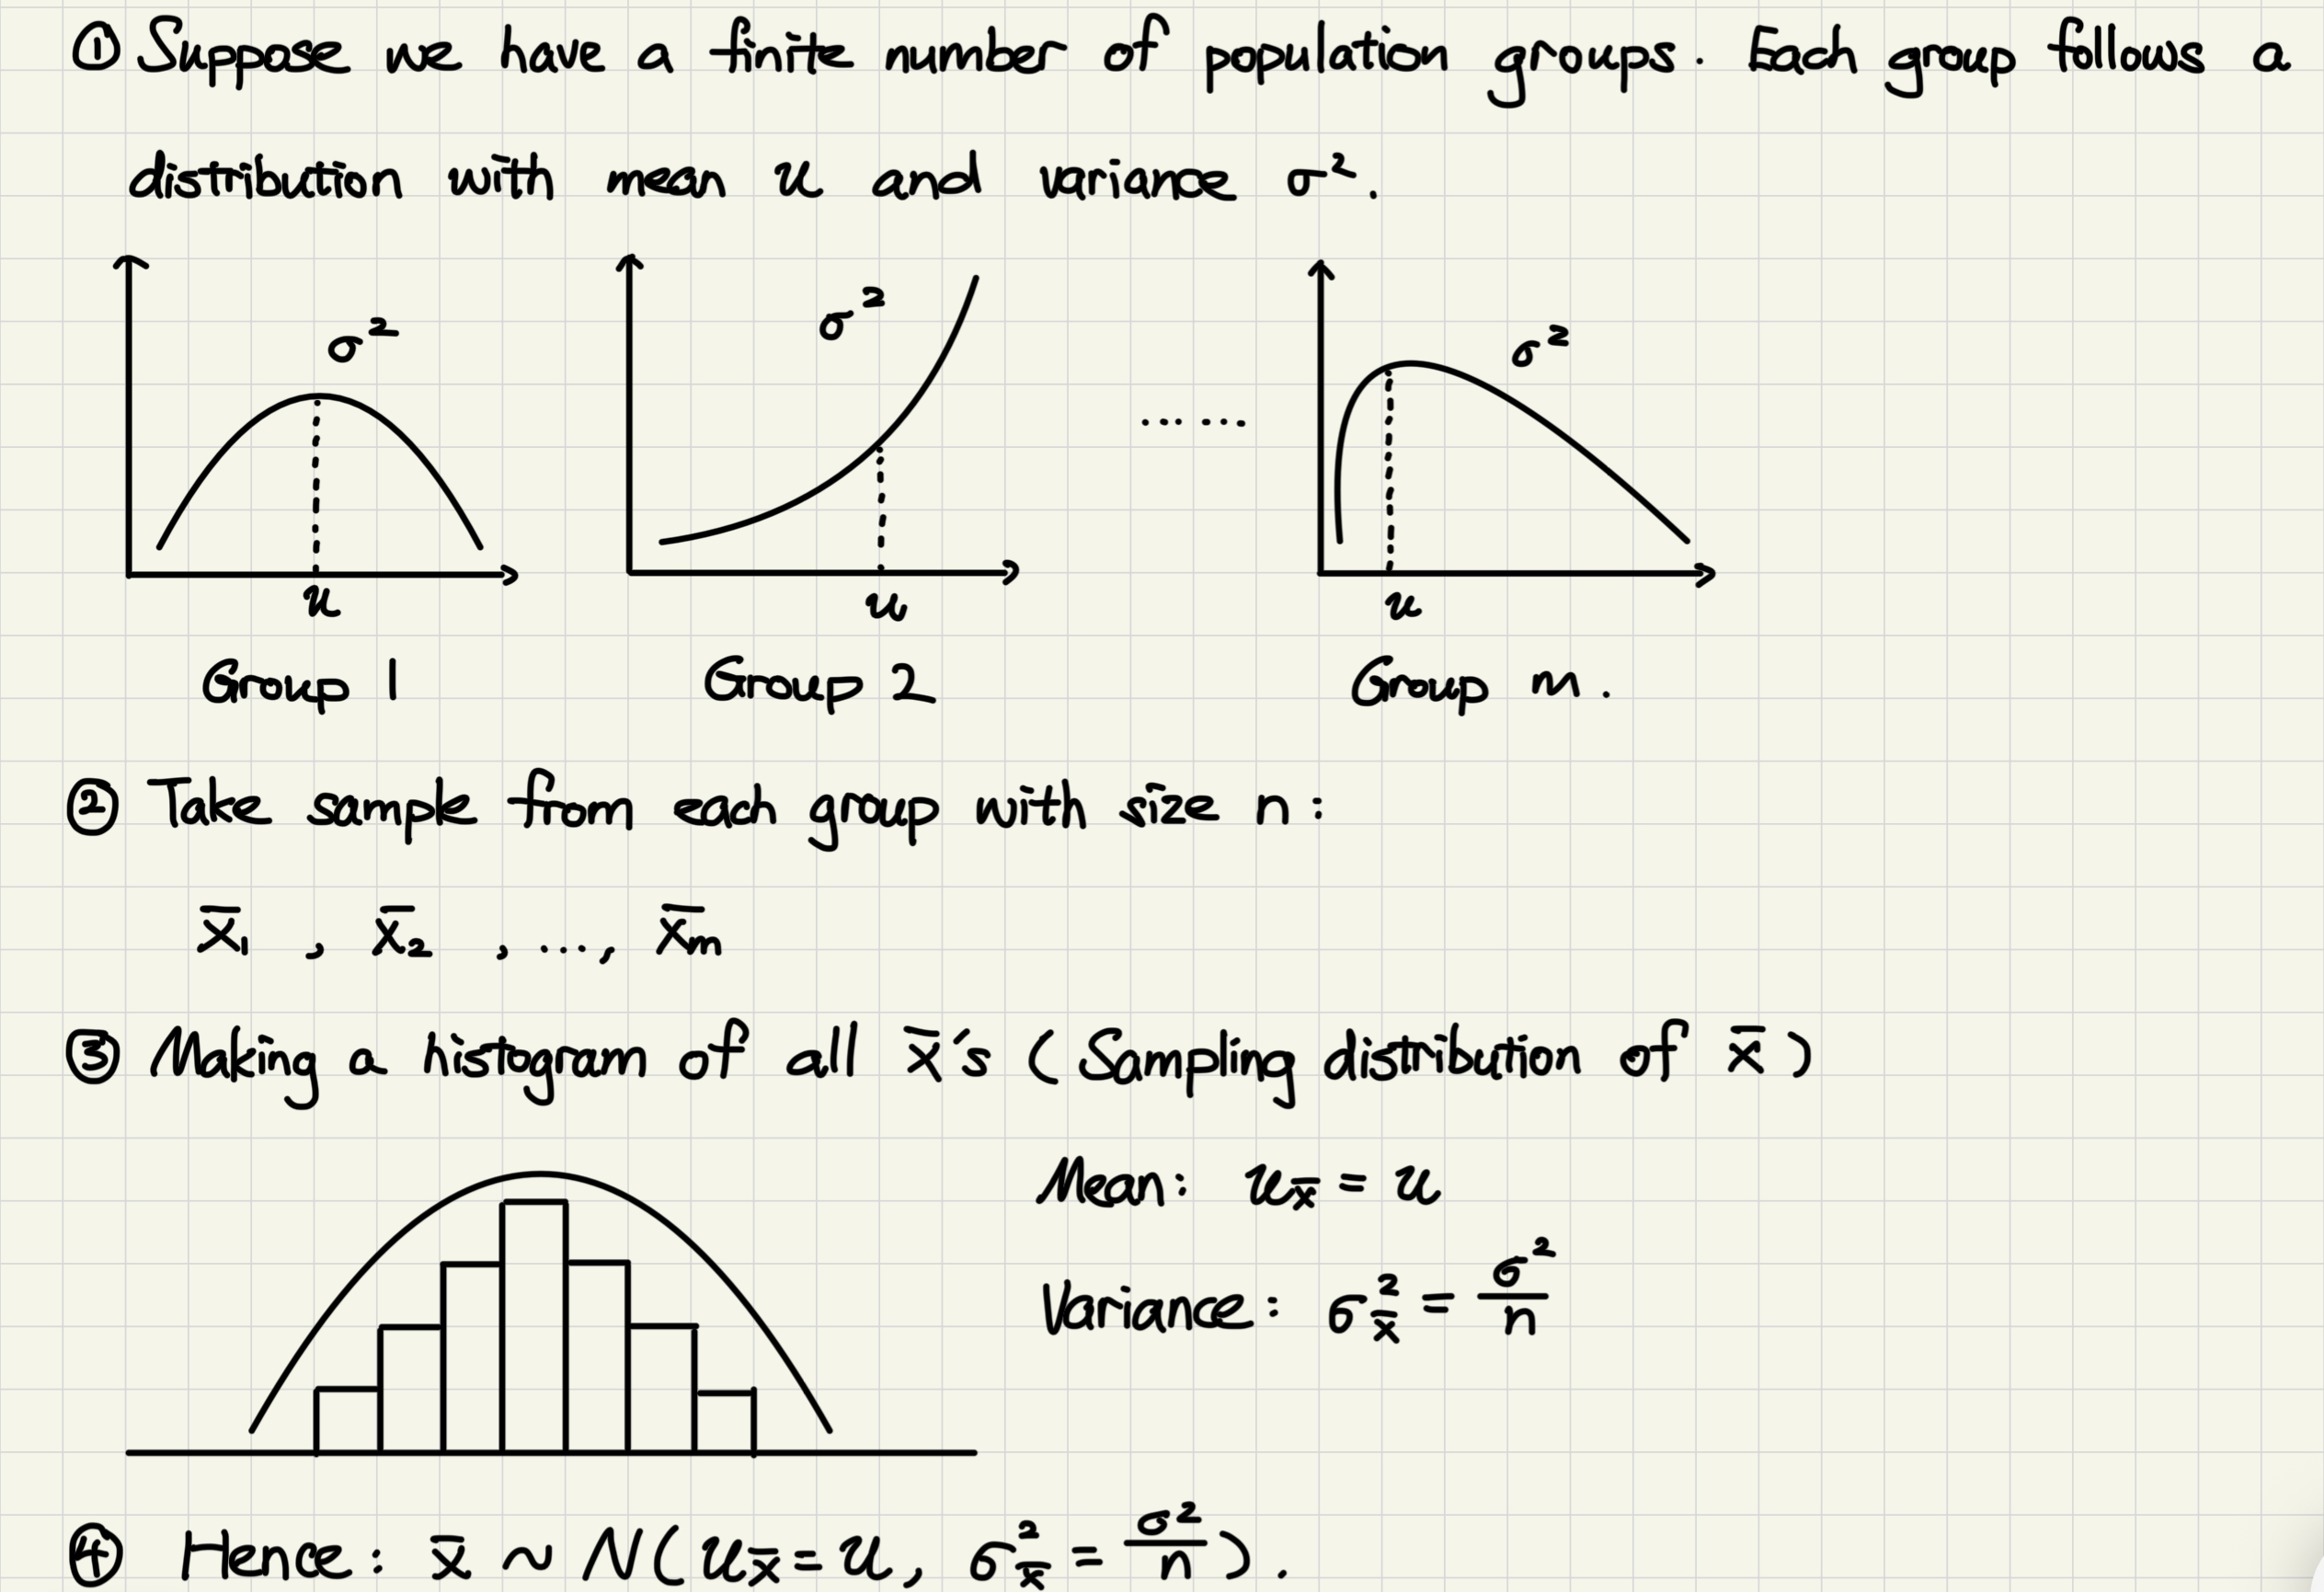
\includegraphics[scale=0.15]{Section3/Img3/CLT.jpg}
 \caption{Procedure of the Central Limit Theorem}
\end{figure}

\noindent
Now, let's begin with the proper definition of Central Limit Theorem.

\begin{definition}[Central Limit Theorem]
Let $X_1, X_2, ..., X_n$ be independent and identically distributed random variables with $E(X_i) = \mu$ and $Var(X_i) = \sigma^2 < \infty$. Then, we define the following: \[ U_{n} = \frac{\bar{X} - \mu}{(\frac{\sigma}{\sqrt{n}})} \sim N(\mu = 0, \sigma^2 = 1), \text{ where $\bar{X} = \frac{1}{n} \sum_{i =1}^{n}X_i$.}\]
Then the distribution function of $U_{n}$ converges to the standard Normal distribution function as $n \longrightarrow \infty$. That is, \[ \lim_{n\to\infty}P(U_n \le u) = \int_{\infty}^{u} \frac{1}{\sqrt{2\pi}} e^{-\frac{t^2}{2}}\,dt; \text{ for all u.}\]
\end{definition}

\noindent
For this course in particular, we do not need to pay that much attention to the proving part of the definition above. However, we use Central Limit Theorem to approximate distributions. Here are the two important approximations:

\begin{itemize}
	\item \[ \bar{X_n} \approx N(\mu, \frac{\sigma^2}{n});\]
	\item \[ T = \sum_{i = 1}^{n}X_i \approx N(n\mu, n\sigma^2).\]
\end{itemize}

\noindent
A reminder that the distribution of $U_n$ in definition $3.1$ and the two approximation of distribution above are extremely important in this course, until later chapters you may see some materials that are similar.
%\section{Practice Assignment 3}
%\label{ssec.ass3}
%\markright{\ref{ssec.ass3}
%\titleref{ssec.ass3}}
%\begin{enumerate}
\item Verify that: $$A^{-1}=\frac{1}{ad-bc}\left [
\begin{array}{rr} d&-b\\-c&a \end{array} \right ]$$ is the
correct formula for the inverse of $A$.

\noindent \textbf{Solution}

\noindent We can verify that $A^{-1}$ is the correct formula for
the inverse of $A$ by proving that $$AA^{-1}=I_{2}=A^{-1}A.$$
\noindent{\underline{Part 1:}}\ Prove $AA^{-1}=I_{2}$. \newline
Given $A= \left [\begin{array}{rr}a&b\\c&d \end{array} \right]$
and $A^{-1}=\dfrac{1}{ad-bc}
\left [\begin{array}{rr}d&-b\\-c&a\end{array} \right ]$. Then
\begin{align*}
AA^{-1} &= \left[\begin{array}{rr}
                         a&b\\
                         c&d \end{array} \right]
\left [\begin{array}{rr}\vspace{1mm}
                       \frac{d}{ad-bc}&\frac{-b}{ad-bc}\\ \vspace{1mm}
                      \frac{-c}{ad-bc}&\frac{a}{ad-bc} \end{array} \right]\\
&= \left[ \begin{array}{rr} \vspace{1mm}
                         \frac{ad-bc}{ad-bc}&\frac{-ab+ab}{ad-bc}\\ \vspace{1mm}
                         \frac{cd-cd}{ad-bc}&\frac{-bc+ad}{ad-bc} \end{array} \right] \\
&= \left[ \begin{array}{rr}
                        1&0\\
                        0&1 \end{array} \right]=I_{2}.
\end{align*}
{\underline{Part 2:}}\ Show that $A^{-1}A=I_{2}$.
\begin{align*}
A^{-1}A &= \left[ \begin{array}{ll} \vspace{1mm}
                       \frac{d}{ad-bc}&\frac{-b}{ad-bc}\\ \vspace{1mm}
                      \frac{-c}{ad-bc}&\frac{a}{ad-bc} \end{array} \right]
\left[ \begin{array}{ll}
                      a&b\\
                      c&d \end{array} \right] \\
&= \left[ \begin{array}{ll} \vspace{1mm}
                         \frac{ad-bc}{ad-bc}&\frac{db-bd}{ad-bc}\\ \vspace{1mm}
                         \frac{-ac+ac}{ad-bc}&\frac{-bc+ad}{ad-bc} \end{array} \right] \\
&= \left [\begin{array}{ll}
                        1&0\\
                        0&1 \end{array} \right ]=I_2
\end{align*}
\noindent Since $AA^{-1}=I_{2}=A^{-1}A$ we can say $A^{-1}$ is the
inverse of A.  From properties 3 and 4 in
section~\ref{ssec.propinv}, it is actually only necessary to show either Part 1 or Part 2 above.

\item Show that if $A$ and $B$ are invertible and the same size, then
$(AB)^{-1}=B^{-1}A^{-1}$. Hint: use the definition of an inverse.

\noindent \textbf{Solution}

Use the definition of an inverse and the fact that both
$A$ and $B$ are invertible. Then we must show that
$$
(AB)(B^{-1}A^{-1})=(B^{-1}A^{-1})(AB)=I
$$
{\underline{Proof:}}
\begin{align*}
(AB)(B^{-1}A^{-1})&=A(BB^{-1})A^{-1}\\
&=AIA^{-1}\\
&=AA^{-1}=I
\intertext{and}
(B^{-1}A^{-1})(AB)&=B^{-1}(A^{-1}A)B\\
&=B^{-1}IB\\
&=B^{-1}B=I.
\end{align*}
It then follows that $(AB)^{-1}=B^{-1}A^{-1}$.
\item Find the inverse of $\left [ \begin{array}{rrrrr}
                            a_{11}&0&0&0&0\\
                            0&a_{22}&0&0&0\\
                            0&0&a_{33}&0&0\\
                            0&0&0&a_{44}&0\\
                            0&0&0&0&a_{55} \end{array} \right ]$.

\noindent \textbf{Solution}

\noindent Assuming all $a_{ii}$'s do not equal zero the inverse
is:
\begin{eqnarray*}
\left [\begin{array}{rrrrr}
                        \frac{1}{a_{11}}&0&0&0&0\\
                        0&\frac{1}{a_{22}}&0&0&0\\
                        0&0&\frac{1}{a_{33}}&0&0\\
                        0&0&0&\frac{1}{a_{44}}&0\\
                        0&0&0&0&\frac{1}{a_{55}} \end{array} \right ]
\end{eqnarray*}

\item Find the inverse of the following matrices.

$\rm{(a)} \left [ \begin{array}{rr} -3&-8\\2&5 \end{array} \right
] \quad \quad  \rm{(b)} \left [ \begin{array}{rr} 4&-8\\-1&2
\end{array} \right ] \quad \quad \rm{(c)} \left [ \begin{array}{rr} 2&0\\-5&2\end{array}
\right ]$\\

\noindent \textbf{Solution}

\begin{description}\item (a) Using the formula we proved in Question \#$1$ of the
Assignment, the inverse of the matrix is:
\begin{eqnarray*}
\dfrac{1}{-15+16} \left[ \begin{array}{rr}5&8\\-2&-3 \end{array} \right]
=\left[ \begin{array}{rr}5&8\\-2&-3 \end{array} \right]
\end{eqnarray*}
\item (b)
\begin{eqnarray*}
\left |\begin{array}{rr}4&-8\\-1&2 \end{array} \right | = 8-8 = 0.
\end{eqnarray*}
\noindent Since the determinant is zero, you
can conclude that this matrix has no inverse.
\item (c)
\begin{eqnarray*}
\frac{1}{4-0} \left[ \begin{array}{rr}2&0\\5&2 \end{array} \right]= \left[ \begin{array}{rr}\frac{1}{2}&0\\\frac{5}{4}&\frac{1}{2} \end{array} \right]
\end{eqnarray*}
\end{description}
\item Find the inverse of the following matrices.

$\rm{(a)} \left [ \begin{array}{rrr} 2&1&0\\-4&1&1\\ 0&-2&-1
\end{array} \right ] \rm{(b)} \left [
\begin{array}{rrr} 3&0&0\\0&1&0\\ 0&0&-2\\ \end{array} \right ]$
$\rm{(c)} \left [ \begin{array}{rrr} 2&5&4\\5&-2&-1\\2&1&1\\
\end{array} \right ] \ \ \ \!\rm{(d)} \left [
\begin{array}{rrr} 2&1&8\\ 4&0&3\\-2&1&5 \end{array}  \right ]$\\

\noindent \textbf{Solution}

\begin{description} \item(a)
\begin{eqnarray*}
&&\left[ \begin{array}{rrrcrrr}2&1&0&\vline&1&0&0\\
                            -4&1&1&\vline&0&1&0\\
                             0&-2&-1&\vline&0&0&1
\end{array} \right]
\\&& \hspace{-12mm} \overset{\begin{smallmatrix}R_2+2R_1\\
\frac{1}{2}R_1\end{smallmatrix}}{\leadsto}
\left[ \begin{array}{rrrcrrr} 1&\frac{1}{2}&0&\vline&\frac{1}{2}&0&0\\
                               0&3&1&\vline&2&1&0\\
                               0&-2&-1&\vline&0&0&1
\end{array} \right]
\\&& \hspace{-12mm}
\overset{\begin{smallmatrix} \frac{1}{3}R_2\\R_3+2R_2\end{smallmatrix}}{\leadsto}
\left[ \begin{array}{rrrcrrr}1&\frac{1}{2}&0&\vline&\frac{1}{2}&0&0\\
                              0&1&\frac{1}{3}&\vline&\frac{2}{3}&\frac{1}{3}&0\\
                              0&0&-\frac{1}{3}&\vline&\frac{4}{3}&\frac{2}{3}&1
\end{array} \right]
\\&& \hspace{-12mm}
\overset{\begin{smallmatrix}R_{1}-\frac{1}{2}R_{2}\\-3R_3\end{smallmatrix}}{\leadsto}
\left[ \begin{array}{rrrcrrr}1&0&-\frac{1}{6}&\vline&\frac{1}{6}&-\frac{1}{6}&0\\
                              0&1&\frac{1}{3}&\vline&\frac{2}{3}&\frac{1}{3}&0\\
                              0&0&1&\vline&-4&-2&-3
\end{array} \right]
\\&& \hspace{-12mm}
\overset{\begin{smallmatrix}R_{2}-\frac{1}{3}R_{3}\\R_1+\frac{1}{6}R_3\end{smallmatrix}}{\leadsto}
\left[ \begin{array}{rrrcrrr}1&0&0&\vline&-\frac{1}{2}&-\frac{1}{2}&-\frac{1}{2}\\
                               0&1&0&\vline&2&1&1\\
                               0&0&1&\vline&-4&-2&-3
\end{array} \right]
\end{eqnarray*}
Then the matrix on the righthand side is the inverse.
\item (b)
$$
\left[ \begin{array}{rrr}
                       \frac{1}{3}&0&0\\
                       0&1&0\\
                       0&0&-\frac{1}{2}
\end{array} \right]
$$
\item (c)
$$
\left [\begin{array}{rrr}
                       1&1&-3\\
                       7&6&-22\\
                       -9&-8&29\
\end{array} \right]
$$
\item (d) Expand the determinant along the top row.
\begin{align*}
\left| \begin{array}{rrr} 2 & 1 & 8  \\ 4 & 0 & 3 \\ -2 & 1 & 5 \end{array} \right|
&= 2(-3) -1(20+6) + 8(4)\\
&= -6 -26 + 32 = 0.
\end{align*}
Since the determinant is zero, the matrix is not invertible.
\end{description}

\item Find the inverse of the following matrices.

$$
\rm {(a)} \left [ \begin{array}{rrrr} -1&0&2&0\\ 2&0&-1&0\\
0&-1&0&2\\ 0&2&0&-1\end{array} \right ] \quad \quad \rm {(b)}
\left [
\begin{array}{rrrr} 2&1&8&-2\\0&1&-1&2\\0&0&3&-1\\0&0&0&-1\end{array} \right ]
$$

$$\ \rm {(c)} \left [ \begin{array}{rrrr}
-1&4&1&0\\2&0&0&3\\1&-1&-3&2\\0&1&14&-4\end{array} \right ] \quad
\quad \rm {(d)} \left [ \begin{array}{rrrr} 1&0&3&-2\\ 1&0&1&2\\
4&6&2&8\\ 1&0&-1&7\end{array} \right ].
$$

\noindent \textbf{Solution}

\begin{description}
\item (a)
$$ \left [\begin{array}{rrrr}
                       \frac{1}{3}&\frac{2}{3}&0&0\\
                       0&0&\frac{1}{3}&\frac{2}{3}\\
                       \frac{2}{3}&\frac{1}{3}&0&0\\
                       0&0&\frac{2}{3}&\frac{1}{3}\end{array} \right ]
$$
\item (b)
$$
\left[ \begin{array}{rrrr}\vspace{1mm}
                       \frac{1}{2}&-\frac{1}{2}&-\frac{3}{2}&-\frac{1}{2}\\ \vspace{1mm}
                       0&1&\frac{1}{3}&\frac{5}{3}\\ \vspace{1mm}
                       0&0&\frac{1}{3}&-\frac{1}{3}\\
                       0&0&0&-1
\end{array} \right]
$$
\item (c) Expand the determinant along the second row.
\begin{align*}
\left| \begin{array}{rrrr} -1 & 4 & 1 & 0 \\ 2 & 0 & 0 & 3 \\ 1 & -1 & -3 & 2 \\ 0 & 1 & 14 & -4 \end{array} \right|
&= -2 \left| \begin{array}{rrr} 4 & 1 & 0 \\ -1 & -3 & 2 \\ 1 & 14 & -4 \end{array} \right| +
3 \left| \begin{array}{rrr} -1 & 4 & 1 \\ 1 & -1 & -3 \\ 0 & 1 & 14 \end{array} \right| \\
&= -2 \bigl[ 4(12-28) - (4-2) \bigr] + 3\bigl[-1(3-1) + 14(1-4) \bigr] \\
&= -2[-64-2] + 3[-2-42]\\
&= 132 - 132 = 0.
\end{align*}
Hence the matrix is singular.
\item (d)
$$
\left[ \begin{array}{rrrr} \vspace{1mm}
                       -\frac{9}{2}&\frac{19}{2}&0&-4\\ \vspace{1mm}
                       \frac{5}{6}&-\frac{13}{6}&\frac{1}{6}&\frac{2}{3}\\ \vspace{1mm}
                       \frac{5}{2}&-\frac{9}{2}&0&2\\
                       1&-2&0&1
\end{array} \right]
$$
\end{description}

\item For what values of $a$ does $A^{-1}$ fail to exist?
\begin{align*}
&\rm{(a)}\ A= \left [ \begin{array}{rr} 3&a\\-4&5 \end{array}
\right ] &\rm{(b)}\ A&=\left [\begin{array}{rc}
-3&(1+a)\\a&-2\end{array} \right]\\
&\rm{(c)}\ A= \left [ \begin{array}{rcc}
-1&(4+a)&\frac{1}{2}\\0&(a-5)&3\\ 0&0&-3a \end{array} \right]
&\rm{(d)}\ A&= \left [ \begin{array}{crc}
3a&1&0\\2&2&(a+1)\\1&0&1 \end{array} \right ].
\end{align*}

\noindent \textbf{Solution}

\begin{description}
\item (a)
\begin{align*}
\left| \begin{array}{rr} 3 & a \\ -4 & 5 \end{array} \right| = 15 + 4a = 0
\quad \mathrm{when}\ a = \tfrac{-15}{4}.
\end{align*}
Hence if $a= \tfrac{-15}{4}$, $A$ is not invertible (singular).
\item (b)
\begin{align*}
\left| \begin{array}{rr} -3 & 1+a \\ a & -2 \end{array} \right| &= 6 - a(1+a)\\
&= -a^2 - a + 6 = -(a+3)(a-2) \\
&= 0 \quad \mathrm{when}\ a=2,\ -3.
\end{align*}
Hence if $a = 2$ or $-3$, $A$ is singular.
\item (c)
Expanding down the first column,
\begin{align*}
\det{(A)} &= - \left| \begin{array}{rr} a-5 & 3 \\ 0 & -3a \end{array} \right| \\
&= 3a(a-5) = 0 \quad \mathrm{when}\ a = 0,\,5.
\end{align*}
Hence if $a=0$ or $5$, $A$ is singular.
\item (d)
Expanding along the top row,
\begin{align*}
\det{(A)} &= 3a \left| \begin{array}{rr} 2 & (a+1) \\ 0 & 1 \end{array} \right|
- \left| \begin{array}{rr} 2 & (a+1) \\ 1 & 1 \end{array} \right|\\
&= 6a - (2 - (a+1))\\
&= 7a - 1\\
&= 0 \quad \mathrm{when}\ a = \tfrac{1}{7}.
\end{align*}
Hence when $a=\tfrac{1}{7}$, $A$ is singular.
\end{description}

\item For the following system:
$$\begin{array}{rrr} 2x_1-2x_2+3x_3&=&3\\ 2x_3-x_4&=&-1\\
4x_1+5x_2+2x_3&=&1\\ x_3+2x_4&=&-3 \end{array},$$
\begin{enumerate}
\item Set up the system as $A{\bf x}={\bf b}$.
\item Find $A^{-1}.$
\item Find the solution.
\item Let ${\bf b}_1=[ \ 2 \ 0 \ 1 \ 0 \ ]^t$. Find the solution
to $A{\bf x}={\bf  b}_1$.
\item What is the solution to $A{\bf x}={\bf 0}$?
\end{enumerate}

\noindent \textbf{Solution}
\begin{description} \item (a)
$$ \left [\begin{array}{rrrr}
                       2&-2&3&0\\
                       0&0&2&-1\\
                       4&5&2&0\\
                       0&0&1&2\end{array} \right ]
\left [\begin{array}{r}
                       x_{1}\\
                       x_{2}\\
                       x_{3}\\
                       x_{4}\end{array} \right ]  =
\left [\begin{array}{r}
                       3\\
                       -1\\
                       1\\
                       -3\end{array} \right ]
$$
\item (b)
$$
A^{-1}= \left[ \begin{array}{rrrr} \vspace{1mm}
                       \frac{5}{18}&-\frac{19}{45}&\frac{1}{9}&-\frac{19}{90}\\ \vspace{1mm}
                       -\frac{2}{9}&\frac{8}{45}&\frac{1}{9}&\frac{4}{45}\\ \vspace{1mm}
                       0&\frac{2}{5}&0&\frac{1}{5}\\
                       0&-\frac{1}{5}&0&\frac{2}{5}\end{array} \right]
$$
\item (c)
\begin{align*}
{\bf x}&=A^{-1}{\bf b}\\
\left[ \begin{array}{r}x_{1}\\
                       x_{2}\\
                       x_{3}\\
                       x_{4}
\end{array} \right ] &=
\left[ \begin{array}{rrrr} \vspace{1mm}
                       \frac{5}{18}&-\frac{19}{45}&\frac{1}{9}&-\frac{19}{90}\\ \vspace{1mm}
                       -\frac{2}{9}&\frac{8}{45}&\frac{1}{9}&\frac{4}{45}\\ \vspace{1mm}
                       0&\frac{2}{5}&0&\frac{1}{5}\\
                       0&-\frac{1}{5}&0&\frac{2}{5}
\end{array} \right]
\left[ \begin{array}{r} 3\\
                       -1\\
                       1\\
                       -3
\end{array} \right] \\
\left [\begin{array}{r}x_{1}\\
                       x_{2}\\
                       x_{3}\\
                       x_{4}
\end{array} \right ] &=
\left[ \begin{array}{r} 2\\
                       -1\\
                       -1\\
                       -1
\end{array} \right]
\end{align*}
\item (d)
Rearrange to get ${\bf x}=A^{-1}{\bf b_{1}}$. Examine.
\begin{align*}
\left[ \begin{array}{r}
                       x_{1}\\
                       x_{2}\\
                       x_{3}\\
                       x_{4}\end{array} \right]
&=
\left[ \begin{array}{rrrr} \vspace{1mm}
                       \frac{5}{18}&-\frac{19}{45}&\frac{1}{9}&-\frac{19}{90}\\ \vspace{1mm}
                       -\frac{2}{9}&\frac{8}{45}&\frac{1}{9}&\frac{4}{45}\\ \vspace{1mm}
                       0&\frac{2}{5}&0&\frac{1}{5}\\
                       0&-\frac{1}{5}&0&\frac{2}{5}\end{array} \right]
\left[ \begin{array}{r}
                       2\\
                       0\\
                       1\\
                       0
\end{array} \right] \\
\left[ \begin{array}{r}x_{1}\\
                       x_{2}\\
                       x_{3}\\
                       x_{4}
\end{array} \right]&=
\left[ \begin{array}{r}\vspace{1mm} \frac{2}{3}\\
                        -\frac{1}{3}\\
                       0\\
                       0\end{array} \right]
\end{align*}
\item (e)
$A$ is invertible, so the solution to the homogeneous
system is ${\bf 0 }$. Observe: $A{\bf x}={\bf 0}$.
Rearrange to get ${\bf x}=A^{-1}{\bf 0}$.
\begin{align*}
\left[ \begin{array}{r}x_{1}\\
                       x_{2}\\
                       x_{3}\\
                       x_{4}
\end{array} \right] &=
\left[ \begin{array}{rrrr}\vspace{1mm}
                       \frac{5}{18}&-\frac{19}{45}&\frac{1}{9}&-\frac{19}{90}\\ \vspace{1mm}
                       -\frac{2}{9}&\frac{8}{45}&\frac{1}{9}&\frac{4}{45}\\ \vspace{1mm}
                       0&\frac{2}{5}&0&\frac{1}{5}\\
                       0&-\frac{1}{5}&0&\frac{2}{5}
\end{array} \right]
\left [\begin{array}{r}0\\
                       0\\
                       0\\
                       0
\end{array} \right]\\
\left[ \begin{array}{r}x_{1}\\
                       x_{2}\\
                       x_{3}\\
                       x_{4}
\end{array} \right ] &=
\left[ \begin{array}{r}0\\
                       0\\
                       0\\
                       0
\end{array} \right]
\end{align*}
\end{description}

\item For the following system:
$$
\begin{array}{rrr} x_1+3x_3+2x_4&=&4\\
                   2x_1-x_2+8x_3&=&3\\
                   3x_1+2x_2+4x_3+3x_4&=&1\\
                   2x_1+3x_2-x_3+5x_4&=&2
\end{array}
$$
\begin{enumerate}
\item Set up the system as $A{\bf x}={\bf b}$.
\item Find $A^{-1}.$
\item Find the solution.
\item Let ${\bf b}_1=[ \ 1 \ -1 \ 0 \ 2 \ ]^t$. Find the solution
to $A{\bf x}={\bf  b}_1$.
\item What is the solution to $A{\bf x}={\bf 0}$?
\end{enumerate}

\noindent \textbf{Solution} \begin{description} \item (a)
$$
\left[ \begin{array}{rrrr}
                       1&0&3&2\\
                       2&-1&8&0\\
                       3&2&4&3\\
                       2&3&-1&5
\end{array} \right]
\left[ \begin{array}{r}x_{1}\\
                       x_{2}\\
                       x_{3}\\
                       x_{4}
\end{array} \right] =
\left [\begin{array}{r}4\\
                       3\\
                       1\\
                       2\end{array} \right]
$$
\item (b)
The matrix is not invertible.
\item (c)
Write system as an augmented matrix in reduced
row-echelon form since we cannot use the inverse:
$$
\left[ \begin{array}{rrrr|r}
                         1&0&0&-31&-59\\
                         0&1&0&26&47\\
                         0&0&1&11&21\\
                         0&0&0&0&0
\end{array} \right]
$$
Let $x_4=s$.  Then $x_3=21-11s,\ x_2=47-26s$, and
$x_1=-59+31s$.
\item (d)
Write the system as an augmented matrix and row-reduce
to solve.
$$
\left[ \begin{array}{rrrr|r}
                         1&0&0&-31&-26\\
                         0&1&0&26&21\\
                         0&0&1&11&9\\
                         0&0&0&0&0
\end{array} \right]
$$
Let $x_4=s$.  Then $x_3=9-11s,\ x_2=21-26s$, and
$x_1=-26+31s$.
\item (e)
Notice that you may already use the matrix in
row-reduced echelon form with the last column containing all zero
entries.
$$
\left[ \begin{array}{rrrr|r}
                         1&0&0&-31&0\\
                         0&1&0&26&0\\
                         0&0&1&11&0\\
                         0&0&0&0&0
\end{array} \right]
$$
Let $x_4=s$.  Then $x_3=-11s,\ x_2=-26s$, and $x_1=31s$.
\end{description}

\item For
$$
A=\left[ \begin{array}{rrr} 1&5&2\\ -3&4&1\\-1&2&0 \end{array}
\right ], \quad B=\left [ \begin{array}{rrr} 2&5&-1\\ 2&-3&1\\
6&-1&1 \end{array} \right ] \mbox{\ and\ } C=\left [
\begin{array}{rrr} 0&3&1\\ -2&0&3\\ 4&2&0 \end{array} \right ],$$
find
\begin{enumerate}
\item (i) det($A$) \quad (ii) det($B$) \quad (iii) det($C$)
\item (i) det($AC$) \quad (ii) det($AB$) \quad (iii) det($BC$)
\item (i) det($A$)+det($B$) \quad (ii) det($A+B$)
\item (i) det($2A$) \quad (ii) 2det($A$)
\item (i) det($C^t$) \quad (ii) det($CA^t$)
\item det($C^{-1}$)
\end{enumerate}

\noindent \textbf{Solution} \begin{description}
\item (a) (i)
Expand along the top row
\begin{align*}
\left| \begin{array}{rrr} 1 & 5 & 2\\ -3 & 4 & 1 \\ -1 & 2 & 0 \end{array} \right|
&= 1(0-2) -5(0+1) + 2(-6+4)\\
&= -2-5-4 = -11.
\end{align*}
\item \quad\, (ii) \begin{align*}
\left| \begin{array}{rrr} 2 & 5 & -1 \\ 2 & -3 & 1 \\ 6 & -1 & 1 \end{array} \right|
&= \left| \begin{array}{rrr} 8 & 4 & 0 \\ -4 & -2 & 0 \\ 6 & -1 & 1 \end{array} \right| \quad \begin{array}{r} R_1 + R_3 \\ R_2 - R_3 \end{array}\\
&= 4 \left| \begin{array}{rrr} 2 & 1 & 0 \\ -4 & -2 & 0 \\ 6 & -1 & 1 \end{array} \right|\\
&= 4(-2) \left| \begin{array}{rrr} 2 & 1 & 0 \\ 2 & 1 & 0\\ 6 & -1 & 1 \end{array} \right| \\
&= 0 \quad \mathrm{(2\ rows\ the\ same)}.
\end{align*}
\item \quad\,  (iii)
Expand along the top row:
\begin{align*}
\left| \begin{array}{rrr} 0 & 3 & 1 \\ -2 & 0 & 3 \\ 4 & 2 & 0 \end{array} \right| &=
-3 \left| \begin{array}{rr} -2 & 3 \\ 4 & 0 \end{array} \right| + \left| \begin{array}{rr} -2 & 0 \\ 4 & 2 \end{array} \right|\\
&= -3(-12) + (-4) = 32.
\end{align*}

\item (b) (i)
det$(AC)\ =\ $det$(A)$det$(C)\ =\ (-11)(32)\ =\ -352$\\
\item \quad\, (ii)
det$(AB)\ =\ $det$(A)$det$(B)\ =\ (-11)(0)\ =\ 0$\\
\item \quad\, (iii)
det$(BC)\ =\ $det$(B)$det$(C)\ =\ (0)(32)\ =\ 0$\\
\item (c) (i)
det$(A)+$det$(B)\ =\ (-11)+(0)\ =\ -11$\\
\item \quad\, (ii)
det$(A+B)\ =\ \left | \begin{array}{rrr}
                        3&10&1\\
                        -1&1&2\\
                        5&1&1 \end{array} \right |\ =\ 101$\\
\item (d) (i)
det$(2A)\ =\ 2^3$det$(A)\ =\ 8(-11)\ =\ -88$\\
\item \quad\, (ii)
$2$det($A$)$=2(-11)=-22$\\
\item (e) (i)
det$(C^t)\ =\ $det$(C)\ =\ 32$\\
\item \quad\, (ii)
det$(CA^t)\ =\ $det$(C)$det$(A^t)\ =\ $det$(C)$det$(A)\ =\
(32)(-11)\ =\ -352$\\
\item (f)
det($C^{-1}$)$=\frac{1}{32}$ which is the reciprocal of det($C$).
\end{description}

\item Find the determinant of the following matrices.
\begin{align*}
&\mathrm{(a)} \left[ \begin{array}{rr} 6&3\\-2&0 \end{array} \right]&
&\mathrm{(b)} \left[ \begin{array}{rr} 1&-2\\-2&4\end{array} \right]&
&\mathrm{(c)} \left[ \begin{array}{rr} 7&8\\-1&5 \end{array} \right]\\
&\mathrm{(d)} \left[ \begin{array}{rr} a&5\\ a&-1\end{array} \right]&
&\mathrm{(e)} \left[ \begin{array}{cc} (b-1)&-1\\ 3&(b+2) \end{array} \right]&
&\mathrm{(f)} \left[ \begin{array}{cc} a&(a+b)\\(b-a)&b \end{array} \right]
\end{align*}

\noindent \textbf{Solution} \begin{description} \item (a)
\begin{align*}
\left| \begin{array}{rr} 6&3\\-2&0 \end{array} \right| &=a_{11}\,a_{22}-a_{12}\,a_{21}\\
&=(6)(0)-(3)(-2)\\&
=0+6=6
\end{align*}
\item (b)
\begin{align*}
\left| \begin{array}{rr} 1&-2\\-2&4\end{array} \right | &=a_{11}\,a_{22}-a_{12}\,a_{21} \\
&=(1)(4)-(-2)(-2)\\
&=4-4=0
\end{align*}
\item (c)
\begin{align*}
\left| \begin{array}{rr} 7&8\\-1&5 \end{array} \right | &=a_{11}\,a_{22}-a_{12}\,a_{21}  \\
&=(7)(5)-(8)(-1)\\
&=35+8=43
\end{align*}
\item (d)
\begin{align*}
\left| \begin{array}{rr} a&5\\ a&-1\end{array} \right| &= a_{11}\,a_{22}-a_{12}\,a_{21} \\
&=(a)(-1)-(5)(a)=-6a
\end{align*}
\item (e)
\begin{align*}
\left| \begin{array}{cc} (b-1)&-1\\ 3&(b+2) \end{array} \right|& =a_{11}\,a_{22}-a_{12}\,a_{21}\\
&=(b-1)(b+2)-(-1)(3)\\
&=(b^2+b-2)+3=b^2+b+1
\end{align*}
\item (f)
\begin{align*}
\left| \begin{array}{cc} a&(a+b)\\(b-a)&b \end{array} \right | &=a_{11}\,a_{22}-a_{12}\,a_{21} \\
&=(a)(b)-(a+b)(b-a)\\
&=ab-(b^{2}-a^{2})=a^2+ab-b^2
\end{align*}
\end{description}

\item Find the determinant of the following matrices.
\begin{align*}
&\mathrm{(a)} \left[ \begin{array}{rrr} 2&0&1\\ 4&-5&1 \\ 0&3&2 \end{array} \right]&
&\mathrm{(b)} \left[ \begin{array}{rrr} 5&7&2\\-3&6&5\\ 2&1&-1\end{array} \right]&
&\mathrm{(c)} \left[ \begin{array}{rrr} 1&6&-1\\-1&-2&1 \\ 3&1&-3\end{array} \right ]\\
&\mathrm{(d)} \left[ \begin{array}{rrr} 2&0&0\\ b&3&b\\ 1&-1&3 \end{array} \right]&
&\mathrm{(e)} \left[ \begin{array}{crr} 2a&0&1\\ (a-3)&5&4\\ 2&0&-a \end{array} \right]&
&\mathrm{(f)} \left [ \begin{array}{ccc} a&2&-3\\(a+2)&a^2&3\\0&1&(a-1)\end{array} \right]
\end{align*}

\noindent \textbf{Solution} \begin{description} \item (a)
Expand along the top row
\begin{align*}
\begin{vmatrix} 2&0&1\\ 4&\!\!\!-5&1 \\ 0&3&2 \end{vmatrix} &= 2 \left| \begin{array}{rr}-5 & 1\\3 & 2\end{array} \right| +
\left| \begin{array}{rr} 4 & -5 \\ 0 & 3 \end{array} \right| \\
&= 2(-10-3) + 12 \\
&= -26 + 12 = -14.
\end{align*}
\item (b)
Expand along the top row
$$
\left| \begin{array}{rrr} 5&7&2\\-3&6&5\\ 2&1&-1\end{array} \right| = -36
$$
\item (c)
\begin{align*}
\left| \begin{array}{rrr} 1&6&-1\\-1&-2&1 \\ 3&1&-3\end{array} \right| &=
\left| \begin{array}{rrr} 0 & 4 & 0\\-1 & -2 & 1\\0 & -5 & 0 \end{array} \right| \quad \begin{array}{r} R_1 + R_2 \\ \ \\ R_3 + 3R_2 \end{array}\\
&= 0.
\end{align*}
\item (d)
Expand along the top row
$$
\left| \begin{array}{rrr} 2&0&0\\ b&3&b\\ 1&-1&3 \end{array} \right|=18+2b
$$
\item (e)
Expand down the middle column
$$
\left|\begin{array}{crr} 2a&0&1\\ (a-3)&5&4\\ 2&0&-a \end{array} \right|=-10a^{2}-10
$$
\item (f)
Expand down the first column
\begin{align*}
\left| \begin{array}{ccc} a&2&-3\\(a+2)&a^2&3\\0&1&(a-1)\end{array} \right| &= a\left| \begin{array}{rr} a^2 & 3 \\ 1 & (a-1) \end{array} \right|
- (a+2) \left| \begin{array}{rr}2 & -3 \\1 & (a-1) \end{array} \right|\\
&= a(a^3 - a^2 - 3) - (a+2)(2a-2+3)\\
&= a^4 - a^3 - 3a - (2a^2 + 5a + 2)\\
&= a^4 - a^3 - 2a^2 - 8a - 2.
\end{align*}
\end{description}

\item Find the determinant of the following matrices.
\begin{align*}
&\mathrm{(a)} \left[ \begin{array}{rrrr} 2&1&0&0\\ 3&2&1&4\\-1&1&0&2\\8&1&0&3 \end{array} \right]&
&\mathrm{(b)} \left[ \begin{array}{rrrr} 3&0&2&1\\4&-7&7&5\\3&-6&4&8\\2&1&-1&4 \end{array} \right]\\
&\mathrm{(c)} \left[ \begin{array}{rrrr} 0&3&1&3\\-1&0&2&1\\2&1&0&-1\\3&-2&2&0\end{array} \right]&
&\mathrm{(d)} \left[ \begin{array}{rrrr} 1&0&3&5\\4&2&-1&6\\0&0&4&0\\-7&2&0&5\end{array} \right]
\end{align*}\\
\noindent \textbf{Solution} 

\begin{description} \item (a)
Expand down the third column
\begin{align*}
\left| \begin{array}{rrrr}2&1&0&0\\ 3&2&1&4\\-1&1&0&2\\ 8&1&0&3 \end{array} \right| &=
- \left| \begin{array}{rrr}2 & 1 & 0 \\ -1 & 1 & 2 \\ 8 & 1 & 3 \end{array} \right| \\
&= -\bigl[2(3-2) - (-3-16)\bigr] \\
&=-(2+19) = -21.
\end{align*}
\item (b)
\noindent The determinant is 0.
\item (c)
\noindent The determinant is 55.
\item (d)
\noindent The determinant is 432.
\end{description}

\item Find the determinants of
\begin{align*}
\mathrm{(a)}\ A& =\left[ \begin{array}{rrr}0&0&a_{13}\\0&a_{22}&a_{23}\\a_{31}&a_{32}&a_{33} \end{array} \right]&
\mathrm{(b)}\ A&=\left[ \begin{array}{rrrr}0&0&0&a_{14}\\0&0&a_{23}&a_{24}\\0&a_{32}&a_{33}&a_{34}\\a_{41}&a_{42}&a_{43}&a_{44} \end{array} \right]\\
\mathrm{(c)}\ A&=\left[ \begin{array}{rrrrr}0&0&0&0&a_{15}\\0&0&0&a_{24}&a_{25}\\0&0&a_{33}&a_{34}&a_{35}\\
0&a_{42}&a_{43}&a_{44}&a_{45}\\ a_{51}&a_{52}&a_{53}&a_{54}&a_{55} \end{array}\right]
\end{align*}

\noindent \textbf{Solution} 

\begin{description}\item (a)
Expand along the top row
\begin{align*}
\det(A) = \left| \begin{array}{rrr}0&0&a_{13}\\0&a_{22}&a_{23}\\a_{31}&a_{32}&a_{33} \end{array} \right|
= a_{13} \left| \begin{array}{rr} 0 & a_{22} \\ a_{31} & a_{32} \end{array} \right| = - a_{13}a_{31}a_{22}.
\end{align*}

\item (b)
Expand along the top row
\begin{align*}
\det(A)= \left| \begin{array}{rrrr}0&0&0&a_{14}\\0&0&a_{23}&a_{24}\\0&a_{32}&a_{33}&a_{34}\\a_{41}&a_{42}&a_{43}&a_{44} \end{array} \right|
&= -a_{14} \left| \begin{array}{rrr} 0 & 0 & a_{23} \\ 0 & a_{32} & a_{33} \\ a_{41} & a_{42} & a_{43} \end{array} \right| \\
&= a_{14}a_{23}a_{32}a_{41} \quad \mathrm{using\ (a)}.
\end{align*}

\item (c)
Expand along the top row and use (b)
\begin{align*}
\det(A) = \left| \begin{array}{rrrrr}
                        0&0&0&0&a_{15}\\
                        0&0&0&a_{24}&a_{25}\\
                        0&0&a_{33}&a_{34}&a_{35}\\
                        0&a_{42}&a_{43}&a_{44}&a_{45}\\
                        a_{51}&a_{52}&a_{53}&a_{54}&a_{55} \end{array} \right | =
a_{15}\,a_{24}\,a_{33}\,a_{42}\,a_{51}.
\end{align*}
\end{description}

\item Assume that $$\left | \begin{array}{rrr}
a&b&c\\d&e&f\\g&h&i \end{array} \right |=1.$$ Find the
determinants of the following matrices.
\begin{align*}
&\mathrm{(a)} \left[ \begin{array}{rrr} 5a&5b&5c\\5d&5e&5f\\5g&5h&5i \end{array} \right]&
&\mathrm{(b)} \left[ \begin{array}{rrr} d&e&f\\ a&b&c \\g&h&i \end{array} \right ]\\
&\mathrm{(c)} \left[ \begin{array}{rrr} -a&-b&-c\\ d&e&f\\ 3g&3h&3i\end{array} \right ]&
&\mathrm{(d)} \left[ \begin{array}{ccc} (a-d)&(b-e)&(c-f)\\ d&e&f\\ 2g&2h&2i\end{array}\right]\\
&\mathrm{(e)} \left[ \begin{array}{ccc} -d&-e&-f\\ a&b&c\\ (g+4a)&(h+4b)&(i+4c) \end{array} \right ]&
&\mathrm{(f)} \ 4\left[ \begin{array}{rrr} a&b&c\\d&e&f\\g&h&i \end{array} \right]^{-1}
\end{align*}\\

\noindent \textbf{Solution} \begin{description}\item (a)
\begin{align*}
\begin{vmatrix}5a&5b&5c\\5d&5e&5f\\5g&5h&5i \end{vmatrix}
&=(5)(5)(5) \begin{vmatrix}a&b&c\\d&e&f\\g&h&i \end{vmatrix}\\
&=5^3(1)\\
&=125
\end{align*}
\item (b)
\begin{align*}
\begin{vmatrix}d&e&f\\ a&b&c \\g&h&i \end{vmatrix}
&=(-1)\begin{vmatrix}a&b&c\\d&e&f\\g&h&i \end{vmatrix}\\
&=(-1)(1)\\
&=-1
\end{align*}
\item (c)
\begin{align*}
\left| \begin{array}{rrr}-a&-b&-c\\ d&e&f\\ 3g&3h&3i \end{array} \right|
&=(-1)(3)\left | \begin{array}{rrr}a&b&c\\d&e&f\\g&h&i \end{array} \right|\\
&=(-1)(3)(1)\\
&=-3
\end{align*}
\item (d)
\begin{align*}
\left| \begin{array}{rrr}(a-d)&(b-e)&(c-f)\\ d&e&f\\ 2g&2h&2i \end{array} \right|
\ \ \overset{R_{1}+R_{2}}{\leadsto} \ \
(2)\begin{vmatrix}a&b&c\\ d&e&f\\ g&h&i \end{vmatrix} = 2
\end{align*}
\item (e)
\begin{align*}
\left| \begin{array}{ccc}-d&-e&-f\\a&b&c\\(g+4a)&(h+4b)&(i+4c)\end{array} \right|
&=(-1)(-1) \begin{vmatrix}a&b&c\\d&e&f\\g&h&i \end{vmatrix}\\
&=(-1)(-1)(1)\\
&=1
\end{align*}
\item (f)
$$
\det(4A^{-1})=4^3(1)=64
$$
\end{description}

\item Find all values of $b$ for which the following matrices fail to be invertible.
\begin{align*}
\mathrm{(a)}\ \left[ \begin{array}{rrr} 2&1&0\\-b&3&4\\-1&3b&-1 \end{array} \right] &
&\mathrm{(b)}\ \left[ \begin{array}{crc}(b+3)&3&-1\\0&-b&(2-b)\\1&1&0\end{array} \right] &
&\mathrm{(c)}\ \left[ \begin{array}{crcr} 1&0&2&3\\(b+2)&-b&b&0\\0&2&5b&1\\0&0&(3-b)&0 \end{array} \right]
\end{align*}
\noindent The matrices fail to be invertible when the determinant
equals zero.\\

\noindent \textbf{Solution} \begin{description}\item (a)
The determinant is $-10-25b$.  Setting it equal to zero,
we get $b=-\frac{2}{5}$ so that the matrix is not invertible.
\item (b)
The determinant is $b^2-3b$.  Setting it equal to zero,
we get $b=0,3$ so that the matrix is not invertible.
\item (c) The determinant is $5b^2-3b-36$.  Setting it equal to
zero, we get $b=3,-\tfrac{12}{5}$ so that the matrix is not invertible.
\end{description}

\item For the following homogeneous systems,
\ \

{\rm (i.)}$\begin{array}{rrl} 2x_1+x_2+3x_4&=&0\\ 3x_1+2x_2&=&0\\
5x_1-x_2-2x_3&=&0\\ 3x_2-x_3&=&0 \end{array}$

\ \

{\rm (ii.)}$ \begin{array}{rrl} 5x_1+x_3+3x_4&=&0\\
9x_1-2x_4&=&0\\ -4x_1+3x_2+6x_3+5x_4&=&0\\ 3x_2+5x_3&=&0
 \end{array}$

\begin{enumerate}
\item Determine whether the system has only the trivial solution.
\item For ${\bf b}=[\ b_1\ b_2\ b_3 \ b_4 \ ]^t$, determine whether an {\bf x} can always be found such that
A{\bf x}={\bf b}.
\end{enumerate}

\ \
\noindent \textbf{Solution} \begin{description}\item (i) (a)
 To determine whether the system has only the trivial
solution we must find out whether the determinant of the
coefficient matrix is zero.  We find that the determinant for the
coefficient matrix is $-93$; therefore, the system has only the
trivial solution.
\item (i) (b)
Yes an {\bf x} can be found such that $A{\bf x}={\bf b}$
since the determinant of the coefficient matrix in invertible.
\item (ii) (a)
The determinant of the coefficient matrix for the system
is zero. Therefore the solution for the system includes the
trivial solution, but the solution is infinite.
\item (ii) (b)
Since the determinant is zero, it cannot be guaranteed
that for all {\bf b} an {\bf x} can be found such that $A{\bf
x}={\bf b}$.
\end{description}

\item This question refers to the following system.
$\begin{array}{rrl} x+2y+5z&=&-7\\ 4x+2y+3z&=&-14\\ 2x-4y+z&=&-9
\end{array}$
\begin{enumerate}
\item Find the determinant of the coefficient matrix $A$. What does
this number tell you about the solution to the system? What does
it tell you about the solution of the corresponding homogeneous
system?
\item Find the solution to the system using any method described
in previous chapters.
\item Calculate the determinant of the matrix $A_1$, where $A_1$
is the matrix found by replacing the first column in $A$ with the
column vector $b$.
\item Calculate the determinants $A_2$ and $A_3$, where $A_2$ and
$A_3$ are found in the same way as $A_1$, except the 2nd and 3rd
columns are replaced respectively.
\item Calculate the three values, $\frac{|A_1|}{|A|}$,
$\frac{|A_2|}{|A|}$, and $\frac{|A_3|}{|A|}$. Compare these values
to the solution found. What do you notice?
\end{enumerate}
\end{enumerate}
\noindent \textbf{Solution} \begin{description}\item (a)
det$(A)=-82$. Because the det$\neq0$ we know that you
can obtain a solution to the system and we also know that the only
solution to the corresponding homogeneous system is $x=0$, $y=0$
and $z=0$ ( the trival/zero solution).
\item (b)
\noindent The solution to the system is ${\bf
x}=(-3,\frac{1}{2},-1)$.
\item (c)
$A=\left [ \begin{array}{rrr}
                      1&2&5\\
                      4&2&3\\
                      2&-4&1\end{array} \right]$ \quad \quad
${\bf b}=\left [ \begin{array}{r}
                              -7\\
                              -14\\
                              -9\end{array} \right]$ \quad \quad
$A_{1}=\left [\begin{array}{rrr}
                            -7&2&5\\
                            -14&2&3\\
                            -9&-4&1\end{array} \right]$\\

det$(A_1)=246$
\item (d)
$A_{2}=\left [\begin{array}{rrr}
                            1&-7&5\\
                            4&-14&3\\
                            2&-9&1\end{array} \right]$ \quad
$A_{3}=\left [\begin{array}{rrr}
                            1&2&-7\\
                            4&2&-14\\
                            2&-4&-9\end{array} \right]$\\

det($A_{2}$)$=-41$.\\
det($A_{3}$)$=82$.
\item (e)
$\frac{|A_{1}|}{|A|}=\frac{246}{-82}=-3$\\ \\
$\frac{|A_{2}|}{|A|}=\frac{-41}{-82}=-\frac{1}{2}$\\ \\
$\frac{|A_{3}|}{|A|}=\frac{82}{-82}=-1$\\ \\
\noindent These three values are equivalent to the found solution.
\end{description}

\newpage
\markboth{}{} 
%
%\chapter{Law of Large Numbers}
\section{Convergence in Probability}

\vspace{1em}


\begin{definition}[Convergence in Probability]
The sequence of random variables \( X_1, X_2, X_3, \ldots, X_n, \ldots \) is said to \textbf{converge in probability} to the constant \( c \), if for every \( \epsilon > 0 \),
\[
\lim_{n \to \infty} P\left( |X_n - c| \leq \epsilon \right) = 1
\]
or equivalently,
\[
\lim_{n \to \infty} P\left( |X_n - c| > \epsilon \right) = 0
\]

\noindent \textbf{Notation:} \( X_n \xrightarrow{P} c \)
\end{definition}

\vspace{1em}

This concept plays a key role in the Law of Large Numbers, where the sample mean of independent and identically distributed random variables converges in probability to the population mean as the sample size grows.

\vspace{2em}

\begin{definition}[Chebyshev’s Inequality]
Let \( X \) be a random variable with finite mean \( \mu \) and variance \( \sigma^2 \). Then, for any \( k > 0 \),
\[
P\left( |X - \mu| \geq k \right) \leq \frac{\sigma^2}{k^2}
\]

\textit{Using complements:}
\[
P\left( |X - \mu| < k \right) \geq 1 - \frac{\sigma^2}{k^2}
\]
\end{definition}

\newpage

\section{Weak Law of Large Numbers (WLLN)}

\begin{definition}[Weak Law of Large Numbers (WLLN)]
Let \( X_1, X_2, \ldots \) be a sequence of independent and identically distributed random variables, each having finite mean \( E(X_i) = \mu \) and variance \( \mathrm{Var}(X_i) = \sigma^2 \). Then, for any \( \epsilon > 0 \),
\[
P\left( \left| \frac{X_1 + X_2 + \cdots + X_n}{n} - \mu \right| \geq \epsilon \right) \to 0 \quad \text{as } n \to \infty
\]

\noindent\textbf{Notation:} \( \bar{X}_n \xrightarrow{P} \mu \)
\end{definition}
\subsection*{Proof of the Weak Law of Large Numbers (WLLN)}

We aim to show that for every \( \epsilon > 0 \),
\[
\lim_{n \to \infty} P\left( \left| \bar{X}_n - \mu \right| > \epsilon \right) = 0
\]
where \( \bar{X}_n \) is the sample mean of \( n \) independent and identically distributed (i.i.d.) random variables with
\[
E(X_i) = \mu, \quad \text{and} \quad \mathrm{Var}(X_i) = \sigma^2.
\]

Let
\[
\bar{X}_n = \frac{1}{n} \sum_{i=1}^{n} X_i.
\]

By the Central Limit Theorem (CLT), we know that
\[
\bar{X}_n \sim \mathcal{N} \left( \mu, \frac{\sigma^2}{n} \right).
\]

Now, applying \textbf{Chebyshev’s Inequality}, which states that for any random variable \( X \) with mean \( \mu \) and variance \( \sigma^2 \),
\[
P\left( |X - \mu| > k \right) \leq \frac{\sigma^2}{k^2} \quad \text{for } k > 0,
\]
to \( \bar{X}_n \), we set \( k = \epsilon \), and obtain:
\[
P\left( \left| \bar{X}_n - \mu \right| > \epsilon \right) \leq \frac{\mathrm{Var}(\bar{X}_n)}{\epsilon^2} = \frac{\sigma^2 / n}{\epsilon^2} = \frac{\sigma^2}{n \epsilon^2}.
\]

Taking the limit as \( n \to \infty \), we have:
\[
\lim_{n \to \infty} P\left( \left| \bar{X}_n - \mu \right| > \epsilon \right) \leq \lim_{n \to \infty} \frac{\sigma^2}{n \epsilon^2} = 0.
\]

Since probabilities are always non-negative, we conclude:
\[
\lim_{n \to \infty} P\left( \left| \bar{X}_n - \mu \right| > \epsilon \right) = 0.
\]

By the definition of convergence in probability,
\[
\bar{X}_n \xrightarrow{P} \mu.
\]
\qed
\begin{example}[Poisson Convergence via WLLN]

Let \( X_i \), for \( i = 1, 2, 3, \ldots \), be independent Poisson random variables with rate parameter \( \lambda = 3 \). Prove that:
\[
\bar{X}_n \xrightarrow{P} 3
\]

\textbf{Properties of Poisson Distribution:}
\[
E(X_i) = \lambda, \quad \mathrm{Var}(X_i) = \lambda
\]
In this case, \( \lambda = 3 \), so:
\[
E(X_i) = \mathrm{Var}(X_i) = 3
\]

\textbf{Proof:}

We know:
\[
E\left( \frac{X_1 + X_2 + \cdots + X_n}{n} \right) = 3, \quad \text{and} \quad
\mathrm{Var}\left( \frac{X_1 + X_2 + \cdots + X_n}{n} \right) = \frac{3}{n}
\]

Applying Chebyshev’s Inequality:
\[
P\left( \left| \frac{X_1 + X_2 + \cdots + X_n}{n} - 3 \right| \geq \epsilon \right) \leq \frac{3}{n \epsilon^2}
\]

Taking the limit as \( n \to \infty \):
\[
P\left( \left| \frac{X_1 + X_2 + \cdots + X_n}{n} - 3 \right| \geq \epsilon \right) \to 0
\]

\textbf{Conclusion:}
\[
\bar{X}_n \xrightarrow{P} 3
\]
\end{example}
\begin{figure}[H]
  \centering
  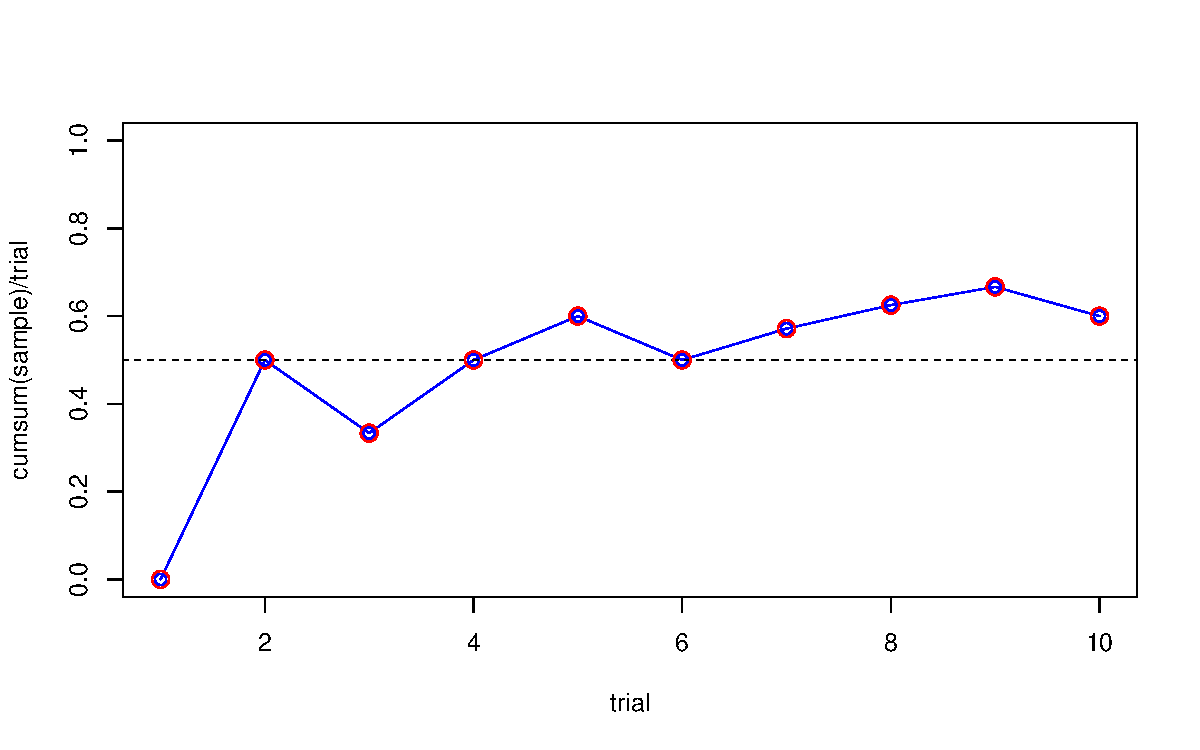
\includegraphics[width=0.72\textwidth]{Section5/images/simulation_plot.pdf}
  \caption{Simulation of running sample mean of Bernoulli(\(p = 0.5\)) trials over time.}
\end{figure}

{\color{gray} \textbf{R Simulation Code (Single Sample Path)}}

\begin{verbatim}
n = 10
trial = seq(1, n, by = 1)
sample = rbinom(n, 1, 1/2)

plot(trial, cumsum(sample)/trial, type = "l", ylim = c(0,1), col = "blue")
points(trial, cumsum(sample)/trial, col = "red")
abline(h = 0.5, lty = 2, col = "black")
\end{verbatim}

\begin{figure}[H]
  \centering
  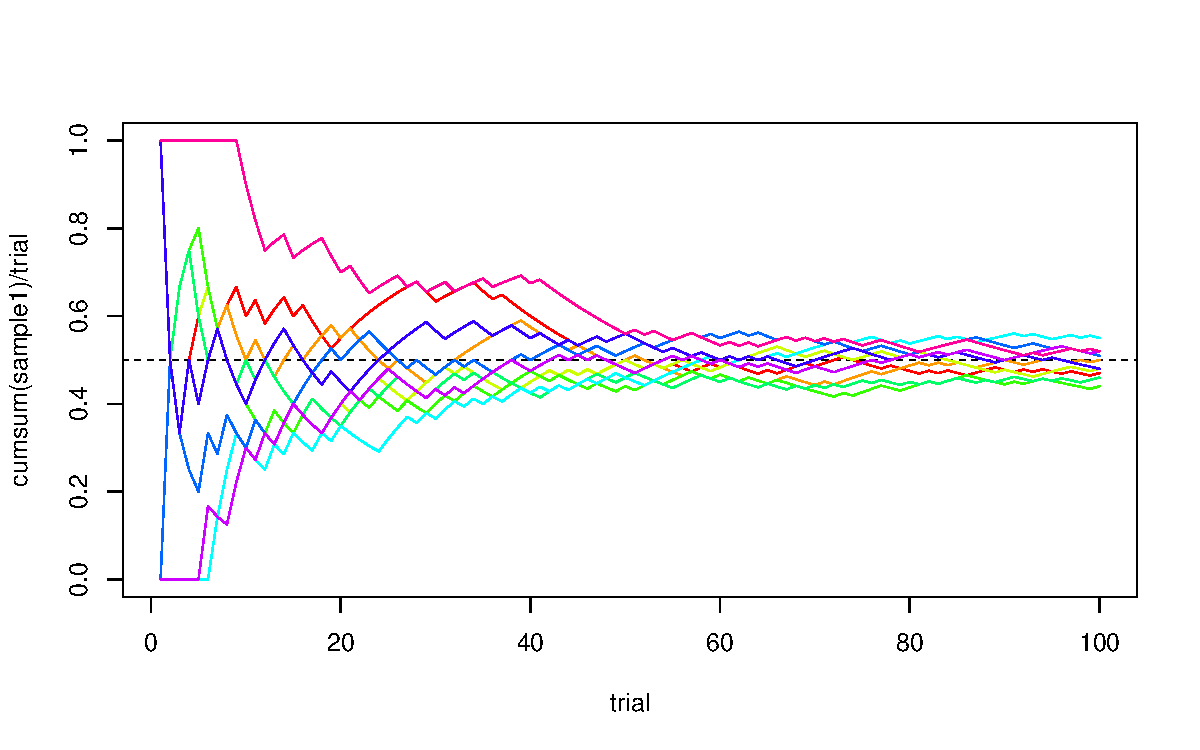
\includegraphics[width=0.72\textwidth]{Section5/images/simulation_multi.pdf}
  \caption{Simulation of 10 running sample means of Bernoulli(\(p = 0.5\)) trials converging over 100 trials.}
\end{figure}


{\color{gray} \textbf{R Simulation Code (Multiple Sample Paths)}}


\begin{verbatim}
n = 100
trial = seq(1, 100, by = 1)

sample1 = rbinom(n, 1, 1/2)
sample2 = rbinom(n, 1, 1/2)
sample3 = rbinom(n, 1, 1/2)
sample4 = rbinom(n, 1, 1/2)
sample5 = rbinom(n, 1, 1/2)
sample6 = rbinom(n, 1, 1/2)
sample7 = rbinom(n, 1, 1/2)
sample8 = rbinom(n, 1, 1/2)

colors = rainbow(8)


plot(trial, cumsum(sample1)/trial, type = "l", col = colors[1], ylim = c(0,1))
lines(trial, cumsum(sample2)/trial, col = colors[2])
lines(trial, cumsum(sample3)/trial, col = colors[3])
lines(trial, cumsum(sample4)/trial, col = colors[4])
lines(trial, cumsum(sample5)/trial, col = colors[5])
lines(trial, cumsum(sample6)/trial, col = colors[6])
lines(trial, cumsum(sample7)/trial, col = colors[7])
lines(trial, cumsum(sample8)/trial, col = colors[8])
abline(h = 0.5, lty = 2, col = "black")
\end{verbatim}


\subsection*{Empirical Probability Insight}


The Law of Large Numbers gives us empirical probabilities. Consider tossing a fair coin. Define the random variable \( X \) as:

\[
X = \begin{cases}
1 & \text{heads up} \\
0 & \text{tails up}
\end{cases}
\]

Then as we sample more and more values of \( X \), the sample mean \( \bar{X}_n \) converges in probability to \( P(\text{heads up}) \), that is:

\[
\bar{X}_n \xrightarrow{P} P(\text{heads up}) 
\]



%\section{Practice Assignment 4} \label{ssec.ass5}\markright{\ref{ssec.ass5}
%\titleref{ssec.ass5}}
%
%\begin{enumerate}
\item For the following question, let
$$ {\bf u}=(1,0,-2,0) \quad {\bf v}=(2,3,4,-1)  \quad {\bf
w}=(4,2,0,-1) \quad {\bf x}=(2,-3,-1,1). $$ Find
\begin{enumerate}
\item (i) ${\bf u}+{\bf v}$ \quad (ii) $2{\bf u}-3{\bf x}+{\bf v}$
\quad (iii) $c$ such that ${\bf x}+{\bf v}+c{\bf w}=(0,-2,3,1)$
\item (i) ${\bf v}\cdot {\bf w}$ \quad (ii) ${\bf x}\cdot {\bf v}$
\quad (iii) ${\bf v}\cdot({\bf x}+{\bf w}) $
\item (i) ${\bf x} \cdot (2{\bf v}-{\bf w})$ \quad (ii)
$({\bf w}\cdot {\bf x}){\bf u}-({\bf u}\cdot {\bf x}){\bf v}$
\item (i) $\| {\bf u} \|$ \quad (ii)$ \|{\bf v} \|$ \quad (iii)$\| 7{\bf x}-6{\bf w}\| $
\item The length of {\bf x}.
\item (i) $\frac{1}{\|{\bf w}\|}{\bf w}$ \quad (ii) $ \| \frac{1}{\|{\bf w}\|}{\bf w}\|$
\item The distance between the endpoints of {\bf v} and {\bf w}
\item The cosine of the angle between {\bf x} and {\bf w}. What
kind of angle is it?
\item The cosine of the angle between {\bf u} and {\bf v}. What
kind of angle is it?
\end{enumerate}
\begin{description}\item  (a) (i)
\begin{eqnarray*}
{\bf u}+{\bf v}&=&(1,0,-2,0)+(2,3,4,-1)
\\&=&(1+2,0+3,-2+4,0+(-1))
\\&=&(3,3,2,-1)
\end{eqnarray*}
\item\quad\, (ii)
\begin{eqnarray*}
2{\bf u}-3{\bf x}+{\bf v}&=&2(1,0,-2,0)-3(2,-3,-1,1)+(2,3,4,-1)
\\&=&(2,0,-4,0)+(-6,9,3,-3)+(2,3,4,-1)
\\&=&(-2,12,3,-4)
\end{eqnarray*}
\item \quad\, (iii)
\begin{eqnarray*}
&&{\bf x}+{\bf v}+c{\bf w}=(0,-2,3,1)
\\&&(2,-3,-1,1)+(2,3,4,-1)+c(4,2,0,-1)=(0,-2,3,1)
\\&&(4+4c,2c,3,-c)=(0,-2,3,1)
\\&&c=-1 satisfies this condition.
\end{eqnarray*}
\item (b) (i)
\begin{eqnarray*}
{\bf v}\cdot{\bf w}&=&(2,3,4,-1) \cdot (4,2,0,-1)
\\&=&(2)(4)+(3)(2)+(4)(0)+(-1)(-1)
\\&=&15
\end{eqnarray*}
\item\quad\, (ii)
\begin{eqnarray*}
{\bf x} \cdot {\bf v}&=&(2,-3,-1,1) \cdot (2,3,4,-1)
\\&=&4-9-4-1
\\&=&-10
\end{eqnarray*}
\item\quad\, (iii)
\begin{eqnarray*}
{\bf v} \cdot ({\bf x} + {\bf w})&=&(2,3,4,-1) \cdot \left[(2,-3,-1,1)+(4,2,0,-1)\right]
\\&=&(2,3,4,-1) \cdot (6,-1,-1,0)
\\&=&12-3-4+0
\\&=&5
\end{eqnarray*}
\item (c) (i)
\begin{eqnarray*}
{\bf x}\cdot(2{\bf v}-{\bf w})
&=&(2,-3,-1,1) \cdot \left[2(2,3,4,-1)-(4,2,0,-1) \right]
\\&=&(2,-3,-1,1) \cdot (0,4,8,-1)
\\&=&0-12-8-1
\\&=&-21
\end{eqnarray*}
\item\quad\, (ii)
\begin{eqnarray*}
({\bf w} \cdot {\bf x}){\bf u}-({\bf u} \cdot {\bf x}){\bf v}
&=&\left[(4,2,0,-1) \cdot (2,-3,-1,1)\right](1,0,-2,0)
\\&&-\left[(1,0,-2,0) \cdot (2,-3,-1,1)
\right](2,3,4,-1)
\\
&=&(1)(1,0,-2,0)-(4)(2,3,4,-1)
\\
&=&(1,0,-2,0)+(-8,-12,-16,4)
\\
&=&(-7,-12,-18,4)
\end{eqnarray*}
\item (d) (i)
\begin{eqnarray*}
\| {\bf u} \|&=&\sqrt{(1)^{2}+(0)^{2}+(-2)^{2}+(0)^{2}}
\\&=&\sqrt{1+0+4+0}
\\&=&\sqrt{5}
\end{eqnarray*}
\item\quad\, (ii)
\begin{eqnarray*}
\| {\bf v} \|&=&\sqrt{(2)^{2}+(3)^{2}+(4)^{2}+(-1)^{2}}
\\&=&\sqrt{4+9+16+1}
\\&=&\sqrt{30}
\end{eqnarray*}
\item\quad\, (iii)
\begin{eqnarray*}
\| 7{\bf x}-6{\bf w} \|&=&\| 7(2,-3,-1,1)-6(4,2,0,-1) \|
\\&=&\|(-10,-33,-7,13)\|
\\&=&\sqrt{(-10)^{2}+(-33)^{2}+(-7)^{2}+(13)^{2}}
\\&=&\sqrt{1407}
\end{eqnarray*}
\item (e) The length of ${\bf x}=\|{\bf x}\|=\sqrt{15}$\\
\item (f) (i) First, $\|{\bf w}\|=\sqrt{21}$. So:
$\frac{1}{\|{\bf w}\|}{\bf
w}=(\frac{4}{\sqrt{21}},\frac{2}{\sqrt{21}},0,-\frac{1}{\sqrt{21}})$
\item\quad\, (ii)
\begin{eqnarray*}
\|\frac{1}{\|{\bf w}\|}{\bf w}\|&=&\sqrt{(\frac{4}{\sqrt{21}})^2+(\frac{2}{\sqrt{21}})^2,0,(-\frac{1}{\sqrt{21}})^2}
\\&=&\sqrt{\frac{21}{21}}
\\&=&1
\end{eqnarray*}
\item (g)
The distance between the endpoints of {\bf v} and {\bf
w} is d$({\bf v},{\bf w})$.
\begin{eqnarray*} d({\bf v},{\bf w})
&=&\|{\bf v}-{\bf w}\|
\\&=&\sqrt{(2-4)^2+(3-2)^2+(4-0)^2+(-1+1)^2}
\\&=&\sqrt{21}
\end{eqnarray*}
\item (h)
\begin{eqnarray*}
&&\cos\theta=\frac{ {\bf x} \cdot {\bf w} }{ \|{\bf x}\|  \|{\bf
w}\|}
\\&&\cos\theta=\frac{1}{(\sqrt{15})(\sqrt{21})}
\\&&\cos\theta=\frac{1}{\sqrt{315}}
\end{eqnarray*}
The angle is acute ($\theta \doteq 86.8$ degrees).
\item (i) \begin{eqnarray*}&&\cos\theta=\frac{ {\bf u} \cdot {\bf v} }{ \|{\bf u}\|  \|{\bf
v}\| }
\\&&\cos\theta=\frac{-6}{(\sqrt{5})(\sqrt{30})}
\\&&\cos\theta=\frac{-6}{\sqrt{150}}
\end{eqnarray*}
\noindent The angle is obtuse ($\theta \doteq 119.3$ degrees).
\end{description}

\item Find a vector, $(a,b,c,d)$, that is orthogonal to
$(-1,0,0,1)$.

\noindent \textbf{Solution}

\noindent If $(a,b,c,d)$ is perpendicular to $(-1,0,0,1)$ then the
dot product of the two vectors is zero.

$(a,b,c,d) \cdot (-1,0,0,1)=0$

$\Rightarrow\ -a+d=0$

\noindent There are many solutions to $-a+d=0$. An example of one
particular vector orthogonal to $(-1,0,0,1)$ is $(1,0,1,1)$.

\item Determine which of the following operations are possible. If
they are not possible, explain why.

(a) $({\bf u} \cdot {\bf x}) \| {\bf w} \| \quad \quad$ (b) $\|
({\bf u} , {\bf v}) \|^2 \quad \quad$ (c) $({\bf u} \cdot {\bf
v},{\bf v} \cdot {\bf w})$

\noindent \textbf{Solution} \begin{description} \item (a)
The operation is possible (scalar times a scalar).
\item (b)
The operation is not possible.  The norm is not defined
for a scalar; it is used to find vector lengths only.
\item (c)
The operation is possible (vectors have scalar components).
\end{description}
\item
\begin{enumerate}
\item If ${\bf v}$ is any 3-tuple, show that $\frac{1}{\bf \|v\|}{\bf
v}$ is a unit vector. What is the direction of this unit vector?
Show that this is true if {\bf v} is any $n$-tuple.
\item For each vector {\bf u} given, find a vector of unit length in the
same direction as {\bf u}.

(i) ${\bf u}=(-1,4)$ \quad \quad \quad\quad\,\,\,(ii) ${\bf u}=(-6,1,-5,-3)$ \quad
\quad

(iii) ${\bf u}=(1,1,1,-1)$ \quad \quad (iv) ${\bf
u}=(1,5,0,-1,-7)$
\end{enumerate}

\noindent \textbf{Solution} \begin{description} \item (a)
Let ${\bf v}$ be any 3-tuple such that:

${\bf v}=(a,b,c)$ \quad \quad $a,b,c\in$ {\tebbb R}

\noindent $\|{\bf v}\|=\sqrt{a^{2}+b^{2}+c^{2}}$
\begin{eqnarray*}
\frac{1}{\|{\bf v}\|}{\bf v}=
(\frac{a}{\sqrt{a^{2}+b^{2}+c^{2}}},\frac{b}{\sqrt{a^{2}+b^{2}+c^{2}}},
\frac{c}{\sqrt{a^{2}+b^{2}+c^{2}}})
\end{eqnarray*}
\noindent We know that $\frac{1}{\|{\bf v}\|}{\bf v}$ is a unit
vector because the norm of the vector is $1$. Examine:
\begin{eqnarray*} \|\frac{1}{\|{\bf v}\|}{\bf v}\|
&=&\sqrt{  (\frac{a}{\sqrt{a^{2}+b^{2}+c^{2}}})^{2} +
(\frac{b}{\sqrt{a^{2}+b^{2}+c^{2}}})^{2} +
(\frac{c}{\sqrt{a^{2}+b^{2}+c^{2}}})^{2} }
\\&=&\sqrt{ \frac{a^{2}}{\sqrt{a^{2}+b^{2}+c^{2}}}  +
\frac{b^{2}}{\sqrt{a^{2}+b^{2}+c^{2}}} +
\frac{c^{2}}{\sqrt{a^{2}+b^{2}+c^{2}}} }
\\&=&\sqrt{\frac{a^{2}+b^{2}+c^{2}}{a^{2}+b^{2}+c^{2}} }
\\&=&\sqrt{1}=1
\end{eqnarray*}

\noindent The vector $\frac{1}{\|{\bf v}\|}{\bf v}$ points in the
same direction as the original ${\bf b}$ vector.

\noindent This is true if ${\bf v}$ is any n-tuple vector.
Examine:

${\bf v}=(x_{1},x_{2},....,x_{n})$ where
$x_{1},x_{2},...,x_{n}\in$ {\tebbb R}
\begin{eqnarray*}
\|{\bf v} \|= \sqrt{x_{1}^{2}+x_{2}^{2}+.....+x_{n}^{2}}
\end{eqnarray*}
$\frac{1}{\|{\bf v} \|}{\bf
v}=(\frac{x_{1}}{\sqrt{x_{1}^{2}+x_{2}^{2}+.....+x_{n}^{2}}},\frac{x_{2}}{\sqrt{x_{1}^{2}
+x_{2}^{2}+.....+x_{n}^{2}}},...,\frac{x_{n}}{\sqrt{x_{1}^{2}+x_{2}^{2}+.....+x_{n}^{2}}})$

\begin{enumerate} \item[$\|\frac{1}{\|{\bf v} \|}{\bf v} \|$]

$=\sqrt{(\frac{x_{1}}{
\sqrt{x_{1}^{2}+x_{2}^{2}+.....+x_{n}^{2}}})^{2}+(\frac{x_{2}}{
\sqrt{x_{1}^{2}+x_{2}^{2}+.....+x_{n}^{2}}})^{2}+...+(\frac{x_{n}}{
\sqrt{x_{1}^{2}+x_{2}^{2}+.....+x_{n}^{2}}})^{2}}$

$=\sqrt{\frac{x_{1}^{2}}{x_{1}^{2}+x_{2}^{2}+.....+x_{n}^{2}}
+\frac{x_{2}^{2}}{x_{1}^{2}+x_{2}^{2}+.....+x_{n}^{2}}+...+\frac{x_{n}^{2}}{x_{1}^{2}+x_{2}^{2}
+.....+x_{n}^{2}}}$

$=\sqrt{\frac{ x_{1}^{2}+x_{2}^{2}+...+x_{n}^{2} }
{x_{1}^{2}+x_{2}^{2}+...+x_{n}^{2} }  }$

$=\sqrt{1}=1$

\end{enumerate}

\item (b) (i)
${\bf u}=(-1,4)$

$\|{\bf u}\|=\sqrt{17}$

$\frac{1}{\|{\bf u}\|}{\bf
u}=(-\frac{1}{\sqrt{17}},\frac{4}{\sqrt{17}})$ is a vector of unit
length in the same direction as ${\bf u}$.
\item\quad\, (ii)
${\bf u}=(-6,1,-5,-3)$

$\|{\bf u}\|=\sqrt{71}$

$\frac{1}{\|{\bf u}\|}{\bf
u}=(-\frac{6}{\sqrt{71}},\frac{1}{\sqrt{71}},-\frac{5}{\sqrt{71}},-\frac{3}{\sqrt{71}}
)$ is a vector of unit length in the same direction as ${\bf u}$.
\item\quad\, (iii)
${\bf u}=(1,1,1,-1)$
$\|{\bf u}\|=\sqrt{4}$
$\frac{1}{\|{\bf u}\|}{\bf
u}=(\frac{1}{\sqrt{4}},\frac{1}{\sqrt{4}},\frac{1}{\sqrt{4}},-\frac{1}{\sqrt{4}}
)$ is a vector of unit length in the same direction as ${\bf u}$.
\item \quad\, (iv)
${\bf u}=(1,5,0,-1,-7)$
$\|{\bf u}\|=\sqrt{76}$
$\frac{1}{\|{\bf u}\|}{\bf
u}=(\frac{1}{\sqrt{76}},\frac{5}{\sqrt{76}},0,-\frac{1}{\sqrt{76}},-\frac{7}{\sqrt{76}})$
is a vector of unit length in the same direction as ${\bf u}$.
\end{description}

\item Determine $t$ so that the following vectors are of unit
length in $\mbox{\tebbb R}^4$, if possible.

(a) $(t,-\frac{1}{4},\sqrt{2},0) \quad \quad$ (b)
$(\frac{t}{2},0,-\frac{t}{6}, -t)$

\noindent \textbf{Solution} \begin{description} \item (a)
If $(t,-\frac{1}{4},\sqrt{2},0) \cdot
(t,-\frac{1}{4},\sqrt{2},0)=1$ then $(t,-\frac{1}{4},\sqrt{2},0)$
is of unit length. Thus

$t^2+(-\frac{1}{4})^2+(\sqrt{2})^2+0=1\ \Rightarrow\
t^2=-\frac{{17}}{16}$

\noindent There is no real root that will satisfy this condition;
thus, $(t,-\frac{1}{4},\sqrt{2},0)$ cannot be of unit length.
\item (b)
If $(\frac{t}{2},0,-\frac{t}{6}, -t)\cdot
(\frac{t}{2},0,-\frac{t}{6}, -t)=1$ then
$(\frac{t}{2},0,-\frac{t}{6}, -t)$ is of unit length. Thus:
$( \frac{t}{2}  )^{2}+( -\frac{t}{6}  )^{2}+( -t )^{2}=1\
\Rightarrow\ t=\pm\frac{6}{\sqrt{46}}$
\noindent Thus the vector is of unit length when
$t=\pm\frac{6}{\sqrt{46}}$.
\end{description}

\item \begin{enumerate}
\item For ${\bf u}=(4,1,0,-a)$ and ${\bf v}=(a,2,-1,-5a)$,
find $a$ so that ${\bf u} \cdot {\bf v}=0$.
\item For ${\bf u}=(a,3,-2,5)$, find $a$ so that $\|{\bf u}\|=9$.
\end{enumerate}

\noindent \textbf{Solution} \begin{description} \item (a)
${\bf u} \cdot {\bf v}=0$

$(4,1,0,-a) \cdot (a,2,-1,-5a)=0$

$4a+2+0+5a^2=0$

So $a=\frac{-2\pm \sqrt{6}i}{5}$ when ${\bf u} \cdot {\bf v} =0$,
where $i^2 = -1$ .
\item (b)
$\|{\bf u}\|=9$

$\Rightarrow \sqrt{(a)^{2}+(3)^{2}+(-2)^{2}+(5)^{2}}=9$

$(a^{2}+38)^{\frac{1}{2}}=9$

$a^{2}+38=81$

$a=\pm\sqrt{43}$

\noindent Then $a=\pm\sqrt{43}$ when $\|{\bf u}\|=9$.
\end{description}

\item Let ${\bf{u}} = (1, 2, 3, 4)$ and ${\bf{v}} = (-1, 0, 1, 1)$. Find
\begin{enumerate}
\item the vector projection of ${\bf{u}}$ on ${\bf{v}}$
\item the vector projection of ${\bf{v}}$ on ${\bf{u}}$
\item use your answer to (a) to find a vector orthogonal to ${\bf{v}}$
\end{enumerate}

\noindent \textbf{Solution} \begin{description} \item (a) Projection of ${\bf{u}}$ on ${\bf{v}}$
\begin{eqnarray*}
&=&\frac{{\bf{u}} \cdot {\bf{v}}}{{\bf{v}}\cdot{\bf{v}}}\,{\bf{v}} \\&=& \frac{-1 + 3 + 4}{-1^2 + 1^2 + 1^2}\,(-1,0,1,1)\\
&=&2(-1, 0, 1, 1) \\&=& (-2, 0, 2, 2)
\end{eqnarray*}
\item (b) Projection of ${\bf{v}}$ on ${\bf{u}}$
\begin{eqnarray*}
&=&\frac{{\bf{v}} \cdot {\bf{u}}}{{\bf{u}}\cdot{\bf{u}}}\,{\bf{u}} \\&=& \frac{6}{1^2 + 2^2 + 3^2 + 4^2}\,(1,2,3,4)\\
&=&\tfrac{1}{5}(1, 2, 3, 4)
\\&=& (\tfrac{1}{5}, \tfrac{2}{5}, \tfrac{3}{5}, \tfrac{4}{5})
\end{eqnarray*}
\item (c) ${\bf{u}}$ - (projection of ${\bf{u}}$ on ${\bf{v}}$) is orthogonal to ${\bf{v}}$
\begin{equation*}
(1,2,3,4) - (-2,0,2,2) = (3,2,1,2)
\end{equation*}
\end{description}

\item Find the equation of the plane through $(-1,2,-3)$ with normal vector $(8,1,1)$.\\

\noindent \textbf{Solution}

Plane through $(x_0, y_0, z_0)$ with normal $(a, b, c)$ has equation
$$
ax + by + cz = ax_0 + by_0 + cz_0.
$$
Required equation is
$$
8x + y + z = -8 + 2 -3,\ \mathrm{i.e.}\ 8x+y+z = -9
$$

\item
\begin{enumerate}
\item For what values of $r$ do the points $(1,2,r),\ (-2,r,3),\ (2,0,-1),\ (0,1,1)$ lie on the same plane?
\item What is the equation of the plane in this case?
\end{enumerate}

\noindent \textbf{Solution} 

\begin{description} \item (a) The equation of the plane through $(1,2,r),\ (2,0,-1),\ (0,1,1)$ is
\begin{align*}
\left| \begin{array}{rrrr} x & y & z & -1 \\ 1 & 2 & r & -1 \\ 2 & 0 & -1 & -1 \\ 0 & 1 & 1 & -1 \end{array} \right|&
= \left| \begin{array}{cccc} x & y-1 & z-1 & 0 \\ 1 & 1 & r-1 & 0 \\ 2 & -1 & -2 & 0 \\ 0 & 1 & 1 & -1 \end{array} \right| \\
&= - \left| \begin{array}{ccc} x & y-1 & z-1 \\ 1 & 1 & r-1 \\ 2 & -1 & -2 \end{array} \right| \\
&= -\bigl\{x(-2+r-1) - (y-1)(-2-2r+2)\\&\quad \quad +(z-1)(-1-2)\bigr\} \\
&= -\bigl\{ (r-3)x + 2ry - 3z - 2r+3 \bigr\} = 0, \\ & \mathrm{i.e.}\ (r-3)x + 2ry-3z = 2r-3.
\end{align*}
$(-2, r, 3)$ lies on this plane if
\begin{align*}
(r-3)(-2) + 2r\cdot r -3 \cdot 3 &= 2r-3 \\
2r^2 - 4r &= 0, \quad r= 0,2.
\end{align*}
\item (b) When $r=0$, the equation is
\begin{align*}
-3x -3z = -3, \quad \mathrm{or}\ x+z = 1.
\end{align*}
When $r=2$, the equation is
\begin{align*}
-x + 4y -3z = 1, \quad \mathrm{or}\ x-4y+3z=-1.
\end{align*}
\end{description}
\item
\begin{enumerate}
\item For what values of $r$ do the points $(1,1),\,(1,0),\,(-2,1),\,(r,2)$ lie on the same circle?
\item Find the radius of the circle and the coordinates of the center.
\end{enumerate}
\smallskip

\noindent \textbf{Solution} \begin{description} \item (a) The equation of the circle through $(1,1),\,(1,0),\,(-2,1)$ is
\begin{align*}
\left| \begin{array}{cccc} x^2 + y^2 & x & y & 1 \\ 2 & 1 & 1 & 1 \\ 5 & -2 & 1 & 1 \\ 1 & 1 & 0 & 1 \end{array} \right|
&= \left| \begin{array}{cccc} x^2 + y^2-1 & x-1 & y & 0 \\ 1 & 0 & 1 & 0 \\ 4 & -3 & 1 & 0 \\ 1 & 1 & 0 & 1 \end{array} \right| \\
&=  \left| \begin{array}{ccc} x^2 + y^2-1 & x-1 & y \\ 1 & 0 & 1 \\ 4 & -3 & 1 \end{array} \right|\\
&= (x^2 + y^2-1)\cdot 3 - (x-1)(-3) + y(-3)\\
&= 3(x^2 + y^2) + 3x - 3y -6 = 0, \\& \mathrm{i.e.}\ x^2 + y^2 + x-y = 2
\end{align*}
$(r,2)$ lies on this circle if
$$
r^2+4+r-2=2,\quad \mathrm{i.e.}\ r=0,-1.
$$
\item (b) Complete the squares:
$$
x^2 + x + \tfrac{1}{4} + y^2 - y + \tfrac{1}{4} = 2 + \tfrac{1}{4} \cdot \tfrac{1}{4} \quad \mathrm{i.e.}\ (x+\tfrac{1}{2})^2 + (y-\tfrac{1}{2})^2 = \tfrac{5}{2}.
$$
The coordinates of the center of the circle are $(-\tfrac{1}{2},\tfrac{1}{2})$ and the radius is $\sqrt{\tfrac{5}{2}}$.
\end{description}
\item If $(-2,3,r)$ lies on the plane through $(-3, 4, 2)$ with normal $(1, r, -1)$, find the value of $r$ and the equation of the plane.

\noindent \textbf{Solution}

The plane through $(-3, 4, 2)$ with normal $(1, r, -1)$ has equation
$$
x + ry - z = -3 + 4r -2 = 4r -5.
$$
$(-2,3,r)$ lies on the plane if
$$
-2 + r \cdot 3 - r = 4r -5, \quad \mathrm{i.e.}\ 3 = 2r,\ r= \tfrac{3}{2}
$$
The equation of the plane is
$$
x + \tfrac{3}{2}y -z = 1, \quad \mathrm{i.e.}\ 2x + 3y - 2z = 2.
$$
\item A parabola with certain orientation has equation
$ay^2+bx+cy+d=0$.  Find the equation of the parabola through the
points $(5,3),(0,-1),(2,1)$.

\noindent \textbf{Solution}

The system of equations
$$ay^2+bx+cy+d=0$$
$$9a+5b+3c+d=0$$
$$a+0b-c+d=0$$
$$a+2b+c+d=0$$ has a non-zero solution.  Therefore
$$\left| \begin{array}{cccc} y^2&x&y&1\\
9&5&3&1\\
1&0&-1&1\\
1&2&1&1\end{array} \right|=0.$$ Evaluating this determinant as in
section \ref{ssec.Danal}, we obtain
$$y^2+8y-8x+7=0.$$
\end{enumerate}


%
%\setcounter{equation}{0}

\chapter{Vector Spaces}
\label{sec.vspace} \pagestyle{myheadings}
\markboth{\ref{sec.vspace}. \titleref{sec.vspace}}{}

Up to now, we have described vectors as $n-$tuples in
$\mbox{\tebbb R}^n$. They have been presented geometrically as
arrows in 2 and 3-space. In this section we view vectors in a
broader perspective. Ten axioms are presented. Any set that
satisfies these axioms will be called a vector space and the
elements in the set are called vectors. We will learn to identify
subspaces of a vector space, to write vectors as a linear
combination of one another and to construct a basis for a vector
space. Every vector in the vector space can be written as a linear
combination of the basis vectors.

\noindent {\bf Learning Objectives}
\index{linear combination}
\begin{itemize}
\item determine whether or not a set is a subspace of a vector space
\item express vectors as linear combinations of other vectors
\item determine whether a set of vectors is linearly independent
or linearly dependent
\item determine whether a set of vectors spans a vector space
\item determine whether a set of vectors is a basis for a vector
space
\item find the dimension of a vector space
\item find the coordinates of a vector with respect to a basis
\end{itemize}

\section{Definition of a Vector Space} \label{ssec.defvs}\markright{\ref{ssec.defvs} \titleref{ssec.defvs}}
\index{vector space}\index{basis}
Let $V$ be any non-empty set of objects on which two operations
are defined: ${\bf u}+{\bf v}$ and $k{\bf v}$.  If the following
axioms are met by all objects {\bf u,v} and {\bf w} in $V$, for
all scalars $k$ and $l$, then $V$ is called a {\bf vector space},
and the objects in $V$ are called {\bf vectors}.
\begin{enumerate}
\item For all ${\bf u, v}$ in $ V$, the sum ${\bf u}+{\bf v}$ is also in $V$ .
\item ${\bf u}+{\bf v}={\bf v}+{\bf u}$.
\item ${\bf u}+({\bf v}+{\bf w})=({\bf u}+{\bf v})+{\bf w}$.
\item There exists a zero element, ${\bf 0}$ in $V$, such that ${\bf 0+v}={\bf
v+0}={\bf v}$.
\item For all ${\bf u}$ in $V$, there exists a ${\bf -u}$ in $V$, such that
${\bf u +(-u)}={\bf (-u)+u}={\bf 0}$.
\item For all ${\bf u}$ in $V$, the product $k{\bf u}$ is also in $V$.
\item $k({\bf u}+{\bf v})=k{\bf u}+k{\bf v}$.
\item $(k+l){\bf u}=k{\bf u}+l{\bf u}$.
\item $k(l{\bf u})=(kl){\bf u}$.
\item $1{\bf u}={\bf u}$.
\end{enumerate}

A vector space need not be composed of the vectors introduced in
the previous sections.  A vector space is any set of elements that
satisfies the above ten axioms.  The elements in that set are called vectors.
Thus, a vector can be
a matrix or even a function. Similarly, although the operations of
a vector space are given as ``addition" and ``scalar
multiplication", they need not be defined in the usual sense of
addition and scalar multiplication. The only requirement is that
the ten vector space axioms be met.

In this course we will consider primarily the vector spaces
$\mbox{\tebbb R}^n$ $(n\geq1)$. It is not intended that you
memorize the ten axioms above. The axioms do no more than dictate
that vector addition and scalar multiplication behave in a
sensible way.

\section{Subspaces}
\label{ssec.subspace}\markright{\ref{ssec.subspace}
\titleref{ssec.subspace}}
\index{subspace}
A subset $W$ of a vector space $V$ is a {\bf subspace} of $V$ if
it is also a vector space under the addition and scalar
multiplication of $V$.

In the case of a subspace, it is not necessary to show that all
ten axioms are satisfied. If $W$ is a subset of $V$, most of
axioms will hold for $W$ because they hold for $V$. In fact, $W$
is a subspace of $V$ if and only if the following conditions are
met.

\begin{enumerate}
\item  $W$ is non-empty.
\item For all ${\bf u,v}$ in $W$,  ${\bf u}+{\bf v}$ is in $W$ (closed
under addition). \item For all $ k$ in $\mbox{\tebbb R}$ and for
all ${\bf u}$ in $W$, $k{\bf u}$ is in $W$ (closed under scalar
multiplication).
\end{enumerate}

Since every vector space has to have a zero vector, an easy way to
show that $W$ is non-empty is to show that ${\bf 0}~\in~W$.

\subsection*{Examples of Subspaces}

The following is a list of the subspaces of $\mbox{\tebbb R}^2$
and $\mbox{\tebbb R}^3$. Verification is left as an exercise.

\begin{enumerate}
\item Subspaces of $\mbox{\tebbb R}^2$:
\begin{itemize}
\item \{{\bf 0}\}=\{(0,0)\}, the set consisting of the zero vector alone.
This subspace consists of a single point: the origin.
\item Lines through the origin.  If ($x_0,y_0$) is a non-zero
vector in $\mbox{\tebbb R}^2$ then the set \{$c(x_0,y_0)$:$c$ $\in$ $\mbox{\tebbb R}$\},
the set of all multiples of ($x_0,y_0$), is the line through the origin and ($x_0,y_0$).
\item $\mbox{\tebbb R}^2$.  We can think of  $\mbox{\tebbb R}^2$ as a subset of itself,
and so viewed it is a vector subspace.  The subspaces \{{\bf 0}\} and $\mbox{\tebbb R}^2$
are called improper subspaces.\\
\end{itemize}
\item Subspaces of $\mbox{\tebbb R}^3$
\begin{itemize}
\item \{{\bf 0}\}=\{(0,0,0)\}, the set consisting of the zero vector alone.
This subspace consists of a single point: the origin.
\item Lines through the origin.  If ($x_0,y_0,z_0$) is a non-zero
vector in $\mbox{\tebbb R}^3$ then the set \{$c(x_0,y_0,z_0)$: $c$ $\in$ $\mbox{\tebbb R}$\},
the set of all multiples of ($x_0,y_0,z_0$), is the line through the origin and ($x_0,y_0,z_0$).
\item Planes through the origin.  If ($x_0,y_0,z_0$), ($x_1,y_1,z_1$) are non-zero points in
$\mbox{\tebbb R}^3$, not on the same straight line through the origin
(so neither is a multiple of the other),
then \{$c_0(x_0,y_0,z_0)+c_1(x_1,y_1,z_1)$: $c_0, c_1$ $\in$ $\mbox{\tebbb R}$\} is a plane
through the origin.  To evaluate the expression $c_0(x_0,y_0,z_0)+c_1(x_1,y_1,z_1)$, we extend
the vectors $(x_0,y_0,z_0)$, $(x_1,y_1,z_1)$ by factors $c_0$, $c_1$ respectively and then add
using the parallelogram law.  By varying $c_0$ and $c_1$ (remember $c_0$, $c_1$ can be negative
as well as positive) we obtain all the points in the plane through the origin $(x_0,y_0,z_0)$ and $(x_1,y_1,z_1)$.
\item $\mbox{\tebbb R}^3$.  We can think of $\mbox{\tebbb R}^3$ as a subset
of itself, and then it is a vector subspace of itself.  The subspaces \{{\bf 0}\} and $\mbox{\tebbb R}^3$ are called improper subspaces.
\end{itemize}
\item The solution set of the homogeneous linear system $A{\bf
x}={\bf 0}$ with $m$ equations and $n$ unknowns, is a subspace of
$\mbox{\tebbb R}^n$.  This set is called the solution space of the
system.
\end{enumerate}

\begin{example}
\label{exam5.subspaces1}

\noindent Let $W=\{(x,y,z): x,y,z \in ${\tebbb R} and $
x^2+y^2+z^2 \leq 1 \}$. Is $W$ a subspace of {\tebbb R}$^{3}$? Why
or why not?

To prove that $W$ is a subspace of {\tebbb R}$^{3}$ we must show
that it is non-empty,

closed under addition and closed under scalar multiplication.

Is $W$ closed under scalar multiplication?

Note that for example, $(0,1,0)~\in~W$ because $0^2+1^2+0^2=1$. However

$2(0,1,0)=$ $(0,2,0)$ does not belong to $W$ because $0^2+2^2+0^2=4$. Thus $W$

is not closed under scalar multiplication. $W$ is therefore not a subspace.

As a matter of fact, $W$ is not closed under addition either. Examine

two vectors in $W$, ${\bf v}=(1,0,0)\ \ and\ \ {\bf u}=(0,0,1)$. The sum of these

vectors is: $${\bf v}+ {\bf u}= (1,0,0)+(0,0,1)=(1,0,1)$$

but $(1,0,1)$ is not in $W$ because $1^2+0^2+1^2=1+0+1=2$ which is
not

less than or equal to 1.

\end{example}

\noindent {\bf Activity \ref{ssec.subspace}:}

\begin{enumerate}
\item Verify that vectors on a line through the origin make up a
subspace of $\mbox{\tebbb R}^2$. Why is it important that the line
pass through the origin?
\item The solution set of $A{\bf x}={\bf 0}$ consists of vectors
of the form ${\bf x}=\left [ \begin{array}{c} x_1\\x_2\\ \vdots\\
x_n \end{array} \right ]$.  Show that the set of
solutions is a subspace by verifying the three axioms. Why isn't
the set of solutions to $A{\bf x}={\bf b}$ a subspace when ${\bf
b}\neq {\bf 0}$?
\end{enumerate}

\noindent Hints are given in the section \ref{answers5}.

\section{Linear Combinations of Vectors}\index{linear combination of vectors}
\label{ssec.lincomb}\markright{\ref{ssec.lincomb}
\titleref{ssec.lincomb}}

In this section, we introduce the idea of writing one vector as
the sum of other vectors.

The vector {\bf w} is a {\bf linear combination} of the vectors
${\bf v}_1,{\bf v}_2, \ldots ,{\bf v}_r$ if it can be expressed as
follows: $${\bf w}=k_1{\bf v}_1+k_2{\bf v}_2+ \cdots + k_r{\bf
v}_r$$ where $k_i \in \mbox{\tebbb R}$.

\begin{example}
\label{exam5.standvec}

The standard unit vectors for $\mbox{\tebbb R}^3$, are {\bf
i}=$(1,0,0)$, {\bf j}=$(0,1,0)$ and {\bf k}=$(0,0,1)$.  All
vectors of the form ${\bf v}=(v_1,v_2,v_3)$ can be written as a
linear combination of the standard unit vectors. $${\bf v}=v_1{\bf
i}+v_2{\bf j}+v_3{\bf k}=v_1(1,0,0)+v_2(0,1,0)+v_3(0,0,1).$$
\end{example}

By expressing linear combinations, we are essentially referencing
a vector with respect to other known vectors.  The previous
example demonstrated this by using the standard unit vectors as
these references.  This is similar to the coordinate axes of the
Cartesian coordinate system.  When we express vectors in terms of
the coordinate system, we are expressing them with respect to the
mutually perpendicular $x,y$ and $z$ axes.

The vectors we use as reference points need not be perpendicular
to each other.  The following example shows how to express a
vector with respect to other vectors which are not necessarily
standard unit vectors.

\begin{example}
\label{exam5.lincomb} Let ${\bf u}=(-1,3,2)$ and ${\bf
v}=(6,-7,1)$.  Show that ${\bf w}=(-9,16,5)$ is a linear
combination of {\bf u} and {\bf v}.

We need to find $k_1$ and $k_2$ such that
\begin{eqnarray*}
{\bf w}&=&k_1{\bf u}+k_2{\bf v}\\
(-9,16,5)&=&k_1(-1,3,2)+k_2(6,-7,1)\\
\\ &\Rightarrow& \left \{ \begin{array}{l}
                            -9=-k_1+6k_2\\
                            16=3k_1-7k_2 \quad \quad .  \\
                            5=2k_1+k_2\end{array} \right .
\end{eqnarray*}
The augmented matrix of this system is $$\left[
\begin{array}{rrcr}-1&6&\vline&-9 \\ 3&-7&\vline&16 \\
2&1&\vline&5 \end{array} \right]~which~reduces~to~\left[
\begin{array}{rrcr}1&0&\vline&3 \\ 0&1&\vline&-1 \\
0&0&\vline&0 \end{array} \right].$$ This means that the system is
consistent and $k_1=3$, $k_2=-1$.

\noindent Therefore {\bf w} is a linear combination of {\bf u} and
{\bf v}: $$(-9,16,5)=3(-1,3,2)-(6,-7,1).$$
\end{example}
\begin{example}
\label{exam5.lincomb2}
Let ${\bf u}=(1,2,-1)$ and ${\bf v}=(0,1,3)$.  Write ${\bf w}=(-1,1,-2)$ as
a linear combination of {\bf u} and {\bf v}.

We must find $k_1, k_2$ such that
${\bf w}=k_1{\bf u}+k_2{\bf v}$,
$$i.e. (-1,1,-2)=k_1(1,2,-1)+k_2(0,1,3),$$
or
$$ 1k_1+0k_2=-1$$
$$2k_1+1k_2=1$$
$$-1k_1+3k_2=-2.$$
The augmented matrix of the system is
$$\left[\begin{array}{rrcr} 1&0&\vline&-1\\
2&1&\vline&1\\
-1&3&\vline&-2\end{array}\right]~which~reduces~to~\left[
\begin{array}{rrcr}1&0&\vline&-1 \\ 0&1&\vline&3 \\
0&0&\vline&-12 \end{array} \right].$$
The system is inconsistent, so {\bf w} cannot be written as a linear combination of
{\bf u} and {\bf v}.
\end{example}

\noindent {\bf Activity \ref{ssec.lincomb}:}

Express the vectors $(1,0,0)$, $(0,1,0)$ and $(0,0,1)$ as linear
combinations of the vectors $(1,2,0)$, $(1,3,4)$, and $(0,-1,4)$.
Answers can be found in section \ref{answers5}.

\section{Linear Independence}
\label{ssec.li} \markright{\ref{ssec.li} \titleref{ssec.li}} This
\index{linear independence}\index{linearly dependent}section deals with a topic which will prove to be very important
to this course. Give extra attention to the definitions and
statements given; do the activity questions prior to moving on.

Let $S=\{{\bf v}_1,{\bf v}_2, \ldots, {\bf v}_n\}$ be a non-empty
set of vectors, and consider the equation $$k_1{\bf v}_1+k_2{\bf
v}_2+\cdots+k_n{\bf v}_n={\bf 0}$$ where $k_1,k_2,\cdots,k_n$ are
scalars.

This system is always consistent since $k_1=k_2=\cdots=k_n=0$ is
always a solution. If that is the {\bf only} solution to the
equation, then we call the set of vectors $S$ a {\bf linearly
independent set}.  If there are other solutions, then $S$ is
called {\bf linearly dependent}.

\noindent We now give some examples dealing with linearly
independent and dependent sets.

\begin{example}
\label{exam5.standardRn} Let $S=\{ {\bf e}_1, {\bf e}_2, {\bf
e}_3, \ldots ,{\bf e}_n \}$ where \\ ${\bf e}_1=(1,0,\ldots, 0)$,
${\bf e}_2=(0,1,0,\ldots,0), \quad \ldots \quad, {\bf
e}_n=(0,0,\ldots,1)$.
\begin{eqnarray*}
k_1{\bf e}_1+k_2{\bf e}_2+\cdots+k_n{\bf
e}_n&=&(k_1,k_2,\ldots,k_n)={\bf 0}\\ &\Leftrightarrow&
k_1=k_2=\cdots=k_n=0. \end{eqnarray*} Therefore $S$ is linearly
independent.
\end{example}

\begin{example}
\label{exam5.ld}
 Let ${\bf v}_1=(2,1,0,1)$, ${\bf v}_2=(1,5,3,1)$
and ${\bf v}_3=(-3,3,3,-1)$ $$2{\bf v}_1-{\bf v}_2+{\bf
v}_3=(4,2,0,2)-(1,5,3,1)+(-3,3,3,-1)=(0,0,0,0).$$ Therefore
$S=\{{\bf v}_1,{\bf v}_2,{\bf v}_3\}$ is linearly dependent.
\end{example}

It has already been mentioned many times how important solving
linear systems is to the course, and that many of the concepts
introduced in previous sections would prove to be useful
throughout the course. The next example illustrates this point.

\begin{example}
\label{exam5.li}  Let ${\bf v}_1=(1,2,3), {\bf v}_2=(3,8,1),
\mbox{ and } {\bf v}_3=(4,4,7)$. Determine if the vectors are
linearly independent or linearly dependent
\begin{eqnarray*}
{\bf 0}&=&k_1{\bf v}_1+k_2{\bf v}_2+k_3{\bf v}_3\\
&=&k_1(1,2,3)+k_2(3,8,1)+k_3(4,4,7) \Leftrightarrow
\end{eqnarray*} $$\left \{
\begin{array}{r} k_1+3k_2+4k_3=0\\ 2k_1+8k_2+4k_3=0\\
3k_1+k_2+7k_3=0 \end{array} \right . . $$ This system can be
written in matrix form $$\left [\begin{array}{rrr}
        1&3&4\\
        2&8&4\\
        3&1&7 \end{array} \right ]
         \left [ \begin{array}{c}
                       k_1\\
                       k_2\\
                       k_3 \end{array} \right ]=
         \left [ \begin{array}{c}
                    0\\0\\0 \end{array} \right ].$$
The determinant of the matrix is not zero.  By theorem
\ref{eq3invert} this system will have only the trivial solution
(it is homogeneous).  Thus $k_1=k_2=k_3=0$ and ${\bf v}_1,{\bf
v}_2$ and ${\bf v}_3$ are linearly independent.
\end{example}

\noindent A set $S$ with two or more vectors is:

\parbox{2in}{(a) linearly dependent $\Leftrightarrow$}
\parbox[t]{4in}{at least one of the vectors in $S$ is express-

ible as a linear
combination of the

other vectors.}\\

\parbox{2in}{(b) linearly independent $\Leftrightarrow$}
\parbox[t]{4in}{ no vector in $S$ is expressible as a linear

 combination of the other vectors in $S$.}

\vspace{4mm}
This result is not surprising and explains why we use the
terminology ``linear independence''.  We said originally that a
set of vectors is linearly dependent if at least one $k_i$ is not
zero in the expression $$k_1{\bf v}_1+k_2{\bf v}_2+\cdots+k_n{\bf
v}_n={\bf 0}.$$ Assume that some $k_j$ is not zero. Notice that we
can rewrite the expression as:$$-\frac{k_1}{k_j}{\bf
v}_1-\frac{k_2}{k_j}{\bf v}_2+\cdots- \frac{k_{n}}{k_j}{\bf
v}_{n}={\bf v}_j.$$ Now, notice that we have expressed the vector
${\bf v}_j$ in terms of the other vectors. That is, we have
expressed it as a linear combination of the other vectors. It is
\textit{linearly dependent} on the other vectors. If all constants
are zero we cannot divide by any of them and thus we cannot
express one vector as a linear combination of the others. The set
of vectors must be linearly independent.

A set that contains the zero vector will always be linearly
dependent.  This is due to the fact that the equation $$k_1{\bf
v}_1+k_2{\bf v}_2+\cdots+k_r{\bf v}_r+k_0({\bf 0})={\bf 0}$$ has
solution, $k_1=k_2=\cdots=k_r=0, k_0=1$.

\begin{example}
\label{exam5.li4}
Let $S=\{(x_1,y_1),(x_2,y_2),(x_3,y_3)\}$ be a set
of 3 vectors in $\mbox{\tebbb R}^2$.  Is $S$ independent?

We have to determine whether
$$c_1(x_1,y_1)+c_2(x_2,y_2)+c_3(x_3,y_3)=(0,0)$$
has a unique solution $(c_1=c_2=c_3=0)$.  As a system of equations in $c_1, c_2, c_3$ the augmented matrix is
$$\left [\begin{array}{rrrcr} x_1&x_2&x_3&\vline&0\\
y_1&y_2&y_3&\vline&0\end{array}\right]$$
When we reduce this matrix, there will necessarily be at least one free variable because there are more columns than rows in the matrix.  The existence of a free variable means the solution is not unique, and so the vectors are dependent.
\end{example}

Although we considered three vectors in $\mbox{\tebbb R}^2$, exactly the same considerations would apply if we had $r$ vectors in $\mbox{\tebbb R}^n$ with $r>n$.  The left hand portion of the augmented matrix would have $r$ columns and $n$ rows, hence more columns than rows.  There would be at least one free variable and so a unique solution would be impossible.  Thus when $r>n$, a set of $r$ vectors in $\mbox{\tebbb R}^n$ is dependent.  Put another way, a linearly independent set in $\mbox{\tebbb R}^n$ can have at most $n$ vectors.

\begin{example}
\label{exam5.li5}
Is the set $\{(1,0,6,5), (2,3,0,1), (-1,-2,2,1)\}$ linearly independent?

We must determine whether
$$c_1(1,0,6,5)+c_2(2,3,0,1)+c_3(-1,-2,2,1)=(0,0,0,0)$$
has a unique solution $(c_1=c_2=c_3=0)$.  The matrix for this system of equations is
$$\left [\begin{array}{rrrcr} 1&2&-1&\vline&0\\
0&3&-2&\vline&0\\
6&0&2&\vline&0\\
5&1&1&\vline&0\end{array}\right]
\leadsto
\left[\begin{array}{rrrcr} 1&2&-1&\vline&0\\
0&1&-\frac{2}{3}&\vline&0\\
0&0&0&\vline&0\\
0&0&0&\vline&0\end{array}\right].$$
There is a free variable $(c_3)$, and so the solution is not unique.  The vectors are dependent.  In fact by solving the system of equations we see
$$-1(1,0,6,5)+2(2,3,0,1)+3(-1,-2,2,1)=(0,0,0,0).$$
\end{example}

In summary, if we have $r$ vectors in $\mbox{\tebbb R}^n$, then
\begin{enumerate}
\item  if $r>n$ the vectors are dependent,
\item  if $r=n$, check independence using the determinant (see example \ref{exam5.li}).
\item  if $r<n$, check independence by solving a system of equations (see example \ref{exam5.li5}).
\end{enumerate}

Geometrically, linear dependence of two vectors in 2-space means
that both vectors, with their initial points placed at the same
point, lie on the same line. One vector is a scalar multiple of
the other, thus, it is a linear combination of the other.

In $\mbox{\tebbb R}^3$, if two or three vectors lie on the same
line they will be linearly dependent as in $\mbox{\tebbb R}^2$.
Three vectors, with their initial points all placed at the same
point, will be linearly independent if none of the vectors lie in
the same plane as the other two.

\noindent {\bf Activity \ref{ssec.li}:}

Determine whether the following sets are linearly independent or
linearly dependent.

\begin{enumerate}
\item $S=\{ (2,1,0,1), \ (-1,-2,3,4), \ (3,0,3,6) \}$
\item $S=\{ (1,0,1), \ (-2,1,1), \ (4,-1,3) \}$
\end{enumerate}

The solutions can be found in section \ref{answers5}.

\section{Span of a Set of Vectors} \label{ssec.span} \markright{\ref{ssec.span} \titleref{ssec.span}}

In this section, we define the span of a set of vectors $S=\{{\bf
v}_1,{\bf v}_2, \cdots, {\bf v}_r\}\subseteq V$. The {\bf span}\index{span} of
$S$, written span$(S)$ is the set of all linear combinations of
the vectors is $S$. Hence
$$span(S)=\{ c_1{\bf v}_1+c_2{\bf v}_2+ \cdots+ c_r{\bf v}_r :
c_1,~c_2,\cdots, c_r~\epsilon~\mbox{\tebbb R} \}.$$

\noindent Other common notation for this is $$lin(S), or~
span\{{\bf v}_1,{\bf v}_2, \cdots, {\bf v}_r\}, or~lin\{{\bf
v}_1,{\bf v}_2, \cdots, {\bf v}_r\}.$$

The span of a set of vectors $S$ is always a subspace of $V$. This
is because if $c_1{\bf v}_1+c_2{\bf v}_2+ \cdots+ c_r{\bf v}_r$
and $d_1{\bf v}_1+d_2{\bf v}_2+ \cdots+ d_r{\bf v}_r$ are two
vectors in span$(S)$, then their sum,
$$ (c_1+d_1){\bf v}_1+(c_2+d_2){\bf v}_2+ \cdots+ (c_r+d_r){\bf v}_r$$
can be seen to be a vector in span$(S)$ and so span$(S)$ is closed
under vector addition. Similarly for any scalar $k$,$$k(c_1{\bf
v}_1+c_2{\bf v}_2+ \cdots+ c_r{\bf v}_r)=(kc_1){\bf v}_1+(kc_2)
{\bf v}_2+ \cdots+ (kc_r){\bf v}_r$$ and span$(S)$ is closed under
scalar multiplication.

For some sets of vectors $S$, span$(S)$ will actually equal ${
V}$. In this case we say that $S$ {\bf spans} $V$, or $S$ is a
{\bf spanning set}\index{spanning set} for $V$. The point is that when $S$ spans $V$,
{any} vector {\bf v} can be written as a linear combination
$${\bf v}=c_1{\bf v}_1+c_2{\bf v}_2+ \cdots + c_r{\bf v}_r,$$
though not necessarily uniquely.

The idea of a spanning set is intuitive in $\mbox{\tebbb R}^2$.
For example, because any vector $$(x,y)=x(1,0)+y(0,1),$$ we can
say that the set $\{(1,0),(0,1)\}$ spans $\mbox{\tebbb R}^2$. Here
we are describing $(x,y)$ relative to the $x$ and $y$-axis of
Cartesian geometry. Similarly, $$(x,y)=(x-y)(1,0)+y(1,1).$$ This
means that the set $\{(1,0),(1,1)\}$ also spans $\mbox{\tebbb
R}^2$, because any vector in $\mbox{\tebbb R}^2$ can be written as
a linear combination of $(1,0)$ and $(1,1)$. Note that
$\{(1,0),(0,1),(1,1)\}$ also spans $\mbox{\tebbb R}^2$, because
\begin{eqnarray*}
(x,y)&=&(y-x)(0,1)+x(1,1) \\ &=&-y(1,0)-x(0,1)+(x+y)(1,1)~etc.
\end{eqnarray*}

\noindent In this case, the expression for $(x,y)$ as a linear
combination of $\{(1,0),(0,1),(1,1)\}$ is not unique.

\begin{example}
\label{exam5.span} Determine whether ${\bf v}_1=(1,-2,1)$,${\bf
v}_2=(2,1,-1)$ and ${\bf v}_3=(7,-4,1)$ span the vector space
$\mbox{\tebbb R}^3$.

The question can be reworded to:  can the vector ${\bf
w}=(w_1,w_2,w_3)$ be expressed as a linear combination of ${\bf
v}_1,{\bf v}_2$ and ${\bf v}_3$? That is, can we find $a,b,c$ so
that
\begin{eqnarray*}
(w_1,w_2,w_3)&=&a(1,-2,1)+b(2,1,-1)+c(7,-4,1)\\
&=&(a+2b+7c,-2a+b-4c,a-b+c)? \\
\end{eqnarray*}

As a system of equations:
$$ \begin{array}{rrrrrrr}
                a&+&2b&+&7c&=&w_1\\
              -2a&+& b&-&4c &=&w_2\\
                a&-&b&+&c&=&w_3 \end{array}  $$

Written in matrix form:
                      $$\left [ \begin{array}{rrr}
                                        1&2&7\\
                                        -2&1&-4\\
                                        1&-1&1 \end{array} \right ] \left [ \begin{array}{c} a\\b\\c \end{array}
                                        \right ] = \left [ \begin{array}{c} w_1\\w_2\\w_3 \end{array} \right ] .$$
We must now determine whether this system is consistent.  By
theorem \ref{eq3invert}, there is a solution for all $w_1,w_2,w_3$
if and only if the coefficient matrix is invertible (if the
determinant is non-zero).  In this case, the determinant is zero,
therefore ${\bf v}_1,{\bf v}_2$ and ${\bf v}_3$ do not span
$\mbox{\tebbb R}^3$.
\end{example}
\begin{example}
\label{exam5.span2}
Do the two vectors {$(x_1,y_1,z_1),(x_2,y_2,z_2)$} span $\mbox{\tebbb R}^3$?

We have to determine whether
$$c_1(x_1,y_1,z_1)+c_2(x_2,y_2,z_2)=(w_1,w_2,w_3)$$
has a solution for {\bf all} choices of $w_1,w_2,w_3$.  As a system
of equations in $c_1,c_2,$ the matrix is
$$\left [\begin{array}{rrcr} x_1&x_2&\vline&w_1\\
y_1&y_2&\vline&w_2\\
z_1&z_2&\vline&w_3\end{array}\right].$$
When we reduce the left hand portion of the matrix
to the row-echelon form(using e.g. Gaussian elimination) the bottom row of the reduced matrix becomes
$$\left [\begin{array}{rrcr} 0&0&\vline&\alpha(w_1,w_2,w_3)\end{array}\right],$$
where $\alpha(w_1,w_2,w_3)$ is some function of $w_1,w_2,w_3$ depending on the arithmetic used during the reduction process.  It is guaranteed that the $(3,1)$ and $(3,2)$ places of the reduced matrix are both zero.  This is because there are more rows than columns.  By choosing $w_1,w_2,w_3$ so that $\alpha(w_1,w_2,w_3) \neq 0$, we achieve an inconsistent system of equations.  This means that the $(w_1,w_2,w_3)$ chosen is not in the span of
{$(x_1,y_1,z_1),(x_2,y_2,z_2)$}.  These vectors therefore do not span $\mbox{\tebbb R}^3$.
\end{example}

Although we considered two vectors in $\mbox{\tebbb R}^3$, exactly the same considerations would apply if we had $r$ vectors in $\mbox{\tebbb R}^n$, with $r<n$.  The left hand portion of the augmented matrix would have $r$ columns and $n$ rows, and hence more rows than columns.  This would guarantee a bottom row of
$$\left [\begin{array}{rrrrcr} 0&0&\cdots&0&\vline&\alpha(w_1,\cdots,w_n)\end{array}\right],$$
in the reduced form of the matrix.  By selecting $w_1,w_2,\cdots,w_n$ so that $\alpha(w_1,w_2, $ \\ $\cdots,w_n)\neq 0$ we would obtain an inconsistent system.  Not every vector $(w_1,w_2,$\\$\cdots,w_n)$ could be written as a linear combination of the $r$ given vectors.  The $r$ vectors would therefore not span $\mbox{\tebbb R}^n$.

\begin{example}
\label{exam5.span3}
Do the vectors {$(1,2),(2,-1),(-1,3)$} span $\mbox{\tebbb R}^2$?

We have to determine whether
$$c_1(1,2)+c_2(2,-1)+c_3(-1,3)=(w_1,w_2)$$
has a solution for all choices of $w_1,w_2$.  The matrix of the system of equations is
$$\left [\begin{array}{rrrcr} 1&2&-1&\vline&w_1\\
2&-1&3&\vline&w_2\end{array}\right] \leadsto
\left [\begin{array}{rrrcr} 1&0&1&\vline&\frac{(w_1+2w_2)}{5}\\
0&1&-1&\vline&\frac{(2w_1-w_2)}{5}\end{array}\right].$$
This always has a solution, e.g.
$$c_1=\frac{(w_1+2w_2)}{5},\ c_2=\frac{(2w_1-w_2)}{5},\ c_3=0.$$
Thus the vectors span $\mbox{\tebbb R}^2$.
\end{example}

In summary, if we have $r$ vectors in $\mbox{\tebbb R}^n$ then
\begin{enumerate}
\item  if $r<n$ the vectors do not span $\mbox{\tebbb R}^n$,
\item  if $r=n$, you determine whether the vectors span by evaluating a determinant
(see Example \ref{exam5.span})
\item  if $r>n$, you check whether the vectors span $\mbox{\tebbb R}^n$ by solving
a system of equations (see Example \ref{exam5.span3}).
\end{enumerate}
Many different sets of vectors can span a given vector space.
Geometrically, this is illustrated best with a plane in 3-space.
The plane is spanned by any two non-zero vectors in the plane that are not colinear.

\noindent {\bf Activity \ref{ssec.span}:}

\begin{enumerate}
\item Does $(1,0,1)$ lie in the span of \{$(2,-3,-4),(3,-2,-1)$\}?
\item Does $(4,-6,-7)$ lie in the span of \{$(1,0,1),(-1,2,3)$\}?
\end{enumerate}

\noindent The answers can be found in section \ref{answers5}.

\section{Basis of a Vector Space}\index{basis of a vector space}
\label{ssec.basis}\markright{\ref{ssec.basis}
\titleref{ssec.basis}}

In this section we define a basis of a vector space, and indicate
its importance.

For a vector space $V$, and $S=\{{\bf v}_1,{\bf v}_2, \ldots, {\bf
v}_n\}$ such that $S \subseteq V$, $S$ is called a {\bf basis} for
$V$ if :
\begin{enumerate}
\item $S$ is \textit{linearly independent}
\item $S$ $spans$ $V$.
\end{enumerate}

\noindent{\bf Note:  It is very important at this point that you
fully understand what these two terms really mean!}

The importance of a basis is that if $S=\{{\bf v}_1,{\bf v}_2,
\ldots, {\bf v}_n\}$ is a basis for $V$, then every vector in $V$
can be expressed as a {\bf unique}\index{unique} linear combination of vectors
in $S$. That is, for all ${\bf w} \in V$, there exist unique
$c_1,c_2,\cdots, c_n$ such that
$${\bf w}=c_1{\bf v}_1+c_2{\bf v}_2+\cdots+c_n{\bf v}_n.$$

It was noted in the previous section that if $S$ spans $V$, all
vectors in $V$ must be linear combinations of the vectors in $S$.
Suppose there are two different linear combinations to represent
one vector {\bf w} in $V$.  That is, suppose

\begin{eqnarray}
\label{unique1} {\bf w}&=& c_1{\bf v}_1+ \cdots +c_n{\bf v}_n\\
\label{unique2} {\bf w}&=& k_1{\bf v}_1+ \cdots +k_n{\bf v}_n.
\end{eqnarray}

Now, subtract equations \ref{unique1} and \ref{unique2}.  $${\bf
0}=(c_1-k_1){\bf v}_1 +\cdots +(c_n-k_n){\bf v}_n.$$ But remember
that $S$ is a \textit{basis} for $V$, meaning that the vectors
${\bf v}_1, {\bf v}_2, \ldots, {\bf v}_n$ are \textit{linearly
independent}. Therefore $$(c_1-k_1)=0,\quad \ldots
\quad,(c_n-k_n)=0.$$ So, we have $c_1=k_1, \ c_2=k_2 \ \ldots \
,c_n=k_n$. This shows us that the equations \ref{unique1} and
\ref{unique2} are identical and there is only one expansion for
{\bf w}. The unique representation of a vector ${\bf w} \in V$,
$${\bf w}=c_1{\bf v}_1+c_2{\bf v}_2+\cdots+c_n{\bf v}_n$$ is the
expression for {\bf w} in terms of $S$. Since the scalars
$c_1,c_2,\cdots,c_n$ are uniquely defined given {\bf w} and $S$,
we call $c_1,c_2,\ldots,c_n$ the {\bf coordinates} of {\bf w}
relative to the basis $S$. We represent this symbolically as
$$({\bf w})_S=(c_1,c_2,\ldots, c_n).$$

\begin{example}
\label{exam5.basisR3}

Let $V=\mbox{\tebbb R}^3$, ${\bf i}=(1,0,0)$, ${\bf j}=(0,1,0)$,
${\bf k}=(0,0,1)$ and $S=\{{\bf i,j,k}\}$.  $S$ is linearly
independent and spans $\mbox{\tebbb R}^3$.  Let ${\bf v}= (a,b,c)$
be a vector in $\mbox{\tebbb R}^3$, in terms of the basis $S$.  So
$(a,b,c)=a{\bf i}+b{\bf j}+c{\bf k}$ and $({\bf v})_S=(a,b,c)$.
$S$ is the {\bf standard basis} for $\mbox{\tebbb R}^3$.
\end{example}

\begin{example}
\label{exam5.basisRn}

Let $V=\mbox{\tebbb R}^n$, ${\bf e}_1=(1,0,0,\ldots,0)$, ${\bf
e}_2=(0,1,0,\ldots,0), \ldots$, ${\bf e}_n=(0,0,\ldots,1)$, and
$S=\{ {\bf e}_1,{\bf e}_2,{\bf e}_3,\ldots, {\bf e}_n\}$.  $S$ is
called the {\bf standard basis} for $\mbox{\tebbb R}^n$.
\end{example}

\noindent When a vector is expressed in terms of the standard
basis, by convention no subscript is needed.  The vector ${\bf
v}=(4,3,2)$ is actually $4{\bf i}+3{\bf j}+2{\bf k}$. The standard
basis is only one example of a basis.

There are many bases for the same vector space, as the following
example shows.

\begin{example}
\label{exam5.isitbasis} Let ${\bf v}_1=(1,3,-1)$, ${\bf
v}_2=(1,4,3)$ and ${\bf v}_3=(1,5,8)$.  Is $S=\{ {\bf v}_1, {\bf
v}_2,{\bf v}_3\}$ a basis for $\mbox{\tebbb R}^3$?

Condition 1:  $S$ spans $\mbox{\tebbb R}^3$.  Let ${\bf
b}=(b_1,b_2,b_3)$ be any vector in  $\mbox{\tebbb R}^3$. To
determine whether the set of vectors spans $\mbox{\tebbb R}^3$, we
need to find a linear combination to represent {\bf b} in terms of
$S$. Mathematically, we need to solve

$$\begin{array}{ccc} {\bf b}&=&a{\bf v}_1+b{\bf v}_2+c{\bf v}_3\\
(b_1,b_2,b_3)&=&a(1,3,-1)+b(1,4,3)+c(1,5,8)\\ \left [
\begin{array}{c} b_1\\b_2\\b_3 \end{array} \right ]&=& \left [
\begin{array}{rrr} 1&1&1\\
    3&4&5\\
    -1&3&8  \end{array} \right ] \left [ \begin{array}{c}
    a\\b\\c \end{array} \right ]
\end{array}$$
This is a linear system, with coefficient matrix $$A=\left [
\begin{array}{rrr}
    1&1&1\\
    3&4&5\\
    -1&3&8 \end{array} \right ] \mbox{ and } \rm{det}(A)=1 \neq 0.$$
    The determinant of the coefficient matrix
is not 0, thus by theorem \ref{eq3invert}, there is a solution to
the system for all {\bf b}. This means that for all {\bf b} in
$\mbox{\tebbb R}^3$, a solution $(a,b,c)$ can be found, and thus
{\bf b} can always be written in terms of $S$. In other words, $S$
spans $\mbox{\tebbb R}^3$.

 Condition 2:  $S$ is linearly independent.
Recall that the system is linearly independent if $$a{\bf
v}_1+b{\bf v}_2+c{\bf v}_3={\bf 0} \Rightarrow a=b=c=0 \mbox{ is
the only solution }.$$  Again, the coefficient matrix for the
system has a nonzero determinant, so by theorem \ref{eq3invert},
the only solution to the system is \mbox{$a=b=c=0$}. Therefore,
$S$ is linearly independent.

Both conditions for a basis are met, therefore $S$ is a basis for
$\mbox{\tebbb R}^3$.
\end{example}

\begin{example}
\label{exam5.wrtbasis} Express the vector ${\bf v}=(0,1,3)$ with
respect to $S$ the basis given in example \ref{exam5.isitbasis}.
$$ (0,1,3)=c_1(1,3,-1)+c_2(1,4,3)+c_3(1,5,8)$$
$$\Rightarrow \left
\{ \begin{array}{rrrrrrr}
                                c_1&+&c_2&+&c_3&=&0\\
                                3c_1&+&4c_2&+&5c_3&=&1\\
                                -c_1&+&3c_2&+&8c_3&=&3 \end{array} \right
                                . . $$
Using any of the methods described to solve a system of linear
equations yields the answer $c_1=-2$, $c_2=3$ and $c_3=-1$.
Therefore the vector ${\bf v}=(0,1,3)$ expressed in terms of $S$
is $({\bf v})_S=(-2,3,-1)$. \end{example}

\begin{example}
\label{exam5.wrtbasisR3} Express the vector $({\bf v})_S=(0,1,3)$
where $S$ is from example \ref{exam5.isitbasis}, in terms of the
standard basis of $\mbox{\tebbb R}^3$.
\begin{eqnarray*}
{\bf v}&=&0{\bf v}_1+1{\bf v}_2+3{\bf v}_3\\
&=&1(1,4,3)+3(1,5,8)\\ &=&(4,19,27) \\ &=& 4{\bf i}+19{\bf
j}+27{\bf k} .
\end{eqnarray*}
\end{example}

Let $S=\{{\bf v}_1,{\bf v}_2, \ldots, {\bf v}_n\}$ be any linearly
independent set of vectors in $V$.  The linear span of $S$ is a
vector subspace of $V$. Since $S$ is linearly independent and
spans lin($S$), $S$ will be a basis for lin($S$).

{\bf Activity \ref{ssec.basis}:}

\begin{enumerate}
\item Using the vectors from activity \ref{ssec.span}, which of
the two sets of vectors form a basis for
$W=\rm{lin}(S)=\rm{lin}(S')$?
\item Let $S=\{{\bf v}_1=(1,0,1,0), {\bf v}_2=(-1,2,2,0), {\bf v}_3=(0,3,4,1),
{\bf v}_4=(1,-1,$\\$0,-1) \}$ span $V$. Note that ${\bf w}={\bf
v}_1-{\bf v}_2+{\bf v}_3$ and ${\bf w}=-{\bf v}_1-2{\bf v}_2+2{\bf
v}_3+{\bf v}_4$. In this section we stated that every vector in
$V$ can be expressed as a unique linear combination of the basis
vectors. Does this example contradict that statement? Why or why
not?
\end{enumerate}

\noindent Answers can be found in section \ref{answers5}

\section{Dimension of a Vector Space}\index{dimension of a vector space}
\label{ssec.dimension} \markright{\ref{ssec.dimension}
\titleref{ssec.dimension}}

In this section, we define the dimension of a vector space. This
will give us some idea as to the nature of the sizes of vector
spaces. We think (intuitively) that this piece of paper is
two-dimensional and that the space we live in is three
dimensional. What, for example, is the dimension of the space
spanned by three $4$-tuple vectors?

The dimension of a vector space $V$ is defined to be the number of
vectors in a basis for $V$. This only makes sense if all bases for
$V$ have the same number of vectors. To see that this is true, we
consider a set of vectors $S=\{ {\bf u}_1, {\bf u}_2,{\bf u}_3\}$
in $V$, and $B=\{ {\bf v}_1, {\bf v}_2\}$ a basis of $V$. We ask
the question: is $S$ dependent or independent?

For $S$ to be independent, the equation
\begin{equation} \label{unique3}
c_1{\bf u}_1+c_2{\bf u}_2+c_3{\bf u}_3={\bf 0}
\end{equation}
must have a unique solution $(c_1=c_2=c_3=0)$. Since $\{ {\bf
v}_1, {\bf v}_2 \}$ is a basis for $V$ and ${\bf u}_1,{\bf
u}_2,{\bf u}_3 \in V$, we can write
\begin{eqnarray*}
{\bf u}_1&=&a_{11}{\bf v}_1+a_{21}{\bf v}_2 \\
{\bf u}_2&=&a_{12}{\bf v}_1+a_{22}{\bf v}_2 \\
{\bf u}_3&=&a_{13}{\bf v}_1+a_{23}{\bf v}_2
\end{eqnarray*}
for scalars $a_{ij}$. The equation \ref{unique3} becomes
$$c_1(a_{11}{\bf v}_1+a_{21}{\bf v}_2)+c_2(a_{12}{\bf v}_1+a_{22}{\bf
v}_2)+c_3(a_{13}{\bf v}_1+a_{23}{\bf v}_2)={\bf 0}, $$
$$i.e.~(c_1a_{11}+c_2a_{12}+c_3a_{13}){\bf v}_1+ (c_1a_{21}+c_2a_{22}+c_3a_{23}){\bf
v}_2={\bf 0}.$$ Since the set $\{ {\bf v}_1,{\bf v}_2 \}$ is
independent (it is a basis) we have
\begin{eqnarray*}
c_1a_{11}+c_2a_{12}+c_3a_{13}&=&0 \\
c_1a_{21}+c_2a_{22}+c_3a_{23}&=&0.
\end{eqnarray*}
The augmented matrix for this system of equations (in the unknowns
$c_1$, $c_2$, $c_3$) is $$ \left [ \begin{array}{rrrcr}
        a_{11} & a_{12} & a_{13} & \vline& 0 \\
        a_{21} & a_{22} & a_{23} & \vline& 0 \end{array} \right ].$$
When this is reduced, there must result a free (or non-leading)
variable, because there are more unknowns than equations. Thus
there is an infinite number of solutions for $c_1$, $c_2$, $c_3$.
Thus equation \ref{unique3} does not have a unique solution and
the set ${{\bf u}_1, {\bf u}_2, {\bf u}_3}$ is dependent.

This shows that if there is a basis with 2 vectors, then any set
of 3 vectors is dependent. It is an illustration of the more
general fact: {\em if a basis $\mbox {\tebbb B}$ has n vectors,
then any set S with more than n vectors is dependent}. This fact
is worth remembering.

The contrapositive of the last statement is: {\em if a set S is
independent and $\mbox {\tebbb B}$ is a basis}, {\em then $\#S
\leq \#\mbox {\tebbb B}$ }, where $\#S, \#\mbox {\tebbb B}$
denotes the number of vectors in the set. This fact is worth
remembering too.

Now let $\mbox {\tebbb B}$, $\mbox {\tebbb B}'$ be two bases of
the same vector space. Then
\begin{eqnarray*}
&~&\mbox {\tebbb B}~is~a~basis~and ~\mbox {\tebbb
B}'~is~independent,~so ~\#\mbox {\tebbb B}'\leq \#\mbox
{\tebbb B}, \\
&~&\mbox {\tebbb B}'~is~a~basis~and~ \mbox {\tebbb
B}~is~independent,~so ~\#\mbox {\tebbb B}\leq \#\mbox {\tebbb B}'.
\end{eqnarray*}
Thus any of two bases of a vector space $V$ have the same number
of vectors. This number is called the {\bf dimension} of $V$ or
$dim(V)$. For example, $dim \mbox {\tebbb R}^n=n$ because there
are $n$ vectors in the standard basis ${ {\bf e}_1,{\bf
e}_2,\ldots,{\bf e}_n}$. Any other basis of $\mbox {\tebbb R}^n$
will have $n$ vectors.

\begin{example}
\label{exam5.basishomog} Find a basis and the dimension for the
solution space (set of all solutions) to the homogeneous system:
\begin{eqnarray*}
x_1-x_3-x_4+x_5&=&0\\ 2x_1+x_2-x_4+2x_5&=&0 \quad . \\
2x_1+x_2+x_3-x_4+2x_5&=&0\\ x_2+x_3+x_4&=&0 \end{eqnarray*} There
are 4 equations in 5 unknowns, therefore, there are infinitely
many solutions. Row reducing the matrix of the system yields
$$\left[ \begin{array}{rrrrr} 1&0&-1&-1&1 \\ 2&1&0&-1&2 \\ 2&1&1&-1&2
\\ 0&1&1&1&0 \end{array} \right] {\leadsto} \left[
\begin{array}{rrrrr} 1&0&-1&-1&1 \\ 0&1&2&1&0 \\ 0&0&1&0&0
\\ 0&0&0&0&0 \end{array} \right].$$ The solution set is therefore
$$x_1=s-t \quad x_2=-s \quad x_3=0 \quad x_4=s \quad x_5=t,$$
$$i.e.~\{ s(1,-1,0,1,0)+t(-1,0,0,0,1):s,~t~\epsilon~\mbox {\tebbb
R} \}.$$

Notice that all solutions {\bf x} can be written as a linear
combination of the two vectors $${\bf v}_1=(1,-1,0,1,0),~{\bf
v}_2=(-1,0,0,0,1).$$ These vectors are linearly independent and
therefore form a basis for the solution space of the system.
Therefore {\rm lin}$\{{\bf v}_1,{\bf v}_2\}$ inside $\mbox{\tebbb
R}^5$ is a 2-dimensional vector space.

\end{example}

Let $V$ be the vector space of dimension $n$, and let $S$ be a
subset of $V$. The following table indicates the independence of
$S$ and whether $S$ spans $V$, depending on $\#S$ (the number of
vectors in $S$).
$$\#S$$
$$\cdots~~~n-2~~~n-1~|~n~|~n+1~~~n+2~~~\cdots$$

\begin{center}
\begin{picture}(35,35)(-50,-50)
\put(-180,-2){\line(1,0){300}}
\put(-160,-25){S~possibly~independent} \put(5,-25){S~dependent}
\put(-150,-50){S~does~not~span~V} \put(-5,-50){S~possibly~spans~V}
\put(-23,-27){\line(0,1){10}} \put(-40,-51){\line(0,1){10}}
\put(-162,-23){\vector(-1,0){20}} \put(1,-23){\vector(-1,0){23}}
\put(-40,-23){\vector(1,0){17}} \put(70,-23){\vector(1,0){50}}
\put(-155,-47){\vector(-1,0){28}} \put(-11,-47){\vector(-1,0){28}}
\put(-54,-47){\vector(1,0){15}} \put(90,-47){\vector(1,0){30}}
\end{picture}
\end{center}

A basis of $V$ has $n$ vectors. From the table you can see that a
basis is a minimal spanning set (in the sense that if you omit any
vector the set would no longer span) and a maximal independent set
(in the sense that if you append a vector to the set, the set
would no longer be independent).

When $S$ has precisely $n$ elements, then it is independent if and
only if it spans $V$. To see that this is true, consider the three
vectors ${(x_1,y_1,z_1),(x_2,y_2,z_2),(x_3,y_3,z_3)}$ in $\mbox
{\tebbb R}^3$ (which has dimension $3$). These vectors are
independent if and only if
$$c_1(x_1,y_1,z_1)+c_2(x_2,y_2,z_2)+c_3(x_3,y_3,z_3)=(0,0,0)$$
has a unique solution, i.e. if and only if
$$ \left[ \begin{array}{rrrcr} x_1 & x_2 & x_3 & \vline & 0
\\ y_1 & y_2 & y_3 & \vline & 0 \\ z_1 & z_2 & z_3 & \vline & 0
\end{array}  \right] \quad reduces~to \quad \left [
\begin{array}{rrrcr}
1 & 0 & 0 & \vline & 0 \\ 0 & 1 & 0 & \vline & 0 \\
0 & 0 & 1 & \vline & 0 \end{array} \right ]. $$

On the other hand, the vector span $\mbox {\tebbb R}^3$ if for any
$(a,b,c)$ we can find $c_1,c_2,c_3$ such that
$$c_1(x_1,y_1,z_1)+c_2(x_2,y_2,z_2)+c_3(x_3,y_3,z_3)=(a,b,c),$$
i.e. if and only if
$$ \left[ \begin{array}{rrrcr} x_1 & x_2 & x_3 & \vline & a
\\ y_1 & y_2 & y_3 & \vline & b \\ z_1 & z_2 & z_3 & \vline & c
\end{array}  \right]~is~a~consistent~system.$$
This will be the case precisely when the matrix reduces to
$$ \left[ \begin{array}{rrrcr} 1 & 0 & 0 & \vline & \alpha
\\ 0 & 1 & 0 & \vline & \beta \\ 0 & 0 & 1 & \vline & \gamma
\end{array}  \right]$$
for some $\alpha,\beta,\gamma$. The conditions for independence
and spanning are exactly the same:
$$ \left[ \begin{array}{rrr} x_1 & x_2 & x_3 \\
y_1 & y_2 & y_3 \\ z_1 & z_2 & z_3 \end{array}  \right] \quad
reduces~to \quad \left [ \begin{array}{rrr} 1 & 0 & 0 \\ 0 & 1 & 0
\\ 0 & 0 & 1 \end{array} \right ], $$
or
$$det\left[ \begin{array}{rrr} x_1 & x_2 & x_3 \\
y_1 & y_2 & y_3 \\ z_1 & z_2 & z_3 \end{array}  \right]\neq 0.$$
In the same way we can conclude that $n$ vector in $\mbox {\tebbb
R}^n$ (or any vector space of dimension $n$) are independent if and only if
they span the space. An easy way to check is via the determinant
as above.

\noindent {\bf Activity \ref{ssec.dimension}:} Let $S=\{{\bf
v}_1=(2,1,0), {\bf v}_2=(0,3,-1)\}$. Find a third vector so that
the set is a basis for $\real{3}$. The answers can be found in
section \ref{answers5}

\section{Summary} \label{ssec.sum5}\markright{\ref{ssec.sum5} \titleref{ssec.sum5}}

{\bf Keywords: basis of a vector space, dimension of a vector space, subspace, span, vector space }
\\ \\
This chapter contains some abstract concepts. A vector space $V$ is
defined as a set that satisfies ten given axioms. Subspaces are
defined as non-empty subsets of $V$ that are closed under scalar
multiplication and vector addition. If $c_1,c_2,\cdots,c_n$ are
scalars the expression $c_1{\bf v}_1+c_2{\bf v}_2+\cdots+c_n{\bf
v}_n$ is a linear combination of the vectors ${\bf v}_1,{\bf
v}_2,\cdots,{\bf v}_n$. The set of all linear combinations of
$S=\{ {\bf v}_1,{\bf v}_2,\cdots,{\bf v}_n \}$ is a subspace of
$V$ called the span of $S$. The set $S$ is (linearly) independent
if $c_1{\bf v}_1+c_2{\bf v}_2+\cdots+c_n{\bf v}_n={\bf
0}\Rightarrow c_1=c_2=\cdots=c_n=0$, or equivalently if none of
the ${\bf v}_1,{\bf v}_2,\cdots,{\bf v}_n$ is a linear combination
of the others. A set of vectors that is both linearly independent
and spans $V$ is a basis for $V$. Every vector in $V$ can be
uniquely written as a linear combination of the basis vectors:
$${\bf v}=a_1{\bf v}_1+a_2{\bf v}_2+\cdots+a_n{\bf v}_n.$$ The
scalars $a_1,a_2,\cdots,a_n$ are the coordinates of {\bf v} with
respect to the basis $\{ {\bf v}_1,{\bf v}_2,\cdots,{\bf v}_n \}$.
A vector space has more than one basis, but all bases of the same
vector space have the same number of vectors. This number is
called the dimension of $V$. The dimension of $\mbox {\tebbb R}^n$
is $n$.

\subsection{Exercises} \begin{enumerate}
\item   Suppose $X$ is a random variable which follows a normal distribution with $\mu=20$ and $\sigma=4$.Find the $z$ score that corresponds to each of the following $x$ value:

\begin{enumerate}
\item $x=20$
\item $x=30$
\item $x=17$
\item $x=2.88$
\end{enumerate}

\item Suppose $X$ follows the same distribution as question 1.Find each of the following probabilities :

\begin{enumerate}
\item $P(10 \leq X <12)$
\item$P(13 \leq X <16)$
\item $P(X \geq 7.62)$
\item $P(X <13.24)$
\end{enumerate}

\item Suppose $X$ is a random variable which follows a normal distribution with $\mu=45$ and $\sigma=3$.Find a value of the random variable,call it $x_{0}$,such that:

\begin{enumerate}
\item $P(X>x_{0})=0.025$
\item $P(X>x_{0})=0.95$
\item $P(X \leq x_{0})=0.8413$
\end{enumerate}


\end{enumerate}

%\end{document}

%\section{Practice Assignment 5}
%\label{ssec.ass5b}\markright{\ref{ssec.ass5b}
%\titleref{ssec.ass5b}}
%\begin{enumerate}

\item Determine which of the following sets are subspaces of
$\mbox{\tebbb R}^3$.

(a) $(x,y,z)$, where $z=\frac{1}{2}$ \quad \quad (b) $(x,y,z)$,
where $y=z-x$

(c) $(x,y,z)$, where $x=y=z$.

\noindent \textbf{Solution}

\begin{enumerate} \item[(+)]

\noindent To check to see if the sets are subspaces of
$\mbox{\tebbb R}^3$ we must show:

($1$)The set is non-empty, i.e., ${\bf 0}$ is in the set.

($2$) For all ${\bf u}$ and ${\bf v}$ in the set, ${\bf u} + {\bf
v}$ is in the set (closed under addition).

($3$) For all $k\in$ {\tebbb R} and for all ${\bf u}$ in the set,
$k{\bf u}$ is in the set (closed under multiplication).

\end{enumerate}

\noindent \textbf{Solution} Part (a)

\noindent Let $W=\{(x,y,z),where\
z=\frac{1}{2}\}=\{(x,y,\frac{1}{2}); x,y\in \mbox{\tebbb R}\}$

\noindent PROOF OF ($1$)

\noindent (*) By inspection, we already see that $W$ is not a
subspace of $\mbox{\tebbb R}^3$ (i.e., $(0,0,0)$ is not in $W$).

\smallskip

\noindent \textbf{Solution} Part (b)

\noindent Let $W=\{(x,y,z), where\ y=z-x\}=\{(x,z-x,z); x,z\in
\mbox{\tebbb R}\}$.

\noindent PROOF OF ($1$)

\noindent (*) We know $W$ is non-empty by inspection ( $(0,0,0)$
is a vector in $W$).


\noindent PROOF OF ($2$)

\noindent Let ${\bf u}=(u_{1},u_{2}-u_1,u_{2})$ and ${\bf
v}=(v_{1},v_{2}-v_1,v_{2})$, where ${\bf u},{\bf v}\in W$.

\begin{enumerate} \item[${\bf u}+{\bf v}$]
$=(u_{1},u_{2}-u_1,u_{2})+(v_{1},v_{2}-v_1,v_{2})$

$=(u_{1}+v_{1}, (u_{2}+v_{2})-(u_1+v_1),u_{2}+v_{2})$

$(u_{1}+v_{1}, (u_{2}+v_{2})-(u_1+v_1),u_{2}+v_{2})\Rightarrow\ W$
is closed under addition. (**)

\end{enumerate}

\noindent PROOF ($3$)

\noindent Let $k\in\mbox{\tebbb R}$ and ${\bf
u}=(u_{1},u_{2}-u_1,u_{2})\in W$.

\begin{enumerate} \item[$k{\bf u}$]

$=k(u_{1},u_{2}-u_1,u_{2})$

$=(ku_{1},ku_{2}-ku_1,ku_{2})$

$(ku_{1},ku_{2}-ku_1,ku_{2})\in W \Rightarrow W$ is closed under
multiplication. (***)

\end{enumerate}

\noindent Since (*),(**),(***) are true $\Rightarrow W$ is a
subspace of $\mbox{\tebbb R}^3$.

\smallskip

\noindent \textbf{Solution} Part (c)

\noindent Let $W=\{(x,y,z), where\ x=y=z\}=\{(x,x,x);
x\in\mbox{\tebbb R}\}$.

\noindent PROOF ($1$)

\noindent (*)We know $W$ is non-empty by inspection ($(0,0,0)$ is
in $V$).

\noindent PROOF ($2$)

\noindent Let ${\bf u}=(u_{1},u_{1},u_{1})$, ${\bf
v}=(v_{1},v_{1},v_{1})$, where ${\bf u},{\bf v}\in W$.

\begin{enumerate} \item[${\bf u}+{\bf v}$]
$=(u_{1},u_{1},u_{1})+(v_{1},v_{1},v_{1})$

$=(u_{1}+v_{1},u_{1}+v_{1},u_{1}+v_{1})$

$(u_{1}+v_{1},u_{1}+v_{1},u_{1}+v_{1}) \Rightarrow\ W$ is closed
under addition. (**)

\end{enumerate}

\noindent PROOF ($3$)

\noindent Let $k\in\mbox{\tebbb R}$ and ${\bf
u}=(u_{1},u_{1},u_{1})\in W$.

\begin{enumerate} \item[$k{\bf u}$]

$=k(u_{1},u_{1},u_{1})$

$=(ku_{1},ku_{1},ku_{1} )$

$(ku_{1},ku_{1},ku_{1} )\Rightarrow W$ is closed under
multiplication. (***)

\end{enumerate}

\noindent Since (*),(**),(***) are true $\Rightarrow W$ is a
subspace of $\mbox{\tebbb R}^3$.

\bigskip

\item Determine which of the following sets are subspaces of
$\mbox{\tebbb R}^4$.
\begin{enumerate}
\item $(x_1,x_2,x_3,x_4)$, where  $x_1\leq x_2\leq x_3 \leq x_4$
\item $(x_1,x_2,x_3,x_4)$, where $x_2+x_4=1$
\item $(x_1,x_2,x_3,x_4)$, where $|x_1| = |x_4|$.
\end{enumerate}

\bigskip

\noindent \textbf{Solution}

\noindent Recall (+) from question \#$1$.  The problems are solved
in the same way as the previous question.
\begin{description}\item (a)
Using the same approach as in part (a) we determine that
the subset is non-empty and that it is closed under addition but
not under scalar multiplication. Since one of the criteria has
failed, we can say that the subset is not a subspace.
\item (b)
Using the same approach as in part (a) we determine that
the subset does not contain ${\bf 0}$, and it is not closed under
addition or multiplication. Since all the criteria have not been
fulfilled, we can say that the subset is not a subspace.
\item (c)
Using the same approach as in part (a) we determine that
the subset is non-empty and that it is closed under multiplication
but not under addition. Since all the criteria have not been
fulfilled we can say that the subset is not a subspace.
\end{description}

\item Let ${\bf u}=(0,2,-2,1)$, ${\bf v}=(1,-3,4,0)$ and ${\bf
x}=(1,-1,0,-1)$. Express

(a) ${\bf w}=(4,2,-8,-3)$ \quad \quad \quad (b) ${\bf
w}=(1,-7,14,4)$

\noindent as a linear combination of {\bf u}, {\bf v} and {\bf x}.

\noindent \textbf{Solution} \begin{description}\item (a)

$\begin{array}{rl}{\bf w}=(4,2,-8,-3)&=a{\bf u}+b{\bf v}+c{\bf
x}\\ &=a(0,2,-2,1)+b(1,-3,4,0)+c(1,-1,0,-1)\\
&=(b+c,2a-3b-c,-2a+4b,a-c)\end{array}$

From this we get the following system:

$b+c=4;\ 2a-3b-c=2;\ -2a+4b=-8;\ a-c=-3$

Solving the system we get $a=2,\ b=-1,\ c=5$.  Therefore, ${\bf
w}=2{\bf u}-{\bf v}+5{\bf x}$.

\item (b)
Using the same system (just change ${\bf w}$), we find that ${\bf
w}={\bf u}+4{\bf v}-3{\bf x}$.
\end{description}
\item \begin{enumerate}
\item For which value of $b$ will the vector ${\bf w}=(3,b,4)$ be a
linear combination of ${\bf u}=(6,5,-2)$ and ${\bf v}=(7,1,-4)$.
\item For which value of $a$ will the vector ${\bf w}=(2,a,-1,7)$ be a
linear combination of ${\bf u}=(5,-1,6,-3)$, ${\bf v}=(12,6,5,3)$
and ${\bf x}=(1,3,-2,4)$.
\end{enumerate}

\noindent \textbf{Solution} \begin{description}\item (a)

$\begin{array}{rl}{\bf w}=(3,b,4)&=m{\bf u}+n{\bf v}\\
&=m(6,5,-2)+n(7,1,-4)\\ &=(6m+7n,5m+n,-2m-4n)\end{array}$

From this we get the following system:

$6m+7n=3;\ 5m+n=b;\ -2m-4n=4$

Solving the system we get $m=4$ and $n=-3$. Then $b=17$.\\
\item (b)
\begin{align*}{\bf w}=(2,a,-1,7)&=p{\bf u}+q{\bf v}+r{\bf x}\\
&=p(5,-1,6,-3)+q(12,6,5,3)+r(1,3,-2,4)\\
&=(5p+12q+r,-p+6q+3r,6p+5q-2r,-3p+3q+4r)\end{align*}

From this we get the following system:

$5p+12q+r=2;\ -p+6q+3r=a;\ 6p+5q-2r=-1;\ -3p+3q+4r=7$

Solving the system formed with just the $p,q,r$ we get $p=2,\
q=-1$ and $r=4$. Then sub into equation with the $a$ to get $a=4$
for ${\bf w}$ to be a linear combination of ${\bf u},\ {\bf v}$,
and ${\bf x}$.
\end{description}
\item Determine which of the following sets of vectors are
linearly independent.
\begin{enumerate}
\item $\mbox{\tebbb R}^2: \quad \{(1,3),\ (3,1)\}$
\item $\mbox{\tebbb R}^3: \quad \{(2,-2,0),\  (2,0,-1),\ (-1,7,-1),\ (8,-9,0)\}$
\item $\mbox{\tebbb R}^3: \quad \{(1,1,3),\ (-4,1,5),\ (6,1,1)\}$
\item $\mbox{\tebbb R}^4: \quad \{(0,3,-4,-8),\ (3,-1,2,-7),\ (3,-4,6,1)\}$
\item $\mbox{\tebbb R}^4: \quad \{ (-2,2,-3,5),\ (2,-1,4,2),\ (1,0,-5,0),\ (2,1,0,-1) \}$
\item $\mbox{\tebbb R}^4: \quad \{ (3,1,0,2),\ (1,-5,1,3),\ (3,2,-1,0),\ (1,-6,2,5)\}$
\item $\mbox{\tebbb R}^5: \quad \{(0,5,1,2,3),\ (0,0,0,7,9),\ (0,0,7,2,3), \ (3,7,1,1,9),\ (0,0,0,0,8) \}$
\end{enumerate}

\noindent \textbf{Solution} \begin{description}\item (a)
Let $c_1(1,3)+c_2(3,1)=(0,0)$. Then $(c_1, c_2)$ is the
solution to the system with augmented matrix $$ \left[
\begin{array}{rrcr} 1 & 3 & \vline & 0 \\  3 & 1 & \vline & 0
\end{array} \right],~or~just~\left[ \begin{array}{rr} 1 & 3 \\
3 & 1 \end{array} \right].$$ This reduces to $\left[ \begin{array}{rr} 1 & 0 \\
0 & 1 \end{array} \right]$ so the only solution is $c_1=c_2=0$.
Hence the vectors are independent. One could also observe that
$$\left| \begin{array}{rr} 1 & 3 \\ 3 & 1 \end{array} \right|=1-9=-8 \neq
0.$$ This implies that the matrix reduces to $\left[ \begin{array}{rr} 1 & 0 \\
0 & 1 \end{array} \right]$ so the vectors are independent.
\item (b)
Since there are four vectors in $\mbox{\tebbb R}^3$, the
set of vectors is linearly dependent.
\item (c)
Let $c_1(1,1,3)+c_2(-4,1,5)+c_3(6,1,1)=(0,0,0)$. Then
$(c_1,c_2,c_3)$ is the solution to the solution to the system with
augmented matrix $$\left[ \begin{array}{rrrcr} 1 & -4 & 6 & \vline
& 0 \\ 1 & 1 & 1 & \vline & 0 \\ 3 & 5 & 1 & \vline & 0
\end{array} \right],~or~just~\left[ \begin{array}{rrr}
1&-4&6 \\ 1&1&1 \\ 3&5&1 \end{array} \right] {\leadsto} \left[
\begin{array}{rrr} 1&0&2 \\ 0&1&-1 \\ 0&0&0 \end{array} \right].$$
Since there is a free a variable the solution is not unique and so
the vectors are dependent. You could also observe that the
determinant of the matrix in $0$ and this means there is a
non-unique solution.
\item (d)
Following (a) and (c) we reduce the matrix $$\left[
\begin{array}{rrr} 0&3&3 \\ 3&-1&-4 \\ -4&2&6 \\ -8&-7&1 \end{array} \right]
{\leadsto} \left[ \begin{array}{rrr} 1&-\frac{1}{2}&-\frac{3}{2} \\ 0&1&1 \\
0&0&0 \\ 0&0&0 \end{array} \right].$$ Since there is a free
variable the solution is not unique and the vectors are dependent.
Notice that you cannot use the determinant here, because the
matrix is not square.
\item (e)
Set up the augmented matrix with the vectors as its
columns. Since the matrix in reduced-row echelon form is the
identity matrix (i.e., the matrix is row equivalent to $I$), the
set of vectors is linearly independent. Alternatively, the
determinant $\neq 0$.
\item (f)
Again, set up the augmented matrix with the vectors as
its columns. Since the row-echelon form of the matrix has a free
variable, the set of vectors is linearly dependent. Alternatively,
the determinant $=0$.
\item (g)
Again, set up the augmented matrix with the vectors as
its columns. Notice that we may interchange several rows to
produce a matrix in echelon form. The matrix reduces to the
identity matrix, so the set of vectors is linearly independent.
Alternatively, the determinant of the matrix $\neq 0$.
\end{description}

\item Determine if the following vectors span $V$.
\begin{enumerate}
\item $V=\mbox{\tebbb R}^3$; \{ (-2,-2,1),\ (-1,2,2),\ (-3,0,1)\}
\item $V=\mbox{\tebbb R}^3$; \{ (4,0,1),\ (1,2,-4), \ (-2,3,1)\}
\item $V=\mbox{\tebbb R}^4$; \{ (5,1,4,0),\ (-1,-7,3,2),\ (3,1,3,0)\}
\item $V=\mbox{\tebbb R}^4$; \{ (1,4,2,1),\ (4,0,0,2),\ (-2,1,0,-1),\ (3,3,-2,0),\ (1,0,1,-1)\}
\end{enumerate}

\noindent \textbf{Solution} \begin{description}\item (a)
We must show that for all $\omega_1$, $\omega_2$,
$\omega_3$, $\exists$ $a,b,c$ such that

$(w_{1}, w_{2},w_{3})= a(-2,-2,1)+b(-1,2,2)+c(-3,0,1) $

$~~~~~~~~~~~~~~~=(-2a-b-3c,-2a+2b,a+2b+c) $

$\Leftrightarrow  \begin{array}{rcl}
                -2a-b-3c&=&w_1\\
                -2a+2b&=&w_2\\
                a+2b+c&=&w_3 \end{array}$

\noindent Written in matrix form:

$ \left [ \begin{array}{rrr}
                -2&-1&-3\\
                -2&2&0\\
                1&2&1 \end{array} \right]$
$\left [ \begin{array}{r}
                a\\
                b\\
                c \end{array} \right]$ \quad $=$ \quad
$\left [ \begin{array}{r}
                w_{1}\\
                w_{2}\\
                w_{3} \end{array} \right]$

\noindent We must now determine whether this system is consistent.
We know that there is a solution for all $w_{1}$, $w_{2}$, $w_{3}$
if and only if the coefficient matrix is invertible (if the
determinant is non-zero). In this case, the determinant is 12;
therefore, $v_{1}$, $v_{2}$ and $v_{3}$ span $\mbox{\tebbb
R}^3$.
\item (b)
Use the same method as in (a), except the vectors are
$v_1=(4,0,1),\ v_2=(1,2,-4), \ v_3=(-2,3,1)$. OR, even easier,
just form a matrix with the vectors as the columns and find the
determinant.

\noindent In this case, the determinant is $63$, therefore
$v_{1}$, $v_{2}$ and $v_{3}$ span $\mbox{\tebbb R}^3$.
\item (c)
There must be at least four vectors to span
$\mbox{\tebbb R}^4$.  Convince yourself.
\item (d)
We must determine whether, $\forall$ $\omega_1,
\omega_2, \omega_3, \omega_4$, $\exists$ $a,b,c,d,e$ such that \\$(
\omega_1, \omega_2, \omega_3, \omega_4 )=a(1,4,2,1)+ b(4,0,0,2)+
c(-2,1,0,-1)+ d(3,3,-2,0)+ e(1,0,1,-1),$ i.e. whether $$ \left[
\begin{array}{rrrrrcr} 1&4&-2&3&1 & \vline & \omega_1 \\ 4&0&1&3&0
&\vline & \omega_2 \\ 2&0&0&-2&1 & \vline & \omega_3 \\
1&2&-1&0&-1 & \vline & \omega_4 \end{array}
\right]~is~consistent~\forall~\omega_1,~\omega_2,~\omega_3,~\omega_4.$$
The right hand portion of the matrix reduces to

$ \left[
\begin{array}{rrrrr} 1&0&0&-1&\frac{1}{2} \\
0&1&-\frac{1}{2}&\frac{1}{2}&-\frac{3}{4} \\ 0&0&1&7&-2 \\
0&0&0&1&\frac{7}{4} \end{array} \right]$. Hence the system is
consistent and the 5 vectors span $\mbox {\tebbb R}^4$.
\end{description}

\item Determine which sets of vectors are bases.
\begin{enumerate}
\item $\{ (-1,4,1),\ (4,1,1), \ (2,0,1) \}$ in $\mbox {\tebbb
R}^3$
\item $\{(2,4,1,0), \ (2,1,1,0), \ (3,-2,-1,3), \
(0,0,1,-2)\}$ in $\mbox {\tebbb R}^4$
\item $\{ (3,2,1,0,0), \ (-1,2,-2,-2,5),\ (4,9,4,0,9),\ (2,0,1,-1,0),\\$
$(0,5,4,3,4)\} $ in $\mbox {\tebbb R}^5$
\end{enumerate}

\noindent \textbf{Solution} \begin{description}\item (a)
Let $S=\{ (-1,4,1),\ (4,1,1), \ (2,0,1) \}$.

\noindent Recall that a set $S$ is a basis for a vector space $V$
if the vectors in $S$ span $V$ and are linearly independent. BOTH
of these are proven if we show that the matrix formed with the
$n-tuple$ vectors in $S$ as its columns reduces to the $n\times n$
identity matrix, i.e., the determinant of the matrix is not zero.

$ \left [ \begin{array}{rrr} -1&4&2 \\ 4&1&0 \\ 1&1&1 \end{array}
\right]\ \leadsto\ \left [ \begin{array}{rrr} 1&0&0 \\ 0&1&0 \\
0&0&1 \end{array} \right]$

\noindent Since the matrix reduces to the identity matrix, we know
that the vectors are a basis for lin($S$).
\item (b)

Let $S=\{(2,4,1,0), \ (2,1,1,0), \ (3,-2,-1,3), \
(0,0,1,-2)\}$

\noindent Forming the matrix with these vectors as its columns, we
find that its determinant is $-12$.  Therefore, the vectors form a
basis for lin($S$).
\item (c)
Let $S=\{ (3,2,1,0,0), \ (-1,2,-2,-2,5),\ (4,9,4,0,9),\
(2,0,1,-1,0),\\$ $(0,5,4,3,4)\}$

\noindent Forming the matrix with these vectors as its columns, we
find that its determinant is $0$. Therefore, the vectors do not
form a basis for lin($S$).
\end{description}

\item For the following sets of vectors:

(i) $S=\{ (2,1,0), \ (-2,3,-4), \ (1,4,0) \}$

(ii) $S=\{ (1,0,2),\ (2,-1,1),\ (0,2,1)\} $

(iii) $S=\{ (1,-1,0),\ (0,2,0),\ (-1,1,2)\} $

\begin{enumerate}
\item Verify that $S$ is a basis for $\mbox{\tebbb R}^3$.
\item Find the coordinates of ${\bf u}=(3,1,1)$ relative to the basis $S$.
\end{enumerate}

\noindent \textbf{Solution} \begin{description}\item (i) (a)

\noindent For $S$ to be a basis :

\noindent ($1$) $S$ has to be linearly independent,

\noindent ($2$) $S$ has to span $\mbox{\tebbb R}^3$.

\noindent We can verify both of these conditions by forming the
matrix with the vectors in $S$ as its columns.  The vectors are a
basis for $\mbox{\tebbb R}^3$ if this matrix reduces to the
$3\times 3$ identity matrix (it is often easier to verify that the
determinant of the $3\times 3$ matrix is not zero).

For $S=\{ (2,1,0), \ (-2,3,-4), \ (1,4,0) \}$, the matrix formed
is $$\left[\begin{array}{rrr} 2&-2&1 \\ 1&3&4 \\ 0&-4&0
\end{array} \right].$$ Since the determinant is $28$, $S$ is a
basis of $\mbox{\tebbb R}^3$.
\item (i) (b)

${\bf u}=a(2,1,0)+b(-2,3,-4)+c(1,4,0)$

$(3,1,1)=(2a-2b+c,a+3b+4c,-4b)$

\noindent The augmented matrix form:

$ \left [ \begin{array}{rrr|r}
                2&-2&1&3\\
                1&3&4&1\\
                0&-4&0&1 \end{array} \right]$ $\leadsto$
$ \left [ \begin{array}{rrr|r}
                1&0&0&\frac{33}{28}\\
                0&1&0&-\frac{1}{4}\\
                0&0&1&\frac{1}{7} \end{array} \right]$

\noindent Thus, $(u)_{s}=(\frac{33}{28},-\frac{1}{4},\frac{1}{7})$
\item (ii) (a)
Use the same method as Part (i) (a) with $S=\{ (1,0,2),\
(2,-1,1),\ (0,2,1)\} $.  Constructing the matrix, we find that the
determinant is 5.  Since the determinant is not zero, $S$ is a
basis of $\mbox{\tebbb R}^3$.
\item (ii) (b)
Using the same method as Part (i) (b), we find that
$(u)_{s}=(-\frac{7}{5},\frac{11}{5},\frac{8}{5})$
\item (iii) (a)
Use the same method as Part (i) (a) with $S=\{
(1,-1,0),\ (0,2,0),\ (-1,1,2)\} $.  Constructing the matrix, we
find that the determinant is $4$.  Since the determinant is not
zero, $S$ is a basis of $\mbox{\tebbb R}^3$.
\item (iii) (b)
Using the same method as Part (i) (b), we find that
$(u)_{s}=(\frac{7}{2},2,\frac{1}{2})$
\end{description}
\item For the following sets of vectors:

(i) $S=\{ (1,3,2,0), \ (0,-1,0,1),\ (4,2,0,1), \ (-1,0,2,3)\}$\\
(ii) $S=\{ (2,0,1,1),\ (-1,3,2,0),\ (0,0,1,-3),\ (2,0,-1,1)\}$
\begin{enumerate}
\item Verify that $S$ is a basis for $\mbox{\tebbb R}^4$.

\item Find the coordinates of ${\bf u}=(2,-1,0,1)$ relative to the basis $S$.
\end{enumerate}
\noindent \textbf{Solution} \begin{description} \item (i)(a) Use the same method as Part (i) (a) with $S=\{
(1,3,2,0), \ (0,-1,0,1),$
$(4,2,0,1),\ (-1,0,2,3)\}$. Constructing the matrix, we find that the
determinant is $12$. Since the determinant is not zero, $S$ is a
basis of $\mbox{\tebbb R}^4$.
\item (i) (b) Using the same method as Part (i) (b), we find that
$(u)_{s}=(1,4,0,-1)$
\item (ii) (a) Use the same method as Part (i) (a) with $S=\{
(2,0,1,1),\ (-1,3,2,0),$
 $(0,0,1,-3),\ (2,0,-1,1)\}$. Constructing the matrix, we find that the
determinant is $-36$. Since the determinant is not zero, $S$ is a
basis of $\mbox{\tebbb R}^4$.
\item (i) (b) Using the same method as Part (i) (b), we find that
$(u)_{s}=(\frac{7}{9},-\frac{1}{3},-\frac{1}{18},\frac{1}{18})$.
\end{description}
\end{enumerate}

%
%\chapter{One Sample Confidence Intervals on a Mean When the Population Variance is Known}
\section{Key Concepts and Definitions}

\begin{definitionbox}{Key Terms}
\textbf{Population:} A group of interest (typically large). \\
\vspace{0.2em}

\textbf{Sample:} A subset of a population. \\

\textbf{Parameter (of population):} A numerical characteristic of a population. These are usually \textcolor{blue}{unknown} in real-life settings. \\
\hspace*{1em} $\mu$: population mean \\
\hspace*{1em} $\sigma^2$: population variance \\
\hspace*{1em} $\sigma$: population standard deviation \\
\textcolor{blue}{Note: Different from a parameter of a distribution.} \\

\textbf{Statistic (of sample):} A numerical characteristic of a sample, which is calculated and known (i.e., a function of the data). \\
\hspace*{1em} $\bar{x}$: sample mean \\
\hspace*{1em} $s^2$: sample variance \\
\hspace*{1em} $s$: sample standard deviation\\
\vspace{0.2em}

\textbf{Statistical Inference:} Use statistics (known) to make conclusions on parameters (unknown) and quantify the degree of certainty of statements made.

\end{definitionbox}
\noindent
The sample mean, $\bar{x} = \frac{1}{n} \sum_{i=1}^{n} x_i$, is a number we use to estimate the population mean, $\mu$. This is called a \textbf{point estimate}. % one value, single best estimate of a parameter

\vspace{1em}

But, we know it’s not equal to $\mu$. Then, we’d rather estimate the population mean using an \textbf{interval estimate} that gives a \textit{range of real numbers} that we hope contains the population mean, $\mu$.
\vspace{2em}
\textcolor{orange!80!black}{\section*{Examples}}

\begin{itemize}
    \item $\bar{x}$ is a point estimate of $\mu$
    \item $s^2$ is a point estimate of $\sigma^2$
    \item $s$ is a point estimate of $\sigma$
\end{itemize}

\vspace{0.5em}
\textcolor{blue}{\textit{(All calculated with data from a sample)}}

\vspace{1.5em}

Due to the nature of randomness and calculating based on a subset, statistics are not guaranteed to be exactly equal to parameters.

\vspace{1em}

Therefore, we create \underline{intervals} around statistics which we believe capture the parameter.

\vspace{2em}

\noindent
\textbf{Confidence Interval:} A range of values we believe captures a parameter with a certain level of confidence.

\vspace{1em}

\begin{center}
\begin{tikzpicture}
    \draw[thick] (-5,0) -- (5,0);
    \draw[thick] (-4.5,0.2) -- (-4.5,-0.2); % lower bd
    \draw[thick] (0,0.2) -- (0,-0.2);       % statistic
    \draw[thick] (4.5,0.2) -- (4.5,-0.2);   % upper bd
    \node at (-4.5,-0.5) {lower bd};
    \node at (0,-0.5) {Statistic};
    \node at (4.5,-0.5) {upper bd};
    \node[blue] at (0,1) {parameter is somewhere in here};
    \draw[blue, thick, decorate, decoration={snake}] (-4.5,0.1) -- (4.5,0.1);
\end{tikzpicture}
\end{center}

\vspace{2em}

\noindent
\textbf{Skeleton (general form):}
\[
\text{Estimator (statistic)} \pm \left( \text{value from a reference distribution} \times \text{standard error of estimate} \right)
\]

\vspace{0.5em}
\textcolor{blue}{\textit{Z or t} \hspace{1em} \textit{Standard error = std. dev. of sampling distribution}}

\vspace{1em}
The exact form depends on the parameter of interest and the information available.

\vspace{2em}

\textbf{Interpretation of CI’s:}

Suppose we construct a $C\%$ confidence interval.

\vspace{0.5em}
\textbf{Intuitive Interpretation:} We are $C\%$ confident the target parameter is inside the CI constructed.

\vspace{0.5em}
\textbf{Formal Definition:} In repeated sampling, approximately $C\%$ out of all the $C\%$ CI’s constructed captures the parameter.

\vspace{1em}
(See Slide 11)

\vspace{2em}

\begin{center}
% \includegraphics[width=0.85\textwidth]{ci_visual.png}
\begin{center}
\fbox{\parbox{0.8\textwidth}{
\centering
[Insert visual showing 95\% confidence intervals for $\mu$ -- see slide image with intervals]}
}
\end{center}

\end{center}

\vspace{0.5em}
Approximately 95\% of the 1000 intervals (i.e., approx. 950) capture $\mu$.
\section{Confidence Interval for $\mu$ (Known Variance)}

Let $X_1, X_2, ..., X_n$ be iid $N(\mu, \sigma^2)$, where $\mu$ is unknown and $\sigma$ is known.

We know that:
\[
Z = \frac{\bar{X} - \mu}{\sigma / \sqrt{n}} \sim N(0, 1)
\]
and
\[
P(-1.96 < Z < 1.96) = 0.95
\]
Therefore:
\[
P\left( -1.96 < \frac{\bar{X} - \mu}{\sigma / \sqrt{n}} < 1.96 \right) = 0.95
\Rightarrow P\left( \bar{X} - 1.96 \frac{\sigma}{\sqrt{n}} < \mu < \bar{X} + 1.96 \frac{\sigma}{\sqrt{n}} \right) = 0.95
\]

\vspace{1.5em}
\textbf{Interpretation of Confidence Interval:}

\begin{itemize}
  \item This is a random interval $\bar{X} \pm 1.96 \frac{\sigma}{\sqrt{n}}$
  \item The interval is random since $\bar{X}$ is random due to sampling.
  \item The population mean $\mu$ is a fixed, but unknown, number.
  \item The probability $\mu$ is inside the random interval is 0.95 (success rate of the method).
  \item 95\% of all samples give an interval that captures $\mu$, and 5\% do not.
\end{itemize}

\vspace{1em}
Once we observe our sample:

\begin{itemize}
  \item This is \textbf{not} a random interval $\bar{X} \pm 1.96 \frac{\sigma}{\sqrt{n}}$
  \item The probability $\mu$ is inside this interval is either 1 or 0
\end{itemize}

\vspace{1em}
\textbf{Confidence Interval Isn’t Always Right:}

Not all CIs contain the true value of the parameter. This can be illustrated by plotting many intervals simultaneously and observing.

---

\vspace{2em}
\textcolor{gray}{\textbf{R Output:}}

\begin{lstlisting}[language=R]
## Step 1. Generate random samples;
set.seed(2017)
m = 50;       # m = number of samples;
n = 25;       # n = number of obs in sample;
mu.i = 0;     # mu.i = mean of obs;
sigma.i = 5;  # sigma.i = std. dev. of obs;

mu.total = n * mu.i;          # mean of Total;
sigma.total = sqrt(n) * sigma.i;  # std. dev. of Total;
\end{lstlisting}

\vspace{1em}
\textcolor{gray}{\textbf{R Output:}}

\begin{lstlisting}[language=R]
## Step 2. Construct CIs;
xbar = rnorm(m, mu.total, sigma.total) / n;
SE = sigma.i / sqrt(n);

alpha = 0.10;
z.star = qnorm(1 - alpha / 2);
\end{lstlisting}

\vspace{1em}
\textcolor{gray}{\textbf{R Output:}}

\begin{lstlisting}[language=R]
## Step 3. Graph CIs;
matplot(rbind(xbar - z.star * SE, xbar + z.star * SE),
        rbind(1:m, 1:m),
        type = "l", lty = 1,
        xlab = " ", ylab = " ");
abline(v = 0, lty = 2);
\end{lstlisting}
\vspace{2em}
Image for Slide 11 will be inserted here.

\vspace{2em}

\section*{Confidence Interval for the Mean of a Normal Population}

Draw an SRS (Simple Random Sample) of size $n$ from a Normal population having unknown mean $\mu$ and \textbf{known} standard deviation $\sigma$. A level $C$ confidence interval for $\mu$ is:

\[
\bar{x} \pm z_{\ast} \cdot \frac{\sigma}{\sqrt{n}}
\]

The critical value $z_{\ast}$ is illustrated in a Figure below and depends on $C$.

\vspace{2em}
Image for Slide 13 will be inserted here.
\section*{Large Sample CI for $\mu$ (Normal data)}

\[
\bar{x} \pm z_{\alpha/2} \cdot \frac{\sigma}{\sqrt{n}}
\]

Valid if:
\begin{itemize}
  \item $n$ large
  \item random sample from a Normal distribution
  \item independent observations
\end{itemize}

Some definitions:
\begin{itemize}
  \item $1 - \alpha$ is the confidence coefficient
  \item $100(1 - \alpha)\%$ is the confidence level
\end{itemize}


\section*{One Sample CI on the Population Mean $\mu$}

\begin{itemize}
  \item When population standard deviation $\sigma$ is \textbf{known}
  \item Formula: $\bar{x} \pm z_{\alpha/2} \cdot \frac{\sigma}{\sqrt{n}}$
  \item Margin of error comes from standard normal and standard error
\end{itemize}

How to find $z_{\alpha/2}$?

Example: Find $z_{\alpha/2}$ for a 95\% CI on $\mu$:
\[
1 - \alpha = 0.95, \quad \alpha = 0.05, \quad \alpha/2 = 0.025
\]
\[
z_{\alpha/2} = 1.96 \quad (\text{from table or R: } \texttt{qnorm(0.975)})
\]


\section*{Table of Common $z$-values}

\begin{center}
\begin{tabular}{|c|c|c|}
\hline
Confidence coefficient & Confidence level & $z$ \\
\hline
0.90 & 90\% & 1.645 \\
0.95 & 95\% & 1.96 \\
0.99 & 99\% & 2.576 \\
\hline
\end{tabular}
\end{center}



\section*{Example}

Playbill magazine reported that the mean annual household income of its readers is \$119{,}155. Assume this estimate is based on a sample of 80 households, and that the population standard deviation is known to be $\sigma = 30{,}000$.

\begin{itemize}
  \item $\bar{x} = 119{,}155$
  \item $n = 80$
  \item $\sigma = 30{,}000$
\end{itemize}

\textbf{Tasks:}
\begin{enumerate}
  \item[(a)] Develop a 90\% confidence interval estimate of the population mean.
  \item[(b)] Develop a 95\% confidence interval estimate of the population mean.
  \item[(c)] Develop a 99\% confidence interval estimate of the population mean.
\end{enumerate}



\textbf{90\% CI Calculation}

\[
\bar{x} \pm z_{\alpha/2} \cdot \frac{\sigma}{\sqrt{n}} = 119{,}155 \pm 1.645 \cdot \frac{30{,}000}{\sqrt{80}}
\]
\[
= 119{,}155 \pm 5{,}500.73
\]
\[
= (113{,}654.27, \; 124{,}655.73)
\]

\textbf{95\% CI Calculation}

\[
\bar{x} \pm z_{\alpha/2} \cdot \frac{\sigma}{\sqrt{n}} = 119{,}155 \pm 1.96 \cdot \frac{30{,}000}{\sqrt{80}}
\]
\[
= 119{,}155 \pm 6{,}574.04
\]
\[
= (112{,}580.96, \; 125{,}729.04)
\]


\textbf{99\% CI Calculation}

\[
\bar{x} \pm z_{\alpha/2} \cdot \frac{\sigma}{\sqrt{n}} = 119{,}155 \pm 2.576 \cdot \frac{30{,}000}{\sqrt{80}}
\]
\[
= 119{,}155 \pm 8{,}620.04
\]
\[
= (110{,}534.96, \; 127{,}775.04)
\]


\textbf{Interpretation}


We are 99\% confident the mean household income of magazine readers is between \$110{,}534.96 and \$127{,}775.04.



%\section{Practice Assignment 6}
%\label{ssec.ass6}\markright{\ref{ssec.ass6}
%\titleref{ssec.ass6}}
%\begin{enumerate}
\item Find a basis and the dimension for the solution spaces of
the following homogeneous systems.
\ \

\begin{enumerate}
\item $\begin{array}{rrl}
x_2-x_4+2x_5&=&0\\ 2x_1+x_2+x_4&=&0\\ x_2-x_5&=&0\\
-x_1+x_2-x_4&=&0 \end{array}$

\ \

\item $\begin{array}{rrl}
x_1+3x_2-2x_5&=&0\\ -x_1+x_3+3x_5&=&0\\ x_2-x_3+2x_4&=&0\\
3x_3+2x_5&=&0 \end{array}$
\end{enumerate}
\noindent \textbf{Solution} \begin{description} \item(a)
There are four equations in five unknowns; therefore,
there are infinitely many solutions. After row reduction, the
following solution to the system is found.
\begin{eqnarray*}
\left [ \begin{array}{rrrrr|r}
                0&1&0&-1&2&0\\
                2&1&0&1&0&0\\
                0&1&0&0&-1&0\\
                -1&1&0&-1&0&0 \end{array} \right]\leadsto
\left [ \begin{array}{rrrrr|r}
                1&0&0&0&2&0\\
                0&1&0&0&-1&0\\
                0&0&0&1&-3&0\\
                0&0&0&0&0&0 \end{array} \right]
\end{eqnarray*}
\noindent Let $x_{3}=s$ and $x_5=t$ and solve for the other
variables. Thus $x_{4}=3t$, $x_{2}=t$ and $x_{1}=-2t$.

\noindent In matrix form:
\begin{eqnarray*}
\left [ \begin{array}{r}
                x_{1}\\
                x_{2}\\
                x_{3}\\
                x_{4}\\
                x_{5} \end{array} \right] \quad =\quad
\left [ \begin{array}{r}
                0\\
                0\\
                1\\
                0\\
                0\end{array} \right] \quad + \quad
\left [ \begin{array}{r}
                -2\\
                1\\
                0\\
                3\\
                1\end{array} \right].
\end{eqnarray*}
\noindent Rewriting the column vectors as row vectors for
convenience, a basis for the solution space is $\{(0,0,1,0,0),\
(-2,1,0,3,1)\}$ and the dimension is $2$.
\item (b) There are four equations in five unknowns therefore,
there are infinitely many solutions. After row reduction, the
following solution to the system is found.
\begin{eqnarray*}
\left [\begin{array}{rrrrr|r}
                1&3&0&0&-2&0\\
                -1&0&1&0&3&0\\
                0&1&-1&2&0&0\\
                0&0&3&0&2&0 \end{array} \right] \leadsto
\left [ \begin{array}{rrrrr|r}
                1&0&0&0&-\frac{7}{3}&0\\
                0&1&0&0&\frac{1}{9}&0\\
                0&0&1&0&\frac{2}{3}&0\\
                0&0&0&1&\frac{5}{18}&0 \end{array} \right]
\end{eqnarray*}
\noindent Let $x_5=t$ and solve for the other variables. Thus
$x_{1}=\frac{7}{3}t$, $x_{2}=-\frac{1}{9}t$, $x_3=-\frac{2}{3}t$,
and $x_4=-\frac{5}{18}t$.

\noindent In matrix form:
\begin{eqnarray*}
\left [ \begin{array}{r}
                x_{1}\\
                x_{2}\\
                x_{3}\\
                x_{4}\\
                x_{5} \end{array} \right] \quad = \quad
\left [ \begin{array}{r}
                \frac{7}{3}\\
                -\frac{1}{9}\\
                -\frac{2}{3}\\
                -\frac{5}{18}\\
                1\end{array} \right].
\end{eqnarray*}
\noindent Thus, a basis for the solution space is
$\{(\frac{7}{3},-\frac{1}{9},-\frac{2}{3},-\frac{5}{18},1)\}$, or
simply $\{(42,-2,-12,-5,18)\}$, and the dimension is $1$.
\end{description}

\item Determine if ${\bf b}$ lies in the column space of $A$. If
it does, express {\bf b} as a linear combination of the column
vectors. What is the solution to $A{\bf x}={\bf b}$? $$A=\left [
\begin{array}{rrr} 1&2&-1\\ 0&1&2\\ 1&-1&1
\end{array} \right ]; \quad \quad {\bf b}=\left [ \begin{array}{r}
-2\\1\\3\end{array} \right ].$$
\noindent \textbf{Solution}

\noindent Examine $A{\bf x}={\bf b}$:

$\left [ \begin{array}{rrr|r}
                       1&2&-1&-2\\
                       0&1&2&1\\
                       1&-1&1&3\end{array} \right] \Rightarrow $
$\left [ \begin{array}{rrr|r}
                       1&0&0&1\\
                       0&1&0&-1\\
                       0&0&1&1\end{array} \right]$

\noindent The solution to $A{\bf x}={\bf b}$ is:

${\bf x}=\left [ \begin{array}{r}
                               1\\
                               -1\\
                               1\end{array} \right]$

\noindent This tells us that ${\bf b}=({\bf c}_1-{\bf c}_2+{\bf
c}_3)$.  Therefore, ${\bf b}$ does lie in the column space of $A$.
\item Find a basis for the row space of $A$.
$$A=\left [ \begin{array}{rrrrr} 2&1&0&1&3\\ -3&2&1&4&1\\
1&-3&-1&-5&-4\\ 3&-2&-1&-4&-1\end{array} \right ].$$\\

\noindent \textbf{Solution}

\noindent We can find a basis for the row space of $A$ by finding
a basis for the row space of $A$ in row-echelon form.  A matrix's
rows do not have to contain leading ones to determine how many
nonzero rows (or basis vectors) we have, however.  Reducing $A$ we
obtain:

$R=\left [ \begin{array}{rrrrr}
                         2&1&0&1&3\\
                         0&7&2&11&11\\
                         0&0&0&0&0\\
                         0&0&0&0&0 \end{array} \right ]$

\noindent The non-zero row vectors of $R$ form a basis for the row
space of $R$ and hence form a basis for the row space of $A$.
These basis vectors are:

${\bf r_{1}}=(2,1,0,1,3)$

${\bf r_{2}}=(0,7,2,11,11)$

\item Find the rank and nullity of the following matrices.
For each matrix, what can be said about the solution to $A{\bf
x}={\bf b}$ and $A{\bf x}={\bf 0}$.
\begin{enumerate}
\item $A=\left [ \begin{array}{rrrr} 1&3&2&4\\-2&3&2&4\\1&4&5&-1\\
-1&5&1&13\end{array} \right ] $
\item  $A=\left [ \begin{array}{rrrr} 2&1&3&2\\0&3&2&-1\\3&-1&2&0\\
3&1&4&1\end{array} \right ] $
\end{enumerate}

\noindent \textbf{Solution} 

\begin{description}\item (a)
$A=\left [ \begin{array}{rrrr}
                         1&3&2&4\\-2&3&2&4\\1&4&5&-1\\
-1&5&1&13 \end{array} \right ]$
                         \quad $\stackrel{}{\leadsto}$\quad
$R=\left [ \begin{array}{rrrr}
                         1&0&0&0\\
                         0&1&0&\frac{22}{7}\\
                         0&0&1&-\frac{19}{7}\\
                         0&0&0&0 \end{array} \right ]$

\noindent The rank($A$) is the dimension of the row space of $A$
which is the same as the dimension of the row space of $R$. The
dimension of the row space is $3$ and therefore the rank is $3$.

\noindent To find the nullity you could find the dimension of the
solution space of $A$ (see question \# 6); however, we already
found the rank, so nullity($A$) $=$ $n$ $-$ rank($A$) $=4-3=1$.

Since $A$ is not invertible, $A{\bf x}={\bf b}$ may not be
consistent. $A{\bf x}={\bf 0}$ has the zero solution, but also
infinitely many solutions.

\item (b)
$A=\left [ \begin{array}{rrrr}
                         2&1&3&2\\0&3&2&-1\\3&-1&2&0\\
3&1&4&1 \end{array} \right ]$
                         \quad $\leadsto$\quad
$R=\left [ \begin{array}{rrrr}
                         1&0&0&0\\
                         0&1&0&0\\
                         0&0&1&0\\
                         0&0&0&1 \end{array} \right ]$

\noindent The rank($A$) is the dimension of the row space of $A$
which is the same as the dimension of the row space of $R$. The
dimension of the row space is $4$ and therefore the rank is $4$.

\noindent To find the nullity you could find the dimension of the
solution space of $A$ (see question \# 6); however, we already
found the rank, so nullity($A$) $=$ $n$ $-$ rank($A$) $=4-4=0$.

Since $A$ is invertible, $A{\bf x}={\bf b}$ is always consistent.
$A{\bf x}={\bf 0}$ has the zero solution, and it is the only
solution.
\end{description}

\item Given $A$, and a particular solution ${\bf x}_p$ to $A{\bf
x}={\bf b}$, find the general solution to $A{\bf x}={\bf b}$.
\begin{enumerate}
\item $x_p=\left [ \begin{array}{r}  1\\ 1\\ 0\\-2\\ 1 \end{array} \right ],
\quad A=\left [ \begin{array}{rrrrr} -1&1&-1&-5&3\\ 1&2&0&-1&5\\
2&1&1&4&2 \end{array} \right ]$
\item $x_p=\left [ \begin{array}{r} 2\\-1\\ 0\\1 \end{array} \right ], \quad
A=\left [ \begin{array}{rrrr} 2&1&0&3\\ 5&1&1&3\\1&-1&2&0\\
-2&-1&1&0
\end{array} \right ]$

\end{enumerate}

\noindent \textbf{Solution} \begin{description} \item (a)
First multiply $A{\bf x_{p}}$ to obtain ${\bf b}$. We
get:

${\bf b}=\left [ \begin{array}{r}
                       13\\
                       10\\
                       -3\end{array} \right ]$

\noindent To find the general solution, write the system in
augmented matrix form.

$\left [ \begin{array}{rrrrr|r}
                          -1&1&-1&-5&3&13\\ 1&2&0&-1&5&10\\ 2&1&1&4&2&-3 \end{array}\right ]$

\noindent Row reduce to obtain:

$\left [ \begin{array}{rrrrr|r}
                          1&0&\frac{2}{3}&3&-\frac{1}{3}&-\frac{16}{3}\\
                          0&1&-\frac{1}{3}&-2&\frac{8}{3}&\frac{23}{3}\\
                          0&0&0&0&0&0 \end{array} \right ]$

\noindent Thus we let $x_{3}=r$, $x_{4}=s$ and $x_{5}=t$ and we
obtain $x_{1}=-\frac{2}{3}r-3s+\frac{1}{3}t-\frac{16}{3}$ and
$x_{2}=\frac{1}{3}r+2s-\frac{8}{3}t+\frac{23}{3}$

\noindent The general solution is:

${\bf x} = \left[ \begin{array} {r}
                                 -\frac{16}{3}\\
                                 \frac{23}{3}\\
                                 0\\
                                 0\\
                                 0\end{array} \right]$
$+r \left[ \begin{array} {r}
                          -\frac{2}{3}\\
                          \frac{1}{3}\\
                          1\\
                          0\\
                          0\end{array} \right]$
$+s \left[ \begin{array} {r}
                          -3\\
                          2\\
                          0\\
                          1\\
                          0\end{array} \right]$
$+t\left[ \begin{array} {r}
                         \frac{1}{3}\\
                         -\frac{8}{3}\\
                         0\\
                         0\\
                         1\end{array} \right].$
\item (b)
First multiply $A{\bf x_{p}}$ to obtain ${\bf b}$. We
get:

${\bf b}=\left [ \begin{array}{r}
                        6\\
                        12\\
                        3 \\
                        -3 \end{array} \right ]$

\noindent Now that we have the vector ${\bf b}$ we can place the
system in augmented matrix form and solve.

$\left [ \begin{array}{rrrr|r}
                          2&1&0&3&6\\ 5&1&1&3&12\\1&-1&2&0&3\\ -2&-1&1&0&-3\end{array} \right ]$
                         \quad $\leadsto$\quad
$\left [ \begin{array}{rrrr|r}
                          1&0&0&-1&1\\
                          0&1&0&5&4\\
                          0&0&1&3&3\\
                          0&0&0&0&0\end{array} \right ]$

\noindent Thus we let $x_{4}=t$ and we obtain $x_{1}=1+t$,
$x_{2}=4-5t$, and $x_3=3-3t$.

\noindent The general solution is:

${\bf x} = \left[ \begin{array} {r}
                                 1\\
                                 4\\
                                 3\\
                                 0\end{array} \right]$
$+t \left[ \begin{array} {r}
                          1\\
                          -5\\
                          -3\\
                          1\end{array} \right].$
\end{description}

\item For what values of $a$ will the following matrices have nullity 0.

$(a)\left [ \begin{array}{rrcr} 3&2&a&1\\ -2&4&(a+1)&2\\ 1&0&3&2\\
\frac{a}{2}&6&12&5 \end{array} \right ]\quad (b)\left  [
\begin{array}{cccc} a^3&0&0&0\\ 3&(a+1)&0&0\\ 2&0&(a^2-3)&0\\
0&0&0&a-1 \end{array} \right ] \quad $

$(c)\left [ \begin{array}{rcrr} 1&3&5&2\\ -3&(4-a)&-1&2\\
0&-a&3&5\\ 6&5&3&-5\end{array} \right ]$

The nullity of a matrix is the dimension of the nullspace of $A$.  By the Dimension Theorem
this equals the number of columns of $A$ minus the number of non-zero rows in a row echelon (or the reduced row echelon) form for $A$.  Since the matrices here are square, to check that the nullity is zero, we look for no zeros down the diagonal of the echelon form.  Alternatively, we could use the fact that nullity $A=0 \leftrightarrow detA\neq0$ (theorem \ref{thm6.3}).

\noindent \textbf{Solution} \begin{description} \item (a)

\noindent To find the nullity, solve:

$\left [ \begin{array}{rrrr|r}
                          3&2&a&1&0\\
                          -2&4&(a+1)&2&0\\
                          1&0&3&2&0\\
                          0&6&12&5&0\end{array} \right ]$
                           \quad $\leadsto$\quad
$\left [ \begin{array}{rrrr|r}
                          1&0&3&2&0\\
                          0&2&(a-9)&-5&0\\
                          0&0&1&2(a+52)/147&0\\
                          0&0&0&a^2+27a-124&0\end{array} \right ]$

\noindent For the nullity to be zero $a^2+27a-124 = (a-4)(a+31)\neq
0$. Thus $a\neq 4,-31$ when the matrix has nullity equal
to zero.
\item (b)
Notice that this is a lower triangular matrix.
Therefore, the determinant is equal to the product of its entries
on the main diagonal.  When the determinant of a matrix is not
zero, its nullity is zero.

Then $(a^3)(a+1)(a^2-3)(a-1)\neq 0$ implies that the nullity is
zero. Solving for $a$, we see that this occurs when
$a=\neq-1,0,1,\sqrt{3},-\sqrt{3}$.
\item (c)
To find the nullity, solve:

$\left [ \begin{array}{rrrr|r}
                           1&3&5&2&0\\
                           -3&(4-a)&-1&2&0\\
                           0&-a&3&5&0\\
                           6&5&3&-5&0\end{array} \right ]$
                           \quad $\leadsto$\quad
$\left [ \begin{array}{rrrr|r}
                          1&3&5&2&0\\
                          0&13&11&3&0\\
                          0&0&16&14&0\\
                          0&0&0&53a-247&0\end{array} \right ]$

\noindent For the nullity to be zero $53a-247\neq 0$. Thus $a\neq
\frac{247}{53}$ when the following matrix has nullity equal to
zero.
\end{description}

\item Find the least square solution to $A{\bf{x}} = {\bf{b}}$
when
\begin{eqnarray*}
A = \begin{bmatrix} 1 & 2 & 1\\ 2 & 3 & 4\\ 1 & 0 &
1\\1&1&1 \end{bmatrix},\quad {\bf{b}} = \begin{bmatrix} 1\\2\\
\!\!\!-1 \\ 0\end{bmatrix}.
\end{eqnarray*}

\noindent \textbf{Solution}

\begin{eqnarray*}
\hat{{\bf{x}}} &=& \left( \begin{bmatrix} 1 & 2 & 1 & 1 \\ 2 & 3 &
0 & 1 \\ 1 & 4 & 1 & 1 \end{bmatrix}
\begin{bmatrix} 1 & 2 & 1 \\ 2 & 3 & 4 \\ 1 & 0 & 1 \\ 1 & 1 & 1 \end{bmatrix} \right)^{-1}
\begin{bmatrix} 1 & 2 & 1 & 1 \\ 2 & 3 & 0 & 1 \\ 1 & 4 & 1 & 1 \end{bmatrix}
\begin{bmatrix}1 & 2 & -1 & 0 \end{bmatrix} \\
&=& \frac{1}{24} \left[ \begin{array}{rrr}  41 & -6 & -19 \\ -6 &
12 & -6 \\ -19 & -6 & 17 \end{array} \right]
\begin{bmatrix} 1 & 2 & 1 & 1 \\ 2 & 3 & 0 & 1 \\ 1 & 4 & 1 & 1 \end{bmatrix}
\begin{bmatrix}1 & 2 & -1 & 0 \end{bmatrix} \\
&=& \left[ \begin{array}{r} \vspace{1mm} -\tfrac{3}{2} \\
\vspace{1mm} 1 \\ \tfrac{1}{2} \end{array} \right].
\end{eqnarray*}

\item Find the straight line that best fits the following sets of data points
$$
(-1,\ 7.1), (0,\ 4.8), (1,\ 2.7), (2,\ 1.1).
$$

\noindent \textbf{Solution}
\begin{eqnarray*}
\hat{\bf{a}} &=& \left( \begin{bmatrix} 1 & 1 & 1 & 1 \\ -1 & 0 &
1 & 2 \end{bmatrix}
\begin{bmatrix} 1 & -1\\1 & 0\\1& 1\\1 & 2\end{bmatrix}\right)^{-1}
\begin{bmatrix} 1 & 1 & 1 & 1 \\ -1 & 0 & 1 & 2 \end{bmatrix}
\begin{bmatrix} 7.1 \\ 4.8 \\ 2.7 \\ 1.1 \end{bmatrix}\\
&=&\frac{1}{20} \left[ \begin{array}{rr} 6 & -2 \\-2 & 4
\end{array} \right]
\begin{bmatrix}1 & 1 & 1 & 1\\-1 & 0 & 1 & 2 \end{bmatrix}
\begin{bmatrix} 7.1 \\ 4.8 \\ 2.7 \\ 1.1 \end{bmatrix} \\
&=& \left[ \begin{array}{r}4.93 \\ -2.01 \end{array} \right].
\end{eqnarray*}

\item Find the quadratic polynomial that best fits the following sets of data points
$$
(-1,\ -0.9), (0,\ -1.1), (1,\ 0.8), (2,\ 5.2).
$$

\noindent \textbf{Solution}

If the equation of the quadratic is
$y= a_0 + a_1x + a_2x^2$, then we want the least square solution
to be
\begin{align*}
-0.9 &= a_0 - a_1 + a_2\\
-1.1 &= a_0\\
0.8 &= a_0 + a_1 + a_2\\
5.2 &= a_0 + 2a_1 + 4a_2
\end{align*}
that is,
\begin{align*}
\left[ \begin{array}{rrr} 1 & -1 & 1 \\ 1 & 0 & 0 \\ 1 & 1 & 1 \\
1 & 2 & 4 \end{array} \right]
\begin{bmatrix} a_0 \\ a_1 \\ a_2 \end{bmatrix} = \left[ \begin{array}{r} -0.9\\-1.1\\0.8\\5.2 \end{array} \right].
\end{align*}
The solution is
\begin{align*}
\hat{\bf{a}} &= \left( \left[ \begin{array}{rrrr} 1 & 1 & 1 & 1
\\ -1 & 0 & 1 & 2 \\ 1 & 0 & 1 & 4 \end{array}\right]
\begin{bmatrix} 1 & -1  & 1 \\1 & 0 & 0\\1& 1 & 1 \\1 & 2 & 4\end{bmatrix}\right)^{-1}
\left[ \begin{array}{rrrr} 1 & 1 & 1 & 1 \\ -1 & 0 & 1 & 2 \\ 1 &
0 & 1 & 4 \end{array}\right]
\left[ \begin{array}{r} -0.9 \\ -1.1 \\ 0.8 \\ 5.2 \end{array} \right]\\
&=\frac{1}{80} \left[ \begin{array}{rrr} 44 & 12 & -20 \\ 12 &
36 & -20 \\ -20 & -20 & 20 \end{array} \right] \left[
\begin{array}{rrrr} 1 & 1 & 1 & 1 \\ -1 & 0 & 1 & 2 \\ 1 & 0 & 1
& 4 \end{array}\right]
\left[ \begin{array}{r} -0.9 \\ -1.1 \\ 0.8 \\ 5.2 \end{array} \right]\\
&= \left[ \begin{array}{r} -1.16 \\ 0.87 \\ 1.15 \end{array}
\right].
\end{align*}
\item If $\{(2,-1,-1,4)+s(a,b,-1,1);s\in \mbox{\tebbb R}\}$ is the
general solution to the system
$$\begin{array}{rcl}x-2y+3z-w&=&c\\x+2z+4w&=&d\\y-z+2w&=&e\end{array}$$
then find $a,b,c,d,e$.

\noindent \textbf{Solution}

The point of this question is to
understand the significance of the so-called Representation
Theorem. According to this theorem, the solution to a
non-homogeneous system can be written as a particular solution (in
this case $(x,y,z,w)=(2,-1,-1,4)$) plus the set of solutions to the
associated homogeneous system. This would mean that $(a,b,-1,1)$
is a solution to the system in which all the right hand sides have
been replaced by zero.

Since (2,-1,-1,4) is a particular solution,

$\begin{array}{rcl}1\cdot 2-2\cdot (-1)+3\cdot (-1)-1\cdot4&=&c\\
1\cdot 2+2\cdot (-1)+4\cdot (4)&=&d\\
1\cdot (-1)-1\cdot (-1)+2\cdot (4)&=&e\end{array}$

i.e. $c=-3,\,d=16,\,e=8.$

Reducing the matrix of the associated homogeneous system:

$\left[\begin{array}{rrrr|r}1&-2&3&-1&0\\1&0&2&4&0\\0&1&-1&2&0\end{array}\right]\leadsto\ldots\leadsto
\left[\begin{array}{rrrr|r}1&0&0&2&0\\0&1&0&3&0\\0&0&1&1&0\end{array}\right].$

$w$ is the free variable, let $w=t$ and $x=-2t,\,y=-3t,\,z=-t.$
Any value of $w$ yields a solution to the associated homogeneous
system. Let $w=1$ (given in general solution). Then $x=-2,\,y=-3$.
The resulting vector is $(-2,-3,-1,1)$, so $a=-2,\,b=-3.$
\end{enumerate}
\newpage
\markboth{}{}
%
%\chapter{Hypothesis Tests}
\label{chapterHypothesisTests}
\index{Hypothesis tests}

Hypothesis testing is a very important topic in statistical inference. When carrying out a hypothesis test, a claim about the value of a parameter is tested using statistical methods. In Chapter $\ref{chapterConfidenceIntervals}$, we discussed how to use confidence intervals to draw conclusions about the value of the parameter based on the bounds of a constructed interval. By using hypothesis testing, we are able to take this a step further by quantifying the strength of our conclusion with a probability statement.\\

The mathematical background behind a hypothesis test begins with a decision rule. 
%A \textit{decision rule} maps an observed value to an action. 
A \textit{decision rule} is a rule that is used to decide on a conclusion to make in a hypothesis test based on
based on a calculated value obtained from data.
\index{Decision rule}
In the instance of hypothesis testing, the value of a test statistic determines whether we accept our hypothesis or reject it. A test statistic is a value calculated using sample data. The mathematical formulae underlying test statistics are derived using decision rules and the famous likelihood ratio test, which are covered in greater detail in advanced undergraduate or graduate courses in mathematical statistics.\\

We will skip the mathematical derivation of a hypothesis test and get right into the procedure of conducting them. This makes the process of conducting a hypothesis test somewhat algorithmic in nature.

\begin{algorithm}[]
Steps involved in conducting a hypothesis test:

\begin{enumerate}
\item	State the null and alternative hypothesis.
\item	Find the appropriate test statistic.
\item	Find the p-value
\item	Compare p-value to a level of significance ($\alpha$).
\item	Make a conclusion.
\end{enumerate}
\end{algorithm}


\noindent
{\em \underline{1. State the null and alternative hypothesis} }\\

\noindent
The first step in hypothesis testing is to state the null and alternative hypothesis. The null hypothesis is the conservative or skeptical belief and the alternative hypothesis is the claim we are testing. The alternative is usually a researchers' belief. The null hypothesis is represented by $H_{0}$  and the alternative hypothesis is represented by $H_{a}$

\begin{definition}[Null and Alternative Hypothesis]	
\begin{tabular}{l c m{14.75cm} }
$H_{0}$	& : &	Null hypothesis	\\	\index{Hypothesis!Null hypothesis}
		&   &	Represents either a skeptical or conservative perspective on a claim to
			be tested.\\
\hfill\\
$H_{a}$	& : &	Alternative hypothesis	\\	\index{Hypothesis!Alternative hypothesis}
		&   &	Represents an alternative claim or alternative belief 
			under consideration. 
			Usually considers a range of possible values for a parameter.
\end{tabular}
\end{definition}



\begin{nt}
Some textbooks use the notation $H_{1}$ to refer to the alternative hypothesis. We will be using $H_{a}$ consistently throughout this text.
\end{nt}

\noindent
When conducting a hypothesis test, we operate under the assumption that $H_{0}$ is true. Our goal is to find evidence in support of $H_0$ or against $H_0$. 

\begin{definition}[Types of Hypothesis Tests]	\index{Hypothesis tests!Types of}
Suppose $\gamma$ is the parameter we are interested in and $\gamma_{0}$ is the hypothesized value of 
$\gamma$ under the null hypothesis. 
The 3 possible hypothesis tests we can perform are:\\
	
%\parbox{10cm}{
	\begin{enumerate}
	\item	$H_{0} : \gamma = \gamma_{0}$ ~vs.~ $H_{a}  : \gamma > \gamma_{0}$
		\label{hyptestgeq}
	\item	$H_{0} : \gamma = \gamma_{0}$ ~vs.~ $H_{a}  : \gamma < \gamma_{0}$
		\label{hyptestleq}
	\item	$H_{0} : \gamma = \gamma_{0}$ ~vs.~ $H_{a}  : \gamma \neq \gamma_{0}$
		\label{hyptestneq}
	\end{enumerate}
%}
\hfill\\
\noindent
Hypothesis tests $\ref{hyptestgeq}$ and $\ref{hyptestleq}$ are referred to as  one-sided or one-tailed tests. Hypothesis test $\ref{hyptestneq}$ is referred to as a two-sided or two tailed test. This test may also be referred to as a non-directional test.
\end{definition}

\begin{nt}
We will always write the null hypothesis as an equality (``$=$'')
and the alternative hypothesis as a strict inequality (either ``$<$'' or ``$>$''.
\end{nt}


\hfill\\


\noindent
{\em \underline{2. Find the Appropriate Test Statistic} }\\

\begin{definition}[Test Statistic]	\index{Statistic!Test statistic}
A statistic calculated from sample data that is used to conduct a hypothesis test.
\end{definition}

\noindent
The test statistic we calculate depends on the information available as well as the assumed value of the parameter under the null hypothesis.

\begin{skeleton}
General form of a test statistic:
	\begin{equation}\label{equationGeneralFormTestStat}
	\text{Test Statistic} = \frac{ \text{(a statistic)} -  \text{(hypothesized value of parameter)} }{ \text{(standard error of statistic)} }
	\end{equation}
\end{skeleton}

The calculated test statistic follows a certain reference distribution. In this course the reference distributions we will be using are either the standard normal distribution or the $t-$distribution.

\begin{nt}
A statistic as basic as the sample mean $\bar{x}$ on its own 
can also be used as a test statistic, 
however this is not common practice and many test statistics 
are in the form of $\ref{equationGeneralFormTestStat}$.
\end{nt}


\hfill\\
\noindent
{\em \underline{3. Find the p-value} }\\

\noindent
P-values are used to quantify the strength of the evidence supporting 
(or against) the null hypothesis via a probability statement. The p-value is calculated using the test statistic and is dependent on the form of the alternative hypothesis. We formally define a p-value in definition $\ref{definitionPValue}$ but caution the reader that it is difficult to understand the definition of a p-value immediately and a proper comprehension of p-values may take time.

\begin{definition}[P-value]\label{definitionPValue}	\index{P-value}
Assuming that $H_{0}$ is true, the p-value is the probability of calculating a test statistic at least as extreme as the one computed using sample data solely by chance.
\end{definition}

Recall that a test statistic is calculated using sample data and the assumed value of the parameter under the null hypothesis. A p-value is the probability of calculating the same test statistic or a test statistic that is even more unlikely than the one just calculated by pure chance and without any other external factors. If the p-value is extremely small, it is unlikely that the assumed value of the parameter under the null hypothesis is correct.\\

Figures $\ref{figureSmallPvalHaLess}$,
$\ref{figureSmallPvalHaGreater}$,
$\ref{figureLargePvalHaLess}$,
$\ref{figureLargePvalHaGreater}$
and
$\ref{figurePvalHaNeq}$.
provide some examples of p-values when the reference distibution
is either the normal distribution of the $t-$distribution.
The shaded area represents the p-value.

\hfill
\begin{figure}[H]
\centering
\begin{minipage}{.450\textwidth}
	\underline{Suppose $H_{a}: \gamma < \gamma_{0}$}\\
	\hfill\\
	%\scalebox{1.50}{
	\begin{tikzpicture}[scale=1.6]
	% define normal distribution function 'normaltwo'
	\def\normaltwo{\x,{ 5*(1/2.50662827463)*exp(-((\x-0)^2)/1) }}
	% input y parameter
	\def\y{-1.0}
	\def\fy{ 5*(1/2.50662827463)*exp(-((\y-0)^2)/1) }
	% Shade orange area underneath curve.
	\fill [fill=oiB7] (-2.3,0) -- plot[smooth, domain= -2.3:-1 ] (\normaltwo) -- ({\y},0) -- cycle;
	% Draw and label normal distribution function
	\draw[color=oiB, smooth, domain=-2:2] plot (\normaltwo) node[right] {};
	% Add dashed line dropping down from normal.
	\draw[dashed] ({\y},{\fy}) -- ({\y},0) node[below, text width=1.5cm, align=center] {\em \centering test statistic};
%	\draw[<-,thick] (0.75,0.05) -- (1.6,0.2) node[right,yshift=0.3cm]
%    {\begin{tabular}{l} $\alpha=0.05$ \\ (Type I error rate) \end{tabular}};

	\draw[->] (-2.25,0) -- (2.25,0) node[right] {};
	\end{tikzpicture}
	%}
\vspace{-0.25cm}
\caption{	A p-value in the small tail of a reference distribution when the alternative is that
		the parameter is less than a hypothesized value.}
\label{figureSmallPvalHaLess}
\end{minipage}
\hspace*{0.25cm}
\begin{minipage}{.450\textwidth}
	\underline{Suppose $H_{a}: \gamma > \gamma_{0}$}\\
	\hfill\\
	%\scalebox{1.50}{
	\begin{tikzpicture}[scale=1.6]
	% define normal distribution function 'normaltwo'
	\def\normaltwo{\x,{ 5*(1/2.50662827463)*exp(-((\x-0)^2)/1) }}
	% input y parameter
	\def\y{+1.0}
	\def\fy{ 5*(1/2.50662827463)*exp(-((\y-0)^2)/1) }
	% Shade orange area underneath curve.
	%\fill [fill=oiB7] (-3,0) -- plot[smooth, domain= -3:-1 ] (\normaltwo) -- ({\y},0) -- cycle;
	\fill [fill=white] (-2.3,0) -- plot[smooth, domain= -2.3:-1 ] (\normaltwo) -- ({\y},0) -- cycle;
	\fill [fill=oiB7] (1,0) -- plot[smooth, domain= 1:2.3 ] (\normaltwo) -- ({\y},0) -- cycle;
	% Draw and label normal distribution function
	\draw[color=oiB, smooth, domain=-2:2] plot (\normaltwo) node[right] {};
	% Add dashed line dropping down from normal.
	\draw[dashed] ({\y},{\fy}) -- ({\y},0) node[below, text width=1.5cm, align=center] {\em  test statistic};
	\draw[->] (-2.25,0) -- (2.25,0) node[right] {};
	\end{tikzpicture}
	%}
\vspace{-0.25cm}
\caption{	A p-value in the small tail of a reference distribution when the alternative is that
		the parameter is greater than a hypothesized value.}
\label{figureSmallPvalHaGreater}
\end{minipage}
\end{figure}

%\hfill\\[-2.0em]
\begin{figure}[H]
\centering

\begin{minipage}{.450\textwidth}
	\underline{Suppose $H_{a}: \gamma < \gamma_{0}$}\\
	\hfill\\
	%\scalebox{1.50}{
	\begin{tikzpicture}[scale=1.6]
	% define normal distribution function 'normaltwo'
	\def\normaltwo{\x,{ 5*(1/2.50662827463)*exp(-((\x-0)^2)/1) }}
	% input y parameter
	\def\y{+1.0}
	\def\fy{ 5*(1/2.50662827463)*exp(-((\y-0)^2)/1) }
	% Shade orange area underneath curve.
	%\fill [fill=oiB7] (-3,0) -- plot[smooth, domain= -3:-1 ] (\normaltwo) -- ({\y},0) -- cycle;
	\fill [fill=oiB7] (-2.3,0) -- plot[smooth, domain= -2.3:+1 ] (\normaltwo) -- ({\y},0) -- cycle;
	\fill [fill=white] (1,0) -- plot[smooth, domain= 1:2.3 ] (\normaltwo) -- ({\y},0) -- cycle;
	% Draw and label normal distribution function
	\draw[color=oiB, smooth, domain=-2:2] plot (\normaltwo) node[right] {};
	% Add dashed line dropping down from normal.
	\draw[dashed] ({\y},{\fy}) -- ({\y},0) node[below, text width=1.5cm, align=center] {\em  test statistic};
	\draw[->] (-2.25,0) -- (2.25,0) node[right] {};
	\end{tikzpicture}
	%}
\vspace{-0.25cm}
\caption{	A p-value in the small tail of a reference distribution when the alternative is that
		the parameter is less than a hypothesized value.}
\label{figureLargePvalHaLess}
\end{minipage}
\hspace*{0.25cm}
\begin{minipage}{.450\textwidth}
	\underline{Suppose $H_{a}: \gamma > \gamma_{0}$}\\
	\hfill\\
	%\scalebox{1.50}{
	\begin{tikzpicture}[scale=1.6]
	% define normal distribution function 'normaltwo'
	\def\normaltwo{\x,{ 5*(1/2.50662827463)*exp(-((\x-0)^2)/1) }}
	% input y parameter
	\def\y{-1.0}
	\def\fy{ 5*(1/2.50662827463)*exp(-((\y-0)^2)/1) }
	% Shade orange area underneath curve.
	\fill [fill=white] (-2.3,0) -- plot[smooth, domain= -2.3:-1 ] (\normaltwo) -- ({\y},0) -- cycle;
	\fill [fill=oiB7] (-1,0) -- plot[smooth, domain= -1:2.3 ] (\normaltwo) -- ({\y},0) -- cycle;
	% Draw and label normal distribution function
	\draw[color=oiB, smooth, domain=-2:2] plot (\normaltwo) node[right] {};
	% Add dashed line dropping down from normal.
	\draw[dashed] ({\y},{\fy}) -- ({\y},0) node[below, text width=1.5cm, align=center] {\em \centering test statistic};
	\draw[->] (-2.25,0) -- (2.25,0) node[right] {};
	\end{tikzpicture}
	%}
\vspace{-0.25cm}
\caption{	A p-value in the large tail of a reference distribution when the alternative is that
		the parameter is greater than a hypothesized value.}
\label{figureLargePvalHaGreater}
\end{minipage}
\end{figure}


%\hfill\\
\begin{figure}[H]
	\underline{Suppose $H_{a}: \gamma \neq \gamma_{0}$}\\
	\hfill\\
\centering
%\scalebox{1.6250}{
	\begin{tikzpicture}[scale=1.6]
	% define normal distribution function 'normaltwo'
	\def\normaltwo{\x,{ 5*(1/2.50662827463)*exp(-((\x-0)^2)/1) }}
	% input y parameter
	\def\y{-1.0}
	\def\fy{ 5*(1/2.50662827463)*exp(-((\y-0)^2)/1) }
	\def\z{+1.0}
	\def\fz{ 5*(1/2.50662827463)*exp(-((\y-0)^2)/1) }
	% Shade orange area underneath curve.
	\fill [fill=oiB7] (-2.5,0) -- plot[smooth, domain= -2.5:-1 ] (\normaltwo) -- ({\y},0) -- cycle;
	\fill [fill=oiB7] (1,0) -- plot[smooth, domain= 1:2.5 ] (\normaltwo) -- ({\z},0) -- cycle;
	% Draw and label normal distribution function
	\draw[color=oiB, smooth, domain=-2:2] plot (\normaltwo) node[right] {};
	% Add dashed line dropping down from normal.
	%\draw[dashed] ({\y},{\fy}) -- ({\y},0) node[below, text width=1.55cm, align=center] 
	\draw[dashed] ({\y},{\fy}) -- ({\y},0) node[below, text width=1.7cm, align=center] {\vspace*{-0.25cm}\[-\left\lvert \parbox{1.30cm}{\em\centering test statistic}\right\rvert \]};
	\draw[dashed] ({\z},{\fz}) -- ({\z},0) node[below, text width=1.7cm, align=center] {\vspace*{-0.25cm}\[+\left\lvert \parbox{1.30cm}{\em\centering test statistic} \right\rvert\]};
	\draw[->] (-2.25,0) -- (2.25,0) node[right] {};
	\end{tikzpicture}
%}
\vspace{-0.25cm}
\caption{	The p-value in the area in the extreme tails of a reference distribution when the alternative is that
		the parameter is not equal to a hypothesized value.}
\label{figurePvalHaNeq}
\end{figure}


\begin{nt}
Since the p-value is a probability it must be a value between 0 and 1.
\end{nt}


\hfill\\
\noindent
{\em \underline{4. Compare with a Level of Significance ($\alpha$)} }\\

\noindent
We compare the p-value with a level of significance (or significance level), $(\alpha)$. The level of significance can be considered as a tolerance level used to determine whether we have sufficient evidence to reject the null hypothesis or not. Formally,

\begin{definition}[Level of Significance ($\alpha$)]	\index{Level of significance}
The probability of rejecting the null hypothesis when it is actually true.
\end{definition}

The level of significance is usually pre-determined before a 
statistical test is performed. If multiple tests are performed on the same data set, we typically use the same value of $\alpha$ for all tests in order to obtain consistent results.

\begin{nt}
If $\alpha$ is not specified, we usually take the default value of $\alpha = 0.05$.
\end{nt}

We can also decide on a level of significance after we calculate the 
p-value, however this is not usually done as it is considered bad practice. Choosing a level of significance after calculating a p-value can result in the abuse and manipulation of statistical tests.


\hfill\\
\noindent
{\em \underline{5. Make a Conclusion} }\\

\noindent
The conclusion we make depends on the p-value calculated and the level of significance.

\begin{rules}[Making a Conclusion on a Hypothesis Test]
\label{ruleConclusionHypTest}
%\begin{center}

\begin{tabular}{lcl}
p-value $> \alpha$	&	$\Longrightarrow$	& 	Evidence supports $H_{0}$.				\\
				&					&	Do not reject $H_{0}$, conclude $H_{0}$.		\\
%				&					&	Conclude $H_{0}$						\\
\hfill\\
p-value $< \alpha$	&	$\Longrightarrow$	& 	Evidence against $H_{0}$.				\\
				&					&	Reject $H_{0}$, conclude $H_{a}$.			\\
\end{tabular}
%\end{center}
\end{rules}

\noindent
The manner in which we make a conclusion for hypothesis tests
is always the same.

\begin{nt}
A common mistake that students make is to refer back to the alternative
hypothesis when they decide the manner in which to make a conclusion.
Once we have the p-value we follow rule $\ref{ruleConclusionHypTest}$.
There is no need to refer back to check the sign of the alternative hypothesis.
\end{nt}
In Chapter $\ref{chapterConfidenceIntervals}$, we stressed the importance of using careful language when drawing conclusions on confidence intervals. This also extends to hypothesis testing. We cannot conclude tests by stating that the null hypothesis is \textit{definitely} correct or that the null hypothesis is \textit{definitly} wrong as this would imply that we are completely certain of our result. When concluding hypothesis tests, the statement we make is based on probability so there is always a chance that we have made an error (see section $\ref{sectionErrors}$). Furthermore, due to the nature of random sampling, we may have obtained a sample that is not representative of the true population. In this case, a misleading test statistic would be calculated and lead us to draw the wrong conclusions about the population. There may also be hidden covariates that are not evident (i.e. there may be a hidden relationship between the data and other factors that we are not aware of). As such we make conclusions by stating that the evidence 
\textit{suggests} we should either support or reject the null hypothesis. If we reject the null hypothesis, we conclude the alternative hypothesis since as it is the only other choice available to us.

\begin{nt}
Hypothesis tests use an evidence based approach to make conclusions,
hence we make conclusions by stating that either the
evidence supports the null or the evidence is against the null hypothesis.\\

If we have a very small p-value, we can state that we have strong evidence
against the null hypothesis and if we have a large p-value we can state
that we have strong evidence supporting the null hypothesis.
\end{nt}



\section{One Sample Hypothesis Tests}
\index{Hypothesis tests!One sample}

\subsection{On the Mean}
\index{Hypothesis tests!On the mean}

\subsubsection{When $\sigma$ is Known}

When we know the population standard deviation $\sigma$
we perform the following hypothesis test on $\mu$.

\begin{hyp}[Hypthesis Test on $\mu$ when $\sigma$ is Known]
Suppose we are interested in any one of the following hypothesis tests
on the population mean:\\

\begin{itemize}
\item	$H_{0} : \mu = \mu_{0}$  vs. $H_{a}  : \mu > \mu_{0}$
\item	$H_{0} : \mu = \mu_{0}$  vs. $H_{a}  : \mu < \mu_{0}$
\item	$H_{0} : \mu = \mu_{0}$  vs. $H_{a}  : \mu \neq \mu_{0}$
\end{itemize}

\hfill\\
The test statistic for a hypthesis test on $\mu$ when $\sigma$ is known is
\begin{equation}\label{eqnCISigmaKnown}
z^{*}	= \frac{ \bar{x} - \mu_{0} }{ \sigma / \sqrt{n} }
\end{equation}
\hfill\\
Reference distribution: the standard normal distribution.\\

\begin{center}
\begin{tabular}{ccl}
Alternative Hypothesis	&	~\quad~	&	\multicolumn{1}{c}{P-value}	\\
\hline
$H_{a}  : \mu > \mu_{0}$		&	&	Area to the right of $z^{*}$	\\
$H_{a}  : \mu < \mu_{0}$		&	&	Area to the left of $z^{*}$	\\
$H_{a}  : \mu \neq \mu_{0}$	&	&	Sum of the areas in the tails of $z^{*}$ and $-z^{*}$
\end{tabular}
\end{center}

\end{hyp}





\begin{example}
\textit{Moolah Marketing} claims that they can boost web traffic for its customers by an average of 100 visitors per day using its advanced advertising techniques. However, there have been recent complaints from customers that the average visitor boost is \textit{less than} 100. In order to support their claim, \textit{Moolah Marketing} randomly samples the number of visitors per day on 20 of its customer's websites and determines the number of visits above baseline levels. From the sample it is determined that $\bar{x}=97.5$. If it is known that $\sigma=10$, conduct the following hypothesis test at the $\alpha = 0.05$ and $\alpha = 0.10$ level. 


\hfill\\
{\emph{\textbf{\underline{Solution:}}}}

\begin{center}
$H_0: \mu = 100 ~~vs.~~ H_a: \mu < 100$
\end{center}

First we calculate the test statistic. 
\[ z^* = \frac{\bar{x}-\mu_0}{\sigma/\sqrt{n}} = \frac{97-100}{10/\sqrt{20}} = -1.342\]
Since $H_a: \mu < \mu_0=100$ is a one-sided hypothesis, the p-value is the area to the left of $z^*$,
\[ p-value = P(Z<z^{*}) = P(Z<-1.342)\]
Using our normal distribution table, we find that the p-value is 0.0898. \\

When $\alpha=0.05$, $p-value=0.0898 >\alpha=0.05$. Via Rule 7.1, this implies that there is evidence to support the null hypothesis and thus we accept the null hypothesis and conclude that \textit{Moolah Marketing} can boost website traffic by an average of 100 visitors per day using its advertising techniques. \\

When $\alpha=0.10$, $p-value=0.0898 < \alpha=0.10$. Via Rule 7.1, this implies that there is evidence against the null hypothesis and thus we reject the null hypothesis in favour of the alternative and conclude that \textit{Moolah Marketing} boosts website by an average of less than 100 visitors per day using its advertising techniques. 
\end{example}










\subsubsection{When $\sigma$ is Not Known}

When we do not know the population standard deviation $\sigma$
we perform the following hypothesis test on $\mu$.

\begin{hyp}[Hypthesis Test on $\mu$ when $\sigma$ is Not Known]
Suppose we are interested in any one of the following hypothesis tests
on the population mean:\\

\begin{itemize}
\item	$H_{0} : \mu = \mu_{0}$  vs. $H_{a}  : \mu > \mu_{0}$
\item	$H_{0} : \mu = \mu_{0}$  vs. $H_{a}  : \mu < \mu_{0}$
\item	$H_{0} : \mu = \mu_{0}$  vs. $H_{a}  : \mu \neq \mu_{0}$
\end{itemize}

\hfill\\
The test statistic for a hypthesis test on $\mu$ when $\sigma$ is not known is
\begin{equation}\label{eqnCISigmaKnown}
t^{*}	= \frac{ \bar{x} - \mu_{0} }{ s / \sqrt{n} }
\end{equation}
\hfill\\
Reference distribution: the $t-$distribution at $n-1$ degrees of freedom.\\

\begin{center}
\begin{tabular}{ccl}
Alternative Hypothesis	&	~\quad~	&	\multicolumn{1}{c}{P-value}	\\
\hline
$H_{a}  : \mu > \mu_{0}$		&	&	Area to the right of $t^{*}$	\\
$H_{a}  : \mu < \mu_{0}$		&	&	Area to the left of $t^{*}$	\\
$H_{a}  : \mu \neq \mu_{0}$	&	&	Sum of the areas in the tails of $t^{*}$ and $-t^{*}$
\end{tabular}
\end{center}

\end{hyp}


\begin{nt}
We typically can not use the exact p-value when we use the $t-$tables.
We can however provide a range of possible p-values which will usually be 
good enough to make a conclusion.
In the $t-$table we go down the degrees of freedom (df) column until we reach $n-1$ degrees of freedom.
We then go across the row and see which values our $t^{*}$ test statistic lies between.
This will indicate the tail probability that are enclosed by the values in the $t-$table 
which are closest to the $t^{*}$ test statistic we calculated.
As a result we can now provide a range of possible values for the p-value.
\end{nt}


\begin{example}
\textit{Moolah Marketing} claims that they can boost web traffic for its customers by an average of 100 visitors per day using its advanced advertising techniques. However, there have been recent complaints from customers that the average visitor boost is not equal to 100. In order to support their claim, \textit{Moolah Marketing} randomly samples the number of visitors per day on 20 of its customer's websites and determines the number of visits above baseline levels. From the sample it is determined that $\bar{x}=97.5$ and $s=15$. If $\sigma$ is unknown, conduct the following hypothesis test at the $\alpha = 0.05$ level.


\hfill\\
{\emph{\textbf{\underline{Solution:}}}}


\begin{center}
$H_0: \mu = 100 ~~vs.~~ H_a: \mu \neq 100$
\end{center}
First we calculate the test statistic. Since we do not know $\sigma$, we use the $t$-test statistic instead of the $z$-test statistic.
\[ t^{*} = \frac{\bar{x}-\mu_0}{s/\sqrt{n}} = \frac{85-100}{15/\sqrt{20}} = -4.472 \]

\[ df = n-1 = 20-1 = 19\]
Since $H_a: \mu \neq \mu_0 = 100$ is a two-sided hypothesis, the p-value is the sum of the area to the left of $-|t^*|$ and to the right of $+|t^{*}|$. 
\[ p-value = P(t< -|t^{*}|)+ P(t> +|t^{*}|) = P(t < -4.472) + P(t > 4.472)\]
Due to the symmetry of the t-distribution,
\[ p-value = 2 \times P(t < -4.472) \approx 2 \times 0.0001 = 0.0002\]
At the $\alpha=0.05$ level, $p-value = 0.0002 < \alpha=0.05$. Via Rule 7.1, this implies that there is evidence against the null hypothesis and thus we reject the null hypothesis in favour of the alternative and conclude that \textit{Moolah Marketing} does not boost traffic by an average of 100 visitors per day using its advertising techniques. 
\end{example}









\subsection{On a Proportion}
\index{Hypothesis tests!On a proportion}

\begin{hyp}[Hypthesis Test on $p$]\label{hyptestOnProp}
Suppose we are interested in any one of the following hypothesis tests
on the population proportion:\\

\begin{itemize}
\item	$H_{0} : p = p_{0}$  vs. $H_{a}  : p > p_{0}$
\item	$H_{0} : p = p_{0}$  vs. $H_{a}  : p < p_{0}$
\item	$H_{0} : p = p_{0}$  vs. $H_{a}  : p \neq p_{0}$
\end{itemize}

\hfill\\
The test statistic is: %for a hypothesis test on $\mu$ when $\sigma$ is known is
\begin{equation}\label{eqnCISigmaKnown}
z^{*}	= \displaystyle\frac{ \hat{p} - p_{0} }{   \sqrt{ \displaystyle\frac{p_{0}(1 - p_{0})}{n}  }  }
\end{equation}
\hfill\\
Reference distribution: the standard normal distribution.\\

\begin{center}
\begin{tabular}{ccl}
Alternative Hypothesis	&	~\quad~	&	\multicolumn{1}{c}{P-value}	\\
\hline
$H_{a}  : p > p_{0}$		&	&	Area to the right of $z^{*}$	\\
$H_{a}  : p < p_{0}$		&	&	Area to the left of $z^{*}$	\\
$H_{a}  : p \neq p_{0}$	&	&	Sum of the areas in the tails of $z^{*}$ and $-z^{*}$
\end{tabular}
\end{center}

\end{hyp}





\begin{nt}
It is important to note in hypothesis test $\ref{hyptestOnProp}$
that the calculation of the denominator of test statistic depends on the assumed value of p
under the null (i.e. $p_{0}$).
\end{nt}



\begin{example}
\textit{Moolah Marketing} is interested in the number of repeat visitors on its client's websites. It believes that greater than 30\% of visitors return on a regular basis. It samples 10,000 visitor's habits and determines that the sample proportion of return visitors is 33.7\%. Conduct the following hypothesis test at the $\alpha = 0.01$ level. 

\hfill\\
{\emph{\textbf{\underline{Solution:}}}}


\begin{center}
$H_0 : p = 0.30 ~~vs.~~ H_a : p > 0.30$
\end{center}

First we calculate the test statistic. 
\[ z^{*} = \frac{\hat{p}-p_0}{\sqrt{\displaystyle\frac{p_0(1-p_0)}{n}}} = \frac{0.337-0.30}{\sqrt{\displaystyle\frac{0.337(1-0.337)}{1000}}} = 2.478\]
Since $H_a : p > 0.30$ is a one-sided hypothesis, the p-value is the area to the right of $z^{*}$.

\[ p-value = P(Z>z^{*}) = P(Z> 2.478)\]

Using our normal distribution table, we find the p-value is 0.007. \\

At the $\alpha = 0.01$ level, $p-value = 0.007 < \alpha = 0.01$. Via Rule 7.1, this implies that there is evidence against the null hypothesis and thus we reject the null hypothesis in favour of the alternative and conclude that more than 30\% of visitors return to client websites on a regular basis. 
\end{example}












\subsection{Assumptions}
\index{Hypothesis tests!Assumptions}

\begin{assumptions}[Assumptions for One-Sample Hypothesis Tests on $\mu$]
In order to construct confidence intervals on the population mean $\mu$, 
the following assumptions are necessary in order for their construction to be valid.

\begin{enumerate}
\justifying
\item Data is from a random sample from a large population.			
\item Observations in the sample must be independent of each other.	
\item If the sample size is small, the population distribution must be approximately normal.		
\item If the sample size is large, population does not need not be approximately normal (Recall the effect of the central limit theorem from section $\ref{sectionCLT}$).
\end{enumerate}

\end{assumptions}





\begin{assumptions}[Assumptions for One-Sample Hypothesis Tests on $p$]
\label{assumptionsHypTestOnP}
In order to construct confidence intervals on the population proportion $p$, 
the following assumptions are necessary in order for their construction to be valid.

\begin{enumerate}
\justifying
\item Data is from a random sample from a large population.
\item Observations in the sample must be independent of each other.
\item	$np \geq 10$ and $n(1-p) \geq 10$.	\label{assumpHypTestSampleSizeForP}
\end{enumerate}

\end{assumptions}

\begin{nt}
Assumption $\ref{assumpHypTestSampleSizeForP}$ in $\ref{assumptionsHypTestOnP}$
can be tested by verifying whether $\hat{p} \geq 10$ and $n (1 - \hat{p}) \geq 10$.
\end{nt}








\section{Two Sample Hypothesis Tests}
\index{Hypothesis tests!Two sample}


\subsection{On a Difference of Two Means}
\index{Hypothesis tests!On a difference of two means}

In this section we will discuss hypothesis tests on a difference of two means.

\begin{nt}
We will use the notation $D_{0}$ to represent the hypothesized difference 
between the means of two populations.
\end{nt}



\subsubsection{When $\sigma_{1}$ and $\sigma_{2}$ are Known}

\begin{hyp}[Hypthesis Test on $\mu_{1} - \mu_{2}$ when $\sigma_{1}$ and $\sigma_{2}$ are Known]
Suppose we are interested in any one of the following hypothesis tests
on a difference between population means 
when the standard deviation of both populations are known:\\

\begin{itemize}
\item	$H_{0} : \mu_{1} - \mu_{2}  = D_{0}$  vs. $H_{a}  : \mu_{1} - \mu_{2}  > D_{0}$
\item	$H_{0} : \mu_{1} - \mu_{2}  = D_{0}$  vs. $H_{a}  : \mu_{1} - \mu_{2}  < D_{0}$
\item	$H_{0} : \mu_{1} - \mu_{2}  = D_{0}$  vs. $H_{a}  : \mu_{1} - \mu_{2}  \neq D_{0}$
\end{itemize}

\hfill\\
The test statistic is:
\begin{equation}
z^{*}	= \displaystyle\frac{ ( \bar{x}_{1} - \bar{x}_{2} ) - D_{0} }{ \sqrt{ \displaystyle\frac{\sigma_{1}^{2} }{n_{1}} 
+ \displaystyle\frac{\sigma_{2}^{2} }{n_{2}}  } }
\end{equation}
\hfill\\
Reference distribution: the standard normal distribution.\\

\begin{center}
\begin{tabular}{ccl}
Alternative Hypothesis	&	~\quad~	&	\multicolumn{1}{c}{P-value}	\\
\hline
$H_{a}  : \mu_{1} - \mu_{2}  > D_{0}$		&	&	Area to the right of $z^{*}$	\\
$H_{a}  : \mu_{1} - \mu_{2}  < D_{0}$		&	&	Area to the left of $z^{*}$	\\
$H_{a}  : \mu_{1} - \mu_{2}  \neq D_{0}$	&	&	Sum of the areas in the tails of $z^{*}$ and $-z^{*}$
\end{tabular}
\end{center}

\end{hyp}



\begin{example}
\textit{Arrow} is closing one of its department stores in Ravenholm and must decide between two stores. It believes that Store $A$ has greater mean monthly sales than Store $B$. It samples 15 monthly sales totals from each store over the past 10 years. It is determined that $\bar{x}_A = 120$ and $\bar{x}_B=105$ in thousands of dollars. If it is known that $\sigma_A = 20$ and $\sigma_B=10$, 
conduct a hypothesis test to test whether the the average monthly sales of store $A$ are greater than
that of store $B$.
Use $\alpha=0.05$ level. 

\hfill\\
{\emph{\textbf{\underline{Solution:}}}}


\begin{center}
$H_0 : \mu_A = \mu_B ~~vs.~~ H_a : \mu_A > \mu_B$
\end{center}

$H_0: \mu_A = \mu_B$ is equivalent to $H_0: \mu_A - \mu_B = 0$, implying that $D_0 = 0$. The appropriate test statistic is 
\[ z^{*} = \frac{(\bar{x}_A - \bar{x}_B) - D_0}{\sqrt{\displaystyle\frac{\sigma_A^{2}}{n_A} + \frac{\sigma_{B}^{2}}{n_B}}} = \frac{(120-105)-0}{\sqrt{\displaystyle\frac{20^{2}}{15} + \frac{10^{2}}{15}}} = 2.598\]
Since $H_a: \mu_A > \mu_B$ is a one-sided hypothesis, the p-value is the area to the right of $z^{*}$. 
\[ p-value = P(Z>z^{*}) = P(Z> 2.598) = P(Z < -2.598) = 0.005\]
At the $\alpha=0.05$ level, $p-value = 0.005 < \alpha = 0.05$. Via Rule 7.1, this implies that there is evidence against the null hypothesis and thus we reject the null hypothesis in favour of the alternative and conclude that Store A's mean monthly sales are greater than that of Store B's mean monthly sales. 
\end{example}









\subsubsection{When $\sigma_{1}$ and $\sigma_{2}$ are Not Known}

\paragraph{When $\sigma_{1} \neq \sigma_{2}$}~\hfill
%\hfill\\


\begin{hyp}[Hypthesis Test on $\mu_{1} - \mu_{2}$ when $\sigma_{1}$ and $\sigma_{2}$ are
Unknown and Different] \label{HypTestDiffMeanSigmasNotEqual}
Suppose we are interested in any one of the following hypothesis tests
on a difference between population means 
when the standard deviation of both populations are not known:\\

\begin{itemize}
\item	$H_{0} : \mu_{1} - \mu_{2}  = D_{0}$  vs. $H_{a}  : \mu_{1} - \mu_{2}  > D_{0}$
\item	$H_{0} : \mu_{1} - \mu_{2}  = D_{0}$  vs. $H_{a}  : \mu_{1} - \mu_{2}  < D_{0}$
\item	$H_{0} : \mu_{1} - \mu_{2}  = D_{0}$  vs. $H_{a}  : \mu_{1} - \mu_{2}  \neq D_{0}$
\end{itemize}

\hfill\\
The test statistic is:
\begin{equation}
t^{*}	= \displaystyle\frac{ ( \bar{x}_{1} - \bar{x}_{2} ) - D_{0} }{ \sqrt{ \displaystyle\frac{s_{1}^{2} }{n_{1}} 
+ \displaystyle\frac{s_{2}^{2} }{n_{2}}  } }
\end{equation}
\hfill\\
Reference distribution: the $t-$distribution where a conservative estimate of the degrees is the smaller of $n_{1} - 1$ and $n_{2} - 1$.\\

\begin{center}
\begin{tabular}{ccl}
Alternative Hypothesis	&	~\quad~	&	\multicolumn{1}{c}{P-value}	\\
\hline
$H_{a}  : \mu_{1} - \mu_{2}  > D_{0}$		&	&	Area to the right of $t^{*}$	\\
$H_{a}  : \mu_{1} - \mu_{2}  < D_{0}$		&	&	Area to the left of $t^{*}$	\\
$H_{a}  : \mu_{1} - \mu_{2}  \neq D_{0}$	&	&	Sum of the areas in the tails of $t^{*}$ and $-t^{*}$
\end{tabular}
\end{center}

\end{hyp}



\begin{nt}
We stated a conservative estimate of the degrees of freedom for the reference distribution 
in $\ref{HypTestDiffMeanSigmasNotEqual}$.
A more accurate calculation of the appropriate degrees of freedom is given by:
	\begin{equation}
	df = 	\displaystyle\frac{  \bigg( \displaystyle\frac{ s_{1}^2 }{ n_{1} } + \frac{ s_{2}^2 }{ n_{2} } \bigg)^{2}  }{
		\displaystyle\frac{ \big(  s_{1}^{2} / n_{1}  \big)^{2}  }{ n_{1} - 1}
		+
		\displaystyle\frac{ \big( s_{2}^{2} / n_{2 } \big)^{2}  }{n_{2} - 1}
		}
	\end{equation}
\end{nt}



\begin{example}
\textit{Arrow} is closing one of its department stores in Ravenholm and must decide between two stores. It believes that Store A has greater mean monthly sales than Store B. It samples 15 monthly sales totals from each store over the past 10 years. It is determined that $\bar{x}_A = 120$, $\bar{x}_B=105$, $s_A = 10$, and $s_B=25$ in thousands of dollars. If $\sigma_A$ and $\sigma_B$ are unknown and assumed to be different, conduct the following test at the $\alpha=0.01$ level. 

\[ H_0 : \mu_A = \mu_B ~~vs.~~ H_a : \mu_A > \mu_B \]


\hfill\\
{\emph{\textbf{\underline{Solution:}}}}\\

Our test statistic is 
\[ t^{*} =\frac{(\bar{x}_A - \bar{x}_B)-0}{\sqrt{\displaystyle\frac{s_A^2}{n_A} + \frac{s_B^2}{n_B}}} = \frac{(120-105)-0}{\sqrt{\displaystyle\frac{10^2}{15}+\frac{25^2}{15}}}=2.158 \]
with $df=min(n_A-1,n_B-1) = min(14,14) = 14$ degrees of freedom. 

Since $H_a: \mu_A > \mu_B$ is a one-sided hypothesis, the p-value is the area to the right of $z^{*}$. 
\[ p-value = P(Z>z^{*}) = P(Z> 2.158) = P(Z < -2.158) = 0.02\]
At the $\alpha=0.01$ level, $p-value = 0.02 > \alpha = 0.01$. Via Rule 7.1, this implies that there is evidence to support the null hypothesis and thus we accept the null hypothesis and conclude that Store A's mean monthly sales are equal to Store B's mean monthly sales. 
\end{example} 







\paragraph{When $\sigma_{1} = \sigma_{2}$}~ \hfill
%\hfill\\


\begin{hyp}[Hypthesis Test on $\mu_{1} - \mu_{2}$ when $\sigma_{1}$ and $\sigma_{2}$ are
Unknown and Equal]
Suppose we are interested in any one of the following hypothesis tests
on a difference between population means 
when the standard deviation of both populations are not known:\\

\begin{itemize}
\item	$H_{0} : \mu_{1} - \mu_{2}  = D_{0}$  vs. $H_{a}  : \mu_{1} - \mu_{2}  > D_{0}$
\item	$H_{0} : \mu_{1} - \mu_{2}  = D_{0}$  vs. $H_{a}  : \mu_{1} - \mu_{2}  < D_{0}$
\item	$H_{0} : \mu_{1} - \mu_{2}  = D_{0}$  vs. $H_{a}  : \mu_{1} - \mu_{2}  \neq D_{0}$
\end{itemize}

\hfill\\
The test statistic is:
\begin{equation}
t^{*}	= \displaystyle\frac{ ( \bar{x}_{1} - \bar{x}_{2} ) - D_{0} }{ \sqrt{ s_{p}^{2} \bigg( \displaystyle\frac{1}{n_{1}} + \displaystyle\frac{1}{n_{2}} \bigg) } }
\end{equation}
\hfill\\
where
\begin{equation}
s_{p}^{2} =  \frac{ (n_{1} - 1) s_{1}^{2} + (n_{2} - 1) s_{2}^{2} }{ n_{1} + n_{2} - 2 }
\end{equation}
\hfill\\
Reference distribution: the $t-$distribution at $n_{1} + n_{2} - 2$ degrees of freedom.\\

\begin{center}
\begin{tabular}{ccl}
Alternative Hypothesis	&	~\quad~	&	\multicolumn{1}{c}{P-value}	\\
\hline
$H_{a}  : \mu_{1} - \mu_{2}  > D_{0}$		&	&	Area to the right of $t^{*}$	\\
$H_{a}  : \mu_{1} - \mu_{2}  < D_{0}$		&	&	Area to the left of $t^{*}$	\\
$H_{a}  : \mu_{1} - \mu_{2}  \neq D_{0}$	&	&	Sum of the areas in the tails of $t^{*}$ and $-t^{*}$
\end{tabular}
\end{center}

\end{hyp}


\begin{example}
\textit{Arrow} is closing one of its department stores in Ravenholm and must decide between two stores. It believes that Store A and Store B have different mean monthly sales. It samples 15 monthly sales totals from each store over the past 10 years. It is determined that $\bar{x}_A = 120$, $\bar{x}_B=105$, $s_A = 10$, and $s_B=25$ in thousands of dollars. If $\sigma_A$ and $\sigma_B$ are unknown and assumed to be equal, conduct the following test at the $\alpha=0.05$ level. 

\[ H_0 : \mu_A = \mu_B ~~vs.~~ H_a : \mu_A \neq \mu_B \]


\hfill\\
{\emph{\textbf{\underline{Solution:}}}}\\

We must first find the pooled sample variance,

\[ s_p^{2} = \frac{(n_A-1)s_A^2 + (n_B-1)s_B^2}{n_A+n_B-2} = \frac{14 \times 12^2 + 14 \times 17^2}{15+15-2} = 216.50\]

Our test statistic is 
\[ t^{*} =\frac{(\bar{x}_A - \bar{x}_B)-0}{\sqrt{s_p^2 \left(\frac{1}{n_A} + \frac{1}{n_B}\right)}} = \frac{(120-105)-0}{\sqrt{216.50\left(\frac{1}{15}+\frac{1}{15}\right)}}=2.79 \]
with $df=n_A+n_B-2=15+15-2=28$ degrees of freedom. 

Since $H_a: \mu_A \neq \mu_B$ is a two-sided hypothesis, the p-value is the sum of the area to the left of $-|t^{*}|$ and right of $+|t^{*}|$. 
\[ p-value = P(t<-|t^{*}|)+P(t>+|t^{*}|) = 2 \times P(t < -2.79) = 0.01\]
At the $\alpha=0.05$ level, $p-value = 0.01 < \alpha = 0.05$. Via Rule 7.1, this implies that there is evidence against the null hypothesis and thus we reject the null hypothesis in favour of the alternative hypothesis and conclude that Store A's mean monthly sales are not equal to Store B's mean monthly sales. 

\end{example}




\subsubsection{Assumptions}
\index{Hypothesis tests!Assumptions}

\begin{assumptions}[Assumptions for Two-Sample Hypothesis Tests on $\mu_{1} - \mu_{2}$]
\begin{enumerate}
\item Data from both samples are taken from random samples from large populations.			
\item Observations in a sample must be independent of each observation from the same sample.	
\item Observations in a sample must be independent of each observation from the other sample.	
\item	Both populations are approximately normally distributed.								
\item When $\sigma_{1} \neq \sigma_{2}$	\tabto{4.25cm} : \begin{minipage}[t]{10.75cm}
								The two populations have the same variance. 
								This assumption is called the assumption of 
								homogeneity of variance.\\
								\end{minipage}
	\hfill\\
        	When $\sigma_{1} = \sigma_{2}$	\tabto{4.25cm} : \begin{minipage}[t]{10.75cm}
								The two populations do not have the same variance.
								This assumption is called the assumption of 
								heterogeneity of variance.
								\end{minipage}
\end{enumerate}
\end{assumptions}








\subsection{On a Difference of Two Proportions}
\index{Hypothesis tests!On a difference of two proportions}

\begin{hyp}[Hypthesis Test on $p_{1} - p_{2}$]
Suppose we are interested in any one of the following hypothesis tests
on a difference between population proportions:\\

\begin{itemize}
\item	$H_{0} : p_{1} - p_{2}  = 0$  vs. $H_{a}  : \mu_{1} - \mu_{2}  > 0$
\item	$H_{0} : p_{1} - p_{2}  = 0$  vs. $H_{a}  : \mu_{1} - \mu_{2}  < 0$
\item	$H_{0} : p_{1} - p_{2}  = 0$  vs. $H_{a}  : \mu_{1} - \mu_{2}  \neq 0$
\end{itemize}

\hfill\\
The test statistic is:
\begin{equation}
z^{*}	= \displaystyle\frac{ \hat{p}_{1} - \hat{p}_{2}  }{ \sqrt{ \hat{p}( 1 - \hat{p} ) \bigg( \frac{1}{n_{1}} + \frac{1}{n_{2}} \bigg)  }  }
\end{equation}
\hfill\\
where
\begin{equation}
\hat{p}_{1} = \frac{ x_{1} }{ n_{1} }~,   \quad\quad		\hat{p}_{2} = \frac{ x_{2} }{ n_{2} }
\end{equation}
%	\begin{minipage}{.5\textwidth}
%	\begin{equation}
%	\hat{p}_{1} = \frac{ x_{1} }{ n_{1} }
%	\end{equation}
%	\end{minipage}
%	\begin{minipage}{.5\textwidth}
%	\begin{equation}
%	\hat{p}_{1} = \frac{ x_{1} }{ n_{1} }
%	\end{equation}
%	\end{minipage}
\hfill\\
and
\begin{equation}
\hat{p} = \frac{ x_{1} + x_{2} }{ n_{1} + n_{2} }
\end{equation}
\hfill\\
Reference distribution: the standard normal distribution.\\

\begin{center}
\begin{tabular}{ccl}
Alternative Hypothesis	&	~\quad~	&	\multicolumn{1}{c}{P-value}	\\
\hline
$H_{a}  : p_{1} - p_{2}  >  0$		&	&	Area to the right of $z^{*}$	\\
$H_{a}  : p_{1} - p_{2}  <  0$		&	&	Area to the left of $z^{*}$	\\
$H_{a}  : p_{1} - p_{2}  \neq  0$	&	&	Sum of the areas in the tails of $t^{*}$ and $-t^{*}$
\end{tabular}
\end{center}

\end{hyp}


\begin{example}
\textit{Arrow} is closing one of its department stores in Ravenholm and must decide between two stores. It is interested in potential customer base growth. While sales are believed to be higher at Store A, the neighbourhoods around Store B are becoming more popular. \textit{Arrow} wants to know the proportion of customers shopping at each store for the first time in the past month. 2500 customers in Store A were surveyed and 2000 customers in Store B were surveyed. It was determined that $\hat{p}_1=0.05$ and $\hat{p}_2=0.075$, where $\hat{p}_1$ and $\hat{p}_2$ represent the proportion of customers shopping at Stores A and B for the first time, respectively. Conduct the following test at the $\alpha=0.05$ level. 
\[ H_0 : p_1 = p_2 ~vs.~ H_a : p_1 < p_2 \]

\hfill\\
{\emph{\textbf{\underline{Solution:}}}}\\

We know $\hat{p}_1=0.05$, $\hat{p}_2=0.075$, $n_1 = 2500$ and $n_2=2000$. We need to find $x_1$ and $x_2$ so that we can find $\hat{p}$. 

\[ \hat{p}_1 = \frac{x_1}{n_1} \>\> \Rightarrow x_1 = \hat{p}_1 n_1 = 0.05 (2500) = 125 \]

\[ \hat{p}_2 = \frac{x_2}{n_2} \>\> \Rightarrow x_2 = \hat{p}_2 n_2 = 0.075(2000) = 150 \]

\[ \Rightarrow \hat{p} = \frac{x_1+x_2}{n_1+n_2} = \frac{125+150}{2500+2000}=0.06 \]

After finding $\hat{p}$, we can calculate the test statistic. 

\[ z^{*} = \frac{\hat{p}_1 - \hat{p}_2}{\sqrt{\hat{p}(1-\hat{p}) \left( \frac{1}{n_1} + \frac{1}{n_2} \right) }} = \frac{0.05-0.075}{\sqrt{0.06(1-0.06) \left(\frac{1}{2500}+\frac{1}{2000}\right)}}=-3.482\]

Since $H_a: p_1 < p_2$ is a one-sided hypothesis, the p-value is the area to the left of $z^{*}$. 

\[ p-value = P(Z < z^{*}) = P(Z < -3.482) = 0.0002\]

At the $\alpha=0.05$ level, $p-value = 0.0002 < \alpha = 0.05$. Via Rule 7.1, this implies that there is evidence against the null hypothesis and thus we reject the null hypothesis in favour of the alternative hypothesis and conclude that the proportion of customers shopping at Store B for the first time is greater than the proportion of customers shopping at Store A for the first time. 
\end{example}




\subsubsection{Assumptions}
\index{Hypothesis tests!Assumptions}

\begin{assumptions}[Assumptions for Confidence Intervals on a Difference of Two Proportions]
\label{assumptionDiffPropHypTest}
\begin{enumerate}
\item Data from both samples are taken from random samples from large populations.
\item Observations in a sample must be independent of each observation from the same sample.
\item Observations in a sample must be independent of each observation from the other sample.
\item	$n_{1} p_{1} \geq 10$ and $n_{1} (1-p_{1}) \geq 10$; \label{assumpSampleSizeForP1P2HypTest}\\
	\hfill\\
	$n_{2} p_{2} \geq 10$ and $n_{2} (1-p_{2}) \geq 10$.
	\vspace{0.25cm}
\end{enumerate}
\end{assumptions}


\begin{nt}
Assumption $\ref{assumpSampleSizeForP1P2HypTest}$
in $\ref{assumptionDiffPropHypTest}$ can be tested by verifying whether
$n_{1} \hat{p}_{1} \geq 10$ and $n_{1} (1 - \hat{p}_{1}) \geq 10$
and also whether
$n_{2} \hat{p}_{2} \geq 10$ and $n_{2} (1 - \hat{p}_{2}) \geq 10$.
\end{nt}

















\section{On Paired Data}
\index{Hypothesis tests!On paired data}

\begin{hyp}[Hypthesis Test on Paired Data]
Suppose we are interested in any one of the following hypothesis tests
on paired data:\\

\begin{itemize}
\item	$H_{0} : \mu_{D}  = D_{0}$  vs. $H_{a}  : \mu_{D}  > D_{0}$
\item	$H_{0} : \mu_{D}  = D_{0}$  vs. $H_{a}  : \mu_{D}  < D_{0}$
\item	$H_{0} : \mu_{D}  = D_{0}$  vs. $H_{a}  : \mu_{D}  \neq D_{0}$
\end{itemize}

\hfill\\
The test statistic is:
\begin{equation}
t^{*}	= \displaystyle\frac{ \bar{x}_{d} - D_{0} }{ s_{d} / \sqrt{n} }
\end{equation}

\hfill\\
Reference distribution: the $t-$distribution at $n - 2$ degrees of freedom.\\

\begin{center}
\begin{tabular}{ccl}
Alternative Hypothesis	&	~\quad~	&	\multicolumn{1}{c}{P-value}	\\
\hline
$H_{a}  : \mu_{D}  > D_{0}$		&	&	Area to the right of $t^{*}$	\\
$H_{a}  : \mu_{D}  < D_{0}$		&	&	Area to the left of $t^{*}$	\\
$H_{a}  : \mu_{D}  \neq D_{0}$	&	&	Sum of the areas in the tails of $t^{*}$ and $-t^{*}$
\end{tabular}
\end{center}

\end{hyp}




\subsection{Assumptions}
\index{Hypothesis tests!Assumptions}

\begin{assumptions}[Assumptions for Hypothesis Tests on Paired Data]
\begin{enumerate}
\item Two measurements from each observation are dependent on the unit from which they
were measured.
\item The sample size should be less than 10\% of the population.
\item Measurements on each unit are independent of each measurement on other units.
\item The population of differences is normally distributed.
\end{enumerate}
\end{assumptions}



\begin{example}
\textit{Banque de Monet} is opening a new branch in Guelph and wants to recruit the best talent in the area. In order to ensure that its salaries are competitive, it finds job postings by its competitor, \textit{Picasso's Pennies}, and pairs each job with an identical one being offered at the new branch. This is done for 20 positions in total. The differences in the salaries offered by the two banks are presented in the following table.
\begin{center}
\begin{tabular}{c|c|c|c}

Position & \textit{Banque de Monet} Salary & \textit{Picasso's Pennies} Salary & Difference \\ 
\hline 
Service Rep. & 35,000 & 32,000 & 3,000 \\ 
\hline 
Marketing Dir. & 75,000 & 80,000 & -5,000 \\ 
\hline 
Branch Manager & 92,500 & 92,500 & 0 \\ 
\hline 
IT Team Member & 45,000 & 42,500 & 2,500 \\ 
\hline 
$\vdots$ & $\vdots$ & $\vdots$ & $\vdots$ \\ 
\hline 
Sr. Stat Analyst & 225,000 & 175,000 & -50,000 \\ 
\hline 
\multicolumn{2}{c}{•} & Mean $\bar{x}_d$ & 3,500 \\ 

\multicolumn{2}{c}{•} & Standard Deviation $s_d$ & 1,750 \\ 
\end{tabular} 
\end{center}

\textit{Banque de Monet} is interested in determining whether or not the true mean difference in salaries is equal to \$3000. Conduct the appropriate hypothesis test at the $\alpha=0.05$ level.


\hfill\\
{\emph{\textbf{\underline{Solution:}}}}\\

Since \textit{Banque de Monet} is interested in whether or not there is a difference with no specified direction, we should use a two-sided test.
\[ H_0 : \mu_d =3000 ~vs.~ H_a : \mu_d \neq 3000 \]

We start by calculating the test statistic using the information provided by the question. 

\[ t^{*} = \frac{ \bar{x}_d - D_0}{s_d/\sqrt{n}} = \frac{3500-3000}{1750/\sqrt{20}} = 1.278 \]
with $df=n-2=20-2=18$ degrees of freedom.

Since $H_a: \mu_d \neq 3000$ is a two-sided hypothesis, the p-value is the sum of the area to the left of $-|t^{*}|$ and to the right of $+|t^{*}|$.

\[p-value = P(t < - |t^{*}|) + P(t > + |t^{*}|) = 2 \times P(t < -1.278) = 2 \times 0.1097 = 0.218 \]

At the $\alpha = 0.05$ level, $p-value = 0.218 > \alpha = 0.05$. Via Rule 7.1, this implies that there is evidence to support the null hypothesis and thus we accept the null hypothesis and conclude that the true mean difference in salaries is \$3000.

\textbf{Note:} In Section 6 we determined a 95\% confidence interval for $\mu_d$,
\[ (2681,4319)\]
$\mu_d=3000$ falls well within this interval and supports the results of our hypothesis test.
\end{example}










\section{Decision Errors}
\label{sectionErrors}
\index{Decision error}

The conclusions drawn using a hypotheses test may not always be correct. Due to the nature of random sampling, the data used in our analysis may be unrepresentative of the population being studied. As a result the data would produce statistics that would result in the
incorrect conclusion for a hypothesis test. There are 2 types of errors that can occur when we conduct a hypothesis test:

\begin{enumerate}
\item	Type I error
\item	Type II error
\end{enumerate}


\begin{definition}[Type I Error]	\index{Decision error!Type I error}
A type I error occurs if the null hypothesis is rejected when it is true.
\end{definition}

Type I errors are also known as false positives. The probability of making a type I error is  equal to the level or significance level $\alpha$. We have some control over the probability of making a type I error since we can control the level of $\alpha$.

\begin{definition}[Type II Error]	\index{Decision error!Type II error}
A type II error occurs if the null hypothesis is not rejected when it is false.
\end{definition}

Type II errors are also known as a false negatives. The probability of making a type II error is denoted by $\beta$. The calculation of $\beta $ depends on the power of a test (not in the scope of this course). The value of $\beta$ depends on the actual value of the parameter that we are testing. We can not control the probability of a type II error.

\begin{nt}\label{noteTypeIErrors}
The mainstream belief is that type I errors are considered worse than type II errors. This is because the null hypothesis is considered the conservative belief or the current belief and if we make a type I error we are erroneously concluding that the ``safe'' belief is incorrect.
\end{nt}

\begin{nt}
When designing a hypothesis test, we can either control the probability of a type I error or a type II error but not both. Since type I errors are considered worse (see Note $\ref{noteTypeIErrors}$), 
hypothesis tests are designed to control for type I errors.
\end{nt}

Table $\ref{tableHypTestSummary}$ provides a summary of type I and type II errors.


\renewcommand{\arraystretch}{1.20}
\begin{table}[H]
\label{tableHypTestSummary}
\parbox{15cm}{
\hspace*{-2.250cm}
  	\centering
  	\begin{tabular}{l  l  c |c|  c}
								& 					& \multicolumn{2}{c}{Reality}	\\[0.5em]
	\cline{3-4}
{\multirow{5}{*}{Conclusion from } }		& \multicolumn{1}{c|}{}	& \multicolumn{1}{c|}{ $H_{0}$ true } 	 & $H_{0}$ false 	\\ 
	\cline{2-4}
%								&	\multicolumn{1}{|c|}{}	&							&				\\
{\multirow{5}{*}{{\vspace*{0.2cm}{hypothesis test}}}}		&	\multicolumn{1}{|c|}{Reject $H_{0}$}	& Type I error		&	No error	 	\\ 
%								&	\multicolumn{1}{|c|}{Reject $H_{0}$}	& Type I error		&	No error	 	\\ 

								&	\multicolumn{1}{|c|}{}	&		($\alpha$)				&				\\
%								&	\multicolumn{1}{|c|}{}	&							&				\\

	\cline{2-4}
%								&	\multicolumn{1}{|c|}{}	&							&				\\
&	\multicolumn{1}{|c|}{Do not}  		& 	No error			&	Type II error	 \\ 
&	\multicolumn{1}{|c|}{reject $H_{0}$}	&					&	($\beta$)		\\ 
%&	\multicolumn{1}{|c|}{ }			&    					&		 		\\ 
%								&	\multicolumn{1}{|c|}{}	&							&				\\
	\cline{2-4}
\end{tabular}
\caption{	Summary table of type I and type II errors.
		All 4 possible scenarios are presented for conclusions of hypothesis tests.}
}
\end{table}













\section{Relationship Between Hypothesis Tests and  Confidence Intervals}

There is a very intuitive relationship between confidence intervals and hypothesis tests. Recall from note $\ref{noteOneSidedTwoSidedCIs}$ that the confidence intervals that we constructed are referred to as ``two-sided confidence intervals''. If a 100(1 - $\alpha$)\% confidence interval does not contain a hypothesized value of a parameter then a two-sided hypothesis test will reject the null hypothesis that the parameter is equal to that value.


\begin{example}
Suppose we conduct the following test:\\

\quad\quad	$H_{0}: \mu = 12.0$

\quad\quad	$H_{a}: \mu \neq 12.0$\\

If we reject $H_{0}$ at the 5\% significance level then the 
corresponding 95\% confidence interval created using the same data
will not contain the value of 12.0. If we do not reject $H_{0}$ at the 5\% significance level, then the corresponding 95\% confidence interval created using the same data will contains 12.0.
\end{example}















\section{Statistical Significance vs. Practical Significance}

\index{Significance}

As statisticians the term statistically significant has a very particular meaning. When we perform a hypothesis test and reject a null hypothesis, we say that our result is \textit{statistically significant} \index{Significance!Statistical significance}
(at a specific level of significance $\alpha$). However a meaningful question is whether the result is \textit{practically significant}. A result can be considered practically significant if it will affect a real world decision. Statistical significance is a mathematical conclusion and practical significance is subjective conclusion based on other factors.	\index{Significance!Practical significance}


\begin{example}
A company would like to know whether men and women at the management level
get paid the same annual salary or whether there is a difference.
The hypothesis test conducted is:\\

	\quad	$H_{0}:\mu_{\text{\em males}} - \mu_{\text{\em females}} = 0$
	
	\quad	$H_{a}:\mu_{\text{\em males}} - \mu_{\text{\em females}} \neq 0$	\\

After conducting the hypothesis test, we conclude that we reject the null and accept the alternative. How useful is this result? All we know is that there is a difference, but not how big the extent of this difference actually is. Even small differences between means might lead to a rejection of the null hypothesis if sample sizes are very large.\\

Suppose after further investigation the the following test is conducted:\\

	\quad	$H_{0}:\mu_{\text{\em males}} - \mu_{\text{\em females}} = 10$
	
	\quad	$H_{a}:\mu_{\text{\em males}} - \mu_{\text{\em females}} \neq 10$	\\

After conducting the hypothesis test, we conclude that we do not reject the null hypothesis. In other words, we conclude that men get paid an extra \$10 per year on average than their female counterparts.
In the grand scheme of things, does a \$10 difference between the genders really matter?


\end{example}






%Test statistic
%A test statistic is a special summary statistic that is particularly useful for evaluating
%a hypothesis test or identifying the p-value. When a point estimate is nearly
%normal, we use the Z score of the point estimate as the test statistic. In later
%chapters we encounter situations where other test statistics are helpful


%\setcounter{equation}{0}
%
%\chapter{Hypothesis tests: one sample}
%\label{sec.eigen}\pagestyle{myheadings} \markboth{\ref{sec.eigen}.
%\titleref{sec.eigen}}{}
%
%\section{Preliminaries}
%
%\subsection{Schematic}
%\iffalse
%\begin{frame}%[label=current]
%\frametitle{Framework}
%%\hspace{-2cm}
%\vspace{2cm}
%%\psframebox[linearc=0.5,cornersize=absolute,framesep=10pt]{%
%\begin{pspicture}(1,1)%(15,6)
%  \psset{shadowcolor=black!70,blur=true}%
%  \begin{psmatrix}[rowsep=0.5,colsep=0.4]
%    \psovalbox[fillstyle=solid,fillcolor=yellow,shadow=true]{\parbox{3cm}{\ \ \ \ Population \ \ \ \ }} &
%    \psovalbox[fillstyle=solid,fillcolor=yellow,shadow=true]{\parbox{3cm}{\ \ \ \ \ \ \ Sample}} \\
%    \psframebox[fillstyle=solid,fillcolor=green,shadow=true]%{\parbox{3.6cm}
%    {Probability distribution}
%%}
%&
%    \psframebox[fillstyle=solid,fillcolor=orange,shadow=true]{Probability distribution}\\
%    \psovalbox[shadow=true]{\parbox{3cm}{\ \ \ \ Parameters}} &
%\uncover<3>{\hspace{-14mm} \psframebox[shadow=true]{Statistical Calculations}\hspace{-15mm} }
%%\uncover<2>{\hspace{-12mm} \psframebox[shadow=true]{Statistical Calculations} }
%%\uncover<3->{\hspace{7mm} \psframebox[shadow=true]{Statistical Calculations} \hspace{-50mm}}
%%\uncover<2>{\hspace{7mm} \psframebox[shadow=true]{Statistical Calculations} \hspace{-50mm}}
%\\
%&
%\uncover<3->{\psovalbox[shadow=true]{\parbox{3cm}{\ \ \ \ \ \ \ \ \ Estimators}}}
%    % Links
%    \ncline{->}{1,1}{1,2}^{\textcolor{red}{draw}}
%    \ncline{->}{2,1}{3,1}<{\textcolor{red}{main interest}}>{\textcolor{red}{but unknown}}
%\uncover<2>{ \ncline{->}{2,2}{3,2} \ncline{->}{3,2}{4,2} }
%\uncover<2->{    \ncline{->}{2,2}{3,2}<{\textcolor{red}{study}}>{\textcolor{red}{STATS*2060}}
%    \ncline{->}{3,2}{4,2}<{\textcolor{red}{very}}>{\textcolor{red}{hard}}
%}
%\uncover<3->{
%    \ncLine{<->}{3,1}{4,2}<[tpos=0.65]{\textcolor{green}{How close (inference)?}}
%}
%    \end{psmatrix}%
%  \end{pspicture}
%\end{frame}
%
%
%%________________________________________________________________________
%%________________________________________________________________________
%%________________________________________________________________________
%%________________________________________________________________________
%%________________________________________________________________________
%
%
%
%
%
%
%
%
%%________________________________________________________________________
%
%
%\fi
%
%\section{Formulating a Hypothesis}
%
%\subsection{Hypothesis}
%
%%\frame{ \frametitle{Basic Definitions}%\pause
%
%%\vspace{-2 cm}
%
%\begin{itemize}
%  \item  A \textbf{hypothesis} is formulated in terms of the unknown population parameters.
%  \item The \textbf{null hypothesis} denoted by $H_0$ is a conservative (status quo) statement to be tested.
%  \item The \textbf{alternative hypothesis} denoted by $H_a$ is counter to the null hypothesis and is the
%  research statement.
%\end{itemize}
%\iffalse
%\PutAt<1-1>{(2cm,7cm)}{\NormalBox{\parbox[position]{8cm}{\begin{center}\Huge{\alert{HYPOTHESIS}}\end{center}}}}
%\PutAt<2-2>{(2cm,7cm)}{\NormalBox{\parbox[position]{8cm}{\begin{center}\Huge{\alert{NULL HYPOTHESIS}}\end{center}}}}
%\PutAt<3-3>{(2cm,6cm)}{\NormalBox{\parbox[position]{8cm}{\begin{center}\Huge{\alert{ALTERNATIVE HYPOTHESIS}}\end{center}}}}
%
%}
%%________________________________________________________________________
%\fi
%\subsection{Statistical Calculations}
%%\frame{ \frametitle{Statistical Calculations}%\pause
%
%%\vspace{-2 cm}
%
%\begin{itemize}
%  \item  We first take a random sample $x_1,\ldots,x_n$ from the population.
%  \item  We then form a \textbf{test statistic} from the random sample.
%  \item This allows us to form a \textbf{rejection region}  for $H_0$ in favour of $H_a$ depending
%  on whether or not the test statistic falls in the rejection region.
%\end{itemize}
%
%\iffalse
%\PutAt<1-1>{(2cm,7cm)}{\NormalBox{\parbox[position]{8cm}{\begin{center}\Huge{\alert{RANDOM SAMPLE}}\end{center}}}}
%\PutAt<2-2>{(2cm,7cm)}{\NormalBox{\parbox[position]{8cm}{\begin{center}\Huge{\alert{TEST STATISTIC}}\end{center}}}}
%\PutAt<3-3>{(2cm,6cm)}{\NormalBox{\parbox[position]{8cm}{\begin{center}\Huge{\alert{REJECTION REGION}}
%\end{center}}}}
%
%
%}
%
%%________________________________________________________________________
%\fi
%
%
%\section{Statistical Inference}
%
%\subsection{What could go wrong?}
%
%%\frame{ %\frametitle{What could go wrong?}%\pause
%
%%\vspace{-1 cm}
%%\begin{frame} \frametitle{Example of selection bias}%\pause
%\begin{center}
%
%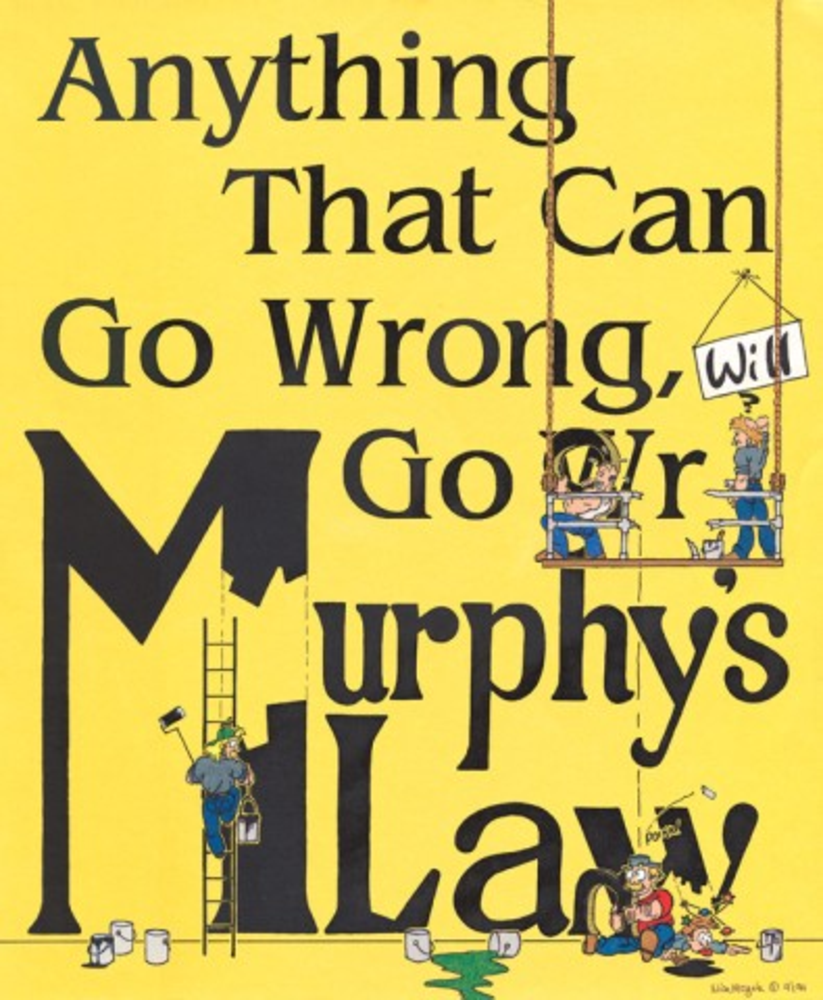
\includegraphics[height=8cm]{Section6/murphys_law}
%
%\end{center}
%
%%\end{frame}
%
%%}
%
%
%\subsection{Type I Error}
%
%%\frame{ \frametitle{Type I error}%\pause
%
%%\vspace{-2 cm}
%
%\begin{itemize}
%  \item A \textbf{Type I error} is when one rejects $H_0$ when in fact $H_0$ is true.
%  \item The probability of making a Type I error is called the \textbf{size} or \textbf{significance level} of the test and is
%  denoted by $\alpha$.
%   \item<3-> It is also known as a \textbf{false positive}.
%\end{itemize}
%
%\iffalse
%\PutAt<1-1>{(2cm,7cm)}{\NormalBox{\parbox[position]{8cm}{\begin{center}\Huge{\alert{TYPE I ERROR}}\end{center}}}}
%\PutAt<2-2>{(2cm,7cm)}{\NormalBox{\parbox[position]{8cm}{\begin{center}\Huge{\alert{SIZE $\alpha$}}\end{center}}}}
%\PutAt<3-3>{(2cm,6cm)}{\NormalBox{\parbox[position]{8cm}{\begin{center}\Huge{\alert{FALSE POSITIVE}}\end{center}}}}
%
%}
%\fi
%\subsection{Type II Error}
%
%%\frame{ \frametitle{Type II error}%\pause
%
%%\vspace{-2 cm}
%
%\begin{itemize}
%  \item A \textbf{Type II error} is when one accepts $H_0$ when in fact $H_0$ is false.
%  \item The probability of making a Type II error is denoted by \textbf{$\beta$}.
%   \item It is also known as a \textbf{false negative}.
%\end{itemize}
%\iffalse
%\PutAt<1-1>{(2cm,7cm)}{\NormalBox{\parbox[position]{8cm}{\begin{center}\Huge{\alert{TYPE II ERROR}}\end{center}}}}
%\PutAt<2-2>{(2cm,7cm)}{\NormalBox{\parbox[position]{8cm}{\begin{center}\Huge{\alert{$\beta$}}\end{center}}}}
%\PutAt<3-3>{(2cm,6cm)}{\NormalBox{\parbox[position]{8cm}{\begin{center}\Huge{\alert{FALSE NEGATIVE}}\end{center}}}}
%
%}
%\fi
%\subsection{Summary Table}
%
%%\frame{ \frametitle{Summary Table}%\pause
%
%%\vspace{-2 cm}
%
%\begin{tabular}{ccc}
%\ &Truth&Truth \\ \hline
%Statistical Decision&$H_0$&$H_a$\\ \hline
%Accept $H_0$&No error&Type II error ($\beta$)\\
%Reject $H_0$&Type I error ($\alpha$)&No error \\ \hline
%\end{tabular}
%\iffalse
%\PutAt<1-1>{(2cm,7cm)}{\NormalBox{\parbox[position]{8cm}{\begin{center}\Huge{\alert{ACCEPT $H_0$}}\end{center}}}}
%\PutAt<2-2>{(2cm,7cm)}{\NormalBox{\parbox[position]{8cm}{\begin{center}\Huge{\alert{REJECT $H_0$}}\end{center}}}}
%%\PutAt<3-3>{(2cm,6cm)}{\NormalBox{\parbox[position]{8cm}{\begin{center}\Huge{\alert{FALSE NEGATIVE}}\end{center}}}}
%
%}
%\fi
%
%\subsection{Parameters for Testing}
%%\begin{frame} \frametitle{Actual Tests (Inference)}%\pause
%
%%\vspace{-2 cm}
%\begin{itemize}
%
%\item Population mean $\mu$ which come from quantitative data.
%
%\item Population proportion $p$ which come from qualitative data.
%
%\end{itemize}
%
%\iffalse
%\PutAt<1-1>{(2cm,6cm)}{\NormalBox{\parbox[position]{8cm}{\begin{center}\Huge{\alert{QUANTITATIVE DATA}}\end{center}}}}
%\PutAt<2-2>{(2cm,6cm)}{\NormalBox{\parbox[position]{8cm}{\begin{center}\Huge{\alert{QUALITATIVE DATA}}\end{center}}}}
%
%\end{frame}
%%________________________________________________________________________
%\fi
%\subsection{Interpretation}
%
%%\frame{ \frametitle{Test Statistic Falls in Rejection Region}%\pause
%
%%\vspace{-2 cm}
%
%\begin{itemize}
%  \item we reject the null hypothesis;
%  \item conclude that the alternative is true;
%  \item and quantify that we are making this conclusion with the possibility of
%  making a 100$\alpha$\% probability of error (Type I error).
%\end{itemize}
%\iffalse
%\PutAt<1-1>{(2cm,6cm)}{\NormalBox{\parbox[position]{8cm}{\begin{center}\Huge{\alert{REJECT $H_0$}}\end{center}}}}
%\PutAt<2-2>{(2cm,6cm)}{\NormalBox{\parbox[position]{8cm}{\begin{center}\Huge{\alert{ACCEPT $H_a$}}\end{center}}}}
%\PutAt<3-3>{(2cm,6cm)}{\NormalBox{\parbox[position]{8cm}{\begin{center}\Huge{\alert{100$\alpha$\% ERROR}}\end{center}}}}
%
%}
%\fi
%%________________________________________________________________________
%
%%\subsection{Interpretation}
%
%%\frame{ \frametitle{Test Statistic Does Not Fall in Rejection Region}%\pause
%
%%\vspace{-2 cm}
%
%\begin{itemize}
%  \item we do not reject the null hypothesis;
%  \item we do not conclude that the null hypothesis is true;
%  \item because in general we do not know the probability $\beta$ of incorrectly accepting $H_0$ (Type II error).
%\end{itemize}
%
%
%\iffalse
\documentclass[12pt]{article}
\usepackage{amsmath}
\usepackage{latexsym}

\addtolength{\textwidth}{1in} \addtolength{\oddsidemargin}{-0.5in}
\addtolength{\textheight}{1.6in} \addtolength{\topmargin}{-0.8in}

\newfont{\tebbb}{msbm10 scaled\magstep1}

\newtheorem{theorem}{Theorem}[section]
\newtheorem{proposition}[theorem]{Proposition}
\newtheorem{lemma}[theorem]{Lemma}
\newtheorem{corollary}[theorem]{Corollary}
\newtheorem{remark}[theorem]{Remark}
\newtheorem{example}[theorem]{Example}
\newcommand{\beq}{\begin{equation}}
\newcommand{\eeq}{\end{equation}}
\newtheorem{definition}[theorem]{Definition}


\newcommand{\cross}[2]{{{\bf{#1}} \times {\bf{#2}}}}
\newcommand{\dotprod}[2]{{{\bf{#1}} \cdot {\bf{#2}}}}
\newcommand{\real}[1]{{\mbox{\tebbb R}}^{#1}}
\newcommand{\norm}[1]{\|{\bf{#1}}\|}
\renewcommand{\theequation}{\thesection.\arabic{equation}}

\baselineskip = 20pt plus 3pt minus 3pt

\begin{document}
\fi
\section{Suggested Exercises}\label{ssec.se3}\markright{\ref{ssec.se3} \titleref{ssec.se3}}
\begin{enumerate}
\item Which hypothesis,the null or the alternative,is the statusquo hypothesis?Which is the research hypothesis?
\item What is a test statistics?
\item Define $\alpha$ and  $\beta$. How do they relate to Type I and Type II errors?
\item If you test a hypothesis and reject the null hypothesis in favor of the alternative hypothesis,does your test prove that the alternative hypothesis is correct?Explain.
\item List all possible results of the combinations of decisions and true states of nature ofr a test of hypothesis.
\end{enumerate}

\iffalse
\begin{enumerate}
\item  Let $A=\left[
\begin{array}{rr}
2 & 3 \\ 3 & 5 \end{array} \right ]$ and calculate:
\begin{enumerate}
\item $A^{-1}$
\item (i) $4A$ \quad (ii) $(4A)^{-1}$
\item (i) $A^t$ \quad (ii) $(A^t)^{-1}$
\item (i) $A^3$ \quad (ii) $A^{-3}.$
\end{enumerate}
\item Let $B= \left[
{\begin{array}{rr}
2 & 5 \\
1 & 3
\end{array}}
 \right]$ and $A$ as above. Find
\begin{enumerate}
\item $B^{-1}$
\item (i) $AB$ \quad (ii) $(AB)^{-1}$ \quad (iii) $B^{-1}A^{-1}$
\end{enumerate}
\item For each of the following calculate the inverse.
\begin{enumerate}
\item $\left[ {\begin{array}{rrr} 1 & 0 & 2 \\ 2 & -1 & 3 \\ 4 & 1 &
8
\end{array}}
 \right]$
\item $\left[ {\begin{array}{rrr} 1 & 2 & 1 \\ 1 & 1 & 1 \\ 3 & -1 &
1
\end{array}}
 \right]$
\item $ \left[ {\begin{array}{rrr} 1 & 3 & -4 \\ 1 & 5 & -1 \\ 3 &
13 & -6
\end{array}}
 \right]
$
\item $\left[ {\begin{array}{rrr} 0 & 1 & 1 \\ 5 & 1 & -1 \\ 2 & -3
& -3
\end{array}}
 \right]$
\item $\left [\begin {array}{rrrr} 1&0&0&0\\2&-2&0&0
\\3&1&-2&0\\1&-1&3&0\end {array}
\right ]$
\item $ \left[ {\begin{array}{rrrr} 1 & 2 & 1 & 0 \\ 0 &
1 & -1 & 0 \\ 1 & 3 & 1 & -2 \\ 1 & 4 & -2 & 4
\end{array}}
\right]$
\end{enumerate}
\item Solve the following system using matrix inversion.
\begin{eqnarray*} x_1+2x_2+x_3&=&1\\
x_2-x_3&=&-1\\ x_1+3x_2+x_3-2x_4&=&-2\\ x_1+4x_2-2x_3+4x_4&=&4
\end{eqnarray*}
\item Let $A= \left[
\begin{array}{rr}
1 & 5 \\
0 & 1
\end{array}
 \right]$, $B= \left[
\begin{array}{rr}
2 & 3 \\
1 & -2
\end{array}
 \right]$ $C= \left[
\begin{array}{rr}
3 & -5 \\
-1 & 2
\end{array}
 \right]$
 $D= \left[
\begin{array}{rr}
-3 & -5 \\
7 & 2
\end{array}
 \right]$  find
\begin{enumerate}
 \item (i) $\det(A)$ \quad (ii) $\det(B)$ \quad (iii) $\det(C)$ \quad (iv) $\det(D)$
 \item (i) $\det(A+B)$ \quad (ii) $\det(A)+\det(B)$
 \item (i) $\det(3A)$ \quad (ii) $\det(B^t)$
 \item (i) $AB$ \quad (ii) $\det(AB)$ \quad (iii) $\det(A)\det(B)$
 \item $\det(D^{-1})$
\end{enumerate}
\item Let $G=\left[
{\begin{array}{rrr}
1 & 0 & 1 \\
2 & 3 & 1 \\
-7 & 0 & -7
\end{array}}
 \right]$,
$H =  \left[
{\begin{array}{rrr}
1 & 2 & 3 \\
4 & 6 & 5 \\
3 & 2 & 7
\end{array}}
 \right]$,
$J =  \left[
{\begin{array}{rrr}
-2 & 4 & -6 \\
3 & -5 & 7 \\
9 & -6 & -3
\end{array}}
 \right]$ find
\begin{enumerate}
\item (i) $\det(G)$ \quad (ii) $\det(G^t)$ \quad
\item $\det(H)$
\item $\det(J)$
\item (i) $\det(HJ)$ (ii) $\det(GJ)$
\end{enumerate}
\item Find $\det(A)$ and $\det(A^{-1})$ for
\begin{align*}
\mathrm{(a)}\ \ A &= \left[ \begin{array}{rrrr} 1 & 2 & 1 & 0 \\ 0 & 1 & -1 & 0
\\ 1 & 3 & 1 & -2 \\ 1 & 4 & -2 & 4 \end{array} \right]&
\mathrm{(b)}\ \ A&= \left[ {\begin{array}{rrrr} 10 & -3 & -3 & -2 \\ 10 & -3 &
-4 & -3 \\ -6 & 2 & 2 & 1 \\ -3 & 1 & 1 & 1 \end{array}} \right]
\end{align*}

\item We have seen that systems of equations can be solved  using either
Gaussian elimination or with ${\bf x}=A^{-1}{\bf b}$. Determine
which of the two methods are appropriate for the following two
systems.
\begin{align*}
\mathrm{(a)}\qquad \quad \quad \ x_1-x_3&=-1& \mathrm{(b)}\ \ 2x_1+x_2-x_3&=6\\
11x_1+2x_2+x_3&=2& 3x_1-x_2&=1\\
3x_1+x_2+3x_3&=1& 9x_2+2x_3&=0
\end{align*}

\end{enumerate}

\section{Answers to activity questions and suggested exercises}
\label{answers3}\markright{\ref{answers3}
\titleref{answers3}}

{\bf Activity questions}

\bigskip

\noindent {\bf \ref{ssec.definv}:}
\begin{enumerate}
\item (a), but not (b).
\item $I$.
\end{enumerate}

\bigskip

\noindent {\bf \ref{ssec.findinv}:}

\begin{enumerate}
\item \begin{enumerate}
\item
\begin{eqnarray*}
& &
\left[ \begin{array}{rrrcrrr} 1 & 0 & 1 & \vline & 1 & 0 & 0\\
                             -1 & 1 & 2 & \vline & 0 & 1 & 0\\
                              2 & 2 & 9 & \vline & 0 & 0 & 1
\end{array} \right]
\\&&\hspace{-12mm}
\overset{\begin{smallmatrix}R_2+R_1\\R_3-2R_1\end{smallmatrix}}{\leadsto}
\left[ \begin{array}{rrrcrrr} 1 & 0 & 1 & \vline & 1 & 0 & 0\\
                              0 & 1 & 3 & \vline & 1 & 1 & 0\\
                              0 & 2 & 7 & \vline & -2 & 0 & 1
\end{array} \right]
\\&&\hspace{-11mm}
\overset{R_3-2R_2}{\leadsto}
\left[ \begin{array}{rrrcrrr} 1 & 0 & 1 & \vline & 1 & 0 & 0\\
                               0 & 1 & 3 & \vline & 1 & 1 & 0\\
                               0 & 0 & 1 & \vline & -4 & -2 & 1
\end{array} \right]
\\&&\hspace{-12mm}
\overset{\begin{smallmatrix}R_1-R_3\\R_2-3R_3\end{smallmatrix}}{\leadsto}
\left[\begin{array}{rrrcrrr} 1 & 0 & 0 & \vline & 5 & 2 & -1\\
                               0 & 1 & 0 & \vline & 13 & 7 & -3\\
                               0 & 0 & 1 & \vline & -4 & -2 & 1
\end{array} \right].
\end{eqnarray*}
The inverse is
$\left[ \begin{array}{rrr} 5&2&-1\\13&7&-3\\-4&-2&1 \end{array} \right]$.
\item
\begin{eqnarray*}&&
\left[ \begin{array}{rrrcrrr} 1 & 0 & 1 & \vline & 1 & 0 & 0\\
                               1 & 1 & 0 & \vline & 0 & 1 & 0\\
                               -1 & 1 & -2 & \vline & 0 & 0 & 1
\end{array} \right]\\
 \overset{\begin{smallmatrix}R_2-R_1\\R_3+R_1\end{smallmatrix}}{\leadsto}
&&\vspace{-10mm}\left[ \begin{array}{rrrcrrr} 1 & 0 & 1 & \vline & 1 & 0 & 0\\
                              0 & 1 & -1 & \vline & -1 & 1 & 0\\
                              0 & 1 & -1 & \vline & -1 & 0 & 1
\end{array} \right]\\ \\
\overset{R_3-R_2}{\leadsto}
&&\vspace{-10mm}\left[ \begin{array}{rrrcrrr} 1 & 0 & 1 & \vline & 1 & 0 & 0\\
                               0 & 1 & -1 & \vline & -1 & 1 & 0\\
                               0 & 0 & 0 & \vline & 0 & -1 & 1
\end{array} \right].
\end{eqnarray*}
The matrix does not reduce to $I$ so $\exists$ no inverse.
\item
\begin{eqnarray*}
&&
\left[ \begin{array}{rrrrcrrrr}  1 & 0 & 0 & 0 & \vline & 1 & 0 & 0 & 0\\
                                 0 & 0 & 0 & 1 & \vline & 0 & 1 & 0 & 0\\
                                 0 & 0 & 1 & 0 & \vline & 0 & 0 & 1 & 0\\
                                 0 & 1 & 0 & 0 & \vline & 0 & 0 & 0 & 1
\end{array} \right] \\ \\\overset{R_2\leftrightarrow R_4}{\leadsto}
&&\vspace{-10mm}\left[ \begin{array}{rrrrcrrrr}  1 & 0 & 0 & 0 & \vline & 1 & 0 & 0 & 0\\
                                 0 & 1 & 0 & 0 & \vline & 0 & 0 & 0 & 1\\
                                 0 & 0 & 1 & 0 & \vline & 0 & 0 & 1 & 0\\
                                 0 & 0 & 0 & 1 & \vline & 0 & 1 & 0 & 0
\end{array} \right].
\end{eqnarray*}
 Hence this matrix is it's own inverse.

\end{enumerate}
\end{enumerate}

\bigskip

\noindent {\bf \ref{ssec.propinv}:}\\
\vspace{0.1\baselineskip}

\noindent {\bf Hints: } To prove number 5, what does
$(A^{-1})(A^{-1})^{-1}$ equal?  To prove number 7, use the exact
same method shown in the notes, except that you now multiply
$(kA)(\frac{1}{k}A^{-1}$).

\bigskip

\noindent {\bf \ref{ssec.syseinv}:}
\begin{enumerate}
\item $A^{-1}=\left [ \begin{array}{rrr}\vspace{1mm}
                                1&0&1\\ \vspace{1mm}
                                1&1&\frac{5}{2}\\
                                0&0&-\frac{1}{2} \end{array} \right
                                ]$,\  $x_1=\left [ \begin{array}{r}\vspace{1mm}
                                -2\\ \vspace{1mm}-\frac{5}{2}\\ \frac{3}{2}
                                \end{array} \right ]$,\ $x_2=\left [ \begin{array}{r} \vspace{1mm}
                                -11\\ \vspace{1mm} -\frac{13}{2}\\ \frac{1}{2}
                                \end{array} \right ]$.
\item Same as 1.

\item ${\bf x}={\bf 0}$.

\item If any other {\bf b} are introduced into the problem, by
theorem \ref{eq2invert} we know that the system will be consistent
and have exactly one solution for every {\bf b}.
\end{enumerate}

\noindent {\bf \ref{sec.det}:}
\begin{enumerate}
\item \begin{itemize} \item[(i)]
\begin{itemize}
\item[(a)] $2\left| \begin{array}{rr}2&-2\\0&1\end{array} \right| +
\left| \begin{array}{rr}3&-2\\0&1\end{array} \right| +
3 \left| \begin{array}{rr}3&2\\0&0\end{array} \right| = 4+3+0 = 7$
\item[(b)] $1\left| \begin{array}{rr}3&-2\\0&1\end{array} \right| +
2\left| \begin{array}{rr}2&3\\0&1\end{array} \right| +
0\left| \begin{array}{rr}2&3\\3&-2\end{array} \right| = 3+4+0 = 7$
\end{itemize}
\item[(ii)]
\begin{itemize}
\item[(a)] $2\left| \begin{array}{rr}1&2\\8&3\end{array} \right| -
3\left| \begin{array}{rr}0&2\\0&3\end{array} \right| +
2\left| \begin{array}{rr}0&1\\0&8\end{array} \right| = -26+0+0 = -26$
% START HERE
\item[(b)] $-3\left| \begin{array}{rr}0&2\\0&3\end{array} \right| +
1\left| \begin{array}{rr}2&2\\0&3\end{array} \right| -
8\left| \begin{array}{rr}2&2\\0&2\end{array} \right| = 0+6-32 = -26$
\end{itemize}
\end{itemize}
\item Expand matrix (i) along the bottom row
$$
\left| \begin{array}{rr}2&-1\\3&2\end{array}\right|
$$
Expand matrix (ii) along the bottom row
$$
2 \left| \begin{array}{rr}1&2\\8&3\end{array} \right| = 2(3-16) = -26
$$
\end{enumerate}

\noindent {\bf \ref{ssec.propdet}:}
\begin{enumerate}
\item
\begin{enumerate}
\item
$$
\begin{vmatrix}2&2&1\\2&1&1\\1&2&1\end{vmatrix} \overset{R_1 - R_3}{\leadsto}
\begin{vmatrix}1&0&0\\2&1&1\\1&2&1\end{vmatrix} = \begin{vmatrix}1&1\\2&1\end{vmatrix} = 1-2 =-1
$$
\item
\begin{eqnarray*}
\left| \begin{array}{rrrr} 1&2&7&5\\2&1&3&10\\4&-1&-3&20\\8&3&9&39
\end{array} \right|
&& \hspace{-5mm}\overset{\begin{smallmatrix}C_4 -
5C_1\\C_3-3C_2\end{smallmatrix}}{\leadsto} \quad \left|
\begin{array}{rrrr} 1&2&1&0\\2&1&0&0\\4&-1&0&0\\8&3&0&-1
\end{array} \right|\\
&=&
- \left| \begin{array}{rrr} 1&2&1\\2&1&0\\4&-1&0\end{array} \right| \\
&=& - \left| \begin{array}{rr}2&1\\4&-1\end{array} \right| \\&=&
-(-2-4) = 6
\end{eqnarray*}
\end{enumerate}
\item
\begin{enumerate}
\item -3
\item 270
\item -60
\item Not enough information
\end{enumerate}
\end{enumerate}
\noindent {\bf \ref{ssec.adjoint}:}  $A$ is invertible, since
det($A$)=17;  det($A^{-1}$)$=\frac{1}{17}$.


\bigskip

\noindent {\bf Suggested Exercises}

\begin{enumerate}
\item
\begin{enumerate}\item$ \left[ {\begin{array}{rr}5&-3\\-3&2 \end{array}}
\right]$\\
\item(i) $\left[ {\begin{array}{rr}8&12\\12&20\end{array}}
 \right]$\quad
(ii) $\left[ {\begin{array}{rr} \frac {5}{4}  & -\frac {3}{4}\\ -\frac {3}{4}  & \frac {1}{2}
\end{array}} \right]$
\item (i) $\left[ {\begin{array}{rr} 2 & 3 \\ 3 & 5 \end{array}}
\right]$ \quad (ii) $\left[ {\begin{array}{rr} 5 & -3 \\ -3 &
2\end{array}} \right]$
\item (i) $\left[ {\begin{array}{rr} 89 &
144
\\ 144 & 233
\end{array}}
 \right]$\quad
(ii) $
 \left[
{\begin{array}{rr}
233 & -144 \\
-144 & 89
\end{array}}
 \right]$
 \end{enumerate}

\item \begin{enumerate}
\item $ \left[
\begin{array}{rr}
3 & -5 \\
-1 & 2
\end{array}
 \right]$\\
\item (i) $\left[ {\begin{array}{rr} 7 & 19 \\ 11 & 30
\end{array}}
 \right]$ \quad (ii) $ \left[
{\begin{array}{rr}
30 & -19 \\
-11 & 7
\end{array}}
 \right]$ \quad (iii) $ \left[ {\begin{array}{rr} 30 & -19 \\ -11 & 7
\end{array}}
 \right]$
 \end{enumerate}
\item \begin{enumerate}
\item $ \left[ {\begin{array}{rrr} -11 & 2 & 2 \\ -4 & 0 & 1 \\ 6 &
-1 & -1
\end{array}}
 \right]
$
\item $\left[ {\begin{array}{rrr}\vspace{1mm} 1 & -\frac {3}{2}& \frac {1}{2}\\ \vspace{1mm}
1 & -1 & 0 \\ -2 & \frac {7}{2}  & -\frac {1}{2}
\end{array}}
 \right]$
\item Not Possible Singular matrix
\item $\left[ {\begin{array}{rrr}\vspace{1mm} \frac {3}{2} & 0 & \frac
{1}{2}\\ \vspace{1mm} -\frac {13}{4}  & \frac {1}{2} & -\frac {5}{4}  \\ \frac
{17}{4} & -\frac {1}{2} & \frac {5}{4}
\end{array}}
 \right]$
\item Not Possible \item $\left[ {\begin{array}{rccc} 10 & 10 & -6 &
-3
\\ -3 & -3 & 2 & 1 \\  -3 & -4  &
2& 1 \\-1 & -\frac{3}{2} & \frac{1}{2} & \frac{1}{2}
\end{array}}
\right]$
\end{enumerate}
\item $x_1=0,\ x_2=0,\ x_3=1,\ x_4=\tfrac{3}{2}$
\item
\begin{enumerate}
\item (i) 1 (ii) -7 (iii) 1 (iv) 29
\item (i) -11 (ii) -6
\item (i) 9 (ii) -7
\item (i) $ \begin{vmatrix} 7 & -7 \\1 & -2 \end{vmatrix}$ (ii) -7 (iii) -7
\item $\tfrac{1}{29}$
\end{enumerate}
\item
\begin{enumerate}
\item (i) 0 (ii) 0
\item -24
\item 12
\end{enumerate}
\item
\begin{enumerate}
\item (i) 2 (ii) $\frac{1}{2}$
\item (i) 1 (ii) 1
\end{enumerate}
\item
\begin{enumerate}
\item The determinant of the system is $0$, therefore $A$ is not
invertible and the system must be solved using Gaussian
elimination.
\item The determinant is not 0; either method works.
\end{enumerate}
\end{enumerate}

%\end{document}
\fi

%\iffalse
%\PutAt<1-1>{(2cm,6cm)}{\NormalBox{\parbox[position]{8cm}{\begin{center}\Huge{\alert{DO NOT REJECT $H_0$}}\end{center}}}}
%\PutAt<2-2>{(2cm,6cm)}{\NormalBox{\parbox[position]{8cm}{\begin{center}\Huge{\alert{RESERVE JUDGEMENT ON $H_0$}}\end{center}}}}
%\PutAt<3-3>{(2cm,6cm)}{\NormalBox{\parbox[position]{8cm}{\begin{center}\Huge{\alert{DO NOT KNOW $\beta$}}\end{center}}}}
%
%}
%
%\subsection{Exercises}
%
%\begin{frame} \frametitle{Exercises}%\pause
%
%\noindent 11th edition, p. 329:  6.1--6.7.
%
%\bigskip
%
%\noindent 10th edition, p. 350:  6.1--6.7.
%
%\end{frame}
%
%%________________________________________________________________________
%\fi
%
%\section{Large Sample Test for a Single Mean}
%
%\subsection{Large Sample Test for a Single Mean}
%
%%\frame{ \frametitle{Hypothesis Test for a Single Mean}%\pause
%
%%\vspace{-1.5 cm}
%
%For a given population mean $\mu$ we want to formulate a null hypothesis with respect to
%some fixed level, thus
%\[H_0:  \ \mu = \mu_0.\]
%Then we can have,
%
%\begin{itemize}
%  \item A \textbf{one tailed, upper test} where $H_a$ says $\mu > \mu_0$.
%  \item A \textbf{one tailed, lower test} where $H_a$ says $\mu < \mu_0$.
%  \item A \textbf{two tailed test} where $H_a$ says $\mu \neq \mu_0$.
%\end{itemize}
%\iffalse
%\PutAt<1-1>{(2cm,7cm)}{\NormalBox{\parbox[position]{8cm}{\begin{center}\Huge{\alert{$\mu > \mu_0$}}\end{center}}}}
%\PutAt<2-2>{(2cm,7cm)}{\NormalBox{\parbox[position]{8cm}{\begin{center}\Huge{\alert{$\mu > \mu_0$}}\end{center}}}}
%\PutAt<3-3>{(2cm,7cm)}{\NormalBox{\parbox[position]{8cm}{\begin{center}\Huge{\alert{$\mu \neq \mu_0$}}\end{center}}}}
%
%}
%\fi
%\subsection{Test Statistic}
%
%%\frame{ \frametitle{Test Statistic}%\pause
%
%%\vspace{-2 cm}
%
%Let $x_1,\ldots , x_n$ be a random sample from a population that has unknown mean $\mu$
%and standard deviation $\sigma$.  Compute,
%\begin{itemize}
%  \item the sample mean
%  \item the sample standard deviation
%  \item test statistic
%\end{itemize}
%\iffalse
%\PutAt<1-1>{(2cm,6cm)}{\NormalBox{\parbox[position]{8cm}{\begin{center}\Huge{$\bar{x}=\frac1n \sum x_i$}\end{center}}}}
%\PutAt<2-2>{(1cm,6cm)}{\NormalBox{\parbox[position]{10cm}{\begin{center}\Huge{$s=\sqrt{\frac{1}{n-1}\sum \left(x_i -\bar{x}\right)^2}$}\end{center}}}}
%\PutAt<3-3>{(2cm,6cm)}{\NormalBox{\parbox[position]{8cm}{\begin{center}\Huge{$z= \frac{\bar{x}-\mu_0}{s/\sqrt{n}}$}\end{center}}}}
%
%
%}
%\fi
%\subsection{Rejection Region}
%
%%\frame{ \frametitle{Rejection Region - One Tailed Test}%\pause
%
%%\vspace{-2 cm}
%
%Fix $\alpha > 0$ (usually $\alpha = 0.05$) so that
%\[P\left(z > z_\alpha \right) = P\left(z <  -z_\alpha \right) = \alpha \]
%where $z$ denotes a standard normal random variable:
%\begin{itemize}
%  \item one tailed upper test, reject $H_0:  \ \mu = \mu_0$ if
%  \item one tailed lower test, reject $H_0:  \ \mu = \mu_0$ if
%\end{itemize}
%\iffalse
%\PutAt<1-1>{(2cm,6cm)}{\NormalBox{\parbox[position]{8cm}{\begin{center}\Huge{$z= \frac{\bar{x}-\mu_0}{s/\sqrt{n}} > z_\alpha$}\end{center}}}}
%\PutAt<2-2>{(2cm,6cm)}{\NormalBox{\parbox[position]{10cm}{\begin{center}\Huge{$z= \frac{\bar{x}-\mu_0}{s/\sqrt{n}} < -z_\alpha$}\end{center}}}}
%
%
%
%}
%\fi
%\subsection{Rejection Region}
%
%%\frame{ \frametitle{Rejection Region - Two Tailed Test}%\pause
%
%%\vspace{-2 cm}
%
%Fix $\alpha > 0$ (usually $\alpha = 0.05$) so that
%\[P\left(z > z_{\alpha/2} \right) = P\left(z <  -z_{\alpha/2} \right) = {\alpha/2} \]
%where $z$ denotes a standard normal random variable:
%\begin{itemize}
%%  \item<1-> two tailed test, reject $H_0:  \ \mu = \mu_0$ if
%  \item two tailed test, reject $H_0:  \ \mu = \mu_0$ if
%\end{itemize}
%
%%\PutAt<1-1>{(2cm,6cm)}{\NormalBox{\parbox[position]{8cm}{\begin{center}\Huge{$z= \frac{\bar{x}-\mu_0}{s/\sqrt{n}} > z_\alpha/2$}\end{center}}}}
%%\PutAt<2-2>{(2cm,6cm)}{\NormalBox{\parbox[position]{10cm}{\begin{center}\Huge{$z= \frac{\bar{x}-\mu_0}{s/\sqrt{n}} < -z_\alpha/2$}\end{center}}}}
%%\PutAt<2-2>{(2cm,6cm)}{\NormalBox{\parbox[position]{10cm}{\begin{center}\Huge{$|z|= \left|\frac{\bar{x}-\mu_0}{s/\sqrt{n}}\right| > z_{ \alpha/2}$}\end{center}}}}
%
%
%
%%}
%
%\subsection{Interpretation}
%
%%\frame{ \frametitle{Test Statistic Falls in Rejection Region}%\pause
%
%%\vspace{-2 cm}
%
%\begin{itemize}
%  \item we reject the null hypothesis;
%  \item conclude that the alternative is true;
%  \item and quantify that we are making this conclusion with the possibility of
%  making a 100$\alpha$\% probability of error (Type I error).
%\end{itemize}
%\iffalse
%\PutAt<1-1>{(2cm,6cm)}{\NormalBox{\parbox[position]{8cm}{\begin{center}\Huge{\alert{REJECT $H_0$}}\end{center}}}}
%\PutAt<2-2>{(2cm,6cm)}{\NormalBox{\parbox[position]{8cm}{\begin{center}\Huge{\alert{ACCEPT $H_a$}}\end{center}}}}
%\PutAt<3-3>{(2cm,6cm)}{\NormalBox{\parbox[position]{8cm}{\begin{center}\Huge{\alert{100$\alpha$\% ERROR}}\end{center}}}}
%
%}
%%________________________________________________________________________
%
%%\subsection{Interpretation}
%
%\frame{ \frametitle{Test Statistic Does Not Fall in Rejection Region}%\pause
%
%\vspace{-2 cm}
%\fi
%\begin{itemize}
%  \item we do not reject the null hypothesis;
%  \item we do not conclude that the null hypothesis is true;
%  \item because in general we do not know the probability $\beta$ of incorrectly accepting $H_0$ (Type II error).
%\end{itemize}
%\iffalse
%\PutAt<1-1>{(2cm,6cm)}{\NormalBox{\parbox[position]{8cm}{\begin{center}\Huge{\alert{DO NOT REJECT $H_0$}}\end{center}}}}
%\PutAt<2-2>{(2cm,6cm)}{\NormalBox{\parbox[position]{8cm}{\begin{center}\Huge{\alert{RESERVE JUDGEMENT ON $H_0$}}\end{center}}}}
%\PutAt<3-3>{(2cm,6cm)}{\NormalBox{\parbox[position]{8cm}{\begin{center}\Huge{\alert{DO NOT KNOW $\beta$}}\end{center}}}}
%
%}
%\fi
%\subsection{Examples}
%
%%\begin{frame} \frametitle{Examples}%\pause
%
%Will be discussed in class.
%
%%\end{frame}
%




\subsection{Exercises}
\begin{enumerate}
\item Suppose $P(A)=0.5$,$P(B)=0.8$,and $P(A\bigcap B)=0.4$.Find the following probabilities:
\begin{enumerate}
\item Find $P(A^{c})$ 
\item Find $P(A\bigcup B)$
\item Find $P(A\bigcap B^{c})$
\end{enumerate}

\item An experiment is conducted in which the outcomes of each of the two variables are observed.The two variables are Gender \{Male,Female\} and Age\{$\leq 30$,30-50,$\geq50$\}.The probabilities associated with each of the six possible outcome pairs are given as follows:
\begin{center}
\begin{tabular}{|c|c|c|c|}\hline
             &$\leq 30$&30-50&$\geq50$\\ \hline   
Male         &0.50     &0.10 &0.05\\ \hline
Female       &0.25     &0.07 &0.03\\ \hline
\end{tabular}
\end{center}
\begin{enumerate}
\item Find $P$(\{Male\})
\item Find $P$(\{Female or 30-50\})
\item Find $P$(\{$\leq$ 30\})
\item Find $P$(\{$\leq$ 30 and Female\})
\end{enumerate}


\item A pair of fair dice is tossed.Considering the following events:\\
%\begin{description}
$A$: \{The sum of the dots on the up faces of the two dice is 8\}.\\
$B$: \{at least one of the two dice showing is 3\}.

% \end{description}

\begin{enumerate}
\item Identify the sample points in the events $A,B,A\bigcap B,A\bigcup B$,and $A^{c}$.
\item Find the corresponding probabilities in part (a). 
\item Apply additive rule to $P$($A \bigcup B$).
\item Are the events $A$ and $B$ mutually exclusive?Why?
\end{enumerate}



\iffalse
\item Two balls are drawn at random and without replacement from a box containing two blue balls and two red balls.
\begin{enumerate}
\item List the sample points for this experiment.
\item Assign probabilities to the sample points.
\item Find the probability of the following events:
\begin{enumerate}
\item \{two red balls are drawn\}
\item \{One red and one blue are drawn\}
\item \{two balls with the same color are drawn\}
\end{enumerate}
\item The diagram below describes the sample space of a particular experiment and events A and B.
\begin{enumerate}
\item What is the name of the diagram?
\item Assume the sample points have the same probability.Find P(A),P(B) and P(C) .

\end{enumerate}
\end{enumerate}
\fi
%\item Show that if two $n \times n$ matrices $L$, $M$ are symmetric, then so are $L+M$ and $kL$.

\end{enumerate}
%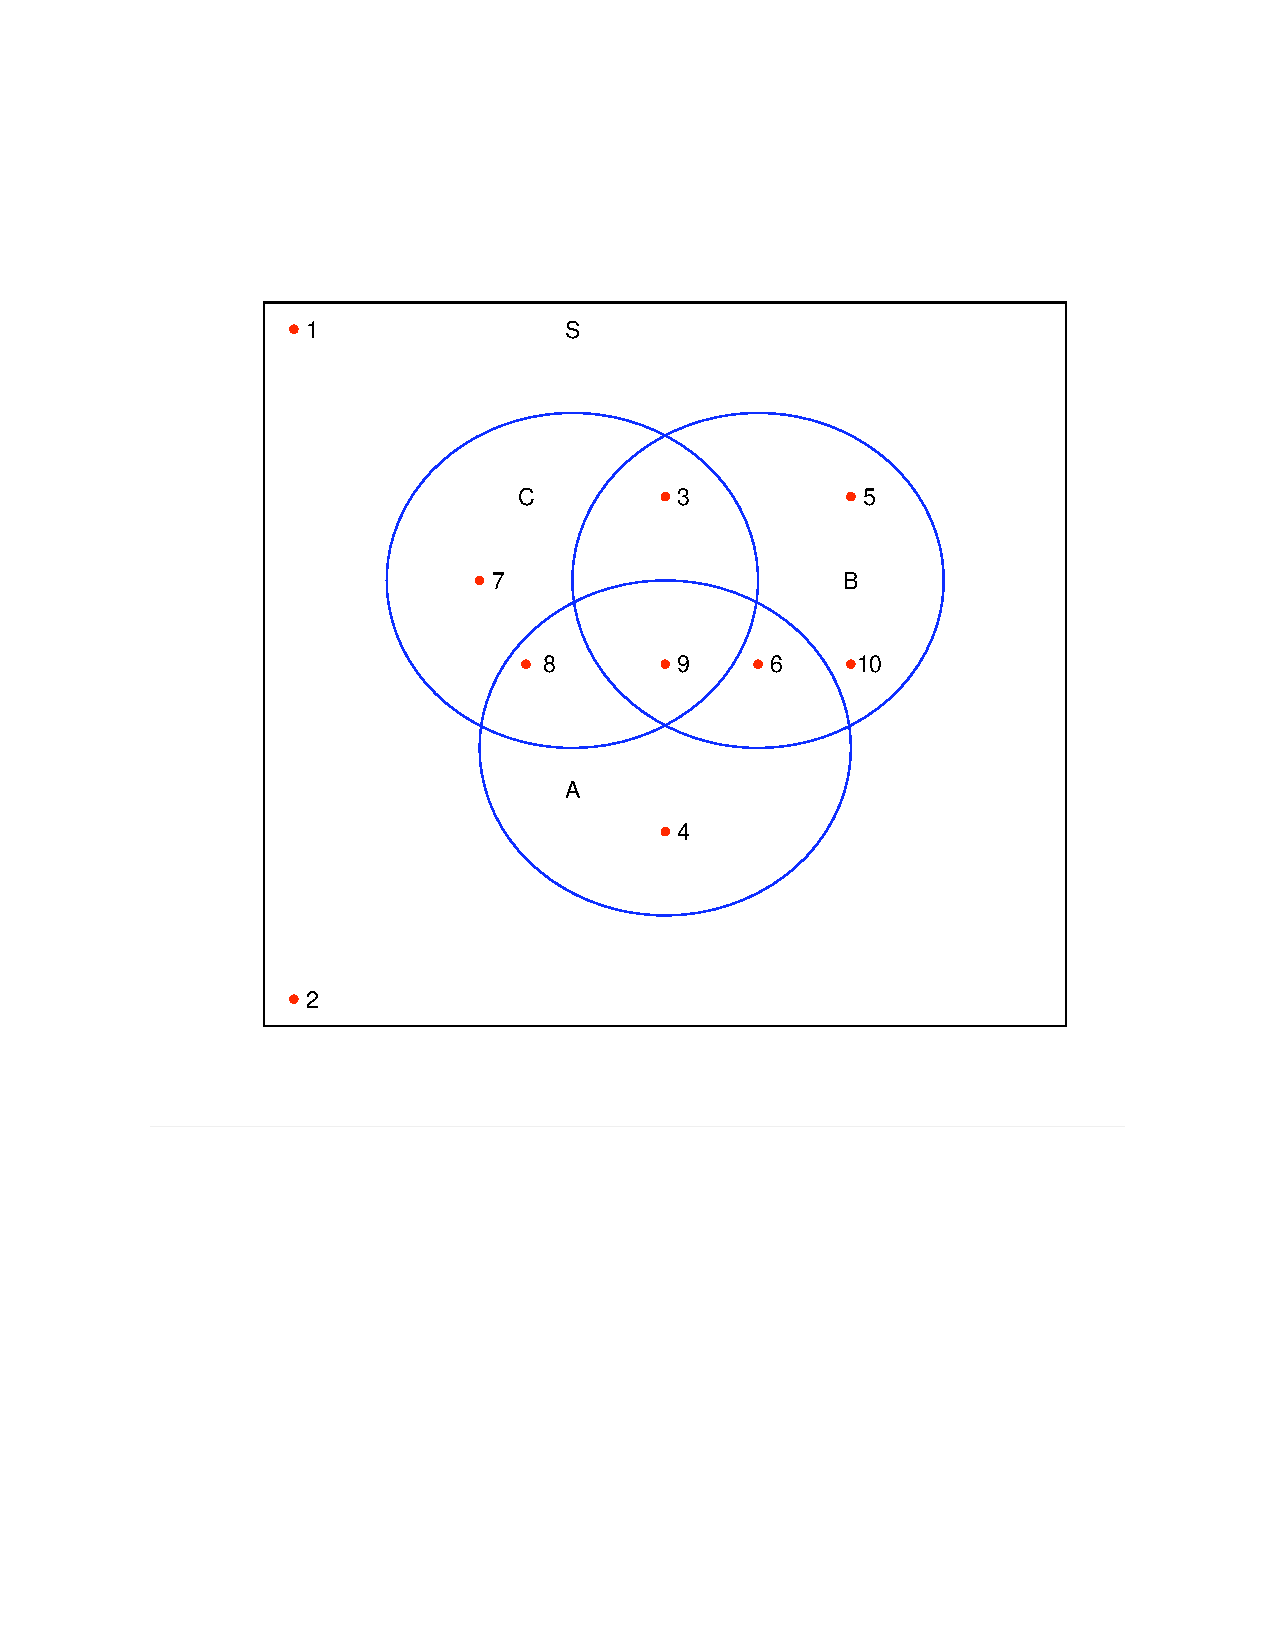
\includegraphics[height=12cm]{a2-fig-2}
\iffalse
\label{se1} \markright{\ref{se1}
\titleref{se1}}
For the following exercises, let\\ $A=[1\ 2],\ B=\left[
\begin{array}{c}3\\2 \end{array}\right ],\ C=\left [\begin
{array}{rr} 1&-2\\2&-3\end {array} \right ],\ D=\left [\begin
{array}{rr} -2&-5\\1&3\end {array} \right ],\\ E=\left [\begin
{array}{rr} 1&5\\3&8
\\2&1\end {array}\right ],\
F=\left [\begin {array}{rrr} 2&-4&1\\6&-9&1\\4&1&6\\1&7&-5\end {array}\right],\
G=\left [\begin {array}{rrr} 1&2&6\\2&-3&7
\\4&-1&3\end {array}\right ],\\
H=\left [\begin {array}{rrr} 1&0&0\\0&1&0
\\-1&0&0\end {array}\right ],\
I=\left [\begin {array}{rrr} 1&0&0\\0&1&0
\\0&0&1\end {array}\right ],\
K=\left [\begin {array}{rrrr} 1&-2&4&7\\2&3&5&-4
\\1&4&2&1\\-2&1&9&4\end {array}
\right ].$
\bigskip

\begin{enumerate}
\item Which of the following operations are not defined? If they
are defined, what is the size of the resulting matrix
\begin{enumerate}
\item $AC$
\item $CA$
\item $KF^t$
\item $KF$
\item $EB+A^t$
\item $E(H+I)$
\end{enumerate}
\item Find: a) $C+D$\quad b) $D+C$ \quad  c) $G+H$ \quad
d) $D-3C$ \quad e) $2D$
\item Find:
\begin{enumerate} \item $AB$ and $BA$
\item $(C+2D)+BA$ and $C+(2D+BA)$
\item $DC$, $ED$, $(ED)C$ and $E(DC)$
\item $FH+FG$ and $F(G+H)$
\item $G^t$, $H^t$, $(GH)^t$, $G^tH^t$ and $H^tG^t$.
\end{enumerate}
\item Find: $KF$, $FG$ and $FH$.
\item Find tr($K$), tr($I$) and tr($E$).
\item Find $C^3$ and $H^2$.
\item Find $I-H$  and $(I-H)^2$.
\item If $f(x)=x^{2} +2x+2$, $g(x)=x^{2}-x-1$, find
\begin{enumerate} \item $f(C), {\rm (b)}~f(D), {\rm (c)}~g(C), {\rm (d)}~g(D)$.
\end{enumerate}
\item Show that if two $n \times n$ matrices $L$, $M$ are symmetric, then so are $L+M$ and $kL$.

\end{enumerate}



\iffalse
\section{Maple Exercises (optional)}

As in the previous session, first open the linear algebra package.

\begin{maplegroup}
\begin{mapleinput}
\mapleinline{active}{1d}{with(linalg):}{%
}
\end{mapleinput}

\end{maplegroup}
\bigskip

In this chapter, matrix operations and the matrix form of a linear
system ( $A{\bf x}={\bf b}$) were introduced.

We will begin this session by giving a second command to construct
a matrix (the first command was given during the previous Maple
session).

\bigskip

\begin{maplegroup}
\begin{mapleinput}
\mapleinline{active}{1d}{A := matrix(3,3, [1,2,3,2,3,4,3,4,5]);}{%
}
\end{mapleinput}

\mapleresult
\begin{maplelatex}
\[
A :=  \left[ {\begin{array}{rrr} 1 & 2 & 3 \\ 2 & 3 & 4 \\ 3 & 4 &
5
\end{array}}
 \right]
\]
\end{maplelatex}

\end{maplegroup}
\begin{maplegroup}
\begin{mapleinput}
\mapleinline{active}{1d}{B:=matrix(3,3,[2,5,7,13,3,5,6,7,8]);}{%
}
\end{mapleinput}

\mapleresult
\begin{maplelatex}
\[
B :=  \left[ {\begin{array}{rrr} 2 & 5 & 7 \\ 13 & 3 & 5 \\ 6 & 7
& 8
\end{array}}
 \right]
\]
\end{maplelatex}

\end{maplegroup}
\begin{maplegroup}
\begin{mapleinput}
\mapleinline{active}{1d}{C:=matrix(4,3,[1,3,5,7,9,0,8,6,4,2,1,7]);}{%
}
\end{mapleinput}

\mapleresult
\begin{maplelatex}
\[
C :=  \left[ {\begin{array}{rrr} 1 & 3 & 5 \\ 7 & 9 & 0 \\ 8 & 6 &
4 \\ 2 & 1 & 7
\end{array}}
 \right]
\]
\end{maplelatex}

\end{maplegroup}
\begin{maplegroup}
\begin{mapleinput}
\mapleinline{active}{1d}{E:=matrix(3,4,[3,4,7,6,9,2,8,2,6,8,3,12]);}{%
}
\end{mapleinput}

\mapleresult
\begin{maplelatex}
\[
E :=  \left[ {\begin{array}{rrrr} 3 & 4 & 7 & 6 \\ 9 & 2 & 8 & 2
\\ 6 & 8 & 3 & 12
\end{array}}
 \right]
\]
\end{maplelatex}

\end{maplegroup}
\bigskip

{\bf Note:} You can not let a matrix be $D$, a Maple error will
result.

Now that we have a few matrices at hand, we will perform some
matrix operations on them. First, scalar multiplication and matrix
addition. These operations are accomplished using the commands:
scalarmul(\emph{matrix name}, \emph{scalar value}) and
matadd(\emph{matrix name},\emph{matrix name}).

\bigskip

\begin{maplegroup}
\begin{mapleinput}
\mapleinline{active}{1d}{scalarmul(B,2);}{%
}
\end{mapleinput}

\mapleresult
\begin{maplelatex}
\[
 \left[
{\begin{array}{rrr} 4 & 10 & 14 \\ 26 & 6 & 10 \\ 12 & 14 & 16
\end{array}}
 \right]
\]
\end{maplelatex}

\end{maplegroup}
\begin{maplegroup}
\begin{mapleinput}
\mapleinline{active}{1d}{matadd(A , B);}{%
}
\end{mapleinput}

\mapleresult
\begin{maplelatex}
\[
 \left[
{\begin{array}{rrr} 3 & 7 & 10 \\ 15 & 6 & 9 \\ 9 & 11 & 13
\end{array}}
 \right]
\]
\end{maplelatex}

\end{maplegroup}
\bigskip

The `matadd' command can also be used to add scalar multiples of
one matrix to another matrix in the following way.
\bigskip

\begin{maplegroup}
\begin{mapleinput}
\mapleinline{active}{1d}{matadd(3*A,-B);}{%
}
\end{mapleinput}

\mapleresult
\begin{maplelatex}
\[
 \left[
{\begin{array}{rrr} 1 & 1 & 2 \\ -7 & 6 & 7 \\ 3 & 5 & 7
\end{array}}
 \right]
\]
\end{maplelatex}

\end{maplegroup}
\begin{maplegroup}
Matrix multiplication is performed using the `multiply' command.

\end{maplegroup}
\begin{maplegroup}
\begin{mapleinput}
\mapleinline{active}{1d}{multiply(A,B);}{%
}
\end{mapleinput}

\mapleresult
\begin{maplelatex}
\[
 \left[
{\begin{array}{rrr} 46 & 32 & 41 \\ 67 & 47 & 61 \\ 88 & 62 & 81
\end{array}}
 \right]
\]
\end{maplelatex}

\end{maplegroup}
\begin{maplegroup}
\begin{mapleinput}
\mapleinline{active}{1d}{multiply(A,B,E);}{%
}
\end{mapleinput}

\mapleresult
\begin{maplelatex}
\[
 \left[
{\begin{array}{rrrr} 672 & 576 & 701 & 832 \\ 990 & 850 & 1028 &
1228 \\ 1308 & 1124 & 1355 & 1624
\end{array}}
 \right]
\]
\end{maplelatex}

\end{maplegroup}
\bigskip

As shown in the previous section, Maple can be used to solve
systems of equations using the row reduction technique. A second
method uses the `linsolve' command. If we have the system $A{\bf
x}={\bf b}$, this command solves for {\bf x}. This command will be
demonstrated with the matrix $B$ from above, and a row matrix or
vector, $b$.

\bigskip

\begin{maplegroup}
\begin{mapleinput}
\mapleinline{active}{1d}{b:=vector([2,3,6]);}{%
}
\end{mapleinput}

\mapleresult
\begin{maplelatex}
\[
b := [2, \,3, \,6]
\]
\end{maplelatex}

\end{maplegroup}
\begin{maplegroup}
\begin{mapleinput}
\mapleinline{active}{1d}{linsolve(B,b);}{%
}
\end{mapleinput}

\mapleresult
\begin{maplelatex}
\[
 \left[  \! {\displaystyle \frac {29}{119}} , \,{\displaystyle
\frac {260}{119}} , \,{\displaystyle -\frac {160}{119}}  \!
 \right]
\]
\end{maplelatex}

\end{maplegroup}
\bigskip

Try solving the same system using the techniques and commands of
the previous Maple session.

The transpose of a matrix was also defined in this section. On
Maple, the transpose of a matrix is found with the `transpose'
command.
\bigskip

\begin{maplegroup}
\begin{mapleinput}
\mapleinline{active}{1d}{transpose(A);}{%
}
\end{mapleinput}

\mapleresult
\begin{maplelatex}
\[
 \left[
{\begin{array}{rrr} 1 & 2 & 3 \\ 2 & 3 & 4 \\ 3 & 4 & 5
\end{array}}
 \right]
\]
\end{maplelatex}

\end{maplegroup}
\begin{maplegroup}
\mapleresult
\begin{maplettyout}
\end{maplettyout}

\end{maplegroup}
\bigskip

Again you might want to try some other examples for yourself.  You
can also combine the commands to simplify long strings of
calculations. \fi

\section{Answers to activity questions and suggested exercises}
\label{answers2}

{\bf Activity questions}

\bigskip

\noindent {\bf \ref{ssec.arith}:} \quad 1.Yes.

\bigskip

\noindent{\bf \ref{ssec.propma}:} \quad Yes.

\bigskip


\noindent{\bf Suggested exercises}

\begin{enumerate}
\item \begin{enumerate}
\item $1 \times 2$
\item undefined
\item undefined
\item $4 \times 3$
\item undefined
\item undefined \end{enumerate}
\item a) $\left [\begin {array}{rr} -1&-7\\3&0\end {array}
\right ]$
b) $\left [\begin {array}{rr} -1&-7\\3&0\end {array}
\right ]$
c) $\left [\begin {array}{rrr} 2&2&6\\2&-2&7
\\3&-1&3\end {array}\right ]$
\\
d) $\left [\begin {array}{rr} -5&1\\-5&12\end {array} \right ]$ e)
$\left [\begin {array}{rr} -4&-10\\2&6\end {array} \right ]$
\item  \begin{enumerate} \item $7$, $\quad \left [\begin {array}{rr} 3&6\\2&4\end {array} \right ]$
\item $\left [\begin {array}{rr} 0&-6\\6&7\end {array}
\right ]$
\item  $\left [\begin {array}{rrr} -12&19\\7&-11\end {array}
\right ]$,  $\left [\begin {array}{rrr} 3&10\\2&9
\\-3&-7\end {array}\right ]$,  $\left [\begin {array}{rr} 23&-36\\20&-31
\\-17&27\end {array}\right ]$,  $\left [\begin {array}{rr} 23&-36\\20&-31
\\-17&27\end {array}\right ]$
\item $\left [\begin {array}{rrr} -1&11&-13\\-3&29&-24
\\28&0&49\\1&-7&40\end {array}
\right ]$, \quad $\left [\begin {array}{rrr} -1&11&-13\\-3&29&-24
\\28&0&49\\1&-7&40\end {array}
\right ]$
\item $G^t=\left [\begin {array}{rrr} 1&2&4\\2&-3&-1
\\6&7&3\end {array}\right ]$, \quad $H^t=\left [\begin {array}{rrr} 1&0&-1\\0&1&0
\\0&0&0\end {array}\right ]$, \\$(GH)^t=\left [\begin {array}{rrr} -5&-5&1\\2&-3&-1
\\0&0&0\end {array}\right ]$ \\

$G^tH^t=\left [\begin {array}{rrr} 1&2&-1\\2&-3&-2
\\6&7&-6\end {array}\right ]$, \quad $H^tG^t=\left [\begin {array}{rrr} -5&-5&1\\2&-3&-1
\\0&0&0\end {array}\right ]$
\end{enumerate}
\item $KF=\left [\begin {array}{rrr} 13&67&-12\\38&-58&55
\\35&-31&12\\42&36&33\end {array}
\right ]$, \quad  $FG=\left [\begin {array}{rrr}
-2&15&-13\\-8&38&-24
\\30&-1&49\\-5&-14&40\end {array}
\right ]$, \\ $FH=\left [\begin {array}{rrr} 1&-4&0\\5&-9&0
\\-2&1&0\\6&7&0\end {array}\right
]$
\item $10$, $3$, $E$ is not square
\item $C^3=\left [\begin {array}{rr} 5&-6\\6&-7\end {array}
\right ]$,\quad $H^2=\left [\begin {array}{rrr} 1&0&0\\0&1&0
\\-1&0&0\end {array}\right ]$
\item $\left [\begin {array}{rrr} 0&0&0\\0&0&0
\\1&0&1\end {array}\right ]$

\item a) $\left [\begin {array}{rr} 1&0\\0&1\end {array} \right ]$
b) $\left [\begin {array}{rr} -3&-15\\3&12\end {array} \right ]$
c) $\left [\begin {array}{rr} -5&6\\-6&7
\\\end {array}\right ]$
d) $\left [\begin {array}{rr} 0&0\\0&0\end {array} \right ]$

\item $(L+M)^{t}=L^{t}+M^{t}=L+M$, $(kL)^{t}=kL^{t}=kL$.
\end{enumerate}

%\end{document}
\fi 
%\iffalse
%\subsection{Exercises}
%
%\begin{frame} \frametitle{Exercises}%\pause
%
%\noindent 11th edition, p. 329,  6.8; p. 334, 6.19 -- 6.21.
%
%\bigskip
%
%\noindent 10th edition, p. 357,  6.17--6.20.
%
%\end{frame}
%\fi
%
%\section{Large Sample Test for a Single Proportion}
%
%\subsection{Large Sample Test for a Single Proportion}
%
%%\frame{ \frametitle{Hypothesis Test for a Single Proportion}%\pause
%
%%\vspace{-1.5 cm}
%
%For a given population proportion $p$ we want to formulate a null hypothesis with respect to
%some fixed level, thus
%\[H_0:  \ p = p_0.\]
%Then we can have,
%
%\begin{itemize}
%  \item[1.] A \textbf{one tailed, upper test} where $H_a$ says $p > p_0$.
%  \item[2.] A \textbf{one tailed, lower test} where $H_a$ says $p < p_0$.
%  \item[3.] A \textbf{two tailed test} where $H_a$ says $p \neq p_0$.
%\end{itemize}
%\iffalse
%\PutAt<1-1>{(2cm,7cm)}{\NormalBox{\parbox[position]{8cm}{\begin{center}\Huge{\alert{$p > p_0$}}\end{center}}}}
%\PutAt<2-2>{(2cm,7cm)}{\NormalBox{\parbox[position]{8cm}{\begin{center}\Huge{\alert{$p > p_0$}}\end{center}}}}
%\PutAt<3-3>{(2cm,7cm)}{\NormalBox{\parbox[position]{8cm}{\begin{center}\Huge{\alert{$p \neq p_0$}}\end{center}}}}
%
%}
%\fi
%\subsection{Test Statistic}
%
%%\frame{ \frametitle{Test Statistic}%\pause
%
%%\vspace{-2 cm}
%
%Let $x_1,\ldots , x_n$ be a random sample from a binomial population that has unknown $p$.  Compute
%\begin{itemize}
%  \item[1.] the sample proportion
%  \item[2.] the sample error, where $q_0=1-p_0$
%  \item[3.] test statistic and suppose $np_0 \geq 15$ and $nq_0 \geq 15$
%\end{itemize}
%\iffalse
%\PutAt<1-1>{(2cm,6cm)}{\NormalBox{\parbox[position]{8cm}{\begin{center}\Huge{$\hat{p}=\frac1n \sum x_i$}\end{center}}}}
%\PutAt<2-2>{(2cm,6cm)}{\NormalBox{\parbox[position]{10cm}{\begin{center}\Huge{
%$\sigma_{\hat{p}}=\sqrt{\frac{p_0q_0}{n}}$}\end{center}}}}
%\PutAt<3-3>{(2cm,6cm)}{\NormalBox{\parbox[position]{8cm}{\begin{center}\Huge{$z= \frac{\hat{p}-p_0}{\sigma_{\hat{p}}}$}\end{center}}}}
%
%
%}
%\fi
%\subsection{Rejection Region}
%
%%\frame{ \frametitle{Rejection Region - One Tailed Test}%\pause
%
%%\vspace{-2 cm}
%
%Fix $\alpha > 0$ (usually $\alpha = 0.05$) so that
%\[P\left(z > z_\alpha \right) = P\left(z <  -z_\alpha \right) = \alpha \]
%where $z$ denotes a standard normal random variable:
%\begin{itemize}
%  \item[1.] one tailed upper test, reject $H_0:  \ p = p_0$ if
%  \item[2.] one tailed lower test, reject $H_0:  \ p = p_0$ if
%\end{itemize}
%\iffalse
%\PutAt<1-1>{(2cm,6cm)}{\NormalBox{\parbox[position]{8cm}{\begin{center}\Huge{$z= \frac{\hat{p}-p_0}{\sigma_{\hat{p}}} > z_\alpha$}\end{center}}}}
%\PutAt<2-2>{(1cm,6cm)}{\NormalBox{\parbox[position]{10cm}{\begin{center}\Huge{$z= \frac{\hat{p}-p_0}{\sigma_{\hat{p}}} < -z_\alpha$}\end{center}}}}
%
%
%
%}
%\fi
%\subsection{Rejection Region}
%
%%\frame{ \frametitle{Rejection Region - Two Tailed Test}%\pause
%
%%\vspace{-2 cm}
%
%Fix $\alpha > 0$ (usually $\alpha = 0.05$) so that
%\[P\left(z > z_{\alpha/2} \right) = P\left(z <  -z_{\alpha/2} \right) = \alpha/2 \]
%where $z$ denotes a standard normal random variable:
%\begin{itemize}
%  \item[1.] two tailed test, reject $H_0:  \ \mu = \mu_0$ if
%  \item[2.] two tailed test, reject $H_0:  \ p = p_0$ if
%\end{itemize}
%
%%\PutAt<1-1>{(2cm,6cm)}{\NormalBox{\parbox[position]{8cm}{\begin{center}\Huge{$z= \frac{\bar{x}-\mu_0}{s/\sqrt{n}} > z_\alpha/2$}\end{center}}}}
%%\PutAt<2-2>{(2cm,6cm)}{\NormalBox{\parbox[position]{10cm}{\begin{center}\Huge{$z= \frac{\bar{x}-\mu_0}{s/\sqrt{n}} < -z_\alpha/2$}\end{center}}}}
%%\PutAt<2-2>{(1cm,6cm)}{\NormalBox{\parbox[position]{10cm}{\begin{center}\Huge{$|z|= \left|\frac{\hat{p}-p_0}{\sigma_{\hat{p}}}\right| > z_{\alpha/2}$}\end{center}}}}
%
%
%
%%}
%
%\subsection{Interpretation}
%
%%\frame{ \frametitle{Test Statistic Falls in Rejection Region}%\pause
%
%%\vspace{-2 cm}
%
%\begin{itemize}
%  \item[1.] we reject the null hypothesis;
%  \item[2.] conclude that the alternative is true;
%  \item[3.] and quantify that we are making this conclusion with the possibility of
%  making a 100$\alpha$\% probability of error (Type I error).
%\end{itemize}
%\iffalse
%\PutAt<1-1>{(2cm,6cm)}{\NormalBox{\parbox[position]{8cm}{\begin{center}\Huge{\alert{REJECT $H_0$}}\end{center}}}}
%\PutAt<2-2>{(2cm,6cm)}{\NormalBox{\parbox[position]{8cm}{\begin{center}\Huge{\alert{ACCEPT $H_a$}}\end{center}}}}
%\PutAt<3-3>{(2cm,6cm)}{\NormalBox{\parbox[position]{8cm}{\begin{center}\Huge{\alert{100$\alpha$\% ERROR}}\end{center}}}}
%
%}
%\fi
%%________________________________________________________________________
%
%%\subsection{Interpretation}
%
%%\frame{ \frametitle{Test Statistic Does Not Fall in Rejection Region}%\pause
%
%%\vspace{-2 cm}
%
%\begin{itemize}
%  \item[1.] we do not reject the null hypothesis;
%  \item[2.] we do not conclude that the null hypothesis is true;
%  \item[3.] because in general we do not know the probability $\beta$ of incorrectly accepting $H_0$ (Type II error).
%\end{itemize}
%\iffalse
%\PutAt<1-1>{(2cm,6cm)}{\NormalBox{\parbox[position]{8cm}{\begin{center}\Huge{\alert{DO NOT REJECT $H_0$}}\end{center}}}}
%\PutAt<2-2>{(2cm,6cm)}{\NormalBox{\parbox[position]{8cm}{\begin{center}\Huge{\alert{RESERVE JUDGEMENT ON $H_0$}}\end{center}}}}
%\PutAt<3-3>{(2cm,6cm)}{\NormalBox{\parbox[position]{8cm}{\begin{center}\Huge{\alert{DO NOT KNOW $\beta$}}\end{center}}}}
%
%}
%\fi
%\subsection{Examples}
%
%%\begin{frame} \frametitle{Examples}%\pause
%
%Will be discussed in class.
%
%%\end{frame}
%

\subsection{Exercises}
\begin{enumerate}
\item For two events,$A$ and $B$,$P(A)=0.3$,$P(B)=0.2$,and$P(A\bigcap B)=0.1$.

\begin{enumerate}
\item Find $P(A\bigcup B)$.
\item Find $P(A|B)$.
\item Find $P(B|A)$.
\item Are $A$ and $B$ independent events?Justify your answer. 
\end{enumerate}
\item For two events,$A$ and $B$,$P(A)=0.4$,$P(B)=0.3$,and$P(A|B)=0.6$.

\begin{enumerate}
\item Find$P(A\bigcap B)$.
\item Find $P((B|A)$.
\end{enumerate}

\item For two independent events,$A$ and $B$,$P(A)=0.4$,$P(B)=0.3$.
\begin{enumerate}
\item Find $P(A\bigcup B)$.
\item Find $P(A|B)$.
\item Find $P(B|A)$.
\end{enumerate}



\item For two mutually exclusive events,$A$ and $B$,$P(A)=0.3$,$P(B)=0.7$.Find each of the following probabilities:
\begin{enumerate}
\item List the sample points for this experiment.
\item Find $P(A\bigcap B)$.
\item Find $P(B|A)$.
\item Find $P(A\bigcup B)$.
\end{enumerate}
%\item Show that if two $n \times n$ matrices $L$, $M$ are symmetric, then so are $L+M$ and $kL$.

\end{enumerate}



\iffalse
\begin{frame} \frametitle{Exercises}%\pause

\noindent Exercises:

\bigskip

\noindent 11th edition, p. 151:  3.47-3.51

\bigskip

\noindent 10th edition, p. 166:  3.41-3.45

\end{frame}
\fi 
%\section{Summary}\label{ssec.sumry2}
%\markright{\ref{ssec.sumry2} \titleref{ssec.sumry2}}
%{\bf Section Keywords: hypothesis;null hypothesis.alternative hypothesis;
%test statistic;rejection region;Type I error;size;significance level;
%false positive;Type II error;$\beta$;false negative;
%one tailed, upper test;one tailed, lower test;
%two tailed test;
%}
%
%
%\iffalse
%In this short chapter, we leave the study of linear systems to define
%eigenvalues and eigenvectors. It is beyond the scope of the course
%to discuss all the practical applications of this topic. However,
%it is a topic important to many different areas, including the
%solution and study of differential equations. An application will
%be given in the next chapter.
%
%\noindent {\bf Learning Objectives}
%
%\noindent After completing this chapter, you should be able to:
%\begin{itemize}
%\item define what is meant by an eigenvalue and an eigenvector
%\item find the characteristic polynomial
%\item determine the eigenvalues and eigenvectors of a matrix
%\item find the basis for an eigenspace
%\item find the limiting probabilities of a Markov chain
%\item diagonalize a matrix.
%\end{itemize}
%
%\section{Eigenvalues, Eigenvectors and Eigenspaces}
%\label{ssec.edef} \markright{\ref{ssec.edef} \titleref{ssec.edef}}
%
%The notion of eigenvalues and eigenvectors is of fundamental
%importance in matrix algebra, and has applications throughout
%mathematics and the sciences.  In this chapter we study eigenvalues
%and eigenvectors.  We give two simple applications in chapter 8, but
%many applications remain beyond the scope of this course.
%
%Let $A$ be an $n\times n$ matrix.  A vector ${\bf x}\in \mbox{\tebbb R}^n$ is an
%{\bf eigenvector}\index{eigenvector} for $A$ if
%\begin{enumerate}
%\item
%${\bf x}\neq{\bf 0},$
%\item
%$A{\bf x}=\lambda{\bf x}$ for some scalar $\lambda$.
%\end{enumerate}
%
%The scalar $\lambda$ is called the {\bf eigenvalue}\index{eigenvalue} of $A$ corresponding to
%the eigenvector {\bf x}.  Likewise we say that {\bf x} is an eigenvector
%corresponding to $\lambda$.
%
%You may wonder why the definition precludes {\bf 0} from
%being an eigenvector.  The reason is that if we allowed {\bf 0}
%to be an eigenvector then
%$$A\cdot{\bf 0}={\bf 0}=\lambda{\bf 0}\ {\rm for}\ {\rm all}\ {\rm scalars}\  \lambda.$$
%This would mean that {\bf every} scalar $\lambda$ is an eigenvalue and
%we want to avoid this.
%
%If $\lambda$ is an eigenvalue of $A$, the set
%$$V_\lambda=\{{\bf x}\in \mbox{\tebbb R}^n:A{\bf x}=\lambda{\bf x}\}$$
%is called the {\bf eigenspace}\index{eigenspace} of $A$ corresponding to $\lambda$ (or sometimes
%just the {\bf eigenspace for $\lambda$}).  This set is a vector subspace of
%$\mbox{\tebbb R}^n$ because,
%\begin{enumerate}
%\item
%$A{\bf 0}={\bf 0}=\lambda{\bf 0}$ means that ${\bf 0}\in V_\lambda$.
%\item
%If ${\bf x_1},\ {\bf x_2} \in V_\lambda$, then $A{\bf x_1}=\lambda{\bf x_1},
%\ A{\bf x_2}=\lambda{\bf x_2}.$  Therefore
%$A({\bf x_1}+{\bf x_2})=A{\bf x_1}+A{\bf x_2}=\lambda{\bf x_1}+\lambda{\bf x_2}
%=\lambda({\bf x_1}+{\bf x_2})$ and $({\bf x_1}+{\bf x_2}) \in  V_\lambda.$
%\item
%If ${\bf x}  \in  V_\lambda$ (so that $A{\bf x}=\lambda{\bf x}$) and
%c is a scalar, then
%$A(c{\bf x})=cA{\bf x}=c\lambda{\bf x}=\lambda(c{\bf x}).$  This means
%that $c{\bf x} \in  V_\lambda.$
%\end{enumerate}
%
%The eigenspace of $A$ corresponding to $\lambda$ consists of all
%the eigenvectors of $A$ corresponding to $\lambda$, together with the zero
%vector.  As noted above, the zero vector is not an eigenvector by
%definition.
%
%Note that the scalar zero can be an eigenvalue.
%In fact when $\lambda=0$ is an eigenvalue for $A$, the corresponding
%eigenspace is the set \{{\bf x}\ :\ A{\bf x}={\bf 0}\}. We recognize this as the
%nullspace of $A$.
%
%%In this section, we give the mathematical definition for an
%%eigenvalue and an eigenvector of a matrix.
%
%In $\mbox{\tebbb R}^2$ and $\mbox{\tebbb R}^3$ there is a geometric
%interpretation for eigenvectors and eigenvalues.  If we take a vector
%{\bf x} and multiply it
%by the matrix $A$ then the result (A{\bf x}) is a vector that could point in
%any direction.  When {\bf x} is an eigenvector for $A$, $A{\bf x}=\lambda{\bf x}$
%and so
%$A{\bf x}$ points along the same line as ${\bf x}$.
%\begin{enumerate}
%\item
%$\lambda\ >\ 0$
%\begin{center}
%\begin{picture}(90,90)(-20,-20)
%\put(-10,-10){\vector(4,3){30}} \put(10,-2){\bf x}
%\put(40,40){$A{\bf x}$} \put(-10,-10){\vector(4,3){70}}
%\end{picture}
%\end{center}
%\item
%$\lambda\ <\ 0$
%\begin{center}
%\begin{picture}(90,90)(-20,-20)
%\put(-10,-10){\vector(4,3){70}}
%\put(5,-9){$A{\bf x}$}
%\put(40,40){\bf x} \put(-10,-10){\vector(-4,-3){20}}
%%\put(1,0.8){$\circ$}
%\end{picture}
%\end{center}
%\end{enumerate}
%
%The eigenvalue $\lambda$ gives the scaling factor between ${\bf x}$
%and $A{\bf x}$.  If $\lambda$
%is positive then $A{\bf x}$ points in the same direction as ${\bf x}$.
%If $\lambda$ is
%negative then $A{\bf x}$ points in the opposite direction to ${\bf x}$.
%
%\begin{example}
%\label{exam9.evalue}
%Let $$A=\left [ \begin{array}{rr} 1&4\\
%                              3&2 \end{array} \right ],
%\quad
%                {\bf x}=\left [ \begin{array}{r} 1\\ 1 \end{array} \right
%                ].$$
%
%$$A{\bf x}= \left [ \begin{array}{rr}
%                                1&4\\
%                                3&2 \end{array} \right ]
%                                \left [ \begin{array}{r} 1\\ 1 \end{array} \right]
%= \left [\begin{array}{r} 5\\ 5 \end{array} \right ] = 5\left[
%\begin{array}{r} 1\\ 1 \end{array} \right ].$$
%Therefore, $\lambda=5$ is an eigenvalue of $A$ and ${\bf x}=\left[
%\begin{array}{r} 1\\ 1 \end{array} \right ]$ is an eigenvector.
%The eigenspace for $\lambda=5$ is obtained by solving
%\begin{eqnarray*}
%\left [ \begin{array}{rr}
%      1&4\\
%      3&2 \end{array} \right ]
%\left [ \begin{array}{r} x_1\\ x_2 \end{array} \right ] &=&5\left
%[ \begin{array}{r} x_1 \\ x_2 \end{array} \right ],
%\end{eqnarray*}
%i.e.
%\begin{eqnarray*}
%x_1+4x_2&=&5x_1 \\
%3x_1+2x_2&=&5x_2, \end{eqnarray*}
%\begin{eqnarray*}
%or~\left [ \begin{array}{rr}
%      -4&4\\
%      3&-3 \end{array} \right ]
%\left [ \begin{array}{r} x_1\\ x_2 \end{array} \right ] &=& \left[
%\begin{array}{r} 0 \\ 0 \end{array} \right ].
%\end{eqnarray*}
%By row reduction,
%$$\left [ \begin{array}{rrcr} -4&4& \vline& 0 \\
%3&-3&\vline&0 \end{array} \right
%] \leadsto \left [ \begin{array}{rrcr} 1&-1& \vline&0 \\
%0&0&\vline&0 \end{array} \right ].$$ Let $x_2=s$, then $x_1=s$ and
%the solution space is $\{s(1,1):s~\epsilon \mbox ~{\tebbb R}\}$.
%Not only is $\left[ \begin {array}{r}1 \\1 \end{array} \right]$ an
%eigenvector for $\lambda=5$, but any non-zero multiple of $\left[ \begin
%{array}{r}1 \\1 \end{array} \right]$ is also an eigenvector. The
%eigenspace for $\lambda=5$ is a line through the origin.
%\end{example}
%
%\begin{example}
%\label{exam9.evalue2}
%Let $$A=\left[\begin {array}{rrr} 0&0&3\\5&1&2\\2&0&1\end{array}\right].$$
%Given that $\lambda=3$ is an
%eigenvalue for $A$, find an eigenvector corresponding to $\lambda=3$, and
%the eigenspace corresponding to $\lambda=3$.
%
%To find an eigenvector for $\lambda=3$ we must find
%$\left[\begin{array}{r}x_1\\x_2\\x_3\end{array}\right]\neq
%\left[\begin{array}{r}0\\0\\0\end{array}\right]$
%such that
%$$\left[\begin{array}{rrr}0&0&3\\5&1&2\\2&0&1\end{array}\right]
%\left[\begin{array}{r}x_1\\x_2\\x_3\end{array}\right]=
%3\left[\begin{array}{r}x_1\\x_2\\x_3\end{array}\right],$$
%i.e.
%\begin{eqnarray*}
%3x_3=3x_1\\
%5x_1+x_2+2x_3=3x_2\\
%2x_1+x_3=3x_3,
%\end{eqnarray*}
%or
%\begin{eqnarray*}
%3x_1-3x_3=0\\
%5x_1-2x_2+2x_3=0\\
%-2x_1+2x_3=0.
%\end{eqnarray*}
%
%Reducing the system of equations yields
%$$\left[\begin{array}{rrrcr}3&0&-3&\vline&0\\
%5&-2&2&\vline&0\\
%-2&0&2&\vline&0\end{array}\right]\rightarrow
%\left[\begin{array}{rrrcr}1&0&-1&\vline&0\\
%0&1&-\frac{7}{2}&\vline&0\\
%0&0&0&\vline&0\end{array}\right]$$
%
%The solution space is \{s $(1,\frac{7}{2},1)$:s $\in \mbox{\tebbb R}$\} and this
%is the
%eigenspace for $\lambda=3$.  An eigenvector is
%$\left[\begin{array}{r}1\\\frac{7}{2}\\1\end{array}\right],$ or
%$\left[\begin{array}{r}2\\7\\2\end{array}\right],$ or
%$\left[\begin{array}{r}-4\\-14\\-4\end{array}\right],$ etc.
%\end {example}
%
%In \ref {exam9.evalue} an eigenvector was given and we found the
%eigenvalue, while in Example \ref {exam9.evalue2} an eigenvalue was given and
%we found the eigenvectors.  Suppose that neither is given and we
%are just presented with the matrix $A$.  How do we find the
%eigenvalues and eigenvectors?
%
%We need to find ${\bf x}\neq{\bf 0}$ and $\lambda$ such that
%$$A{\bf x}=\lambda{\bf
%x}.$$
%Since multiplying by the identity matrix changes nothing, this is the
%same as
%\begin{equation}\label{eigen1}
%A{\bf x}=\lambda  I
%{\bf x},
%\ \
%{\rm or} \ \
%(\lambda\  I -A){\bf x}={\bf 0}.
%\end{equation}
%
%If $A$ is an $n \times n$ matrix and
%${\bf x}=\left[\begin{array}{c}x_1\\x_2\\\vdots\\x_n\end{array}\right]$
%then (\ref{eigen1}) is a system of
%$n$ equations in the unknowns $x_1, x_2,\cdots,x_n$ and we require that
%this system of equations has a non-zero solution.  By Theorem \ref{thm6.3}
%a condition for this is that the matrix of coefficients has
%determinant zero:
%\begin{equation}\label{eigen3}
%{\rm det}(\lambda\ I -A)=0 \quad .
%\end{equation}
%${\rm Det}(\lambda\ I -A)$ is a polynomial in $\lambda$, of degree $n$.  It is
%called the
%{\bf characteristic polynomial}\index{characteristic polynomial} of $A$, and (\ref{eigen3}) is called the
%{\bf characteristic equation}\index{characteristic equation}.  The roots of the characteristic polynomial
%give the
%eigenvalues of the matrix $A$.  Once we have found an eigenvalue\index{eigenvalue}
%($\lambda_1$ say), we find the corresponding eigenvectors and eigenspace \index{eigenspace}by
%solving the system $(\lambda_1 I -A){\bf x}={\bf 0}$
%(as we did in Example \ref {exam9.evalue2}).
%\begin{example}
%\label {exam9.evalue3}
%Let $$A=\left[\begin{array}{rr}1&4\\
%3&2\end{array}\right].$$  Then the
%characteristic equation is
%$$det\left[\begin{array}{rr}(\lambda-1)&-4\\-3&(\lambda-2)\end{array}\right]=0.$$
%Evaluating the determinant yields
%$$(\lambda-1)(\lambda-2)-12=\lambda^2-3\lambda-10
%=(\lambda-5)(\lambda+2).$$
%The eigenvalues are therefore $\lambda=-2,\ 5.$
%To find the eigenspace for $\lambda=-2$, we put $\lambda=-2$ in
%$$(\lambda I -A){\bf x}={\bf 0},$$
%and solve for ${\bf x}$:
%$$\left(\left[\begin{array}{rr}-2&0\\0&-2\end{array}\right]-
%\left[\begin{array}{rr}1&4\\3&2\end{array}\right]\right)
%\left[\begin{array}{r}x_1\\x_2\end{array}\right]=
%\left[\begin{array}{r}0\\0\end{array}\right],$$
%i.e.
%$$\left[\begin{array}{rr}-3&-4\\-3&-4\end{array}\right]
%\left[\begin{array}{r}x_1\\x_2\end{array}\right]=
%\left[\begin{array}{r}0\\0\end{array}\right].$$
%Reducing, we find
%$$\left[\begin{array}{rrcr}-3&-4&\vline&0\\-3&-4&\vline&0\end{array}\right]
%\rightarrow
%\left[\begin{array}{rrcr}1&\frac{4}{3}&\vline&0\\0&0&\vline&0\end{array}\right]$$
%The solution is \{s$(-\frac{4}{3},1)$:s $\in \mbox{\tebbb R}$\},
%so this is the eigenspace for
%$\lambda=-2$.  An eigenvector is $\left[\begin{array}{r}-\frac{4}{3}\\
%1\end{array}\right],$ or
%$\left[\begin{array}{r}-4\\3\end{array}\right],$ or
%$\left[\begin{array}{r}4\\-3\end{array}\right],\cdots$
%
%For $\lambda=5$, we must solve
%$$\left(\left[\begin{array}{rr}5&0\\0&5\end{array}\right]-
%\left[\begin{array}{rr}1&4\\3&2\end{array}\right]\right)
%\left[\begin{array}{r}x_1\\x_2\end{array}\right]=
%\left[\begin{array}{r}0\\0\end{array}\right],$$
%i.e.
%$$\left[\begin{array}{rr}4&-4\\-3&3\end{array}\right]
%\left[\begin{array}{r}x_1\\x_2\end{array}\right]=
%\left[\begin{array}{r}0\\0\end{array}\right].$$
%Reducing yields
%$$\left[\begin{array}{rrcr}4&-4&\vline&0\\-3&3&\vline&0\end{array}\right]
%\rightarrow
%\left[\begin{array}{rrcr}1&-1&\vline&0\\0&0&\vline&0\end{array}\right].$$
%The solution is \{s$(1,1)$:s $\in \mbox{\tebbb R}$\} so this is the
%eigenspace for $\lambda=5$.  An
%eigenvector is $\left[\begin{array}{r}1\\1\end{array}\right],$ or
%$\left[\begin{array}{r}2\\2\end{array}\right],$ or
%$\left[\begin{array}{r}-1\\-1\end{array}\right],\cdots$
%\end {example}
%To summarize: if $A$ is $n\times n$ and $\lambda$ is a scalar then the
%following statements are equivalent:
%\begin{description}
%\item (a) $\lambda$ is an eigenvalue of $A$.
%\item (b) there exists ${\bf x}\neq 0 \in \mbox{\tebbb R}^n$ such that $A{\bf
%x}=\lambda{\bf x}$.
%\item (c) The system $(\lambda \ I -A){\bf x}={\bf 0}$ has a non
%trivial solution.
%\item (d) $\lambda$ is a solution to the characteristic equation
%${\rm det}(\lambda \ I -A)=0$.
%\end{description}
%
%\section{Calculation of Eigenvalues and Eigenvectors}
%\label{ssec.ecal} \markright{\ref{ssec.ecal} \titleref{ssec.ecal}}
%
%We find eigenvalues by finding the roots of the characteristic
%polynomial.  If $A$ is $n\times n$ then the characteristic polynomial has
%degree $n$.  While it is easy to find the roots of a quadratic
%equation (when $n=2$) factorizing polynomials of higher degree is
%difficult without computer assistance.  For $n=3$ the characteristic
%equation is a cubic equation with real coefficients.  Such an equation
%always has at least one real root.  There is a method for finding the
%roots of a cubic equation, but the method is difficult to apply
%and is rarely used.  In this course we will use the Remainder
%Theorem, or rely on properties of the determinant to factorize
%cubic equations (the Remainder Theorem only applies in
%limited circumstances).  A brief discussion of the Remainder
%Theorem is given in subsection \ref{remainder}.
%
%For $n\geq4$ there is no practical method for factorizing
%the characteristic polynomial, so we restrict our attention to
%the $2\times 2$ and the $3\times 3$ case.
%
%\subsubsection{${\bf 2 \times 2}$ Matrices}
%\label{emat2}
%The characteristic polynomial for a $2 \times 2$ matrix,
%$$\left| \begin{array}
%{rr}
%                                \lambda-a_{11}&-a_{12}~ \\
%                                -a_{21}~&\lambda-a_{22} \end{array} \right|$$
%is a quadratic polynomial, whose roots can be found either by
%factorization or by the well-known formula. Once an eigenvalue has
%been obtained it is a simple matter to find the eigenspace as the
%nullspace of $(\lambda I - A)$.
%
%\begin{example}
%\label{exam9.findevalue} Find any eigenvalues of
%$$\left [ \begin{array}{rr}
%    4 & -5 \\
%    2 & -3 \end{array} \right].$$
%The characteristic polynomial is
%\begin{eqnarray*} \left| \begin{array}{cc} \lambda-4 & 5~ \\ -2~ & \lambda+3
%\end{array} \right|&=&(\lambda-4)(\lambda +3)+10 = \lambda^2- \lambda -12+10 \\
%&=&\lambda^2- \lambda -2=(\lambda-2)(\lambda+1).
%\end{eqnarray*}
%
%The eigenvalues are $\lambda_1=2$, $\lambda_2=-1$. The eigenspace
%for $\lambda_1=2$ is the nullspace if the matrix
%$$\left [ \begin{array}{rr}
%    2-4 & 5~~ \\
%    -2~ & 2+3 \end{array} \right]= \left [ \begin{array}{rr}
%    -2 & 5 \\
%    -2 & 5 \end{array} \right].$$
%Reducing the matrix yields
%$$\left [ \begin{array}{rr} -2&5 \\ -2&5 \end{array} \right]
%\leadsto \left [ \begin{array}{rr} 1&-\frac{5}{2} \\
%0&0 \end{array} \right ].$$
%
%Let $x_2=s$, so $x_1=\frac{5s}{2}$ and the eigenspace is $\{
%s\left( \frac{5}{2},1 \right):s~\epsilon~\mbox {\tebbb R} \}$. An
%eigenvector is obtained by choosing a non-zero value for s. Hence
%$\left[ \begin{array}{r} 5/2 \\ 1~ \end{array} \right]$ is an
%eigenvector, as is $\left[ \begin{array}{r} 5 \\ 2 \end{array}
%\right]$.
%
%\noindent The eigenspace for $\lambda_2=-1$ is the nullsapce of
%the matrix
%$$\left [ \begin{array}{rr}
%    -1-4 & 5~~ \\
%    -2~~ & -1+3 \end{array} \right]= \left [ \begin{array}{rr}
%    -5 & 5 \\
%    -2 & 2 \end{array} \right].$$
%This matrix reduces to $\left[ \begin{array}{rr} 1&-1 \\ 0&0
%\end{array} \right]$, and the eigenspace is $\{ s \left( 1,
%1 \right):s~\epsilon~\mbox {\tebbb R} \}$. An eigenvector is
%$\left[ \begin{array}{r} 1 \\ 1 \end{array} \right]$, or $\left[
%\begin{array}{r} 2 \\ 2 \end{array} \right]$ etc.
%\end{example}
%
%Three important points to note
%\begin{itemize}
%\item If {\bf x} is an eigenvector for $A$ with eigenvalue
%$\lambda$, then so is any non-zero multiple of {\bf x}, (c{\bf x},
%$c\neq 0)$.
%\item If $\lambda_1$ is an eigenvalue of $A$, then the matrix
%$(\lambda_1 I - A)$ must have nullity $\geq1$.  This means
%that when you reduce
%$(\lambda_1 I - A)$ you must get at least one row of zeros.  If you
%don't then you have made a mistake.
%\item It is easy to check your answers.  If you think $\lambda_1$ is
%an eigenvalue for $A$ with eigenvector ${\bf x_1}$, then multiply out
%$A{\bf x_1}$.  If this equals $\lambda_1{\bf x_1}$ then you are right.
%If it doesn't
%equal $\lambda_1{\bf x_1}$ then you are wrong.
%\end{itemize}
%
%\begin{example}
%\label{exam9.noevalue} Find any eigenvalues and eigenvectors of
%$$A=\left [
%\begin{array}{rr} -1&-5 \\ 1&1  \end{array} \right ].$$
%The characteristic polynomial is
%$$\left| \begin{array}{cc}
%\lambda+1&5 \\ -1&\lambda-1  \end{array} \right|
%=(\lambda+1)(\lambda-1)+5=\lambda^2+4.$$ The roots of this
%polynomial are $\frac{-0\pm \sqrt{0^2-4 \cdot4}}{2}=\pm
%\sqrt{-4}=\pm 2i$, where i is the imaginary number satisfying
%$i^2=-1$. Eigenvectors can be found in the usual way, but some
%complex arithmetic is required. For $ \lambda_1=2i$, the eigenspace
%is the nullspace of $\left [ \begin{array}{rr} 2i+1&5~~
%\\ -1~~&2i-1
%\end{array} \right ]$.
%
%This reduces to $\left [\begin{array}{rr} 1&(1-2i) \\ 0&0
%\end{array} \right ]$, so an eigenvector for $\lambda_1=2i$ is $\left [
%\begin{array}{r} 2i-1 \\ 1~~ \end{array} \right ]$. Similarly for
%$\lambda_2=-2i$, we require the nullspace of $\left [
%\begin{array}{rr} -2i+1&5~~ \\ -1~~&-2i-1  \end{array} \right ]$,
%which reduces to $\left[ \begin{array}{rr} 1&2i+1 \\ 0&0~~
%\end{array} \right ]$. An eigenvector for $\lambda_2=-2i$ is $\left [
%\begin{array}{r} 2i+1 \\ -1~ \end{array} \right ]$.
%\end{example}
%
%Notice that a matrix with real entries can have eigenvalues and
%eigenvectors that are complex.
%
%\subsubsection{${\bf 3\times 3}$ Matrices}
%\label{emat3}
%
%The characteristic polynomial for a $3\times 3$ matrix A is
%$$\det(\lambda I-A)=\left|
%\begin{array}{rrr} \lambda-a_{11}&-a_{12}~~&-a_{13}~~ \\
%-a_{21}~~&\lambda-a_{22}&-a_{23}~~ \\
%-a_{31}~~&-a_{32}~~&\lambda-a_{33}
%\end{array} \right|=0.$$ It is a cubic polynomial, the roots of which
%are the eigenvalues of A. Even though a cubic polynomial with real
%coefficients always has at least one real root, there is no simple
%method that guarantees finding the roots. There are two ways of
%proceeding that are illustrated in the following example.
%\begin{example} Find the eigenvalues of $$A=\left [
%\begin{array}{rrr} 0&0&3 \\ 5&1&2 \\ 2&0&1  \end{array} \right ].$$
%
%We have to find the roots of the characteristic polynomial.
%Expanding along the top row yields
%\begin{eqnarray*}\left|
%\begin{array}{rrr} \lambda&0~~&-3~ \\ -5&\lambda-1&-2~
%\\-2&0~~&\lambda-1  \end{array} \right|
%%&=&\lambda \left( (\lambda-1)^2-0(-2) \right) -0 \left(
%%-5(\lambda-1)-(-2)(-2) \right)-3\left( -5\cdot0+2(\lambda-1)
%%\right)
%&=& \lambda^3-2\lambda^2-5\lambda+6.
%\end{eqnarray*}
%The first way of proceeding is to use the Remainder Theorem
%and observe that $\lambda=1$ is a
%root of the polynomial, because $$1^3-2\cdot1^2-5\cdot1+6=0.$$
%This means that $(\lambda-1)$ divides the characteristic
%polynomial. Dividing $(\lambda-1)$ into
%$(\lambda^3-2\lambda^2-5\lambda+6)$ gives $\lambda^2-\lambda-6$.
%This factorizes into $(\lambda-3)(\lambda+2)$. Hence
%$(\lambda^3-2\lambda^2-5\lambda+6)=(\lambda-1)(\lambda-3)(\lambda+2)$
%and the eigenvalues are $1,-2,3$.
%
%The second way of proceeding is to use the properties of
%determinants. In this case we could have observed that
%$(\lambda-1)$ is a factor of every term in the second column, so
%that $$\left|
%\begin{array}{rrr} \lambda&0~~&-3~ \\ -5&\lambda-1&-2~
%\\-2&0~~&\lambda-1  \end{array} \right|=(\lambda-1)\left|
%\begin{array}{rrr} \lambda&0&-3~ \\ -5&1&-2~
%\\-2&0&\lambda-1  \end{array} \right|.$$
%We can now expand down the middle column to obtain
%\begin{eqnarray*}(\lambda-1)\left|
%\begin{array}{rr} \lambda&-3~ \\ -2&\lambda-1  \end{array} \right|
%&=&(\lambda-1)[\lambda(\lambda-1)-6]=(\lambda-1)(\lambda^2-\lambda-6)
%\\ &=& (\lambda-1)(\lambda+2)(\lambda-3).
%\end{eqnarray*}
%Again, we have established that eigenvalues are $1,-2,3$.
%\end{example}
%
%Other properties of determinants can be used to find eigenvalues,
%as the following example demonstrates.
%
%\begin{example} Find the eigenvalues of $$A=\left[
%\begin{array}{rrr} -9&4&4 \\ -8&3&4 \\ -16&8&7  \end{array} \right].$$
%We have to find the roots of the characteristic equation.
%
%\begin{eqnarray*} &&\left|\begin{array}{rrr} \lambda+9&-4~&-4~
%                                        \\ 8~~&\lambda-3&-4~
%                                        \\ 16~&-8~&\lambda-7
%                        \end{array} \right|
%\\
%&=& \left|\begin{array}{rrr} \lambda+1&-4&-4
%                            \\ \lambda+1& \lambda-3&-4
%                            \\ \lambda+1&-8&\lambda-7  \end{array} \right|
%                                                  \quad\quad C_1=C_1+C_2+C_3
%\\
%&=& (\lambda+1)\left| \begin{array}{rrr} 1&-4~&-4~ \\
%                                        1&\lambda-3&-4~ \\
%                                        1&-8~&\lambda-7
%                                        \end{array} \right|
%\\
%&=& (\lambda+1)\left| \begin{array}{rrr} 0&-1-\lambda&0~~ \\
%                                        1&\lambda-3&-4~ \\
%                                        1&-8~&\lambda-7
%                                        \end{array} \right| \quad\quad R_1=R_1-R_2
%\\
%&=&(\lambda+1)^2 \left| \begin{array}{rrr} 0&-1&0~~ \\
%                                        1&\lambda-3&-4~ \\
%                                        1&-8~&\lambda-7
%                                        \end{array} \right|
%\\
%&=&(\lambda+1)^2(\lambda-7+4) \quad\quad (expanding~along~top~row)
%\\
%&=&(\lambda+1)^2(\lambda-3).
%\end{eqnarray*}
%Hence the eigenvalues are $-1,-1,3$.
%\end{example}
%
%Once the eigenvalues have been found, eigenspaces and eigenvectors
%can be found as in the $2\times 2$ case, by finding the nullspace
%of $(\lambda I-A)$.
%
%\begin{example}
%\label{exam9.findbase} Find bases for the eigenspaces of
%$$A=\left[
%\begin{array}{rrr}
%    0&0&-2\\
%    1&2&1\\
%    1&0&3 \end{array} \right ] .$$
%Solve the characteristic equation:
%\begin{eqnarray*}
%0&=&|\lambda I -A|\\ &=&\lambda^3-5\lambda^2+8\lambda -4\\
%&=&(\lambda-1)(\lambda-2)^2 \quad .
%\end{eqnarray*}
%Therefore, $\lambda=1$ and $\lambda=2$ are the eigenvalues of $A$.
%Note that $\lambda=2$ is a repeated eigenvalue.
%
%Find the eigenvectors:
%$\lambda=2$: $$\left [ \begin{array}{rrr}
%                        2&0&2\\
%                        -1&0&-1\\
%                        -1&0&-1 \end{array} \right ] \left [
%                        \begin{array}{c} x_1\\ x_2 \\x_3
%                        \end{array} \right ]=\left [
%                        \begin{array}{c} 0\\ 0 \\ 0
%                        \end{array} \right ] .$$
%This homogeneous system has solution: $x_1=s$, $x_2=t$ and
%$x_3=-s$.  So $${\bf x}=\left [ \begin{array}{r} s \\ t \\ -s
%\end{array} \right ]=s\left [ \begin{array}{r} 1 \\ 0 \\ -1
%\end{array} \right ]+t\left [ \begin{array}{r} 0 \\ 1 \\ 0
%\end{array} \right ] .$$
%The basis for the eigenspace of $\lambda=2$ are the eigenvectors
%$\left [
%\begin{array}{r} 1 \\ 0 \\ -1
%\end{array} \right ]$ and $\left [ \begin{array}{c} 0 \\ 1 \\ 0
%\end{array} \right ] .$
%
%$\lambda=1$: $$\left [ \begin{array}{rrr}
%                        1&0&2\\
%                        -1&-1&-1\\
%                        -1&0&-2 \end{array} \right ] \left [
%                        \begin{array}{c} x_1\\ x_2 \\x_3
%                        \end{array} \right ]=\left [
%                        \begin{array}{c} 0\\ 0 \\ 0
%                        \end{array} \right ] .$$
%This system has solution $x_1=-2s$, $x_2=s$ and $x_3=s$.  So ${\bf
%x}=s \left [ \begin{array}{r} -2 \\ 1 \\ 1 \end{array} \right ]$.
%The basis for this eigenspace of $\lambda = 1$ is the single
%vector $\left[ \begin{array}{r} -2 \\ 1 \\ 1 \end{array} \right]$.
%\end{example}
%
%\begin{example}  Find the eigenvalues of $$A=\left [
%\begin{array}{cccc}
% a_{11}&a_{12}&a_{13}&a_{14}\\
% 0&a_{22}&a_{23}&a_{24} \\
% 0 &0 &a_{33} &a_{34}\\
% 0&0&0&a_{44} \end{array} \right ] .$$
% $$|\lambda \ I -A|=(\lambda
% -a_{11})(\lambda-a_{22})(\lambda-a_{33})(\lambda-a_{44}) \quad .$$
%Therefore, the eigenvalues are $\lambda_1=a_{11}, \
%\lambda_2=a_{22}, \ \lambda_3=a_{33}, \lambda_4=a_{44}$.
%\end{example}
%
%The eigenvalues for any triangular matrix are simply the diagonal
%entries.
%
%\section{Markov Chains}\index{Markov chain}
%\label{ssec.markov} \markright{\ref{ssec.markov}
%\titleref{ssec.markov}}
%
%In this section we introduce the idea of a Markov chain and show
%how eigenvalues and eigenvectors arise naturally in the study of
%Markov chains. We begin with an example.
%
%Suppose that on any day a machine can be unambiguously classified
%into one (and only one) of two states: broken (B) or working (W).
%Suppose further that
%\begin{itemize}
%\item the state of the machine on a given day depends only on the
%state of the machine on the previous day,
%\item the probability of the machine going from state i on day n
%to the state j on day (n+1) is a constant depending only on i and
%j (and not on n).
%\end{itemize}
%
%\noindent Then if $T_{W,W}$ and $T_{W,B}$ are the probabilities of
%passing from working to working, and working to broken (respectively) we have
%$$T_{W,W}+T_{W,B}=1.$$
%This is because if the machine is working one day it has to either
%be working or broken the next day. Similarly if $T_{B,W}$ and
%$T_{B,B}$ are the probabilities of passing from broken to working
%(due to overnight repairs), and broken to broken (the failure of
%overnight repairs) then $$T_{B,W}+T_{B,B}=1.$$ Let $P_{W,n}$ and
%$P_{B,n}$ be the probabilities of the machine being in the working
%and broken states (respectively) on day n. Clearly
%$$P_{W,n}+P_{B,n}=1,~\forall n.$$
%There are two ways that a machine could come to be working on day $n$.
%The first is that the machine was working on day ($n-1$) and remained working on
%day $n$.  Secondly the machine could be broken on day ($n-1$), undergo
%overnight repair and thus be in working condition on day $n$.
%
%Overall, the probability that the machine is working on day $n$ ($P_{W,n}$)
%is based upon the probability that the machine was working the day before
%($P_{W,n-1}$) times the probability that it continues to function an day $n$ ($T_{W,W}$)
%PLUS the probability that the machine was broken on day ($n-1$)
%($P_{W,n-1}$) times the probability that it was fixed overnight ($T_{B,W}$).
%
%The same logic can be used to find $P_{B,n}$.
%
%We have (by elementary laws of
%probability)
%\begin{eqnarray*}
%P_{W,n}&=&P_{W,n-1}\times T_{W,W}+P_{B,n-1}\times T_{B,W}, \\
%P_{B,n}&=&P_{W,n-1}\times T_{B,W}+P_{B,n-1}\times T_{B,B}.
%\end{eqnarray*}
%We can arrange this into a matrix equation
%$$\left[ \begin{array}{r} P_{W,n} \\ P_{B,n}
%\end{array} \right]=\left[ \begin{array}{rr} T_{W,W}&T_{B,W} \\
%T_{W,B}&T_{B,B} \end{array} \right] \left[ \begin{array}{r}
%P_{W,n-1} \\ P_{B,n-1}
%\end{array} \right ],~~~(n\geq 2).$$
%
%The vector $\left[ \begin{array}{r} P_{W,n} \\ P_{B,n}
%\end{array} \right]$ is called the {\bf state probability vector}\index{state probability vector} for
%day n, and the matrix $\left[ \begin{array}{rr} T_{W,W}&T_{B,W} \\
%T_{W,B}&T_{B,B} \end{array} \right]$ is called the {\bf
%transition~matrix}. It is often denoted by M, and the state
%probability vector is often denoted ${\bf S}_n$. Hence we have
%$${\bf S}_n=M{\bf S}_{n-1}, ~~~(n\geq 2).$$
%
%\begin{example}
%\label{ex.markch1}
%Let
%$$M=\left[
%\begin{array}{rr} 0.75&0.4 \\ 0.25&0.6 \end{array} \right]$$
%and suppose the machine is working on day one
%$\left( so~{\bf S}_1 =\left[
%\begin{array}{r} 1 \\ 0 \end{array} \right] \right)$.
%Find the probabilities of finding the machine working/broken on days $2,3$, and $4$.
%
%We have
%
%\
%
%$\left [ \begin{array}{r} P_{W,2} \\ P_{B,2}
%\end{array} \right ] \ = \ M \left [ \begin{array}{r} 1 \\ 0
%\end{array} \right ] \ = \ \left [ \begin{array}{r} 0.75 \\ 0.25
%\end{array} \right ],$
%
%\
%
%$\left [ \begin{array}{r} P_{W,3} \\ P_{B,3}
%\end{array} \right ] \ = \ M \left [ \begin{array}{r} 0.75 \\ 0.25
%\end{array} \right ] \ = \ \left [ \begin{array}{r} 0.6625 \\
%0.3375
%\end{array} \right ],$
%
%\
%
%$\left [ \begin{array}{r} P_{W,4} \\ P_{B,4}
%\end{array} \right ] \ = \ M \left [ \begin{array}{r} 0.6625 \\
%0.3375
%\end{array} \right ] \ = \ \left [ \begin{array}{r} 0.631875 \\
%0.368125
%\end{array} \right ],$
%
%\
%
%\noindent These vectors tell us the probabilities of
%finding the machine working or broken on days $2,3,4$.
%\end{example}
%
%The vectors $\left[\begin{array}{r} 0.75 \\ 0.25 \end{array}
%\right]$, $\left[ \begin{array}{r} 0.6625 \\ 0.3375
%\end{array} \right]$, $\left [ \begin{array}{r} 0.631875 \\
%0.368125 \end{array} \right]$,$\cdots$, look to be getting closer.
%The question naturally arises: does this sequence of vectors tend
%to a limit? If the sequence does tend to a limit, there would be a
%{\bf limiting vector of state probabilities} $\left [
%\begin{array}{r} P_W \\ P_B
%\end{array} \right ]$ such that $$M \left [ \begin{array}{r} P_W \\ P_B
%\end{array} \right ] = \left [ \begin{array}{r} P_W \\ P_B
%\end{array} \right ]$$
%Such a vector would give the probabilities of finding the machine
%working or broken at some arbitrary time in the future. The
%connection with eigenvalues and eigenvectors is that such a vector
%would be an eigenvector for $M$, with eigenvalue $\lambda = 1$.
%The characteristic equation of $M$ is
%$${\rm det}\left [
%\begin{array}{cc} \lambda-0.75 & -0.4
%\\ -0.25 & \lambda-0.6 \end{array} \right ] = 0,$$
%and if we form a
%new bottom row by adding the two rows together, we obtain
%$${\rm det}\left [ \begin{array}{cc} \lambda-0.75 & -0.4
%\\\lambda-1 & \lambda-1 \end{array} \right ] = (\lambda-1){\rm det} \left[
%\begin{array}{cc} \lambda-0.75 & -0.4 \\ 1 & 1 \end{array} \right ] = 0.$$
%Thus $\lambda = 1$ is an eigenvalue, with eigenvector given by the
%solution of $$\left [ \begin{array}{cc} 0.25 & -0.4
%\\ -0.25 & 0.4 \end{array} \right ] \left [ \begin{array}{r} P_W \\ P_B
%\end{array} \right ] = \left [ \begin{array}{r} 0 \\ 0
%\end{array} \right ].$$
%The matrix reduces to $$\left[ \begin{array}{rr} 1&-\frac{8}{5} \\
%0&0 \end{array} \right]$$ so the eigenspace is $\{ s \left(
%\frac{8}{5},1 \right): s~\epsilon~\mbox {\tebbb R} \}$, and any
%vector of the form $\left[ \begin{array}{r} 8s \\
%5s \end{array} \right]$ $(s\neq 0)$ is an eigenvector. We require
%that $P_W$, $P_B$ are probabilities and so they must sum to 1.
%Therefore $8s+5s=1$, $s=\frac{1}{13}$ and
%$$P_W=\frac{8}{13}=0.61538..., \ P_B=\frac{5}{13}=0.38461....$$
%These are the probabilities of finding the machine working (or
%broken) on a given day, after the system has been running for a
%length of time.
%
%Notice that one can find the vector of limiting probabilities without
%having to solve the characterisitc equation.  This is because
%($\lambda-1$) is always a root when dealing with Markov chains.
%
%The above is an example of a Markov chain.  In general, a Markov
%chain can have any number of states, so $M$ (the transition
%matrix\index{transition matrix}) can be arbitrarily large.
%The number of states determines the size of the transition matirx ($M$).
%If there are two states, $M$ is a $2\times 2$ matrix, three states produces
%a $3\times 3$ matrix, and so on.
%
%$M$ always has the properties
%that the entries are greater or equal to zero and the column sums
%are one, because the entries are probabilities.
%Column sums will always equal one when all possible states and their
%corresponding probabilities are accounted for.
%
%For example, lets consider what happens when the alarm clock goes off in
%the morning.
%We must first consider ALL possible states that such an event
%will produce.
%The possibilities are:
%\begin{enumerate}
%\item Get up and get ready right away. (Probability = 0.02)
%\item Hit the snooze button and wake up with just enough time to catch the bus to school. (Probability = 0.38)
%\item Pull the clock out of the wall, sleep until four (accidentally
%missing your classes for the day). (Probability = 0.60)
%\end{enumerate}
%Notice that the probabilities, when ALL states are accounted for, sum to $1$.
%Had we forgotten about any one of these three states, the sum would not
%have been one and we would quickly realize that at least
%one state has not been accounted for.
%Since Markov chains always account for all cases (or states), the columns of
%the transition matrix will always add to $1$.
%
%Matrix $M$ always has an eigenvalue 1.
%Let us illustrate this fact by using the following matrix
%$$M=\left[\begin{array}{rr} 0.2&0.3\\0.8&0.7\end{array}\right].$$
%The characteristic equation is $det\left[\begin{array}{rr} \lambda-0.2&-0.3\\-0.8&\lambda-0.7\end{array}\right]=0.$
%Now, change $row\ 2$ by adding all rows together and we get
%$\left[\begin{array}{rr} \lambda-1.0&\lambda-1.0\end{array}\right]$
%on the bottom row.  Notice that $(\lambda-1)$ can then be
%factored out.  So $1$ is an eigenvalue for this matrix.
%When the bottom row is changed by adding all rows of the
%matrix together, ($\lambda-1$) will always occur and $1$ will always be an
%eigenvalue.  This is due to the fact that when dealing with Markov chains,
%each column of $M$ consists of probability values that
%will always sum to one.
%
%The transition matrix ($M$) will also have a corresponding eigenvector that
%can be normalized to be a vector of probabilities. Thus, the
%method above will always yield a vector of limiting probabilities
%for a Markov chain.
%
%\begin{example}
%Find the limiting probabilities for the Markov chain with
%transition matrix $$\left [ \begin{array}{rrr}\vspace{1mm}
%\frac{1}{3}& \frac{1}{2}&\frac{1}{2} \\\vspace{1mm}
%\frac{1}{3}& \frac{1}{4}&\frac{1}{2} \\
%\frac{1}{3}&\frac{1}{4}&0 \end{array} \right].$$
%
%In the characteristic equation, replace the third row by the sum
%of all three rows:
%$$\left| \begin{array}{rrr} \vspace{1mm}\lambda-\frac{1}{3}&-\frac{1}{2}&
%-\frac{1}{2} \\ \vspace{1mm}-\frac{1}{3}&\lambda-\frac{1}{4}&-\frac{1}{2}
%\\\vspace{1mm}-\frac{1}{3}&-\frac{1}{4}&\lambda \end{array} \right| =
%\left| \begin{array}{rrr}\vspace{1mm} \lambda-\frac{1}{3}&-\frac{1}{2}&
%-\frac{1}{2} \\ \vspace{1mm}-\frac{1}{3}&\lambda-\frac{1}{4}&-\frac{1}{2}
%\\ \lambda-1&\lambda-1&\lambda-1 \end{array} \right| = (\lambda-1)
%\left| \begin{array}{rrr} \vspace{1mm}\lambda-\frac{1}{3}&-\frac{1}{2}&
%-\frac{1}{2} \\ \vspace{1mm}-\frac{1}{3}&\lambda-\frac{1}{4}&-\frac{1}{2}
%\\ 1&1&1 \end{array} \right|. $$
%Thus $\lambda=1$ is an eigenvalue. The eigenspace is the nullspace
%of $\left[ \begin{array}{rrr} \vspace{1mm}\frac{2}{3}&-\frac{1}{2}&
%-\frac{1}{2} \\ \vspace{1mm}-\frac{1}{3}&\frac{3}{4}&-\frac{1}{2}
%\\-\frac{1}{3}&-\frac{1}{4}&1 \end{array} \right]$, and this
%matrix reduces to $\left[ \begin{array}{rrr}\vspace{1mm} 1&0& -\frac{15}{8}
%\\ \vspace{1mm}0&1&-\frac{3}{2} \\ 0&0&0 \end{array} \right]$. The eigenspace
%is therefore $\{ s\left( \frac{15}{8},\frac{3}{2},1 \right):
%s~\epsilon~\mbox {\tebbb R}\}$. To obtain a vector of
%probabilities we require $$s\left( \frac{15}{8}+\frac{3}{2}+1
%\right)=1, ~s\left( \frac{15+12+8}{8}\right)=1, ~s=\frac{8}{35}.$$
%The vector of probabilities is $$\frac{8}{35}\left[
%\begin{array}{r} \frac{15}{8} \\ \frac{3}{2} \\ 1 \end{array}
%\right]=\left[ \begin{array}{r} \frac{3}{7} \\ \frac{12}{35} \\
%\frac{8}{35} \end{array} \right].$$
%
%\end{example}
%
%Thus, for example, the probability of finding the machine in state
%2 after the system has been running for a length of time is
%$\frac{12}{35}$.
%
%\section{Diagonalization}\index{diagonalization}
%\label{ssec.diag}\markright{\ref{ssec.diag} \titleref{ssec.diag}}
%
%In this section we introduce the idea of diagonalization, and show
%how to diagonalize a matrix (when this is possible). An
%application of diagonalization will be given in the next chapter.
%
%Let $A$ be an $n\times n$ matrix. We say that $A$ is {\bf
%diagonalizable} if there exists an invertible matrix $P$ and a
%diagonal matrix $D$ such that $$P^{-1}AP=D.$$ If we find the
%matrices $P$ and $D$, then we say we have {\bf diagonalized}\index{diagonalized} $A$.
%
%In order to diagonalize a matrix, we have to find the eigenvalues and eigenvectors
%(and even then, the process may not be possible).
%
%We will show how to diagonalize a $3\times 3$ matrix (when
%possible). The methods apply equally well to square matrices of
%any size, but the notation is simpler in the $3\times 3$ case.
%
%Let $A$ be a $3\times 3$ matrix and suppose $\left[
%\begin{array}{r} a_1 \\ a_2 \\ a_3 \end{array} \right]$, $\left[
%\begin{array}{r} b_1 \\ b_2 \\ b_3 \end{array} \right]$, $\left[
%\begin{array}{r} c_1 \\ c_2 \\ c_3 \end{array} \right]$ are
%eigenvectors for $A$ with eigenvalues $\lambda_1$, $\lambda_2$,
%$\lambda_3$ respectively. So
%$$A\left[ \begin{array}{r} a_1 \\ a_2 \\ a_3 \end{array} \right]=
%\lambda_1\left[ \begin{array}{r} a_1 \\ a_2 \\ a_3 \end{array}
%\right], A\left[ \begin{array}{r} b_1 \\ b_2 \\ b_3 \end{array}
%\right]= \lambda_2\left[ \begin{array}{r} b_1 \\ b_2 \\ b_3
%\end{array} \right], A\left[ \begin{array}{r} c_1 \\ c_2 \\ c_3
%\end{array} \right]= \lambda_3\left[ \begin{array}{r} c_1 \\ c_2 \\ c_3
%\end{array} \right].$$ If we do all three multiplications at once
%
%\begin{eqnarray*}A \left[ \begin{array}{rrr} a_1&b_1&c_1 \\ a_2&b_2&c_2 \\
%a_3&b_3&c_3 \end{array} \right]&=& \left[
%\begin{array}{rrr} \lambda_1 a_1& \lambda_2 b_1& \lambda_3 c_1 \\
%\lambda_1 a_2& \lambda_2 b_2& \lambda_3 c_2 \\
%\lambda_1 a_3& \lambda_2 b_3& \lambda_3 c_3 \end{array} \right] \\
%&=&\left[ \begin{array}{rrr} a_1&b_1&c_1 \\ a_2&b_2&c_2 \\
%a_3&b_3&c_3 \end{array} \right] \left[ \begin{array}{rrr} \lambda_1&0&0 \\
%0&\lambda_2&0 \\ 0&0&\lambda_3 \end{array} \right].
%\end{eqnarray*}
%
%\noindent The last equality follows directly from matrix
%multiplication. Let $$P=\left[ \begin{array}{rrr} a_1&b_1&c_1 \\ a_2&b_2&c_2 \\
%a_3&b_3&c_3 \end{array} \right].$$ Then if $P$ is invertible, we
%have $$AP=PD,~i.e.~P^{-1}AP=D,$$ where $D=\left[
%\begin{array}{rrr} \lambda_1&0&0 \\ 0&\lambda_2&0 \\ 0&0&\lambda_3
%\end{array} \right]$ is diagonal. Thus we have diagonalized $A$
%{\it provided $P$ is invertible}.  Notice that the diagonal matrix $D$ has
%the eigenvalues of $A$ down its diagonal, and that the matrix
%$P$ has the eigenvectors for its columns. The order in which the
%eigenvalues appear depends on the order in which the eigenvectors
%appear in $P$.
%
%The $3\times 3$ matrix $A$ is diagonalizable if and only if there is
%an {\it invertible} matrix with columns $\left[ \begin{array}{r} a_1 \\
%a_2 \\ a_3 \end{array} \right]$, $\left[ \begin{array}{r} b_1 \\
%b_2 \\ b_3 \end{array} \right]$, $\left[ \begin{array}{r} c_1 \\
%c_2 \\ c_3 \end{array} \right]$ that are eigenvalues of $A$.
%By theorem \ref{thm6.3}, this is
%equivalent to the three eigenvectors being linearly independent.
%
%All these remarks apply equally well to an $n\times n$ matrix $A$,
%and so we restate the results in this more general situation: An
%$n\times n$ matrix $A$ is diagonalizable if and only if there
%exists $n$ linearly independent eigenvectors $\{ {\bf v}_1,{\bf
%v}_2, \cdots ,{\bf v}_n \}$ for $A$. If $A({\bf v}_i)=\lambda_i
%{\bf v}_i$, ($1\leq i \leq n$), and if the matrix with columns
%${\bf v}_1,\cdots,{\bf v}_n$ is denoted by $P$, then
%%$$P^{-1}AP=\left[
%%\begin{array}{rrrr} \lambda_1 &0& \cdots &0 \\ 0& \lambda_2 & \cdots & 0 \\
%%\vdots & \vdots& \ddots& \vdots \\ 0&0& \cdots & \lambda_n
%%\end{array} \right].$$
%
%$$P^{-1}AP=\left[
%\begin{array}{rrr} \lambda_1 &~& 0 \\ ~& \ddots& ~ \\ 0 &~& \lambda_n
%\end{array} \right].$$
%
%\begin{example}
%Diagonalize the matrix $$A=\left[ \begin{array}{rr} -17&-24 \\
%12&17 \end{array} \right].$$ The characteristic equation is
%$(\lambda+17)(\lambda-17)+288=0$, $$i.e.~~\lambda^2-289+288=0,$$
%$$(\lambda^2-1)=0,~~~(\lambda-1)(\lambda+1)=0$$ and the
%eigenvalues are $\lambda_1=1$, $\lambda_2=-1$.
%
%For $\lambda_1=1$, the eigenspace is the nullspace of $$\left [
%\begin{array}{rr} 18&24 \\ -12&-16 \end{array} \right]
%\leadsto \left [ \begin{array}{rr} 1&\frac{4}{3} \\
%0&0 \end{array} \right ],$$ i.e. $\{ s(-\frac{4}{3},1):
%~s~\epsilon~\mbox {\tebbb R} \}$. An eigenvector is therefore
%$(-4,3)$.
%
%For $\lambda_2=-1$, the eigenspace is the nullspace of $$\left [
%\begin{array}{rr} 16&24 \\ -12&-18 \end{array} \right]
%\leadsto \left [ \begin{array}{rr} 1&\frac{3}{2} \\
%0&0 \end{array} \right ],$$ i.e. $\{ s(-\frac{3}{2},1):
%~s~\epsilon~\mbox {\tebbb R} \}$. An eigenvector is therefore
%$(-3,2)$. The vectors $\{ (-4,3), (-3,2) \}$ are clearly
%independent, and so form a basis for $\mbox {\tebbb R}^2$.
%Therefore A is diagonalizable, and
%$$\left[ \begin{array}{rr} -4&-3 \\ 3&2 \end{array}
%\right]^{-1} \left[
%\begin{array}{rr} -17&-24 \\ 12&17 \end{array} \right]
%\left[ \begin{array}{rr} -4&-3 \\ 3&2 \end{array} \right]= \left[
%\begin{array}{rr} 1&0 \\ 0&-1 \end{array} \right].$$
%
%\end{example}
%
%\begin{example}
%Diagonalize the Matrix $$A=\left[
%\begin{array}{rrr} 1&-1&1 \\ -2&1&2 \\ -2&-1&4 \end{array}
%\right].$$ The characteristic equation is
%\begin{eqnarray*}\left|
%\begin{array}{rrr} \lambda-1&1~~&-1~ \\ 2~~&\lambda-1&-2~
%\\2~~&1~~&\lambda-4  \end{array} \right|
%&=&\left| \begin{array}{rrr} \lambda-2&1~~&-1~ \\
%0~~&\lambda-1&-2~ \\\lambda-2&1~~&\lambda-4  \end{array}
%\right|~~~~~C_1=C_1+C_3
%\\ &=& (\lambda-2) \left|
%\begin{array}{rrr} 1&1~~&-1~ \\ 0&\lambda-1&-2~
%\\1&1~~&\lambda-4  \end{array} \right|\\
%&=&(\lambda-2) \left|
%\begin{array}{rrr} 1&0~~&-1~ \\ 0&\lambda-1&-2~
%\\1&0~~&\lambda-4  \end{array} \right| \\
%&=&(\lambda-2)(\lambda-1)(\lambda-4+1)=
%(\lambda-1)(\lambda-2)(\lambda-3)
%\end{eqnarray*}
%
%Hence the eigenvalues are $\lambda=1,2,3$. For $\lambda=1$, the
%eigenspace is the nullspace of $$\left[
%\begin{array}{rrr} 0&1&-1 \\ 2&0&-2 \\ 2&1&-3 \end{array} \right]
%\leadsto \left[ \begin{array}{rrr} 1&0&-1 \\ 0&1&-1 \\
%0&0&0 \end{array} \right].~An~eigenvector~is~\left[
%\begin{array}{r} 1 \\ 1 \\ 1 \end{array} \right].$$
%For $\lambda=2$, the eigenspace is the nullspace of $$\left[
%\begin{array}{rrr} 1&1&-1 \\ 2&1&-2 \\ 2&1&-2 \end{array} \right]
%\leadsto \left[ \begin{array}{rrr} 1&0&-1 \\ 0&1&0 \\
%0&0&0 \end{array} \right].~An~eigenvector~is~\left[
%\begin{array}{r} 1 \\ 0 \\ 1 \end{array} \right].$$
%For $\lambda=3$, the eigenspace is the nullspace of $$\left[
%\begin{array}{rrr} 2&1&-1 \\ 2&2&-2 \\ 2&1&-1 \end{array} \right]
%\leadsto \left[ \begin{array}{rrr} 1&0&0 \\ 0&1&-1 \\
%0&0&0 \end{array} \right].~An~eigenvector~is~\left[
%\begin{array}{r} 0 \\ 1 \\ 1 \end{array} \right].$$
%Thus $$P=\left[
%\begin{array}{rrr} 1&1&0 \\ 1&0&1 \\ 1&1&1 \end{array}
%\right],~P^{-1}=\left[
%\begin{array}{rrr} 1&1&-1 \\ 0&-1&1 \\ -1&0&1 \end{array}
%\right]$$ and it is a matter of arithmetic to check that
%$$P^{-1}AP=\left[
%\begin{array}{rrr} 1&0&0 \\ 0&2&0 \\ 0&0&3 \end{array} \right].$$
%
%\end{example}
%\subsubsection{Repeated Eigenvalues}
%\label{subsec.repeigenvals}
%
%Although we diagonalized the matrices in the last two examples,
%there are matrices that cannot be diagonalized.  Our purpose
%here is to determine when a matrix is not diagonalizable.
%In this context, it is important to note the following.
%
%{\it Since the characteristic polynomial of an $n \times n$ matrix has
%degree $n$, there will be $n$ eigenvalues if you count repeats
%(though some of them may be complex numbers).
%It is a fact that eigenvectors corresponding
%to distinct eigenvalues\index{distinct eigenvalues} are linearly independent.\index{linearly independent} Hence if an $n
%\times n$ matrix $A$ has $n$ distinct eigenvalues $\lambda_1,
%\lambda_2, \cdots , \lambda_n$ (so $\lambda_i \neq \lambda_j$ ($i
%\neq j$)), and if ${\bf v}_1, {\bf v}_2, \cdots, {\bf v}_n$ are
%corresponding eigenvectors, then $\{ {\bf v}_1, {\bf v}_2, \cdots,
%{\bf v_n} \}$ is linearly independent.  Thus the matrix $P$ with
%columns ${\bf v}_1, {\bf v}_2,\cdots, {\bf v}_n$ is invertible
%and $A$ is diagonalizable.}
%
%A matrix with distinct eigenvalues is therefore always diagonalizable.
%This leaves only the situation of repeated eigenvalues to be considered.
%
%\begin{example}
%\label{ex.repeigvals1}
%
%Diagonalize the matrix
%$$A=\left [\begin{array}{rrr} 9&-14&-4
%\\ 4&-7&-2
%\\ 4&-4&-1 \end{array} \right].$$
%The characteristic equation is
%$$ \left |\begin{array}{rrr} \lambda-9&14~&4~~\\
%-4~&\lambda+7&2~~\\
%-4~&4~~&\lambda+1\end{array}\right| =
%(\lambda-9)[(\lambda+7)(\lambda+1)-8]-14[-4(\lambda+1)+8]+4[-16+4(\lambda+7)]$$
%\begin{eqnarray*}
%= (\lambda-9)(\lambda^2+8\lambda-1)+56\lambda-56+16\lambda+48\\
%= \lambda^3-\lambda^2-\lambda+1\\
%= (\lambda-1)(\lambda^2-1)\\
%= (\lambda-1)^2(\lambda+1).
%\end{eqnarray*}
%
%For $\lambda=-1$, the eigenspace is the nullspace of
%$$\left [\begin{array}{rrr} -10&14&4\\
%-4&6&2\\
%-4&4&0\end{array} \right] \leadsto
%\left [\begin{array}{rrr} 1&-1&0\\
%0&1&1\\
%0&0&0\end{array} \right] \leadsto
%\left [\begin{array}{rrr} 1&0&1\\
%0&1&1\\
%0&0&0\end{array} \right],$$
%i.e. $\{ s(1,1,-1):~s~\epsilon~\mbox {\tebbb R} \}$.
%An eigenvector is $\left [\begin{array}{r}1\\
%1\\
%-1\end{array} \right]$.
%
%For $\lambda=1$, the eigenspace is the nullspace of
%$$\left [\begin{array}{rrr} -8&14&4\\
%-4&8&2\\
%-4&4&2\end{array} \right] \leadsto
%\left [\begin{array}{rrr} 1&0&-\frac{1}{2}\\
%0&1&0\\
%0&0&0\end{array} \right].$$
%This system has rank 2 and nullity 1.  The eigenspace has
%dimension 1 and so we can find only one independent eigenvector
%for $\lambda=1$.  Such an eigenvector is
%$\left [\begin{array}{r}2\\
%0\\
%1\end{array} \right]$.
%
%Thus we have two independent eigenvectors
%$\left [\begin{array}{r}1\\
%1\\
%-1\end{array} \right]$,$\left [\begin{array}{r}2\\
%0\\
%1\end{array} \right]$, and not the three required to fill out
%the columns of $P$.  No invertible $P$ exists and $A$ is not diagonalizable.
%\end{example}
%
%The fact that we have a repeated eigenvalue does not necessarily
%mean that the matrix $A$ fails to be diagonalizable.
%
%\begin{example}
%\label{ex.repeigvals2}
%Diagonalize the matrix
%$$A=\left [\begin{array}{rrr} 3&-4&-1\\
%2&-3&-1\\
%-2&4&2\end{array} \right].$$
%The characteristic equation is
%$$ \left |\begin{array}{rrr} \lambda-3&4~~&1~~\\
%-2~&\lambda+3&1~~\\
%2~~&-4~&\lambda-2\end{array}\right| =
%\left |\begin{array}{rrr} \lambda-1&1-\lambda&0~~ \\
%-2~&\lambda+3&1~~\\2~~&-4~&\lambda-2\end{array}
%\right|~~R_1=R_1-R_2$$
%$$=(\lambda-1)\left |\begin{array}{rrr} 1~~&-1~&0~~ \\
%-2~&\lambda+3&1~~\\
%2~~&-4~&\lambda-2\end{array} \right|$$
%$$= (\lambda-1)(\lambda^2-\lambda) = \lambda(\lambda-1)^2.$$
%Thus the eigenvalues are $0, 1, 1$.
%
%For $\lambda=0$, the eigenspace is the nullspace of
%$$\left [\begin{array}{rrr} -3&4&1\\
%-2&3&1\\
%2&-4&-2\end{array} \right]
%\leadsto
%\left [\begin{array}{rrr} 1&0&1\\
%0&1&1\\
%0&0&0\end{array} \right]$$
%so an eigenvector is
%$\left [\begin{array}{r} -1\\
%-1\\
%1\end{array} \right]$.
%
%For $\lambda=1$, the eigenspace is the nullspace of
%$$\left [\begin{array}{rrr} -2&4&1\\
%-2&4&1\\
%2&-4&-1\end{array} \right]
%\leadsto
%\left [\begin{array}{rrr} 1&-2&-\frac{1}{2}\\
%0&0&0\\
%0&0&0\end{array} \right].$$
%This has rank 1 and nullity 2.  The dimension of the eigenspace is 2, so we can find two independent eigenvectors for $\lambda=1$, e.g. $\left [\begin{array}{r} 1\\
%0\\
%2\end{array} \right],
%\left [\begin{array}{r} 2\\
%1\\
%0\end{array} \right]$.
%Thus $$P=\left [\begin{array}{rrr} 1&2&-1\\
%0&1&-1\\
%2&0&1\end{array} \right] \
%and\ P^{-1}AP=\left [\begin{array}{rrr} 1&0&0\\
%0&1&0\\
%0&0&0\end{array} \right].$$
%\end{example}
%
%When there is a repeated eigenvalue, we have no way of knowing a priori whether $A$
%will be diagonalizable or not.  We simply investigate the
%dimension of the eigenspace for the repeated eigenvalue.  If the
%dimension of the eigenspace is less than the number of repeats
%of the eigenvalue then diagonalization is not possible.  If the
%dimension of the eigenspace is the same as the number of
%repeats of the eigenvalue then $A$ is diagonalizable.  Further
%examples are given in the sample assignment at the end of the chapter.
%
%\section{Summary} \label{ssec.sum7}\markright{\ref{ssec.sum7} \titleref{ssec.sum7}}
%
%{\bf Keywords: Characteristic equation; characteristic polynomial;
%diagonalization; eigenspace; eigenvalue; eigenvector; limiting state vector; Markov chain; state probability vector; transition matrix.}
%\\ \\
%An eigenvector {\bf v} for a square matrix $A$ is a non-zero
%vector such that $A{\bf v}=\lambda{\bf v}$. $\lambda$ is the
%associated eigenvalue. The eigenspace for $\lambda$ is the
%nullspace of $(A-\lambda I)$ and consists of all eigenvectors for
%$\lambda$ together with the zero vector. The eigenvalues are found
%as the roots of the characteristic equation $\det(\lambda I-A)$.
%The eigenvalues $\lambda=1$ and its eigenvectors occur naturally
%in the study of Markov chains. If $\exists$ a set of $n$ linearly
%independent eigenvectors for the
%$n\times n$ matrix $A$, then $A$ is diagonalizable. If $P$ is the
%matrix of eigenvectors, then $P^{-1}AP=D$ where $D$ is diagonal with
%the eigenvalues down its diagonal.
%
%\section{Remainder Theorem}
%\label{remainder}
%\markright{\ref{remainder}
%\titleref{remainder}}
%Let $f(x)=a_0+a_1x+a_2x^2+\cdots +a_nx^n$ be a polynomial.  The
%number $r$ is said to be a $root$ of the polynomial $f$ if
%\[f(r)=0,\ {\rm or},\  a_0+a_1r+a_2r^2+\cdots +a_nr^n=0 \ \ . \] The
%Remainder theorem states that $r$ is a root of $f$ if and only if
%$(x-r)$ divides $f$, i.e., if and only if $(x-r)$ is a factor of
%$f$.
%
%You can use this to factorize cubic polynomials by ``guessing" a
%root.  That is to say, you inspect the polynomial and try to think
%of a value of $r$ which will make $f(r)=0$.  For an arbitrary
%cubic polynomial this would be difficult to do, if not impossible.
%However, in this course we will be dealing with polynomials many
%of whose roots are integers, and so it may be possible to guess a
%root.  There is no systematic way to decide upon a good guess. You
%have to proceed by trial and error and test each guess by seeing
%whether $f(r)=0$.  One useful observation is that the constant
%term of the polynomial $f$ is equal to the product of the roots of
%$f$.  Thus your guess must be a divisor of the constant term.  If
%$f$ has been set up so that all its roots are integers then this
%can give you a good lead as to what to guess.
%
%For example, good guesses for a root of $x^3+x^2-5x-2$ are 1, -1,
%2, -2.  In fact $x=2$ is a root because
%\[
%2^3+2^2-5\cdot 2 -2 = 8+4-10-2 = 0 \ \ .
%\]
%This means that $(x-2)$ divides $x^3+x^2-5x-2$.  We determine the
%other roots by doing the division and then factorizing the
%resulting quadratic.  The division procedure is just as for ``long
%division" that you do in grade school.  First you divide the $x$
%of the $(x-2)$ term into $x^3$.  It goes $x^2$ times, so you
%multiply the $(x-2)$ by $x^2$, write the result beneath the
%$x^3+x^2-5x-2$, subtract and ``bring down" the $-5x$:
%
%\begin{center}
%\newdimen\digitwidth\
%  \settowidth\digitwidth{0}
%  \def~{\hspace{\digitwidth}}
%\def\divrule#1#2{%
%  \noalign{\moveright#1\digitwidth%
%      \vbox{\hrule width#2\digitwidth}}}
%$(x-2)$\,\begin{tabular}[b]{@{}l@{}}
%      ~~~~~\,$x^2$ \\ \hline
%      \big)\begin{tabular}[t]{@{}l@{}}
%        $x^3+\,x^2-5x-2$ \\
%	$x^3-2x^2$  \\  \divrule{0}{7}
%	~~~~\,$3x^2-5x$ %\\
%%	~~52 \\ \divrule{2}{3}
%%	~~125\\
%%	~~117\\ \divrule{2}{3}
%%	~~~~8
%\end{tabular}
%\end{tabular}
%\end{center}
%
%Dividing the $x$ of the $(x-2)$ into the $3x^2$ gives $3x$.  We write this at the
%top, multiply $(x-2)$ by $3x^2$, write this at the bottom, subtract and ``bring
%down" the $-2$:
%
%\begin{center}
%\newdimen\digitwidth\
%  \settowidth\digitwidth{0}
%  \def~{\hspace{\digitwidth}}
%\def\divrule#1#2{%
%  \noalign{\moveright#1\digitwidth%
%      \vbox{\hrule width#2\digitwidth}}}
%$(x-2)$\,\begin{tabular}[b]{@{}l@{}}
%      ~~~~~\,$x^2+3x$ \\ \hline
%      \big)\begin{tabular}[t]{@{}l@{}}
%        $x^3+\,x^2-5x-2$ \\
%	$x^3-2x^2$  \\  \divrule{0}{7}
%	~~~~\,$3x^2-5x$ \\
%	~~~~\,$3x^2-6x$ \\ \divrule{4}{8}
%	~~~~~~~~~~\,$x-2$\\
%%	~~117\\ \divrule{2}{3}
%%	~~~~8
%\end{tabular}
%\end{tabular}
%\end{center}
%
%Finally, the $(x-2)$ goes into the $(x-2)$ exactly once.  Thus the quotient
%polynomial is $x^2+3x+1$, and we have
%\[x^3+x^2-5x-2 = (x-2)(x^2+3x+1) \ \ .\]
%The roots of $x^2+3x+1$ are found to be $\frac{-3+\sqrt{5}}{2}$ and
%$\frac{-3-\sqrt{5}}{2}$.
%
%Another example is to find the roots of $3x^3-5x^2-34x+24$.  If there is an integer root it will divide 24.  There are many possibilities: plus or minus
%1, 2, 3, 4, 6, 8, 12, 24.  After some trial and error we find
%\[
%3(-3)^3-5(-3)^2-34(-3)+24=-81-45+102+24=0 \ \ .
%\]
%This means that $x=-3$ is a root and $(x+3)$ is a factor.  Doing the
%long division we otain:
%
%\begin{center}
%\newdimen\digitwidth\
%  \settowidth\digitwidth{0}
%  \def~{\hspace{\digitwidth}}
%\def\divrule#1#2{%
%  \noalign{\moveright#1\digitwidth%
%      \vbox{\hrule width#2\digitwidth}}}
%$(x+3)$\,\begin{tabular}[b]{@{}l@{}}
%      ~~~~~~$3x^2-14x+~8$ \\ \hline
%      \big)\begin{tabular}[t]{@{}l@{}}
%        $3x^3-5x^2-34x+24$ \\
%	$3x^3+9x^2$  \\  \divrule{0}{7}
%	~~~~\,$-14x^2-34x$ \\
%	~~~~\,$-14x^2-42x$ \\ \divrule{4}{12}
%	~~~~~~~~~~\,$8x+24$\\
%	~~~~~~~~~~\,$8x+24$\\ \divrule{10}{8}
%	~~~~~~~~~~~~~~~~0
%\end{tabular}
%\end{tabular}
%\end{center}
%
%Finally,
%\[
%3x^2-14x+8=(3x-2)(x-4)
%\]
%and so
%\[
%3x^3-5x^2-34x+24=(x+3)(3x-2)(x-4) \ \ .
%\]
%The roots are therefore -3, 2/3, 4.
%
%In conclusion, note that it is not necessary to factorize cubic equations by the
%method given here.  Instead,you can use the properties of determinants.
%
%\section{Suggested Exercises}\label{ssec.sse7}
\markright{\ref{ssec.sse7}
\titleref{ssec.sse7}}

\begin{enumerate}
\item Let $A=\left [ \begin{array}{rrr}
                        6&18&32\\
                        2&11&16\\
                        -\frac{3}{2}&-9&-13\end{array} \right ],
                        \
                        {\bf x}_1=\left [ \begin{array}{r} -6\\-4\\3\end{array} \right ],
                        \
                        {\bf x}_2=\left [ \begin{array}{r} -2\\-1\\1 \end{array} \right ],
                        \
                        {\bf x}_3=\left [ \begin{array}{r} -8\\-4\\3 \end{array} \right
                        ].$
For the matrix $A$ and each vector, find the associated eigenvalue
$\lambda$.
\item Find the characteristic polynomial for each of the matrices.
\begin{enumerate}
\item $\left [ \begin{array}{rrr} 2&4&1\\0&-1&9\\-1&0&3 \end{array} \right ]$
\item $\left [ \begin{array}{rrr}
                -1&-1&0\\4&2&3\\0&6&4\end{array} \right ]$
\item $\left [ \begin{array}{rrr}
                0&4&2\\1&0&-3\\-2&0&2\end{array} \right ]$
\end{enumerate}
\item For each of the following matrices find the eigenvalues and
corresponding eigenvectors.
\begin{enumerate}
\item $ \left[ \begin{array}{rr} -1&-2\\ 6&6\end{array} \right]$
\item $ \left[ \begin{array}{rr} 3&-2\\ 3&-2\end{array} \right]$
\item $ \left[ \begin{array}{rr} -7&10\\ -5&8\end{array} \right]$
\item $ \left[ \begin{array}{rr} 6&-5\\ 10&-9\end{array} \right]$

\item $ \left[ \begin{array}{rr} -9&-4\\ 20&9\end{array} \right]$
\item $ \left[ \begin{array}{rr} -2&0\\ 5&3\end{array} \right]$
\item $ \left[ \begin{array}{rr} -4&0\\ 5&1\end{array} \right]$
\end{enumerate}
\item Find all eigenvalues, and the corresponding eigenvectors
for the following matrices.
\begin{enumerate}
\item $\left [\begin {array}{rrr} 3&0&0\\1&2&0
\\-1&2&4\end {array}\right ]$
\item $\left [\begin {array}{rrr} 1&2&-1\\0&0&1
\\0&0&0\end {array}\right ]$
\item $\left [\begin {array}{rrr} -5&-12&6\\-1&-2&2
\\-5&-12&8\end {array}\right ]$
\end{enumerate}
\item Find all eigenvalues, and the bases for the eigenspaces of the following matrix.

$$\left [\begin {array}{rrrr} 4&-3&2&0\\0&3&-1&1
\\0&0&4&1\\0&0&0&3\end {array}
\right ]$$
\item Determine whether the following matrices have at least one
eigenvalue equal to 0.
\begin{enumerate}
\item $ \left [\begin{array}{rrr}0&1&0\\-4&2&-2\\6&-8&3 \end{array} \right ]$
\item $\left [\begin{array}{rrrr}
                    2&0&2&0\\
                    6&2&0&1\\
                    -3&-3&2&1\\
                    6&2&1&7\end{array} \right ]$
\item $\left [\begin{array}{rrrrr}
                    1&-2&0&-2&2\\
                    2&-3&0&-3&3\\
                    0&1&-1&0&0\\
                    0&1&2&3&0\\
                    -2&3&-2&1&-3\end{array} \right ]$
\end{enumerate}
\end{enumerate}

\section{Answers to suggested exercises}\label{ssec.se7}\markright{\ref{ssec.se7}
\titleref{ssec.se7}}
\begin{enumerate}
\item The associated eigenvalues are 2,-1,3.
\item \begin{enumerate}
\item $\lambda^3-4 \lambda^2+2\lambda+43  $
\item $\lambda^3-5\lambda^2-12 \lambda-26  $
\item $\lambda^3-2\lambda^2-16$
\end{enumerate}

\item \begin{enumerate}
\item $\lambda_1=3, \lambda_2=2$ \quad ${\bf v}_1=(1,-2), {\bf
v}_2=(2,-3)$

\item $\lambda_1=1, \lambda_2=0$ \quad ${\bf v}_1=(1,1), {\bf
v}_2=(2,3)$

\item $\lambda_1=-2, \lambda_2=3$ \quad ${\bf v}_1=(2,1), {\bf
v}_2=(1,1)$

\item $\lambda_1=1, \lambda_2=-4$ \quad ${\bf v}_1=(1,1), {\bf
v}_2=(1,2)$

\item $\lambda_1=-1, \lambda_2=1$ \quad ${\bf v}_1=(1,-2), {\bf
v}_2=(2,-5)$

\item $\lambda_1=-2, \lambda_2=3$ \quad ${\bf v}_1=(-1,1), {\bf
v}_2=(0,1)$

\item $\lambda_1=1, \lambda_2=-4$ \quad ${\bf v}_1=(0,1), {\bf
v}_2=(-1,1)$
\end{enumerate}

\item \begin{enumerate}
\item $\lambda_1=4, \lambda_2=3, \lambda_3=2$;
${\bf v}_1=(0,0,1), {\bf v}_2=(0,-1,1), {\bf v}_3=(-1,-1,1)$

\item $\lambda_1=0, \lambda_2=0, \lambda_3=1$;
${\bf v}_1=(-2,1,0), {\bf v}_3=(1,0,0)$

\item $\lambda_1=-2, \lambda_2=1, \lambda_3=2$;
${\bf v}_1=(2,0,1), {\bf v}_2=(-1,1,1), {\bf v}_3=(0,1,2)$
\end{enumerate}
\item
$\lambda_1=4, \lambda_2=4, \lambda_3=3 \lambda_4=3$

${\bf v}_1=(1,0,0,0), {\bf v}_2=(3,1,0,0)$
\item \begin{enumerate}
\item Yes
\item No
\item Yes
\end{enumerate}
\end{enumerate}

%\end{document}

%\fi
%%\end{document}

%\section{Practice Assignment 7}
%\label{ssec.ass7}\markright{\ref{ssec.ass7}
%\titleref{ssec.ass7}}
%\begin{enumerate}
\item Find the characteristic polynomial for the matrices.

a) $\left [ \begin{array}{rrr}
                -1&-1&0\\4&2&3\\0&6&4\end{array} \right ]$
\quad b) $\left [ \begin{array}{rrr}
                0&4&2\\1&0&-3\\-2&0&2\end{array} \right ]$\\
                
\noindent \textbf{Solution} 

\begin{description}\item (a)
\begin{eqnarray*}
\left| \begin{array}{rrr} \lambda+1&1~~&0~~ \\
-4~~&\lambda-2&-3~~ \\ 0~~&-6~~&\lambda-4 \end{array}
\right|&=&(\lambda+1)(\lambda^2-6\lambda+8-18)-\left(
-4(\lambda-4) \right) \\ &=&\lambda^3-5\lambda^2-12 \lambda-26.
\end{eqnarray*}
\item (b)
\begin{eqnarray*}
\left| \begin{array}{rrr} \lambda&-4&-2 \\ -1&\lambda&3 \\
2&0&\lambda-2 \end{array} \right|&=&2(-12+2\lambda)+
(\lambda-2)(\lambda^2-4) \\ &=& \lambda^3-2\lambda^2-16.
\end{eqnarray*}
\end{description}
\item For each of the following matrices $A$, find the eigenvalues
and the corresponding eigenvectors. When possible, find an
invertible matrix $P$ and a diagonal matrix $D$ such that
$P^{-1}AP=D$.

a) $\left[ \begin{array}{rr} -7&10\\ -5&8\end{array} \right]$
\quad b) $\left[ \begin{array}{rr} 6&-5\\ 10&-9\end{array}
\right]$ \quad c) $\left[ \begin{array}{rr} -9&-4\\20&9\end{array}
\right]$

d) $\left[ \begin{array}{rr} 0&-1\\ 1&0\end{array} \right]$ \quad
e) $\left[ \begin{array}{rr} 2&1\\ -2&0\end{array} \right]$ \quad
f) $\left[ \begin{array}{rr} 1&1 \\ 0&1 \end{array} \right]$\\

\noindent \textbf{Solution}

\begin{description}\item (a)
$$\left| \begin{array}{rr} \lambda+7&-10~~ \\ 5~~&\lambda-8 \end{array}
\right|=\lambda^2-\lambda-56+50=(\lambda-3)(\lambda+2).$$ The
eigenvalues are $\lambda=3,-2$.

\noindent For $\lambda=3$, the eigenspace is the nullspace of
$\left [\begin {array}{rr} 10&-10 \\ 5&-5 \end {array}\right]
\leadsto \left [\begin {array}{rr} 1&-1 \\ 0&0 \end
{array}\right]$. Hence an eigenvector is $\left [\begin {array}{r}
1 \\ 1 \end {array}\right]$.

\noindent For $\lambda=-2$, the eigenspace is the nullspace of
$\left[ \begin {array}{rr} 5&-10 \\ 5&-10 \end {array}\right]
\leadsto \left [\begin {array}{rr} 1&-2 \\ 0&0 \end
{array}\right]$. Hence an eigenvector is $\left [\begin {array}{r}
2 \\ 1 \end {array}\right]$.

\noindent Since $\{(1,1),(2,1)\}$ is linearly independent,
$P=\left [\begin {array}{rr} 1&2 \\1&1 \end {array}\right]$
is invertible and

$\left [\begin {array}{rr} 1&2\\1&1 \end{array} \right]^{-1} \left
[\begin {array}{rr} -7&10 \\ -5&8 \end {array}\right] \left
[\begin {array}{rr} 1&2 \\ 1&1 \end {array}\right]=\left [\begin
{array}{rr} 3&0 \\ 0&-2 \end {array}\right]$. Thus $P=\left
[\begin {array}{rr} 1&2 \\ 1&1 \end {array}\right]$, $D=\left
[\begin {array}{rr} 3&0 \\ 0&-2 \end {array}\right]$.

Note that since any non-zero multiple of an eigenvector is an
eigenvector, we could have (for example) $P=\left [\begin
{array}{rr} 2&-2 \\ 2&-1 \end {array}\right]$. Likewise we could
switch the column of $P$ and of $D$, so $P=\left [\begin
{array}{rr} -2&2 \\ -1&2 \end {array}\right]$, $D=\left [\begin
{array}{rr} -2&0 \\ 0&3 \end {array}\right]$ would also be
correct. These remarks apply throughout questions $2$ and $3$.

\noindent Parts (b), (c) are similar with

\item (b) $\lambda=1$, ${\bf v}=(1,1)$; $\lambda=-4$, ${\bf v}=(1,2)$;
$P=\left [\begin {array}{rr} 1&1 \\ 1&2 \end {array}\right]$,
$D=\left [\begin {array}{rr} 1&0 \\ 0&-4 \end {array}\right]$.
\item (c) $\lambda=1$, ${\bf v}=(2,-5)$; $\lambda=-1$, ${\bf v}=(1,-2)$;
$P=\left [\begin {array}{rr} 2&1 \\ -5&-2 \end {array}\right]$,
$D=\left [\begin {array}{rr} 1&0 \\ 0&-1 \end {array}\right]$.
\item (d)
$\left| \begin {array}{rr} \lambda&1 \\ -1&\lambda \end
{array}\right]=\lambda^2+1=(\lambda+i)(\lambda-i)$, where
$i^2=-1$.

When $\lambda=i$, the eigenspace is the nullspace of $\left[
\begin {array}{rr} i&1 \\ -1&i \end {array}\right] \leadsto
\left[ \begin {array}{rr} 1&-i \\ 0&0 \end {array}\right]$. Hence
an eigenvector is $\left[ \begin {array}{r} i\\ 1 \end
{array}\right]$.

When $\lambda=-i$, the eigenspace is the nullspace of $\left[
\begin {array}{rr} -i&1 \\ -1&-i \end {array}\right] \leadsto
\left[ \begin {array}{rr} 1&i \\ 0&0 \end {array}\right]$. Hence
an eigenvector is $\left[ \begin {array}{r} -i\\ 1 \end
{array}\right]$.

The vectors $(i,1)$, $(-i,1)$ are linearly independent, because
$\left| \begin {array}{rr} i&-i\\1&1 \end {array}\right|=i+i=2i
\neq 0$.

Thus $P=\left[ \begin {array}{rr} i&-i\\1&1 \end {array}\right]$
is invertible and $D=\left[ \begin {array}{rr} i&0\\0&-i \end
{array}\right]$.
\item (e)
$\left| \begin {array}{rr} \lambda-2&-1 \\ 2~~&\lambda
\end {array} \right|= \lambda^2-2\lambda+2 \Rightarrow
\lambda = \frac{2\pm \sqrt{4-8}}{2}=1\pm i$, where $i$ is the imaginary
number satisfying $i^2=-1$.

For $\lambda=1+i$, the eigenspace is the nullspace of $\left[
\begin {array}{rr} -1+i&-1~ \\ 2~~&1+i \end {array}\right]$.  This
reduces to $\left[ \begin {array}{rr} 1&\frac{1+i}{2} \\ 0&0 \end
{array}\right]$, so an eigenvector is $\left[ \begin {array}{r} 1+i \\ -2 \end
{array}\right]$.

Similarly for $\lambda=1-i$, we require the nullspace of $\left[
\begin {array}{rr} -1-i&-1~ \\ 2~~&1-i \end {array}\right]$, which reduces to
$\left[ \begin {array}{rr} 1&\frac{1-i}{2} \\ 0&0 \end
{array}\right]$.  An eigenvector is $\left[ \begin {array}{r} 1-i \\ -2 \end
{array}\right]$.

The vectors $(1+i,-2)$, $(1-i,-2)$ are linearly independent
because $$\left| \begin {array}{rr} 1+i&1-i \\ -2~&-2~ \end
{array}\right|=-2(1+i)+2(1-i)=-4i.$$

Thus $P=\left[ \begin {array}{rr} 1+i&1-i \\ -2~&-2~ \end
{array}\right]$ is invertible and $D=\left[
\begin {array}{rr} 1+i&0~~ \\ 0~~&1-i \end {array}\right]$.
\item (f)
$\left| \begin {array}{rr} \lambda-1&-1~ \\ 0~~&\lambda-1
\end {array} \right|=(\lambda-1)^2$.

For $\lambda=1$, the eigenspace is the nullspace of $\left[
\begin {array}{rr} 0&-1 \\ 0&0 \end {array}\right] \leadsto
\left[ \begin {array}{rr} 0&1 \\ 0&0 \end {array}\right]$.

This matrix has rank 1 and nullity 1. Thus the dimension of the
eigenspace for $\lambda=1$ is 1, and so there is only eigenvector
in the basis for the eigenspace. Such a vector is $(1,0)$. Since
$\lambda=1$ is the only eigenvalue it is impossible to find two independent
eigenvectors to write as the columns of $P$. Hence
$\exists$ no invertible matrix $P$.
\end{description}
\item For each of the following matrices $A$, find the eigenvalues
and corresponding eigenvectors. When possible find an invertible
matrix $P$ and a diagonal matrix $D$ such that $P^{-1}AP=D$.

(a) $\left[ \begin {array}{rrr} -5&-12&6\\-1&-2&2
\\-5&-12&8\end {array} \right]$, (b) $\left[ \begin {array}{rrr}
-9&4&4\\-8&3&4 \\-16&8&7\end {array} \right]$\\ \\ \\(c) $\left[ \begin
{array}{rrr} 1&0&-2\\0&1&-2 \\0&1&-1\end {array} \right]$, (d)
$\left[ \begin {array}{rrr} 3&6&-18 \\-4&-11&36 \\-1&-3&10 \end
{array} \right]$.\\

\noindent \textbf{Solution} \begin{description}\item (a)
\begin{eqnarray*}
\left| \begin {array}{rrr} \lambda+5&12~~&-6~ \\1~~&\lambda+2&-2~
\\5~~&12~~&\lambda-8\end {array} \right|&=&\left| \begin {array}{rrr}
\lambda+5&0~~&-6~ \\ 1~~&\lambda-2&-2~ \\5~~&2\lambda-4&\lambda-8
\end {array} \right| \quad C_2=C_2+2C_3 \\
&=&(\lambda-2)\left| \begin{array}{rrr} \lambda+5&0&-6~\\1~~&1&-2~
\\5~~&2&\lambda-8\end {array} \right| \\ &=&(\lambda-2)\left[
(\lambda+5)(\lambda-8+4)-6(2-5)
\right] \\
&=&(\lambda-2)[\lambda^2+\lambda-2]=(\lambda-2)(\lambda+2)(\lambda-1)
\end{eqnarray*}

The eigenvalues are $\lambda=1,2,-2$.

For $\lambda=1$ the eigenspace is the nullspace of \\$ \left[
\begin {array}{rrr} 6&12&-6 \\ 1&3&-2 \\5&12&-7 \end {array}\right] \leadsto
\left[ \begin {array}{rrr} 1&0&1 \\ 0&1&-1 \\ 0&0&0 \end
{array}\right]$, and an eigenvector is $\left[
\begin {array}{r} -1 \\ 1 \\1 \end {array}\right]$.\\

For $\lambda=2$ the eigenspace is the nullspace of \\$\left[
\begin {array}{rrr} 7&12&-6 \\ 1&4&-2 \\5&12&-6 \end {array}\right] \leadsto
\left[ \begin {array}{rrr} 1&0&0 \\ 0&1&-\frac{1}{2} \\ 0&0&0 \end
{array}\right]$, and an eigenvector is $\left[
\begin {array}{r} 0 \\ 1 \\2 \end {array}\right]$.\\

For $\lambda=-2$ the eigenspace is the nullspace of \\$\left[
\begin {array}{rrr} 3&12&-6 \\ 1&0&-2 \\5&12&-10 \end {array}\right] \leadsto
\left[ \begin {array}{rrr} 1&0&-2 \\ 0&1&0 \\ 0&0&0 \end
{array}\right]$, and an eigenvector is $\left[
\begin {array}{r} 2 \\ 0 \\1 \end {array}\right]$.\\

The eigenvectors $\{(-1,1,1), (0,1,2), (2,0,1)\}$ are linearly independent, so $$P=\left[ \begin {array}{rrr} -1&0&2 \\
1&1&0 \\ 1&2&1 \end {array}\right] \  {\rm is \ invertible}, \quad D=\left[ \begin
{array}{rrr} 1&0&0 \\ 0&2&0 \\ 0&0&-2 \end {array}\right].$$
\item (b)

We saw in example $7.5$ that the eigenvalues are
$\lambda=-1,-1,3$.

For $\lambda=-1$, the eigenspace  is the nullspace of $\left[
\begin {array}{rrr} 8&-4&-4 \\ 8&-4&-4 \\16&-8&-8 \end {array}\right] \leadsto
\left[ \begin {array}{rrr} 1&-\frac{1}{2}&-\frac{1}{2} \\ 0&0&0
\\ 0&0&0 \end {array}\right]$. This has rank 1 and nullity 2, so
the dimension of the eigenspace is 2. A basis for the eigenspace
is $\{(1,0,2),(1,2,0)\}$.

For $\lambda=3$, the eigenspace  is the nullspace of $\left[
\begin {array}{rrr} 12&-4&-4 \\ 8&0&-4 \\16&-8&-4 \end {array}\right] \leadsto \\
\left[ \begin {array}{rrr} 1&0&-\frac{1}{2} \\ 0&1&-\frac{1}{2}
\\ 0&0&0 \end {array}\right]$, and an eigenvector is $\left[ \begin {array}{r}
1 \\ 1 \\ 2 \end {array}\right]$.

The vectors $\{(1,0,2),(1,2,0),(1,1,2)\}$ are linearly independent. Therefore $$P=\left[
\begin {array}{rrr} 1&1&1 \\ 0&2&1 \\ 2&0&2 \end {array}\right] \ {\rm is \  invertible},
\quad D=\left[ \begin {array}{rrr} -1&0&0 \\ 0&-1&0 \\ 0&0&3 \end
{array}\right].$$
\item (c)
\begin{eqnarray*}
\left| \begin {array}{rrr} \lambda-1&0~~&2~~ \\ 0~~&\lambda-1&2~~ \\
0~~&-1~~&\lambda+1 \end {array}\right|&=&(\lambda-1)\left| \begin
{array}{rrr} 1&0~~&2~~ \\ 0& \lambda-1&2~~\\ 0&-1~~&\lambda+1\end
{array}\right|\\&=&(\lambda-1)[(\lambda-1)(\lambda+1)+2] \\
&=&(\lambda-1)(\lambda^2+1)=(\lambda-1)(\lambda+i)(\lambda-i).
\end{eqnarray*}
The eigenvalues are $\lambda=1,i,-i$.

For $\lambda=1$, the eigenspace  is the nullspace of $\left[
\begin {array}{rrr} 0&0&2 \\ 0&0&2 \\0&-1&2 \end {array}\right] \leadsto
\left[ \begin {array}{rrr} 0&1&0 \\ 0&0&1 \\ 0&0&0 \end {array}
\right]$. Hence an eigenvector is $\left[ \begin {array}{r} 1 \\ 0
\\0 \end {array}\right]$.

For $\lambda=i$, the eigenspace  is the nullspace of $\left[
\begin {array}{rrr} -1+i&0~~&2~ \\ 0~~&-1+i&2~~ \\0~~&-1~&1+i \end
{array}\right] \\ \leadsto \left[ \begin {array}{rrr} 1&0&-1-i \\
0&1&-1-i \\ 0&0&0~~ \end {array} \right]$. Hence an eigenvector is
$\left[ \begin {array}{r} 1+i \\ 1+i \\1~~ \end {array}\right]$.

For $\lambda=-i$, the eigenspace  is the nullspace of $\left[
\begin {array}{rrr} -1-i&0~~&2~ \\ 0~~&-1-i&2~~ \\0~~&-1~&1-i \end
{array}\right] \\ \leadsto \left[ \begin {array}{rrr} 1&0&-1+i \\
0&1&-1+i \\ 0&0&0~~ \end {array} \right]$. Hence an eigenvector is
$\left[ \begin {array}{r} 1-i \\ 1-i \\1~~ \end {array}\right]$.\\

The vectors $\{(1,0,0),(1+i,1+i,1),(1-i,1-1,0)\}$ are independent,
so $P=\left[ \begin {array}{rrr} 1&1+i&1-i \\ 0&1+i&1-i \\
0&1~~&1~~\end {array}\right]$ is invertible and $D= \left[
\begin{array} {rrr} 1&0&0 \\ 0&i&0 \\ 0&0&i \end {array}\right]$.\\
\item (d)
\begin{eqnarray*}
\left| \begin {array}{rrr} \lambda-3&-6~~&18~~ \\ 4~~&\lambda+11&-36~~ \\
1~~&3~~&\lambda-10 \end{array}\right|
&=&\left| \begin{array}{rrr} \lambda-3&-6~~&18~~~ \\ 2\lambda-2& \lambda-1&0~~~ \\
1~~&3~~&\lambda-10 \end{array} \right| \,R_2\\
&=& R_2+2R_1
\\&=&(\lambda-1)\left| \begin {array}{rrr} \lambda-3&-6&18~~ \\
2~~&1&0~~ \\ 1~~&3&\lambda-10 \end {array}\right|\\
&=&(\lambda-1)\left| \begin {array}{rrr} \lambda-1&0&2\lambda-2 \\
2~~&1&0~~~ \\ 1~~&3&\lambda-10
\end{array}\right|\, R_1\\&=& R_1+2R_3 \\ &=& (\lambda-1)^2
\left| \begin {array}{rrr} 1&0&2~~~ \\ 2&1&0~~~ \\ 1&3&\lambda-10
\end {array}\right| \\ &=&(\lambda-1)^2[(\lambda-10)+2(6-1)]=\lambda(\lambda-1)^2.
\end{eqnarray*}
The eigenvalues are $\lambda=0,1,1$.

For $\lambda=0$, the eigenspace  is the nullspace of $\left[
\begin {array}{rrr} -3&-6&18 \\ 4&11&-36 \\1&3&-10 \end {array}\right] \leadsto
\left[ \begin {array}{rrr} 1&0&2 \\ 0&1&-4 \\ 0&0&0 \end {array}
\right]$. Hence an eigenvector is $\left[ \begin {array}{r} -2 \\
4 \\1 \end {array}\right]$.

For $\lambda=1$, the eigenspace  is the nullspace of $\left[
\begin {array}{rrr} -2&-6&18 \\ 4&12&-36 \\1&3&-9 \end {array}\right] \leadsto
\left[ \begin {array}{rrr} 1&3&-9 \\ 0&0&0 \\ 0&0&0 \end {array}
\right]$. This has rank 1, and nullity 2. Hence we can find
two independent eigenvectors, for example $\left[ \begin {array}{r} 9 \\
0 \\1 \end {array}\right]$, $\left[ \begin {array}{r} -3 \\
1 \\0 \end {array}\right]$.\\
The vectors $\{(-2,4,1),(9,0,1),(-3,1,0)\}$ are linearly independent, hence $P=\left[ \begin {array}{rrr} -2&9&-3 \\
4&0&1 \\ 1&1&0 \end {array}\right]$ is invertible and $D= \left[
\begin {array}{rrr} 0&0&0 \\ 0&1&0 \\ 0&0&1 \end
{array}\right]$.\\

\end{description}
\item Find the limiting vector of state probabilities for the
Markov chain with transition matrix $\left[ \begin {array}{rrr} .1&.2&.3 \\
.2&.4&.6 \\ .7&.4&.1 \end {array}\right]$\\

\noindent \textbf{Solution}

We seek an eigenvector for the eigenvalue $\lambda=1$. The
eigenspace is the nullspace of $\left[
\begin {array}{rrr} .9&-.2&-.3 \\ -.2&.6&-.6 \\-.7&-.4&.9 \end {array}\right]
\leadsto \left[ \begin {array}{rrr} 1&0&-\frac{3}{5} \\ 0&1&-\frac{6}{5} \\
0&0&0 \end {array} \right]$.\\
An eigenvector is of the form $c\left( \frac{3}{5}, \frac{6}{5},1
\right)$, $c~\epsilon~ \mbox {\tebbb R}$. We must choose $c$ to
obtain a vector of probabilities, i.e. the coordinates must sum to
1. Hence $\frac{3c}{5}+\frac{6c}{5}+c=1$, or $c=\frac{5}{14}$.
Therefore the vector we require is $\frac{5}{14} \left(
\frac{3}{5}, \frac{6}{5},1 \right)=\left( \frac{3}{14},
\frac{6}{14}, \frac{5}{14} \right)$.
\end{enumerate}
\newpage
\markboth{}{}

%

%\pagenumbering{arabic}
%\setcounter{page}{1}
\setcounter{chapter}{7}
\chapter{One Sample Confidence Intervals On a Proportion}
\index{Introduction}
\label{sec.matrix}
%start relabeling as 2.1 etc
\pagestyle{myheadings}  \markboth{\ref{sec.matrix}.
\titleref{sec.matrix}}{}
%\setcounter{equation}{0}

Perviously, we have introduced confidence interval based on known and unknown variance. Moreover, confidence intervals are also applied to an unknown population parameter. For example, suppose we are interested the proportion of total number of left-handed students among all students who are currently studying at University of Toronto Mississauga. The question is: how do we know such the parameter which estimates the proportion of left-handed students at UTM? While, it is impossible to proceed it directly by counting both the total number of students and all left-handed students at UTM. Then, we have to work with confidence intervals.\\

\noindent
Firstly, we take a random sample of students at UTM, then we calculate how many students are left-handed by dividing total number of left-handed students in that sample with total number of students in it, and denote the proportion as $\hat{p}$. Next we begin our confidence interval calculation to get a range of number with a certain level of confidence.\\

\noindent
Now let's begin with the proper definition of confidence interval on proportion.

\begin{definition}[One Sample Confidence Intervals On a Proportion]
We select a random sample of size $n$ from a population with \textbf{unknown} proportion $p$ of success. An approximate confidence interval for \textbf{p} is: \[ p = \hat{p}  \pm z_{\frac{\alpha}{2}} \cdot \sqrt{\frac{\hat{p}(1 - \hat{p})}{n}}, \text{ where $\hat{p} = \frac{\text{number of observations satisfying the criteria}}{n}$.}\]
To apply this confidence interval, there are $3$ conditions that we need to guarantee:
\begin{itemize}
	\item $1$. Random sample;
	\item $2$. Independent and identically distributed Bernoulli trails;
	\item $3$. We have a large chosen sample size ($n\hat{p} \ge 10$ and $n(1-\hat{p}) \ge 10$).
\end{itemize}
\end{definition}

\noindent
A good way to understand confidence interval is visualization. Now, suppose we have a valid estimation $\hat{p}$. After the entire procedure of confidence interval, our population proportion ($p$) should be as the following number line shows:\\

\begin{center}
\begin{tikzpicture}
  \draw[->] (0,0) -- (11,0);
  \foreach \x in {0, 1.0} {
    \draw[shift={(\x*10,0)},color=black] (0pt,3pt) -- (0pt,-3pt);
    \draw[shift={(\x*10,0)},color=black] (0pt,-6pt) node[below] {\x};}
  \draw[thick] (2.0,-0.3) arc (270:90:0.15cm and 0.3cm);
  \node[above] at (2.0,0.3) {\textbf{Lower Bound of $p$}};
  \draw[thick] (8.0,-0.3) arc (-90:90:0.15cm and 0.3cm);
  \node[above] at (8.0,0.3) {\textbf{Upper Bound of $p$}};
\end{tikzpicture}
\end{center}

\noindent
Remember that your final answer of the range of $p$ must between $0$ and $1$, since we are working with proportion.




%\markboth{Index}{Index}

%%\input{linalg.ind}

%\fi


\end{document}

